%% NYU PhD thesis format. Original template created by José Koiller 2007--2008.
%% Updated by Anshul Vikram Pandey with new design guidelines. 2017-2018

%% Use the first of the following lines during production to
%% easily spot "overfull boxes" in the output. Use the second
%% line for the final version.
\documentclass[12pt,a4paper]{report}
\usepackage[utf8]{inputenc}

% \documentclass[12pt,letterpaper]{report}
% \documentclass[12pt]{article}

%% Replace the title, name, advisor name, graduation date and dedication below with
%% your own. Graduation months must be January, May or September.
\newcommand{\thesistitle}{TITLE TO JUSTIFY YOUR PHD YEARS}
\newcommand{\thesisauthor}{Your Name}
\newcommand{\thesisadvisor}{Your Advisor's Name}
\newcommand{\graddate}{Month 20XX} % like January XX, May 20XX, September 20XX

%% If you do not want a dedication, scroll down and comment out
%% the appropriate lines in this file.
\newcommand{\thesisdedication}{To all the Ph.D. pursuing brave souls}

%% The following makes chapters and sections, but not subsections,
%% appear in the TOC (table of contents). Increase to 2 or 3 to
%% make subsections or subsubsections appear, respectively. It seems
%% to be usual to use the "1" setting, however.
\setcounter{tocdepth}{1}

%% Sectional units up to subsubsections are numbered. To number
%% subsections, but not subsubsections, decrease this counter to 2.
\setcounter{secnumdepth}{2}

% Setting a gap between page number and text block


%% Page layout (customized to letter paper and NYU requirements):
\setlength{\oddsidemargin}{0.0cm}
\setlength{\textwidth}{16cm}
\setlength{\textheight}{25cm}
\setlength{\topmargin}{1cm}
\setlength{\headheight}{0mm}
\setlength{\headsep}{5mm}
\setlength{\voffset}{-1.5cm}
\setlength{\hoffset}{0in}

\setlength{\footskip}{0cm}

%% Use the following commands, if desired, during production.
%% Comment them out for final version.
%\usepackage{layout} % defines the \layout command, see below
%\setlength{\hoffset}{-.75in} % creates a large right margin for notes and \showlabels

%% Controls spacing between lines (\doublespacing, \onehalfspacing, etc.):
\usepackage{setspace}

%
%% \usepackage{amsmath}
%% \usepackage{amssymb}
\usepackage{xspace}
\usepackage{algorithmic}
\usepackage{algorithm}
\usepackage{enumitem}
\usepackage{microtype}
%\usepackage{subfigure}
\usepackage{color}
\usepackage{url}
\usepackage{lipsum}
\usepackage{fancyhdr}
%\usepackage{graphicx}
\usepackage{subcaption}
% \newfloat{algorithm}{t}{lop}


\usepackage{usebib}
 \newbibfield{journal}
  \newbibfield{volume}
\bibinput{biblio}

\pagestyle{fancy}
\fancyhf{}
\renewcommand{\headrulewidth}{0pt}
\fancyhead[LE]{}
\fancyhead[RO]{}
\fancyhead[RE]{}
\fancyhead[LO]{}
\fancyfoot[C]{}
\rhead{\thepage}

\fancypagestyle{plain}{%
\fancyhf{}
\rhead{\thepage}
}

\setlength{\headheight}{20pt} 

%% Use the line below for official NYU version, which requires
%% double line spacing. For all other uses, this is unnecessary,
%% so the line can be commented out.
\onehalfspacing % requires package setspace, invoked above

%% Each of the following lines defines the \com command, which produces
%% a comment (notes for yourself, for instance) in the output file.
%% Example:    \com{this will appear as a comment in the output}
%% Choose (uncomment) only one of the three forms:
%\newcommand{\com}[1]{[/// {#1} ///]}       % between [/// and ///].
\newcommand{\com}[1]{\marginpar{\tiny #1}} % as (tiny) margin notes
%\newcommand{\com}[1]{}                     % suppress all comments.

%% This inputs your auxiliary file with \usepackage's and \newcommand's:
%% It is assumed that that file is called "definitions.tex".
%%
%% Place here your \usepackage's. Some recommended packages are already included.
%%

% Graphics:
%\usepackage[final]{graphicx}
\usepackage{graphicx} % use this line instead of the above to suppress graphics in draft copies
%\usepackage{graphpap} % \defines the \graphpaper command

% Indent first line of each section:
\usepackage{indentfirst}

% Good AMS stuff:
%\usepackage{amsthm} % facilities for theorem-like environments
%\usepackage[tbtags]{amsmath} % a lot of good stuff!

% Fonts and symbols:
\usepackage{amsfonts}
\usepackage{amssymb}

\usepackage{xspace}
\usepackage{algorithmic}
\usepackage{algorithm}
\usepackage{microtype}
%\usepackage{subfigure}
\usepackage{color}
\usepackage{todonotes}
\usepackage{url}
\usepackage{longtable}
\newfloat{algorithm}{t}{lop}

% Formatting tools:
%\usepackage{relsize} % relative font size selection, provides commands \textsmalle, \textlarger
%\usepackage{xspace} % gentle spacing in macros, such as \newcommand{\acims}{\textsc{acim}s\xspace}

% Page formatting utility:
%\usepackage{geometry}
\usepackage{multirow}

%
\usepackage{listings}

\usepackage{bm}
%\usepackage[usenames,dvipsnames,svgnames,table]{xcolor}
\usepackage{tikz}
\usetikzlibrary{arrows,arrows.meta,shapes,decorations.pathmorphing,positioning,intersections,calc,backgrounds}
\tikzstyle{line} = [draw, -latex']


%---------- A&A------------
\usepackage{natbib}
\bibliographystyle{aa}
\bibpunct{(}{)}{;}{a}{}{,}
%%%%%%%%%%%%%%%%%%%%%%%% COMANDS JOURNALS %%%%%%%%%%%%%%%%%%%%
\newcommand*\aap{A\&A}
\let\astap=\aap
\newcommand*\aapr{A\&A~Rev.}
\newcommand*\aaps{A\&AS}
\newcommand*\actaa{Acta Astron.}
\newcommand*\aj{AJ}
\newcommand*\ao{Appl.~Opt.}
\let\applopt\ao
\newcommand*\apj{ApJ}
\newcommand*\apjl{ApJ}
\let\apjlett\apjl
\newcommand*\apjs{ApJS}
\let\apjsupp\apjs
\newcommand*\aplett{Astrophys.~Lett.}
\newcommand*\apspr{Astrophys.~Space~Phys.~Res.}
\newcommand*\apss{Ap\&SS}
\newcommand*\araa{ARA\&A}
\newcommand*\azh{AZh}
\newcommand*\baas{BAAS}
\newcommand*\bac{Bull. astr. Inst. Czechosl.}
\newcommand*\bain{Bull.~Astron.~Inst.~Netherlands}
\newcommand*\caa{Chinese Astron. Astrophys.}
\newcommand*\cjaa{Chinese J. Astron. Astrophys.}
\newcommand*\fcp{Fund.~Cosmic~Phys.}
\newcommand*\gca{Geochim.~Cosmochim.~Acta}
\newcommand*\grl{Geophys.~Res.~Lett.}
\newcommand*\iaucirc{IAU~Circ.}
\newcommand*\icarus{Icarus}
\newcommand*\jcap{J. Cosmology Astropart. Phys.}
\newcommand*\jcp{J.~Chem.~Phys.}
\newcommand*\jgr{J.~Geophys.~Res.}
\newcommand*\jqsrt{J.~Quant.~Spec.~Radiat.~Transf.}
\newcommand*\jrasc{JRASC}
\newcommand*\memras{MmRAS}
\newcommand*\memsai{Mem.~Soc.~Astron.~Italiana}
\newcommand*\mnras{MNRAS}
\newcommand*\na{New A}
\newcommand*\nar{New A Rev.}
\newcommand*\nat{Nature}
\newcommand*\nphysa{Nucl.~Phys.~A}
\newcommand*\pasa{PASA}
\newcommand*\pasj{PASJ}
\newcommand*\pasp{PASP}
\newcommand*\physrep{Phys.~Rep.}
\newcommand*\physscr{Phys.~Scr}
\newcommand*\planss{Planet.~Space~Sci.}
\newcommand*\pra{Phys.~Rev.~A}
\newcommand*\prb{Phys.~Rev.~B}
\newcommand*\prc{Phys.~Rev.~C}
\newcommand*\prd{Phys.~Rev.~D}
\newcommand*\pre{Phys.~Rev.~E}
\newcommand*\prl{Phys.~Rev.~Lett.}
\newcommand*\procspie{Proc.~SPIE}
\newcommand*\qjras{QJRAS}
\newcommand*\rmxaa{Rev. Mexicana Astron. Astrofis.}
\newcommand*\skytel{S\&T}
\newcommand*\solphys{Sol.~Phys.}
\newcommand*\sovast{Soviet~Ast.}
\newcommand*\ssr{Space~Sci.~Rev.}
\newcommand*\zap{ZAp}
%%%%%%%%%%%%%%%%%%%%%%%%%%%%%%%%%%%

\usepackage[all,cmtip]{xy}

\usepackage{hyperref}
\hypersetup{
    colorlinks=true,
    linkcolor=black,
    filecolor=blue,
    urlcolor=magenta,
    citecolor=blue
}

%%
%% Place here your \newcommand's and \renewcommand's. Some examples already included.
%%
%\newcommand{\acims}{\textsc{acim}s\xspace}
\newcommand{\Mspace}        {{\mathbb M}}
\newcommand{\Rspace}        {{\mathbb R}}
\newcommand{\Cspace}        {{\mathbb C}}

\newcommand{\Mo}        {{\hat M}}
\newcommand{\Ms}        {{\tilde M}}
\newcommand{\Do}          {{\hat D}}
\newcommand{\Ds}        {{\tilde D}}
\newcommand{\doo}          {{\hat d}}
\newcommand{\dss}        {{\tilde d}}
\newcommand{\w}        {{\mathbf w}}

% general
\newcommand{\ie}{i.e.}
\newcommand{\eg}{e.g.}
\newcommand{\reffig}[1]{{Figure~\ref{#1}}}
\newcommand{\refchap}[1]{{Chapter~\ref{#1}}}
\newcommand{\refsec}[1]{{Section~\ref{#1}}}
\newcommand{\reftab}[1]{{Table~\ref{#1}}}
\newcommand{\refapp}[1]{{Appendix~\ref{#1}}}
\newcommand{\refeq}[1]{{Equation~\ref{#1}}}
\newcommand{\refalg}[1]{{Algorithm~\ref{#1}}}
\newcommand{\myparagraph}[1]{\noindent \textbf{#1}}
\newcommand{\highlight}[1]{{\color{black}#1}}

%%
%% Place here your \newtheorem's:
%%

%% Some examples commented out below. Create your own or use these...
%%%%%%%%%\swapnumbers % this makes the numbers appear before the statement name.
%\theoremstyle{plain}
%\newtheorem{thm}{Theorem}[chapter]
%\newtheorem{prop}[thm]{Proposition}
%\newtheorem{lemma}[thm]{Lemma}
%\newtheorem{cor}[thm]{Corollary}

%\theoremstyle{definition}
%\newtheorem{define}{Definition}[chapter]

%\theoremstyle{remark}
%\newtheorem*{rmk*}{Remark}
%\newtheorem*{rmks*}{Remarks}

%% This defines the "proo" environment, which is the same as proof, but
%% with "Proof:" instead of "Proof.". I prefer the former.
%\newenvironment{proo}{\begin{proof}[Proof:]}{\end{proof}}


%% Cross-referencing utilities. Use one or the other--whichever you prefer--
%% but comment out both lines for final version.
%\usepackage{showlabels}
%\usepackage{showkeys}
% \pagestyle{headings}

\begin{document}
%% Produces a test "layout" page, for "debugging" purposes only.
%% Comment out for final version.
%\layout % requires package layout (see above, on this same file)
%% Sets page numbering to "roman style" i, ii, iii, iv, etc:

%%%%%% Cover page %%%%%%%%%%%
%% Sets page numbering to "roman style" i, ii, iii, iv, etc:
\pagenumbering{roman}
%\thispagestyle{empty}
%\begin{center}
%{\bfseries 
%  {\large\thesistitle}
%  \vspace{1in}
%  
% {\large {\bf DISSERTATION}}\\
%  \vspace{.5in}
%  
%  \begin{doublespace}
%  {\large  
%  Submitted in Partial Fulfillment of\\
%  % \vspace{.1in}
%  the Requirements for\\
%  % \vspace{.1in}
%  the Degree of\\}
%  \end{doublespace}
%  \vspace{.5in}
%  
%  {\large DOCTOR OF PHILOSOPHY (Computer Science)}\\
%  \vspace{.5in}
%  
%  at the \\
%  \vspace{.2in}
%  
%  {\large
%  NEW YORK UNIVERSITY\\
%  \vspace{-0.05in}
%  TANDON SCHOOL OF ENGINEERING\\
%  }
%  \vspace{.2in}
%  
%  by
%  \vspace{.5in}
%
%  {\large\thesisauthor}
%  \vspace{.5in}
%  % \vfill
%
%  {\large\graddate}
%}
%
%\end{center}
%
%\newpage

%%%%%% Title page %%%%%%%%%%%
%
%\setcounter{page}{1}
%%% No numbering in the title page:
%\thispagestyle{empty}
%%
%\begin{center}
%{\bfseries 
%  {\large\thesistitle}
%  \vspace{.25in}
%  
%  DISSERTATION\\
%  \vspace{.25in}
%  
%  \begin{doublespace}
%  Submitted in Partial Fulfillment of\\
%  % \vspace{.1in}
%  the Requirements for\\
%  % \vspace{.1in}
%  the Degree of\\
%  \end{doublespace}
%  \vspace{.25in}
%  
%  DOCTOR OF PHILOSOPHY (Computer Science)\\
%  \vspace{.25in}
%  
%  at the \\
%  \vspace{.1in}
%  
%  {\large
%  NEW YORK UNIVERSITY\\
%  \vspace{-0.05in}
%  TANDON SCHOOL OF ENGINEERING\\
%  }
%  \vspace{.2in}
%  
%  by
%  \vspace{.3in}
%
%  \thesisauthor
%  \vspace{.3in}
%  % \vfill
%
%  \graddate
%}
%
%\end{center}
%% \vfill
%
%\vspace{0.2in}
%
%\noindent
%\makebox[\textwidth]{\hfill\makebox[2.5in]{Approved: \hfill}}
%\vspace{0.1in}
%
%\noindent
%\makebox[\textwidth]{\hfill\makebox[2.5in]{\hrulefill}}\\
%\makebox[\textwidth]{\hfill\makebox[2.5in]{\hfill Department Head Signature\hfill}}
%\vspace{0.05in}
%
%\noindent
%\makebox[\textwidth]{\hfill\makebox[2.5in]{\hrulefill}}\\
%\makebox[\textwidth]{\hfill\makebox[2.5in]{\hfill Date \hfill}}
%
%\noindent
%Copy No.\hspace{33pt} \noindent\rule[-3pt]{2in}{0.4pt}\\
%University ID\#:      \noindent\rule[-3pt]{2in}{0.4pt}\\
%
%%\newpage

%%%%%%%%%%%%%% Copyright Page %%%%%%%%%%%%%%%%%

%%%%%%%%%%%%%% Guidance Committee Signature Page %%%%%%%%%%%%%%%%%
%Approved by the Guidance Committee:
%\singlespacing
%
%\underline{Major}: Computer Science
%\vspace{0.7in}
%
%\noindent
%\makebox[\textwidth]{\hfill\makebox[3in]{\hrulefill}}\\
%\makebox[\textwidth]{\hfill\makebox[3in]{\hfill \textbf{Advisor's Name}\hfill}}
%\makebox[\textwidth]{\hfill\makebox[3in]{\hfill Professor of \hfill}}
%\makebox[\textwidth]{\hfill\makebox[3in]{\hfill Computer Science and Engineering \hfill}}
%\makebox[\textwidth]{\hfill\makebox[3in]{\rule[-4pt]{2in}{1pt}}}\\
%\makebox[\textwidth]{\hfill\makebox[3in]{\hfill Date \hfill}}\\
%\vspace{0.5in}
%
%\noindent
%\makebox[\textwidth]{\hfill\makebox[3in]{\hrulefill}}\\
%\makebox[\textwidth]{\hfill\makebox[3in]{\hfill \textbf{Advisor's Name}\hfill}}
%\makebox[\textwidth]{\hfill\makebox[3in]{\hfill Professor of \hfill}}
%\makebox[\textwidth]{\hfill\makebox[3in]{\hfill Computer Science and Engineering \hfill}}
%\makebox[\textwidth]{\hfill\makebox[3in]{\rule[-4pt]{2in}{1pt}}}\\
%\makebox[\textwidth]{\hfill\makebox[3in]{\hfill Date \hfill}}\\
%\vspace{0.5in}
%
%
%\noindent
%\makebox[\textwidth]{\hfill\makebox[3in]{\hrulefill}}\\
%\makebox[\textwidth]{\hfill\makebox[3in]{\hfill \textbf{Advisor's Name}\hfill}}
%\makebox[\textwidth]{\hfill\makebox[3in]{\hfill Assistant Professor of \hfill}}
%\makebox[\textwidth]{\hfill\makebox[3in]{\hfill Computer Science and Engineering \hfill}}
%\makebox[\textwidth]{\hfill\makebox[3in]{\rule[-4pt]{2in}{1pt}}}\\
%\makebox[\textwidth]{\hfill\makebox[3in]{\hfill Date \hfill}}\\
%\vspace{0.5in}
%
%\noindent
%\makebox[\textwidth]{\hfill\makebox[3in]{\hrulefill}}\\
%\makebox[\textwidth]{\hfill\makebox[3in]{\hfill \textbf{Advisor's Name}\hfill}}
%\makebox[\textwidth]{\hfill\makebox[3in]{\hfill Assistant Professor of XXX\hfill}}
%\makebox[\textwidth]{\hfill\makebox[3in]{\hfill Computer Science and Engineering \hfill}}
%\makebox[\textwidth]{\hfill\makebox[3in]{\rule[-4pt]{2in}{1pt}}}\\
%\makebox[\textwidth]{\hfill\makebox[3in]{\hfill Date \hfill}}\\
%
%\doublespacing

%%%%%%%%%%%%%% Microfilm / Publishing Page %%%%%%%%%%%%%%%%%
%\begin{center}
%Microfilm or other copies of this dissertation are obtainable from
%\vspace{4in}
%
%UMI Dissertation Publishing\\
%ProQuest CSA\\
%789 E. Eisenhower Parkway\\
%P.O. Box 1346\\
%Ann Arbor, MI 48106-1346
%
%\end{center}
%\newpage

%%%%%%%%%%%%%% Vita %%%%%%%%%%%%%%%%%
%\section*{Vita}
%\addcontentsline{toc}{section}{Vita}
%%!TEX root = thesis.tex

Your vita goes here. This is usually a paragraph or two. Be careful about what you write here. :)

\lipsum[1]
%\newpage



%%%%%%%%%%%%%% Ackknowlegment %%%%%%%%%%%%%%%%%
%% Comment out the following lines if you do not want to acknowledge
%% anyone's help...
%\section*{Acknowledgements}
%\addcontentsline{toc}{section}{Acknowledgements}
%%!TEX root = thesis.tex

%% Write your acknowledgements in this file. If you do not want to acknowledge anyone,
%% you can delete this file and comment out the corresponding part in the "thesis.tex"
%% file.
\lipsum[1]

\noindent
\makebox[\textwidth]{\hfill\makebox[3in]{\hfill Your Name\hfill}}
\makebox[\textwidth]{\hfill\makebox[3in]{\hfill\graddate\hfill}}


%\newpage

%%%%%%%%%%%%%% Dedication Page %%%%%%%%%%%%%%%%%
%% Comment out the following lines if you do not want to dedicate
%% this to anyone...
%\vspace*{\fill}
%\begin{center}
%  \thesisdedication%\addcontentsline{toc}{section}{Dedication}
%\end{center}
%\vfill
%\newpage


%%%%%%%%%%%%%% Abstract %%%%%%%%%%%%%%%%%
%\section*{}
%\begin{center}
%{\bfseries 
%  %{\large\thesistitle}
%  \vspace{.25in}  
%  {\bf ABSTRACT}\\
%  \vspace{.25in}
%  {\bf TITLE TO JUSTIFY YOUR PHD YEARS}\\  
%  \vspace{.25in}
%  {\bf by}\\  
%  \vspace{.5in}
%  {\bf \thesisauthor}\\
%  \vspace{.5in}
%  {\bf Advisor: Prof. XXXX}\\
%  \vspace{.25in}
%  {\bf Submitted in Partial Fulfillment of the Requirements for}\\
%  {\bf the Degree of Doctor of Philosophy (Computer Science)}\\
%  \vspace{.25in}
%  {\bf \graddate}  
%  \vspace{.25in}
%}
%\end{center}
\addcontentsline{toc}{section}{Abstract}
%!TEX root = ../thesis.tex

%This is the abstract of your PhD thesis.

{\LARGE Abstract}\\

The origin and evolution of stellar populations is one of the greatest challenges in modern astrophysics. It is known that the majority of the stars has its origin in stellar clusters \citep{2000AJ....120.3139C, 2003AJ....126.1916P,2003ARA&A..41...57L}. However, only less than one tenth of these clusters remains bounded after the first few hundred million years \citep{2003ARA&A..41...57L}. Ergo, the understanding of the origin and evolution of stars demands meticulous analyses of stellar clusters in these crucial ages.

The project \gls{dance} \footnote{\url{http://project-dance.com}}, from which the present work is part of, provides the scientific framework for the analysis of \gls{nyc} in the solar neighbourhood ($\leq 500$ pc). The \gls{dance} carefully designed observations of the well known Pleiades cluster provide the perfect case study for the development and testing of statistical tools aiming at the analysis of the early phases of cluster evolution.

The statistical tool developed here is a probabilistic intelligent system that performs Bayesian inference for the parameters governing the \gls{pdfcp}. It has been benchmarked with the Pleiades photometric and astrometric data of the \gls{dance} survey. As any Bayesian framework, it requires the setting up of priors. To avoid the subjectivity of these, the intelligent system establish them using the \gls{bhm} approach. In it, the parameters of prior distributions, which are also inferred from the data, are drawn from other distributions in a hierarchical way. 

In this \gls{bhm} intelligent system, the true values of the \glspl{pdfcp} are specified by stochastic and deterministic relations representing the state of knowledge of the \gls{nyc}. To perform the parametric inference, the likelihood of the data, given these true values, accounts for the properties of the data set, especially its heteroscedasticity and missing value objects. By properly accounting for these properties, the intelligent system: i) Increases the size of the data set, with respect to previous studies working exclusively on fully observed objects, and ii) Avoids biases associated to fully observed data sets, and restrictions to low-uncertainty objects ($\sigma$-clipping procedures).

The \gls{bhm} returns the posterior \glspl{pdf} of the parameters in the \glspl{pdfcp}, particularly of the spatial, proper motions and luminosity distributions. In the \gls{bhm} each object in the data set contributes to the \glspl{pdf} of the parameters proportionally to its likelihood. Thus, the \glspl{pdfcp} are free of biases resulting from typical high membership probability selections (sampling bias).

As a by-product, the \gls{bhm} also gives the \glspl{pdf} of the cluster membership probability for each object in the data set. These \glspl{pdf} together with an optimal probability classification threshold, which is obtained from synthetic data sets, allow the classification of objects into cluster and field populations. This by-product classifier shows excellent results when applied on synthetic data sets (with an area under the \gls{roc} curve of 0.99). From the analysis of synthetic data sets, the expected value of the contamination rate for the \glspl{pdfcp} is $5.8\pm 0.2$\%. 

The following are the most important astrophysical results of the \gls{bhm} applied to the Pleiades cluster. First, used as a classifier, it finds $\sim 200$ new candidate members, representing $10\%$ new discoveries. Nevertheless, it shows outstanding agreement (99.6\% of the $10^5$ objects in the data set) with previous results from the literature. Second, the derived \gls{pdsmd} is in general agreement with the previous results of \citet{Bouy2015}. 

Thus, by better modelling the data set and eliminating unnecessary restrictions to it, the new intelligent system, developed and tested in the present work, represents the state of the art for the statistical analysis of \gls{nyc} populations.



 







%!TEX root = thesis.tex


Il semble maintenant établi que la majorité des étoiles se forment dans des amas \citep{2000AJ....120.3139C, 2003AJ....126.1916P,2003ARA&A..41...57L}. Comprendre l'origine et l'évolution des populations stellaires est donc l'un des plus grands défis de l'astrophysique moderne. Malheureusement, moins d'un dixième de ces amas restent gravitationellement liés au delà de quelques centaines de millions d'années \citep{2003ARA&A..41...57L}. L’étude des amas stellaires doit donc se faire avant leur dissolution dans la galaxie.

Le projet Dynamical Analysis of Nearby Clusters \cite[DANCe,][]{Bouy2013}, dont le travail fait partie, fournit le cadre scientifique pour l'analyse des amas proches et jeunes (NYC) dans le voisinage solaire. Les observations de l'amas ouvert des Pléiades par le projet DANCe offrent une opportunité parfaite pour le développement d'outils statistiques visant à analyser les premières phases de l'évolution des amas.

L'outil statistique développé ici est un système intelligent probabiliste qui effectue une inférence bayésienne des paramètres régissant les fonctions de densité de probabilité (PDF) de la population de l'amas (PDFCP). Il a été testé avec les données photométriques et astrométriques des Pléiades du relevé DANCe. Pour éviter la subjectivité de ces choix des priors, le système intelligent les établit en utilisant l'approche hiérarchique bayésienne (BHM). Dans ce cas, les paramètres de ces distributions, qui sont également déduits des données, proviennent d'autres distributions de manière hiérarchique.

Dans ce système intelligent BHM, les vraies valeurs du PDFCP sont spécifiées par des relations stochastiques et déterministes représentatives de notre connaissance des paramètres physiques de l'amas. Pour effectuer l'inférence paramétrique, la vraisemblance (compte tenu de ces valeurs réelles), tient en compte des propriétés de l'ensemble de données, en particulier son hétéroscédasticité et des objects avec des valeurs manquantes.

Le BHM obtient les PDF postérieures des paramètres dans les PDFCP, en particulier celles des distributions spatiales, de mouvements propres et de luminosité, qui sont les objectifs scientifiques finaux du projet DANCe. Dans le BHM, chaque étoile du catalogue contribue aux PDF des paramètres de l'amas proportionnellement à sa probabilité d'appartenance. Ainsi, les PDFCP sont exempts de biais d'échantillonnage résultant de sélections tronquées au-dessus d'un seuil de probabilité défini plus ou moins arbitrairement.

Comme produit additionnel, le BHM fournit également les PDF de la probabilité d'appartenance à l'amas pour chaque étoile du catalogue d'entrée, qui permettent d'identifier les membres probables de l'amas, et les contaminants probables du champ. La méthode a été testée avec succès sur des ensembles de données synthétiques (avec une aire sous la courbe ROC de 0,99), ce qui a permis d'estimer un taux de contamination pour les PDFCP de seulement 5,8 \%.

Ces nouvelles méthodes permettent d'obtenir et/ou de confirmer des résultats importants sur les propriétés astrophysiques de l'amas des Pléiades. Tout d'abord, le BHM a découvert 200 nouveaux candidats membres, qui représentent 10\% de la population totale de l'amas. Les résultats sont en excellent accord (99,6\% des 100 000 objets dans l'ensemble de données) avec les résultats précédents trouvés dans la littérature, ce qui fournit une validation externe importante de la méthode. Enfin, la distribution de masse des systèmes actuelle (PDSMD) est en général en bon accord avec les résultats précédents de \citet{Bouy2015}, mais présente l'avantage inestimable d'avoir des incertitudes beaucoup plus robustes que celles des méthodes précédentes.

Ainsi, en améliorant la modélisation de l'ensemble de données et en éliminant les restrictions inutiles ou les hypothèses simplificatrices, le nouveau système intelligent, développé et testé dans le présent travail, représente l'état de l'art pour l'analyse statistique des populations de NYC.
%%%%%%%%%%%%%%%%%

\newpage

%%%% Table of Contents %%%%%%%%%%%%
\tableofcontents
 \clearpage
 \pagestyle{headings}

%%%%% List of Figures %%%%%%%%%%%%%
%% Comment out the following two lines if your thesis does not
%% contain any figures. The list of figures contains only
%% those figures included withing the "figure" environment.
\listoffigures\addcontentsline{toc}{section}{\listfigurename}
\newpage

%%%%% List of Tables %%%%%%%%%%%%%
%% Comment out the following two lines if your thesis does not
%% contain any tables. The list of tables contains only
%% those tables included withing the "table" environment.
\listoftables\addcontentsline{toc}{section}{\listtablename}
\newpage

%%%%% Body of thesis starts %%%%%%%%%%%%
\pagenumbering{arabic} % switches page numbering to arabic: 1, 2, 3, etc.

%% Introduction. If your thesis has no introduction, or chapter 1 is
%% meant to be the introduction, then comment out the lines below.
%% \section*{Introduction}\addcontentsline{toc}{section}{Introduction}
%\input{intro}

%%If your thesis has different "Parts", use commands such as the following:
%!TEX root = ../thesis.tex
\chapter{Introduction}
\label{chap:introduction}

The majority of the stars and brown dwarfs forms in stellar clusters. \citet{2000AJ....120.3139C} reports that $50-70\%$ of very young ($\leq10$ millions of years, in the following Myr) and $25-70\%$ of the young ($\leq100$ Myr) stellar populations are formed in clusters. \citet{2003AJ....126.1916P} and \citet{2003ARA&A..41...57L} find that among 80\% to 90\% of the stars are formed in clusters with more than 100 members. Furthermore, as indicated by the former authors, these clusters ($\geq$100 members) represent 22\% of the regions where stars form. The remaining of the star forming regions are small associations, with 5 to 30 members, where only up to 10\% of the stars are formed. However, only less than 7\% of the clusters ($\geq 100$ members) survives as gravitationally bounded clusters when reaching an age of a few hundred Myr \citep{2003ARA&A..41...57L}. The remaining (93\%) of the star forming regions will become unbounded and their stars will freely populate the galaxy. Thus, to understand the general rules that govern how the majority of stars forms, as well as the properties of the stars that populate our galaxy, it is crucial to fully decode the formation and early evolution of stellar clusters. 

Astrophysicists, like archeologists and palaeontologists, can not willingly reproduce the vast majority of their studied phenomena. Although some experiments can be performed in specific situations (e.g. the chemical and physical  properties of dust and gas) astrophysics remains an observational science. For this reason, to test the validity of their hypotheses, astrophysicists relay on statistical studies carried out over carefully designed observations. In particular, the understanding of the star formation process requires carefully designed observations of  stellar clusters whose ages cover the early stages of cluster evolution.

The objective of this work is the construction, test and validation of an statistical tool, an intelligent system specifically, that given the data of carefully designed observations of an stellar cluster, recovers the statistical distributions of its population. In particular, it delivers the luminosity distribution, which can be transformed into the mass distribution, given an evolutionary model and cluster age. The mass distribution is the fundamental product of the star formation process. It contains the fingerprints of the early phases of star formation and subsequent cluster evolution.

An homogeneous and precise mass distribution inventory for clusters of diverse ages and forming environments will allow the astrophysical community to test the current theories of the star formation process. In particular, it will allow to solve the questions about universality of the initial mass function (IMF, see next Section) and the role play by the physical properties of the cluster environment.    

The remaining of this Chapter is structured as follows. In Section \ref{sect:IMF}, I describe the importance of the initial mass distribution and some of its current models. In Section \ref{sect:numerical_simulations}, I report the current developments of the numerical simulations of cluster formation. In Section \ref{sect:DANCeproject}, I describe the project DANCe and its carefully designed observations of stellar clusters; the ones used in this work. In Section \ref{sect:current_methodologies}, I comment on the current methodologies for the analysis of star clusters and associations. Finally in Section \ref{sect:newtool}, I briefly describe the methodology adopted for this new statistical tool, and the advantages over the previous works. 

\section{The initial mass function of stellar clusters}
\label{sect:IMF}

In his seminal work \citep{Salpeter1955}, Edwin Salpeter defined the \emph{original mass function}, $\xi(M)$, as

\begin{equation}
\rm{d}N= \xi(M)\rm{d}(\log_{10} M) \frac{\rm{d}t}{T_0},
\end{equation}
where $\rm{d}N$ is the number of stars in the mass range $\rm{d}M$ created in the time interval $\rm{d}t$ per cubic parsec, and $T_0$ is the age of the galaxy. Following \citet{Chabrier2003}, at the observed time $t$, the mass function (MF) is

\begin{equation}
\xi(\log_{10} M)=\frac{\rm{d}N}{\log_{10} M},
\end{equation}

where $N$ is the stellar number density in pc$^{-3}$ and M is the mass in solar masses ($M_{\odot}$). The Initial Mass Function (IMF) is then the MF at the time of stellar formation $t=t_0$. The logarithmic transformation,
\begin{equation}
\xi(M)=\frac{1}{M \ln 10} \xi (\log_{10} M),
\end{equation}
is convenient due to the large range of masses covered by the star formation process.

Notice that neither the IMF nor the MF are probability density functions (PDFs) of the mass (see Section \ref{sect:introprobability} for the definition of a PDF). Nevertheless, they can be transformed into PDFs by a normalisation constant, which can be computed by integrating them as functions of the mass over the mass domain. In this work, I will use the PDF of the mass (PDM), denoted by $\xi_L (M)$, as a proxy for the MF. Thus,

\begin{equation}
\xi_L (\log_{10} M) \propto \xi (\log_{10} M)
\end{equation}

The measuring and understanding of the IMF is a central topic in the study of star formation. It is also essential in other areas of astrophysics, from planetary formation, where it appears that the mass of the host star plays an important role in the formation of the planetary system \cite[see for example][]{2015ApJ...814..130M}, to galactic evolution \citep{1998ASPC..142....1K} and cosmology \cite[see for example][]{2012MNRAS.423.3601N}. 

The theories that predict the origin of the IMF can be categorised into deterministic and stochastic \citep{Offner2014}. The former postulate that stellar masses are deterministically inherited from the initial core masses via accretion from the gas reservoir of the parent molecular cloud. Thus, the IMF can be directly mapped from the distribution of initial core masses, and the understanding of the former reduces to that of the latter. On the other hand, stochastic models postulate that the stellar masses are independent of the initial core masses. Among these models, there are those proposing that stellar masses are determined by dynamical interactions and competitive accretion. For more details see \citet{Offner2014} and references therein. 

  The observational studies of the IMF are conditioned on the ages of the stellar populations under analysis (their MF at their corresponding ages), and relay deeply on the assumed processes that link the observed present-day MF to the IMF. While the resulting models for the IMF are always analytical functions of the mass, the observed MF are commonly expressed with points, histograms or kernel density estimations\footnote{KDEs are non-parametric ways to estimate a probability density function by means of an independently and identically distributed sample drawn from it.} (KDEs).

The most common IMFs are the log-normal functions of Chabrier \citep{Chabrier2003,Chabrier2005}, the power-law functions of Salpeter \citep{Salpeter1955}, Miller and Scalo \citep{1979ApJS...41..513M}, and Kroupa \citep{2001MNRAS.322..231K,2002Sci...295...82K,2013pss5.book..115K,Thies2007,2008MNRAS.390.1200T}. Other functional forms include the truncated exponential \citep{2001AGM....18S0551D} and the Pareto-Levy family distribution \citep{2012MNRAS.423.1018C}. In behalf of simplicity, I will only explain the classical ones of Salpeter, Chabrier, and Kroupa.

\citet{Salpeter1955} derived his famous IMF using a luminosity function resulting from the compilation of the works of \citet{1939POMin...7....1L,1941NYASA..42..201L} and \citet{1925PGro...38D...1V,1936PGro...47....1V}. Then, he transformed it into a MF using a mass-luminosity relation that he obtained after adopting a series of masses and luminosities from the literature. His MF has the form

\begin{equation}
\xi(M)=0.03 \left(\frac{M}{M_{\odot}}\right)^{-1.35},
\end{equation}
with $M$ in the range $0.3\,M_{\odot}$ to  $17\,M_{\odot}$.
 
- The initial mass function of \citet{Chabrier2003,Chabrier2005,Thies2007}
\citet{Chabrier2005} found this function by fitting a log-normal function to the visual luminosity distribution of the closest $8$ pc field objects.

\section{Numerical simulations of the early stages of star formation}
\label{sect:numerical_simulations}

In the first decade of this century, numerical simulations of star forming regions have proved to be of paramount importance in the decoding the very early stages of the star formation process \citep{2003MNRAS.339..577B,2005A&A...435..611J,2009MNRAS.392..590B,2009MNRAS.392.1363B,2009MNRAS.397..232B}. For example, \citet{2003MNRAS.339..577B} using smooth particle hydrodynamics were able to simulate the collapse and fragmentation of a large-scale ($50 M_{\odot}$ within 0.375 pc radius) turbulent molecular cloud to from a stellar cluster. During the very first 0.1 Myr of the star formation process, the time covered by the simulation, they were able to simultaneously form discs and binary stars. The cloud formed roughly equal numbers of stars and brown dwarfs (23 and 27, respectively) resulting in a mass distribution with a flat slope in the range $0.01-0.5 M_{\odot}$; see Fig. \ref{fig:IMFBate2003}. \citet{Offner2014} provides a review of the stellar initial mass distribution (function), and of the physical effects included in numerical simulations (radiative feedback, competitive accretion, dynamical interactions, magnetic fields) particularly. 

In recent years, the works of \citet{2015ApJ...815...27K} and \citet{2015MNRAS.452..566B}, using the cold collapse paradigm (neglecting magnetic fields, radiative transfer and feedback), were able to probe that the main source driving the star formation process is gravity. Their simulations were typically run until 0.85 Myr in a box of 3 pc of side, and with masses in the few thousands of $M_{\odot}$. In particular, the mass distribution obtained by \citet{2015ApJ...815...27K} reproduces reasonably well the current models of the initial mass distribution (see Fig. \ref{fig:IMFKuznetsova}).

% Remaining issues

Numerical simulations have proven to be of great use in the understanding of the star formation process in stellar cluster, in the very early phases ( $\leq$1 Myr) of their evolution particularly.  Despite the fact that many of these simulations are in agreement with the observed mass distributions, currently they do not incorporate all astrophysical effects, resolve close binaries or produce enough stellar objects \citep{Offner2014}. 

- The problematic of constraints in dynamical theories.

% Why are these issues important?
\begin{figure}[htbp]
\begin{center}
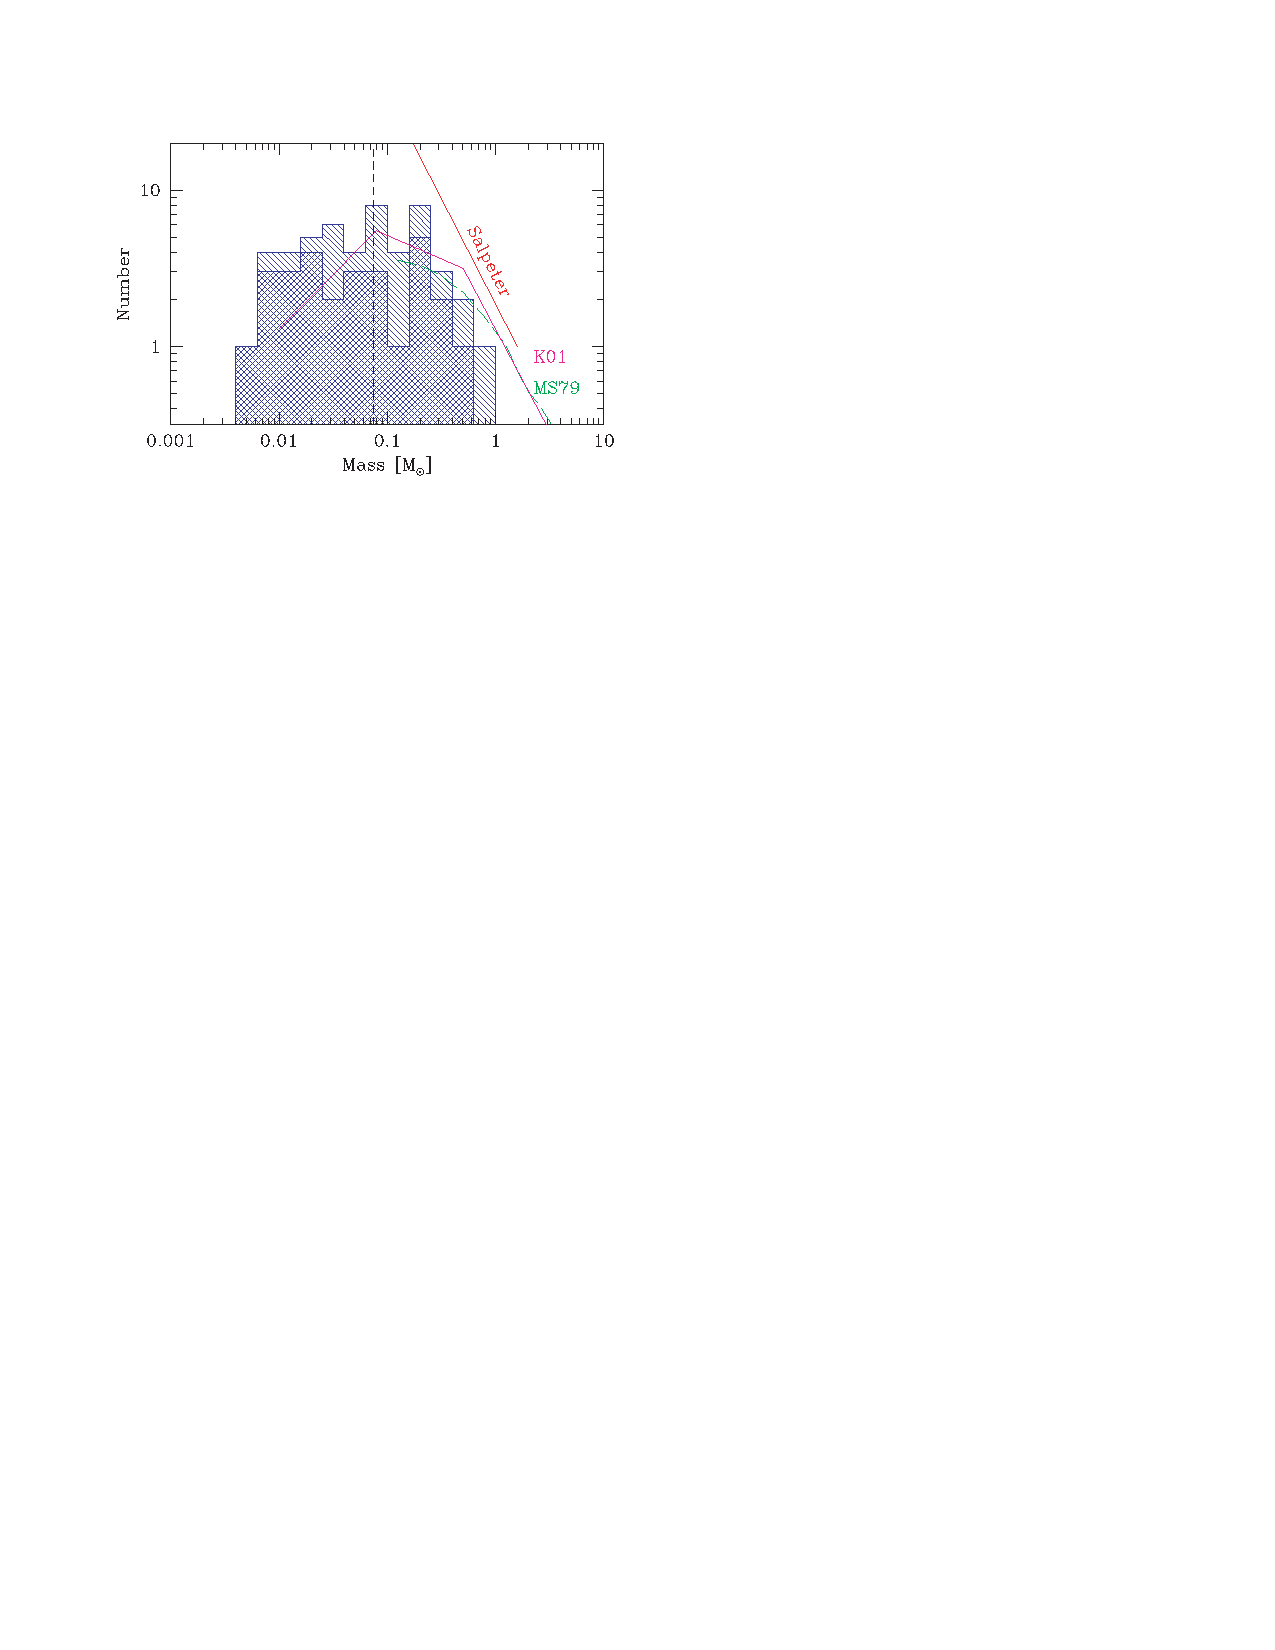
\includegraphics[width=0.8\textwidth]{background/Figures/F10_Bate2003.pdf}
\caption{Mass distribution resulting from the numerical simulation of \citet{2003MNRAS.339..577B}. The lines show the mass distributions of \citet{Salpeter1955}, \citet{1979ApJS...41..513M} and \citet{2001MNRAS.322..231K}. Reproduced from Figure 10 of \citet{2003MNRAS.339..577B}}
\label{fig:IMFBate2003}
\end{center}
\end{figure}

\begin{figure}[htbp]
\begin{center}
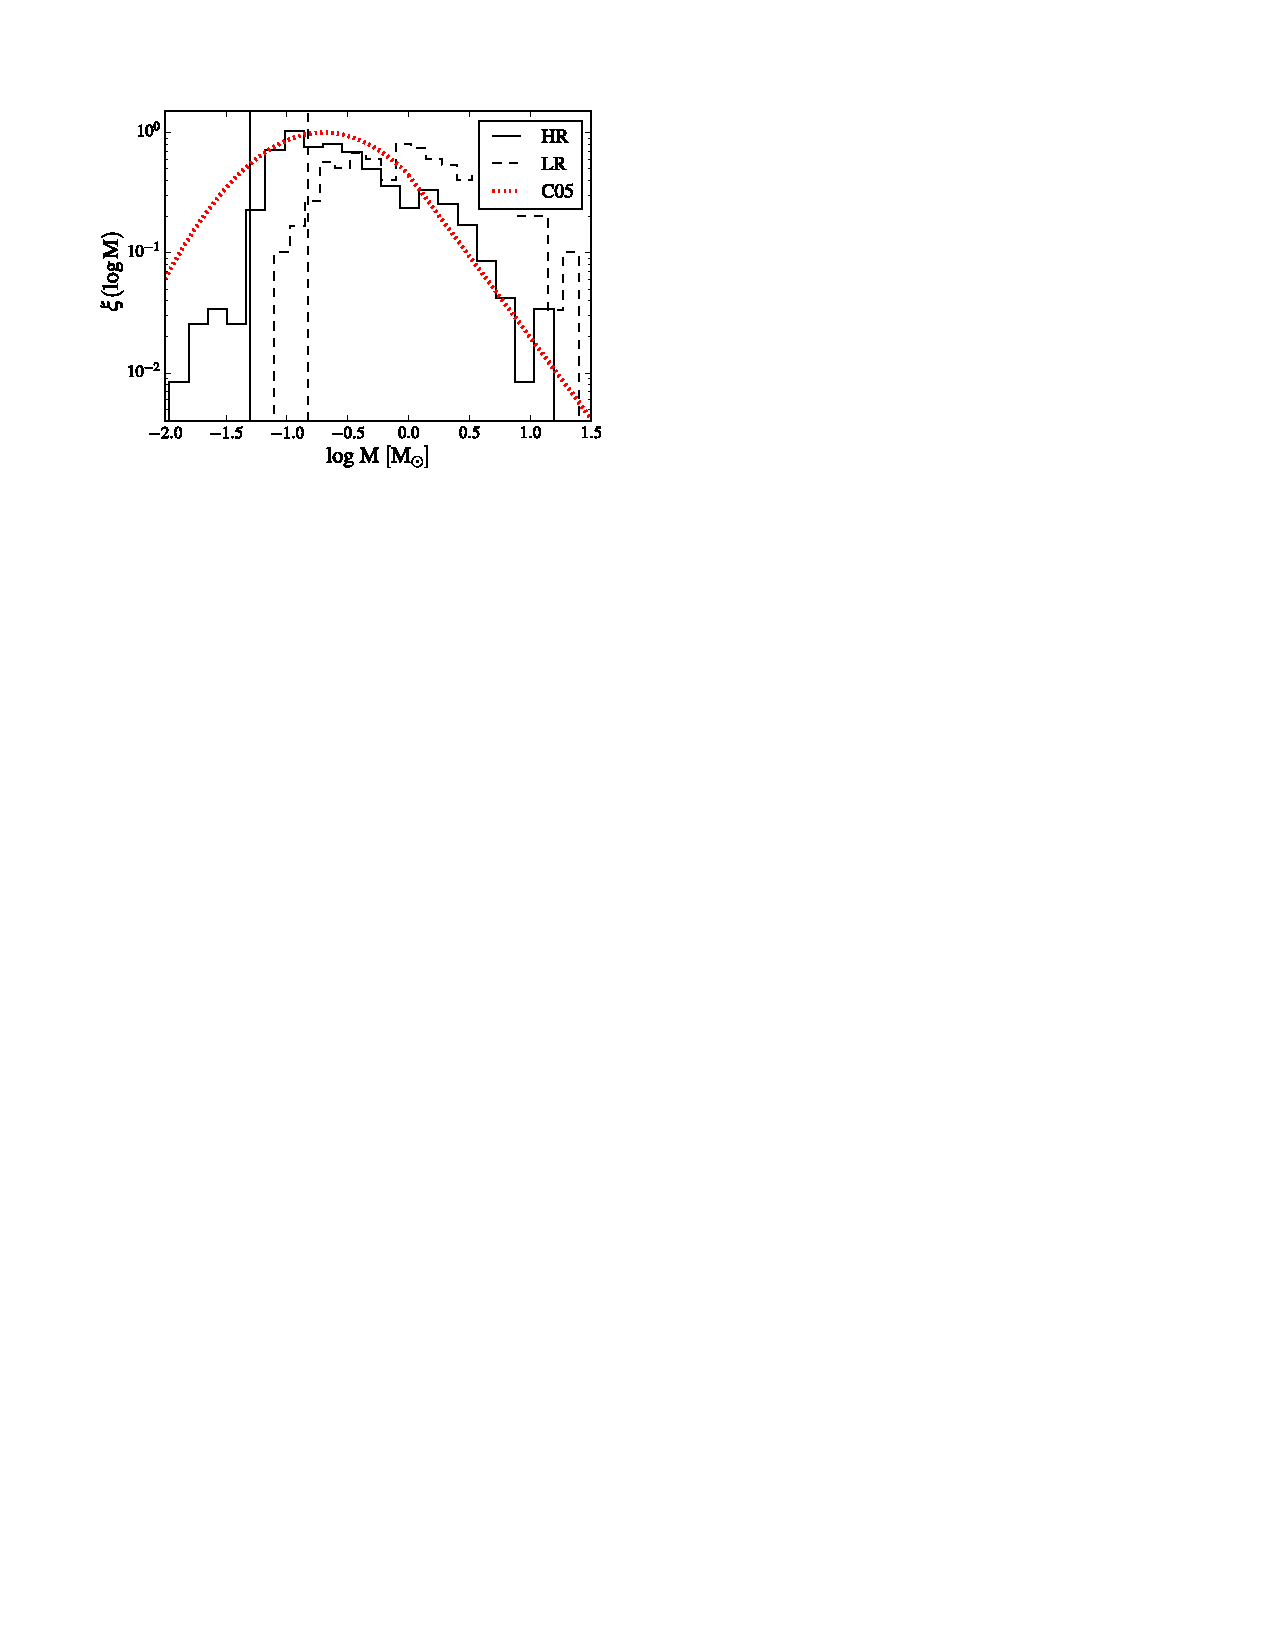
\includegraphics[width=0.8\textwidth]{background/Figures/F11_Kuznetsova2015.pdf}
\caption{Mass distribution resulting from the numerical simulation of \citet{2015ApJ...815...27K}. The High (solid line) and Low (dashed line) resolution simulations reach $0.05\, M_{\odot}$ and $0.15\, M_{\odot}$, respectively. Also shown the mass function of \citet{Chabrier2005} (red dashed line). Reproduced from Figure 11 of \citet{2015ApJ...815...27K}}
\label{fig:IMFKuznetsova}
\end{center}
\end{figure}

\section{The DANCe project}
\label{sect:DANCeproject}
It must be clear which is the objective

Description of the Nearby open clusters and their properties.

- List of open clusters in the DANce project.

- the importance of the pleiades, why we restrict to it.

It must be clear what are the limitations, the boundaries in which the objective will be searched

\section{Current methodologies}
\label{sect:current_methodologies}
Description of the current methodologies used to address the question mentioned previously.

- The works of Sarro, Krone-Martins, Malo, Gagne etc. LAcweing

-The advantages and caveats of the previous methodologies. 

-It must be clear the necessity of a new perspective

\section{The new tool}
\label{sect:newtool}

The proposal we made. The use of Bayesian Hierarchical Models. Benefits and issues of BHM.

Description of the advantages of BHM.

-> It must be clear that BHM are the best choice.

Description of the practical issues needed to be solved in order to use BHM.

MCMC techniques and  PSO.

-> It must be clear that MCMC methods are the best option.

Brief descriptions of our results and how they impact our current knowledge.

-> It must be clear that we attained the objective: The pleiades velocity, spatial and mass distributions.
 




%!TEX root = ../thesis.tex
\chapter{The Pleiades as a benchmark}
\label{chap:pleiades}

\section{Generalities}
\label{sect:generalities}
The ancient greeks named Pleiades to a crowded group of nine stars which they believed shared a common origin. These stars were the seven sisters, that together with their parents the titan Atlas and the nymph Pleione, were put in the sky  by the god Zeus.
 
Today, we call the Pleiades cluster not just to the nine stars that made up the original Pleione family, but to a much larger group, which according to \citet{Bouy2015} adds up to $\sim2100$ members. This cluster is fairly close to the sun, $\sim 134$ pc \cite[with parallaxes of $7.44\pm0.08$ and $7.48\pm0.03$ according to][respectively]{Galli2017,2017A&A...601A..19G}, and is also young in galactic scales, with only $\sim125$ \gls{myr} \citep{Stauffer1998}. Since it is located in the solar neighbourhood, it has a distinctive angular velocity in the plane of the sky: about $-16\,\mathrm{mas\cdot yr^{-1}}$ in right ascension and $20\,\mathrm{mas\cdot yr^{-1}}$ in declination. It has a metallicity near to the solar one \cite[{[Fe/H]$\sim$0},][]{Takeda2017}. Also, it has an almost null extinction of $A_v=0.12$ mag \citep{Guthrie1987}. These properties make the Pleiades one of the most studied clusters in the history of astronomy \footnote{Probably just after the Orion complex.}. Thus making it also the perfect test case of the methodology developed in this work.

As stated in the previous Chapter,  the objective of the present study is to obtain the statistical distributions of the distance, position, velocity, luminosity and mass of the Pleiades cluster. Thus, in the following sections I will describe the current knowledge of the Pleiades, concerning these astrophysical quantities. 
 
\section{The distance to the Pleiades}

\subsection{Measuring distances}
In astronomy, measuring distances is a complicated task. Techniques vary according to the distance scale that they aim to measure. The distance ladder is constructed from smaller to larger distances. The first step in this ladder is the distance to the sun. After that, the distance to the planets and then to the stars. This works deals only with nearby clusters, thus I only focus on measuring distances to these objects. 

The most direct way to measure distance to nearby stars is by means of the trigonometric parallax. This is the maximum relative angular displacement, with respect to the far distant stars, that an object suffers in the course of a year. {It is usually reported in miliarc seconds (mas)}. The relative displacement results from the movement of the Earth (thus of the observer) on its orbit around the sun. The relative displacement is maximal when measurements are taken at opposed points in the earth's orbit, when they are separated by six months. If the parallax were measured in seconds of arc and with infinite precision, then the distance to the object would be obtained by simply inverting its parallax. By doing so, the distance will be measured in parsecs. This unit gets its name from parallax-second. Thus an object located at a distance of one parsec from the sun shows a parallax of one arc second. The further the object is, the smaller the parallax gets.

As any measurement, parallaxes have uncertainties, which usually represent, or are a proxy for, the width of the distribution. {The parallax distribution is also continuous and non-limited}. 

When transforming parallaxes into distances we may be tempted to take a summary of the distribution, the mean for example, and just invert it to obtain the distance. This only holds if the summary corresponds to the true value (i.e. the statistic is unbiased). {The true value is that which would be observed in the presence of negligible uncertainties}. However, because measurements have uncertainties, which almost always are not negligible, the inversion of the parallax not always renders an unbiased estimate of the distance. {Assuming that the distribution of parallax measurements of an object is Gaussian, \citet{Lutz1973} found that the distance to the object can be reasonably recovered by just inverting the parallax if its relative uncertainty is below 0.15-0.20. However, the shape of the distribution of parallax measurements of an object (the second and higher order moments) plays also an important role. Transforming the parallax distribution into that of the distance require more than a simple inversion.}  

Several authors have proposed different approaches to the problem of distance determination using parallaxes, see for example \citet{Lutz1973,2015PASP..127..994B,2016ApJ...832..137A,2016ApJ...833..119A}. The proper way, as \citet{2015PASP..127..994B} points out, consists of inferring the true distances given the observed parallaxes. For that, a prior on the distance must be established. The authors mentioned before describe three different kinds of priors and the methodology needed to infer the true distances. However, going into deeper detail is beyond the scope of this work.

Now, I focus on the particular case of the distance to the Pleiades. One of the first measurements of the Pleiades distance using parallaxes was done by \citet{1999A&A...341L..71V} using \emph{Hipparcos} data.{ Later, the same author \citep{2009A&A...497..209V} refined his analysis and obtained a value of $120\pm1.9$ pc. However, \citet{2000ApJ...533..938G} with parallax measurements of seven stars taken at the Allegheny Observatory, and later \citet{2005AJ....129.1616S} with the parallaxes of three stars measured with the Fine Guidance Sensors of the \emph{Hubble Space Telescope}, derived distances of $130.9\pm7.4$ pc and $134.6\pm3.1$ pc, respectively. Finally, \citet{2014Sci...345.1029M} using very long baseline radio interferometric parallaxes of three stars obtained a distance of $136.2\pm1.2$ pc.} There was a clear controversy between \emph{Hipparcos} data and other parallax measurements. The current data release of the \gls{tgas}, gives a distance to the Pleiades of $133.7\pm0.5$ pc \cite[from a parallax of $7.48\pm0.03$ mas][]{2017A&A...601A..19G}. This seems to indicate that the \emph{Hipparcos} parallaxes were somehow biased.

Our research group finds a distance to the Pleiades of $134.4^{+2.9}_{-2.8} $ pc (from a parallax of $7.44\pm0.08$ mas) \citep{Galli2017}, which is in good agreement with the one of \gls{tgas}. We found this distance using the kinematic parallaxes delivered by the moving cluster technique. This essentially exploits the fact that since clusters are bound, their members show a clear kinematic footprint: they seem to converge to a point in the sky \citep{1964IAUS...20...50B}. Using this point and the velocity of the members (proper motion and radial velocities) it is possible to derive individual parallaxes. Furthermore, these individual parallaxes show a distribution which results from the dispersion of the cluster members distances along the line of sight. Figures \ref{fig:parallaxPhillip} and \ref{fig:parallaxTGAS} show the distribution of parallaxes for the Pleiades candidate members according to \citet{Galli2017} and \citet{2017A&A...601A..19G}, respectively. As can be seen from these Figures, the results of both works agree on the mean of the parallax distribution. However, they recover different variances. This difference results from the discrepancy in the number of objects, 1210 in \citet{Galli2017} vs. 152 in \citet{2017A&A...601A..19G}, and in the selection function of the two surveys. The \gls{tgas} sample is limited to the bright objects ($V \sim 11.5$ mag), whereas the \gls{ddr2} includes the faint end of the distribution ($i\sim25$ mag). For these reasons, in the following I adopt the distance found by \citet{Galli2017}.

Nevertheless, the distance distribution {(measured uncertainties comprised)} is only the depth component of the space distribution of the cluster, the other two components are given by the projected spatial distribution. 

\begin{figure}[ht!]
    \centering
    \begin{subfigure}[t]{\textwidth}
    \centering
        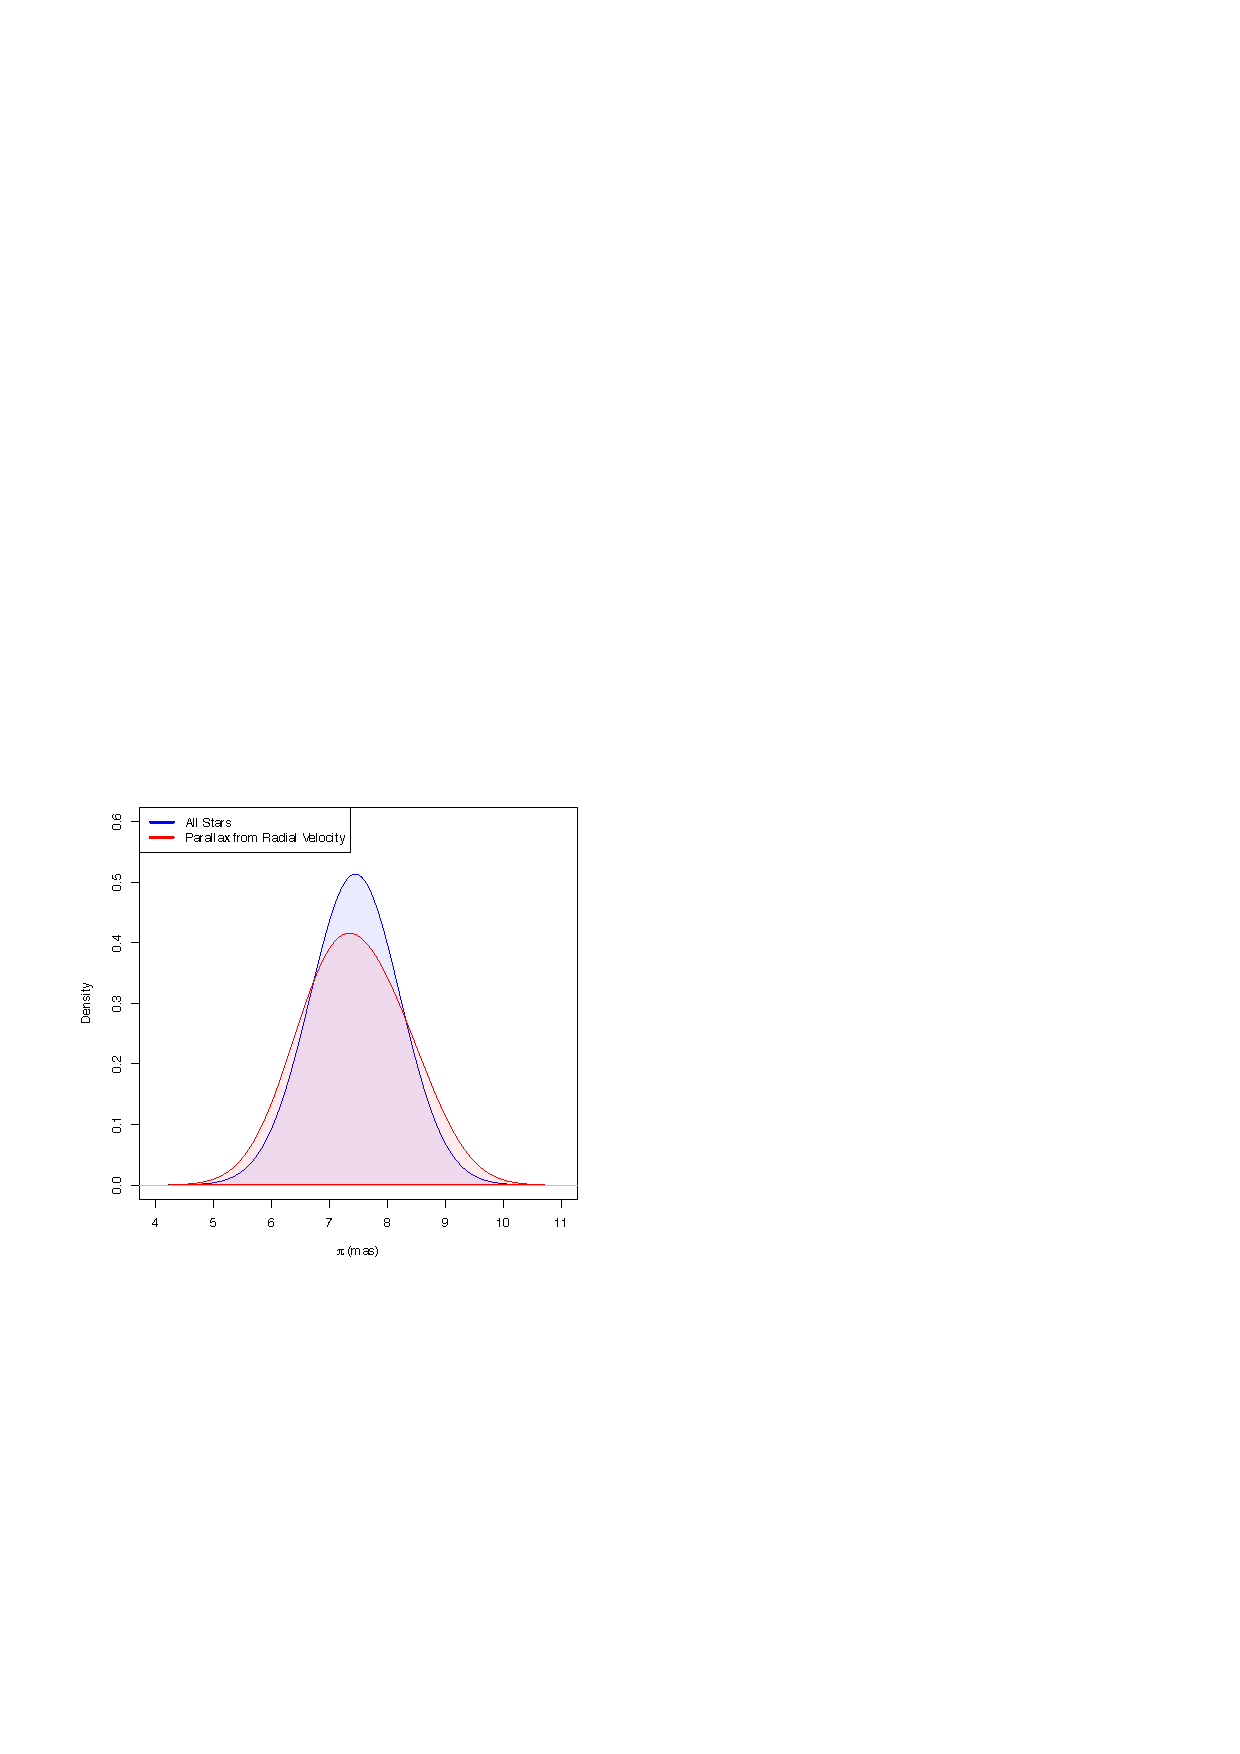
\includegraphics[height=8cm]{background/Figures/F13_Galli2017.pdf}
        \caption{Parallaxes according to \citet{Galli2017}. The red line shows all their candidate members (1210) while the blue one only those with known radial velocity (64). Reproduced from Figure 13 of \citet{Galli2017}, \textit{\usebibentry{Galli2017}{Title}}, \usebibentry{Galli2017}{Journal}, Vol. \usebibentry{Galli2017}{Volume}.}
        \label{fig:parallaxPhillip}
    \end{subfigure}
    \begin{subfigure}[t]{\textwidth}
    \centering
       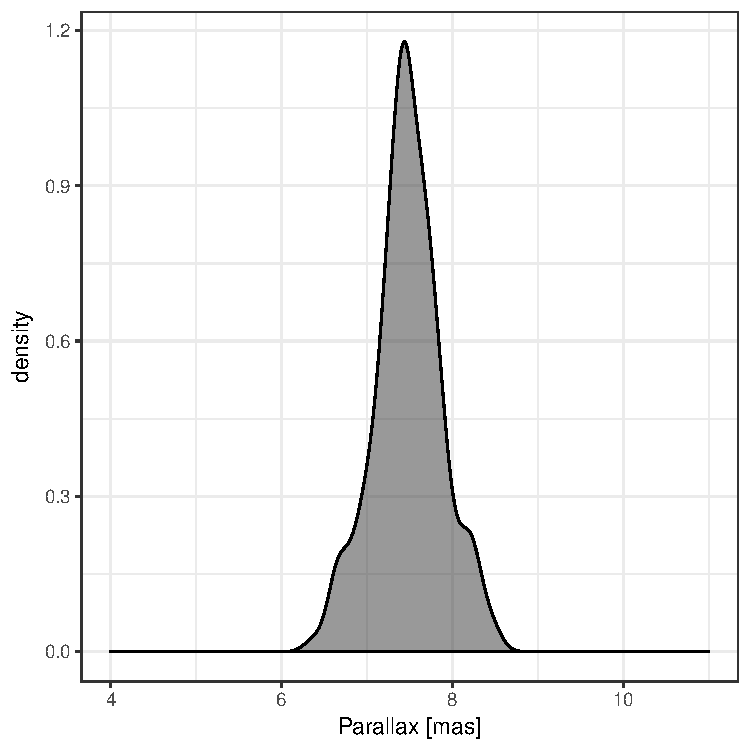
\includegraphics[height=8cm]{background/Figures/Parallax_GaiaCol2017.pdf}
        \caption{Parallaxes according to \citet{2017A&A...601A..19G}. Only their 152 candidate members.}
        \label{fig:parallaxTGAS} 
    \end{subfigure}
    \caption{Distribution of parallaxes for the Pleiades members.}
\end{figure}



\section{Projected spatial distribution}
\label{sect:PSD}
The \gls{psd} is the two dimensional projection, in the plane of the sky (the one perpendicular to the line of sight), of the cluster three dimensional space distribution. In astronomy, object positions are commonly measured in what is called the Equatorial Coordinate System\footnote{Another common coordinate system is the Alt-Azimuth one \cite[see][]{Smart1977}.}. It can be thought as the projection of the geographical coordinates, latitude and longitude, into the sky. The Right Ascension (R.A.) coordinate, analogous to the longitude, gives the objects angle with the vernal equinox, in an eastward direction and along the celestial equator. The Declination (Dec.) coordinate, analogous to the latitude, gives the object angle perpendicular to the celestial equator, positive to the North and negative to the South. For more details of the Equatorial Coordinate System see for example \citet{Smart1977}. 

{Stellar positions of an object are far more easily measured than its parallax. For this reason, just a small fraction of objects with stellar positions has also parallax measurements. In the case of the Pleiades, after cross-matching the \emph{Hipparcos} catalogue \citep{1997A&A...323L..49P} with the candidate members of \citet{Bouy2015}, I find that only 70 of the $\sim2100$ candidates have parallaxes. As seen in the previous section, this figure is roughly doubled with the new \gls{tgas} \citep{2016A&A...595A...1G} data release. In addition to the scarcity of parallaxes, which is expected to be solved with future \emph{Gaia} data releases, the relative uncertainties in R.A. and Dec. coordinates, measured in degrees, are far better ($\sim 10^{-5}$) than those of the parallaxes ($\sim10^{-1}$), measured in mas. Transforming these relative precisions into parsecs, by means of the distance, it is seen that the position in the plane of the sky is $10^4$ more precise than along the line of sight.  These two are the main reasons, for which the Pleiades space distribution has been studied mainly through its \gls{psd}. The latter has been the subject of several studies. }

One of the earliest results of the Pleiades \gls{psd} was done by \citet{Limber1962}. He used a mixture of four indices polytropic distribution, as was described is his earlier \citet{Limber1961} work, to fit the \gls{psd} of the 246 candidate members of \citet{Trumpler1921}. These candidates were contained in a $3^{\circ}$ radius around \emph{Alcyone} (one of the central most massive stars of the Pleiades cluster). 

\sloppy
Later, \citet{Pinfield1998} fitted King profiles \citep{King1962} to candidate members from the literature, which were contained in a $3^{\circ}$ radius area. They fitted King profiles to objects within different mass ranges, their bins centred at $5.2,1.65,0.83$ and $0.3 \,\mathrm{M_{\odot}}$. The tidal radius they found, $13.1\,pc$ ($\sim 5.6^{\circ}$) contained $1194$ candidate members. The total mass of these members amounted to $735\,\mathrm{M_{\odot}}$. These authors also estimated a mean individual stellar mass of $0.616\,\mathrm{M_{\odot}}$. {They measured core radius in the 0.9 to 2.91 pc range for the King profiles fitted to their different mass bins.}

On the same year \citet{Raboud1998} also fitted a King's profile \citep{King1962} to a list of 270 candidate members with masses in the range $0.74-7.04\,\mathrm{M_{\odot}}$, which were contained within a $5^{\circ}$ radius area. They found a core radius of $1.5$ pc and a tidal radius of $17.5$ pc ($7.5$ degrees). Using different approaches, they derived a total mass within the range of $500 -8000 \,\mathrm{M_{\odot}}$. They also measured an ellipticity of $\epsilon=0.17$, however they did not make any explicit mention on the position angle of the axis of the ellipse.

Later, \citet{Adams2001} also fitted a King profile to objects with membership probabilities $p>0.3$ within a radius of $10^{\circ}$. They found a core radius of $2.35-3.0$ pc and a tidal radius of $13.6-16$ pc ($5.8 - 6.8^{\circ}$). They estimate a total mass of $\sim 800\,\mathrm{M_{\odot}}$, and their measured ellipticities are in the range $0.1-0.35$. 

\citet{Converse2008} fit a King profile to a sample of 1245 candidate members from \citet{Stauffer2007} compilation. These objects have masses greater than $0.08\,\mathrm{M_{\odot}}$ and are contained within a $5^{\circ}$ radius. They obtained a tidal radius of $18$ pc (7.7 degrees) and a core radius of  $1.3$ pc. Later, \citet{Converse2010} refined their study and obtained a core radius of $2.0\pm0.1$ pc, a tidal radius of $19.5 \pm 1.0 $ pc ($\sim 8.3$ degrees) and a total mass of $870\pm35\,\mathrm{M_{\odot}}$. In Fig. \ref{fig:spatialConverse}, I reproduce the surface density fit obtained by these authors.

The previous summary of results shows at least two interesting points. In the first place, King profile \citep{King1962} has been the preferred choice for the Pleiades cluster, although it was created to fit the \gls{psd} of globular clusters. Since globular clusters are farther away than open clusters and in a low density environment, usually the end of their \gls{psd} is well within the survey area. The second point concerns the increasing trend of the tidal radius with the size of the survey and the publication date, see Table \ref{tab:tidal_iterature}. As the surveys increase in area the derived tidal radii increase as well. The exception is the work of \citet{Adams2001}. Since these authors used low membership probability ($\geq0.3$) objects, they may have also fitted the field. The surface density of a tidally truncated cluster should diminish with radius and eventually go to zero at the tidal radius. However, as can be seen in Figure \ref{fig:spatialAdams}, where I reproduce Figure 8 of \citet{Adams2001}, their surface density remains almost constant after $5^{\circ}$. This may be an indication of contamination in their sample. Furthermore, as those authors mention, they expect that the contamination dominates their sample outside the $5^{\circ}$ radius.

The two points mentioned before are tightly related. With the exception of the work of \citet{Adams2001}, the coverages of the rest of the surveys have not reached their estimated tidal radius. It indicates that the sample of members we currently have is spatially biased. It only contains objects from the inner parts of the cluster. Thus, estimates of the tidal radius may also biased. Nevertheless, this issue will be addressed with the full sky coverage of \emph{Gaia's} data.

\begin{figure}[ht!]
    \centering
    \begin{subfigure}[t]{0.49\textwidth} \centering
        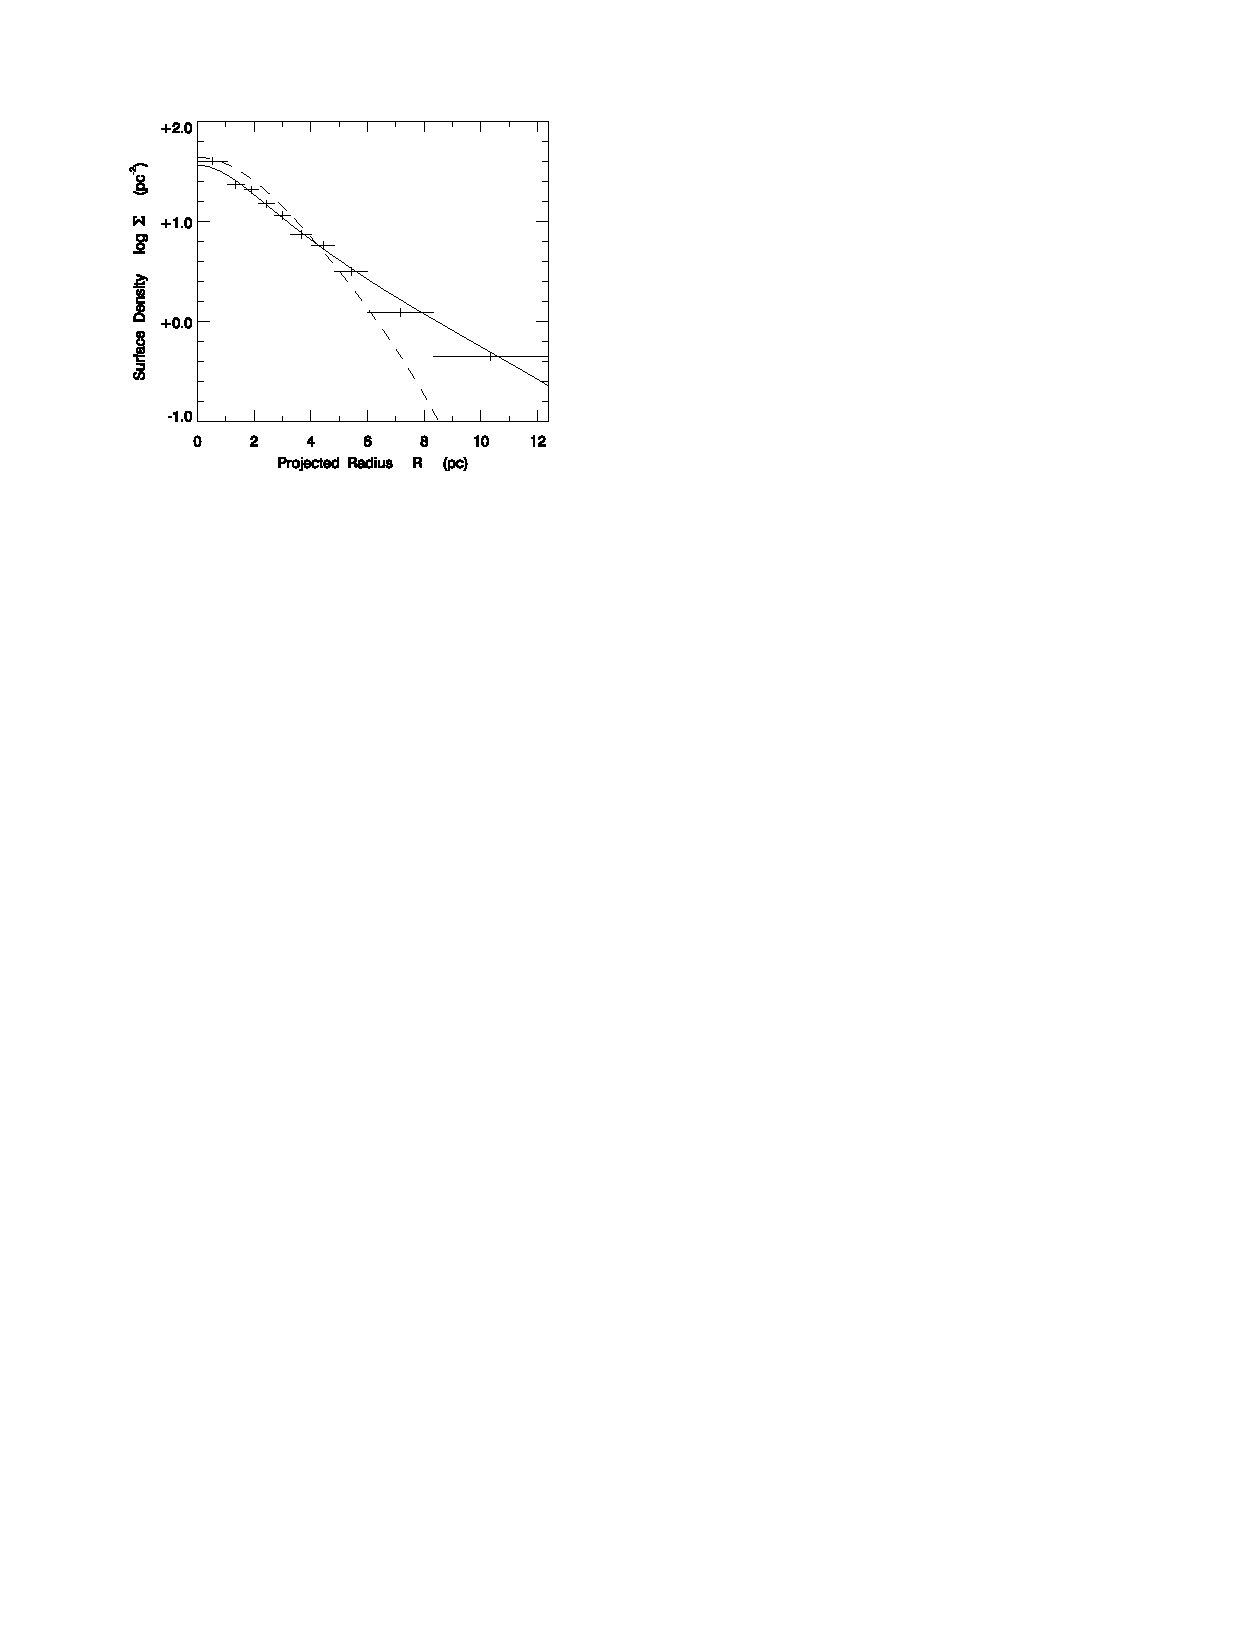
\includegraphics[height=6cm]{background/Figures/F1_Converse2010.pdf}
        \caption{}
        \label{fig:spatialConverse}
    \end{subfigure}
    \begin{subfigure}[t]{0.49\textwidth} \centering
       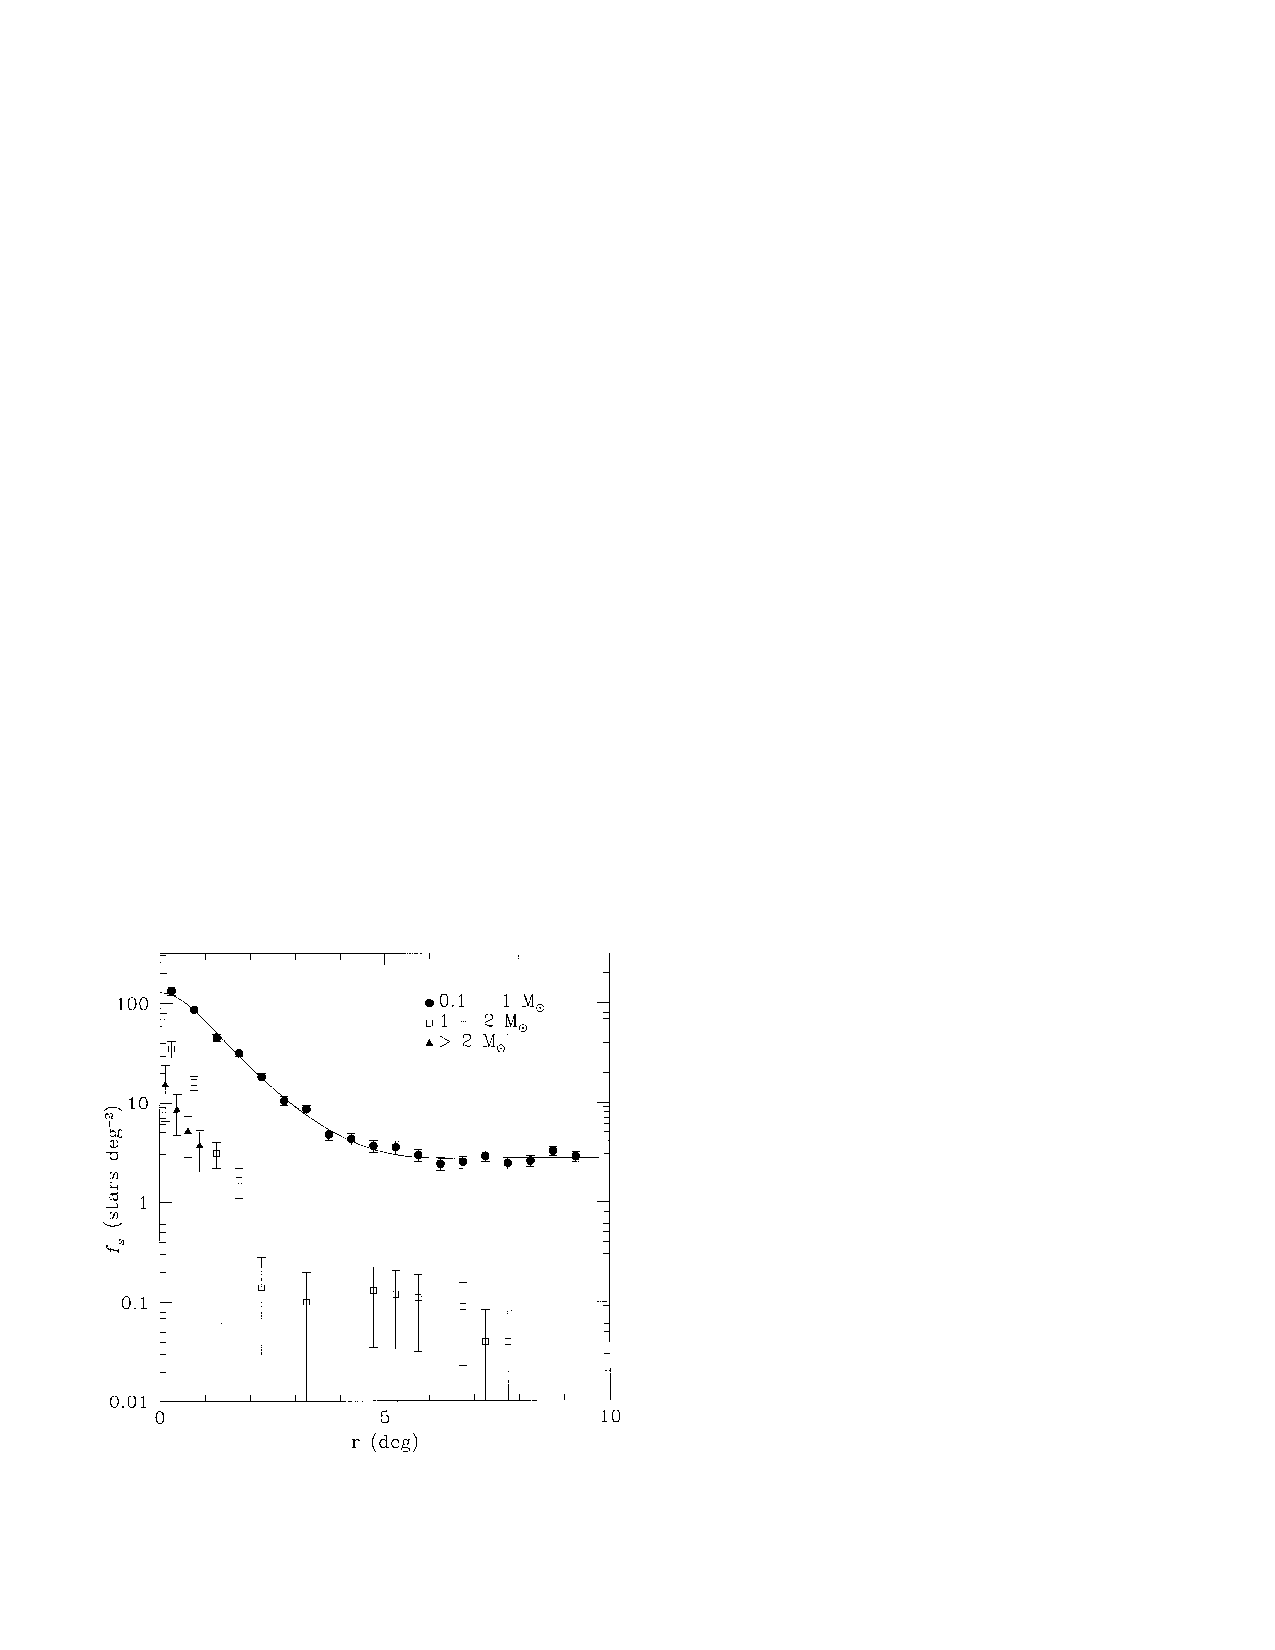
\includegraphics[height=6cm]{background/Figures/F8_Adams2001.pdf}
        \caption{}
        \label{fig:spatialAdams} 
    \end{subfigure}
    \caption{Projected spatial distribution of the Pleiades cluster. (a) Results from  \citet{Converse2010}. The crosses, and the dashed and solid lines represent the data and the fitted polytrope and King profile, respectively. Reproduced from Figure 1 of \citet{Converse2010}, \textit{\usebibentry{Converse2010}{Title}}, \usebibentry{Converse2010}{Journal}, Vol. \usebibentry{Converse2010}{Volume}. (b) Results from \citet{Adams2001}. The line shows the fitted King profile while the symbols are for different mass bins used. Reproduced from Figure 8 of \citet{Adams2001}, \textit{\usebibentry{Adams2001}{Title}}, \usebibentry{Adams2001}{Journal}, Vol. \usebibentry{Adams2001}{Volume}.}
\end{figure}

\begin{table}[ht!]
\caption{Survey, and derived core and tidal radius for recent studies in the literature. }
\begin{center}
\begin{tabular}{ccccc}
Authors &Core&Tidal& Tidal & Survey\\
&radius&radius&radius&radius\\
&(pc)&(pc)&($^\circ$)&($^\circ$)\\
\hline
\citet{Pinfield1998}&0.9-2.91&13.1&5.6&3\\
\citet{Raboud1998}&1.5&17.5&7.5&5\\
\citet{Adams2001}&2.35-3.0&16&6.8&10\\
\citet{Converse2008}&1.3&18&7.7&5\\
\citet{Converse2010}&2.0&19.5&8.3&5\\
\hline
\end{tabular}
\end{center}
\label{tab:tidal_iterature}
\end{table}%

  
\section{Velocity Distribution}

The three dimensional velocity distribution of the Pleiades has also been studied using its projections. One of them goes along the line of sight, it corresponds to the radial velocity. The other one is perpendicular to the previous one, lies in the plane of the sky, and corresponds to the transverse velocity. It is derived from  proper motions. These are angular velocities obtained after measuring the angular displacement of the object in at least two different epochs. Again, measuring the individual stellar position and its displacement over time is far easier than measuring radial velocities. These are measured using the Doppler shifted absorption lines in the spectre of the object. This shift is proportional to the object velocity relative to the observer along the line of sight. 

Since radial velocities require the object spectrum, their obtention for all cluster members, and particularly for the fainter ones, will demand a large amount of observing time. On the other hand, wide field images have been available for quite a long time, thus allowing long time base lines to measure proper motions.  Nevertheless, due to the Pleiades distance, radial velocities are often more precise than proper motion measurements, usually on the $1 \,\mathrm{km\cdot s^{-1}}$ regime. For these reasons, historically, the velocity distribution of the Pleiades cluster has been studied through the proper motions of its members. 

Probably the first description of the \gls{tvd} of the Pleiades is that of \citet{1884MNRAS..44..355P}. Using archival data from  Königsberg (1838-1841), Paris(1874) and Oxford (1878-1880) observatories, together with his own \emph{Differential Micrometer} observations, he was able to observe the relative displacements of 40 Pleiades stars. According to him \citep{1884MNRAS..44..355P}: \textit{the relative displacements of these distant suns, although not distinctly and accurately measurable in numerical extent, appear to vary both in direction and amount; indicating thereby the mutual influence of a group of gravitating bodies.} 

Later, \citet{Trumpler1921} used, for the first time, proper motion measurements to identify the members of the Pleiades cluster. He classified objects as candidate members according to the distance they show, in the proper motion space, to the mean proper motion of the cluster. This mean was previously calculated by Boss in his \emph{Preliminary General Catalog} \citep{1910pgcs.book.....B}. So far as my historic research went, Boss' work was the first measurement of a statistic of the \gls{tvd} of the Pleiades. 

Later \citet{1938AJ.....47...25T}, using Trumpler's data and archival compilations, was able to measure the dispersion of the proper motions distribution. He estimated it to be $0.79\,\mathrm{mas\cdot yr^{-1}}$($0.65\,\mathrm{ km\cdot s^{-1}}$ at 136 pc). This was probably, the first measurement of the second moment of the spatial velocity distribution. From this value he then derived a total mass of $260\,\mathrm{M_{\odot}}$.

In recent years \citet{Pinfield1998} used the velocity dispersion to probe that the cluster was in an state near to the virial equilibrium. Later, \citet{2006ARep...50..714L} used the projected radial and tangential velocity components of the spatial velocity distribution of 340 members to claim the absence of evidence for rotation, expansion or compression of the cluster. Also, he also found no evidence to support mass segregation. 

Concerning the radial velocities, the first record for the Pleiades correspond to \citet{1904ApJ....19..338A}. He measured the radial velocities of the six brightest stars. After this seminal work, more than a dozen of works have been published. Among them are the works of \citet{1924PhDT.........1W,1944ApJ...100..360S,1979BICDS..16....2M,1991ApJ...377..141L,1992A&A...255..130R,1994AJ....108..160S,1997A&A...320...74M,1996ApJ...469..706M,2000AJ....119.1303T,2006ARep...50..714L,2009AAS...21340702W,2009A&A...498..949M}, and \citet{2013AJ....146..134K}. In previous studies, the typical number of Pleiades candidate members was below 100 objects, with the works of \citet{2009AAS...21340702W} and \citet{2009A&A...498..949M} reaching 269 and 275 objects, respectively. The latest compilation of radial velocities from the literature is the one made made by \citet{Galli2017}. This list contains measurements for 394 objects. The distribution of these radial velocities is almost gaussian with a centre at $5.6\,\mathrm{km \cdot s^{-1}}$. In \citet{Galli2017}, we estimated a velocity dispersion of the $0.8\,\mathrm{ km\cdot s^{-1}}$ for the Pleiades candidate members.

Although, transverse and radial velocities are useful projections, the dynamical analysis of the cluster demands the three dimensional distribution. In \citet{Galli2017} we provide a list of 64 cluster members with full spatial velocities. The distributions of the three projections of these spatial velocities are shown in Figure \ref{fig:velocityGalli}.

\begin{figure}[ht!]
\begin{center}
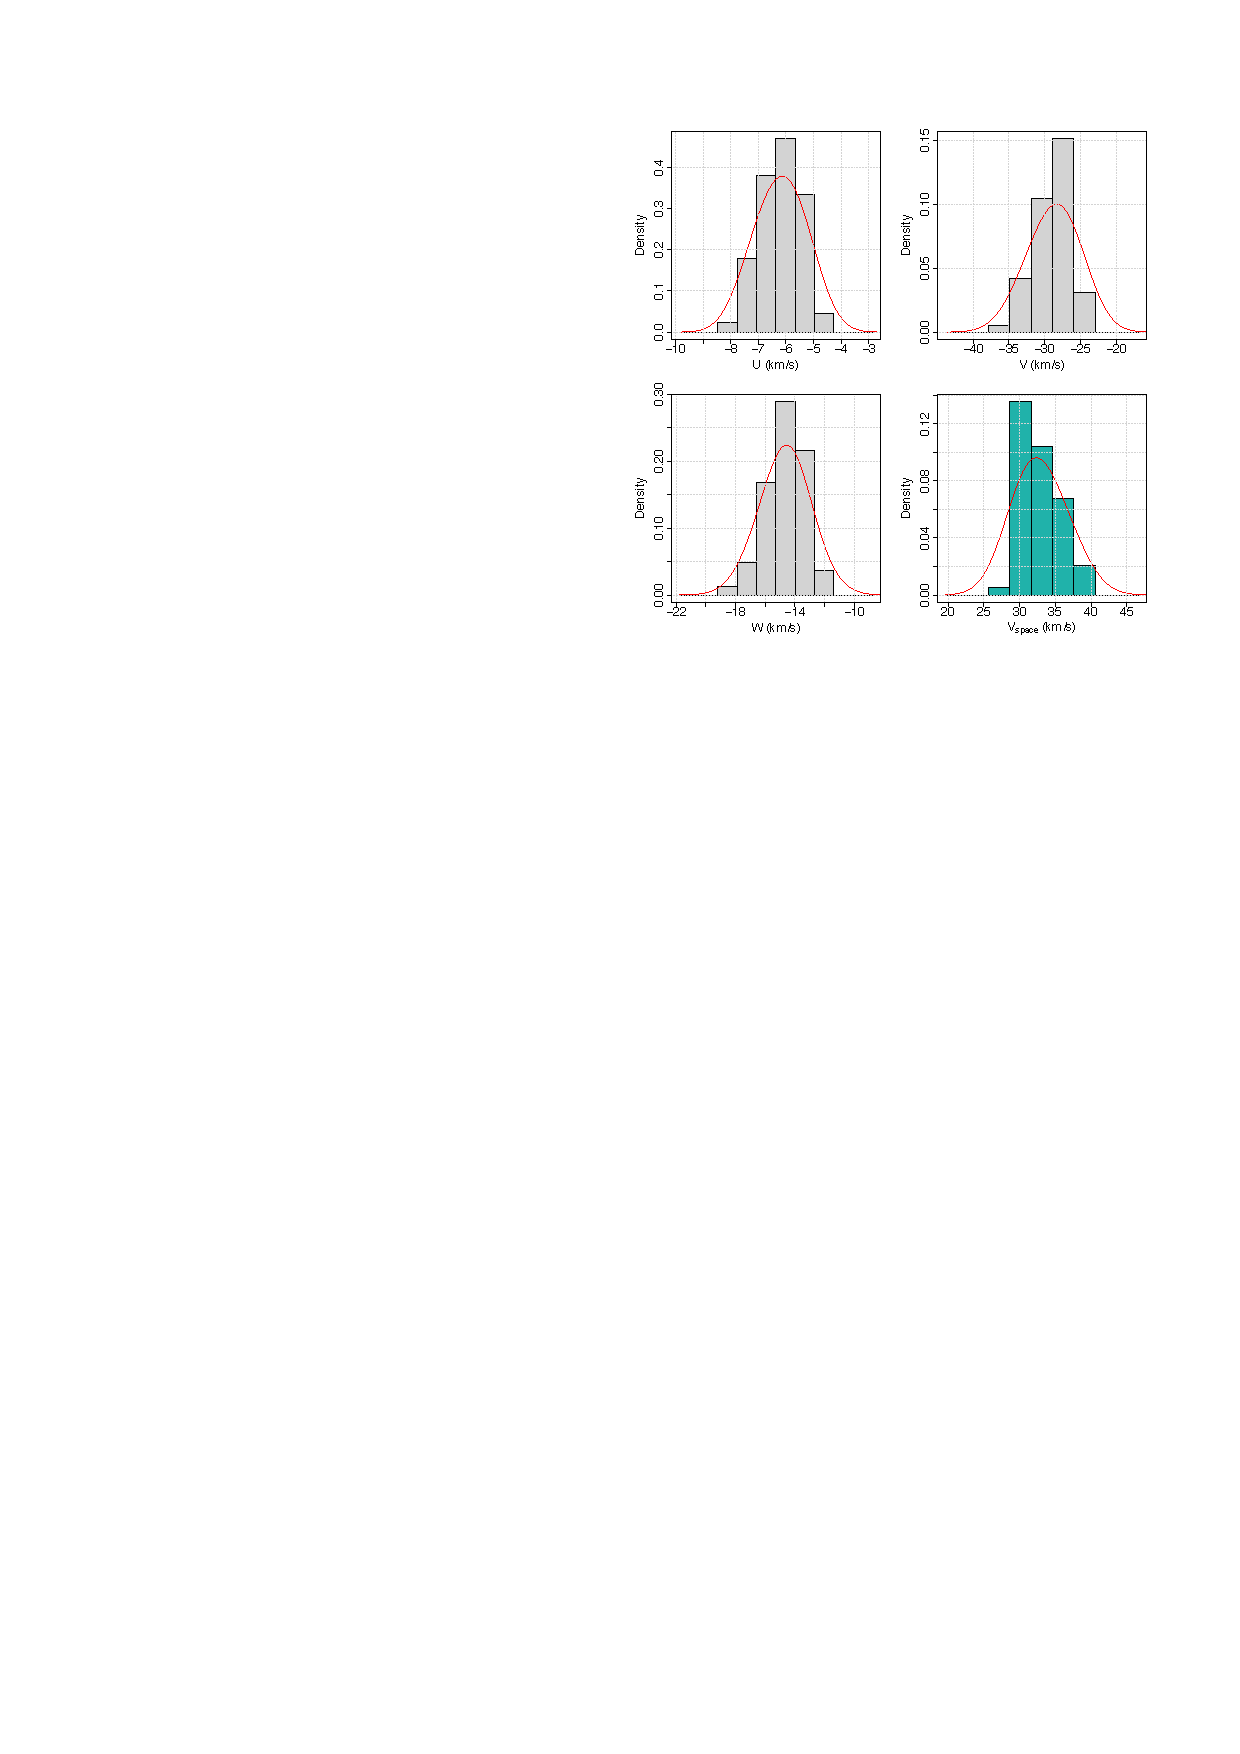
\includegraphics[width=0.8\textwidth]{background/Figures/F11_Galli2017.pdf}
\caption{Histogram and kernel density estimation (red line) of the components (grey) and modulus (green) of the spatial velocity distribution of 64 candidate members of \citet{Galli2017} with radial velocities and parallaxes. Reproduced from Figure 11 of \citet{Galli2017}, \textit{\usebibentry{Galli2017}{Title}}, \usebibentry{Galli2017}{Journal}, Vol. \usebibentry{Galli2017}{Volume}.}
\label{fig:velocityGalli}
\end{center}
\end{figure}

\section{Luminosity Distribution}

The luminosity distribution usually refers to the statistical probability distribution of the absolute\footnote{The absolute magnitude $M$, is the brightness that an object of apparent magnitude $m$ will show at a distance of 10 pc.} magnitude of the cluster population. It can also refer to the distribution of apparent magnitudes. It can be thought as the spectrum of brightness of the cluster members. Its importance lies in the fact the the luminosity of a star, measured in absolute magnitudes, can be related to its mass by the mass-luminosity relation. Therefore, the luminosity distribution is a proxy for the mass distribution. 

The study of the distribution of luminosities in the Pleiades started few years later than those of the positions and proper motions. The first record I found on the luminosity distribution is the one of \citet{Trumpler1921} (see Fig. \ref{fig:luminosityTrumpler}). He computed the number of stars in each magnitude bin for his two samples of candidate members, those comprising the objects within the central $1^{\circ}$, and those between $1^{\circ}$ and $3^{\circ}$, referred as Tables I and II, respectively. The completeness of the inner and outer samples was estimated at 14.5 and  9.8 photographic magnitudes (roughly 14 and 9 in the visual band), respectively. He observed that the luminosity distributions of these two samples were not alike, with the inner sample being brighter than the outer one. He also noticed that the luminosity distribution is not smooth, and shows a local minimum at 9 magnitudes, then an abrupt rise. Both effects are present in the two samples.

\begin{figure}[ht!]
\begin{center}
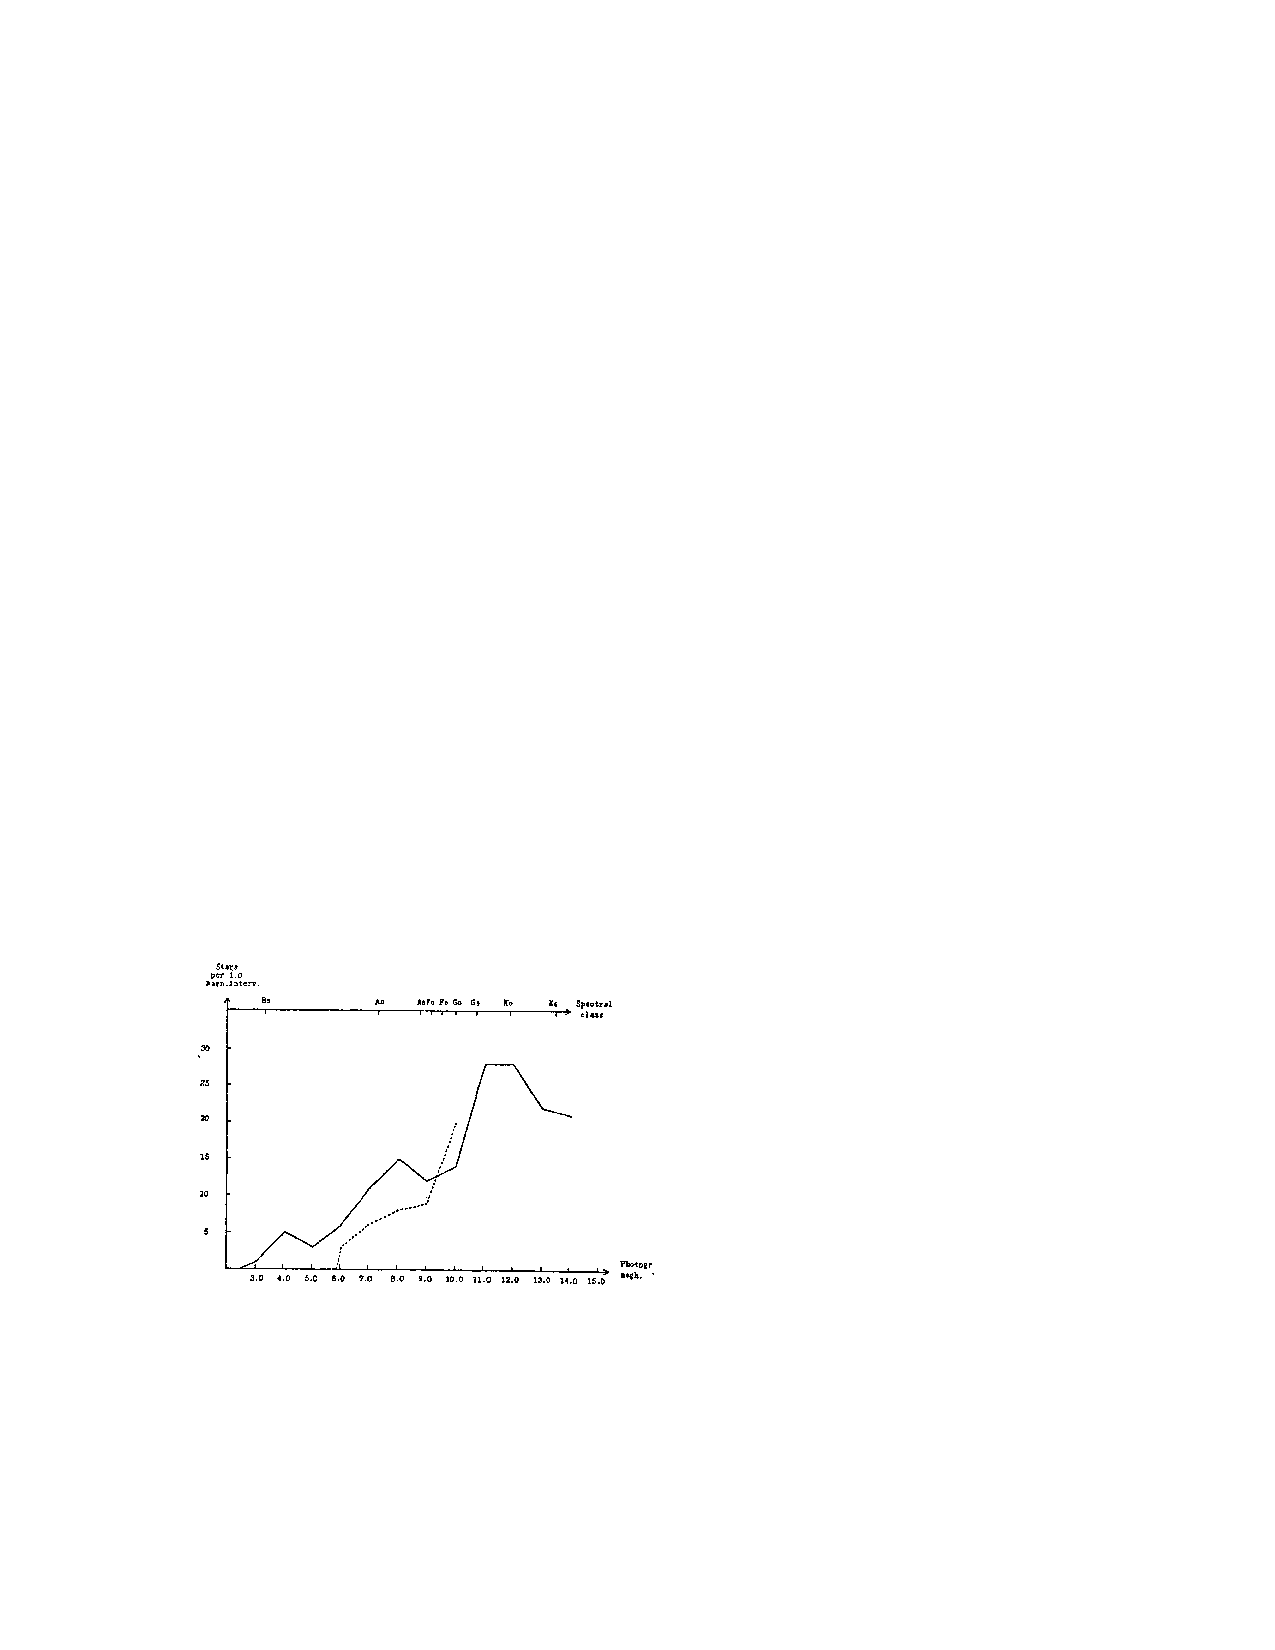
\includegraphics[width=\textwidth]{background/Figures/F2_Trumpler1921.pdf}
\caption{Luminosity distribution according to \citet{Trumpler1921}. The solid and dashed lines correspond to objects within $1^{\circ}$ and within $1^{\circ}$, and $3^{\circ}$ from the centre. Reproduced from Figure 2 of \citet{Trumpler1921}, \textit{\usebibentry{Trumpler1921}{Title}}, \usebibentry{Trumpler1921}{Journal}, Vol. \usebibentry{Trumpler1921}{Volume}.}
\label{fig:luminosityTrumpler}
\end{center}
\end{figure}

Later, \citet{Johnson1958} obtained the luminosity distribution using a sample of 289 candidate members. They assessed  membership solely on photometry. Their luminosity distribution is shown in Fig. \ref{fig:luminosityJohnson}

\begin{figure}[ht!]
\begin{center}
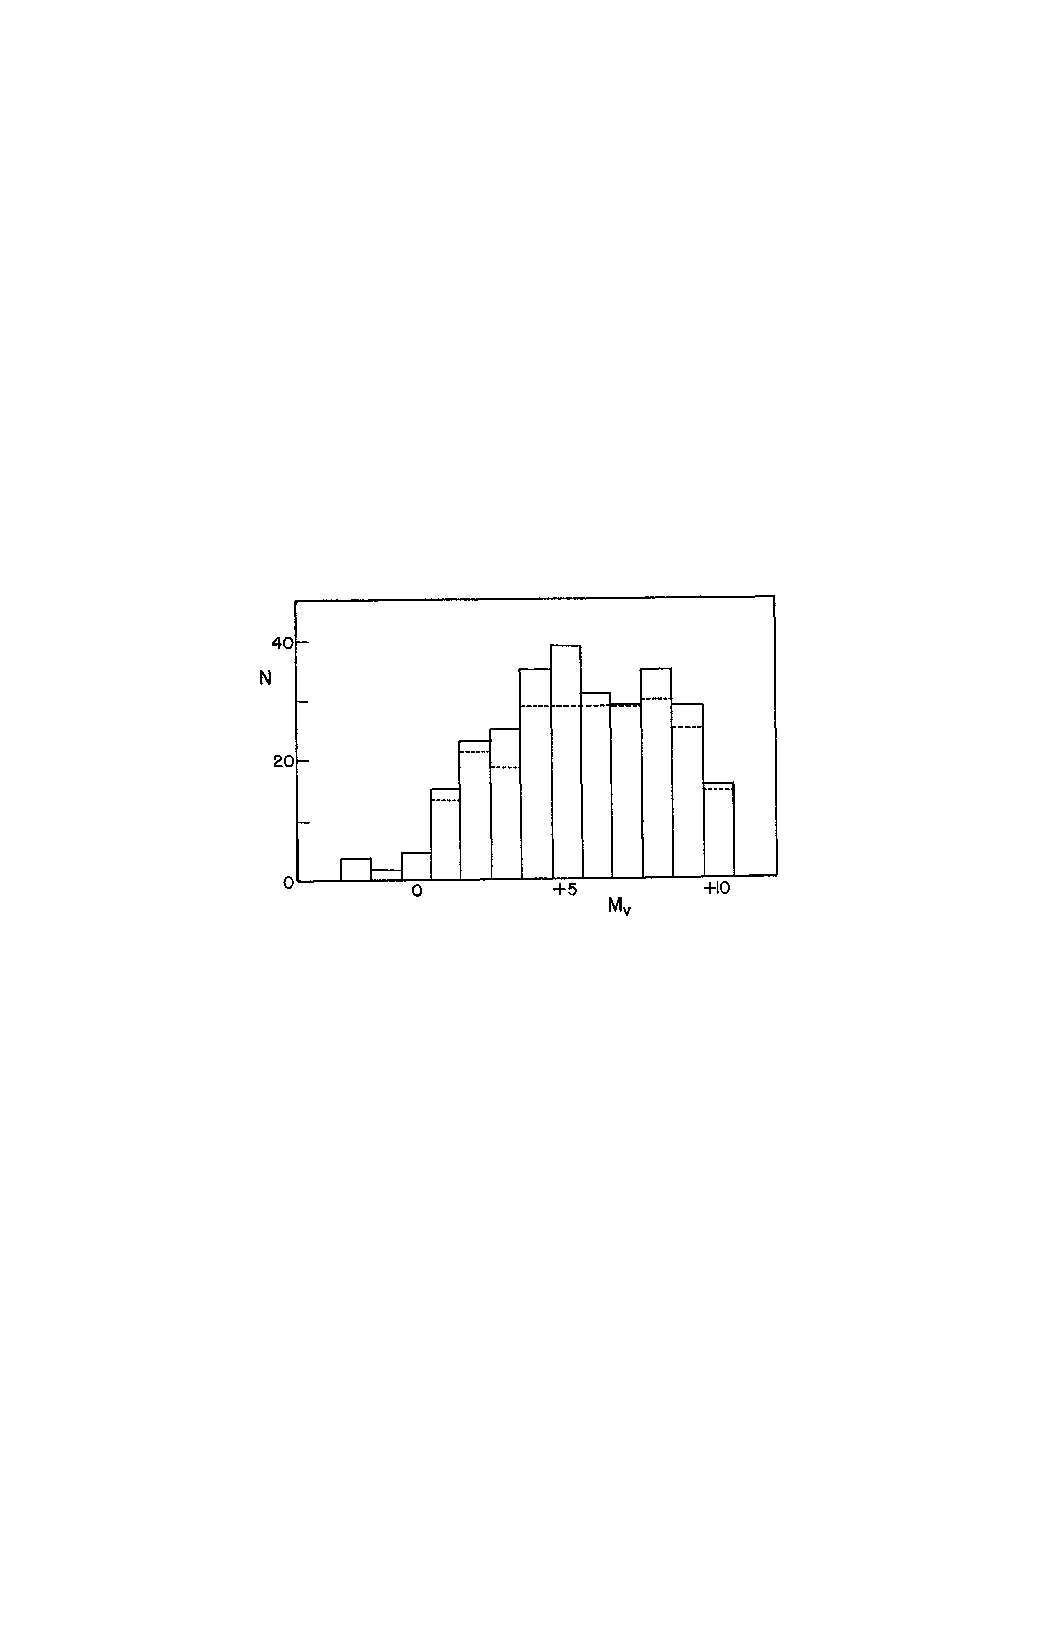
\includegraphics[height=8cm]{background/Figures/F3_Johnson1958.pdf}
\caption{Luminosity distribution in the visual band according to \citet{Johnson1958}. The dotted line represent the counts of main sequence stars only. Reproduced from Figure 3 of \citet{Johnson1958}, \textit{\usebibentry{Johnson1958}{Title}}, \usebibentry{Johnson1958}{Journal}, Vol. \usebibentry{Johnson1958}{Volume}.}
\label{fig:luminosityJohnson}
\end{center}
\end{figure}

Later, \citet{Limber1962} compared the luminosity distributions derived from the data of \citet{Trumpler1921}, \citet{Hertzsprung1947}, and \citet{Johnson1958}, with the initial luminosity distribution that he derived \citep{Limber1960}. The initial luminosity distribution corresponds to the distribution of luminosities that the cluster had at the moment of formation. \citet{Limber1960} derived it mixing data of galactic clusters and the local neighbourhood, and later correcting it by effects of age. He noted that the Pleiades present day luminosity distribution starts to differ from the initial luminosity distribution at visual magnitude $5.5$, see Fig. \ref{fig:luminosityLimber}. Assuming that this difference is due to the fact that stars fainter than $5.5$ have not yet had enough time for contraction, he derives an age of 50 \gls{myr}. 

\begin{figure}[ht!]
\begin{center}
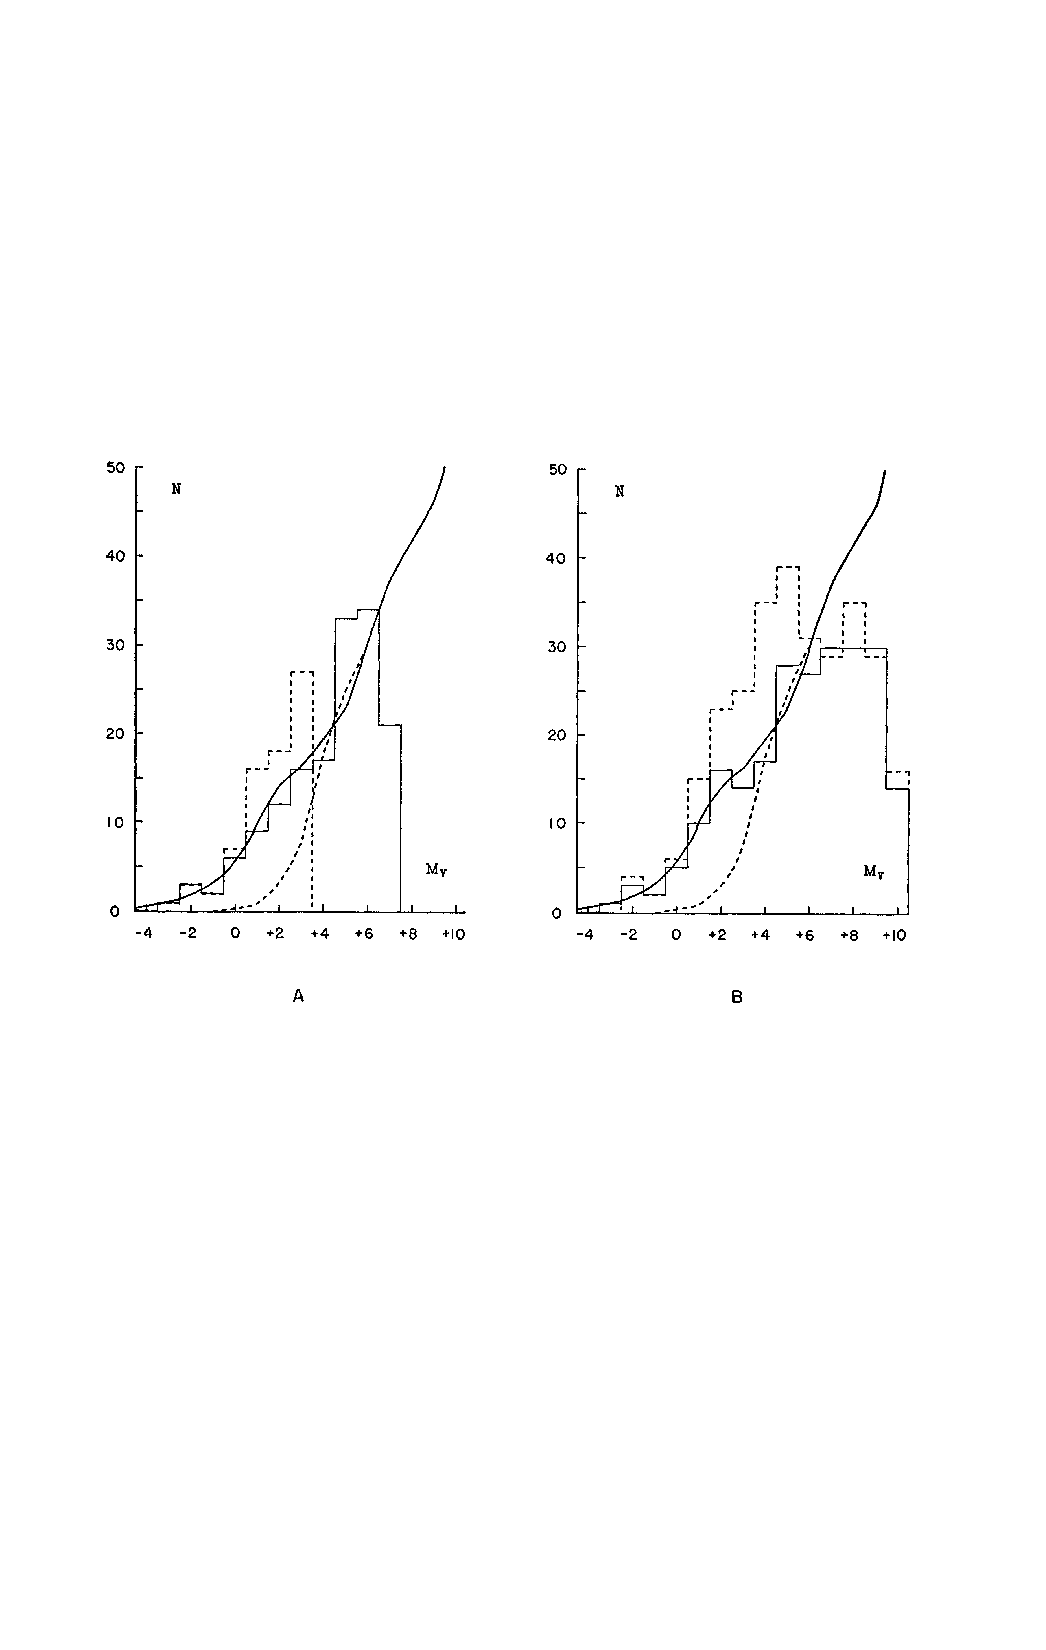
\includegraphics[height=8cm]{background/Figures/F4_Limber1962.pdf}
\caption{Luminosity distribution in the visual band according to \citet{Limber1962}.The solid and dashed histograms in: A correspond to \citet{Trumpler1921} data from the Tables II and I, respectively, in B, correspond to the data from \citet{Hertzsprung1947} and \citet{Johnson1958}, respectively. The solid and dashed curves line represent initial luminosity distribution and the present day luminosity distribution of the solar neighbourhood, respectively, both from \citet{Limber1960} . Reproduced from Figure 4 of \citet{Limber1962}, \textit{\usebibentry{Limber1962}{Title}}, \usebibentry{Limber1962}{Journal}, Vol. \usebibentry{Limber1962}{Volume}.}
\label{fig:luminosityLimber}
\end{center}
\end{figure}

In recent years, the luminosity distribution has been described in the works of \citet{Lodieu2012} and \citet{Bouy2015}. 
\citet{Lodieu2012}, using the \emph{UKIDSS} DR9 survey for galactic clusters and a probabilistic membership selection method (see discussion in Chapter \ref{chap:introduction}) based on proper motions only, and proper motions and photometry, found 8797 and 1147 candidate members, respectively. However, they do not provide the contamination rate in their analysis. Using both lists, they provide their luminosity distributions in the $Z$ band, which I show in Fig. \ref{fig:luminosityLodieu}.

\begin{figure}[ht!]
\begin{center}
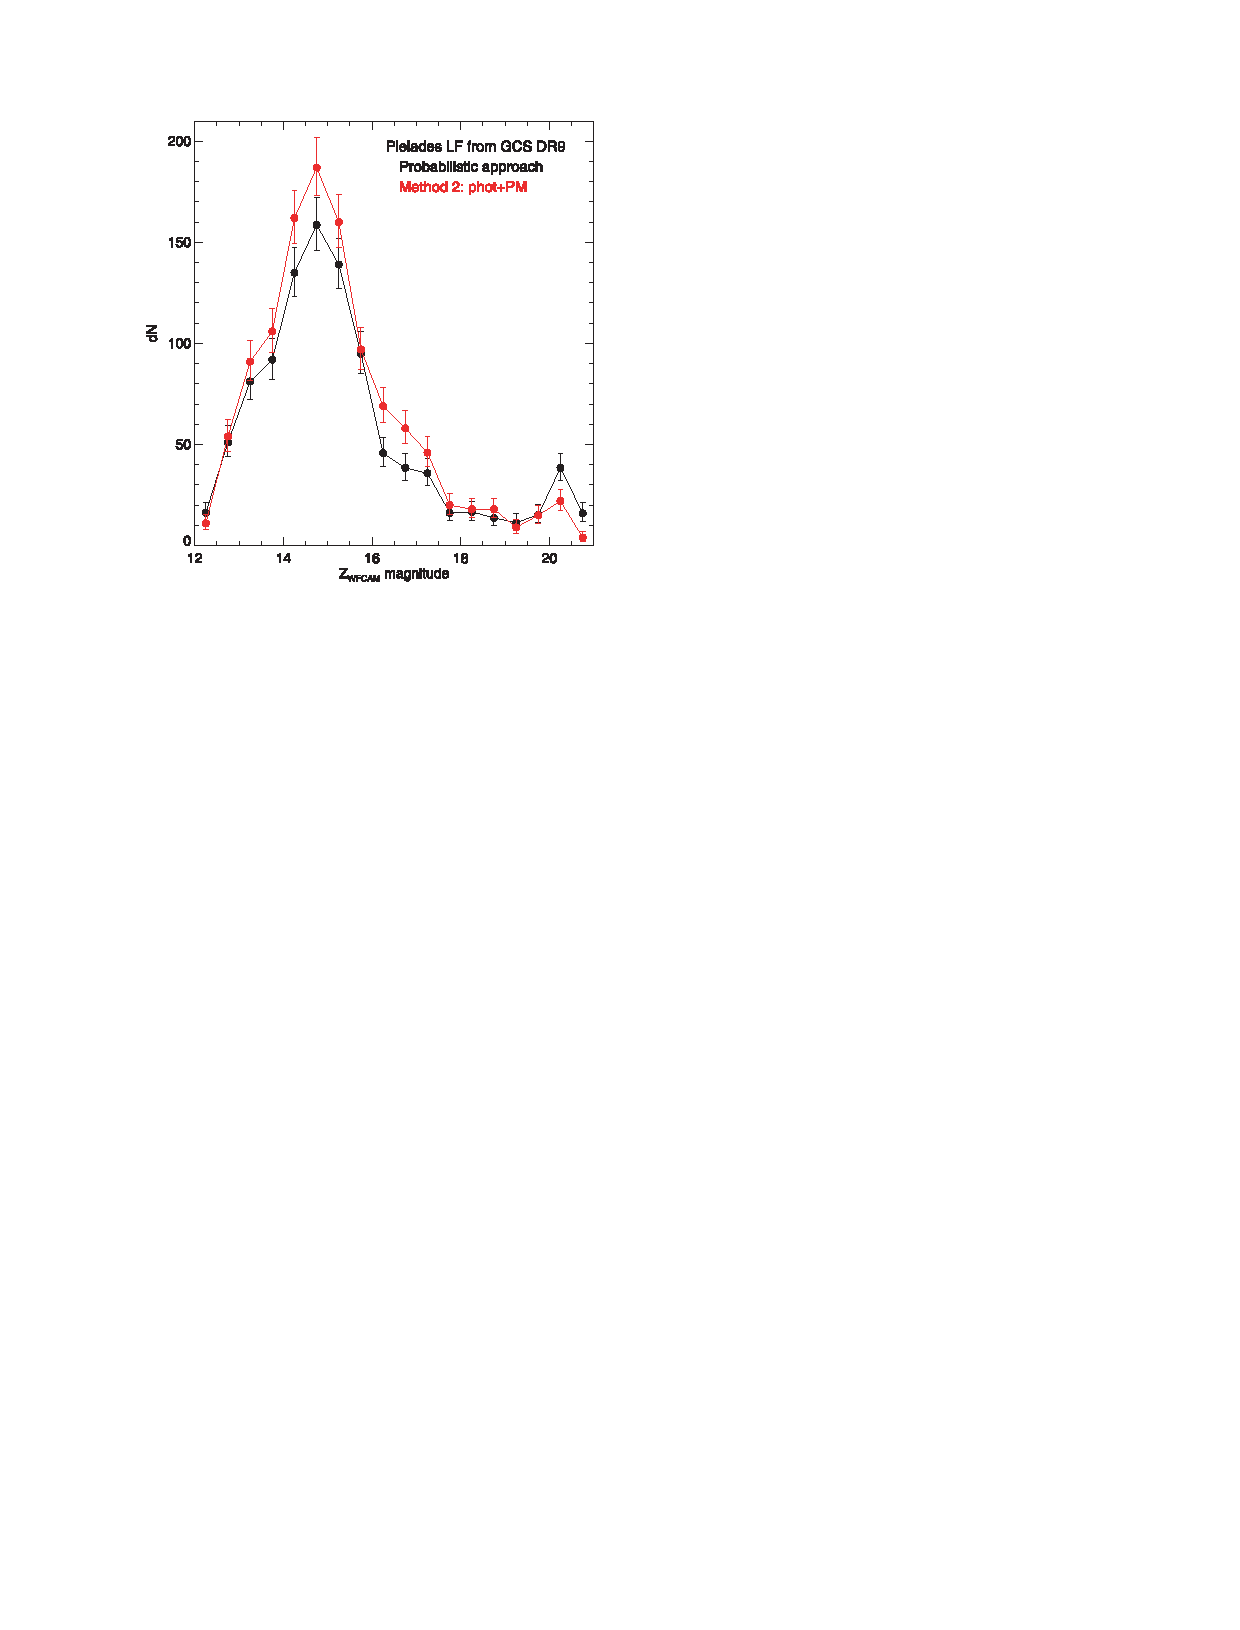
\includegraphics[height=8cm]{background/Figures/F9_Lodieu2012.pdf}
\caption{Luminosity distribution  in the $Z$ band according to \citet{Lodieu2012}. The red and black lines correspond to the two different probabilistic methods.  Reproduced from Figure 9 of \citet{Lodieu2012},\textit{\usebibentry{Lodieu2012}{Title}}, \usebibentry{Lodieu2012}{Journal}, Vol. \usebibentry{Lodieu2012}{Volume}.}
\label{fig:luminosityLodieu}
\end{center}
\end{figure}

In \citet{Bouy2015},  we estimated the present day system luminosity distribution of 1378 candidate members contained within the central $3^{\circ}$ region (with the centre at R.A.$=03:46:48$ and Dec.$=24:10:17$ J2000.0). It is called systemic because it has not been corrected for unresolved systems. An unresolved system is a group of stars (e.g. binaries) that due to its compactness appears as a single object. This distribution was computed for the $K_s$ band and is sensitive up to $K_s \sim 20$ mag and complete until $K_s \sim 17$ mag. This luminosity distribution is reproduced in Fig. \ref{fig:luminosityBouy}


\begin{figure}[ht!]
\begin{center}
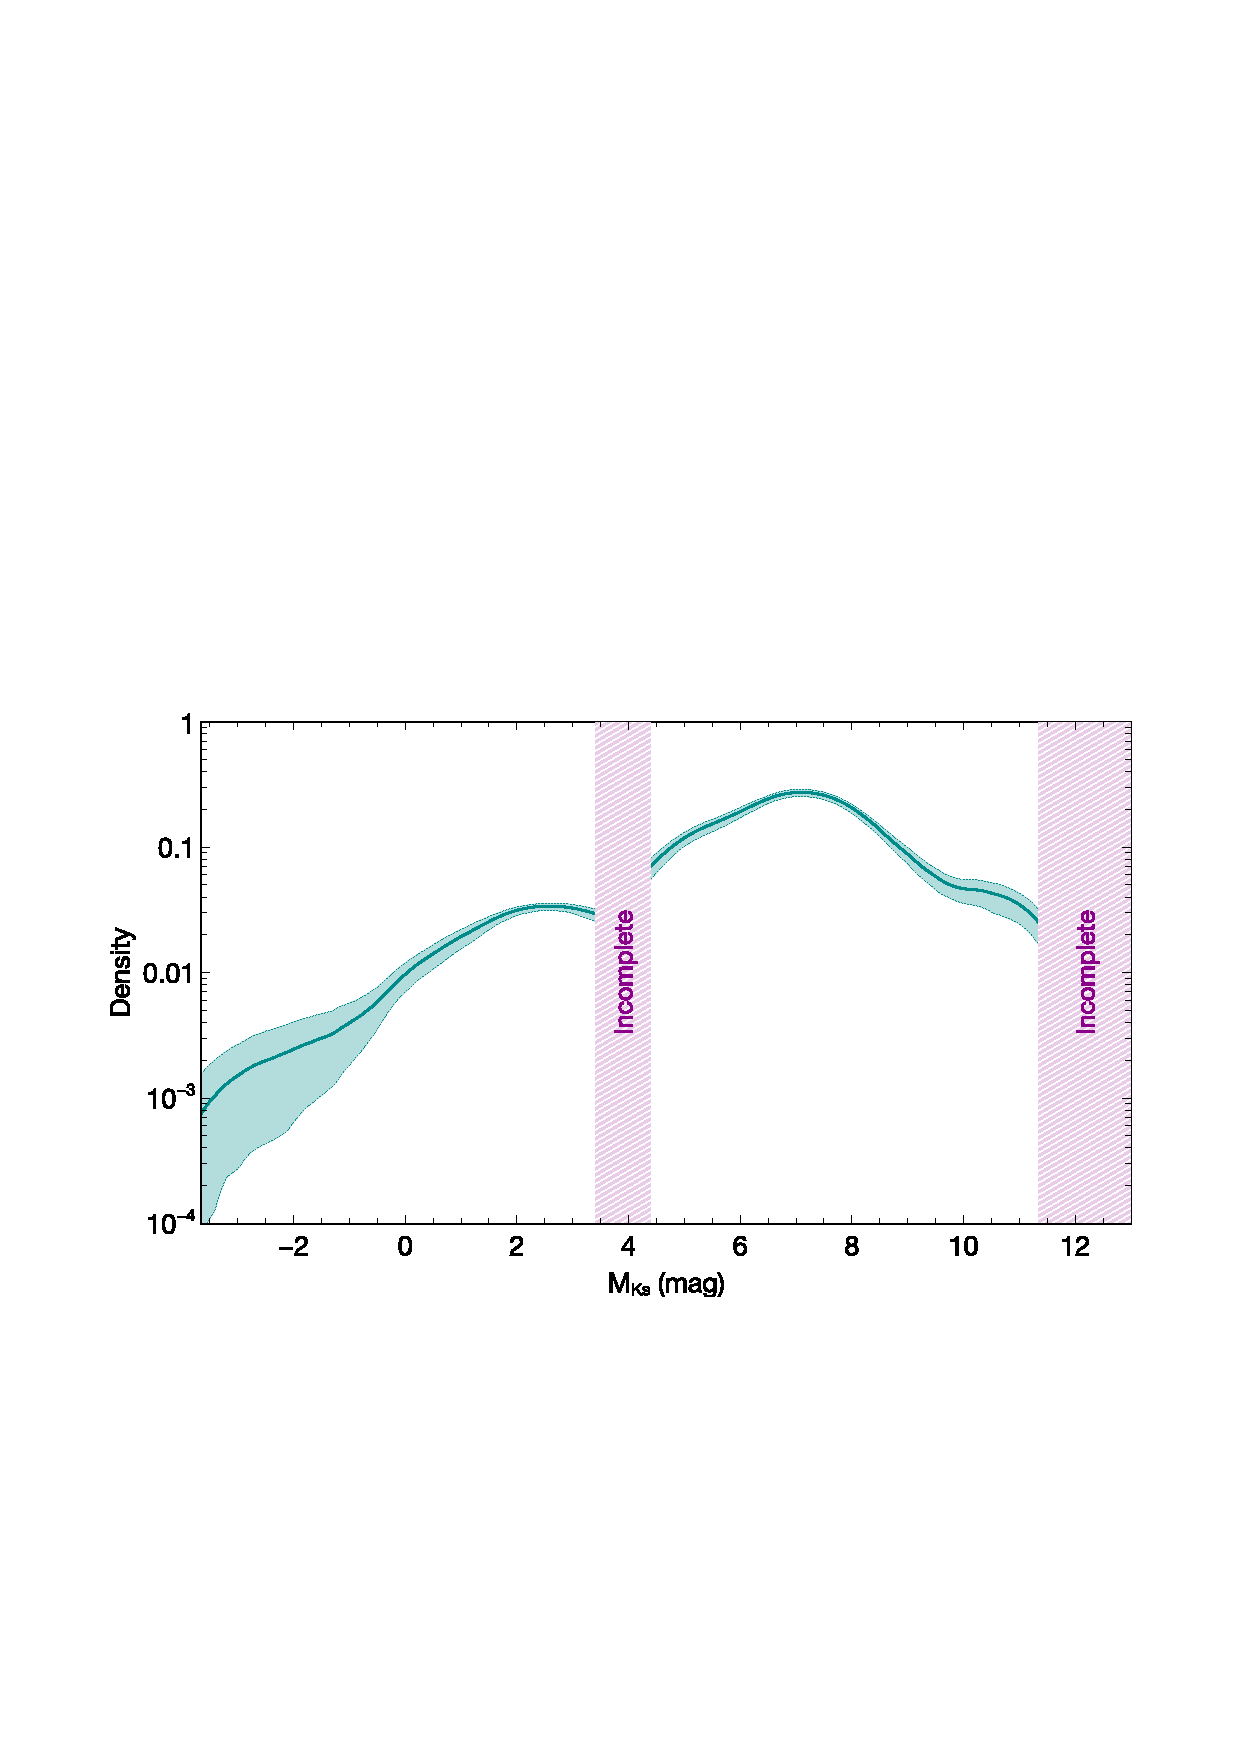
\includegraphics[width=\textwidth]{background/Figures/F8_Bouy2015.pdf}
\caption{Luminosity distribution in the $K_s$ band according to \citet{Bouy2015}. The incompleteness regions are shaded. Reproduced from Figure 8 of \citet{Bouy2015},\textit{\usebibentry{Bouy2015}{Title}}, \usebibentry{Bouy2015}{Journal}, Vol. \usebibentry{Bouy2015}{Volume}.}
\label{fig:luminosityBouy}
\end{center}
\end{figure}

\section{Mass Distribution}
\label{sect:mass}

In astrophysics, the mass distribution is a cornerstone in the understanding of the star formation process and the later evolution of stellar systems. Although the temporal evolution of these systems is mainly dominated by the gravitational potential, the initial conditions and an ongoing star formation process, if any, can contribute to the shape of the mass distribution. This last contains the fingerprints of past events in the history of the cluster and plays a key roll in its future evolution. Indeed, the evolution of the mass distribution is an essential element in one of modern astrophysics' objectives: the determination of the roll played by the initial conditions or the environment, in the temporal evolution of the stellar systems. The mass distribution at the moment of the cluster formation, which is known as the initial mass distribution evolves in time according to: i) stellar internal and atmospheric processes (e.g. contraction, mass loss, inflation, supernova events), ii) population dynamical interactions (e.g. three-body encounters, runaway stars, stellar evaporation), and iii) galactic dynamics (e.g. tidal effects, encounters with other clusters). For these reasons, the study of the initial mass function and its posterior evolution is a key element in the current understanding not just of open clusters but also of galactic and extragalactic populations.  


The mass distribution of the Pleiades has been largely studied. The first work on the mass distribution is that of \citet{Limber1962}. Although he did not show any graphical or tabular representation of it, he gave the luminosity distribution and the mass-luminosity ratio. Form these the mass distributions can be derived. Instead, he use them to obtain the total mass of the cluster ($760\,\mathrm{M_{\odot}}$, see next Section). 

Most probably, the first work to present the mass distribution derived from luminosity distributions and a mass-luminosity relation from theoretical models was that of \citet{Hambly1991}. Using $R$ and $I$ observations from the \emph{United Kingdom Schmidt Telescope Unit} together with the mass-luminosity relation from theoretical isochrone models of Padova group, he was able to transform his luminosity distribution into a mass distribution. In Fig. \ref{fig:massHambly}, I reproduce his results. 

\begin{figure}[ht!]
\begin{center}
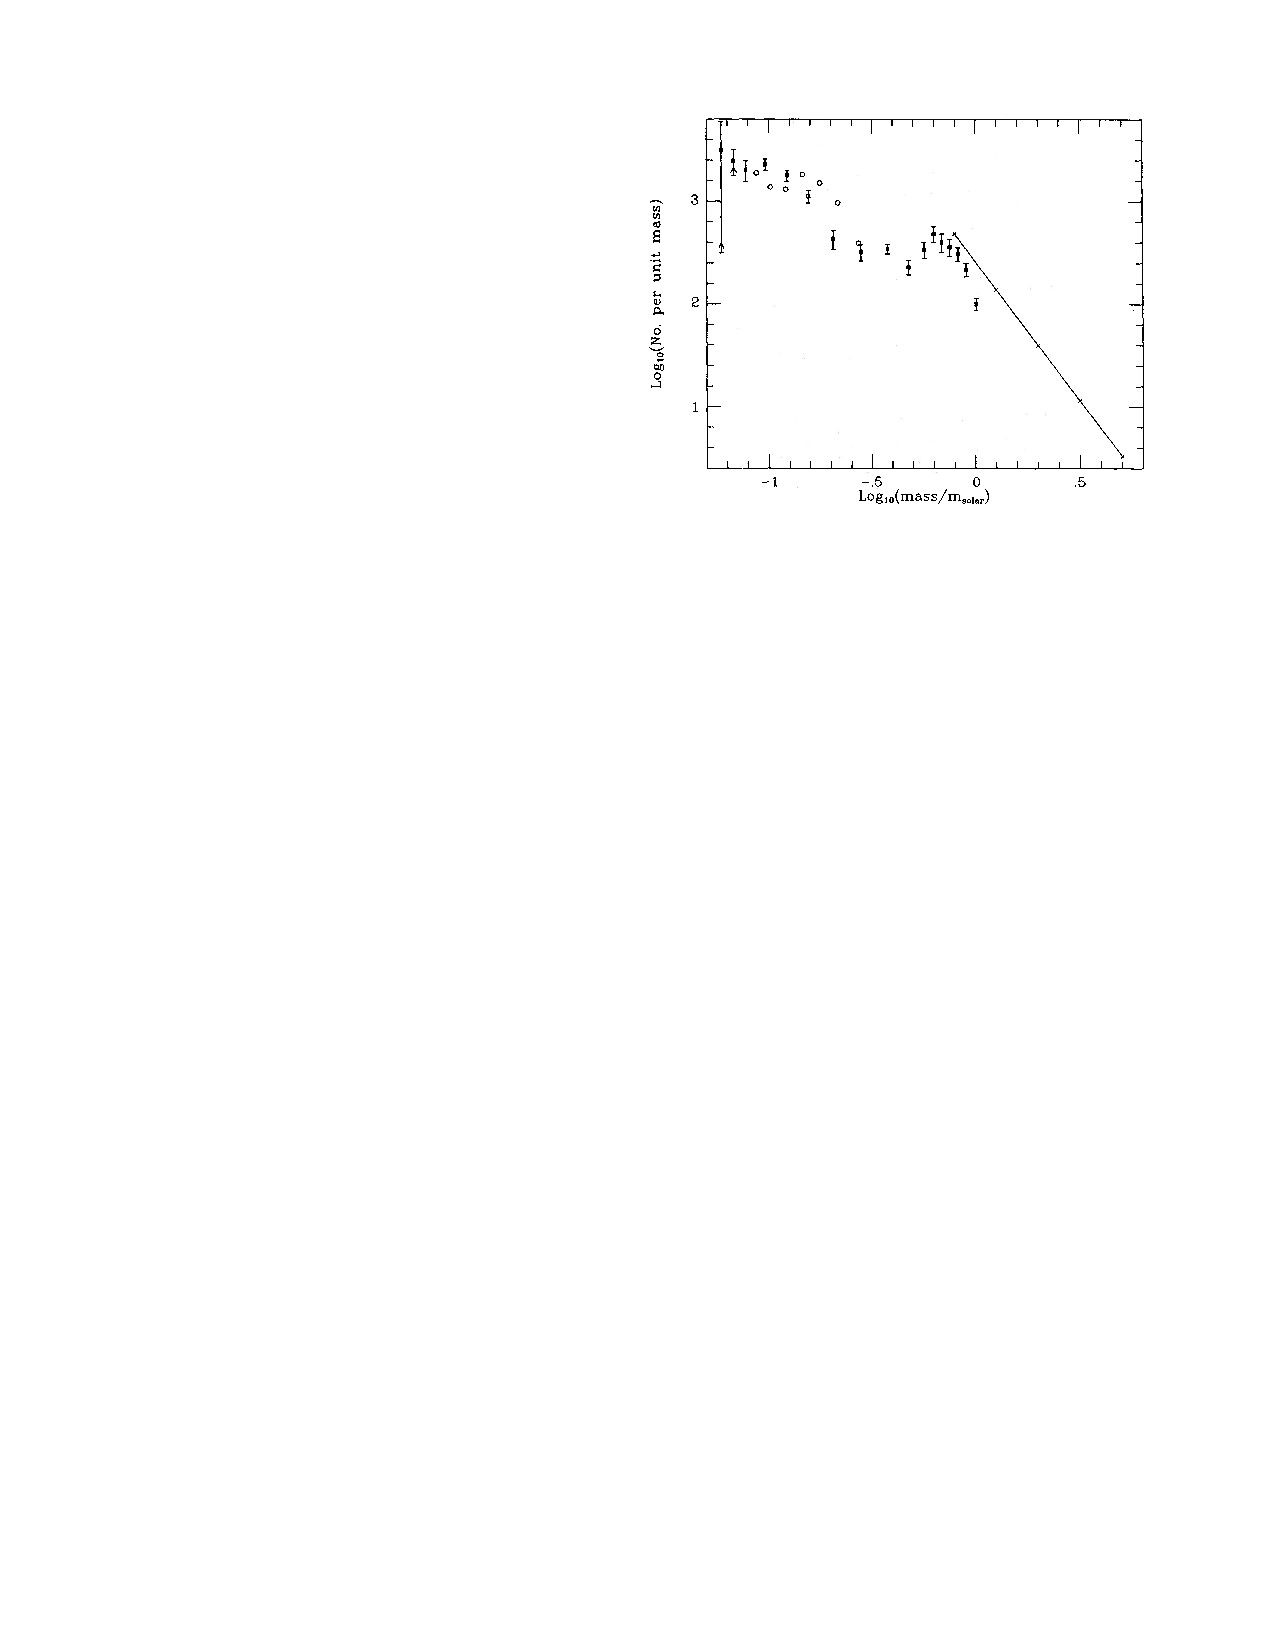
\includegraphics[height=8cm]{background/Figures/F11_Hambly1991.pdf}
\caption{Mass distribution of \citet{Hambly1991} derived from luminosity distribution and theoretical isochrone models. The open circles result from assuming an older age of 200 \gls{myr}. The line represent the mass distribution of \citet{1980IAUS...85..157V}. Reproduced from Figure 11 of \citet{Hambly1991},\textit{\usebibentry{Hambly1991}{Title}}, \usebibentry{Hambly1991}{Journal}, Vol. \usebibentry{Hambly1991}{Volume}.}
\label{fig:massHambly}
\end{center}
\end{figure}

From the year 2000 till date, several studies have been published in which the subject of analysis is the Pleiades mass distribution, e.g. \citet{2000ASPC..198...59H, 2002MNRAS.335..853J, 2001A&A...367..211M,2003A&A...400..891M, 2004A&A...426...75M, 2007MNRAS.380..712L}. However, for the sake of simplicity, here I only analyse the two most recent works, those of \citet{Lodieu2012} and \citet{Bouy2015}. The \gls{pdsmd} derived from both these works are shown in Figs. \ref{fig:massLodieu} and \ref{fig:massBouy}. These works obtained first the luminosity distribution, and then transformed it into a mass distributions using mass-luminosity relations of theoretical isochrone models. 

\citet{Lodieu2012} used a distance of 120.2 pc, an age of 120 \gls{myr}, and the \emph{NEXTGEN} theoretical models of \citet{1998A&A...337..403B} to transform the luminosity into the mass distribution. On the other hand, in \citet{Bouy2015} we use a distance of 136.2 pc an age of 120 \gls{myr} and the \emph{BT-Settl} theoretical isochrone models of \citet{2014IAUS..299..271A}. 

Both works found that their derived \gls{pdsmd} are in general agreement with the \gls{imf} of \citet{Chabrier2005} for unresolved systems (see Section \ref{sect:IMF}). However, in \citet{Bouy2015} we pointed out that, assuming that the theoretical mass-luminosity relation is correct, the \glspl{imf} of \citet{Chabrier2005} and \citet{Thies2007} predict too many low-mass stars and brown dwarfs in the range $0.04-0.1\,\mathrm{M_{\odot}}$. 

The differences at the low mass regime between the \gls{pdsmd} derived by \citet{Lodieu2012} and \citet{Bouy2015} (see Figs. \ref{fig:massLodieu} and \ref{fig:massBouy}) could arise from the different i) samples of members, ii) mass-luminosity relations, and iii) distances adopted by both works.

The different distances can introduce a general shift in the luminosity, which in turn can shift the mass distribution. This shift in luminosity, however, can be neglected due to its small value, $0.06$ mag.

Concerning the differences between the mass-luminosity relations of the two isochrone models, \citet{2013MmSAI..84.1053A} show that there are clear differences between the effective temperatures delivered by the \emph{BT-Settl} and the \emph{NEXTGEN} models in the low-mass regime, at $5$ Gyr particularly. {However, they do not discuss how this difference change in younger ages. Thus, this effect can not be discarded as the source of the differences.}

Concerning the differences between the lists of candidate members, \citet{Lodieu2012} do not provide (at least explicitly) any estimate of contamination rate of their samples. Furthermore, their membership methodology has some draw backs \cite[see][]{Sarro2014} that may have biased their results. {Therefore, the agreement that \citet{Lodieu2012} found between their present day mass distribution and the \gls{imf} of \citet{Chabrier2005}, which models the field mass distribution, may be an indication that their sample of candidate members is contaminated by the field.  }

On the other hand, in \citet{Bouy2015} we estimated a contamination rate of 7\%. However, we have no evidence for it to be non-homogeneous in mass. Even if the 7\% contaminants were not homogeneously distributed in the mass range, this value is not able to account for the observed discrepancies ($30-40\%$ in the low-mass regime) between the \gls{imf} of \citet{Chabrier2005} and our present day mass distribution.

The previous studies show that there is still work to do in the analysis of the Pleiades mass distribution, particularly at the low-mass regime where the \glspl{imf} show discrepancies with the observed present day mass distribution.  

\begin{figure}[ht!]
\begin{center}
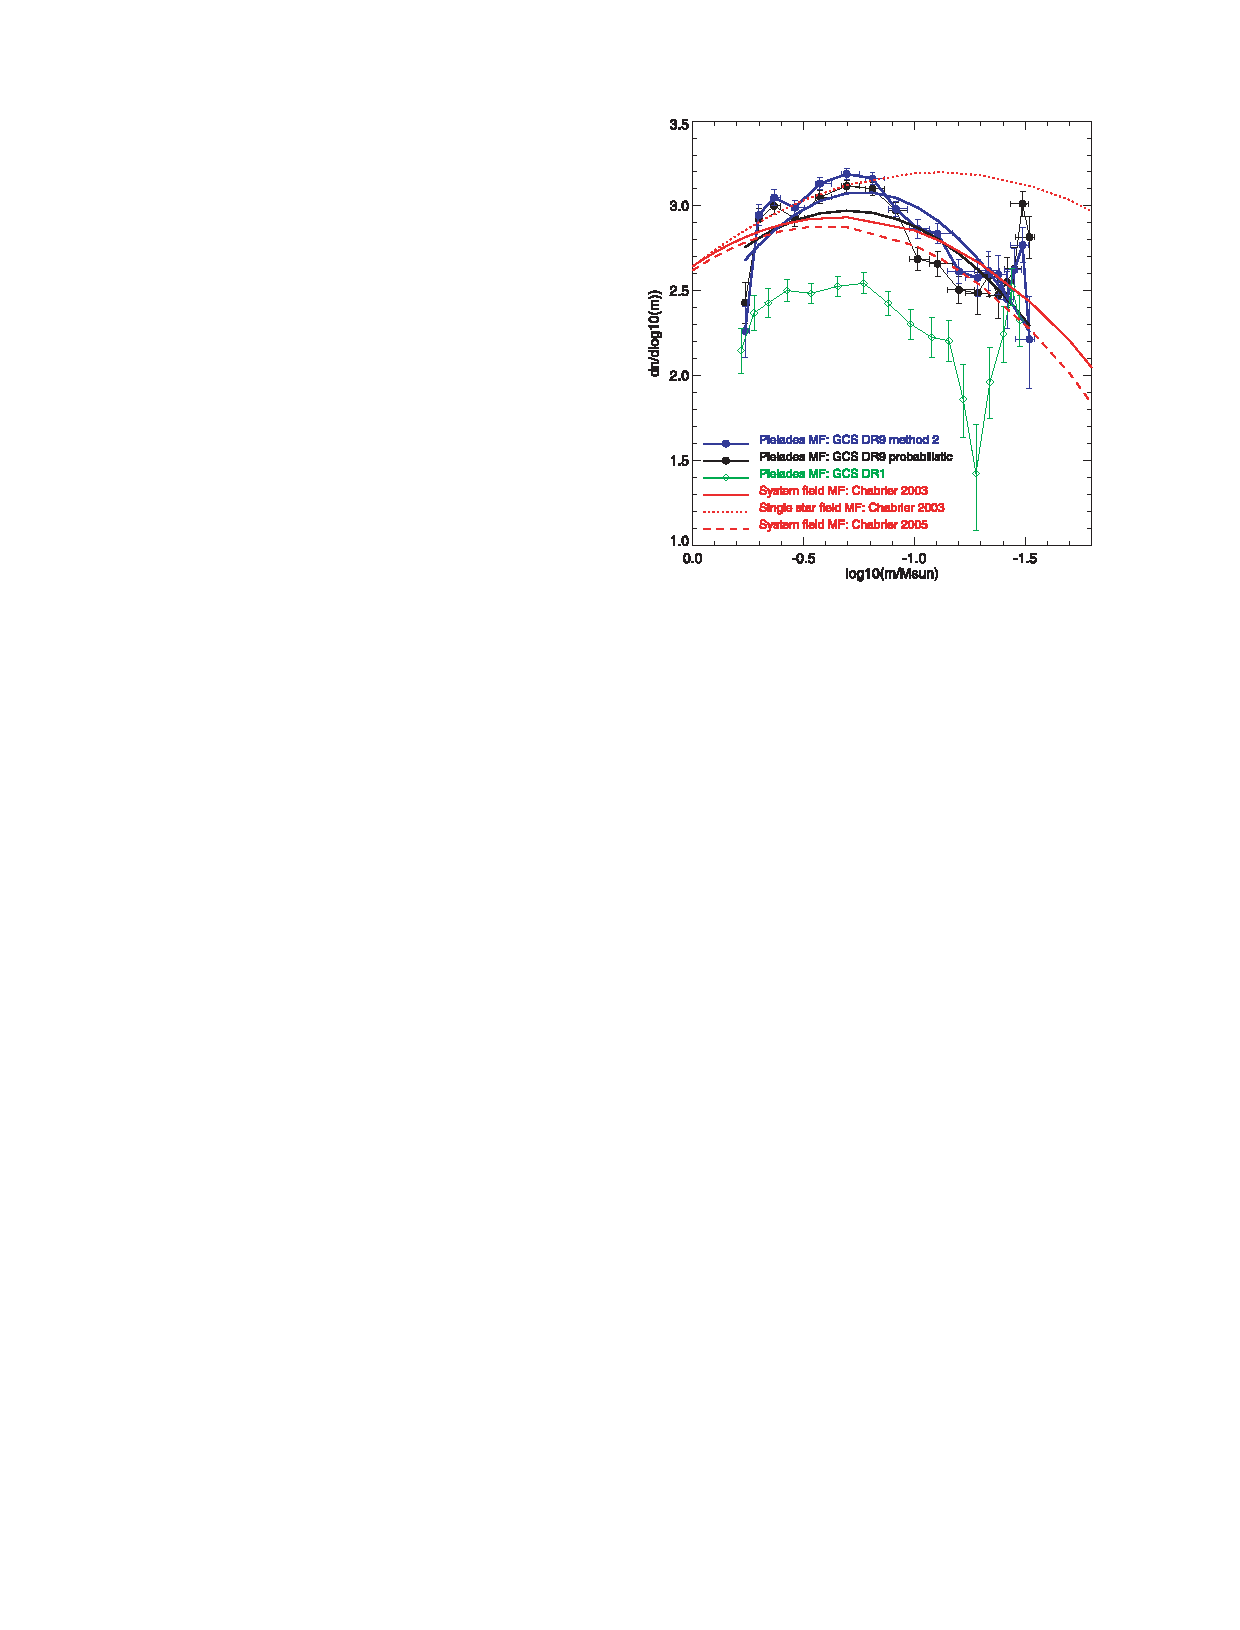
\includegraphics[height=8cm]{background/Figures/F9b_Lodieu2012.pdf}
\caption{Pleiades present day mass distribution from \citet{Lodieu2012}. GCS stands for Galactic Cluster Survey. The first and last two points must be treated with caution due to saturation and contamination at the bright and faint ends, respectively. Reproduced from Figure 9 of \citet{Lodieu2012}, \textit{\usebibentry{Lodieu2012}{Title}}, \usebibentry{Lodieu2012}{Journal}, Vol. \usebibentry{Lodieu2012}{Volume}.}
\label{fig:massLodieu}
\end{center}
\end{figure}

\begin{figure}[ht!]
\begin{center}
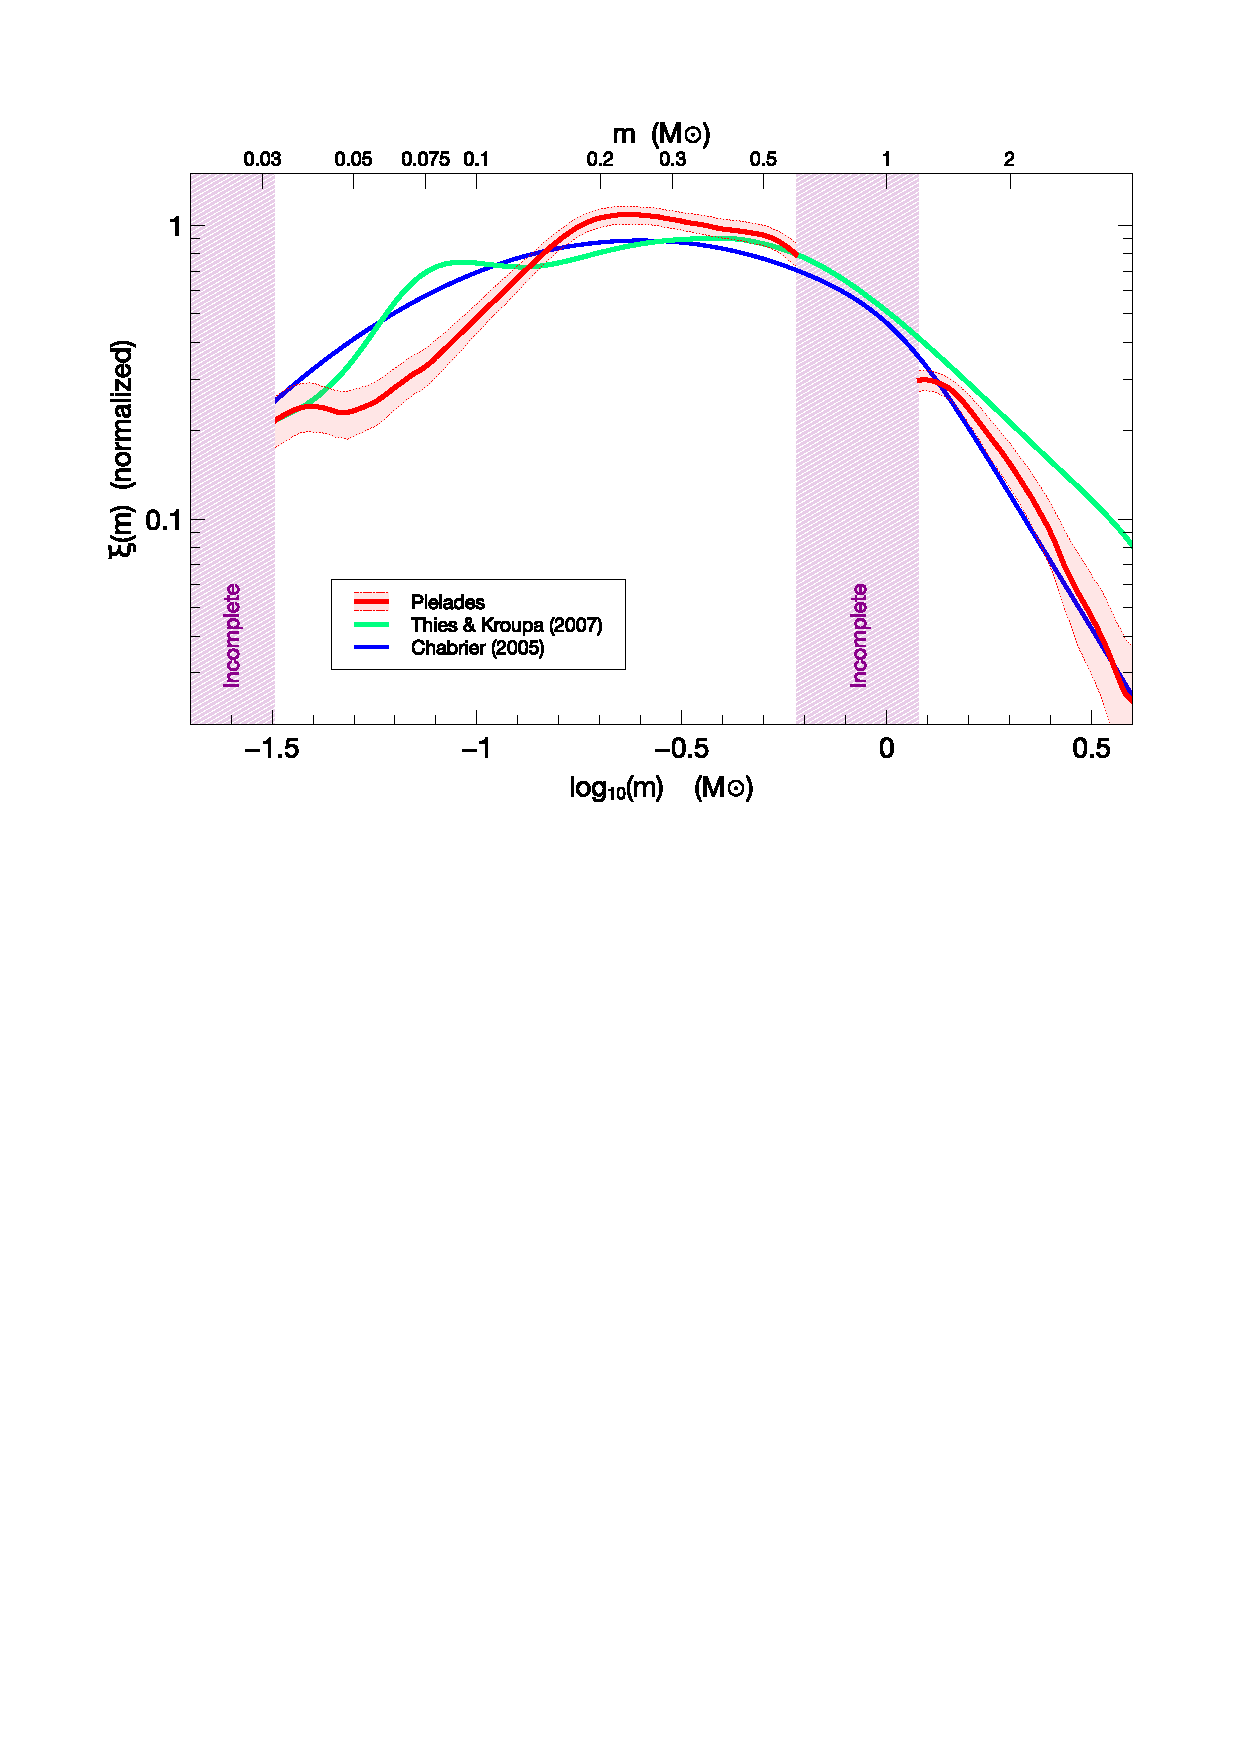
\includegraphics[height=8cm]{background/Figures/F9_Bouy2015.pdf}
\caption{Pleiades present day mass distribution  from \citet{Bouy2015} (red). \glspl{imf} from \citet{Chabrier2005}(blue) and \citet{Thies2007} (green) are also shown. Reproduced from Figure 9 of \citet{Bouy2015}, \textit{\usebibentry{Bouy2015}{Title}}, \usebibentry{Bouy2015}{Journal}, Vol. \usebibentry{Bouy2015}{Volume}.}
\label{fig:massBouy}
\end{center}
\end{figure}

\subsection{Total mass of the cluster}
Before ending this section I present a (non exhaustive) summary of the studies that provided an estimate of the total mass of the cluster.

The first record I found of the cluster total mass is that of \citet{1938AJ.....47...25T}. He estimated a total mass of $260 \,M_{\odot}$ assuming virial equilibrium. He also computed $200 \,\mathrm{M_{\odot}}$ using the Eddignton's mass-luminosity relation for objects brighter than $15$ mag in the visual band.

The subsequent works continue to report higher masses. \citet{1956MNRAS.116..296W} estimated a total mass of $337 \,\mathrm{M_{\odot}}$ using a polytrope model fitted to Hertzsprung's catalogue. He then mentions that taking into account Trumpler's data, the total mass should be about $500\,M_{\odot}$. 

\citet{Limber1962} computed the total mass in two ways. In the first one he assumed the cluster was virialised and obtained a mass of $900 \,M_{\odot}$. Using the luminosity function he estimated the lower limit to the total mass in $760 \,\mathrm{M_{\odot}}$. 

\citet{1970AJ.....75..563J} measured $470\,\mathrm{M_{\odot}}$ and $690\,\mathrm{M_{\odot}}$ using the luminosity distribution and the virial theorem, respectively. 

Later, \citet{1980IAUS...85..157V}  determined a total mass of $2000 \,\mathrm{M_{\odot}}$ using the virial theorem, a mean individual mass of $2\,\mathrm{M_{\odot}}$, and a velocity dispersion of $0.7\,\mathrm{km \cdot s^{-1}}$ in each spatial direction. 

\citet{1995JKAS...28...45L} measured $700 \,\mathrm{M_{\odot}}$ using the luminosity distribution and a mass-luminosity relation. 

\citet{Pinfield1998} fitting a King profile to the \gls{psd} of the cluster members obtained $735\,\mathrm{M_{\odot}}$. 

\citet{Adams2001} counting individual masses of candidate members within $5.5^{\circ}$ obtained a total mass of $690 \,\mathrm{M_{\odot}}$. 

\citet{Converse2008} found $820 \,\mathrm{M_{\odot}}$ after adding the individual masses of 1245  candidate members of \citet{Stauffer2007}. To obtain these masses they  transformed the $K$ and $I-K$ magnitude and colour into masses using the mass-luminosity relation given by the theoretical isochrone models of \citet{1998A&A...337..403B}. Later, \citet{Converse2010} redid their analysis and found the total mass to be $870\pm35\,\mathrm{M_{\odot}}$.

%\section{The current dynamical scenario}
%The most important sources of gravitational interactions affecting individual objects are due to: other individual objects (like for example close encounters or binary interactions), the ensemble of individual objects (the potential of the cluster itself or its momentum), other ensembles of objects (interactions with other clusters or molecular clouds) and, the galactic potential (perturbations due to the disk, resonances, arms).
%
%\subsection{Pleiades time-scales}
%Pinfield equation 13 and 14

\section{The Pleiades DANCe DR2}
\label{sect:DR2}

The \glsfirst{ddr2} contains astrometric (stellar positions and proper motions) and photometric ($ugrizYJHK_s$) measurements for 1,972,245 objects. As explained in Chapter 1, the \gls{dance} data set has an heterogenous origin, which can be observed in Fig. \ref{fig:originDANCeDR2} where the patchy pattern arise from the combination of several surveys. The interested reader can find more the details of this data set and its processing on \citet{Bouy2013}. Here, I briefly summarise its properties. Table \ref{tab:DR2properties} contains the basic statistics for the observables, while Table \ref{tab:DR2uncertainties} does it for the uncertainties. As an example, Fig. \ref{fig:pmuncert} shows the proper motions uncertainties as a function of the $i$ magnitude.

\begin{figure}[ht!]
\begin{center}
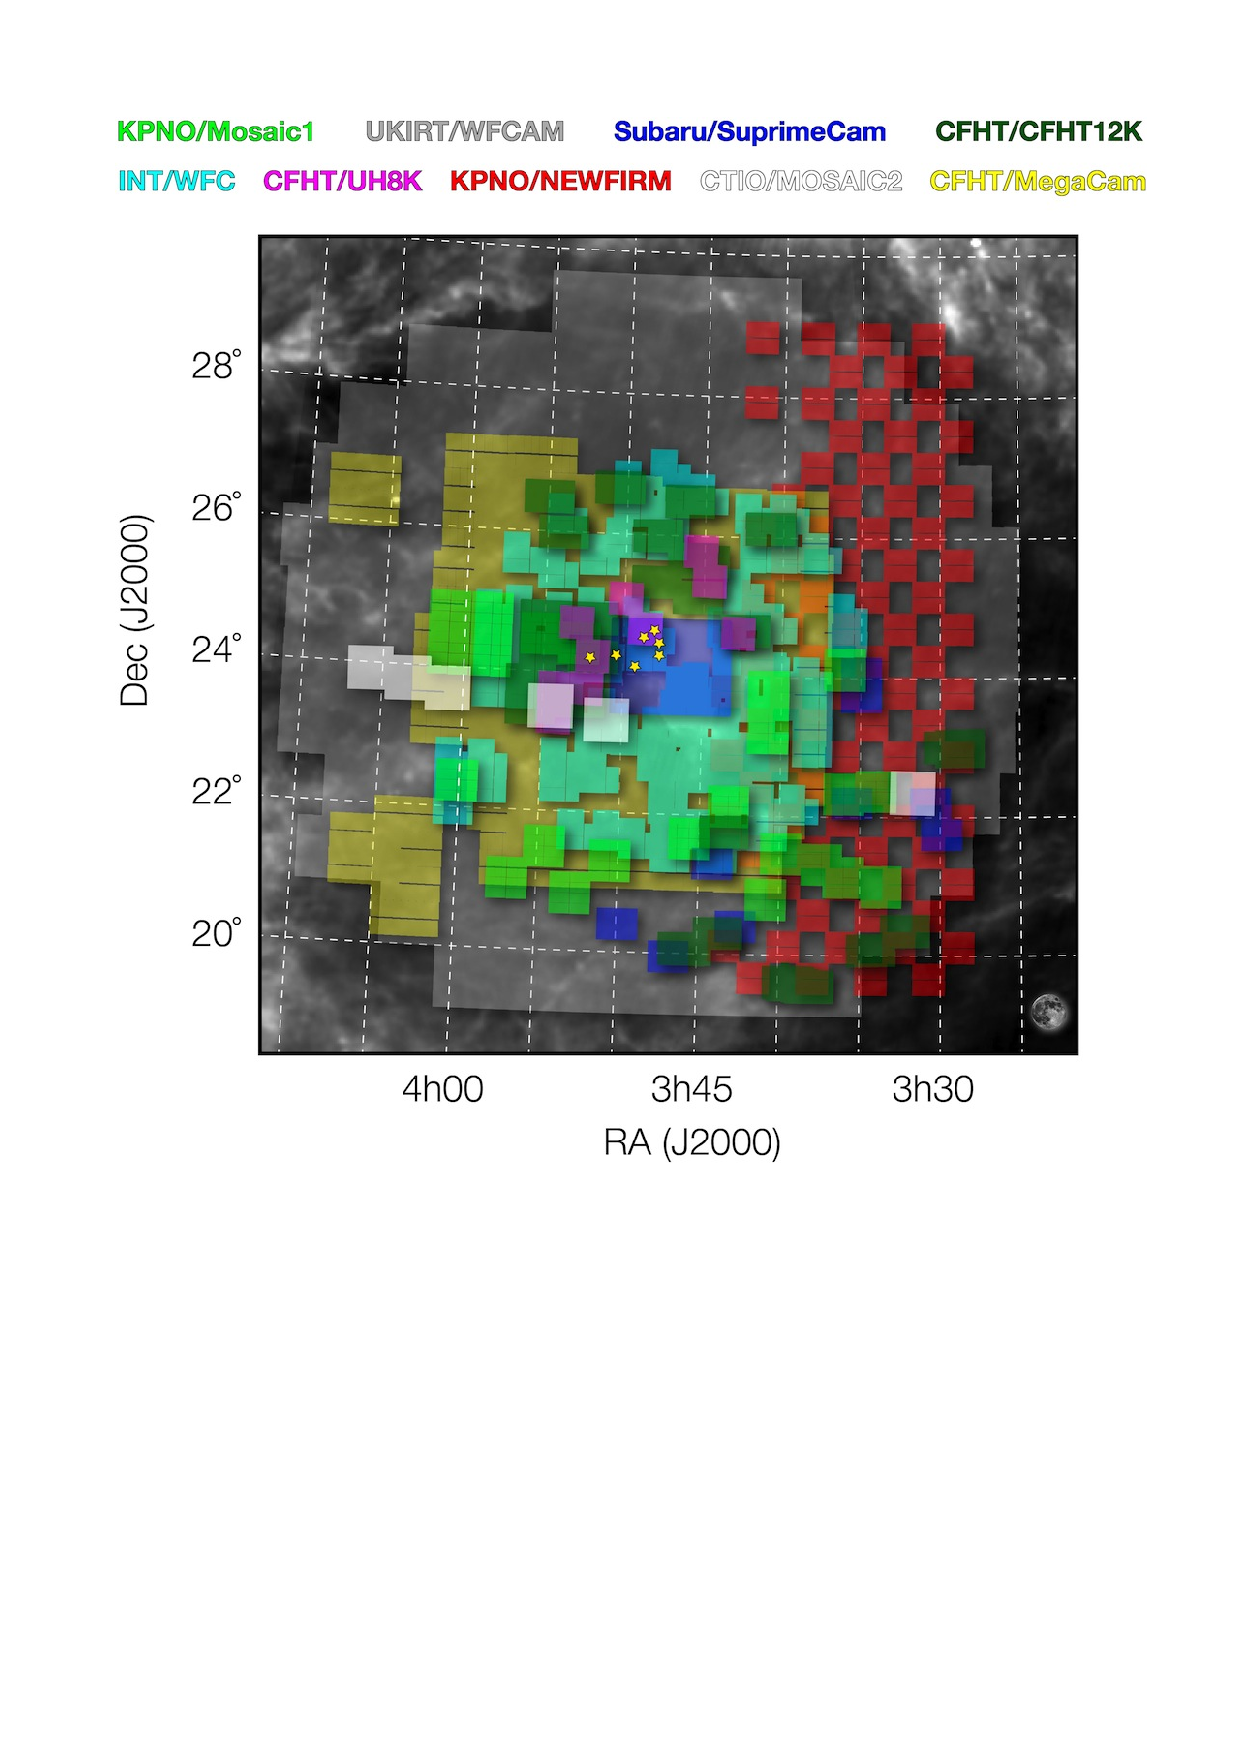
\includegraphics[width=\textwidth]{background/Figures/F1_Bouy2013.pdf}
\caption{Patchy composition of the \gls{ddr2}. The moon shows the scale, and the yellow stars correspond to the central brightest objects of the Pleiades cluster. As can be seen, the UKIDSS (UKIRT) survey provides the most homogeneous and extended coverage. Reproduced from Figure 1 of \citet{Bouy2013}, \textit{\usebibentry{Bouy2013}{Title}}, \usebibentry{Bouy2013}{Journal}, Vol. \usebibentry{Bouy2013}{Volume}.}
\label{fig:originDANCeDR2}
\end{center}
\end{figure}

\begin{table}[htdp]
\caption{Summary of the \gls{ddr2}.}
\begin{center}
\begin{tabular}{|c|c|c|c|c|c|c|c|}
\hline
Observable & Min. & 1st. Qu. & Median & Mean & 3rd. Qu. & Max. & NA's \\
\hline
\hline
RA [deg]&51.23 & 55.40 & 57.35 & 57.26 & 59.01 & 62.94 & 0\\
Dec. [deg] &19.12 &22.47 & 24.32 & 24.27  & 25.95 & 29.69 &0\\
$\mu_{\alpha} [mas\cdot yr^{-1}]$&-99.998& -6.060& -1.645& -1.240&3.401&99.996&0\\
$\mu_{\delta} [mas\cdot yr^{-1}]$&-99.997& -2.835&  2.548&  1.976&  7.017&99.989&0\\
u [mag]&13.6&20.4 &22.0 &21.6&23.3&25.2&1756374\\
g [mag]& 9.4   &19.6   &22.1   &21.1   &23.3   &25.5 &1492564\\
r [mag] &  8.4  &17.6   &21.3   &20.3   &22.6   &25.1   &1222853\\
i [mag] &  7.5  &20.0  &21.6  &21.0  &22.7  &25.5  &820861\\
z [mag]&11.2  &17.9  &19.3  &18.9  &20.2  &25.0  &697412\\
Y [mag]& 8.3  &17.2  &18.5  &18.1  &19.4  &24.2  &688144\\
J [mag]& 2.8  &16.7  &17.9  &17.5  &18.8  &23.1  &645469\\
H [mag]& 2.0  &16.1  &17.3  &16.9  &18.1  &20.9  &653682\\
$K_s$ [mag]& 1.8 &16.0&  17.0  &16.7  &17.7  &23.8  &561745\\
\hline
\end{tabular}
\end{center}
\label{tab:DR2properties}
\end{table}%

\begin{table}[ht!]
\caption{Uncertainties of the \gls{ddr2}.}
\begin{center}
\begin{tabular}{|c|c|c|c|c|c|c|c|}
\hline
Observable & Min. & 1st. Qu. & Median & 3rd. Qu. & Max. &Mean\\
\hline
\hline
RA [deg]&8.900e-08 &9.270e-07&1.933e-06&4.037e-06&2.156e-02&3.173e-06\\
Dec. [deg] &8.900e-08&9.270e-07&1.932e-06&4.037e-06&2.156e-02&3.173e-06\\
$\mu_{\alpha} [mas\cdot yr^{-1}]$&2.01e-01 &1.89e+00& 4.35e+00& 1.00e+01& 1.49e+22&3.99e+16\\ 
$\mu_{\delta} [mas\cdot yr^{-1}]$&1.92e-01 &1.89e+00 &4.35e+00 &1.00e+01 & 4.71e+09&1.42e+04\\
u [mag] &3.73e-04& 8.07e-03& 3.06e-02& 8.56e-02& 2.17e-01&5.48e-02\\
g [mag] &1.72e-01 & 1.02e-02&  3.90e-02 & 7.90e-02 & 1.82e+00&5.34e-02\\
r [mag] & 2.83e-04 & 1.54e-02& 4.88e-02 &1.04e-01& 1.42e+00&6.34e-02\\
i [mag] & 4.04e-04 & 9.03e-03&  2.73e-02& 5.85e-02& 2.40e+00&4.37e-02\\
z [mag] & 6.49e-04& 5.62e-02& 9.16e-02& 1.85e-01& 3.12e+00&1.34e-01\\
Y [mag] & 3.00e-02& 5.21e-02& 6.50e-02& 1.03e-01& 9.01e+00&8.56e-02\\
J [mag] & 1.60e-02& 5.24e-02& 6.66e-02& 1.04e-01& 8.89e+00&8.57e-02\\
H [mag] & 1.40e-02& 5.28e-02& 7.04e-02& 1.10e-01& 1.00e+01&8.85e-02\\
$K_s$[mag]&1.40e-02& 5.75e-02& 8.17e-02& 1.32e-01& 3.88e+01&1.04e-01\\
\hline
\end{tabular}
\end{center}
\label{tab:DR2uncertainties}
\end{table}%

\begin{figure}[ht!]
\begin{center}
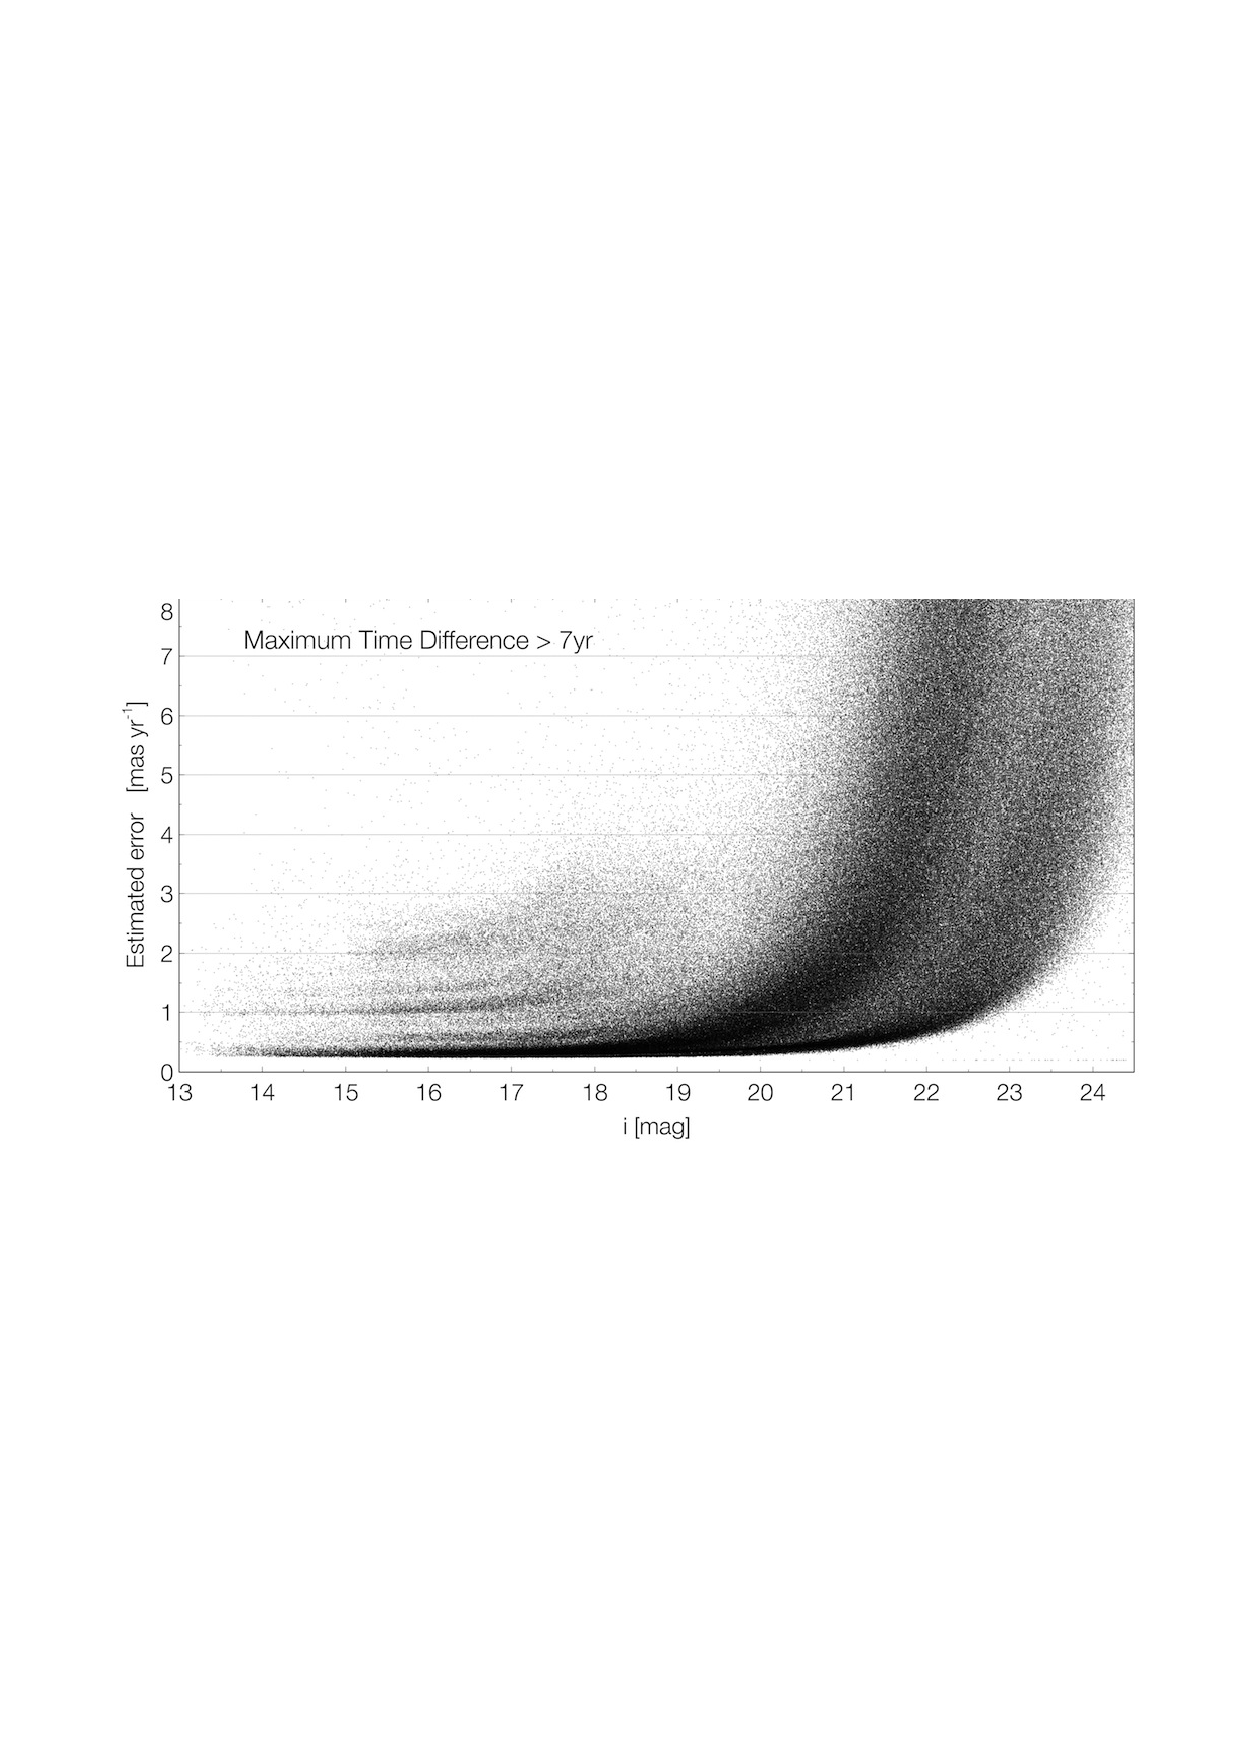
\includegraphics[height=8cm]{background/Figures/F12_Bouy2013.pdf}
\caption{Proper motion uncertainty as a function of the photometric magnitude in the $i$ band. Reproduced from Figure 12 of \citet{Bouy2013}, \textit{\usebibentry{Bouy2013}{Title}}, \usebibentry{Bouy2013}{Journal}, Vol. \usebibentry{Bouy2013}{Volume}.}
\label{fig:pmuncert}
\end{center}
\end{figure}

\subsection{Missing values}
\textbf{In the \gls{ddr2}, missing values occur only in the photometric measurements (see Table \ref{tab:DR2properties}), with the bluer bands being the most affected. As expected, the probability distribution of sources with missing values is not uniform. Missing values occur with higher probability at the faintest end of the photometric distributions ($\sim 18$ mag in $J,H$ and $K_s$ bands). Figure \ref{fig:NAsDDR2} shows the distribution of objects having at least a missing entry as a function of the band or bands that were actually observed. As mentioned, the vast majority of these objects occur at the faint end, close to the sensitivity limit of the survey. It coincides with the sensitivity limits of the UKIDSS Galactic Cluster Survey \cite[$Y\sim 20.3$, $J\sim19.5$, $H\sim K_s\sim18.6$ according to][]{2007MNRAS.379.1599L}, which provides the deepest photometry in the \gls{ddr2}. In this Figure, the bumps at the bright and middle ranges arise due to the mixing of surveys. The first bump corresponds to the survey carried out by \citet{Bouy2015}. As mentioned in their Appendix A, due to saturation, the $Y$ band photometry was limited to objects fainter than $\sim 13$ magnitude. Thus, they complemented the Pleiades \gls{dance} catalogue with shallow $Y$ band photometry in the magnitude range of 8 to 14 magnitudes but only for 40 candidate members of \citet{Stauffer2007} and their surrounding objects \cite[see][for more details]{Bouy2015}. Thus, the large amount of missing $Y$ values in the 8 to 14 mag range of Fig. \ref{fig:NAsDDR2} come from those objects not observed by these authors. The second bump at the middle range is slightly fainter than the sensitivity limits of the 2MASS survey ($J\sim 16.4$, $H\sim15.5$ and $K_s \sim 14.8$, see Section 6.2 of the Explanatory Supplement to the 2MASS All Sky Data Release\footnote{\url{https://www.ipac.caltech.edu/2mass/releases/allsky/doc/sec6_2.html}}), which indicates that it comes from the mixing of the 2MASS and UKIDSS surveys. Due to the different spatial resolutions, some objects are detected in 2MASS and not in UKIDSS and vice versa. The missing $Y$ band values come from objects observed only by 2MASS.}

\begin{figure}[ht!]
    \centering
    \begin{subfigure}[t]{0.45\textwidth}
        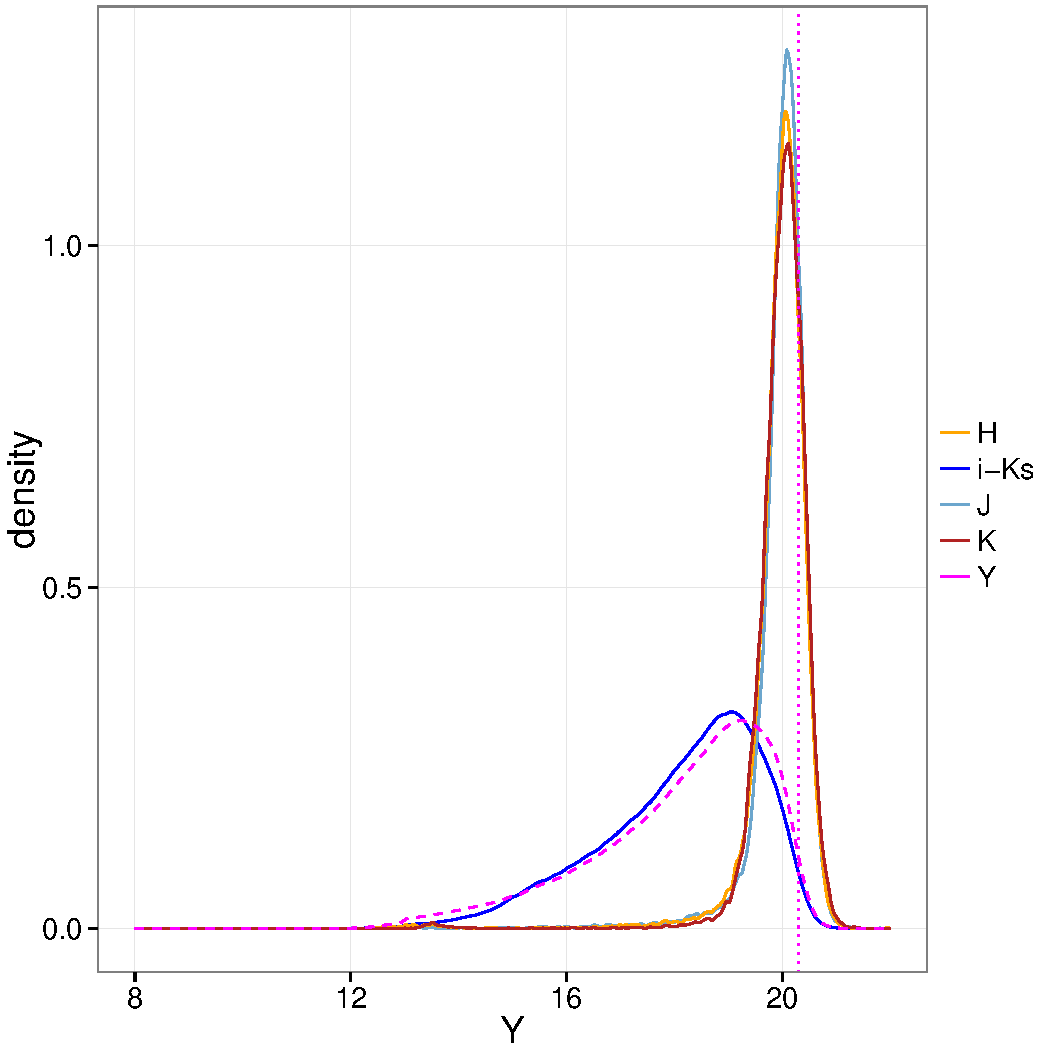
\includegraphics[page=1,height=6cm]{background/Figures/MissingDistributionsDDR2.pdf}
    \end{subfigure}
    \begin{subfigure}[t]{0.45\textwidth}
      \includegraphics[page=2,height=6cm]{background/Figures/MissingDistributionsDDR2.pdf}
    \end{subfigure}
     \begin{subfigure}[t]{0.45\textwidth}
      \includegraphics[page=3,height=6cm]{background/Figures/MissingDistributionsDDR2.pdf}
    \end{subfigure}
     \begin{subfigure}[t]{0.45\textwidth}
      \includegraphics[page=4,height=6cm]{background/Figures/MissingDistributionsDDR2.pdf}
    \end{subfigure}
\caption{Density distributions in $Y,J,H$ and $K_s$ bands for \gls{ddr2} objects with missing values in the other bands. For comparison, the distribution of observed objects is also shown with a dashed line. The majority of the missing value objects are located at the faint end of the magnitude distributions ($Y \sim 20$, $J \sim 19$, $H\sim18.5$, and $K_s \sim 18$). A non negligible fraction of missing  $Y$ band photometry is at the bright end ($J,H,K_s \sim 8 - 14$ mag), and in the middle range of 13 to 16 magnitudes. See text for details.}
\label{fig:NAsDDR2}
\end{figure}

\begin{figure}[ht!]
    \centering
    \begin{subfigure}[t]{0.45\textwidth}
        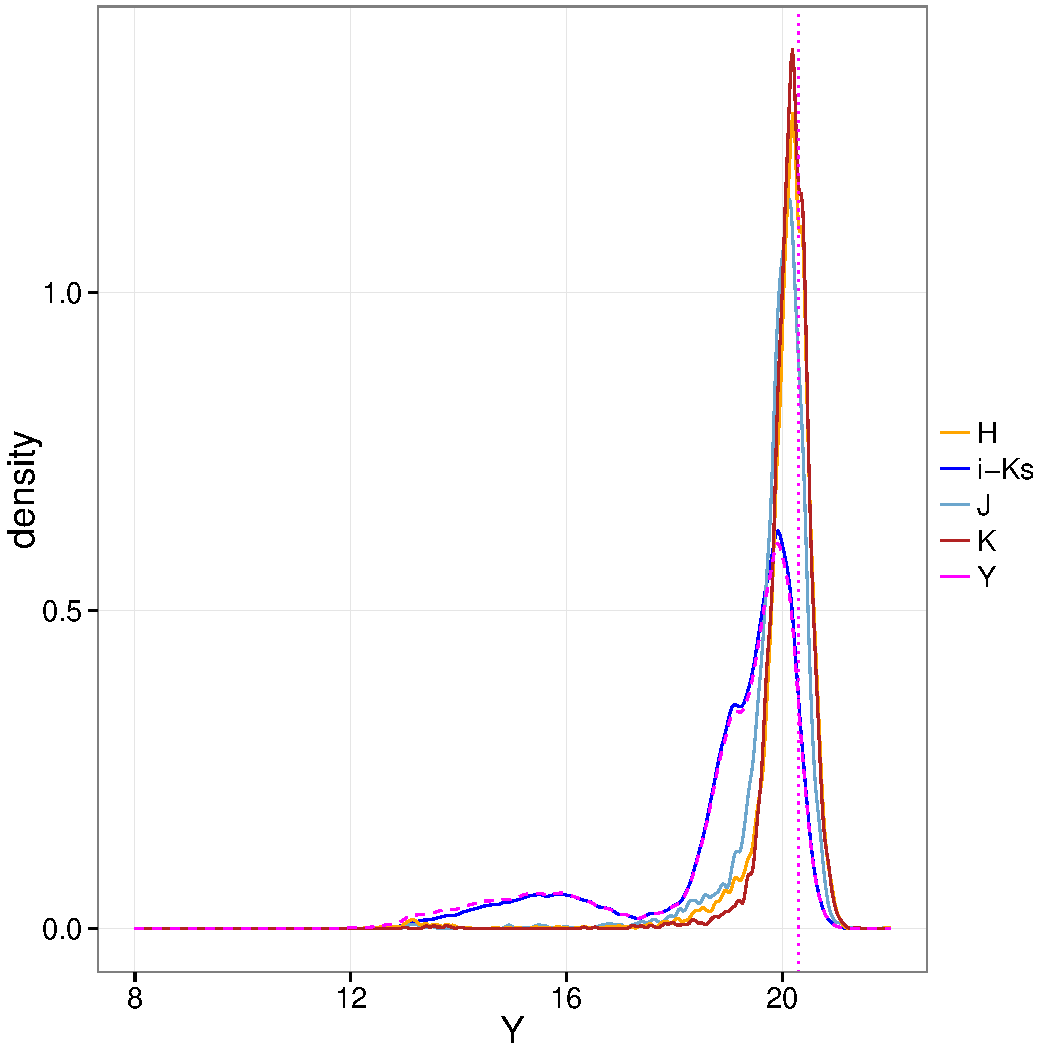
\includegraphics[page=1,height=6cm]{background/Figures/MissingDistributions.pdf}
    \end{subfigure}
    \begin{subfigure}[t]{0.45\textwidth}
      \includegraphics[page=2,height=6cm]{background/Figures/MissingDistributions.pdf}
    \end{subfigure}
     \begin{subfigure}[t]{0.45\textwidth}
      \includegraphics[page=3,height=6cm]{background/Figures/MissingDistributions.pdf}
    \end{subfigure}
     \begin{subfigure}[t]{0.45\textwidth}
      \includegraphics[page=4,height=6cm]{background/Figures/MissingDistributions.pdf}
    \end{subfigure}
\caption{Density distributions in $Y,J,H$ and $K_s$ bands of \gls{rdr2} for objects with missing values in the other bands. For comparison, the distribution of observed objects is also shown with a dashed line. The features are similar to those in Fig. \ref{fig:NAsDDR2}. The small differences between the two figures come from the fact that the \gls{rdr2} is not a random sample of the \gls{ddr2}.}
\label{fig:NAs}
\end{figure}

\subsection{Selection of observables}
\label{sect:RF-2}
\sloppy
The \gls{ddr2} contains the positions R.A., Dec. (in the following $\alpha$ and $\delta$), proper motions, $\mu_{\rm{R.A.}},\mu_{\rm{Dec.}}$, and photometric $ugrizYJHK_s$ bands, of almost two million sources on the vicinity of the Pleiades clusters. Although these 13 observables carry information valuable to discriminate cluster members from field objects, not all of them do it in the same way. A detailed analysis of the capacity of the previous set of observables (except the stellar postions) to discriminate between cluster members and field population is present in the work of \citet{Sarro2014}. These authors use random forest to select the observables that were the most discriminant. They find that the observables of  proper motions ($\mu_{R.A.},\mu_{Dec.}$) and the photometric bands $rizYJHK_s$ are the most discriminants. 

However, since most the objects with a missing $r$ band occur at the faint end of the cluster sequence, \citet{Sarro2014} train their model in two stages. In the first stage, they use all literature candidate members with observed $r$ band. In the second stage, they discard the $r$ band observations and continue training their model with objects in which the $r$ band was missing.  In a subsequent analysis using roughly the same methodology, \citet{Bouy2015} skipped the first training stage and worked only with the RF-2, which also excludes the $z$ band.

Therefore, in the present work I use as a reference set the the proper motions, $\mu_{\alpha},\mu_{\delta}$, the photometric bands $Y,J,H,K_s$, and the colour index $i-K_s$, with the addition of the stellar positions  $\alpha$ and $\delta$. This decision roots in two key aspects. First,  \citet{Sarro2014} prove that this observables (excluding the stellar positions) are amongst the most discriminant ones. Second, this set corresponds to the one used by \cite{Bouy2015}, thus, it will enable us to perform a direct comparison and validation with their results. 

However, there is a subtle difference between the set of observables used by \cite{Bouy2015} and the ones use in the present work. While here I use the $Y$ band alone, \citet{Bouy2015} use the colour index $Y-J$. Originally, I tested the methodology with this $Y-J$ colour index, however, the contamination resulting from the use of the $Y$ gets reduced with respect to that of the $Y-J$ colour index. I interpret this situation as resulting from at least two points. First, the $Y-J$ colour index does not convey information for the sequence of equal-mass binaries, thus reduces the capacity to identify these objects. Second, the width of the cluster sequence in the $Y-J$ vs. $i-K_s$ colour-colour diagram varies greatly across $i-K_s$ when compared to the relatively stable width of the cluster sequence in the the $Y$ vs $i-K_s$ \gls{cmd}. This effect can be observed in Figure \ref{fig:Y-JvsY}, where the candidate members of \citet{Bouy2015} (blue dots) are depicted, together with the \gls{rdr2} density, in the colour-colour diagram $Y-J$ vs. $i-K_s$, and the  \gls{cmd} $Y$ vs $i-K_s$. Since the current version of the photometric model describes the cluster sequence with a constant width across the $i-K_s$ colour index (details are shown in Section \ref{sect:cluster_ph}), then the use of $Y-J$ results in larger contamination in those regions where the clusters sequence is narrower than the average. Future steps will be take to include more colour indices in the reference set of observables.

\begin{figure}[htp!]
\begin{center}
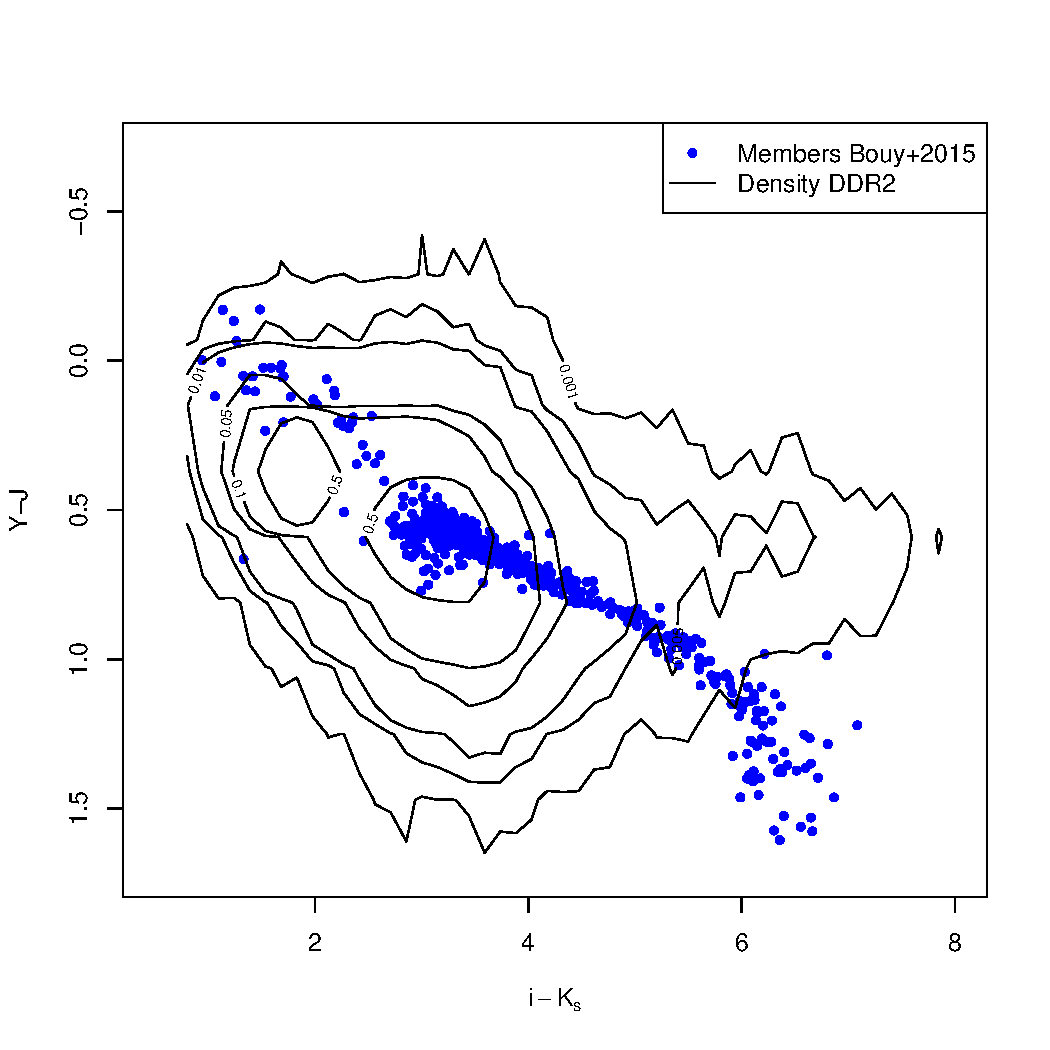
\includegraphics[page=1,width=0.47\textwidth]{background/Figures/Y-J.pdf}
\includegraphics[page=2,width=0.47\textwidth]{background/Figures/Y-J.pdf}
\caption{Candidate members of \citet{Bouy2015}, blue dots, together with the density of the \gls{rdr2} data set, black contours, in the colour-colour  diagram $Y-J$ vs. $i-K_s$ (left) and \gls{cmd} $Y$ vs $i-K_s$ (right).}
\label{fig:Y-JvsY}
\end{center}
\end{figure}
 

 
Concerning the stellar positions $\alpha$ and $\delta$, neither \citet{Bouy2015} nor \citet{Sarro2014} use them in their analyses. Thus, I will independently analyse the: i) the kinematic and photometric distributions of the cluster population, and ii) the \gls{psd}. This decision roots in the following reasons.

First. To fulfil the objective of the \gls{dance} project (see Section \ref{sect:DANCeproject}), the inventory of kinematic and photometric distributions of the \glspl{nyc} must be obtained with an homogenous methodology. The \gls{dance} \gls{nyc} targets (see Tables \ref{tab:maintargets} and \ref{tab:secondarytargets}) do not share similar projected spatial density profiles; while Taurus, Ophiucus and the Trapezium are extended \cite[see for example][]{simon1997}, the Pleiades is almost radially symmetric \citep{Raboud1998}. Thus, including the spatial information together with the proper motions and photometry would require completely different models for the \gls{psd} of different clusters. That would result in non-homogenous methodologies that would bias any comparison between the derived \gls{pdsmd} of these clusters.

{Second. To validate the results of the present work, which will be conducted in the Pleiades cluster, we must compare them with similar results under the most similar conditions. Since \citet{Bouy2015,Sarro2014} do not include the stellar positions in their observables, I do that as well. }

{Third. Almost all previous analyses of the Pleiades \gls{psd} use King profile (see Section \ref{sect:PSD}) without providing any further reason that its physical interpretability, which nevertheless remains a good one. Thus, we decided to perform a Bayesian model selection analysis to compare how well the common surface density profiles, included the King's one, reproduce the Pleiades \gls{psd}. The results of this analysis are in preparation and will be soon submitted to the $A\&A$ journal. }

As will be described in Section \ref{subsect:cluster}, the photometry is modelled by parametric series of cubic splines. I choose the \emph{true} \gls{ci} to be the parameter of these series. This colour allows the most one-to-one dependent-independent variable relations. This one-to-one relation can be seen in Figures \ref{fig:CI} and \ref{fig:otherCI}, where I show the colour-magnitude diagram of $K$ vs $i-K_s$ and $K$ vs colours $Y-K_s$, $J-K_s$, $H-K_s$, and $Y-J$, respectively.  This one-to-one relation is crucial to avoid degeneracies. Without it, two magnitudes could be described by the same colour index. Therefore a monotonic relation would not be valid. 

Thus, our photometric set of observables is made of $i-K_s, Y,J,H$ and $K_s$. 

\begin{figure}[ht!]
\begin{center}
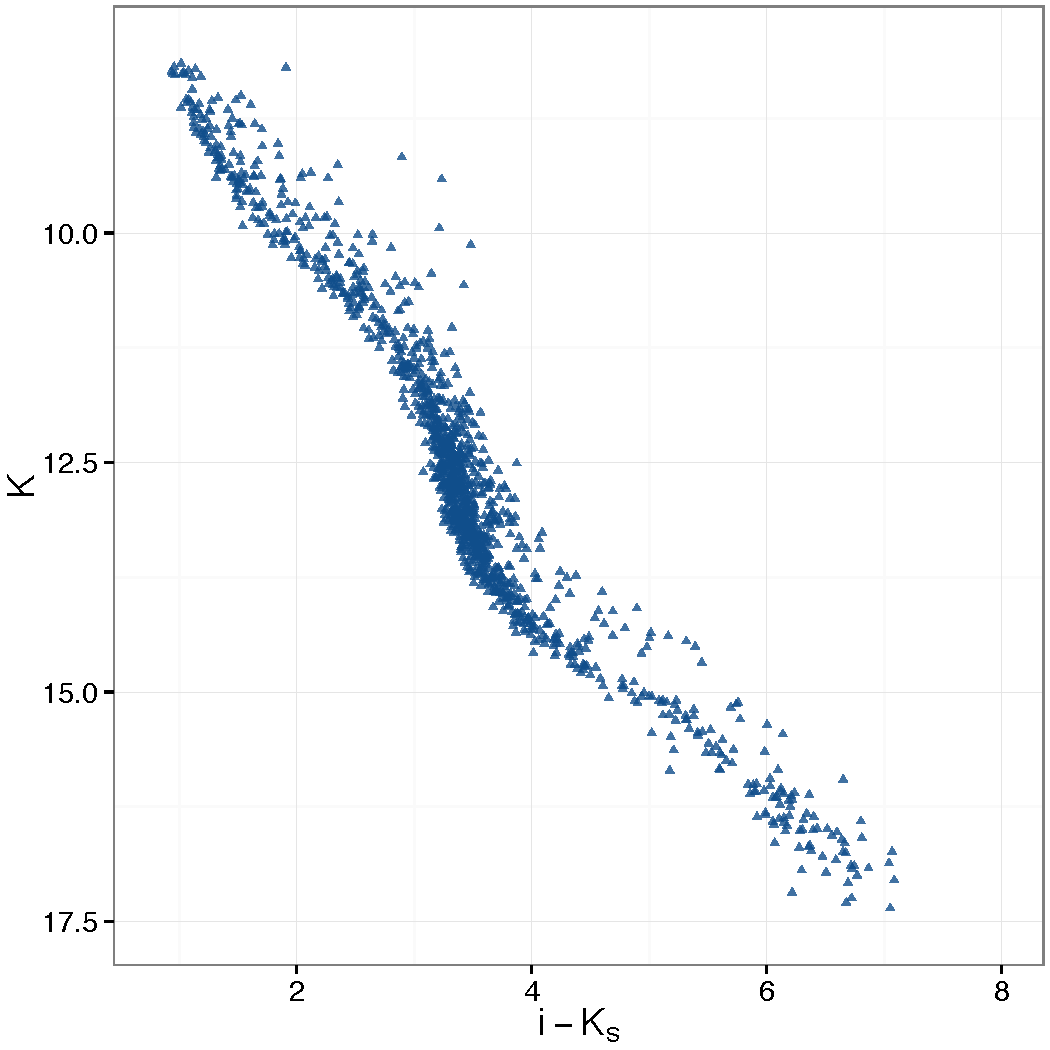
\includegraphics[page=1,height=8cm]{background/Figures/CIs.pdf}
\caption{$K_s$ vs $i-K_s$ CMD for the Pleiades candidate members of \citet{Bouy2015} with membership probability $>0.75$.}
\label{fig:CI}
\end{center}
\end{figure}

\begin{figure}[ht!]
    \centering
    \begin{subfigure}[t]{0.45\textwidth}
        \includegraphics[page=2,height=6cm]{background/Figures/CIs.pdf}
        \caption{}
        
    \end{subfigure}
    \begin{subfigure}[t]{0.45\textwidth}
      \includegraphics[page=3,height=6cm]{background/Figures/CIs.pdf}
        \caption{}
         
    \end{subfigure}
     \begin{subfigure}[t]{0.45\textwidth}
      \includegraphics[page=4,height=6cm]{background/Figures/CIs.pdf}
        \caption{}
         
    \end{subfigure}
     \begin{subfigure}[t]{0.45\textwidth}
      \includegraphics[page=5,height=6cm]{background/Figures/CIs.pdf}
        \caption{}
         
    \end{subfigure}
    \caption{CMD for the Pleiades candidate members of \citet{Bouy2015}  with membership probability $>0.75$. The magnitude $K_s$ is shown versus the colour indices: $Y-K_s$(a), $J-K_s$(b), $H-K_s$(c), and $Y-J$ (d).}
    \label{fig:otherCI}
\end{figure}


\subsection{Data preprocessing}
\label{sect:RDR2}
Since both photometry and proper motions carry crucial information for the disentanglement of the cluster population, we restrict the data set to only those objects with observed proper motions, and also at least two photometric entries in our photometric set ($i-K_s,Y,J,H,K_s$). {Objects with only one photometric entry, although theoretically could be included in the data set, are left aside due to computational reasons. Their treatment requires selection statements to choose between the univariate and multivariate computational libraries that proved to be computationally expensive.}

The previous restrictions exclude 22 candidate members of \citet{Bouy2015}, which only have one observed value in the photometry. For these particular objects, we compute their marginal proper motion membership probability a posteriori, once the parameters of the model were inferred. The mode and 16 and 84 percentiles of their membership probabilities are listed in Table \ref{tab:22excluded}. Only four of these 22 objects have membership probabilities below 0.5, which may indicate they are contaminants. Since these membership probabilities were computed using only the kinematic information, these four members could not be discarded as probable candidate members.

\textbf{In the following, whenever I mention the Pleiades candidate members of \citet{Bouy2015}, I refer to the 1988 objects in the \gls{ddr2} with \citet{Bouy2015} membership probabilities grater than 0.75, and with at least two observed values in the photometry.}

\begin{table}[htdp]
\caption{Membership probabilities of the 22 excluded candidate members of \citet{Bouy2015}.}
\begin{center}
\begin{tabular}{|c|c|c|c|}
\hline
ID DANCe & $P_{16}$ & Mode & $P_{84}$\\
\hline
\hline
J035106.55+211604.3 &0.751182& 0.7774335&    0.785560\\
J035057.42+240630.8 &0.792295& 0.8090186&   0.829541 \\
J034704.76+252249.8& 0.701193& 0.7319624 &   0.750745\\
J034725.80+250832.7 &0.789872& 0.8169538 &  0.827954 \\
J034437.44+250815.6 &0.762013& 0.7773114 &   0.798125\\
J035125.88+244738.6& 0.883488& 0.9007972 &  0.905823 \\
J034235.64+215029.7 &0.838538& 0.8662402 &  0.871439 \\
J034516.66+243432.1 &0.862284& 0.8666611 &   0.881004\\
J034926.12+235714.8& 0.852537& 0.8606685 &  0.866286 \\
J034920.60+244635.9 &0.923319& 0.9270399 &  0.935532 \\
J035300.63+233252.3 &0.762996& 0.7747163 &  0.781901 \\
J034606.52+235020.2& 0.928688& 0.9333306 &  0.940772 \\
J035040.89+245657.7 &0.509435& 0.5215143 &  0.530379 \\
J034845.33+233124.8 &0.260551& 0.2650812 &  0.275513 \\
J034713.67+234953.3& 0.814689& 0.8489593 &  0.855902 \\
J034546.48+234743.0 &0.897035& 0.9098442 &  0.912059 \\
J034548.95+235110.2 &0.933892& 0.9376429 &   0.945558\\
J035202.26+242148.1& 0.248011& 0.2649874 &   0.305949\\
J035313.22+235540.8 &0.518388& 0.5425345 &  0.553376 \\
J034425.60+244052.5 &0.581242& 0.5902633 &  0.602096 \\
J035518.38+245637.2& 0.198074& 0.2087989 &  0.252831 \\
J035418.93+252944.0& 0.366009& 0.3760922 &  0.386213 \\
\hline
\end{tabular}
\end{center}
\label{tab:22excluded}
\end{table}%


Furthermore, we restrict the lower limit of the \gls{ci} to the value of the brightest cluster member, \gls{ci}=0.8 in the \gls{ddr2} data set (\textbf{The actual value is \gls{ci}=0.93, see Table \ref{tab:rddr2_cluster}, but 0.8 was chosen conservatively to include the uncertainty}). We do not expect to find new bluer members in the bright part of the \glspl{cmd}. In the Tycho+\gls{dance} data set \citep{Bouy2015}, which comprises the bright side of the cluster sequence, the bluer candidate member of \citet{Bouy2015} (for the Tycho+\gls{dance} data set) has a \gls{ci}=0.67. Showing that the cut at 0.8 is reasonable for the fainter \gls{dance} data set. Also, we set the upper limit of the \gls{ci} one magnitude redder than the colour index of the reddest known cluster member, \gls{ci}=8, thus allowing for new discoveries. Due to the sensitivity limits of the \gls{ddr2} survey in $i$ and $K_s$ bands,\cite[$i\sim23$ mag and $K_s\sim18$ mag, see Appendix A of][]{Bouy2015}, objects with \gls{ci}$>8$ have $K_s$ magnitudes brighter than 16 mag. This combination of \gls{ci} and $K_s$ magnitude is incompatible with the cluster sequence of \citet{Bouy2015} (see Fig. \ref{fig:incompatible_objects}). Thus, we discard a priori these 262 objects as cluster members. 

Although formally these two cuts in the observed $\gls{ci}$ (\textbf{and only in objects with observed \gls{ci}}) are not needed for the statistical analysis, they nevertheless improved significantly the computing time required for it. If we were to include these objects, the resulting \gls{ci} range (\gls{ci}$\in[-6,12.5]$) would have been 2.5 times larger than the \gls{ci}$\in[0.8,8]$. Thus, increasing in the same amount the computing time of the analysis (for more details, see Footnote \ref{foot:extendedCI} on page \pageref{foot:extendedCI}).

\begin{figure}[ht!]
\begin{center}
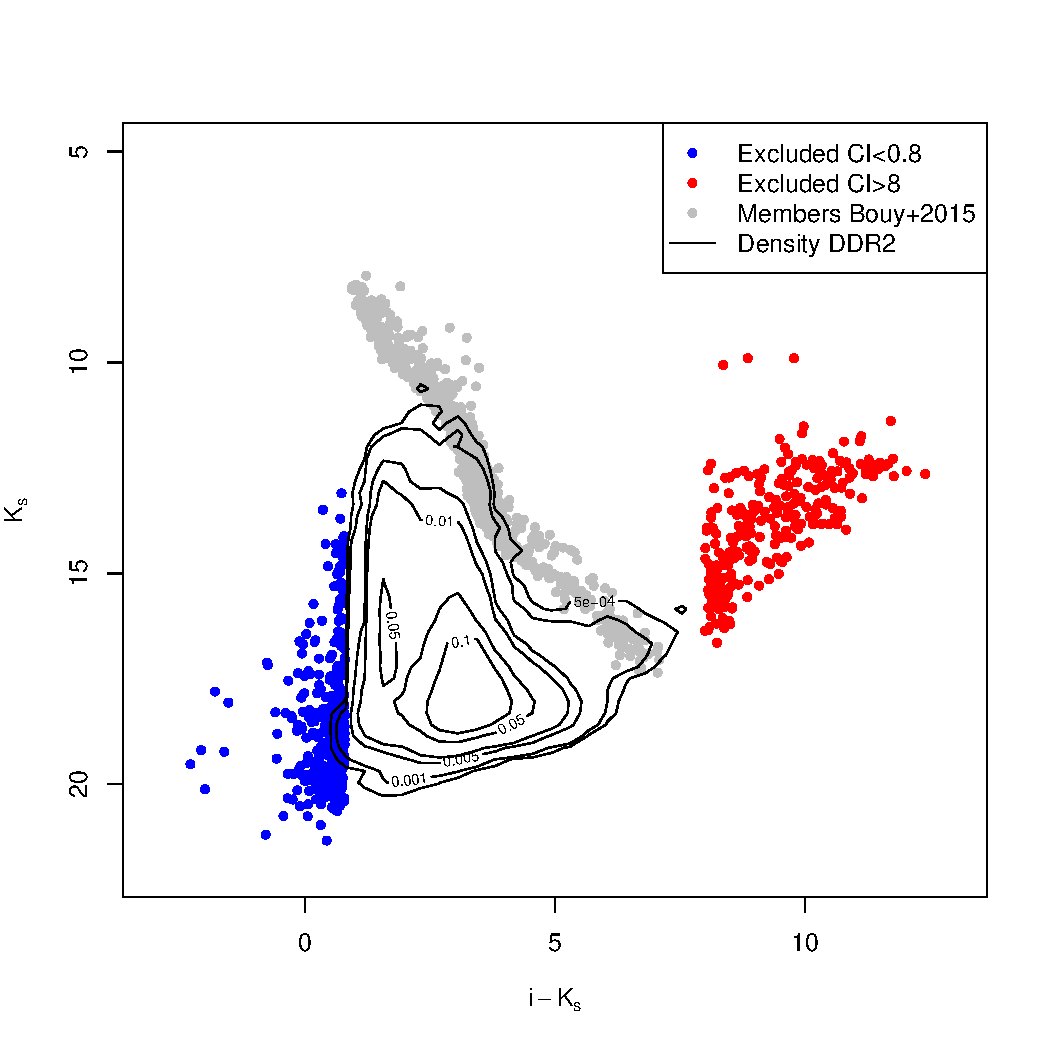
\includegraphics[width=\textwidth]{background/Figures/ColourCuts.pdf}
\caption{$K_s$ vs \gls{ci} \gls{cmd} showing the density (black contour lines) of all objects (with observed entries in this \gls{cmd}) in the \gls{ddr2}. Also shown, the candidate members of \citet{Bouy2015} (grey dots), and the objects excluded by the cuts at \gls{ci}=0.8 (blue dots) and \gls{ci}=8 (red dots). See text for details.}
\label{fig:incompatible_objects}
\end{center}
\end{figure}


With the previous restrictions to the \gls{ddr2} reduced it to 1 424 893 objects, with the largest number of rejected objects ($\sim 500\, 000$) resulting from a completely missing photometry.

\subsubsection{The Restricted DANCe Data Release 2 (RDDR2)}
Our computational constraints and the costly computations of our methodology (see Sect. \ref{sect:BHM}), prevented its application to the entire data set. However, since the precision of our methodology, as that of any statistical analysis, increases with the number of independent observations, we find that a size of $10^5$ source for our data is a reasonable compromise. Although a smaller data set produces faster results, it also renders a less precise and potentially more biased model of the field (in the area around the cluster) and therefore, a more contaminated model of the cluster. Thus, our data set was restricted to the $10^5$ objects with highest membership probabilities according to \citet{Bouy2015}. \textbf{This is equivalent to set a probability threshold at $p=1.05e^{-11}$ and select objects above this level.} In the following I refer to this data set as the \gls{rdr2}. The majority of these objects ($\sim$98\%) belong to the field with cluster membership probabilities about zero according to \citet{Sarro2014,Bouy2015}. Thus, under the assumption that the membership probabilities given by these authors are correct, the probability of leaving out a cluster member is negligible. The \gls{rdr2} data set is used to construct the cluster model and obtain the membership probability of its $10^5$ objects. For the remainder of the objects in the \gls{ddr2}, we assign membership probabilities \emph{a posteriori}, once the cluster model is constructed. 

Tables \ref{tab:rddr2_cluster} and \ref{tab:rddr2_field} show summaries of the observables and uncertainties for the 98012 field and 1988 cluster objects in the \gls{rdr2}, respectively. This classification is based on the membership probabilities and probability threshold ($p=0.75$) derived by \citet{Bouy2015}.

\begin{table}[ht!]
\caption{Summary of the 1988 candidate members of \citet{Bouy2015} in the \gls{ddr2}.}
\begin{center}
\begin{tabular}{|c|c|c|c|c|c|c|c|}
\hline
Observable & Min. & 1st. Qu. & Median & Mean & 3rd. Qu. & Max. & NA's \\
\hline
\hline
$\mu_{\alpha} [mas\cdot yr^{-1}]$&-81.64 &  14.45  & 16.24 &  16.30  & 18.14  & 90.32&0\\
$\mu_{\delta} [mas\cdot yr^{-1}]$&-81.88&  -42.09 & -39.85  & -39.62  &-37.45  & 82.59&0\\
i -$K_s$[mag] &  0.934 &   3.002 &  3.364  & 3.396 &  3.678 &  7.085  &   713\\
Y [mag]& 8.284 & 13.700 & 14.450  &14.690  &15.400 & 20.390  &   518\\
J [mag]& 6.545 & 11.950 & 13.400  &13.160 & 14.380  &19.310   &    6\\
H [mag]& 6.587 & 11.330 & 12.850  &12.610&  13.840 & 18.300   &   13\\
$K_s$ [mag]& 6.514 & 11.090 & 12.530 & 12.300 & 13.500 & 17.360   &    1\\
\hline
\multicolumn{8}{c}{Uncertainties}\\
\hline
Observable & Min. & 1st. Qu. & Median &Mean& 3rd. Qu. & Max. & NA's \\
\hline
\hline
$\mu_{\alpha} [mas\cdot yr^{-1}]$&0.08&0.25&0.76&0.5201&2.02&1e+5 &0\\ 
$\mu_{\delta} [mas\cdot yr^{-1}]$&0.08&0.25&0.76&0.52&2.02&1e+5& 0\\ 
i [mag] & 0.0200 & 0.0200 & 0.0200 & 0.0351 & 0.0202 & 2.1610&713 \\
Y [mag] & 0.0300&  0.0500&  0.0501&  0.0569&  0.0503 & 0.2392&518\\
J [mag] & 0.02000& 0.02700& 0.05005 &0.04270& 0.05014 &0.15990&6\\
H [mag] & 0.02000 &0.02700& 0.04009 &0.03994 &0.05010 & 0.14340&13\\
$K_s$[mag]&0.02000& 0.05003& 0.05045& 0.05278 &0.06001 &9.99500&1\\
\hline
\end{tabular}
\end{center}
\label{tab:rddr2_cluster}
\end{table}%

\begin{table}[ht!]
\caption{Summary of the 98012 filed objects in the \gls{rdr2}.}
\begin{center}
\begin{tabular}{|c|c|c|c|c|c|c|c|}
\hline
Observable & Min. & 1st. Qu. & Median & Mean & 3rd. Qu. & Max. & NA's \\
\hline
\hline
$\mu_{\alpha} [mas\cdot yr^{-1}]$&-99.980& -11.730  & 1.803 &  1.307 & 15.050 & 99.910&0\\
$\mu_{\delta} [mas\cdot yr^{-1}]$&-99.990& -17.980  &-4.820  &-4.088   &9.189  &99.980&0\\
i -$K_s$[mag] &   1.04 &   3.49  &  5.13    &   4.81  &  5.81  &  7.99 &  95628 \\
Y [mag]          & 9.97  & 18.70      &  19.45 &  18.83 &  19.93 &  22.23  & 21988 \\
J [mag]          & 3.954 & 17.790 & 18.660 & 17.880 & 19.160 & 20.620 &   7305\\
H [mag]         & 2.969 & 16.950 & 17.750 & 17.020 & 18.210 & 20.270  &  7655\\
$K_s$ [mag] & 2.598 & 16.260 & 16.960  &16.360  &17.370 & 21.020 &   5013\\
\hline
\multicolumn{8}{c}{Uncertainties}\\
\hline
Observable & Min. & 1st. Qu. & Median &Mean& 3rd. Qu. & Max. & NA's \\
\hline
\hline
$\mu_{\alpha} [mas\cdot yr^{-1}]$&0.08  &    8.65   &  14.94   &  23.50   &  25.60 &1.0e+05&0\\ 
$\mu_{\delta} [mas\cdot yr^{-1}]$&0.085  &   8.652  &  14.940  &  20.710  &  25.600 &1.86e+04 & 0\\ 
i [mag] & 0.02        &  0.02    &    0.07 &   0.08 &  0.12   & 0.66    &    95628 \\
Y [mag] & 0.030     &   0.068&   0.103&  0.112 &   0.148&0.938  &   21988\\
J [mag] & 0.020      &  0.065  & 0.097  & 0.104 & 0.136  &0.403   & 7305\\
H [mag] & 0.020     &  0.065  & 0.093  &0.099  & 0.124  &9.998   & 7655\\
$K_s$[mag]&0.020 &  0.060 &  0.079 & 0.087  & 0.101 & 9.998  & 5013\\
\hline
\end{tabular}
\end{center}
\label{tab:rddr2_field}
\end{table}%

\section{The Tycho+DANCe candidate members}
\label{sect:Tycho+DANCe}
Here I describe the data set used for the analysis of the Pleiades \gls{psd}. This data set is the largest and less contaminated list of Pleiades candidate members to date. It comprises, for the middle and faint luminosities, the \gls{hmps} of candidate members recovered by the \gls{bhm}, described in Section \ref{sect:memberscomparison}, and summarised in Table \ref{tab:hmps}, and for the high luminosities, the Tycho+DANCe candidate members of \cite{Bouy2015}, summarised in Table \ref{tab:tycho2}.

This joint data set comprises the positions in equatorial coordinates R.A. and Dec. (in the following $\alpha$ and $\delta$), proper motions, photometry, and membership probabilities of 2060 unique sources. 
However, for the analysis of the \gls{psd} we work only with the positions, membership probabilities, and $J$ photometric band. The latter is the bluest most available photometric band for this list of members. It will be used as a proxy for the mass, and to explore evidence of mass segregation.

\begin{table}[ht!]
\caption{Summary of the 1967 objects classified as members by the \gls{bhm}.}
\begin{center}
\begin{tabular}{|c|c|c|c|c|c|c|c|}
\hline
Observable & Min. & 1st. Qu. & Median & Mean & 3rd. Qu. & Max. & NA's \\
\hline
\hline
RA [deg]   & 51.42 &  55.67 & 56.69 &  56.76  & 57.81  & 62.81 & 0\\
Dec. [deg] &19.13  & 23.11  & 24.10 &  24.13  & 25.22 &  29.56 &0\\
$\mu_{\alpha} [mas\cdot yr^{-1}]$&-23.34  & 14.59  & 16.32 &  16.73 &  18.37  & 53.84&0\\
$\mu_{\delta} [mas\cdot yr^{-1}]$&-81.370 &-42.410& -40.130& -40.480& -37.760&  -2.016&0\\
i -$K_s$[mag] &  0.934 &  2.979  & 3.357    & 3.325   &  3.648  &6.662   &643\\
Y [mag]           &   8.284 & 13.660 & 14.360  &14.590  &15.310  &20.100 &   467 \\
J [mag]           &   7.058 & 12.060& 13.370  & 13.180 & 14.290 & 18.570&      5\\
H [mag]          &   7.009 & 11.430 & 12.810  & 12.620 & 13.750 & 17.480&      9 \\
$K_s$ [mag]  &   7.008 & 11.190 & 12.500  & 12.320 & 13.410 & 16.740&    0\\
\hline
\end{tabular}
\end{center}
\label{tab:hmps}
\end{table}%

\begin{table}[ht!]
\caption{Summary of the 207 objects from the Tycho2+DANCe data set classified as Pleiades candidate members ($P>0.48)$ by \citet{Bouy2015}.}
\begin{center}
\begin{tabular}{|c|c|c|c|c|c|c|c|}
\hline
Observable & Min. & 1st. Qu. & Median & Mean & 3rd. Qu. & Max. & NA's \\
\hline
\hline
RA [$^\circ$]                                 				            &  52.05&55.89 & 56.46 &56.55  &57.30   &  62.49  & 0\\
Dec. [$^\circ$]                       					           &  18.56&23.13  & 24.08& 23.99  &24.88  & 29.89 &0\\
$\mu_{\alpha} [\mathrm{mas}\cdot \mathrm{yr}^{-1}]$   &      9.7 &18.9   & 20.1  &    20.0 &  21.1   &  26.7&0\\
$\mu_{\delta} [\mathrm{mas}\cdot \mathrm{yr}^{-1}]]$   &  -55.10&-46.60&-45.10&-45.19 &-43.70  & -37.70&0\\
i [mag]								            &   7.910&9.321 & 10.21&  10.04 &   10.76& 12.960&   72\\
J [mag]          								    &   3.800& 7.588& 8.638& 8.451 & 9.575  &10.590&      0\\
H [mag]        								    &   3.864& 7.535& 8.463& 8.236 & 9.209  & 10.030&      0 \\
$K_s$ [mag]  							            &   3.879&7.478 & 8.373& 8.167  &  9.113 &  9.929&    0\\
\hline
\end{tabular}
\end{center}
\label{tab:tycho2}
\end{table}%

\subsection{Contamination and completeness}
\label{sect:TDContamination}
In Section \ref{sect:classifier}, we estimate a contamination rate of $4.3\pm0.2$\% in the \gls{hmps}, which
would amount to 84 of the 1967 candidate members. Also, \citet{Sarro2014} estimate that the contamination rate of their methodology is $11.0\pm2.0$\% for a probability threshold of $p=0.5$, as the one used by \citet{Bouy2015} to classify the candidate members of their Tycho+DANCe data set.  Thus, in our combined Tycho+DANCe list of candidate members, we acknowledge a mean contamination rate of $\sim 8\%$. We would expect these contaminating sources to be uniformly distributed in right ascension and declination because the position on the sky was explicitly removed from the calculation of membership probabilities.

We estimate the completeness of our list of candidate members, in terms of the J band luminosity and
spatial coverage, by assessing the completeness of the joint Tycho+DANCe survey. In Fig. \ref{fig:completeness} we show the distribution of the number of sources in the combined DANCe+Tycho catalogue as a function of the radial position for different limiting magnitudes in the J band.
The radial position is computed assuming a distance of 134.4 pc to the Pleiades cluster \citep{Galli2017} and a centre at $\alpha,\delta =[56.65,24.13]$. Distances are corrected by geometric distortions of large angles (using Eqs. \ref{eq:distfree} and \ref{eq:rs_and_ts}).
As can be seen from this figure, the DANCe+Tycho catalogue is complete until magnitude $J\sim19$ and radial distance of 11.5 pc ($\sim5^\circ$). We notice that the latter corresponds roughly with the sky coverage of the UKIDSS survey \citep{2007MNRAS.379.1599L}.
Hence, we restrict our list of candidate members to those with: i) J band observed and less than 19 mag., and ii) radial distances less than 11.5 pc. This results in 1964 candidate members, which represents more than 50\% more candidate members that those of  \citet{Converse2010}, who did the latest analysis of the Pleiades PSD.

Nevertheless, we remind the reader that the inhomogeneities (e.g. spatial resolutions, gaps in luminosity) of the data DANCe+Tycho data set are so complex (and some of them only partially understood) that can indeed bias the sample of candidate members in unknown ways. For example, the gap in luminosity coverage between the faint end of Tycho-2 catalogue and the bright end of the DANCe survey (see in Fig. 8 of \citealt{Bouy2015}) may result in undetected sources, therefore unmeasured proper motions and finally an incomplete list of candidate members.

\begin{figure}[ht!]
\begin{center}
\includegraphics[page=2,width=\columnwidth]{./background/Figures/RadiiDistribution_Tycho+DANCe_Jmag.pdf}
\caption{Density of sources in the combined DANCe+Tycho catalogue as a function of the radial distance to the cluster centre and limiting magnitude in the J band. The vertical grey line marks the limit of spatial completeness, 11.5 pc.}
\label{fig:completeness}
\end{center}
\end{figure}





%!TEX root = ../thesis.tex
\chapter{Bayesian formalism}
\label{chap:BHM}
This chapter provides a general introduction to probability theory and its application to parametric inference. The objective of this work is to infer the probability distributions of the cluster properties (e.g. luminosity and velocity). Bayes' theorem provides the proper probabilistic framework for the inference of the parameters governing these distributions. The Bayesian framework demands, though, the setting up of prior beliefs about the parameters values. Thus, later in this chapter, I  describe the reason why the Bayesian Hierarchical Models are the least subjective approach to settle down the priors. Once the posterior distribution of the parameters in the model has been analytically described, I proceed to describe the MCMC techniques and the particular one I use to sample the posterior distribution. 

In the Sections ahead I also provide the details on the assumptions I make to model the data (i.e. the likelihood), and to choose the parameters of the prior distributions. The two final sections focus on the practical issues related to the sampling of the posterior distributions, and the description of the codes I developed.

Partial results of the work presented here have been submitted to the Journal A\&A as \citet{Olivares2017}. Thus, in the following, whenever I use the pronoun \emph{we}, it refers to the authors of \citet{Olivares2017}. However, I use the pronoun I to emphasis that the particular idea or task was done by me.

\section{Introduction to probability theory.}
 
Uncertainty and probability are closely entangled. Every measurement has an associated uncertainty, otherwise is not a complete measurement \footnote{Upper and lower limits are examples of incomplete measurements.}. The term uncertainty must not be confused with the term error, which refers to the difference between the measured value of the quantity and its \emph{true} value\footnote{The true value is that which ideally results when the uncertainty tends to zero.} \citep{GUM2008}. It is commonly agreed that the uncertainty of a measurement can be expressed in a probabilistic basis \citep{GUM2008}. It means that whenever we measure a quantity, lets say $a$, the distribution of the repeated measurements of $a$, follows a probability distribution function (pdf, throughout the text I refer to it as a probability distribution or simply a distribution), $p(a)$. This $p(a)$, as any other (statistical) pdf,  satisfies the following properties:

\begin{enumerate}[label=\textbf{Property \arabic*}]
\item  It has units, those of the inverse of $a$. \label{property:1}
\item $p(a) \geq 0$. \label{property:3}
\item $1=\int_a p(a) da$. \label{property:3}
\end{enumerate}

These properties hold regardless of the dimension of $a$. It means that the joint probability distribution of the uncertainties of all measured quantities of an object is also a probability distribution. Furthermore, they also hold for conditional probability distributions. Let's imagine that we measure the positions, projected in the plane of sky (the plane perpendicular to the line of sight), of one star. The measurements are conditioned on the magnitude, or brightness, of the object we measure. If the object is too bright, like the sun, it saturates the detector and that renders the measurement useless. On the other hand, if the object is too faint, there are not enough photons to trigger a detection. So, the stellar positions in the sky, which we can call $a$ and $b$ because they are two dimensions, follow a conditioned probability distribution, with the magnitude, $c$, the conditional variable. Therefore, $p(a,b|c)$ must also satisfy:

\begin{itemize}
\item It has units of $a^{-1} b^{-1}$.
\item $p(a,b|c)\geq0$.
\item $1=\int_a \int_b p(a,b|c)da\cdot db$.
\end{itemize}

The link between joint and conditioned probabilities is given by the following symmetric definition:

\begin{align}
p(a,b)=p(a|b)\cdot p(b).\nonumber \\
p(a,b)=p(b|a) \cdot p(a),
\end{align}

which can be further conditioned on $c$ to obtain:
\begin{align}
\label{eq:conditioned}
p(a,b|c)=p(a|b,c)\cdot p(b|c),\nonumber \\
p(a,b|c)=p(b|a,c) \cdot p(a|c).
\end{align}

If the joint probability of $a$ and $b$ can be factorised, this is
\begin{align}
p(a,b)=p(a)\cdot p(b),
\end{align}
then $a$ and $b$ are say to be \emph{independent}. An alternative option is to say that $a$ and $b$ are \emph{independent} if the conditional probability of $a$ on $b$ is $p(a|b)=p(a)$.

\ref{property:3} establishes that the amount\footnote{Which could be infinite, like in Dirac's delta.} of probability distribution $p(a)$ spread over the volume of the support of $a$ adds to one. This Property allows the \emph{marginalisation} of any \emph{nuisance} variable. Let's imagine that someone gives us the probability distribution $p(a,b)$, where $a$ and $b$ are the positions of some star in the plane of the sky. If we are interested in, let's say, the mean value of $a$, we first must get rid of $b$. For it, we \emph{marginalise} it out in the following way,
\begin{align}
\label{eq:marginalisation}
p(a)=\int_b p(a,b)\cdot db.
\end{align}

Then we compute the \emph{expected value} of $a$, $E(a)$, which is identified with the mean of $a$ once we have drawn many realisations from its probability distribution. To compute it, we add all the possible values of $a$ weighted by their probability. This is,

\begin{align}
\label{eq:expectation}
E(a)=\int_a a\cdot p(a)\cdot da.
\end{align}

Once again, these last two equations (\ref{eq:marginalisation} and \ref{eq:expectation}) hold if the distributions are conditioned on any other measurement. For example, the magnitude of the object, as we did before. 

It is important to recall that the term measurement, and its unavoidable uncertainty, refer not just to directly measured quantities, like the photons (counts) and pixels in a CCD, but also to indirect measurements. Stellar magnitudes and positions in the sky, for example, are indirect measurements derived from the direct measurement of photons, pixels and telescope arrangements. This generalisation also applies to the measurement of parameters in any physical or statistical model, like the one I will describe in the following Sections.

\subsection{Bayes theorem}
The definition of conditioned probability (Eq. \ref{eq:conditioned}) leads to Bayes' theorem:
\begin{equation}
p(a|b,c) = \frac{p(b|a,c)\cdot p(a|c)}{p(b|c)}.
\end{equation}
Integrating on $a$ we find that,
\begin{align}
\label{eq:evidence}
p(b|c) \cdot \int_a p(a|b,c)\cdot da = \int_a p(b|a,c) \cdot p(a|c) \cdot da \nonumber \\
Z \equiv p(b|c) = \int_a p(b|a,c) \cdot p(a|c) \cdot da.
\end{align}
In this last equation $Z$ refers to what is known as the \emph{evidence}. This Eq. illustrates that $p(b|c)$ is a normalisation constant which can be evaluated once $p(b|a,c)$ and $p(a|c)$ are known. This turns out to be very useful, since as we will see on the following Sections, it tells us that to obtain p(a|b,c) we need just a sample of it, that can be later normalised to obtain a proper probability distribution.

\subsubsection{Models and parametric inference}
In a broad sense, models are representation or abstraction of the \emph{a priori} knowledge some one has about something. Sometimes this knowledge is also shared by others. Models are everywhere in our daily life: from the words we speak every day, to the evolution of the species and the general relativity; from a kid's drawing to cosmological models. In science, however, we restrict the concept of model to a mathematical representation of the relations (the \emph{a priori} knowledge) among the entities that the model attempts to describe. These entities include the observables (i.e. the data), and the parameters, if the model is parametric. In this later case, the observables can be reproduced by means of the parameters. Thus, a parametric model can be thought of as a function which relates parameters and observables in a mathematical way. 

The act of finding the parameters that reproduce the observables is called parametric inference. This last can focus either on the entire probability distribution of the parameters, or just on some statistics about it (e.g. the maximum a posteriori, also known as MAP, or the mean and variance).

The proper way to obtain the entire probability distribution of the parameters in a model, given the data, is through Bayes' theorem. Thus it is called Bayesian inference. Another example of parametric inference is the maximum likelihood approach. Where the likelihood, which is seen as a function of the parameters, is maximised. Despite that it properly obtains the parameters that reproduce the data, it does not return their probability distribution. Formally, the likelihood is a probability distribution on the data, and just a function on the parameters. Thus for us to obtain the probability of the parameters we must multiply this likelihood times the priors and normalise it. THis is what Bayes' theorem does.

In this context, Bayes' theorem is:
\begin{equation}
p(\mathbf{\theta}|\mathbf{D},\mathcal{M}) = \frac{p(\mathbf{D}|\mathbf{\theta},\mathcal{M})\cdot p(\mathbf{\theta}|\mathcal{M})}{p(\mathbf{D}|\mathcal{M})}.
\end{equation}
where $\mathbf{\theta},\mathbf{D}$ and $\mathcal{M}$ correspond, respectively, to the parameters in the model, the data which the model tries 
to describe, and the the model itself. 

The term on the left is called the posterior probability distribution of the parameters, $\mathbf{\theta}$ given the data $\mathbf{D}$ and the model $\mathcal{M}$. In the right side, the two terms in the numerator are called \emph{likelihood}, $p(\mathbf{D}|\mathbf{\theta},\mathcal{M})$ and \emph{prior}, $p(\mathbf{\theta}|\mathcal{M})$. As mentioned earlier, the denominator, $p(\mathbf{D}|\mathcal{M})$, is called the \emph{evidence}. 

Formally, the likelihood and the prior are probability distributions on the data $\mathbf{D}$ and the parameters $\mathbf{\theta}$, respectively. However, for the posterior to be a probability distribution on the parameters, it only suffices that the product of the likelihood times the prior does not vanish everywhere or be negative anywhere\footnote{See Property 2. Although negative probabilities may have sense in quantum mechanics. See for example \citet{1942RSPSA.180....1D}}. If these are not probability distributions, they are called \emph{improper} priors or \emph{improper} likelihoods. In the extreme case that their product vanishes everywhere, which may be the case if the prior is terribly specified or if the likelihood does not take proper account of extreme data, the posterior will not be a probability distribution due to a division by zero. Nevertheless, it makes no sense to try to estimate the parameters of a model with zero evidence.

%Whenever we have a model $M$, we have also the \emph{a priori} knowledge used to construct it. Actually, it can be classified in two kinds of prior information. One refers to the prior information conveyed in the model, which I call $M$. This is the information that the creator of the model uses to establish the relations among the elements of the model: variables. The second kind of prior, $p(\mathbf{\theta}|M)$ refers to the statement the user of the model made of his/her beliefs about the probability distribution of the parameter values. This is indeed subjective. However, it is, in my opinion, less subjective than the former, $M$, prior information. At least in this last kind, the subjectivity is expressed objectively in a probabilistic, and therefore measurable way.
%
%The likelihood of the data $p(\mathbf{D}|\mathbf{\theta},M)$, is a probability distribution on the data, $\mathbf{D}$. However, it is a function on the parameters, $\mathbf{\theta}$, which corresponds to the function $f$ of Eq. \ref{eq:model}. This function is not necessarily a probability distribution on the parameters. 

As mentioned before, the likelihood is the probability distribution of the data given the parameters, regardless the size of the data set. Almost always the data set is a collection of measurements of several objects, but it could also be made of just one object. Thus, to obtain the likelihood of the data based on that of the individual objects, some assumption must be made. 

When measuring the properties of individual objects in a collection of them, almost always it is assumed that measurements, and therefore their probability distributions, are independent within objects of the collection. For example, if we were to measure the weight of a group of persons, we usually assume that the pdf of the weight of one person, is independent of that of another person. This assumption, however, does not always holds. Imagine for example, that we were conducting a statistical analysis on the length of the objects used to define our unit of length. In this case, the statistical distribution of the length of any object depends on the unit of measurement, which in turn is depends on the distribution of measured lengths of the rest of the objects. Therefore, the individual probability distributions of the length of the objects are not independent within them\footnote{This happens for example in satellite surveys for which their system of reference is defined by their own measurements. To avoid this issue their reference systems are anchored on independent measurements.}. 

If we assume that the probability distribution of the measured value, $d$, of a collection of $N$ objects are independent within them, then
\begin{equation}
\label{eq:independence}
 p(\mathbf{D}) = \prod_{n=1}^N p_n(d_n), \ \ n=\{1,2,...,N\}
\end{equation}

 with $p_n$ explicitly stating that the individual probability distributions are distinct. 
 
 Thus, the likelihood of the data, $p(\mathbf{D}|\mathbf{\theta},M)$ can be expressed as,

\begin{equation}
\label{eq:lik_datum}
 p(\mathbf{D}|\mathbf{\theta},M) = \prod_{n=1}^N p_n(d_n|\mathbf{\theta},M), \ \ n=\{1,2,...,N\}.
\end{equation}

The term $p_n(d_n|\mathbf{\theta},M)$ is the likelihood of datum $d_n$. This is also called the \emph{generative} model, since it  contains the necessary information to generate the data\footnote{It may also contain the uncertainty process that transform the \emph{true} data into the noisy observations.}.

To summarise, Bayes' theorem can be interpreted as the probabilistic way to update knowledge. To me, it embodies the process of knowledge improvement once we recognise that knowledge is uncertain, which in my perspective, is always uncertain. Even when its uncertainty is negligible under the current evidence that supports it. Bayes' theorem helps us to update our prior knowledge once we multiply it by the likelihood of the data. Then, the posterior probabilities, became our new knowledge. 

Furthermore, the Bayes' theorem also provides the objective way to compare two models or hypothesis, and update the a priori knowledge used to construct them. This is called model selection, which I  briefly explain in the next section.

\subsection{Model Selection}
\label{sect:modelselection}

Whenever we have a data set and two or more models that attempt to describe this data, the most straightforward thing to do is to compare these models. Almost always, we want to select the \emph{best} model. Obviously the term \emph{best} depends on the objective of research. For example, let's imagine that our data set consists of the positions of an object as function of time. If we were interested in reproducing exactly the same points in the data set, the \emph{best} model will be a polynomial with degree equal to the number of points. This polynomial will pass trough all these points. However, once we recognise the unavoidable uncertainty of the data, we realise that an exact representation of the data may be of no use since it fits also the noise of the data. 

In general, we are interested in the predictive capabilities of a model, its ability to predict future observations rather than to replicate the ones we currently have. Thus, an exact representation of the observed data (an over-fitted model as in the previous example), will poorly describe any new data set. In this sense, an over-fitted model \emph{memorises} the data rather than \emph{learns} from it.

A model that \emph{learns} from the data is that which recovers the \emph{true} underlying relation embedded in the data. This \emph{true} underlying relation is the one that produces the \emph{true} data. The observed data results once the uncertainty process is added. 

Nevertheless, we still need to select among different learning models.  

We can draw some help from the commonly known Ockham's razor or principle \footnote{The origin of this motto and its exact phrasing is beyond the scope of this work. I just mention that paradoxically, an ancient formulation is attributed to Ptolomey: "We consider it a good principle to explain the phenomena by the simplest hypothesis possible" \citep{Franklin2002}}. It says:
\begin{quotation}
\textit{Among competing hypotheses, the one with the fewest assumptions should be selected.}
\end{quotation}

Here, hypotheses can be identified with models. Thus, this principle tells us we should choose the model that makes the fewest assumptions. I classify the assumptions of a model in two groups: fixed and free ones. The fixed assumptions belong to what I previously described as the \emph{a priori} knowledge used to construct the model. These may render the model more interpretable in the physical or statistical sense, or even give it coherence within the corpus of a theory. The free assumptions on the other hand, correspond directly to the parameters in the model. They give it flexibility when fitting the data\footnote{However, they can also introduce degeneracy in the parametric space.}. For example, in the case of a straight line model, the fact that the data is linearly related can be considered as a fixed assumption. The free assumptions correspond to the slope and ordinate at the origin. 

When comparing a linear model to a quadratic one in which the constant term has been fixed, we see that they have the same number of free parameters, two, but clearly the second one has an extra fixed assumption. Therefore, choosing the model with fewer free parameters does not necessarily means choosing the model with the fewest assumptions.

One of the great advantages of the Bayesian methodology is that it incorporates directly Ockham's principle. Suppose that we want to compare two models, $M_1$ and $M_2$, which we assume describe the data set, $\mathbf{D}$. Each model has prior probabilities, $p(M_k)$ and likelihoods $p(\mathbf{D}|M_k)$ (with $k=1,2$). Notice that now, I use Bayes' theorem for models and not for parameters within a model. So, the prior probabilities of the models reflect our beliefs about the fixed assumptions within each model. On the other hand, the likelihood of the data given the model, is related to the parameters (the free assumptions) and their prior probabilities, both within a model. This likelihood of the data given the model corresponds to the \emph{evidence} of the model (Eq. \ref{eq:evidence}). This evidence in terms of the model parameters, $\theta_k$, is now

 \begin{equation}
p(\mathbf{D}|M_k)=\int_{\theta_k} p(\mathbf{D}|\theta_k,M_K)\cdot p(\theta_k|M_k)\cdot d\theta_k. \label{eq:evidence2}
\end{equation}
Bayes' theorem applied to models, instead of individual parameters as done before, tells us that
\begin{equation}
p(M_k|\mathbf{D})=\frac{p(\mathbf{D}|M_k)\cdot p(M_k)}{p(\mathbf{D})},
\end{equation}
with $k=1,2$. Since there are only two models, their prior probabilities are related by $p(M_1)= 1- p(M_2)$. Therefore,
 \begin{equation}
p(M_k|\mathbf{D})=\frac{p(\mathbf{D}|M_k)\cdot p(M_k)}{p(\mathbf{D}|M_1)\cdot p(M_1)+p(\mathbf{D}|M_2)\cdot p(M_2)}.
\end{equation}
From this last Equation, the ratio of the posterior distributions is:
\begin{equation}
\frac{p(M_1|\mathbf{D})}{p(M_2|\mathbf{D})}=\frac{p(\mathbf{D}|M_1)\cdot p(M_1)}{p(\mathbf{D}|M_2)\cdot p(M_2)}.
\end{equation}
This ratio provides an objective measure of how better the model $M_1$ is when compared to model $M_2$, under the measure provided by the data $\mathbf{D}$ by means of the evidence. When both prior probabilities  $p(M_1)$ and $p(M_2)$ are set alike, the ratio of posteriors equals the ratio of likelihoods. This is known as the \emph{Bayes factor} \cite[for a similar derivation and some examples of its application see][]{Kaas1995}. 

Even when the priors for the models are set alike, the evidences themselves (Eq. \ref{eq:evidence2}) embody Ockham's principle. The evidence is the integral, in parametric space, of the prior times the likelihood, with the likelihood acting as a weight to the priors.  Then, the larger the number of parameters (free assumptions) is, the greater the volume over which the integral must be carried on, and the most spread the prior probability gets. Thus, unless the likelihood increases as well, the evidence is smaller in models with larger number of parameters.

As explained in this section, the paramount importance of Bayes' theorem comes from the fact that it is the proper probabilistic way to update knowledge based on evidence.

\subsection{Membership probability}

In the previous Section we obtained the probability of two competing models $M_1$ and $M_2$ given the data $\mathbf{D}$. In this Section, I describe a similar problem: the probability of two competing models given the likelihood of a single datum, $\mathbf{d}$. It also can be interpreted as the probability that the datum $\mathbf{d}$ was generated by model $M_k$. This probability is commonly known as the membership probability of the datum $\mathbf{d}$ to belong to model or class, $M_k$ ($k=1,2$). 

Bayes' theorem for this particular case is,

\begin{equation}
\label{eq:prob}
p( M_k | \mathbf{d}) =\frac{p(\mathbf{d}|M_k)\cdot p(M_k)}{\sum_{k=1}^2 p(\mathbf{d}|M_k)\cdot p(M_k)},
\end{equation}

where $p(\mathbf{d}|M_k)$ is the likelihood of datum $\mathbf{d}$ and, $p(M_k)$ is the prior probability of model $M_k$.
\section{Bayesian hierarchical Models}
\label{sect:BHM}
\subsection{Generalities}
Th Bayesian formalism requires the establishment of priors. As mentioned before, priors represent the \emph{a priori} belifes the user of the model has about the possible values that parameters of the model can take. This is indeed subjective. This subjectivity is the main source of criticism from the non-bayesian community \footnote{See \citet{Gelman2012} for a discussion on the ethical use of prior information}. 

Bayesian hierarchical models, in the following (BHM), are classified within the Empirical Bayes methods. On these methods, the prior distributions are inferred from the data rather than being directly specified, as it is done in common Bayesian methods. Particularly, in BHM the priors are specified by parametric distributions whose parameters are also drawn from a parametric distribution in a hierarchical fashion. For this reason, hierarchical models are also called multilevel models. A fully-BHM is that in which the parameters at the higher hierarchy are drawn from a non-parametric distribution. In a non fully-BHM the settlement of parameters stops at some level. These end-level parameters are called hyper-parameters.

Given their properties, the BHM represent the most objective way to the establishment of prior distributions \citep{Gelman2006}. Regardless of the level of the BHM, for it to be effective, the family, or class, of prior distributions must be carefully chosen. These families must allow the \emph{true} value of the parameter of interest \citep{Morris1983}. If the likelihood is not fully allowed by the prior (for example when the likelihood, as a function of the parameters, has a maximum outside the domain of a truncated prior.), then the inferred posterior could be biased. For this reason, inspecting and updating the prior knowledge is an important step in any Bayesian study.

Despite their theoretical advantages, BHM are difficult to evaluate since they require far more parameters than standard Bayesian methods.
Furthermore, their hierarchy (levels) must stop at some point. There are at least two approaches to stop this hierarchy. The first one is to use a non parametric distribution for the parameters at the higher level. This renders, as previously said, a fully-BHM. However, it has the inconvenience that to use a non-parametric distribution we must have certain a priori knowledge about it, which, most of the time is not the case. Another more practical alternative is to give a point estimate, usually the mean or the mode, for the distribution of the parameter at the top of the hierarchy.  

Although in BHM the parameters values of the prior distributions are inferred from data, the user of the model has the important task of specifying the family of distributions to be used for the priors. Selecting these families continues to be an active area of research. Common options include conjugate, objective, non-informative, and weakly informative priors. 

Conjugate priors are those in which the posterior distribution turns out to be in the same family as the prior one, they are called the conjugate of the likelihood. Objective or default priors are supposed to be the default choice in the absence of any other information. 
Weakly and non-informative informative priors, as their names indicate, provide intentionally weaker information or no information at all for the prior. 

Objective and non-informative priors are discarded since for the Pleiades (one of the most studied cluster in the literature) there is already sensible information that  should be used. Conjugate priors do not necessarily agree with the previous information. Thus, whenever possible, I choose the weakly informative priors. These are the option recommended by \citet{Gelman2006,Gelman2008,Huang2013} and \citet{Chung2015}, since they show better computational performance when compared to non-informative priors. Despite the family of prior distribution that we choose, we must always analyse the prior distribution in terms of the posterior, and check if this last make sense \cite[][ Chap. 6]{Gelman2006,Gelman2013}.


\subsection{Examples}
Since BHM usually need more parameters than standard techniques, its use was restricted until modern and faster computers were widely available. The concept of BHM was already present in the 1960s, however, it was not until  the 1970s that they were used to infer parameters of normal distributions and linear models \cite[see][for an historical perspective of BHM]{Good1980}. In modern days, BHM have a wide range of applications. Just to cite some examples, \citet{Gelman2007} use them in the social sciences, \citet{Fei2005} applies them for vision recognition and, \citet{Diard2008} for robot navigation.

The BHM are also widely applied in astrophysics. Although, originally its use was mainly in the domain of inference of cosmological parameters \cite[see for example the works of][]{Feeney2013,March2014,Anderes2015,Shariff2016,Alsing2017}, they were rapidly adopted in other domains. For example, they have been used to study the eccentricity distribution of binary stars \citet{Hogg2010}, the Cepheids \citep{Barnes2004} and RR Lyrae distances \citep{Jefferys2007}, the chemical composition \citep{Wolfgang2015} and albedos of exoplanets \citep{Demory2014}, extinction maps \citep{Sale2012}, stellar parameters \citep{Shkedy2007}, and the present day mass distribution \citep{Tapiador2017}.

\subsection{Graphical representation.}
\label{sect:PGM}
In general, BHM have large number of parameters that, together with the relations among them tend to obscure its understanding. To aid in this understanding, a graphical representation is always useful. Probabilistically Graphical Models (PGM) provide the background to graphically depict the BHM. PGM are graphs that portray the conditional relation among the elements in a probabilistic model. These elements could be constants or stochastic variables that interact by means of conditional relations, which could be deterministic or stochastic. 

In PGM, stochastic variables are represented with circles while constants with squares. If the variable is known, as in the case of the data, it is represented with a filled symbol, otherwise with an empty symbol. Stochastic and deterministic relations are depicted with solid and dashed lines, respectively. If there is no line between two given elements, it indicates that they are assumed to be independent. Variables that repeat together, as in the case of the data, are grouped within a plate. The number of repetitions is indicated in one corner of the plate. For more details on PGM see for example the book of \citet{Koller2009}. 

To exemplify the use of PGM, Figure \ref{fig:pgmGMM} shows the PGM for the BHM that infer of the parameters in a Gaussian Mixture Model. In this model the parameters are the means $\mu_k$, variances $\sigma_k^2$ and fractions $\phi$ of each of the $K$ gaussian distributions in the mixture. Then $\mu_0,\sigma_0^2,\lambda,\nu$ and $\beta$ are the hyper-parameters, while $x_i$ represent the data, and $z_i$ the categorical latent variable that indicates the parent gaussian for datum $x_i$.

\begin{figure}[ht!]
\begin{center}
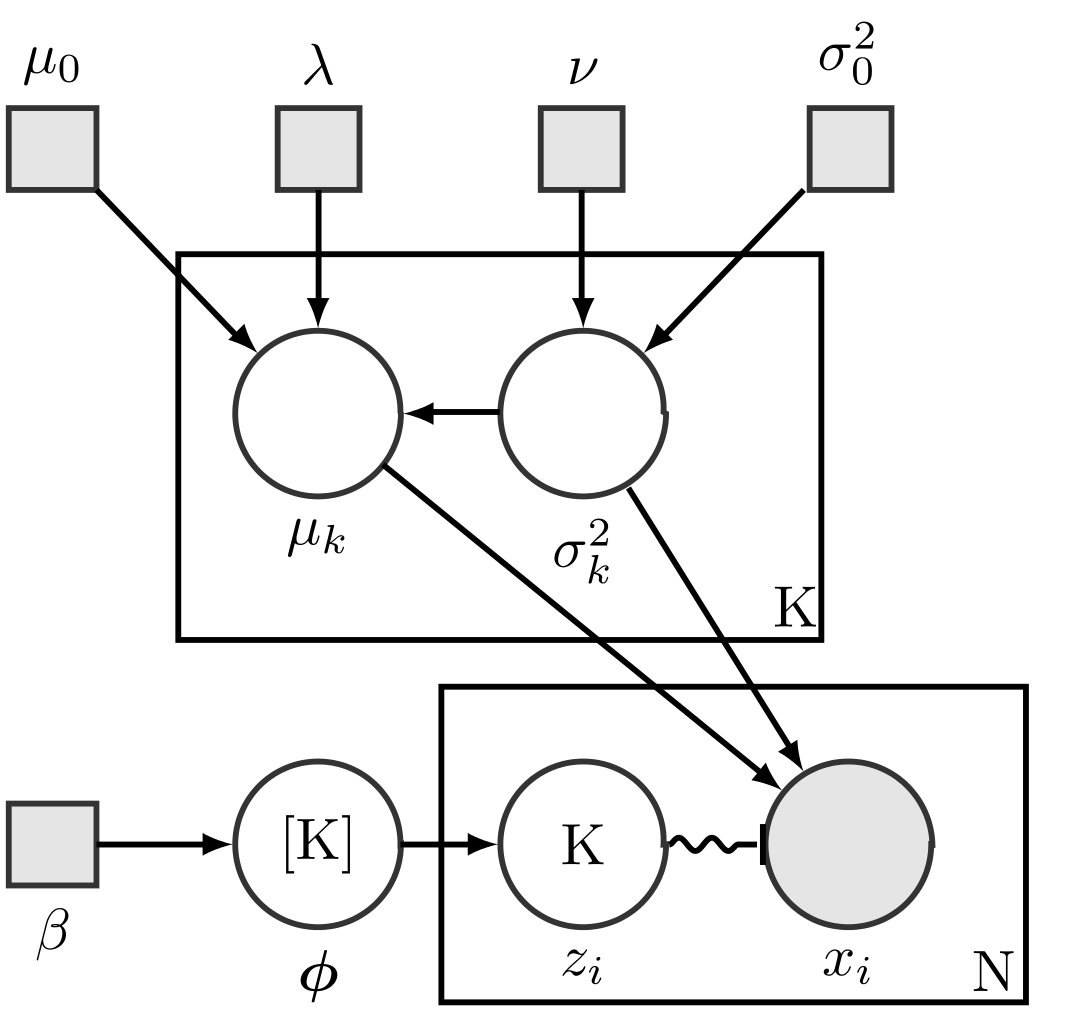
\includegraphics[height=8cm]{background/Figures/BGMM.png}
\caption{PGM representing the parametric inference of a Gaussian Mixture, see text for details. Figure by Benwing /CC BY}
\label{fig:pgmGMM}
\end{center}
\end{figure}

\section{Modelling the data}
\label{sect:datamodelling}
Creating a model is a complex task. As previously mentioned, a model is the mathematical representation of the knowledge about certain phenomenon. In this work my objective is the statistical modelling of the DANCe data related to Nearby Young Open Clusters ( NYOC), particularly the one of the Pleiades (see Section \ref{sect:DR2}).

Modelling a data set demands the gathering and arranging of the \emph{a priori} knowledge on the phenomenon. This knowledge comprises that of the data set , the NYOC: the Pleiades open cluster (Chapter \ref{chap:pleiades}), the statistical techniques that may help to attain the objective, and the computational resources at hand. I collect this knowledge from three main sources: the standard references (e.g. articles and books), my colleagues and experts on the field (\emph{knowledge elicitation}), and my self.

The structuring of the a priori knowledge and later creation the model is an iterative and continuous process.  In this Section, I describe a snapshot of this process: the state of the model once the article \citet{Olivares2017} was submitted. Later in Section \ref{sect:code}, I will give a brief description of the chronological development of the model.

In this section I will explain the statistical procedure to deal with one of the crucial aspects of the Pleiades DANCe DR2 data set: the missing values. Also, I will describe how the relevant knowledge about Pleiades cluster population and the empirical one of the field are embedded in the generative model of the data.

\subsection{Missing values}
\label{sect:missing}

Missing values refer to a non-measured or non-available (NA) value in the vector of measurements of an object. They can arise due to different statistical or physical processes. 

From the physical perspective, they occur due to faint or bright sources that produce counts values outside the dynamical range of the detector. They can also emerge due to detector malfunctions, e.g. electronic failures, or to random effects, e.g. cosmic rays. 

From the statistical perspective, important aspects of missing values are, i) the probability distribution of the sources in which they occur, and ii) if they originate due to censoring or truncation. 

In the DANCe DR2, missing values occur only in the photometric measurements (see Table \ref{tab:DR2properties}), with the bluer bands being the most affected. As expected, the probability distribution of sources with missing values is not random (uniform). Missing values occur with higher probability at the faintest and brightest ends of the photometric distributions, see Figure \ref{fig:NAsKs}. This is a crucial aspect for the statistical analysis. If missing values were randomly distributed, then, any statistical analysis derived using only objects with completely observed vectors will be unbiased. This will occur because the objects with completely observed vectors will be a random sample of the data set. Since this is not the case in the DANCe DR2, to avoid biases, objects with missing values must be incorporated in the data set and properly treated. 

\begin{figure}[ht!]
    \centering
    \begin{subfigure}[t]{0.45\textwidth}
        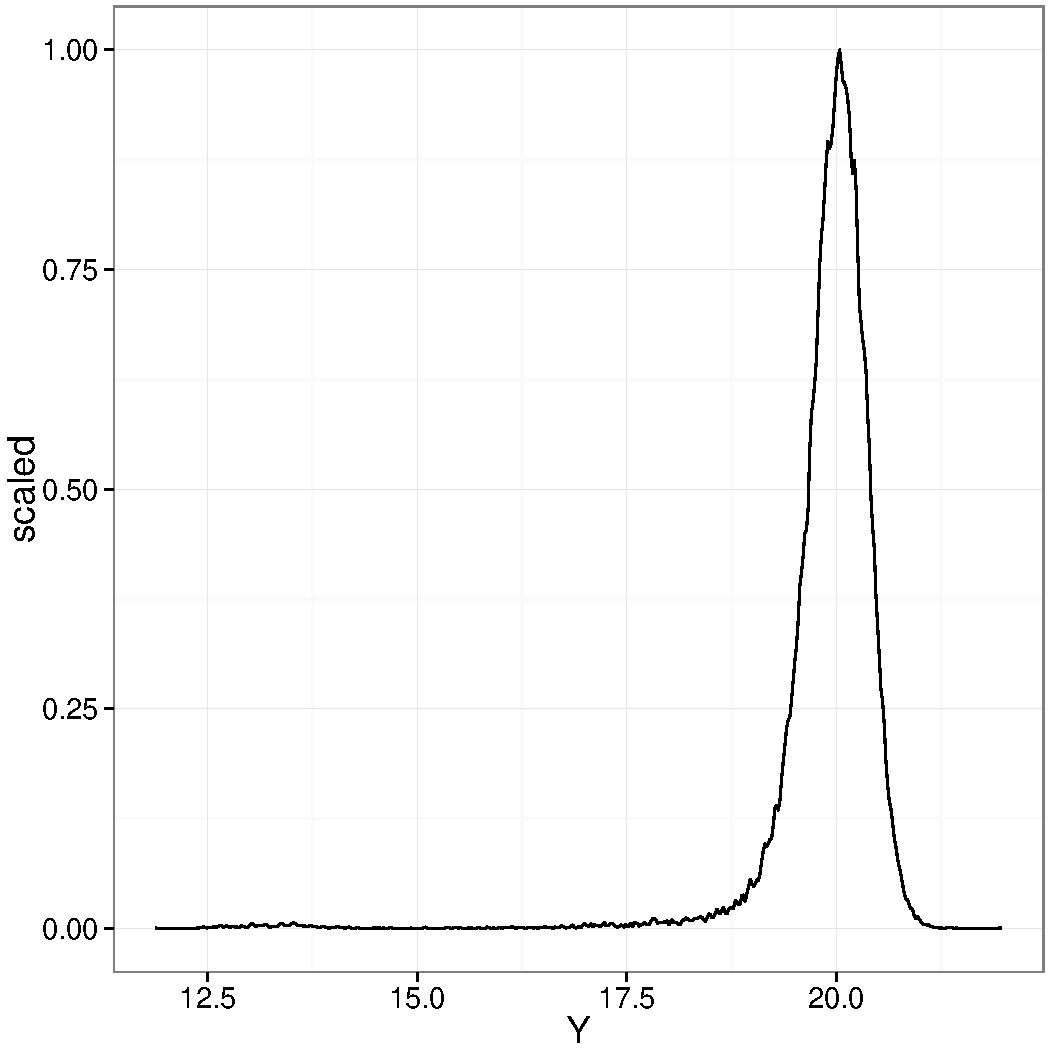
\includegraphics[page=1,height=6cm]{background/Figures/MissingDistribution.pdf}
        \caption{}
        \label{}
    \end{subfigure}
    \begin{subfigure}[t]{0.45\textwidth}
      \includegraphics[page=2,height=6cm]{background/Figures/MissingDistribution.pdf}
        \caption{}
        \label{} 
    \end{subfigure}
     \begin{subfigure}[t]{0.45\textwidth}
      \includegraphics[page=3,height=6cm]{background/Figures/MissingDistribution.pdf}
        \caption{}
        \label{} 
    \end{subfigure}
     \begin{subfigure}[t]{0.45\textwidth}
      \includegraphics[page=4,height=6cm]{background/Figures/MissingDistribution.pdf}
        \caption{}
        \label{} 
    \end{subfigure}
\caption{Probability distributions of objects with missing values. The vast majority of objects with missing values are located at the faint end of the magnitude distributions.}
\label{fig:NAsKs}
\end{figure}




Truncation occurs when the data set does not contain record, nor of the measured value neither of the number of measurements, when the measured quantity lies outside certain limits. On the other hand,  censoring happens when the data set contains only partial information about the actual value of the measured quantity. Basically,  censoring happens when the value lies outside the upper or lower limits of the measuring instrument, and these limits become the only available record of the measurement. Currently, the DANCe DR2 does not provide upper or lower limits for the censored data. Although these limits could also be inferred from the data, the  heterogeneous origin of the DANCE DR2 prohibits this task. Furthermore, the missing values in the DANCE DR2 data set do not occur only because of censoring. Indeed, cosmic rays, hot pixels, halos of bright stars, diffraction patterns and cross-matching failures are just some examples of potential sources of missing values. The statistical treatment of missing values originating from all these sources lies beyond the scope of this work. However, there is a general way to deal with missing values despite their origin.

In terms of probability, there is no distinction between missing values and parameters. Therefore, we can marginalise missing values as we do with any other nuisance parameter. If the vector of measurements $\mathbf{d}$ has a missing value in entry $i$, then $x_{i} = NA$ , and $\mathbf{d}=\{x_1,x_2,...,NA,...,x_n\}$, with $n$ the dimension of $\mathbf{d}$. Thus, the marginalised likelihood of this datum, given model parameters $\mathbf{\theta}$ is

\begin{equation}
\label{eq:marginalmiss}
p(\mathbf{d}|\mathbf{\theta})= \int_{-\infty}^{\infty} p(\{x_1,x_2,...,x_{i}= NA,...,d_n\}|\mathbf{\theta})\cdot dx_{i}.
\end{equation}

Throughout this work, missing values are marginalised in this way.

%I made a remark of a point that may seem obvious but it is important to remember. Let $p(a)$ be a probability distribution, $A$ a random sample of $n$ points from it, and $p_A(a)$ the empirical probability distribution of $A$. Let $B$ be a non-random sample of $p(a)$ with $n$ elements, and empirical probability distribution $p_B(a)$. In the limit of $n\rightarrow \infty$, $p_A(a)=p(a)$ however $p_B(a)\neq p(a)$. Therefore, $p_A(a)\neq p_B(a)$. Similarly, in data with missing values, if the missing value pattern is not random, the distribution of the completely observed data (with non-missing values) differs from that of all the data. In \citet{Olivares2017} we show this subtle but important difference in the case of the DANCe data set. 

\subsection{The generative model}
\label{subsect:generative-model}
The objective of this work is the statistical study of NYOC, in particular the Pleiades cluster. Since the Pleiades data is mixed with that of the field, to achieve the objective, cluster and field populations must be disentangled. The probabilistic disentanglement of them, demands probabilistic models for each population. These models correspond to the are the field and cluster likelihoods. With these and the prior distributions, I am able to reach the objective: the posterior distributions of the parameters in the cluster model. 

In addition, cluster membership probability distributions (Eq. \ref{eq:prob}) can be computed for each object in the data set. Using these membership probability distributions together with a probability threshold, individual objects are separated into cluster and field populations.

The inference process demands a set of $N$ binary integers $\mathbf{q}$, one $q_n$ for each object. The two possible values of these binary integers represent one of the two mutually exclusive possibilities: the object belongs to the cluster ($q_n=1$) or to the field population ($q_n=0$). 

Let $\theta$ and $\phi$ be the parameters of the cluster and field models, and $p_c$ and $p_f$ their likelihoods, respectively. Then, the likelihood of the data is,

\begin{equation}
p(\mathbf{D}|\mathbf{q},\theta,\phi)= \prod_{n=1}^N {p_c(\mathbf{d}_n|\theta)}^{q_n}\cdot {p_f(\mathbf{d}_n|\phi)}^{(1-q_n)}.
\end{equation}

The inference of these $N$ binary integers will demand a computing power that is outside the current possibilities. Thus, instead of inferring them I marginalise them. 

I marginalise these $\mathbf{q}$ using a prior probability, which is set in terms of a new and unique parameter $\pi$. It represent the \emph{prior} probability that an object belongs to the field. Thus, the prior probability of $\mathbf{q}$ is

\begin{equation}
p(\mathbf{q}|\pi)= \prod_{n=1}^N {(1-\pi)}^{q_n}\cdot {\pi}^{(1-q_n)}.
\end{equation}

The marginalisation runs as

\begin{align}
p(\mathbf{D}|\pi,\theta,\phi)&=\int_{\mathbf{q}} p(\mathbf{D},\mathbf{q}|\pi,\theta,\phi)\cdot d\mathbf{q} \nonumber \\
&=\int_{\mathbf{q}} p(\mathbf{D}|\mathbf{q},\pi,\theta,\phi)\cdot p(\mathbf{q}|\pi)\cdot d\mathbf{q} \nonumber \\
&=\int_{\mathbf{q}} \prod_{n=1}^N {p_c(\mathbf{d}_n|\theta)}^{q_n}\cdot {p_f(\mathbf{d}_n|\phi)}^{(1-q_n)}\cdot \prod_{n=1}^N {(1-\pi)}^{q_n}\cdot {\pi}^{(1-q_n)}\cdot d\mathbf{q} \nonumber \\
&=\int_{\mathbf{q}} \prod_{n=1}^N \left[(1-\pi)\cdot p_c(\mathbf{d}_n|\theta)\right]^{q_n}\cdot \left[\pi\cdot p_f(\mathbf{d}_n|\phi)\right]^{(1-q_n)}\cdot d\mathbf{q} \nonumber \\
&=\prod_{n=1}^N (1-\pi)\cdot p_c(\mathbf{d}_n|\theta) + \pi\cdot p_f(\mathbf{d}_n|\phi).
\end{align}
This last equality is a rather complicated derivation which can be found on \citet{Press1997} and in \citet{Hogg2010a} for $p_c$ and $p_f$ in the exponential family. Also, a general derivation of this expression is given by \citet{Jaynes2003}. He obtains it assuming individual unknown probabilities $p_n$ instead of $q_n$ and marginalising over them by the aid of a prior.

Thus, the \emph{generative model} or likelihood of the datum $\mathbf{d_n}$  is

\begin{equation}
\label{eq:genmod}
p(\mathbf{d}_n | \pi,\boldsymbol{\theta}_c,\boldsymbol{\theta}_f,\mathbf{u}_n)=\pi \cdot p_f(\mathbf{d}_n|\boldsymbol{\theta}_f,\mathbf{u}_n) + (1-\pi)\cdot p_c(\mathbf{d}_n| \boldsymbol{\theta}_c,\mathbf{u}_n),
\end{equation}

where $\boldsymbol{\theta}_f$ and $\boldsymbol{\theta}_c$ indicate the cluster and field parameters, while $\mathbf{u}_n$ refers to the datum uncertainty. The probabilities $p_f(\mathbf{d}_n|\boldsymbol{\theta}_f,\mathbf{u}_n)$ and $p_c(\mathbf{d}_n| \boldsymbol{\theta}_c,\mathbf{u}_n)$ are the field and cluster models, respectively. These models are explained in detail in the next two sections.

In the following, I assume that the observed quantities, even if they contain missing values, resulted from the convolution\footnote{The addition of two stochastic variables is analogous to the convolution of their probability distributions.} of the \emph{true} quantities with a source of uncertainty. This last could be different for each object, thus resulting in different individual uncertainties. It means that the DANCE DR2 data is modelled allowing for its intrinsic heteroscedaticity. Although these uncertainties are not assumed to have the same values, I do assume that they have the same shape. Thus, I assume that uncertainties in our data set belong to the multivariate normal family.  This assumption is standard practice and is also supported by the large and heterogeneous origins of the DANCe DR2 data set. 

\subsection{The field population}
To model the field population, I assume that the joint seven-dimension probability distribution of the field can be factorised into the probability distributions of proper motion and photometry. Thus, the field likelihood of the proper motion and the photometry are assumed to be independent, at least conditioned on their parameters. Also, I assume that both distributions are described by Gaussian Mixture Models (GMM). The flexibility of GMM to fit a variety of distribution geometries make them a suitable model to describe the field density of the heterogeneous DANCe DR2 data. 

A GMM is a probability distribution resulting from the linear combination of $M$ gaussian distributions, $\pi_m\cdot \mathcal{N}(\boldsymbol{\mu}_m,\boldsymbol{\Sigma}_m)$, with $m=1,2,...,M$. Where $\pi_m$ is the amplitude or fraction of the $m$th gaussian. These $m$ fractions must add to one. Thus, the probability distribution resulting from a GMM is

\begin{equation}
p_{GMM}(x|\boldsymbol{\pi},\boldsymbol{\mu},\boldsymbol{\Sigma})=\sum_{m=1}^M \pi_m \cdot \mathcal{N}(\boldsymbol{\mu}_m,\boldsymbol{\Sigma}_m).
\end{equation}

Notice that the number of gaussians in the mixture is not formally speaking a parameter, but rather it implies a collection of parameters. The number of these parameters increases quadratically with the number of gaussians. 

According to \citet{Bouy2015}, the number of Pleiades candidate members in the DANCe DR2 data set is 2010 (going up to 2109 in the combined Tycho-DANCe DR2). It means that the number of field objects dominates (99.9\%) the DR2 data set. Even in our restricted $10^5$ data set, RDR2 (see Sect. \ref{sect:RDR2}), the field still dominates with a 0.98 fraction. Thus, it can be assumed that any new classification of candidate members will have a negligible impact on this figure. Therefore, it seems reasonable to assume that the GMM describing the field population can be frozen (fixed) during the process of cluster parameters inference. Let me elaborate on this assumption.

The objects that \citet{Bouy2015} classified as field are those whose cluster membership probabilities are lower than 0.75. This probability threshold corresponds to the one found by \citet{Sarro2014} after analysing the performance of their methodology when applied to synthetic data sets. In \citet{Sarro2014} the authors report that, at probability threshold $p=0.75$, the contamination and true positive rates are $\approx 8\%$ and $ \approx96\%$ respectively. Assuming that these values are correct, the number of hypothetically misclassified objects is $12\%$ of the cluster members, thus $\approx 241 $ objects. This value is negligible compared to the size of the data set ($10^5$ objects in the RDR2). It represents the negligible fraction of $ \lesssim0.0024$. 

It can be further assumed that these hypothetically misclassified objects are spread in the observables space. Indeed, these misclassified can be thought to have membership probabilities near the classification threshold. Thus, they lay in the entanglement region which corresponds, in proper motions, to a halo around the cluster centre, and in photometry, to a region around the cluster sequence.

%Furthermore, under the assumption that the work of \citet{Sarro2014} is correct, the misclassified objects concentrate on cluster membership probabilities near the classification threshold. Therefore, they will also group in an area of the physical "boundary" between the cluster and the field (I call it physical because it is on the observable variables and not in the probability threshold). This is the area of highest entanglement. It does not mean that misclassified objects will not lay in the core of the cluster (objects with high membership probabilities). It means that the occurrence of these cases will be lower.  This physical "boundary" will correspond, in proper motions space to a halo around the cluster centre. In photometry, however, this boundary will run all along the cluster sequence in the CMDs. All previous assumptions are there to justify that the negligible fraction of hypothetical misclassified  objects is not concentrated in the physical space. 

If the misclassified objects are a few and spread over the observable space, then their contribution to the parameters of the GMM describing the field population can be neglected. Thus, the parameters of the GMM remain fixed and out of the inference process. 

The previous assumption is of paramount importance due to practical reasons. If I were to simultaneously infer the parameters of both cluster and field models, the required computing time will be excessive. The number of parameters in the field GMM goes up to $\sim 300$, more than twice that of the cluster model (85 parameters). Instead, I first fit the parameters of the field GMM using the field objects in the RDR2 (the $\sim 98,000$ objects with membership probabilities below 0.75) and then I keep this parameters fixed in the inference process.   

The number of gaussians for the proper motions and photometric GMM is found using the Bayesian Information Criterion \cite[BIC,][]{Schwarz1978}. The BIC is a model selection criterium that aims at avoiding over fitting. It represents a compromise between the likelihood, $\mathcal{L}$, of the $n$ data points, and the number of parameters, $k$. This is,

\begin{equation}
\label{eq:BIC}
BIC = \ln{n}\cdot k - 2 \ln{\mathcal{L}}.
\end{equation}

To estimate the parameters of the GMM we use the Expectation Maximisation (EM) algorithm. However, the missing values in the photometry prevent the use of the standard from of the algorithm \cite[see for example Chapter 9 of][]{Bishop2006}.
Instead, I estimated these parameters with the modified version of the EM algorithm for GMM found by \citet{McMichael1996}. On this version, objects with missing values also contribute to estimate the maximum-likelihood (ML) parameters. I applied this algorithm to GMM whose number of components ranged from 1 to 20. The optimal number of gaussians suggested by the BIC is 14. 

In the case of proper motions, since they do not contain missing values, I computed the GMM parameters with the standard EM algorithm. However, the BIC favours models with large variances,  large number of components, and small fractions. Since the proper motions distribution of field objects resembles a bivariate normal, the GMM suggested by BIC was contrary to our expectations. Therefore, we decided to add a uniform distribution to the mixture of Gaussians. This uniform distribution was intended to remove the large variance and small fraction components of the GMM. I changed the EM algorithm to properly account for this modification. The BIC applied to this new mixture of distributions renders more reasonable results. This modification improves the likelihood and reduces the number of parameters. The number of gaussians suggested by the BIC for this new mixture is 7, plus the uniform distribution. 

Finally, the field likelihood $p_f(\mathbf{d}|\boldsymbol{\theta}_f,\mathbf{u})$ of an object with measurements $\mathbf{d}$, given the field parameters, $\boldsymbol{\theta}_f$,  and the standard uncertainties $\mathbf{u}$ of datum $\mathbf{d}$, is
\begin{align}
p_f(\mathbf{d}|\boldsymbol{\theta}_f,\mathbf{u})=&\left[ c\cdot\pi_{f,pm,0} + \nonumber \right. \\
&\left. \sum \limits_{i=1}^{7}\pi_{f,pm,i}\cdot \mathcal{N}(\mathbf{d}_{pm} | \boldsymbol{\mu}_{f,pm,i},\boldsymbol{\Sigma}_{f,pm,i}+\mathbf{u}_{pm})\right] \nonumber \\ 
&\cdot \left[ \sum \limits_{i=1}^{14}\pi_{f,ph,i}\cdot \mathcal{N}(\mathbf{d}_{ph} | \boldsymbol{\mu}_{f,ph,i},\boldsymbol{\Sigma}_{f,ph,i}+\mathbf{u}_{ph})\right].
\label{eq:field}
\end{align}
In this equation, $\boldsymbol{\pi}_f,\boldsymbol{\mu}_f,\boldsymbol{\Sigma}_f$ represent, respectively, the fractions, means and covariance matrices of the GMM. The first and second brackets represent the proper motion and photometric models, respectively. The first term of the proper motion model is the uniform distribution. In it, $c$ is a constant determined by the inverse of the product of the proper motions ranges (see Table \ref{tab:DR2properties}), and $\pi_{f,pm,0}$ is the fraction of this uniform distribution. The second term in the same bracket is the mixture of gaussians with means $\boldsymbol{\mu}_{f,pm}$ and covariance matrices $\boldsymbol{\Sigma}_{f,pm} +\mathbf{u}_{pm}$. 

%I refer the interested reader to Appendix \ref{appendix:A}, which contains specific details of the GMM presented in this section.

\subsection{The cluster population}
\label{subsect:cluster}
Similarly to what I assume for the field population model, I also assume that the cluster model or likelihood can be factorised in the product of the proper motions distribution times the photometric distribution. Thus, I assume these two models are independent. 

It is known that unresolved systems of stars (groups of stars that, given the spatial resolution of the telescope, are seen as an individual object) have an increased brightness proportional to the multiplicity of the system. In particular, if an unresolved system is made of two equally luminous objects, then its magnitude is 0.752 times brighter than that of an individual object. This happens on equal mass binaries.

Since the pioneer work of \citet{Trumpler1921}, we know that some of the Pleiades members are double systems. Recently, \citet{Sarro2014} show evidence that this double systems lay in an equal-mass binaries (EMB) sequence. Those authors model this displaced sequence assuming that the number of objects on it is 20\% of the total number of members. In the present work, we also model objects is this displaced EMB sequence. However, we do not assume that its proportion is fixed, we infer it from the data. 

Unresolved multiple systems, and particularly binary systems have an impact on the cluster proper motions distribution. From an astrophysical point of view, in stellar clusters, the massive objects fall towards the centre of the gravitational potential in a rate higher than that of the less massive ones. This behaviour arises from stellar encounters in which the energy exchange results in the less massive objects gaining speed and the massive ones losing it. From an astronomical point of view, an unresolved system shifts the photo centre of its images when compared to that of a single object. Given the previous considerations, we decide to model the EMB as an independent population in the proper motions. Furthermore, we pair this proper motions model to its photometric one. This more comprehensive statistical model allow us to directly compare the kinematic and photometric properties of the EBM population with those of the rest of the cluster. 

For the sake of simplicity, in the following whenever I refer to the photometric or proper motions model of the EMB I call it the EMB sequence model (with the subindex $Bs$). I refer to the model of the rest of the stars as the cluster sequence model or simply single stars. Although this is an abuse of the terminology, because there are binaries and multiple systems with different mass ratios, it keeps the text more readable.

\subsubsection{Photometric model of equal-mass binaries and single stars}

The cluster photometric sequences, both for single and EMB, are modelled with cubic splines, one for each of the $YJHK_s$ vs $CI$ CMDs. I choose the spline series due to their fitting properties. I tried several polynomial bases (Laguerre, Hermite, Chebyshev) but in spite of the order, they were not able to fit the sequence, particularly in the region around $CI \approx 3$, where the slope is higher. 

Despite their superior flexibility, spline series require more parameters than common polynomials. In addition to the coefficients of the series, they require the specification of points called knots. These knots represent the starting and ending points of the spline sections. 

Any spline function can be represented in terms of basis-splines or B-splines. By definition, a B-spline of order $n$ is a piece wise polynomial function of order $n$ in the interval $t_0 \leq x \leq t_n$. The boundary and internal points, $\mathbf{t}=\{t_0,t_1,...,t_n\}$ represent the knots. For a given set of knots, there is one and only one B-spline representation of the spline, thus the name basis spline.  In particular, any cubic spline can be represented as,

\begin{equation}
S_3(CI,\boldsymbol{\beta},\mathbf{t}) = \sum_i \beta_i\cdot B_{i,3}(CI,\mathbf{t}).
\end{equation}
Where $B_{i,n}$ are the B-splines given by the Cox-de Boor recursive formula, and $\boldsymbol{\beta}$ are the coefficients of the series. For more details on splines and the Cox-de Boor formula see \citet{deBoor1978}.



Despite their fitting properties, B-splines have an issue when inferring simultaneously their coefficients and knots: there is multi modality in the parametric space \citep{Lindstrom1999}. It means that at least more than one combination of parameters produces the same solution. To avoid this multi modality, I decided to keep the knots fixed throughout the inference. This decision, although reduces the flexibility of the splines, allows a still better fit than that of the tested polynomials. To obtain the ML estimate of the knots I use the algorithm of  \citet{Spiriti2013}. This algorithm, implemented in the \emph{freeknotsplines} R package, allows to simultaneously obtain the knots and the best truncation value for the spline series. It uses the BIC to select among compeating models. In order to obtain both the truncation of the series and the value of the knots, I use the candidate members of \citet{Bouy2015}. The BIC indicates that seven coefficients is the best number of components for the B-spline series, with the knots at $\mathbf{t}=\{0.8,3.22,3.22,5.17,8.0\}$. I tested different number of knots, ranging from two to nine, with five the best configuration given by the BIC. Since the knot at 3.22 is repeated it means that the resulting spline has lost a degree of continuity in this knot, its derivative is not continuous here.

As I mentioned in the introduction to this Section, we assume that the observed photometric quantities are drawn from a probability distribution resulting from the convolution of the observed uncertainties, with the \emph{true} quantities. Here comes an expiation. I recognise that the model is far from perfect and that there are several astrophysical phenomena that it does not addresses. Either because I do not have the knowledge or because they are too complicated to model. These phenomena include, but are not limited to, age, metallicity and distance dispersions, unresolved systems (other than EMB), variability, and transits. Instead of independently modelling each one of them, I assume that all, even those that I ignore, contribute to the model in the shape of an intrinsic photometric dispersion. Given the large and heterogeneous origins of these phenomena, we can safely assume that its total contribution has the shape of a multivariate normal distribution. The parameters of this distribution can be inferred from the data as well.

We assume that this multivariate gaussian describes both the dispersion of the cluster and EMB sequences. Most importantly, we distinguish this dispersion from the photometric uncertainty of individual measurements. If we were to assume no \emph{true} intrinsic dispersion, then any deviation from the \emph{true} quantities should have to be explained \emph{only} by the observational uncertainty. 

In our photometric model of the cluster, photometric observations are drawn from a multivariate normal distribution with five dimensions corresponding to our photometric reference set: $CI,Y,J,H,K_s$. The B-splines model the mean of the \emph{true} photometric quantities, both for the cluster sequence, $\boldsymbol{t}_{ph;Cs}$, and the EMB, $\boldsymbol{t}_{ph;Bs}$. This later one is displaced 0.75 into the bright side of the cluster sequence. The matrix, $\Sigma_{clus}$, represents the covariance matrix of the multivariate normal distribution that models the intrinsic dispersion. Covariance matrices are symmetric and positive semi-definite. Therefore, from the 25 entries in this $5\times 5$ $\Sigma_{clus}$ matrix, only 15 are unique. These are the ones we infer from the data.

Thus, the mean \emph{true} photometry is given by,

\begin{align}
\boldsymbol{t}_{ph;Cs}&= \{CI,Y,J,H,K_s\},\nonumber \\
\boldsymbol{t}_{ph;Bs}&=\{CI,Y-0.75,J-0.75,H-0.75,K_s-0.75\}, \nonumber
\end{align}
where
\begin{align}
Y &=\mathcal{S}_Y(CI,\beta_Y), \nonumber \\
J &=\mathcal{S}_J(CI,\beta_J),\nonumber \\
 H &=\mathcal{S}_H(CI,\beta_H), \nonumber \\
 K_s &=\mathcal{S}_{K_s}(CI,\beta_{K_s}),  \nonumber 
\end{align}
and $\beta_{Y,J,H,K_s}$ denote the coefficients of all the splines (a $4\times7$ matrix), which  I call $\boldsymbol{\beta}$ for the sake of simplicity.

Since the photometry of the EMB is a linear transformation, $T_{Bs}$, of the mean \emph{true} photometry of cluster sequence, no extra parameters are required. Therefore, 

\begin{align}
\boldsymbol{t}_{ph;Cs} &= \boldsymbol{\mathcal{S}}(CI, \boldsymbol{\beta}) \label{eq:trueph_Cs}\\
\boldsymbol{t}_{ph;Bs} &=T_{Bs}( \boldsymbol{\mathcal{S}}(CI, \boldsymbol{\beta})).
\label{eq:trueph_Bs}
\end{align}

Thus, cluster and EMB likelihoods of an object with photometric measurements $\mathbf{d}_{ph}$, and standard uncertainties $\mathbf{u}_{ph}$, are:
\begin{align}
\label{eq:lik-seq}
 p_{Cs}(\mathbf{d}_{ph}| CI, \boldsymbol{\beta},\Sigma_{clus},\mathbf{u}_{ph})={\mathcal{N}}(\mathbf{d}_{ph}|\boldsymbol{t}_{ph;Cs}, \mathbf{u}_{ph}+\Sigma_{clus}),\nonumber \\
p_{Bs}(\mathbf{d}_{ph}| CI, \boldsymbol{\beta},\Sigma_{clus}, \mathbf{u}_{ph})={\mathcal{N}}(\mathbf{d}_{ph}|\boldsymbol{t}_{ph;Bs}, \mathbf{u}_{ph}+\Sigma_{clus}),
\end{align}
where $\boldsymbol{t}_{ph;Cs}$ and $\boldsymbol{t}_{ph;Bs}$ are given by Equations \ref{eq:trueph_Cs} and \ref{eq:trueph_Bs}, respectively.

Since the splines are parametrised by the true $CI$ of each object, we have more parameters than objects in our data set \footnote{Although this sounds crazy, the rules of probability calculus do not discard this possibility.}. This \emph{true} $CI$ is unknown even if its observed value is not missing. We solve this problem (it is a computational problem!) by marginalising these nuisance parameters (See Eq. \ref{eq:clmarginalps} and \ref{eq:clmarginalpb}). 

To marginalise these $CI$s we need a prior, which we provide in a hierarchical way (thus the name Bayesian Hierarchical model). This marginalisation leaves behind a precise estimate of the parameters of the prior distribution. Paradoxically, all objects, even those without a measurement of the $CI$ contribute to this estimate. Here lays the force of the BHM.

We model the prior of the \emph{true} $CI$ as a truncated ($0.8\leq CI \leq8$) univariate GMM with five components, whose parameters are also inferred from the data. We chose five components as suggested by BIC. I applied BIC to the results found using the standard EM algorithm for univariate GMM applied to the candidate members of \citet{Bouy2015}. I tested with larger number of components in the mixture, but the posterior distribution did not changed, thus indicating that the BIC value was a proper assumption.

 Thus, the GMM modelling the prior of the \emph{true} $CI$ is 

\begin{equation}
\label{eq:colordist}
p(CI|\boldsymbol{\pi}_{CI},\boldsymbol{\mu}_{CI},\boldsymbol{\sigma}_{CI})= \sum_{i=1}^5 \pi_{CI,i} \cdot \mathcal{N}_t(CI| \mu_{CI,i},\sigma_{CI,i}).
\end{equation}

In this last Equation, the symbol $\mathcal{N}_t$ stands for the truncated ($0.8<CI<8$) univariate normal distribution.

Then, the marginalisation of $CI$ runs as follows:
\begin{align}
\label{eq:clmarginalps}
 p_{Cs}(\mathbf{d}_{ph}| \boldsymbol{\theta}_c,\mathbf{u}_{ph})&=\int p_{Cs}(\mathbf{d}_{ph},CI| \boldsymbol{\theta}_c,\mathbf{u}_{ph}) \cdot dCI \nonumber \\
 &=\int p_{Cs}(\mathbf{d}_{ph}|CI, \boldsymbol{\theta}_c,\mathbf{u}_{ph}) \cdot p_{Cs}(CI| \boldsymbol{\theta}_c,\mathbf{u}_{ph})\cdot dCI 
\end{align}
\begin{align}
\label{eq:clmarginalpb}
p_{Bs}(\mathbf{d}_{ph}| \boldsymbol{\theta}_c,\mathbf{u}_{ph})&=\int p_{Bs}(\mathbf{d}_{ph},CI| \boldsymbol{\theta}_c,\mathbf{u}_{ph})\cdot dCI \nonumber \\
 &=\int p_{Bs}(\mathbf{d}_{ph}|CI, \boldsymbol{\theta}_c,\mathbf{u}_{ph})\cdot p_{Bs}(CI| \boldsymbol{\theta}_c,\mathbf{u}_{ph})\cdot dCI.
\end{align}
In these Equations, $\theta_c$ stands for all cluster parameters related to photometry, and the first and second terms of the integrals in the last equalities correspond to Equations \ref{eq:lik-seq} and \ref{eq:colordist}, respectively. The distribution of $CI$ depends only on $\boldsymbol{\pi}_{CI},\boldsymbol{\mu}_{CI},\boldsymbol{\sigma}_{CI}$, thus, the cluster and equal-mass binaries likelihoods of datum $\mathbf{d}_{ph}$ are 
\begin{align}
\label{eq:lik-seq2}
 &p_{Cs}(\mathbf{d}_{ph}|\boldsymbol{\pi}_{CI},\boldsymbol{\mu}_{CI},\boldsymbol{\sigma}_{CI},\boldsymbol{\beta},\Sigma_{clus},\mathbf{u}_{ph}) \nonumber \\
 &=\int{\mathcal{N}}(\mathbf{d}_{ph}|\boldsymbol{\mathcal{S}}(CI, \boldsymbol{\beta}), \mathbf{u}_{ph}+\Sigma_{clus}) \nonumber \\
 &\cdot \sum_{i=1}^5 \pi_{CI,i}\cdot \mathcal{N}_t(CI| \mu_{CI,i},\sigma_{CI,i}) \cdot dCI\nonumber \\
&p_{Bs}(\mathbf{d}_{ph}|\boldsymbol{\pi}_{CI},\boldsymbol{\mu}_{CI},\boldsymbol{\sigma}_{CI}, \boldsymbol{\beta},\Sigma_{clus}, \mathbf{u}_{ph})\nonumber \\
&=\int{\mathcal{N}}(\mathbf{d}_{ph}|T_{Bs}( \boldsymbol{\mathcal{S}}(CI, \boldsymbol{\beta})), \mathbf{u}_{ph}+\Sigma_{clus}) \nonumber \\ &\cdot \sum_{i=1}^5 \pi_{CI,i}\cdot \mathcal{N}_t(CI| \mu_{CI,i},\sigma_{CI,i}) \cdot dCI.
\end{align}

The observed $CI$ and magnitudes help us  to reduce the computing time of the marginalisation integral. We use them to discard  regions of the integral in which the argument is almost zero (i.e. far from the measured values). Although we allow the nuisance parameters $CI$s to have all their possible values, the data, by means of the likelihood, give us information about the distribution of these individual nuisance parameters. To use this information, we proceed as follows. First, we compare the observed photometry to the true one (i.e. the cluster sequence given by the splines). For it we use a grid of 300 points uniformly distributed in the domain of $CI$ ($0.8<CI<8$). Then, we find the point, $p$, of the grid that is  the closest to the vector of the observed photometry.  Distance is computed under  the Mahalanobis metric. This metric takes into account the observational uncertainty, $\mathbf{u}_{ph}$, and the intrinsic dispersion of the cluster sequence, $\Sigma_{clus}$. Finally, the limits of the marginalisation integral  are defined as those given by a ball of 3.5 Mahalanobis distances around point $p$. Contributions outside this ball are negligible to the integral ($< 4\times10^{-4}$).

\subsubsection{Proper motion model of equal-mass binaries and single stars}
As mentioned before, we assume that the cluster population has two subpopulations: single and EMB stars.
We model the proper motions of these two subpopulations with independent GMM. If the cluster is virialised (see Chapter \ref{chap:pleiades}), we can assume that its velocity distribution is almost Maxwellian (Maxwell-Boltzman distribution). Therefore a GMM is a reasonable assumption. Furthermore, in the absence of external forces, a virialised system is expected to have spherical symmetry both in its spatial and velocity distributions. Thus we can safely assume that the gaussians within each GMM are concentric, thus they share the same mean. However we allow independent means for both single and EMB subpopulations. The assumption of spherical symmetry may be a weak one in the presence of the galactic potential. It can perturb the cluster and deviate its spatial and velocity distribution from spherical symmetry. Furthermore, the ellipticity of the spatial distribution, which has been reported to be no negligible \cite[$\epsilon=0.17$, according to ][]{Raboud1998}, can due to projection effects further deviate the observed velocity distribution profile from spherical symmetry. Nevertheless, since we model the covariance matrices of the GMM of both single and EMB, as full covariance matrices, any departure from the spherical symmetry in the velocity distribution can still be perfectly modelled by the non diagonal entries of these matrices.


We infer the parameters of these GMMs as part of our Bayesian hierarchical model. However we a priori set the number of gaussians in each GMM. Not doing so will demand a technique in which the model parameters can be augmented. Although such techniques already exist, they are still under computational development \cite[see][for a review of reversible jump MCMC]{Fan2011}.

Using the EM for GMM and the proper motions of the candidate members of \citet{Bouy2015}, I obtained the ML estimates for the GMM likelihoods. I did this for configurations of GMM ranging from one to five components. The BIC (Eq. \ref{eq:BIC}) suggested four and two gaussians for cluster and EMB GMM, respectively. Since covariance matrices are always symmetric, only three parameters are needed to fully specify the covariance matrices of these bivariate normal distributions.

Thus, the cluster (subindex $Cs$) and EMB (subindex $Bs$) likelihoods of an object with proper motions measurements $\mathbf{d}_{pm}$, and uncertainties $\mathbf{u}_{pm}$, are

\begin{align}
p_{Cs}(\mathbf{d}_{pm}| \boldsymbol{\pi}_{Cs}, \boldsymbol{\mu}_{Cs},\boldsymbol{\Sigma}_{Cs},\mathbf{u}_{pm})
&= \sum_{i=1}^4\pi_{Cs,i}\cdot \mathcal{N}(\mathbf{d}_{pm} | \boldsymbol{\mu}_{Cs},\Sigma_{Cs,i}+\mathbf{u}_{pm}) \nonumber\\
p_{Bs}(\mathbf{d}_{pm}| \boldsymbol{\pi}_{Bs}, \boldsymbol{\mu}_{Bs},\boldsymbol{\Sigma}_{Bs},\mathbf{u}_{pm})
&= \sum_{i=1}^2\pi_{Bs,i}\cdot \mathcal{N}(\mathbf{d}_{pm} | \boldsymbol{\mu}_{Bs},\Sigma_{Bs,i}+\mathbf{u}_{pm}).
\label{eq:lik-pm}
\end{align}

Finally, combining the proper motions and photometric models, the total cluster likelihood of an object with measurement $\mathbf{d}$, and uncertainties $\mathbf{u}$, is

\begin{align}
p_c(\mathbf{d}|\boldsymbol{\theta}_c,\mathbf{u})&=\pi_{CB}\cdot p_{Cs}(\mathbf{d}_{pm}| \boldsymbol{\pi}_{Cs}, \boldsymbol{\mu}_{Cs},\boldsymbol{\Sigma}_{Cs},\mathbf{u}_{pm}) \nonumber \\ &\cdot  p_{Cs}(\mathbf{d}_{ph}|\boldsymbol{\pi}_{CI},\boldsymbol{\mu}_{CI},\boldsymbol{\sigma}_{CI},\boldsymbol{\beta},\Sigma_{clus},\mathbf{u}_{ph})\nonumber\\
&+(1-\pi_{CB})\cdot p_{Bs}(\mathbf{d}_{pm}| \boldsymbol{\pi}_{Bs}, \boldsymbol{\mu}_{Bs},\boldsymbol{\Sigma}_{Bs},\mathbf{u}_{pm}) \nonumber \\
&\cdot  p_{Bs}(\mathbf{d}_{ph}|\boldsymbol{\pi}_{CI},\boldsymbol{\mu}_{CI},\boldsymbol{\sigma}_{CI}, \boldsymbol{\beta},\Sigma_{clus}, \mathbf{u}_{ph}),
\end{align}

where $\pi_{CB}$ is the parameter representing the amplitude of single cluster sequence stars in the single-EMB mixture model. The photometric and proper motions likelihoods are given by Equations \ref{eq:lik-seq2} and \ref{eq:lik-pm}, respectively.

Finally, before ending this Section, I present a summary of the symbols of the parameters in the BHM (Table \ref{table:symbols_parameters}), together with its graphical representation in the form of a PGM (Fig. \ref{fig:PGMBHM}).
\input{background/Tables/SymbolParameters.txt}


\begin{figure}[ht!]
  \begin{center}
  \resizebox{\textwidth}{!}{
%\documentclass[12pt]{amsart}
%\usepackage{bm}
%\usepackage{color}
%\usepackage[usenames,dvipsnames,svgnames,table]{xcolor}
%\usepackage{tikz}
%\usetikzlibrary{arrows,arrows.meta,shapes,decorations.pathmorphing,positioning,intersections,calc,backgrounds}
\tikzstyle{line} = [draw, -latex']
\tikzstyle{marginalized}=[black, {Circle[color=black,length=3pt]-latex[]}]
%\tikzstyle{con} = [thick, dashed, draw, angle 90 reversed-angle 90 reversed]
%\tikzset{
%    box1/.style={%
%        draw=black, thick,
%        rectangle,
%        rounded corners,
%        minimum height=4cm,
%        minimum width=4cm
%    },
%    snake arrow/.style=
%{->,
%decorate,
%decoration={snake,amplitude=.4mm,segment length=2mm,post length=1mm}}
%}
%
%
%% See the ``Article customise'' template for come common customisations
%
%%%% BEGIN DOCUMENT
%\begin{document}
%\begin{figure}[tb]
%  \begin{center}
%  \resizebox{0.9\linewidth}{!}{
\begin{tikzpicture}[>=stealth', node distance = 1cm, every node/.style={rectangle,fill=white}]

%############### Principal block ###################
% Variables 
\node[draw, fill = gray!20, circle, label={[name=x_i_lab,xshift=-10pt,yshift=3pt]below:$\boldsymbol{d}$}] (x_i) at (0,0) {$[7]$};
\node[draw, circle, label={[name=pi_lab,xshift=-10pt,yshift=3pt]below:$\pi$}] (pi) [above = of x_i] {$[1]$};
\node[draw, fill = gray!20, label={[name= alpha_lab]above:$\boldsymbol{\alpha}$}] (alpha) [above = of pi] {$[2]$};

% relations
\path[line] (alpha) -> (pi);
\draw[marginalized] (pi) -- (x_i);
% plates
\begin{pgfonlayer}{background}
\node (rect) at (x_i) [xshift = 0pt, yshift = -3pt, draw, rounded corners, thick, minimum width=50pt, 
minimum height=50pt, line width=1pt, fill=yellow!90!blue, fill opacity=0.3] (rect1) {};
\end{pgfonlayer}
\node[anchor=south east,inner sep=5pt, fill = none] at (rect1.south east) {$N$};

%############# NON-MEMBERS ##############################
\node[draw, fill = gray!20, label={[name = mu_nm_pm_lab,xshift=0pt,yshift=2pt]above:$\boldsymbol{\mu}_{f,pm}$}] (mu_nm_pm) [left = of x_i,xshift=-120pt,yshift=100pt] {$[2]$};

\node[draw, fill = gray!20, label={[name = sg_nm_pm_lab,xshift=0pt,yshift=2pt]above:$\Sigma_{f,pm}$}] (sg_nm_pm) [right = of mu_nm_pm,yshift=0pt] {$[2,2]$};
\node[draw, fill = gray!20, label={[name = pi_nm_pm_lab,xshift=0pt,yshift=0pt]above:$\pi_{f,pm}$}] (pi_nm_pm) [right = of sg_nm_pm,xshift=5pt,yshift=0pt] {[8]};

\node[draw, fill = gray!20, label={[name = mu_nm_phot_lab,xshift=0pt,yshift=2pt]below:$\boldsymbol{\mu}_{f,ph}$}] (mu_nm_phot) [left = of x_i,xshift=-120pt,yshift=-60pt] {$[5]$};

\node[draw, fill = gray!20, label={[name = sg_nm_phot_lab,xshift=0pt,yshift=2pt]below:$\Sigma_{f,ph}$}] (sg_nm_phot) [right = of mu_nm_phot,yshift=0pt] {$[5,5]$};
\node[draw, fill = gray!20, label={[name = pi_nm_phot_lab,xshift=0pt,yshift=0pt]below:$\pi_{f,ph}$}] (pi_nm_phot) [right = of sg_nm_phot,xshift=5pt,yshift=0pt] {[14]};


\begin{pgfonlayer}{background}
\node (rect) at (mu_nm_pm) [xshift = 35pt, yshift = 5pt, draw, rounded corners, thick, minimum width=110pt, 
minimum height=50pt, line width=1pt, fill=gray!20, fill opacity=0.5] (rect2) {};
\end{pgfonlayer}
\node[anchor=south east,inner sep=5pt, fill = none] at (rect2.south east) {7};

\begin{pgfonlayer}{background}
\node (rect) at (mu_nm_phot) [xshift = 35pt, yshift = -4pt, draw, rounded corners, thick, minimum width=110pt, 
minimum height=50pt, line width=1pt, fill=gray!20, fill opacity=0.5] (rect2) {};
\end{pgfonlayer}
\node[anchor=south east,inner sep=5pt, fill = none] at (rect2.south east) {14};

\draw [->,name path=curve] (mu_nm_pm) to [out = -90, in = 180, looseness=1] (x_i);
\draw [->,name path=curve] (sg_nm_pm) to [out = -90, in = 180, looseness=1] (x_i);
\draw [->,name path=curve] (pi_nm_pm) to [out = -90, in = 180, looseness=1] (x_i);

\draw [->,name path=curve] (mu_nm_phot) to [out = 90, in = 180, looseness=1] (x_i);
\draw [->,name path=curve] (sg_nm_phot) to [out = 90, in = 180, looseness=1] (x_i);
\draw [->,name path=curve] (pi_nm_phot) to [out = 90, in = 180, looseness=1] (x_i);
%############# MEMBERS ##############################
% photometry block
\node[draw, circle, label={[name = t_phot_lab,xshift=-10pt,yshift=3pt]below:$$}] (t_phot) [right = of x_i,xshift=100pt,yshift=25] {$\boldsymbol{t}_{ph}$};
\node[draw, circle, label={[name = idx_clr_lab,xshift=-10pt,yshift=3pt]below:$$}] (idx_clr)  [above = of t_phot]  {$CI$};
\node[draw, circle, label={[name = sg_phot_lab,xshift=-10pt,yshift=3pt]below:$\Sigma_{clus}$}] (sg_phot) [left = of idx_clr,xshift=10pt] {$[15]$};
\node[draw, circle, label={[name = pi_phot_lab,xshift=-15pt,yshift=3pt]below:$\pi_{CB}$}] (pi_phot) [below= of x_i, xshift=0pt,yshift=-0pt] {$[1]$};
\node[draw, circle, label={[name = beta_lab,xshift=-10pt,yshift=3pt]below:$\boldsymbol{\beta}$}] (beta) [right = of idx_clr] {$[4,7]$};
\node[draw, circle, label={[name = mu_clr_lab,xshift=-10pt,yshift=3pt]below:$\mu_{CI}$}] (mu_clr) [above = of idx_clr] {$[1]$};
\node[draw, circle, label={[name = pi_clr_lab,xshift=-10pt,yshift=3pt]below:$\pi_{CI}$}] (pi_clr)  [left = of mu_clr]  {$[4]$};
\node[draw, circle, label={[name = sigma_clr_lab,xshift=-5pt,yshift=3pt]below:$\sigma_{CI}$}] (sigma_clr) [right = of mu_clr ]{$[1]$};

\draw (idx_clr)  node[fill=none,minimum size=16pt,draw] {};

\node[draw, fill = gray!20, label={[name = mu_beta_lab]above:$\boldsymbol{\mu}_{\beta}$}] (mu_beta) [right = of beta]{$[4,7]$};
\node[draw, fill = gray!20, label={[name = sg_beta_lab]above:$\boldsymbol{\sigma}_{\beta}$}] (sg_beta) [above = of mu_beta] {$[7]$};
\node[draw, fill = gray!20, label=below:$\boldsymbol{\alpha}_{CB}$] (alpha_phot) [below=of pi_phot] {$[2]$};
\node[draw, fill = gray!20, label={[name = alpha_clr_0_lab]above:$\boldsymbol{\alpha}_{CI}$}] (alpha_clr_0) [above = of pi_clr] {$[5]$};
\node[draw, fill = gray!20, label={[name = rg_clr_lab]above:$rg_{CI}$}] (rg_clr) [above = of mu_clr,xshift=0pt] {$[2]$};
\node[draw, fill = gray!20, label={[name = eta_clr_lab]above:$\eta$}] (eta_clr) [above = of sigma_clr,xshift=0pt] {$[1]$};
\node[draw, fill = gray!20, label={[name = nu_phot_lab]above:$\nu$}] (nu_phot) [left = of sg_phot,yshift=0pt] {$[1]$};
\node[draw, fill = gray!20, label={[name = A_phot_lab]above:$\boldsymbol{A}_{ph}$}] (A_phot) [above = of nu_phot,yshift=0pt] {$[5]$};
\begin{pgfonlayer}{background}
\node (rect) at (idx_clr) [xshift = 0pt, yshift = 25pt, draw, rounded corners, thick, minimum width=170pt,
 minimum height=120pt, line width=1pt, fill=black!20!red, fill opacity=0.5] (rect4) {};
\end{pgfonlayer}

\begin{pgfonlayer}{background}
\node (rect) at (mu_clr) [xshift = 30pt, yshift = -5pt, draw, rounded corners, thick, minimum width=100pt,
 minimum height=60pt, line width=1pt, fill=none] (rect5) {};
\end{pgfonlayer}
\node[anchor=south east,inner sep=5pt, fill=none] at (rect5.south east) {$5$};


\path [line,dashed] (idx_clr) -> (t_phot);
\path [line,dashed] (beta) -> (t_phot);
\path[line] (mu_clr) -> (idx_clr);
\path[line] (sigma_clr) -> (idx_clr);
\draw[marginalized] (pi_clr) to (idx_clr);
\path[line] (mu_beta) -> (beta);
\path[line] (sg_beta) -> (beta);
\path[line] (alpha_clr_0) -> (pi_clr);
\path[line] (rg_clr) -> (mu_clr);
\path[line] (eta_clr) -> (sigma_clr);
\path[line] (alpha_phot) -> (pi_phot);
\path[line] (A_phot) -> (sg_phot);
\path[line] (nu_phot) -> (sg_phot);

\draw [marginalized,name path=curve] (pi_phot) to [out = 0, in = 0, looseness=2] (x_i);
\draw [name path=curve] (t_phot) to [out=180,in=0, looseness=1.0]  (x_i);
\draw [name path=curve] (sg_phot) to [out = 270, in = 0, looseness=1.0] (x_i);

% propermotion block
%----singles --------
\node[draw, circle, label={[name = pi_pm_lab,xshift=-10pt,yshift=3pt]below:$\boldsymbol{\pi}_{Cs}$}] (pi_cs) [below= of t_phot,xshift=-55pt]{$[3]$};
\node[draw, circle, label={[name=mu_pm_lab,xshift=-10pt,yshift=3pt]below:$\boldsymbol{\mu}_{Cs}$}] (mu_cs) [below= of pi_cs] {$[2]$};
\node[draw, circle, label={[name = sigma_pm_lab,xshift=-10pt,yshift=3pt]below:$\Sigma_{Cs}$}] (sigma_cs) [below = of mu_cs] {$[3]$};

\begin{pgfonlayer}{background}
\node (rect) at (sigma_cs) [xshift = 0pt, yshift = -0pt, draw, rounded corners, thick, minimum width=50pt,
 minimum height=55pt, line width=1pt, fill=none] (rect3) {};
\end{pgfonlayer}
\node[anchor=south east,inner sep=5pt, fill = none] at (rect3.south east) {$4$};

\begin{pgfonlayer}{background}
\node (rect) at (mu_cs) [xshift = 0pt, yshift = -10pt, draw, rounded corners, thick, minimum width=60pt,
 minimum height=170pt, line width=1pt, fill=gray!50!blue,fill opacity=0.3] (rect3) {};
\end{pgfonlayer}
%-------binaries -----------
\node[draw, circle, label={[name = pi_pm_lab,xshift=-10pt,yshift=3pt]below:$\boldsymbol{\pi}_{Bs}$}] (pi_bs) [below= of t_phot,xshift=55pt]{$[1]$};
\node[draw, circle, label={[name=mu_pm_lab,xshift=-10pt,yshift=3pt]below:$\boldsymbol{\mu}_{Bs}$}] (mu_bs) [below= of pi_bs] {$[2]$};
\node[draw, circle, label={[name = sigma_pm_lab,xshift=-10pt,yshift=3pt]below:$\Sigma_{Bs}$}] (sigma_bs) [below = of mu_bs] {$[3]$};

\begin{pgfonlayer}{background}
\node (rect) at (sigma_bs) [xshift = 0pt, yshift = -0pt, draw, rounded corners, thick, minimum width=50pt,
 minimum height=55pt, line width=1pt, fill=none] (rect3) {};
\end{pgfonlayer}
\node[anchor=south east,inner sep=5pt, fill = none] at (rect3.south east) {$2$};

\begin{pgfonlayer}{background}
\node (rect) at (mu_bs) [xshift = 0pt, yshift = -10pt, draw, rounded corners, thick, minimum width=60pt,
 minimum height=170pt, line width=1pt, fill=green!50!blue,fill opacity=0.3] (rect3) {};
\end{pgfonlayer}
%-------- hyper parameters


\node[draw, fill = gray!20, label={[name = mu_pm_lab]below:$\boldsymbol{\mu}_{\mu_{pm}}$}] (mu_pm) [below= of t_phot,yshift=-34pt] {$[2]$};
\node[draw, fill = gray!20, label={[name = sg_pm_lab]below:$\Sigma_{\mu_{pm}}$}] (sg_pm) [below = of mu_pm,yshift=15pt] {$[2,2]$};

\node[draw, fill = gray!20, label={[name = nu_pm_lab]below:$\nu$}] (nu_pm) [below = of sg_pm,yshift=10pt] {$[1]$};
\node[draw, fill = gray!20, label={[name = A_pm_lab]below:$\boldsymbol{A}_{pm}$}] (A_pm) [below = of nu_pm,yshift=15pt] {$[2]$};


\node[draw, fill = gray!20, label=below:$\boldsymbol{\alpha}_{Cs}$] (alpha_cs) [right=of pi_cs,xshift=-10pt,yshift=5pt] {$[4]$};
\node[draw, fill = gray!20, label=below:$\boldsymbol{\alpha}_{Bs}$] (alpha_bs) [left=of pi_bs,xshift=10pt,yshift=5pt] {$[2]$};
 
\draw [marginalized,name path=curve] (pi_cs) to [out = 150, in = 0, looseness=1] (x_i);
\draw [name path=curve] (mu_cs) to [out = 120, in = 0, looseness=0.8] (x_i);
\draw [name path=curve] (sigma_cs) to [out = 120, in = 0, looseness=0.9] (x_i);

\draw [marginalized,name path=curve] (pi_bs) to [out = 150, in = 0, looseness=1] (x_i);
\draw [name path=curve] (mu_bs) to [out = 60, in = 0, looseness=1.5] (x_i);
\draw [name path=curve] (sigma_bs) to [out = 70, in = 0, looseness=2] (x_i);

\path[line] (alpha_cs) -> (pi_cs);
\path[line] (mu_pm) -> (mu_cs);
\path[line] (sg_pm) -> (mu_cs);
\path[line] (A_pm) -> (sigma_cs);
\path[line] (nu_pm) -> (sigma_cs);

\path[line] (alpha_bs) -> (pi_bs);
\path[line] (mu_pm) -> (mu_bs);
\path[line] (sg_pm) -> (mu_bs);
\path[line] (A_pm) -> (sigma_bs);
\path[line] (nu_pm) -> (sigma_bs);

\end{tikzpicture}
%}\end{center}
%\end{figure}
%\end{document}}
  \end{center}
  \caption{Probabilistic graphical model representing the BHM. The left grey plates show the field model. The middle yellow plate shows the node where the likelihood is computed for each datum, $\boldsymbol{d}$. The right plates describe the relations among parameters in the cluster model. The photometric cluster model (red) is on top, while the proper motions cluster (blue) and equal-mass binaries (green) are at the bottom left and right, respectively. See Section \ref{sect:PGM} for more details. Reproduced from Figure 19 of \citet{Olivares2017},\textit{\usebibentry{Olivares2017}{title}}, \usebibentry{Olivares2017}{journal}, \usebibentry{Olivares2017}{volume}.}
  \label{fig:PGMBHM}
\end{figure}
 
\section{Priors}
\label{sect:priors}
The Bayesian formalism is characterised by the use of priors. These priors, as mentioned earlier, represent the objective (measurable and reproducible) way to establish beliefs about the distribution of values that certain parameter may have. 

In the following, I describe the information used to establish both the family of the prior distribution as well as its hyper-parameters (the parameters at the top hierarchy of the BHM). As mentioned before, these families are chosen to fall, whenever possible, in the category of weakly informative priors. 

The priors in the BHM can be grouped into three main categories. The first one correspond to priors for parameters representing fractions in mixture models. The second and third categories correspond to parameters in the proper motions and photometric models. 

In the BHM, there are different types of mixtures: the GMMs of the proper motions, the cluster-field mixture, and the singles-EMB mixture. At each mixture, the fractions or amplitudes quantify the contribution of each element in the mixture to the probability distribution. Fractions must add to one and be bounded by the $[0,1]$ interval.  We choose the Dirichlet distribution to be the family of all fraction parameters. This decision roots in the fact that this distribution is the multivariate generalisation of the beta distribution. This last one is commonly used to model the probability of success of an event.

The Dirichlet distribution has support in $[0,1]$ for each entry, and is parametrised by $\boldsymbol{\alpha}$. This distribution gives the probability of $n$ rival events given that each rival event has been observed $\alpha_i-1$ times ($i=\{1,2,...,n\}$). The mean and variance of the Dirichlet distribution are given by,

\begin{equation}
E[x_k]=\frac{\alpha_k}{\sum_k \alpha_k},
\end{equation}

\begin{equation}
Var[x_k]=\frac{-\alpha_k\cdot (\alpha_k -\sum_k \alpha_k)}{(\sum_k \alpha_k)^2 \cdot (1+\sum_k \alpha_k)}.
\end{equation}

For the field-cluster mixture we set the hyper-parameters to $\boldsymbol{\alpha}=\{98,2\}$. We expect a mean 98\% of field objects and a 2\% of cluster objects with little variance. These figures correspond to the existent prior knowledge, this is the fraction of field and cluster candidate members found by \citet{Bouy2015}. 
For the single-EMB mixture we use an hyper-parameter value, $\boldsymbol{\alpha}_{CB}=\{8,2\}$. We expect a mean 20\% of EMB, as suggested by \citet{Bouy2015}. 
For fractions in the proper motions GMM, hyper-parameter are $\boldsymbol{\alpha}_{Cs}=\{1,1,5,5\}$ and $\boldsymbol{\alpha}_{Bs}=\{1.2,8.8\}$. These values induce fraction distributions whose means are similar to the fractions recovered after fitting a GMM to the  candidate members of \citet{Bouy2015}. 
For the fraction in the GMM of the $CI$ distribution, the hyper-parameter were set all to 1, ($\boldsymbol{\alpha}_{CI}=\{1,1,1,1,1\}$), which results in equal means and large variances for all of them. 

In the previous cases, with exception of the cluster-field mixture, the hyper parameters were chosen to have larger variances. Fig. \ref{figure:priors} shows the distribution associated to these hyper-parameters.

The narrow variance in the cluster-field mixture expresses our prior belief about the number (fraction) of candidate members within our large data set.

\begin{figure}[ht!]
    \centering
    \begin{subfigure}[t]{0.48\textwidth}
        \includegraphics[page=1,height=9cm,width=\textwidth]{background/Figures/Priors.pdf}
        \caption{}
        \label{}
    \end{subfigure}
    \begin{subfigure}[t]{0.48\textwidth}
      \includegraphics[page=2,height=9cm,width=\textwidth]{background/Figures/Priors.pdf}
        \caption{}
        \label{} 
    \end{subfigure}
     \begin{subfigure}[t]{0.48\textwidth}
      \includegraphics[page=3,height=9cm,width=\textwidth]{background/Figures/Priors.pdf}
        \caption{}
        \label{} 
    \end{subfigure}
     \begin{subfigure}[t]{0.48\textwidth}
      \includegraphics[page=4,height=9cm,width=\textwidth]{background/Figures/Priors.pdf}
        \caption{}
        \label{} 
    \end{subfigure}
\caption{Kernel density of $10^4$ realisations of the prior distributions of fraction parameters. Distributions of: (a) The field fraction $\pi$, (b) The EMB fraction, $1-\pi_{CB}$, (c) the proper motions cluster fractions, $\pi_{Cs}$, and (d) the proper motions equal-mass binaries fractions $\pi_{Bs}$.}
\label{figure:priors}
\end{figure}

For the priors of mean parameters in the proper motions GMM, both of single and EMB, we choose the bivariate normal distribution. We set the hyper-parameters of this bivariate normal to those found after fitting a bivariate normal to the candidate members of \citet{Bouy2015}. These values are $\boldsymbol{\mu}_{\mu_{pm}}=\{16.30,-39.62\}$ and $\Sigma_{\mu_{pm}}=\{\{36.84,1.18\},\{1.18,40.71\}\}$. 

As prior for the covariance matrices of both single and EMB proper motions GMM we use the Half--$t(\nu,\mathbf{A})$ distribution. It is parametrised by an scalar $\nu$ and a vector $\mathbf{A}$. As shown by \citet{Huang2013} this family distribution leads to more accurate estimation of covariance matrices than the traditional Inverse-Wishart distribution. Particularly, the marginal correlation correlation parameters, $\rho$ have the following distribution,

\begin{equation}
p(\rho) \propto (1-\rho^2)^{\frac{\nu}{2}-1}.
\end{equation}

The standard deviation term $\sigma_k$, associated to entry $k$, is distributed according to Half--$t(\nu,A_k)$. We set the hyper-parameter to $\nu=3$ and $\boldsymbol{A}_{pm}=\{10^5,10^5\}$. According to \citet{Huang2013}, an arbitrarily large values of $\boldsymbol{A}$ lead to arbitrarily weakly informative priors on the corresponding standard deviation terms.

Concerning the photometric priors, they can be grouped in three categories: (i) priors for the the \emph{true} $CI$, (ii) priors for the splines coefficients, and (iii) priors for the cluster sequence intrinsic dispersion. 

For the means in the univariate GMM modelling the \emph{true} $CI$ I choose a uniform distribution in the range  ($0.8\leq CI \leq8$). For the standard deviations I choose the Half--Cauchy$(0,\eta)$ distributions as suggested by \citet{Gelman2006}. The value of $\eta$ is set to an arbitrarily large value. In this case I chose $\eta=100$.

For the coefficients in the spline series we set the priors as univariate normal distributions. To find the mean and variance of these distributions we proceed as follows. First, we remove the EMB from the list of candidate members of \citet{Bouy2015}. To do this, I performed an iterative fit of the cluster sequence, at each iteration I removed those objects whose photometry was  as bright as that of the EMB. In the region of $CI > 7$ there are no candidate members of \citet{Bouy2015} and of any other source. Thus, to provide a prior we complement our list of candidate members with the brown-dwarfs from the \citet{Faherty2012} sample. We chose only those objects observed in the same photometric bands of our data set. Finally, we fit the splines, and use the coefficients of this fit as the means, $\mu_{\beta}$ of the univariate normal distributions. The standard deviation terms were set to $\sigma_{\beta}=\{1,1,1,1,1,0.5,0.1\}$. These values provide a reasonable compromise between cluster sequences compatible with the previously known candidates, and those far away or with exotic shapes. We show a sample of this priors in Fig. \ref{figure:priorcoefs}. This Fig. also shows the brown-dwarfs from \citet{Faherty2012} and the sequence (dashed line) we use to provide the means of the univariate normal distributions.

To set the prior for the parameters of the cluster intrinsic dispersion, $\Sigma_{clus}$, I choose again the Half--t$(\nu,\boldsymbol{A})$ distribution.  However, this time I use  $\boldsymbol{A}_{ph}=\{10,10,10,10,10\}$. These values are large when compared to the standard deviation terms of the observed uncertainties. Therefore, this values provide a weakly informative prior on the marginal standard deviation terms of the $\Sigma_{clus}$ covariance matrix.

Table \ref{table:hyperparameters} shows a summary all the hyper-parameter and their values.

\input{background/Tables/HyperParameters.txt}

\begin{figure}[ht!]
\begin{center}
\includegraphics[page=4,width=\textwidth]{background/Figures/Priors_Coefs.pdf}
\caption{CMD $K_s$ vs. $i-K_s$ showing a sample (100 elements) of the prior for the coefficients in the splines series. Also shown are the brown-dwarfs from \citet{Faherty2012} sample (red dots), the cluster sequence (dashed line) used as mean for the priors, the candidate members of \citet{Bouy2015} (blue triangles), and a sample of the field (grey dots).}
\label{figure:priorcoefs}
\end{center}
\end{figure}

\section{Sampling the posterior distribution}

Theoretically, there are at least three possible approaches to obtain the posterior distributions of the parameters in our model. One of these options is the analytical approach. Analytically computing the likelihood of our large data set is not feasible, thus I discard this approach. The second option is the use of a grid in the parametric space. The likelihood and the prior must be evaluated at each point in this grid and then multiplied. This approach is reasonable when the parametric space is of moderate dimension ($\leq 5$). It requires the evaluation of the posterior distribution $q^p$ times, with $q$ the number of grid points in one dimension, and $p$ the dimension of the parametric space. The number of parameters in our model is 85, which immediately rules out this possibility. The third and so far only feasible approach is the use of Markov Chain Monte Carlo (MCMC) methods. Although these methods provide a solution in a reasonable time, nevertheless, the bottle neck of computing time is due to the evaluation of the likelihood, which grows linearly with the size of the data set. 

This Section is structured as follows. First, I introduce an heuristic technique to perform a fast search of the maximum a posteriori of our target distribution. Then, I describe the MCMC techniques available in the literature. Particularly I focus the one technique we chose, and in the reasons for which it was chosen. The section ends with details about the assessment of the MCMC convergence.

\subsection{PSO}

The likelihood of the data is the product of the individual likelihoods of each datum (Eq. \ref{eq:lik_datum}). Therefore, the number of operations needed to evaluate the likelihood grows proportionally to the size of the data set. As I will explain in Section \ref{sect:MCMC}, the burn-in phase of MCMC techniques allows them to reach the target distribution. However, once the MCMC reaches this target distribution, the burn-in computations are discarded. Since the evaluation of the likelihood, and therefore of the posterior, is computationally expensive, I decided to reduce as much as possible the burn-in phase. To do so, I provide MCMC with a set of initial solutions which are close to the Maximum-A-Posteriori (MAP) of the target (posterior) distribution. These near-MAP solutions must not be too crowded on the MAP, otherwise MCMC will spend time in expanding them to reach the entire distribution. Here, there is a trade off between the crowdedness of the solutions and its proximity to the MAP. Since we aim at obtaining a representative sample of the posterior distribution and not just an estimate of it, then the initial set of solution for the MCMC must be carefully chosen to minimise the computing time. This section provides the details of this procedure. 

In Section \ref{sect:MCMC}, I will also show that the MCMC flavour more suitable to our objective belongs to the family of \emph{ensemble} MCMC. This flavour works with particles in the parametric space. To make the transition between the initial MAP solutions and the  MCMC particles as efficient as possible, I chose a MAP finder which works also with particles: the Particle Swarm Optimiser \cite[PSO,][]{Kennedy1995}. I provides a heuristic cheap and fast approach to the MAP solution. The PSO works with an ensemble of particles which move through the parametric space. These particles use the collective and individual past and present information to update their position. This information is specified by the score function, which in our case is the posterior distribution. The particles update their position iteratively by means of their velocity. This velocity has a random but restricted magnitude, however, its direction is determined by the particle position, and the individual and collective positions with maximum score. \citet{Kennedy1995} has a detailed description of the original algorithm, while a more efficient version is given by \citep{Clerc2002}.

Although the PSO is a simple and rather efficient solution to the MAP approximation, it is far from perfect. Due to its heuristic origin, there is no theory behind its formulation. Furthermore, it does not always guarantee the finding of the global maximum \cite[for a convergence guaranteed version see][]{Patel2013}. Although,  this issue does not affect our results (as we will see MCMC does guarantee the finding of the target distribution), it impacts the computing time. If the global maximum is not find in the PSO stage, then the MCMC will take longer to arrive to the target distribution. 

On the other hand, the PSO stops its computations once the mean of the particles scores lays within a user defined tolerance. If this tolerance is too high, the PSO may stops far from the MAP. If it is too small, it may converge to the MAP but deliver solutions highly concentrated around it. This poses a problem to the following MCMC stage. For it to explore the full posterior distribution, the MCMC will need more iterations, thus more time, to expand the initially concentrated positions. The optimal value for the relative tolerance is $10^-7$. I found this after trial and error.  

To overcome the problem of crowdedness, I decided to use the charged PSO \citep{Blackwell2002}. Originally designed to optimise a time varying score function, the charged PSO maintain its exploratory capabilities due to an electrostatic force that repels particles when they got closer than a certain distance \citep{Blackwell2002}. Thanks to this electrostatic force the charged PSO avoids the over-crowding of particles around local best values.

The algorithm of \citet{Blackwell2002} computes distances in the entire parametric space. I find this approach unsuitable to our problem, thus I modified it. This modified version, together with the values chosen for its parameters is described in more details on Section \ref{sect:chargedPSO}. 

\subsection{MCMC}
\label{sect:MCMC}
\subsubsection{Generalities}
Markov chain Monte Carlo (MCMC) is the generic name for a series of algorithms whose objective is the sampling of probability distributions. As their name indicates, the MCMC generates a chain (or a group of them) of Monte Carlo realisations that fulfil the Markov property. Monte Carlo realisations can be understood, broadly speaking as continuous random realisations. Since it is an iterative algorithm, the chain is a process that refers to the joint of all random Monte Carlo steps. The Markov property indicates the probabilistic independence between steps in the chain that are separated more than one iteration. Thus, in a Markov chain, the probability of a future step depends only on the present step, and not in the past steps.

\citet{Andrieu2003} provides a brief and interesting summary of the history of the MCMC methods. In the following I use their work to describe the fundaments of MCMC. For more details, see the aforementioned authors and the book of \citet{Brooks2011}.

A stochastic process is defined as a sequence  $\{\theta_1,...,\theta_n\}$ of random elements. On it each element $\theta_i \subset \mathbb{R}^k$,  with $k$ the dimension of the \emph{state space}. 

A stochastic process, $\boldsymbol{\theta}=\{\theta_0,\theta_1,...,\theta_n,\theta_{n+1}\}$ is called a Markov chain if
\begin{equation}
p(\theta_{n+1} | \theta_0,\theta_1,...\theta_n) = p(\theta_{n+1} |\theta_n). \nonumber
\end{equation}

A Markov chain has two important distributions, the initial distribution and the transition distribution. The initial distribution is the marginal distribution of $\theta_0$, it is $p(\theta_0)$. The transition distribution is the conditional probability $p(\theta_{n+1} |\theta_n)$. This last one is called stationary or homogeneous if it does not depend on $n$.

If this transition is irreducible and aperiodic, then there is an \emph{invariant} or \emph{equilibrium} distribution to which the chain converges to, in spite of the initial distribution. Here, aperiodic means that the chain does not make loops, whereas it is irreducible if the probability of exploring all other states is not zero.

If we want to have $p(\theta)$ as the invariant distribution, then it suffices that the transition distribution $p_t(\cdot | \cdot)$ satisfies the detailed balance condition,
\begin{equation}
\label{eq:detailedbalance}
p(\theta_{n})\cdot p_t(\theta_{n-1}|\theta_n)=p(\theta_{n-1})\cdot p_t(\theta_n | \theta_{n-1}).
\end{equation}

Thus MCMC are Markov chains that satisfy the detailed balance condition, and had their invariant distribution as the target distribution. 
The large variety of MCMC algorithms arises from the efficiencies in which they arrive to the target distribution.

In the following I will review three of the MCMC categories: Metropolis-Hasting (MH), Hamiltonian Monte Carlo (HMC), and affine invariant samplers. The MH category comprises the classic MH algorithm but also contain particular cases like the Gibbs sampler \citep{Geman1984}. I describe MH only for completeness and explanatory reasons. Later, I will focus on the particular cases of Hamiltonian Monte Carlo, for (HMC), affine invariant for ensemble samplers. Finally, I will briefly describe Nested Sampling, an algorithm that uses MCMC to numerically compute the Bayesian evidence and simultaneously samples the posterior distribution. 
\subsubsection{Metropolis-Hastings}
By far, the most popular MCMC algorithm is Metropolis-Hastings \citep{Metropolis1953,Hastings1970}. Once the Markov chain has been initialised in the state space, given the current, $\theta$, and the proposed, $\hat{\theta}$, positions, the chain moves from $\theta$ to $\hat{\theta}$ with acceptance probability:

\begin{equation}
\mathcal{A}(\hat{\theta}|\theta)=min\left\{1,\frac{p(\hat{\theta})\cdot q(\theta|\hat{\theta})}{p(\theta)\cdot q(\hat{\theta}|\theta)}\right\}.
\end{equation}
Where $q$ is the transition probability. Since the algorithm allows rejection, it is aperiodic, and to ensure irreducibility, the support of $q$ must include that of $p$ \citep{Andrieu2003}. The popularity of MH lies in its simplicity. Nevertheless it requires a careful tuning of the transition probability. Usually, this probability is given by a normal distribution. It works well for relatively low dimensions of the parametric space ($\leq 5$). However, once the dimension goes higher, the MH algorithm spend a great amount of time in tuning the parameters of this multivariate normal, particularly of its covariance matrix.

\subsubsection{Hamiltonian Monte Calro}
The Hamiltonian Monte Carlo algorithms \citep{Duane1987,Neal1996}, as they name suggests\footnote{Originally called Hybrid Monte Carlo by \citep{Duane1987}}, use Hamiltonian dynamics to express the target distribution as the potential distribution of a hamiltonian system of particles. In such systems the total energy is the sum of the potential and kinetic energies. The potential distribution depends only on position, whereas the kinetic one on momentum. HMC introduces a momentum to the particles in order to use their positions as a sample of the target distribution. To update the particles positions, HMC uses the Hamilton equations, which contain information about the gradient of the potential. Once HMC has tuned the momentum distribution, the proposed positions are more likely in terms of the target distribution. Therefore, using the information about the gradient of the target distribution, HMC is able to improve the acceptance ratio of the proposed steps. A detailed description of HMC can be found in Chapter 5 of \citet{Brooks2011}. The package \emph{Stan} \citep{Stan} provides an efficient implementation of HMC.

\subsubsection{Affine invariant}
Affine invariant MCMC samplers use many particles, (ensemble), to sample the target distribution with a performance that is independent of its shape in the parametric space. Affine invariant MCMC do not need to tune the transition distribution, for this reason, these samplers are faster than standard MCMC \citep{Goodman2010}. In the following I use the derivation of \citet{Goodman2010}.


An ensemble $\boldsymbol{\theta}$, consists of a set of $L$ particles $\theta_l \subset \mathbb{R}^k$ living in state space $\mathbb{R}^{kL}$. These particles are independently drawn from the target distribution $\pi$. Therefore,

\begin{equation}
\Pi(\boldsymbol{\theta})=\pi(\theta_1)\cdot\pi(\theta_2)...\pi(\theta_L).\nonumber 
\end{equation}

Thus, an ensemble MCMC is a Markov chain in the state space of ensembles, more properly, in the state space of the sequence $\boldsymbol{\theta}(1),\boldsymbol{\theta}_(2),...\boldsymbol{\theta}(t)$. An ensemble MCMC preserves the equilibrium distribution without the individual particles sequence, $\theta_1(1),\theta_1(2),...\theta_1(t)$, being Markov or even independent. However, to update the particles positions, the detailed balance condition (Eq. \ref{eq:detailedbalance}) must be fulfilled. \citet{Goodman2010} use partial resampling to ensure this. On it, the transition probability preserves the target (invariant) distribution if the single particle steps preserve the conditional distribution of the particle position given the complementary ensemble (the rest of the particles). Using the affine invariant \emph{stretch move}, these authors are able to define a Markov chain, in the state space of ensembles, that satisfies the detailed balance condition. 

The stretch move $\theta_k(t) \rightarrow \hat{\theta}$, defined as,
\begin{equation}
\label{eq:stretchmove}
\hat{\theta}= \theta_j(t) + z\cdot(\theta_k(t)-\theta_j(t)),\nonumber 
\end{equation}
where $\theta_j(t)$ is the current position of a particle in the complementary ensemble, and $z$ is the stretching factor. It produces a symmetric transition, $p(\theta_k(t) \rightarrow \hat{\theta})=p(\theta_k(t) \leftarrow \hat{\theta})$, if its density $g(z)$ satisfies the symmetry condition
\begin{equation}
g(\frac{1}{z})= z\cdot g(z).\nonumber 
\end{equation}
Finally, \citet{Goodman2010} define their affine invariant MCMC using the following distribution for $g(z)$,

\begin{equation}
g(z) \propto \left\{ \begin{array}{rcl}
         \frac{1}{\sqrt{z}} & \mbox{for}&  z\in[1/a,a] \\ 
         0  & \mbox{for} &  z\notin[1/a,a]
                \end{array}\right.
\label{eq:gz}
\end{equation} 
and the acceptance probability,

\begin{equation}
\mathcal{A}(\hat{\theta}|\theta)=min\left\{1,z^{n-1}\cdot \frac{p(\hat{\theta})}{p(\theta)}\right\}.
\end{equation} 

The parameter $a$, which must be grater than one, improves the performance of the sampler \citep{Goodman2010}.

One of the great advantages of ensemble samplers MCMC is its possibility of parallelisation. Since they work with particles, these particles can be distributed among cores in a computer cluster, therefore reducing the computing time when compared to non ensemble MCMC. \citet{Foreman2013} implemented the affine invariant stretch move of \citet{Goodman2010} in the Python package \emph{emcee}. 
\subsubsection{Nested sampling}
\label{sect:NestedSampling}
Nested sampling \citep{Skilling2004,Skilling2006} is an algorithm designed to numerically integrate the evidence (Eq. \ref{eq:evidence2}). As a by product it also delivers a sample of the posterior distribution. To compute the evidence integral,  it uses particles positions sampled from the prior. Then, the integral is the sum of the likelihood, $L_i$, of each particle times a weight, $w_i$. This weight is a proxy for the volume of the prior covered by the updated position of the particle. This weight is given by $w_i = \exp(-(i-1)/N) - \exp(-i/N)$. Finally, the particles update their position only when their likelihood is the minimum of the group of particles. In this way,

\begin{equation}
z \leftarrow \sum_i w_i\cdot L_i
\end{equation}

An improved version of the original algorithm was implemented in \emph{MultiNest} \citep{Feroz2009}. This version allows the sampling and computing of evidence in the even more difficult multimodal posteriors. 

\subsection{Implementation and convergence: PSO and MCMC}
To sample the posterior distribution in our problem, we chose \emph{emcee} due to the following properties: i) the affine invariance allows a faster convergence over common and skewed distributions \cite[see][for details]{Goodman2010,Foreman2013}, ii) it runs on parallel by distributing particles over nodes of a computer cluster, this reduces considerably the computing time, and iii) it requires the hand-tuning of only two constants: the number of particles, and the parameter $a$ of the $g(z)$ distribution(Eq. \ref{eq:gz}). I choose a ratio of particles to parameters of two, it results in 170 particles. This is the minimum ratio recommended by \citet{Foreman2013}, which still allows a reasonable computing time. After trial and error, I fix the value of parameter $a$ to $a=1.3$. As mentioned by \citet{Goodman2010} this parameter can be tuned to improve performance of the sampler. This value keeps the acceptance fraction in the range $0.2-0.5$, as recommended by \citet{Foreman2013}.

As a front-end of \emph{emcee}, and to handle the input and output of data, I use a modified version of \emph{CosmoHammer} \citep{Akeret2013}, (the next Section provides the details of these modifications). 

As mentioned earlier, the PSO does not guarantee the finding of the global maximum of the score function. Therefore, I implement an iterative approach that minimises the risk of PSO to get stuck in local maxima. To do so, I iteratively run PSO and 50 iterations of \emph{emcee} (with the same number of particles as the PSO) until the relative difference between means of consecutive iterations is lower than $10^{-7}$. The iterations of \emph{emcee} spread the PSO solution without moving it away from the target dstribution. 
 
Neither scheme, PSO alone or PSO-\emph{emcee}, guarantees to finding of the global maximum. The solution this scheme provides could indeed be biased. However, we use them to obtain a fast estimate of the global maximum, or at least, of points in its vicinity. If the initial solution provided by this scheme is indeed biased, the final \emph{emcee} run erases, during the burning phase, any dependance on the biased initial solutions. After the convergence of the PSO-\emph{emcee} scheme, I run \emph{emcee} until it converges.  
 
Convergence to the target distribution occurs when each parameter enters into the stationary equilibrium, or normal state. The Central Limit Theorem ensures that this state exists. See \citet{Roberts2004} for guaranteeing conditions and \citet{Goodman2010} for \emph{irreducibility} of the \emph{emcee} stretch move. The stationary or normal state is reached when, in at least 95\% of the iterations, the sample mean is bounded by two standard deviations of the sample, and the variance by the two standard deviation of the variance \footnote{
$sd(\sigma^2)=\sigma^2 \sqrt{\kappa/n + 2/(n-1)}$ with $\kappa$ the kurtosis and $n$ the sample size.
}; see Fig. \ref{fig:convergence}.


\begin{figure}[ht!]
    \centering
    \begin{subfigure}[t]{\textwidth}
    \centering
        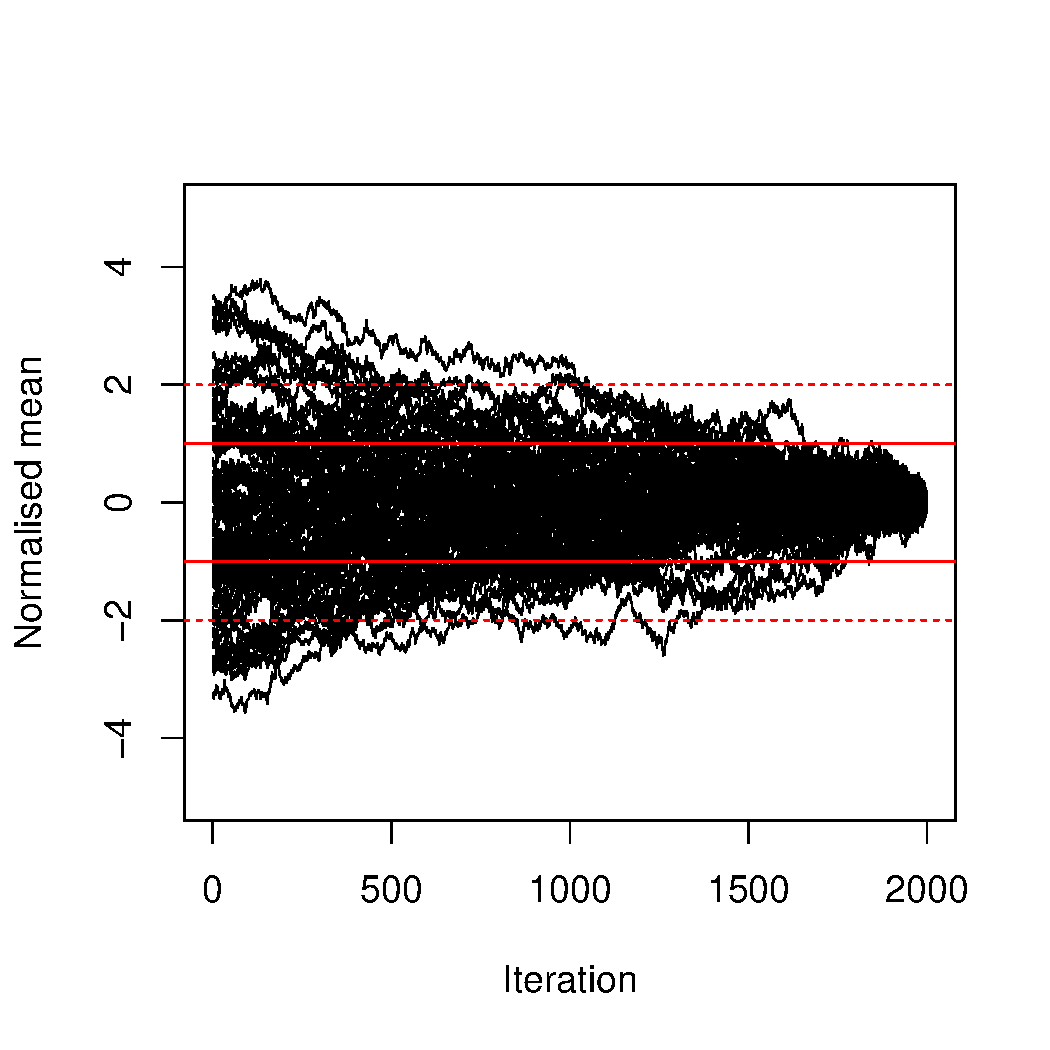
\includegraphics[height=10cm]{background/Figures/AllMeanParticles.pdf}
        \caption{}
        \label{}
    \end{subfigure}
    \begin{subfigure}[t]{\textwidth}
    \centering
      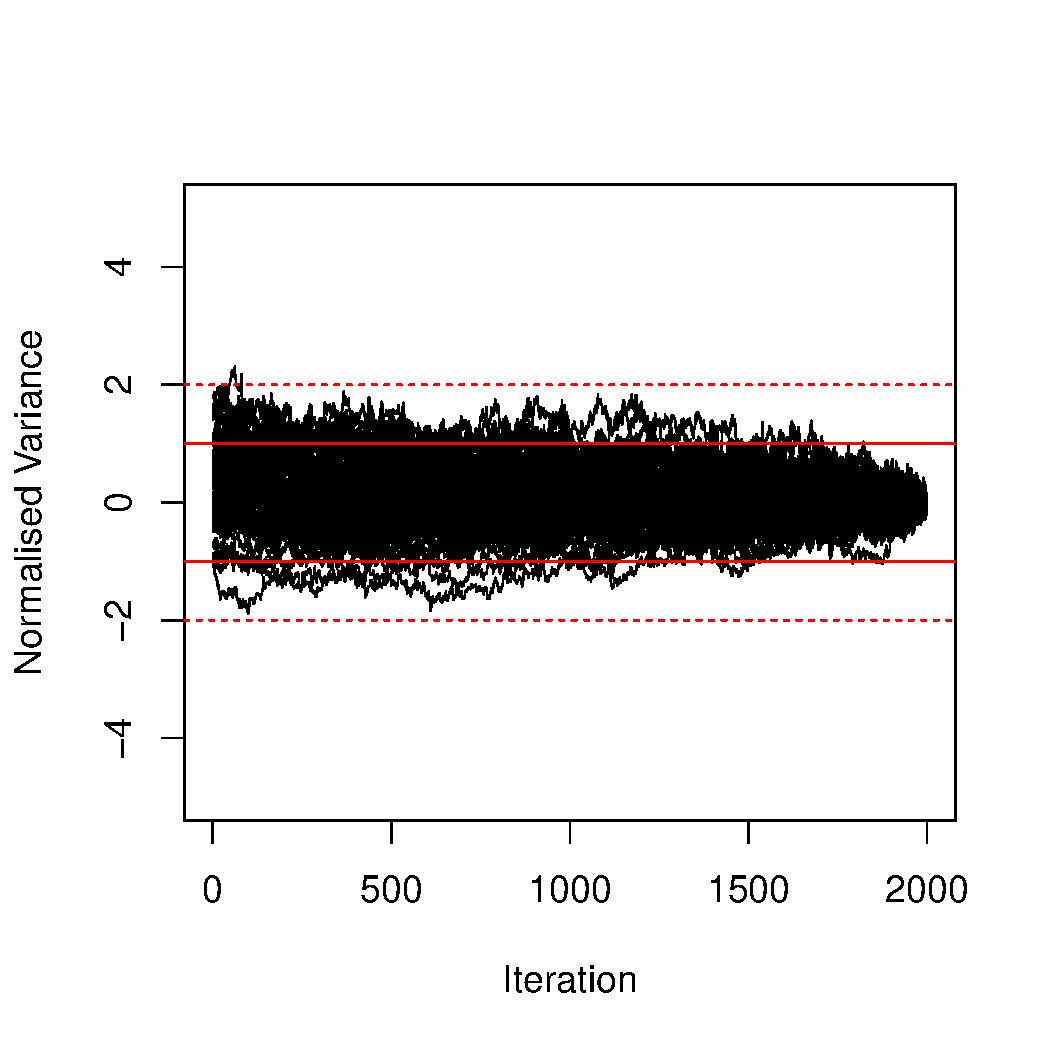
\includegraphics[height=10cm]{background/Figures/AllVarParticles.pdf}
        \caption{}
        \label{} 
    \end{subfigure}
\caption{Normalised mean (a) and variance (b) of each parameter in BHM model as functions of iterations. The normalisation values are the mean and variance of the ensemble of particles positions at the last iteration. Red lines show one and two sigma levels of these normalisation values. Only shown the last 2000 iterations previous to stopping the algorithm.}
\label{fig:convergence}
\end{figure}


Once all parameters have entered the equilibrium state, I stop the \emph{emcee} sampling once the criterium of \citet{Gong2016} \footnote{Implemented in the R package \emph{mcmcse} \citep{mcmcse}} is fulfilled. We chose this criterium because it was developed for high-dimensional problems and tested on Hierarchical Bayesian Models, as in the present work. In this criterium, the MCMC chain stops once its effective sample size (ESS) is larger than a minimum sample size. This minimum is computed using the required accuracy, $\upsilon$, for each parameter confidence interval $(1-\delta)$100\%. The ESS is the size that an independent and identically distributed sample must have to provide the desired accuracy on the parametric inference. 

The \emph{emcee} run stops once the ESS of the ensemble of walkers is greater than the minimum sample size needed for the required accuracy $\epsilon = 0.05$ on the 68\% confidence interval ($\delta = 0.32$) of each parameter.


\section{Codes}
\label{sect:code}
This Section sets out the details about the code I developed to perform the computation described throughout this chapter. First, I give a brief chronological description of the model development. Later, I will describe the details on the implementation of the charged PSO, the modified \emph{emcee}, and the GMM used to describe the field population. Finally, I will end this Section detailing the hybrid high performance computing (Hybrid-HPC) code developed to minimise the computing time of the posterior distribution in the BHM.

The first version of the Bayesian Hierarchical Model was implemented by \'Angel Berihuete in the package \emph{Stan} \citep{Stan}. It comprised a Bayesian model of the ML model of \citet{Sarro2014}. The proper motions were modelled using a single mixture of gaussians. The photometry was modelled with a Chebyshev polynomial parametrised by the length along the sequence. This length was found using a principal curve analysis and lacked physical interpretation.

I took this version and modified in the following aspects. I included the photometric and proper motions EMB sequence, the uncertainties both in proper motion and in photometry, and the width of the sequence modelled as the multivariate gaussian. Then, we realised that the principal curve analysis is not compatible with the deconvolution methodology. The principal curve analysis is driven by the elements with higher variance. Thus, we decided to parametrise the polynomials with the true colour, a more interpretable nuisance parameter that was later marginalised with the aid of a prior. For this prior we introduced the colour distribution as a GMM. 

Previous to the introduction of the marginalisation of the nuisance parameters, the model worked fine on samples of a few hundreds of stars. Once the marginalisation was introduced, the computing time of the model increased dramatically, rendering its application to higher data sizes unpractical. At this point we decided to port the existing \emph{Stan} code into \emph
{Python}\footnote{https://www.python.org} so that we can work with the parallel \emph{emcee} code. \emph{emcee} proved to be of great use. Due to its parallelisation capabilities we were able to increase the data size from 2000 to 10,000 objects. Since the computing of the likelihood was the highest computational challenge, I developed my own routines to perform it on parallel. However, \emph{CosmoHammer} \citep{Akeret2013} turn out to be more efficient in distributing the parallel loads. I ported the BHM code into \emph{CosmoHammer} and modified this last one. The modifications ranged from data files and log entries, to the introduction of priors and the handling of an Hybrid-HPC scheme using both MPI and multithreading. Despite the Hybrid-HPC scheme, the computing of the likelihood of a data set with $10^5$ objects seemed unreachable. At this point, I performed two tasks, the first was to strip the code of all auxiliary libraries calls, and the second was the vectorisation of the majority of the operations. Since the parameters of the field were held fixed, the field likelihood was computed externally for each object. The code was then fed with the data, the field likelihood, and the auxiliary computations reduced at minimum. Among the reduced computation there are, for example, the Cholesky decompositions and matrix inversions of the covariance matrices of the uncertainty. Instead of doing these computation inside the code, the code was fed with the precomputed values. This further reduced the computing time.

Introducing PSO and later the charged PSO reduced even further the computing time.  At this point the code was able to run on a data set with $10^5$ objects. However, convergence of the MCMC still required several weeks of computations. Once the approximation to the marginalisation integral (Eqs. \ref{eq:clmarginalps} and \ref{eq:clmarginalpb}) was introduced, the computing time reduced far more. Finally, the tuning of the \emph{emcee} parameters allowed us to increase the acceptance fraction, and reach convergence within for weeks of full computing time with a 80 cores computer cluster. It is indeed a very long time, however it is reasonable compared with our original estimates of approximately 2 years of computing time.\footnote{Today, the DANCe team is working on a GPU version of the code which is expected to compute the same amount of calculations in a couple of days.}.

\subsection{The modified charged PSO}
\label{sect:chargedPSO}
As explained before, the charged PSO of \citet{Blackwell2002} was inappropriate to our objective. The metric of the parametric space of our problem is not isotropic, parameters have different length scales. For example, while fraction are constrained in the $[0,1]$ interval, proper motions parameters are allowed in the range of proper motion measurements $[-99,99]\,mas\cdot yr^{-1}$. Therefore, the use of an isotropic metric results in a solution which is crowded in some parameters while is over dispersed in others. 
To solve this issue, I modified the charged PSO by measuring distance between particles and applying the electrostatic force independently on each parameter. In such a way, the electrostatic force plays a role only when the relative distance between particles is smaller than $10^{-10}$. I found this value heuristically.

In the original version of  \citet{Blackwell2002}, each particle is subject to the acceleration,
\begin{equation}
\label{eq:PSOacc}
\mathbf{a}=\sum_{i\neq j} \frac{q_i \cdot q_j }{r_{ij}^3} \cdot \mathbf{r}_{ij}, \ \ \ \ p_{core} < r_{ij} < p
\end{equation}
where $q_i$ and $q_j$ are the charges of particles $i$ and $j$, $r_{ij}$ is the distance between them. The distances $p_{core}$ and $p$ indicate the minimum and maximum distances at which the electrostatic force came into action. Outside this range, the electrostatic force is zero. In this equation, $\mathbf{r}_{ij}= \mathbf{x}_i -\mathbf{x}_j$, where $\mathbf{x}_i,\mathbf{x}_j$ are the positions of particles $i$ and $j$. Also, $\mathbf{r}_{ij},\mathbf{x}_i,\mathbf{x}_j \subset \mathbb{R}^d$, with $d$ the dimension of the space. 

In the modified version, the distance is measured independently in each dimension of the parametric space. Thus, $\mathbf{r}_{ij}= \{x_{1,i} -x_{1,j},x_{2,i} -x_{2,j},...,x_{d,i} -x_{d,j}\}$. Also the acceleration has the form,
\begin{equation}
\label{eq:PSOacc}
\mathbf{a}=\sum_{i\neq j} \frac{q_i \cdot q_j }{r_{ij}^2} \cdot \mathbf{r}_{ij}, \ \ \ \  10^{-50} < \frac{r_{ij}}{r_{eq}} < \epsilon
\end{equation}
and it is now applied over each dimension of the parametric space. The distance $r_{eq}$ is that at which the velocity caused by the acceleration equals the mean velocity caused by the common PSO. $\epsilon$ is a free parameter, which as said previously was set heuristically to $10^{-10}$.

\subsection{Improvements of emcee}
The modification I introduced in \emph{emcee}, although very simple, improved the acceptance fraction and mixing of the particles.
To allow the parallelisation, \citet{Foreman2013} divide the ensemble of particles in two ensembles. In the original version, the particles in one ensemble use one and the same particle in complementary ensemble to compute their positions according to Eq. \ref{eq:stretchmove}. In the modified versions, particles from one ensemble update their positions using a particle from the complementary ensemble, however, this particle is chosen randomly at each iteration. 

In a private communication with David Foreman, the developer of \emph{emcee}, he mentions that a similar modification was already introduced in a beta version of \emph{emcee} code.

%Figure \ref{fig:emceeDANCe} compares the mixing and acceptance fractions of the original and modified versions of \emph{emcee}.
%\begin{figure}[htbp]
%\begin{center}
%%\includegraphics[width=\textwidth]{}
%\caption{Comparison between the log posterior evaluations of the original emcee version (left) and the modified one (right). }
%\label{fig:emceeDANCe}
%\end{center}
%\end{figure}
\subsection{GMM for the field population}
As mentioned earlier in this Chapter, the field population is modelled by means of two independent photometric and proper motion distributions. The MLE of the parameters of these distributions were found using the EM algorithm.  The conventional EM algorithm for GMM \citep{Dempster1977} for a mixture of $M$ gaussians goes as follows. Given a set of parameters $\theta=\{w_i,\boldsymbol{\mu}_i,\boldsymbol{\Sigma}_i\}_{i=1}^M$, were $w_i$,$\boldsymbol{\mu}_i$, and $\boldsymbol{\Sigma}_i$ are the fraction, mean and covariance matrix of gaussian component $i$, the likelihood of the data is,

\begin{equation}
p(\{\mathbf{y}_n\}_{n=1}^N|\theta)=\prod_{n=1}^N {\sum_{i=1} ^M {w_i\cdot \mathcal{N}(\mathbf{y}_n|\boldsymbol{\mu}_i,\boldsymbol{\Sigma}_i)}}.
\end{equation}

To solve the problem, the EM algorithm requires  a set of $N$ variables, $\{\boldsymbol{z}_n\}_{n=1}^N$, of dimension $M$. The variable $z_{n,i}$ represent the probability that observation $y_n$ was drawn from gaussian $i$. Therefore,

\begin{equation}
1=\sum_{i=1}^M z_{n,i}.
\end{equation}

These $\boldsymbol{z}$ latent variables are found as
\begin{equation}
z_{n,i}= \frac{w_i\cdot \mathcal{N}(\mathbf{y}_n|\boldsymbol{\mu}_i,\boldsymbol{\Sigma}_i)}{\sum_{i=1}^M w_i\cdot \mathcal{N}(\mathbf{y}_n|\boldsymbol{\mu}_i,\boldsymbol{\Sigma}_i)}.
\end{equation}

The EM works, as its name indicates, by maximising the expected value of the likelihood. This last is given by
\begin{equation}
E[p(\{\mathbf{y}_n\}_{n=1}^N|\theta)]=\prod_{n=1}^N {\sum_{i=1} ^M {z_{n,i}\cdot w_i\cdot \mathcal{N}(\mathbf{y}_n|\boldsymbol{\mu}_i,\boldsymbol{\Sigma}_i)}}.
\end{equation}

The previous expectation is maximal when,
\begin{align}
w_i &= \frac{1}{N} \sum_{n=1}^N z_{n,i}, \\
\boldsymbol{\mu}_i &= \frac{1}{\sum_{n=1}^N z_{n,i}} \sum_{n=1}^N z_{n,i}\cdot \mathbf{y}_n,\\
\boldsymbol{\Sigma}_i &= \frac{1}{\sum_{n=1}^N z_{n,i}} \sum_{n=1}^N z_{n,i}\cdot (\mathbf{y}_n - \boldsymbol{\mu}_i)\times(\mathbf{y}_n-\boldsymbol{\mu}_i)^T.
\end{align}

The modified version of the GMM, which includes a uniform distribution, is now a particular case of the GMM. This can be viewed as a gaussian distribution with fixed parameters and a constant probability $c$ given by the uniform distribution. The new expectation is then,
\begin{equation}
E[p(\{\mathbf{y}_n\}_{n=1}^N|\theta)]=\prod_{n=1}^N {\left[z_{n,0}\cdot w_0 \cdot c + \sum_{i=1} ^M {z_{n,i}\cdot w_i\cdot \mathcal{N}(\mathbf{y}_n|\boldsymbol{\mu}_i,\boldsymbol{\Sigma}_i)}\right]}.
\end{equation}

The maximisation step remains identical except for the indices. There are now $M+1$ fractions $w_i$, with $i=0,1,...,M$, and the means and covariances run from $i=1,...,M$.

Regarding the photometric GMM of the field. Since photometry has missing values, we use the EM algorithm of \citet{McMichael1996}. This algorithm was developed to obtain the MLE of data with missing values. A more recent version has been developed by \citet{Lin2006}, however, this assumes that the missing data is randomly distributed (missing at random). However,  as mentioned earlier, the missing values in the photometry of the DANCE DR2 are not randomly distributed.

In the algorithm of \citet{McMichael1996}, there is a set of $N$ gain matrices, one for each datum. Each $M_n$ matrix is an identity matrix in which the rows of the corresponding missing value have been deleted. Thus, the expected value of the likelihood is now,

\begin{equation}
E[p(\{\mathbf{y}_n\}_{n=1}^N|\theta)]=\prod_{n=1}^N {\sum_{i=1} ^M {z_{n,i}\cdot w_i\cdot \mathcal{N}(\mathbf{y}_n|M_n \boldsymbol{\mu}_i,M_n\boldsymbol{\Sigma}_i M_n)}}.
\end{equation}

The maximisation step is now,

\begin{align}
w_i &= \frac{1}{N} \sum_{n=1}^N z_{n,i}, \\
\boldsymbol{\mu}_i &= \frac{ \sum_{n=1}^N z_{n,i}\cdot H_n \mathbf{y}_n}{\sum_{n=1}^N z_{n,i} H_n M_n}
\end{align}
with 
\begin{equation}
H_i=M_i^T(M\Sigma_i M^T)^{-1}
\end{equation}

The maximisation step has no analytical solution for the covariance matrix, therefore, a modified steepest descent is used

\begin{equation}
\Sigma_i \leftarrow \Sigma_i + \frac{\rho}{2}\cdot \Sigma_i\Delta_i\Sigma_i,
\end{equation}
with  and $\Delta_i$ given by

\begin{equation}
\Delta_i=  \frac{1}{\sum_{n=1}^N z_{n,i}}\cdot \sum_{n=1}^N z_{n,i} \cdot \left[H_n(\mathbf{y}_n -  M_n \boldsymbol{\mu}_i) \times  (\mathbf{y}_n -  M_n \boldsymbol{\mu}_i)^TH_n^T - H_nI\right].
\end{equation}
 
 This algorithm preserves the monotonic convergence of the conventional EM, and returns positive definite matrices provided that $\rho < 2$. For details and validation of this algorithm see \citet{McMichael1996}.

\subsection{Hybrid-HPC implementations}
\label{sect:HHPC}
As I outlined before, the parallel computing approach was an unavoidable step. Once the code was ported to \emph{Python} and \emph{CosmoHammer}, I modified this last one to better fit our needs. The modifications were mainly on the management of input and output files and the python \emph{multiprocessing} package for the multithreading computing of likelihood. Also, I striped some of its original functions to reduce memory usage and implemented some others, like the use of initial positions for the particles.

In the Hybrid-HPC approach, the particles of \emph{emcee} are distributed on the nodes of the computing cluster by means of the MPI protocol. Then, each core in the node computes the likelihood of one fraction of the objects in the data set. This Hybrid-HPC code was implemented and tested in different computing cluster architectures. For the cluster at the Centre of Astrobiology (CAB, Villanueva de la ca\~nada, Madrid,Spain), I used a configuration of 6 nodes each with 12 cores. For the cluster at the University of C\'adiz, (Andaluc\'i
a, Spain) I used a configuration of 5 nodes each with 16 cores.

However, the  Hybrid-HPC approach was not the best solution at the CIMENT clusters of the University of Grenoble Alpes. At this cluster (I used Froggy), the code continuously render errors of communication. For this reason, I implemented a only-MPI version of the code. In this version, the multithreading approach is left aside. Instead, the totality of the available cores is fully dedicated to the computing of the likelihood. Each of the $n$ cores computes the likelihood of one $n$th of the objects in the data set. Once the likelihood of all particles has been computed, the master node evaluates the new positions of the particles.

I finish this chapter with a brief description of the difficulties faced on the development and testing of the BHM code. As the code evolved in complexity, my computational skills were compelled to evolve as well. I started by learning R and solving some toy problems on it. Later, when the dimensionality of the posterior increased I learned \emph{Stan}. When the data set increased in size, we faced the parallelisation, so I learned Python and MPI. Once these versions were operable, I was forced to deal with libraries, from the common, numpy, scipy and numba, to the linking of modules and libraries. Finally, when dealing with several clusters I learned the queue languages Condor, slurm and OAR. Currently, I am working on the improvement (memory allocation and data distribution) of GPU implementation of the BHM code.  




%!TEX root = ../thesis.tex
\chapter{Results}
\label{chap:Results}
In this Chapter I present the results of applying the methodology explained in Chapter \ref{chap:BHM} to the Pleiades DANCe data set (Sect. \ref{sect:DR2}). However, to characterise the methodology and estimate its precision and accuracy, I first apply it over synthetic data. Using this data, I am able to analyse the performance of the methodology when it is considered only as a classifier. Later, in this Chapetr I give the results of our methodology main objective: the statistical characterisation of the cluster population. In the following Sections I give the details of the spatial, velocity, luminosity and mass distributions. Later, I will describe the physical scenario of the evolution of the mass distribution by comparing the Pleiades mass distribution with other younger and older clusters. Finally, I will end this Chapter with a description of how the Bayesian methodology allowed us to update our previous knowledge of the Pleiades cluster.

\section{Performance of the classifier}
\label{sect:classifier}
As mentioned earlier, the main objective of our the methodology of the BHM is the statistical characterisation of the NYOC populations. As a by product, it also obtains individual membership probability distributions. Using these last ones, we are able to directly classify objects into cluster and field members, providing that and objective probability threshold has been stablished. The objective of this section is to find this objective threshold by means of synthetic data. As any other measured property, this classification has an uncertainty, thus, the purpose of this section is also to quantify this uncertainty. 

That said, in order to properly characterise our classifier, I test it over synthetic data sets that resemble the real data. An ideal test to our classifier will be to apply it over well known dataset in which tags of cluster and field members were already present. However, if we may have access to these tags, a classifier may not be needed. The Pleiades cluster being \emph{the} most studied cluster in history, is the  NYOC with most of these tags. This is the reason for which we decided to benchmark our methodology on it. Nevertheless, the problem of the synthetic data remains since the low-mass end of the cluster still is \emph{terra ignota}. To over come this issue, we decided to create synthetic data sets under the assumption that our cluster and field models resemble the real data.  We are aware that these models are far from perfect, but so far is the best we can do. 

The assumption that our model correctly models the real data, although enable us to measure the uncertainty of our classifiers, does not give any indication about possible biases in our model. To explore this possibility, we later compare our real data results with those found in the literature. I present this comparison at the end of this section.

Hence, we fit our models, field and cluster, to the real data ($10^4$) and using the MAP estimates, we created synthetic stars (five samples of $10^4$ objects each). To further test the reliability of our classifier, we compare the results it render when applied over data sets with and without missing values. This comparison allows us to quantify the impact that missing values have on our results.    

One further consideration. The synthetic analysis requires at least three runs: one on the real data to obtain the MAP, and two on the synthetic one: with and without missing values. However, as explained in Chapter \ref{chap:BHM}, our methodology is computationally expensive. Therefore, to maintain the computing time within reasonable limits (couple of weeks), we decided to restrict our synthetic data set to only the $10^4$ objects with higher membership probability according to \citet{Bouy2015}. I elaborate on the consequences of this decision.

These $10^4$ objects are "closer" to the cluster in the sense of membership probability than the remaining 9$\times 10^4$ objects. Therefore, the field probability density rendered by this sample, compared to that of the larger $10^5$ sample, has the following properties: it is more concentrated and has larger values near the cluster region. Since the $10^5$ sample is largely dominated by the field population, its density peaks far form the cluster proper motion and photometric sequences. Densities are normalised, thus more of the density mass of this large sample is far from the cluster region. 

Given the previous considerations, we assume that results obtained on the smaller $10^4$ sample have are more contaminated, and have lower recovery rates than those obtained on the larger and more distant $10^5$ sample. On the one hand, the higher contamination rate results from the larger concentration of the field density around the cluster region.  On the other hand, the lower recovery rates arises from the higher values of the field probability density. In simple words, when we define the field in a more restricted region around the cluster, both populations become more entangled, thus they become more difficult to separate. Therefore, we assume that the results obtained on the smaller $10^4$ sample represent upper and lower limits to the contamination and recovery rates of the larger $10^5$ sample, respectively.

Briefly, to create the synthetic data set, the procedure is the following. First, using the methodology of the previous Chapter, I obtain a sample of the posterior distribution of the parameters given the $10^4$ real data set. Then, I chose the particle with highest posterior probability as the MAP estimate of the posterior distribution. Using this particle positions I generate five synthetic data sets of $10^4$ objects each. Then, I tag these objects according to their parent population: cluster or field. Then, using the synthetically observed values I estimate their uncertainties and missing value patterns (more details  below). Finally, I run the model over these five synthetic samples and compare the measured tags with the true ones as function of the probability threshold.

 Also, I run the methodology over the synthetic data set without missing values and compare this results with those found on the same data set with missing values. This test, as mentioned before, enable us to quantify the impact of missing values over individual membership probabilities.  

As explained in Sect. \ref{sect:DR2}, our data set has a high fraction of missing values. Only $\sim1\%$ has completely observed entries. Furthermore, the missing pattern is not random and depends on the magnitudes and colours of the objects. Therefore, to better reproduce this pattern, for each synthetic datum, we use missing value template of one of its closer neighbours in the real data; closer in the euclidean sense. Using the missing value template of the nearest neighbour from the real data set results in a biased sample in which objects with complete (non missing) values are underestimated. This is the inevitable consequence of the fact that euclidean distances measured in subspaces resulting from the missing values, are smaller or, at most, equal to those measured in the non-missing value spaces. 

Missing values are assigned as follows. Since by definition of our data set there are no missing values in our proper motion data, missing values were assigned only to photometry. We chose the closer neighbours from the available CMDs: $\{K_s,J-K_s\},\{J,J-H\},\{K_s,H-K_s\},\{J,Y-J\},\{K_s,i-K_s\}$. These CMD are formed with the bands and colours with fewer missing values, in decreasing order.  The missing value pattern for individual objects was chosen as follows. First, for each CMD subspace we find the fraction, $f_r$, of objects from real data without missing values, we call it $C_{or,i}$. Then, we take a random sample from the synthetic data whose fraction, $f_s$ corresponds to $f_r$. For objects in this sample we assign the missing value pattern of the nearest neighbour from sample $C_{or,i}$. We repeat the procedure for all CMDs. In this way, the synthetic data has fractions of missing and non-missing values similar to those of the real data.

Uncertainties are assigned as follows. We set the proper motions uncertainties to those of the nearest neighbour in the real data. In photometry, however, this scheme renders uncertainties that are biased towards the less precise measurements. This is a consequence of the missing values. Again, the euclidean metric results in the preferential choosing of objects with missing values. These missing values occur mostly at the faint end, where uncertainties are larger. Therefore, the uncertainties are biased towards larger values. To avoid this issue, we fit polynomials (8th degree) to the uncertainties as a function of the magnitudes. Then, we use these polynomials to give uncertainties to the synthetic photometric data.

The performance of our classifier was measured by counting the true positives (TP, cluster members correctly classified), true negatives (TN, field members correctly classified), false positives (FP, field members classified as cluster members) and false negatives (FN, cluster members classified as field members) recoveries as a function of the probability threshold. With them we calculate the true positive rate, contamination rate, accuracy and precision, which are defined as follows. In order to classify the objects as cluster of field members we summarise their membership probability distribution using the mode. If the mode is grater than the current probability threshold, then the object is classified as cluster member, if not as field.

The true positive rate (TPR) is the ratio of true positives over the sum of true positives plus false negatives. The contamination rate (CR) is the ratio of false positives over the sum of false positives plus true positives. The precision or positive predictive value (PPV) is the ratio of true positives over the sum of true positives plus false positives. Finally, the accuracy (ACC) is the ratio of the sum of true positives plus true negative over the sum of true and false positives and negatives. These are,

\begin{align}
TPR &= \frac{TP}{TP+FN} \nonumber \\
CR   &= \frac{FP}{FP+TP} \nonumber \\
PPV &= \frac{TP}{TP+FP} \nonumber \\
ACC &= \frac{TP+TN}{TN+FN+TP+FP} \nonumber
\end{align}

We use the results of the five synthetic data sets to quantify the uncertainties of the previous quantities. 

In Fig. \ref{fig:tfpr} I show the TPR and CR, as a function of probability threshold, computed for the cases in which missing values where both present and absent. The missing value case was computed for the five synthetic samples, thus, the lines and the shaded grey regions depict the mean and maximal deviations, of the results found on the five synthetic samples. As can be seen in this Figure, the missing values have a negative impact in our classification. They cause a diminishing of the TPR  and an increase in the CR. This negative impact is expected since the observables we are using are highly discriminant in the classification process. Since cluster and field are highly entangled in our $10^4$ synthetic samples, when a highly discriminant observable is missing the classification process could be biased or more uncertain.

In spite of the negative impact of missing values, our methodology delivers low ($\lesssim 8\%$) contamination rates and high recovery rates. In Figure \ref{fig:tfpr} we also show , for the sake of comparison, the CR and TPR of \citet{Sarro2014} (reported in their Table 4). 

From the previous comparison we observe that the TPR delivered by of our methodology: i) when measured on data without missing values, is similar to that of \citet{Sarro2014} methodology. This is expected since the results of those authors are based on a model constructed only with completely observed objects (i.e. non-missing values). ii) when measured on data with missing values, is $\approx 4\%$ lower than that of \citet{Sarro2014}. 

This last figure is a small price to pay compared to the dramatical increase in the number of sources used to construct our model (both field and cluster). As mentioned in Section \ref{sect:DR2}, in our $10^5$ objects data set, only $\sim 1\%$ of objects have completely observed entries. Roughly, this is the fraction of sources used by \citet{Sarro2014} and \citet{Bouy2015} to construct their models. 

On the other hand, the CR of our methodology, above $p=0.8$ and for both missing-values and non-missing values cases, outperform, by $x\%$, the CR reported of \citet{Sarro2014} methodology, see below.

In simple words, what can be observed from the previous analysis is that our methodology, compared to that of \citet{Sarro2014}, renders less contaminated (CR) results ($x\%$) at the price of a smaller recovery rate (TPR) $4\%$

Nonetheless, we stress the fact that the previous comparison is not straight forward. The following reasons must be born in mind. First, \citet{Sarro2014} infer their cluster model using only non-missing-value objects, later they apply that model to objects with and without missing values. Second, their synthetic data set and ours are essentially different. They are constructed with different generative models, different number of elements, and different missing value patterns. 

Now, I describe the procedure to set an objective probability threshold. This probability threshold, although is not needed to obtain the distribution of the cluster population, is needed however to objectively classify an object. Since real data contain missing values, there is no need establish this threshold for the non-missing values case. There are different approaches to establish this probability threshold, however I only use the approach of maximum accuracy (ACC). 

Figure \ref{fig:tfpr} shows the ACC and the PPV of our classifier when applied on synthetic data with missing values. The lines and the grey regions depict, respectively, the mean and the maximum deviations of the five synthetic data set results. We use these last ones as the uncertainty of our estimates. The mean of the highest accuracy, ACC=$96.5\pm0.1$\%, happens at probability threshold $p_t = 0.84$. At this threshold the CR is $4.3\pm0.2$\%, the TPR is $90.0\pm0.05$\%, the ACC is , and the PPV is $95.6\pm0.2$\%. 

\begin{figure*}[!htp]
\begin{center}
%\resizebox{\hsize}{!}{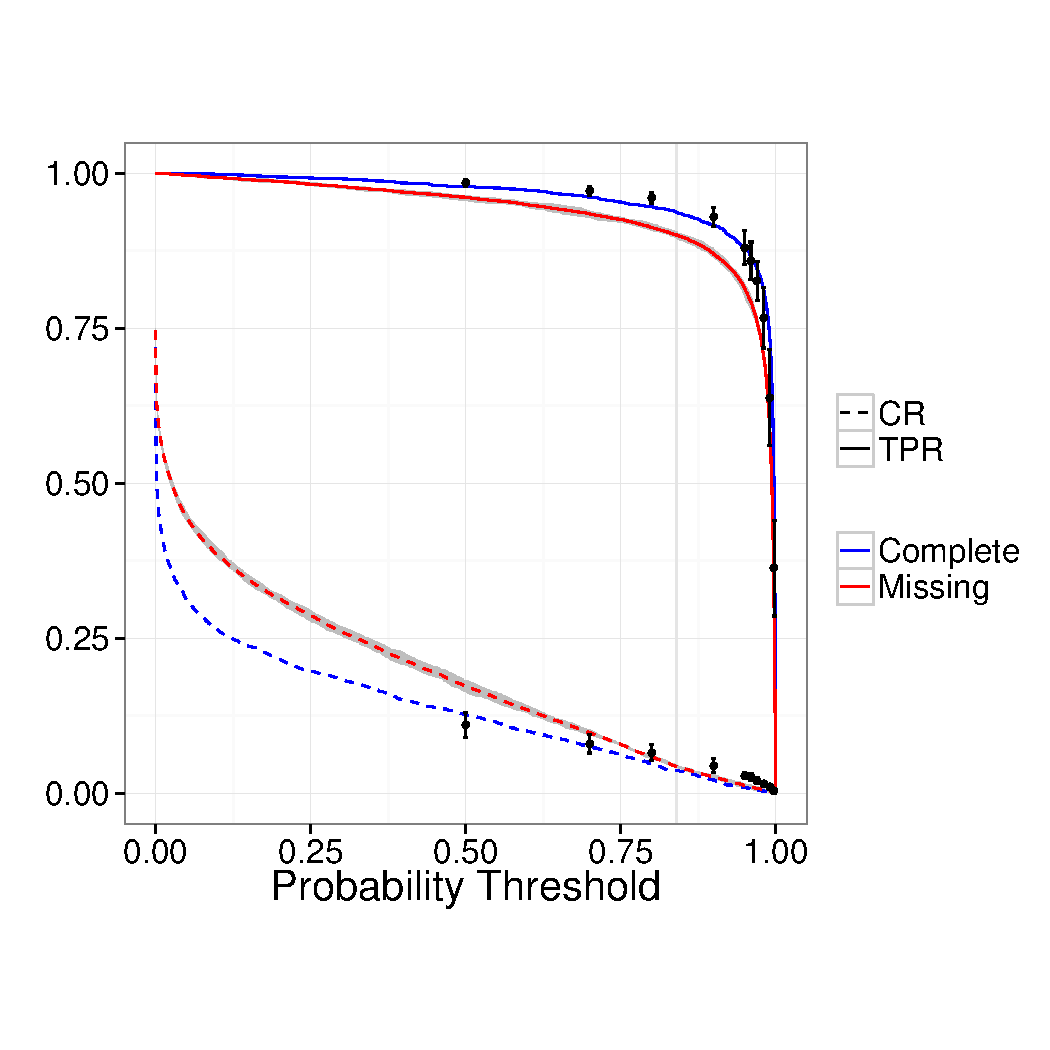
\includegraphics{figs/FTPRvsSarro.pdf}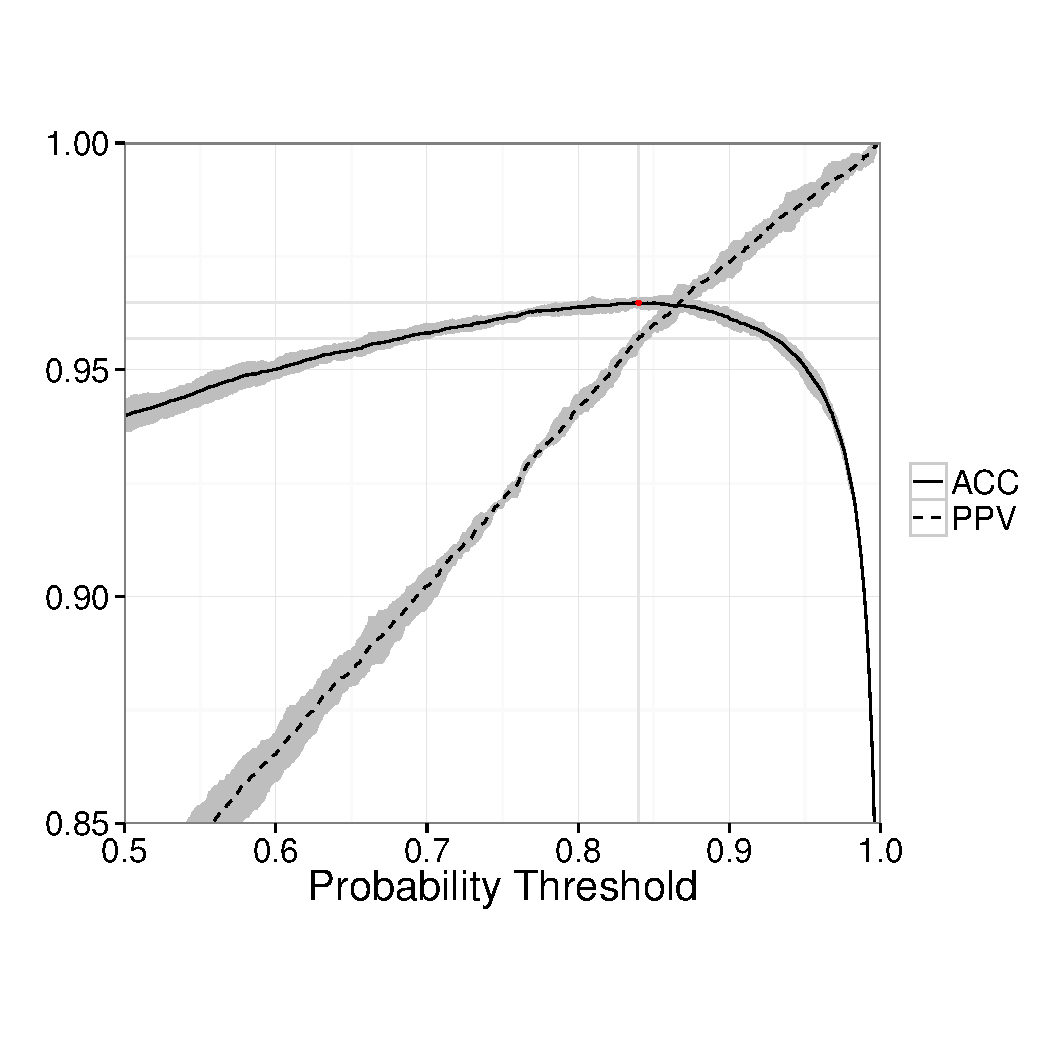
\includegraphics{figs/PrecisionAccuracy.pdf}}
\caption{Left: The TPR (solid line) and CR (dashed line) of our methodology  when applied on synthetic data sets with and without missing values (red and blue lines, respectively). In black dots we show the TPR and CR reported by \citet{Sarro2014} for their non-missing values model. Right: Accuracy and precision as a function of probability threshold for our classifier when applied on synthetic data with missing values. The higher accuracy is obtained at $p_t=0.84$ (red dot). In both panels, the grey areas show the maximum deviations from the mean of the results of the five missing-values synthetic data sets.}
\label{fig:tfpr}
\end{center}
\end{figure*}

We investigate further on the impact of missing values, particularly to analyse any possible biases introduced by them. It was done by comparing the mode of the individual membership probability distributions found after fitting the model to data sets with and without missing values. The missing values data set is the result of adding a mask of missing values (as previously described) to the completely observed data set. It means that this data set has identical observed values, except for those masked as missing ones. 

In Fig. \ref{figure:IncVsCom} we show the mode of the membership probabilities of objects with missing values (vertical axis) against those of non-missing values (horizontal axis). As can be seen in this Fig., the missing values impact our results by spreading the membership probabilities. Ideally, we would like to recover membership probabilities following the line of slope one, as in the case of completely observed values (red squares). The most striking deviations come from objects lacking the $CI$ (enclosed in black). Our methodology uses the \emph{true} $CI$ to prescribe the \emph{true} photometry, and the observed $CI$ to constrain the marginalisation integral of the \emph{true} $CI$. Thus, it is expected that a missing $CI$ will produce a probability spread. These missing $CI$ objects show two different behaviours. In one case, there are sources with membership probabilities $p_{complete} \approx0$ which have overestimated probabilities in the incomplete case (vertical axis). In the other case, the sources in the combed area below the line of unit slope have underestimated probabilities in the incomplete case. While the first case contributes to the CR the second one diminishes the TPR. The first case reaches the maximum difference at $p \approx 0$ (difference between red and blue dashed lines in Fig. \ref{fig:tfpr}), thus its impact in our results is marginal. Furthermore, at our objective probability threshold $p_t=0.84$, these objects have a small impact in our results, they represent only 1.8\% of the contamination rate. The box region in Fig. \ref{figure:IncVsCom} shows them. The second case, however, typify the unavoidable loss of members due to the missing values, 4\% at $p_t=0.84$, given our model and the observables it uses.


The bias introduced by missing values can be estimated using the root-mean-square (rms) of the difference between membership probabilities recovered with and without missing values. The total rms is 0.12. On the one hand, objects with completely observed values (red squares) in both data sets have a rms of only 0.02. On the other hand, objects with missing values have a rms of X. While the rms of objects lacking the $CI$ have and rms of X.  The previous effects show an overall agreement between results on data sets with and without the missing values, nonetheless, care must be taken when dealing individually with objects lacking the $CI$. 


As mentioned before, our methodology aims at the statistical distributions of the cluster population. It works by ensuring that each object contributes to the cluster distributions proportionally to its cluster membership probability. In this sense our results are free of any possible bias introduced by hard cuts in the membership probability. Nevertheless, contamination is still present and must be quantified. To quantify it, I compute the expected value of the CR. It is $\langle CR \rangle=5.8\pm 0.2$\%. In this expected value, each CR contributes proportionally to the  probability threshold at which it is measured. 

\begin{figure}[!htp]
\begin{center}
%\resizebox{\hsize}{!}{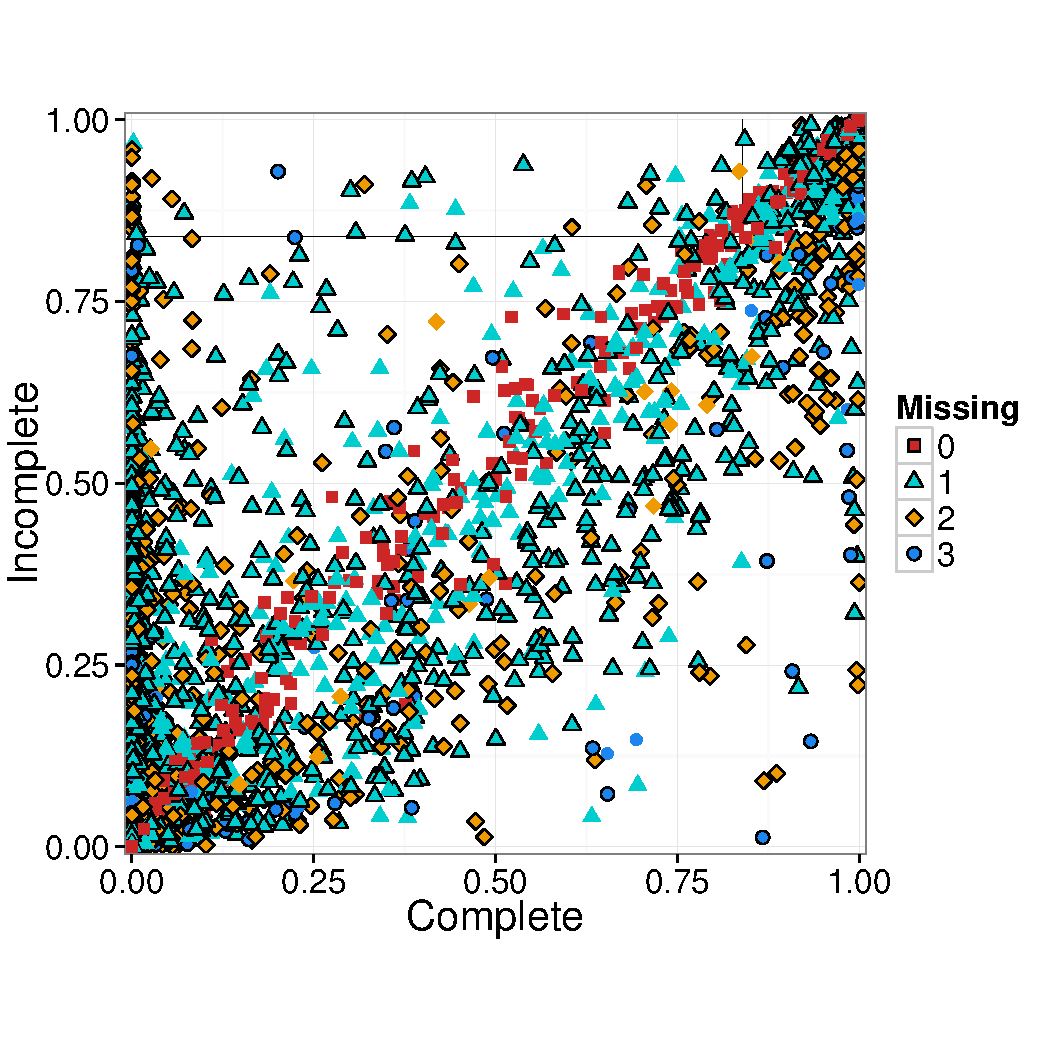
\includegraphics[page=1]{figs/Probabilities.pdf}}
\caption{Comparison between the cluster membership probabilities recovered from the synthetic data with missing values (Incomplete) and without them (Complete). The colour and shape indicate the amount of missing values. The symbols enclosed in black indicate a missing $CI$. The top left box contains objects considered as contaminants due to missing values, at the probability threshold $p_t=0.84$.}
\label{figure:IncVsCom}
\end{center}
\end{figure}

In machine learning and data mining is sometimes useful to analyse the performance of a binary classifier by the receiver operating characteristic curve, the ROC curve.  This plot is a visual diagnostic of the ability of a classifier to to its job. The ROC curve plots the TPR as a function of the FPR for all possible values of the probability threshold. A perfect classifier would be that in which the TPR=1 and the FPR=0 for some probability threshold. On the other hand, a random classifier would be that on which the TPR=FPR at all probability thresholds. Such classifier has a line of slope one as its ROC curve. Furthermore, the quantitative diagnostic for a binary classifier is the area under the ROC curve (AUC). As its name indicate, the AUC is the integral of the ROC curve. Thus a random classifier has a AUC of one half, while a perfect classifier as AUC=1. In Fig. \ref{fig:ROC}, I show the ROC curve for our classifier when applied over synthetic data with missing values. It is the ROC of one of the five synthetic realisations described throughout this section. As can bee seen from this Fig. our classifier does an excellent job, with an AUC=0.99.

\begin{figure}[!htp]
\begin{center}
%\resizebox{\hsize}{!}{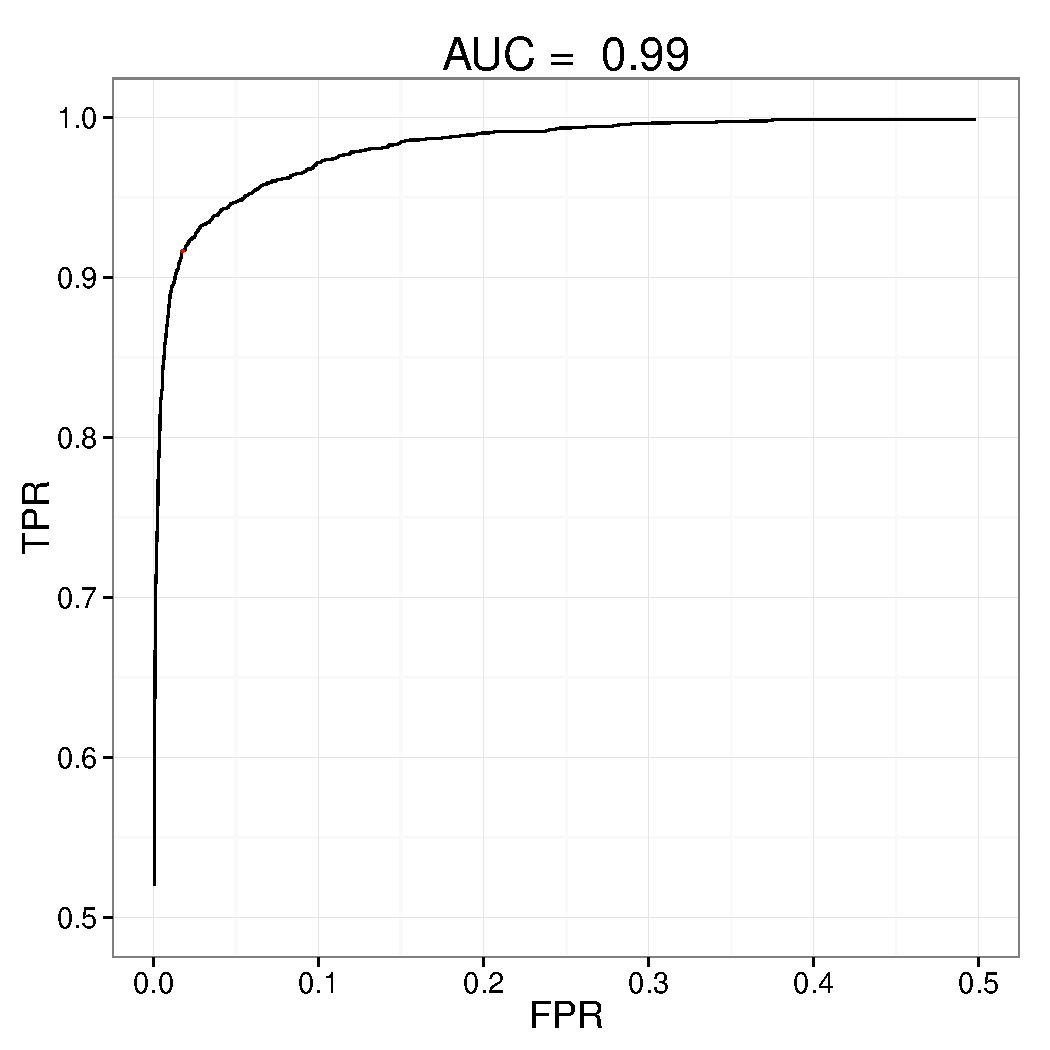
\includegraphics[page=1]{figs/ROC.pdf}}
\caption{ROC curve of our classifier when applied over one of the synthetic data sets described earlier. As can be seen the AUC=0.99 diagnose it as an excellent classifier.}
\label{fig:ROC}
\end{center}
\end{figure}

 
\subsection{Comparison with the literature}
In Chap. \ref{chap:pleiades} I mentioned that the most important works on the Pleiades members are those of \citet{Stauffer2007,Lodieu2012,Sarro2014,Bouy2015}. In this section I will compare the list of candidate I members found with the most recent study of the Pleiades members, that of \citet{Bouy2015}. Later, for the sake of completeness, I will compare my list of candidate members with the compilation made by \citet{Stauffer2007}.  

\subsubsection{Candidate members from \citet{Bouy2015}}
\label{sect:comparisonBouy}
The methodology of this work, although essentially different from that of \citet{Bouy2015}, the fact that both share the data set and use the same observables, allows a direct comparison between them. When using their objective probability thresholds, as shown by Fig. \ref{figure:HM-SBB}, both methodologies agree on the outstanding $99.6$\% of the classified objects. Concerning the candidate members, they also agree on $\approx 90\%$ of them. Nevertheless, the discrepancies are worthy of discussion.

The rejected candidates of \citet{Bouy2015} (lower right box of Fig. \ref{figure:HM-SBB}) amount to 12\% of their total number of candidate members. This value is 4.7\% higher than the contamination rate reported by \citet{Sarro2014}: $7.3\pm1.4$\%. I will not reject a priori these objects as candidate members because, as mentioned in Sect. \ref{sect:classifier}, our methodology recovers 4\% less members when compared to that of \citet{Sarro2014}(see Fig. \ref{fig:tfpr}). The majority, $85\%$, of these objects have missing values, which indicates that these objects require future follow up. Even the 37 completely observed and rejected candidates can not be discarded as true members due to the fact that our methodology losses 6\% of the true cluster members (see Fig. \ref{fig:tfpr}).  

On the other hand, our new candidates (upper left box of Fig. \ref{figure:HM-SBB} ) amount to 10\% of \citet{Bouy2015} candidates. This figure is higher than the $4.3\pm0.2$\% CR reported on the previous Section. Thus, it indicates that up to $\sim6\%$ of these objects can be true cluster members. From these objects, one half have completely observed values, thus 3\% of our new candidates are completely observed objects. This las figure agrees perfectly well with the 3\% of non recovered members reported by \citet{Sarro2014}. 

In Figs. \ref{figure:newones} and \ref{figure:rejecteds} I show the proper motions and $K_s$ vs $i-K_s$ CMD projection spaces of our new candidates and the rejected ones  of \citet{Bouy2015}. In the following I elaborate on their properties.

The new candidate members have proper motions uncertainties whose median, $\overline{\mu_{\alpha,\delta}}=\{1.33,1.33\} \ \ mas/yr$, is two times larger than those of the candidate members in common with \citet{Bouy2015}, median $\overline{\mu_{\alpha,\delta}}=\{0.65,0.65\} \ \ mas/yr$. Also, as shown by Fig. \ref{figure:newones}, the majority of the new candidate members, 148, have probabilities lower than 0.95, are located in a halo around the locus of the cluster proper motions, and on top of the cluster sequence in the $K_s$ vs $i-K_s$ CMD. On the contrary, the new candidates with probabilities higher than 0.95, which are 39, lay in the centre of the cluster proper motions and fall above the cluster sequence in the $K_s$ vs $i-K_s$ CMD. Thus, I hypothesise that: i) Objects whose photometry is compatible with the cluster sequence but are in the proper motions halo, have higher membership probabilities in our methodology due to the increased flexibility of the cluster proper motions model: it now has four gaussians instead of the two of \citet{Bouy2015}. And ii) objects near the centre of the cluster proper motions but located above the cluster photometric sequence sequence, are multiple systems \cite[probably triple systems which can amount to 4\% of the population][]{Duquennoy1991} with an increased membership probability due to our more flexible photometric model of the cluster and equal-mass binaries sequences.

The rejected candidates of \citet{Bouy2015}, as it is shown in Figs. \ref{figure:rejecteds} and \ref{figure:rejectedsCOLORS}, have proper motions uncertainties with median $\overline{\mu_{\alpha,\delta}}=\{3.15,3.19\} \ \ mas/yr$. This value is more than four times larger than that of the candidates in common with our members. Also, these objects are distributed along the cluster sequence. Among these objects, those with a relatively high membership probability occur mostly at the middle of the cluster sequence (green squares of Fig. \ref{figure:rejectedsCOLORS}) while those with lower membership probabilities occur at the bright and faint ends (blue and red triangles of Fig. \ref{figure:rejectedsCOLORS}, respectively). These last regions coincide with those where the missing values happen the most. We stress the fact that \citet{Sarro2014} and later \citet{Bouy2015} construct their models using only completely observed objects (i.e. those without missing values). For their field models both authors use a sample of $\approx 20,000$ objects. Proceeding in that way, as explained in Sect. \ref{sect:missing}, underestimates the field density, particularly in the regions where the missing values are more frequent. Underestimating the field likelihood increases in the cluster field likelihood ratio, therefore it increases also the cluster membership probabilities. Furthermore, the proper motions uncertainties of objects at the bright middle and fain ends, have medians of $\overline{\mu_{\alpha,\delta}}=\{4.0,4.2\} \ \ mas/yr$, $\overline{\mu_{\alpha,\delta}}=\{2.4,2.4\} \ \ mas/yr$ and $\overline{\mu_{\alpha,\delta}}=\{3.4,3.4\} \ \ mas/yr$, respectively. These figures are approximately 6, 4 and 5 times larger, respectively, than those of the candidates in common. These large uncertainties produce a proportional spread of the likelihood distribution thus further reducing the membership probability.

I consider that both the large proper motion uncertainties and field likelihoods are responsible for the diminished membership probabilities of \citet{Bouy2015} rejected candidates. However, these rejected candidate members cannot be discarded as potential members. Indeed, at the probability threshold of maximum accuracy, $p_t=0.84$, the TPR is just $90.0\pm0.05$\%. It means that there are still 10\% of true members within the rejected candidates. To rule out the possibility that these objects are indeed members we need lower proper motion uncertainties and fewer missing values. Future steps will be taken to try to solve this issue.

Summarising, the discrepancies between our individual membership probabilities and those reported by \citet{Bouy2015} arise from subtle but important differences. The first of them is the more formal treatment of missing values in our methodology and its inclusion in the field model. Taking into account the missing values has two main consequences. The first of them is that, the new photometric model of the field diminished membership probabilities, particularly in the regions where missing values happen the most. Second, the use of missing values in the construction of the cluster model allow us to include the information of good candidate members that were otherwise discarded a priori. The second difference is the higher flexibility of our cluster model, it allows us to increase the membership probability of the previously discarded candidates. Furthermore, as shown by the red squares in the upper left corner of Fig. \ref{figure:HM-SBB}, the higher flexibility of our cluster model allow us to include as new candidate members previously rejected objects with complete (non-missing) values.  

\begin{figure}[htbp]
\begin{center}
%\resizebox{\hsize}{!}{\includegraphics{figs/HBMvsBouy.pdf}}
\caption{Recovered membership probabilities compared to those of \citet{Bouy2015}. Lines show the 0.75 and $p_t=0.84$ probability thresholds used in both works. The numbers indicate the new candidate members (top left), rejected candidate members (bottom right), and common candidate members (top right).}
\label{figure:HM-SBB}
\end{center}
\end{figure}


 \begin{figure*}[htbp]
\begin{center}
%\resizebox{\hsize}{!}{\includegraphics[page=1]{figs/NewOnes.pdf}\includegraphics[page=5]{figs/NewOnes.pdf}}
\caption{Proper motion (left) and $K_s$ vs. $i-K_s$ CMD (right) showing the new candidate members found in this work. Captions as in Fig. \ref{figure:probabilities}.}
\label{figure:newones}
\end{center}
\end{figure*}

 \begin{figure*}[htbp]
\begin{center}
%\resizebox{\hsize}{!}{\includegraphics[page=1]{figs/Rejecteds.pdf}\includegraphics[page=5]{figs/Rejecteds.pdf}}
\caption{Proper motion (left) and $K_s$ vs. $i-K_s$ CMD (right) showing the rejected candidate members of \citet{Bouy2015}. Captions as in Fig. \ref{figure:probabilities}.}
\label{figure:rejecteds}
\end{center}
\end{figure*}

\begin{figure*}[htbp]
\begin{center}
%\resizebox{\hsize}{!}{\includegraphics[page=1]{figs/RejectedsCOLORS.pdf}\includegraphics[page=5]{figs/RejectedsCOLORS.pdf}}
\caption{Proper motion (left) and $K_s$ vs. $i-K_s$ CMD (right) showing the rejected candidate members of \citet{Bouy2015}. The colours and shapes are a proxy for their $K_s$ magnitude.}
\label{figure:rejectedsCOLORS}
\end{center}
\end{figure*}
\subsubsection{Candidate members from \citet{Stauffer2007}}.

\citet{Stauffer2007} published two list of candidate members. The first one contains 1417 objects compiled from the literature (their Table 2). These objects were classified as candidate members by several authors along modern astronomy. As \citet{Stauffer2007} mention, this list is inhomogeneous, incomplete and certainly includes non members. Their second list contains 55 candidate members  (their Table 5) found using infrared photometry, and proper motions.

Cross matching these two lists with the candidate members of\citet{Bouy2015}, shows that only 1288 of the 1417 objects on \citet{Stauffer2007} Table 2 were classified by \citet{Bouy2015} as candidate members. From these, 1132 objects come from the DANce survey and the rest from Tycho+DANCe, see Appendix B of \citet{Bouy2015}. Also, only 34 of the 55 new candidate members of  \citet{Stauffer2007} were classified by \citet{Bouy2015} as candidate members. In Figures \ref{fig:Stauffer1} - \ref{fig:Stauffer2} I show the candidate members of \citet{Stauffer2007}, and \citet{Bouy2015}. As mentioned by \citet{Stauffer2007}, many of the candidate members in their Table 2 are most probably non members. These objects lay far from the locus of the rest of the candidates. Similarly, the majority of the rejected candidates of \citet{Stauffer2007}, 15 of those in their Table 5, lay far from the cluster proper motion and photometric loci.

\begin{figure}[htbp]
\begin{center}
\includegraphics[width=\textwidth]{./background/Figures/Stauffer2Bouy_PM.pdf}
\includegraphics[width=\textwidth]{./background/Figures/Stauffer2Bouy_CMD.pdf}
\caption{Comparison between proper motions (top) and $K$ vs $i-K$ CMD of the candidate members compiled by \citet{Stauffer2007} (red) and those of \citet{Bouy2015}(blue), the common candidates are shown within green squares. }
\label{fig:Stauffer1}
\end{center}
\end{figure}
\begin{figure}[htbp]
\begin{center}
\includegraphics[width=\textwidth]{./background/Figures/Stauffer5Bouy_PM.pdf}
\includegraphics[width=\textwidth]{./background/Figures/Stauffer5Bouy_CMD.pdf}
\caption{Comparison between proper motions (top) and $K$ vs $i-K$ CMD of the new candidate members of \citet{Stauffer2007} (red) and those of \citet{Bouy2015}(blue), the common candidates are shown within green squares. }
\label{fig:Stauffer2}
\end{center}
\end{figure}
 
Concerning our list of candidate members, after cross matching the lists, we recover 1139 of the candidate members from Table 2 of  \citet{Stauffer2007}. Seven more than \citet{Bouy2015}. Also, we recover the same 34 candidates that \citet{Bouy2015} recovered from the new candidates of \citet{Stauffer2007} (from their Table5). 

I have already mentioned that the Table 2 of \citet{Stauffer2007} is an exhaustive compilation of Pleiades members. This list contains objects that authors from the literature classified as Pleiades members even when the membership probability was as low as 0.1 \citep{Stauffer2007}. Therefore, I will not analyse in detail the $\sim 300$ rejected objects. It suffices to mention that we recover an slightly larger (seven) number of candidates than \citet{Bouy2015}.

On the other hand, the list of new candidate members of \citet{Stauffer2007} deserves further attention and a more detailed comparison.
From the 21 rejected objects, 14 of them lay below the cluster photometric sequence and  far from the proper motion locus. The remaining seven have membership probabilities near our probability threshold. XXXXX CHECK THIS XXXX 
 
\section{The statistical distributions of the Pleiades cluster.}
Once the objective probability threshold has been established and the results of the classification analysed and compared with the literature. Now I present the results of the statistical distributions that describe the cluster population. These distributions result directly or indirectly from the posterior distribution of the parameters in our model. Here I summarise these parametric posterior distributions, together with some of their correlations. Also, I present and analysis on the way these posterior distribution help us to update our prior knowledge.

In Table \ref{tab:params} I summarise the posterior distribution of the parameters in our model. I use as statistic and uncertainty the mode and the 16th and 84th percentiles, respectively. The parameter names correspond to those given in Sect. \ref{sect:model}. 

%\input{figs/TableParameters.txt}

\subsection{Updating the prior knowledge}
As mentioned by \citet{Gelman2006}, the posterior distribution must be inspected to update our previous knowledge. To inspect these posterior distribution, I use the bare values and the correlations among them. The values indicate, for example, that the number of  GMM modelling the proper motions of the single stars is overestimated. The fraction and variance of the last gaussian went both to near zero values. A better model would be that in which no computing power will be lost in inferring negligible parameters.

Another simple inspection tells us that our prior for the cluster field fraction is narrow and its mode lay far from that of the posterior distribution. Although this is not wrong since the prior clearly allow this value, this prior must be made wider.  Clearly our prior knowledge underestimated the expected number of cluster members.   

Another useful tool to inspect these posterior distributions is the correlation they show with themselves. In Figure \ref{fig:correlations} I show the correlation matrix of all the parameters in our model. This Fig. shows elements that could be considered to improve our model. 
For example, the large correlation shown by the high order coefficients of the spline series may indicate that we can save some of these parameters.   

\begin{figure}[htbp]
\begin{center}
%\includegraphics[width=\textwidth]{./background/Figures/Correlations.pdf}
\caption{Correlation matrix of parameters in our model. The colour code indicates the value of the correlation coefficient.}
\label{fig:correlations}
\end{center}
\end{figure}

In the following Sections, I use the distributions of the parameters in our model to derive the statistical distributions that describe the cluster population. Some of these distributions have as parameters those inferred in the model, however, other, like the mass distribution require more elaborated derivations.  

\section{Velocity distribution}
I must work on it. Here I must transform the bivariate proper motions distributions into a univariate velocity distributions using the distance and assuming spherical symmetry. This distribution will give us some hints to improve the proper motions model. It will be interesting to fit a model, maxwellian for example and see how well it fits. If more models are available we can try to find the best one in terms of Bayesian model selection. 
\section{Spatial distribution}
To include
\section{Luminosity distribution}
\label{sect:luminosity}
This Section describes the process by which the apparent $J,H$, and $K_s$ magnitude distributions are obtained and then transformed into the absolute magnitude distributions. Later, I present  these distributions and compare them with those found by \citet{Bouy2015}. Also I will compare them with the ones resulted from only the high membership probability objects.
\subsection{Derivation of the magnitude distributions}
\label{subsect:deriveluminosity}
To derive the $J,H,K_s$ magnitude distributions I start with the colour index, $CI$, distribution. This las one, is described by an univariate GMM whose parameters are inferred in the model. Since we also model the EMB, their fraction and photometric sequence are taken into account. 

In the following, I exemplify the process of derivation on the $K_s$ band. Similar transformations apply to the rest of the bands. 
To obtain the distribution of $K_s$ for the cluster objects, I take the colour index $CI$ as a nuisance parameter, later I marginalise it. Thus, 

\begin{align}
p(K_s | \boldsymbol{\theta}_c) & = \int p(K_s,CI | \boldsymbol{\theta}_c) \cdot dCI =  \int p(K_s | CI ,\boldsymbol{\theta}_c) \cdot p(CI|\boldsymbol{\theta}_c)\cdot dCI. \nonumber
\end{align}
The term $p(K_s | CI ,\boldsymbol{\theta}_c)$ corresponds to the GMM modelling the distribution of $CI$ (Eq. \ref{eq:colordist}), while $p(K_s | CI ,\boldsymbol{\theta}_c)$ is the probability of $K_s$ given the $CI$, and the cluster parameters $\boldsymbol{\theta}_c$. The EMB are included with an amplitude equal to their fraction, ($1-\pi_{CB}$). Thus,

\begin{align}
p(K_s | \boldsymbol{\theta}_c) & =  \int \left[\pi_{CB}\cdot p_{Cs}(K_s| CI, \boldsymbol{\theta}_c) + (1-\pi_{CB})\cdot p_{Bs}(K_s| CI, \boldsymbol{\theta}_c)\right]\nonumber \\& \cdot p_{CI}(CI|\boldsymbol{\theta}_c)\cdot dCI. \nonumber \\
& =   \pi_{CB} \int p_{Cs}(K_s| CI, \boldsymbol{\theta}_c) \cdot p_{CI}(CI|\boldsymbol{\theta}_c) dCI \nonumber \\
&+ (1-\pi_{CB})\int p_{Bs}(K_s| CI, \boldsymbol{\theta}_c) \cdot p_{CI}(CI|\boldsymbol{\theta}_c)\cdot  dCI. \nonumber \\
\end{align}

In this equation, $Cs$ and $Bs$ stand for cluster and EMB sequences, respectively. The terms inside the integrals correspond to Equations \ref{eq:lik-seq} and \ref{eq:colordist}. However, since here I want to derive only the distribution of $K_s$, I marginalise the rest of the bands. Also, the integration limits must change to those of the truncated colour distribution ($CI_{min}=0.8, CI_{max}=8$). Hence,

\begin{align}
&p(K_s | \boldsymbol{\theta}_c)  =   \pi_{CB} \int_{CI_{min}}^{CI_{max}}\left[ \left[\sum_{i=1}^5 \pi_{CI,i} \cdot \mathcal{N}_t(CI| \mu_{CI,i},\sigma_{CI,i})\right]\right. \nonumber \\
&\cdot  \left.\int_{\tilde{Y},\tilde{J},\tilde{H}}\mathcal{N}(\{CI,\tilde{Y},\tilde{J},\tilde{H},K_s\}|\boldsymbol{\mathcal{S}}(CI, \boldsymbol{\beta}),\Sigma_{clus})~d\tilde{Y}~d\tilde{J}~d\tilde{H}\right] \cdot dCI \nonumber \\
& + (1-\pi_{CB}) \int_{CI_{min}}^{CI_{max}}\left[\left[\sum_{i=1}^5 \pi_{CI,i} \cdot \mathcal{N}_t(CI| \mu_{CI,i},\sigma_{CI,i})\right]\right.\nonumber\\
&\cdot \left. \int_{\tilde{Y},\tilde{J},\tilde{H}}\mathcal{N}(\{CI,\tilde{Y},\tilde{J},\tilde{H},K_s\}|T_{Bs}(\boldsymbol{\mathcal{S}}(CI, \boldsymbol{\beta})),\Sigma_{clus})~d\tilde{Y}~d\tilde{J}~d\tilde{H}\right]\cdot dCI. \nonumber 
\end{align}

The derivations of the $J$ and $H$ magnitude distributions are similar to the procedure described for $K_s$. It is worth of notice that, the derivation process takes into account the EMB and the systems (binaries or multiples) which could have different mass ratios. Therefore, we call them the system magnitude distributions. 

The previous magnitude distributions, together with the parallax and extinction of the cluster, allows us to obtain the system luminosity distributions. Here, I assume that the parallax is normally distributed with mean, 7.44 mas, and standard deviation 0.42 mas \citep{Galli2017}. This parallax distribution is then convolved with the magnitude distributions to obtain the absolute magnitude distributions. Finally, I deredden them employing the canonical value of extinction: $A_v=0.12$ \citep{Guthrie1987}. This last values was transformed transform into the $J,H,K_s$ extinctions using the extinction law of \citet{Cardelli1989}.

Our methodology prescribes the \emph{true} photometric quantities based on the \emph{true} colour index $CI$. Therefore, the completeness limits of this $CI$ dictate those of the photometric bands. The upper completeness limits that \citet{Bouy2015} estimate for $i$ and $K_s$ are $i\approx23$ mag and $K_s\approx18$ mag (see their appendix A). As these authors mention, due to the heterogeneous origins of the DANCe DR2 survey, the completeness is not homogeneous over its entire area. To overcome this issue, they identified a region, the inner three degrees of the cluster, with homogeneous spatial and depth coverage. Then, they restricted their analysis to this region. 

Restricting the sample means that good candidate members are not taken into account. Furthermore, if any dynamical process has been set on the cluster such that the mass distribution of its members is not uniform in the space, then restricting the sample could introduce a bias. One of such dynamical process is mass segregation, which, as suggested by \citet{Adams2001} may have happen in the Pleiades. 

Instead of restricting the sample, I assume that the UKIDSS survey, which is the most profound of the DANCe catalogue, provides the homogeneous spatial coverage at faint magnitudes, thus providing the lower limit to the completeness. Then, for the bright end of the survey, I quote conservative completeness limits. Figure \ref{figure:completeness} shows the $K_s$ and $i$ density  for all sources in the Pleiades DANCe DR2. The upper completeness limits correspond to the point with maximum density, $i=21.4$ mag, $K_s=18.1$ mag. The density at bright magnitudes shows a sharp decline, probably due to saturation. Therefore, I choose $i=13.2$ mag and $K_s=11.0$ mag as the lower completeness limits.

The $CI$ completeness interval is then defined as that of all the points, along the cluster sequence in the $K_s$ vs. $i-K_s$ CMD, for which $i$ and $K_s$ are bounded by their upper and lower completeness limits, respectively. This results in a completeness interval for $i-K_s$ of  $2.7<i-K_s<5.6$ mag. With this completeness interval and the cluster sequence (the splines), we derive the completeness intervals for the $J,H,K_s$. Finally, these intervals were transformed to absolute magnitudes and deredden. 
\begin{figure}[htbp]
\begin{center}
%\resizebox{\hsize}{!}{\includegraphics{figs/Density-Kvsi.pdf}}
\caption{Density of all DANCe DR2 sources in $K_s$ vs $i$ magnitudes. Lines show our completeness limits, $13.2<i<21.4$ mag and $11<K_s<18.1$ mag. The grey area is considered incomplete.}
\label{figure:completeness}.
\end{center}
\end{figure}


In Fig. \ref{figure:Luminosities}, I plot the $J,H,K_s$ luminosity distributions together with their completeness limits, hereafter I call these distributions the continuous BHM. For the sake of comparison I also show the following luminosity distributions. The luminosity distributions of objects whose mode of membership probability is grater than our probability threshold $p_t=0.84$, I call these distributions the discrete BHM. Also, I plot the luminosity distribution resulting from the candidate members of \citet{Bouy2015}, I call it discrete Bouy. Since the discrete luminosity distributions, both Bouy and BHM, relay on the individual object magnitudes, and many of these objects have missing values, I impute them using the nearest euclidean neighbour. 

The difference between the continuous BHM  and discrete BHM distributions comes essentially from the objects used to obtain them. The continuous one uses all objects proportionally to their cluster membership probability while the discrete BHM uses only the high probability candidate members ($p>p_t$). Since the discrete BHM is not a random sample of the continuous BHM, therefore their distributions does not need to be exactly alike. In addition, the missing values in the continuous BHM case were marginalised, while in the discrete BHM were imputed.
 
On the other hand, the differences between the discrete distributions, BHM and that of \citet{Bouy2015}, arise mainly at the bright and faint ends ($K_s\approx 4$ mag and $K_s\approx11$ mag). We argue that the origin of these differences lay in our new candidate members and in the rejected ones of \citet{Bouy2015}, as it is discussed in Sect. \ref{sect:comparisonBouy}.

\begin{figure}[htbp]
\begin{center}
%\resizebox{\hsize}{!}{\includegraphics{figs/absolute_JHK-log.pdf}}
\caption{Luminosity functions from $J,H,K_s$ (orange). Also shown the regions of incompleteness and the luminosity functions computed from: the candidate members of \citet{Bouy2015} (dot-dashed blue line), and our candidate members, ($p_{84\%}>p_t$, dashed black line).}
\label{figure:Luminosities}.
\end{center}
\end{figure}

\section{Mass distribution}
This Section starts with a brief description of the mass-luminosity relation, which is used to derive the present day system mass function (PDSMF) of the Pleiades together with the luminosity distribution of the previous section. Then I compare this PDSMF to the Initial Mass Functions (IMFs) of \citet{Chabrier2005} and \citet{Thies2007}. Later, I conclude this section with an analysis of some simple models that can be fitted to our the PDSMF, I give the best model according to the Bayesian evidence.

\subsection{The mass-luminosity relation}
\label{sect:mass-luminosity}
The mass-luminosity relation is the key to transform luminosities into masses. This relation relies entirely on the current models of stellar atmosphere and evolution. Among the different flavours of models, we choose the BT-Settl model of \citet{Allard2012}. We based this decision on the fact that currently, this is the only model which covers our luminosity range at the age of the Pleiades. Since the DANCe survey uses as reference the $J,H$ and $K_s$ bands of the 2MASS survey, I choose the BT-Settle grid: CIFIST2011bc for the 2MASS AB photometric system. This grid, as it name indicates, returns values of the luminosity on a (non-uniform) grid on the mass. However,  the transformation of luminosities into masses is proportional and thus very sensitive to the Jacobian of the transformation. To avoid the discontinuities in the derivatives produced by the grid, we decided to fit the grid using spline series and then obtain the derivative from these series. It is important to notice that we implicitly assume that the transformation from luminosities to masses does not have any associated uncertainty, thus it is uniquely determined. We can not do more since the models do not provide any uncertainty. 

\subsection{Present day mass function}

The PDSMF is independently obtained in the $J,H,K_s$ bands by transforming the luminosity functions into system mass functions using the mass-luminosity relations described in the previous section. Since the luminosity functions of Sect. \ref{sect:luminosity} correspond to the luminosity of systems (single and binary stars altogether), therefore the derived mass function corresponds to the system mass function. We assume an age of 120 Myr for the Pleiades together with solar metallicity, these are the canonical values reported by \citet{} and \citet{}, respectively.

Figure \ref{fig:MassFunction} shows the logarithmic PDSMF ($\xi_L$) for the $J,H,K_s$ bands normalised on the completeness limits obtained in Sect. \ref{sect:luminosity}. This figure also shows, the PDSMF proposed by  \citet{Bouy2015} and, the IMFs of \citet{Thies2007} and \citet{Chabrier2005}. For this last IMF, I show the standard uncertainty as the value reported by \citet{Chabrier2003}. As shown in this Fig., our PDSMFs compares well, in the completeness interval, with the one proposed by \citet{Bouy2015}. However, there are discrepancies, particularly above $0.3 M_{\odot} (-0.5 < \log M/M_{\odot})$. These may have its origin on the higher membership probability of our new candidate members. These new candidate members are preferentially M stars, whose masses are the range $0.075 - 0.6 M_{\odot}$ ($-1.12 < \log M/M_{\odot} < -0.22$). Furthermore, these differences root also on the objects that \citet{Bouy2015} did not include in their analysis: those lying outside the inner three degree region. 

To obtain a  model for our PDSMF I proceed as follows. First, I select three models: a log-normal distribution and two power-law distributions of the form $m^{-\alpha}$, with two and three power-law segments. Second, I took the mode distribution of our 100 sample distributions of the PDSMF in the $K_s$ band and completeness interval and draw a $10^4$ synthetic sample. Afterwards, using \emph{PyMultiNest} \citep{Buchner2014}, and the synthetic sample I fitted the three models. Finally, in Table \ref{tab:fitPDSMF}, I give the posterior distributions of each model parameters together with its evidence (see Sect. \ref{sect:modelselection}).

Judging by the evidences, the best model corresponds to the two segment power-law distribution. This model is over plot as solid black line in Fig. \ref{fig:MassFunction}. This model agrees well with that found by \citet{Bouy2015}, except for the flat part in the low-mass range and the less step slope in the high mass range. Nevertheless, it is in clear discrepancy with the IMFs of \citet{Chabrier2005},  \cite[$m_c=0.25_{-0.016}^{+0.021}$ and $\sigma=0.55_{-0.01}^{+0.05}$, the uncertainties are those reported by][for single objects]{Chabrier2003} and of \citet{Thies2007}. The discrepancy between the IMFs and the PDSMFs \cite[][and ours]{Bouy2015} may have its origin on the not yet established uncertainties in the mass-luminosity relationship, on dynamical effects associated with age, or on both of them. In the next section I compare the PDSMF of the Pleiades with that of other younger and older clusters in order to analyse if there is substantial evidence to claim for dynamical effects associated with age.

\begin{table*}[ht!]
\caption{Parameters and evidence of models fitted to the PDSMF}
\begin{center}
\begin{tabular}{lll}
Model&Parameters& Log Evidence\\
\hline
LogNormal&$m_c=0.36\pm0.03$&\\
                 &$\sigma=0.46\pm0.02$ & $18.1 \pm 0.1$\\
\hline
Two Segments &$\alpha_0=-0.11\pm0.06$ \ \ $m \in [0.04,0.22\pm0.01]$ & \\ 
&  $\alpha_1=1.13\pm0.1$ \ \ $m \in [0.22\pm0.01,0.56]$&$2222.7\pm0.4$\\
\hline
Three Segments &$\alpha_0=-0.05\pm0.6$ \ \ $m \in [0.04,0.08\pm0.03]$ & \\
                          &$\alpha_1=-0.1\pm0.1$ \ \ $m \in [0.08\pm0.03,0.22\pm0.01]$ & \\ 
                          &$\alpha_2=1.13\pm0.1$ \ \ $m \in [0.22\pm0.01,0.56]$&$2221.2\pm 0.3$\\
\hline
\end{tabular}
\end{center}
\label{tab:fitPDSMF}
\end{table*}%

Before concluding this section, I use our PDSMF to give a lower limit to the mass of the cluster. The cluster members mean mass, in our entire mass range, is $0.26 \pm 0.006 M_{\odot}$. Thus, the product of this mean mass with the expected number of cluster members, $3116 \pm 110$, is an estimate of mass of the cluster: $807^{+38}_{-29} M_{\odot}$. The expected number of cluster members is the integral, over the whole range of membership probabilities, of number of objects at each membership probability. However, since we still lack the low and high mass ranges of the PDSMF, this value is only a lower limit to the mass of the cluster. As mentioned in Sect. \ref{sect:mass-luminosity}, the uncertainties in the mass-luminosity relations are yet to be established. Thus the quoted uncertainties of our mass results are underestimated.

\begin{figure}[htbp]
\begin{center}
%\resizebox{\hsize}{!}{\includegraphics[page=1]{figs/MassDistribution.pdf}}
\caption{Normalised PDSMF in $J,H,K_s$ bands. Also shown the IMFs of \citet{Chabrier2005, Thies2007} and fits to the PDSMF found by us and \citet{Bouy2015}.}
\label{fig:MassFunction}.
\end{center}
\end{figure}

\section{The mass distribution on time}
In order to test if dynamical effects could be the origin of the discrepancies between the PDSMFs and the IMFs, in this section I analyse the evolution in time of the mass distribution. To do this, I compare the differences between the Pleiades PDSMF ($\approx120$ Myr) and those of the Trapezium and Hyades clusters, which  are $\approx1$ Myr and $\approx 600$ Myr old respectively. These can be thought as snapshots of the Pleiades pasts and future mass functions.  

In Figure \ref{fig:PDSMFcomparison} I compare the PDSMF from the Pleiades derived here, to those of the Trapezium and Hyades. These PDSMFs correspond to those of  Fig. 11 of \citet{Bouy2015} (private communication). As mentioned by \citet{Bouy2015}, the abundance of low-mass stars and brown dwarfs in the range $0.03 - 0.1 \ \ M_{\odot}$($\log M/M_{\odot} \approx \{-1, -1.4\}$) seems to diminish with time. Furthermore, since the PDSMF are normalised, a diminish in the lower mass range produces a relative increase of low-mass stars in the range $-0.4 < \log M/M_{\odot} < -0.2$. The alternative effect of an increase in the high mass range which then may produce a relative diminish in the low mass range, although is statistically possible, is unlikely in the astrophysical sense. Open clusters lose stars, not the other way around. Furthermore, this effect is consistent with the classical scenario in which low-mass stars and brown dwarfs are ejected as the cluster relaxes. I test the validity of this scenario, at least the statistical significance of the observed differences among the PDSMF of this three clusters. To perform this test, the null hypothesis is that the Trapezium and the Hyades have the same PDSMF as the Pleiades. Since I only have the inferred model of the Pleiades cluster, I am compelled to perform a frequentist test. Thus, to do the statistical comparison of these three PDSMF I use the Kolmogorov-Smirnov and the Anderson-Darling tests. 

\begin{figure*}[htp]
\begin{center}
%\resizebox{\hsize}{!}{\includegraphics{figs/M45vsM42vsM44.pdf}\includegraphics{figs/CDF_comparison.pdf}}
\caption{Left: PDSMFs of the Pleiades (derived here for $J,H,K_s$ bands), Trapezium, and Hyades, from \citet{Bouy2015}. They are normalised in the interval of completeness.}
\label{fig:PDSMFcomparison}.
\end{center}
\end{figure*}

\begin{figure*}[htp]
\begin{center}
%\resizebox{\hsize}{!}{\includegraphics{figs/CDF_comparison.pdf}}
\caption{Cumulative distribution functions (CDF) of the PDSMFs from left panel and that of \citet{Chabrier2005} and \citet{Thies2007} system initial mass function (normalised also in the interval of completeness). The Pleiades CDF shown is just from $K_s$ band. The grey area depicts the area in which the null hypothesis of same PDSMF as that of the Pleiades can not be rejected (at $\alpha=0.01$).}
\label{fig:PDSMFtest}.
\end{center}
\end{figure*}


Figure \ref{fig:PDSMFtest} shows the cumulative distribution functions (CDFs) of the Trapezium, Pleiades (only in $K_s$ band) and Hyades PDSMFs. Also and for comparison, we show the CDFs of \citet{Chabrier2005} and \citet{Thies2007} IMFs. The grey area around the Pleiades CDF shows the hypothesis test in which I compare each CDF with that of the Pleiades. The null hypothesis,as mentioned before is that each compared CDF is exactly that of the Pleiades. I use the Kolmogorov-Smirnov statistic and the alpha value $\alpha = 0.01$, to compute the maximum vertical distance $d_{\alpha}$ from the Pleiades CDF, the grey region was created with this maximum distance. The null hypothesis is rejected only if the tested CDF lies entirely outside the grey region around the Pleiades CDF. As can be seen, neither the IMFs nor the PDSMF of the Trapezium and Hyades lay entirely within the grey area, thus we can reject the null hypothesis that they share the same PDSMF of the Pleiades. Furthermore, since the Kolmogorov-Smirnov test uses only the maximum distance between CDFs, we also applied the more robust Anderson-Darling test. It also rejects the null hypotheses (at $p < 0.004$) that the Trapezium and Hyades PDSMFs and the \citet{Chabrier2005} and \citet{Thies2007} IMFs have the same CDF of the Pleiades. 

The previous tests show that there is enough evidence to claim for differences among the PDSMFs of these three clusters and from IMFs and Pleiades PDSMF. Thus suggesting that these differences may have an origin on dynamical effects associated with age and relaxation. Nevertheless, to claim for reliable evidence supporting these differences the census of the Trapezium and Hyades must be done using the same methods. Also, the uncertainties must be properly establish both for the other PDSMFs and for the mass-luminosity relation from which all these PDSMF are derived. 





%!TEX root = ../thesis.tex
\chapter{Conclusions and Future Work}
\label{chap:conclusions}



%%%%% Appendices start %%%%%%%%%%%%%%%%
%% Comment out the following line if your thesis has no appendix
\appendix
%%!TEX root = ../thesis.tex
%\chapter{Effects of truncation on King's profile \label{app:truncation}}
%
%Statistical truncation occurs when an unknown number of sources lay beyond a threshold value. This threshold value can originate in the measuring process or in the post-processing of the data. The resulting data set does not contain any information about objects beyond the threshold.
%
%Performing inference on truncated data can bias the recovered parameters if the truncation mechanism is not included in the analysis. Nevertheless, bias can still appear if poor statistics are used o summarise the results. Practically, if the truncation is too restrictive it could also lead to bias due to a reduced sample size. To estimate the impact of these effects, we generated synthetic data sets from the King's profile, at true values of $r_c =2.0$ pc and $r_t=20.0$ pc, and infer the parameters under different sample sizes (1000,2000, and 3000 objects) and truncation radii (5,10,15,20 pc). We repeat each estimation ten times to account for randomness in the sample. Figure \ref{fig:KingSyn} shows the posterior distributions inferred at each sample size and truncation radius. As can be seen, accounting for truncation results in posterior distribution that correctly recover the true parameter values. However, due to the large asymmetry in the posterior distributions of the tidal radius at the lower truncation radius (5 pc), the Maximum A Posteriori (MAP) statistic can be severely biased. Figure \ref{fig:KingSynMRE} shows the mean relative error of this statistic as a function of the truncation radius. As can be seen, the larger biases appear at the extreme case where the truncation radius is only one fourth of the true tidal radius. Notice that although the MAP estimates of each of the ten realisations are biased, they do so in a similar way above and below the true value. Except at the truncation radius of 5 pc, where they slightly over estimate the value. Also, the MAP is unbiased above truncation radii of half the tidal radius, in spite of the number of stars (at least for the tested values).
%
%This example shows that the inference of the parameters in the King's profile can be biased even after truncation has been accounted for. In particular, the tidal radius can be severely affected by truncation radius below one half of the tidal radius. Since this phenomenon is observed under the weakly informative priors used (half-cauchy centred at zero and scale parameter of 100), this effect can be generalised to any maximum-likelihood estimator, the $\chi^2$ statistic particularly. 
%
%Finally, as can be seen in Figure \ref{fig:KingSynNoTrunc}, inferring King's profile parameters without properly accounting for truncation leads to even larger biases.
%
%\begin {figure}[ht!]
% \centering
%  \includegraphics[page=1,width=0.5\textwidth]{Analysis/Synthetic-King-densities.pdf}
%  \caption{Mixture of the ten posterior distributions of the core and tidal radius ($r_c$ and $r_t$, respectively) inferred under different sample sizes (line styles) and truncation radii (colours). The true parameter values are shown with the vertical grey lines.}
%\label{fig:KingSyn}
%\end {figure}
%
%\begin {figure}[ht!]
% \centering
%  \includegraphics[page=2,width=0.5\textwidth]{Analysis/Synthetic-King-densities.pdf}
%  \caption{Mean relative error ($r_c$ and $r_t$, respectively) of the MAP statistic inferred from ten random realisations of different sample sizes (line styles) and truncation radii (colours). The uncertainties correspond to the standard deviation of the ten inferred MAPs.}
%\label{fig:KingSynMRE}
%\end {figure}
%
%\begin {figure}[ht!]
% \centering
%  \includegraphics[page=1,width=0.5\textwidth]{Analysis/Synthetic-King-densities-NoTrunc.pdf}
%  \caption{Mixture of the ten posterior distributions of the core and tidal radius ($r_c$ and $r_t$, respectively) inferred under different sample sizes (line styles) and truncation radii (colours) without correcting for truncation. The true parameter values are shown with the vertical grey lines.}
%\label{fig:KingSynNoTrunc}
%\end {figure}

\chapter{Posterior distributions of the PSD \label{app:posteriors}}

 This Appendix contains the details of the inference performed for each of the models and extensions presented in Section \ref{sect:PSDresults}.
 It is structured in the same way as that Section. It starts with the radial models, then continues with the biaxial ones and finalises with the
 luminosity segregated ones. Each Section contains: i) the covariance matrices around the MAP of the joint posterior distribution of all parameters in each model, and, ii) figures depicting the univariate and bivariate marginal posterior distributions obtained from \emph{PyMultiNest} in the form of a corner plot \citep{corner}. Notice that, since the MAP is computed in the joint posterior distribution, it does not necessarily coincides with the modes of the
marginal distributions. 

We summarise the uncertainties and correlations of the inferred parameter values by means of covariance matrices. These covariance matrices
are computed using the 68.2\% of samples from the MCMC that were the closest to the MAP value. They represent the $2\sigma$ uncertainties
and correlations of the parameters at the vicinity of the MAP. The order of the parameters in these covariance matrices is the of the MAPs of Section  \ref{sect:PSDresults}.

In addition, Sections \ref{sect:app_biaxial} and \ref{sect:app_segregated} contain also the ellipticity distributions computed a posteriori from the core and tidal (when available) semi-major and semi-minor axes resulting from the \emph{PyMultiNest} samples. The numbers shown in brackets represent the 16th percentile, the mode, and the 84th percentile, of the distribution. 

 \section{Models with radial symmetry}
 \label{sect:app_radial}
 
 \resizebox{\textwidth}{!}{
$
\Sigma_{\rm{EFF}}=
\left(\arraycolsep=1.5pt
\begin{array}{*{10}r}
\input{./Analysis/Centre/EFF_11/EFF_covariance.txt}
\end{array}\right)
$
$
\Sigma_{\rm{GDP}}=
\left(\arraycolsep=1.5pt
\begin{array}{*{10}r}
\input{./Analysis/Centre/GDP_11/GDP_covariance.txt}
\end{array}\right)
$
}
 \resizebox{\textwidth}{!}{
$
\Sigma_{\rm{GKing}}=
\left(\arraycolsep=1.5pt
\begin{array}{*{10}r}
\input{./Analysis/Centre/GKing_11/GKing_covariance.txt}
\end{array}\right)
$
$
\Sigma_{\rm{King}}=
\left(\arraycolsep=1.5pt
\begin{array}{*{10}r}
\input{./Analysis/Centre/King_11/King_covariance.txt}
\end{array}\right)
$
}
 \resizebox{\textwidth}{!}{
$
\Sigma_{\rm{OGKing}}=
\left(\arraycolsep=1.5pt
\begin{array}{*{10}r}
\input{./Analysis/Centre/OGKing_11/OGKing_covariance.txt}
\end{array}\right)
$
$
\Sigma_{\rm{RGDP}}=
\left(\arraycolsep=1.5pt
\begin{array}{*{10}r}
\input{./Analysis/Centre/RGDP_11/RGDP_covariance.txt}
\end{array}\right)
$
}

\begin {figure}
 \centering
 \includegraphics[page=4,width=\textwidth]{Analysis/Centre/GDP_11/GDP_fit.pdf}
  \caption{Projections of the posterior distribution for the GDP model.}
\label{fig:GDPctr}
\end {figure}

\begin {figure}
 \centering
 \includegraphics[page=4,width=\textwidth]{Analysis/Centre/GKing_11/GKing_fit.pdf}
  \caption{Projections of the posterior distribution for the GKing model.}
\label{fig:GKingctr}
\end {figure}

\begin {figure}
 \centering
 \includegraphics[page=4,width=\textwidth]{Analysis/Centre/King_11/King_fit.pdf}
  \caption{Projections of the posterior distribution for the King's model.}
\label{fig:Kingctr}
\end {figure}

\begin {figure}
 \centering
 \includegraphics[page=4,width=\textwidth]{Analysis/Centre/OGKing_11/OGKing_fit.pdf}
  \caption{Projections of the posterior distribution for the OGKing model.}
\label{fig:OGKingctr}
\end {figure}

\begin {figure}
 \centering
 \includegraphics[page=4,width=\textwidth]{Analysis/Centre/RGDP_11/RGDP_fit.pdf}
  \caption{Projections of the posterior distribution for the RGDP model.}
\label{fig:RGDPctr}
\end {figure}
%############################# ELLIPTIC MODELS ###############################################
\section{Models with biaxial symmetry}
\label{sect:app_biaxial}

\resizebox{\textwidth}{!}{
$
\Sigma_{\rm{EFF}}=
\left(
\arraycolsep=1.5pt
\begin{array}{*{10}r}
\input{./Analysis/Elliptic/EFF_11/EFF_covariance.txt}
\end{array}\right) \nonumber
$

$
\Sigma_{\rm{GDP}}=
\left(
\arraycolsep=1.5pt
\begin{array}{*{10}r}
\input{./Analysis/Elliptic/GDP_11/GDP_covariance.txt}
\end{array}\right) \nonumber
$

}
 \resizebox{\textwidth}{!}{
 
$
\Sigma_{\rm{GKing}}=
\left(
\arraycolsep=1.5pt
\begin{array}{*{10}r}
\input{./Analysis/Elliptic/GKing_11/GKing_covariance.txt}
\end{array}\right) \nonumber
$


$
\Sigma_{\rm{King}}=
\left(
\arraycolsep=1.5pt
\begin{array}{*{10}r}
\input{./Analysis/Elliptic/King_11/King_covariance.txt}
\end{array}\right) \nonumber
$

}
 \resizebox{\textwidth}{!}{
 
$
\Sigma_{\rm{OGKing}}=
\left(
\arraycolsep=1.5pt
\begin{array}{*{10}r}
\input{./Analysis/Elliptic/OGKing_11/OGKing_covariance.txt}
\end{array}\right)\nonumber
$

$
\Sigma_{\rm{RGDP}}=
\left(
\arraycolsep=1.5pt
\begin{array}{*{10}r}
\input{./Analysis/Elliptic/RGDP_11/RGDP_covariance.txt}
\end{array}\right)\nonumber
$
}
   
\begin {figure}
 \centering
 \includegraphics[page=4,width=\textwidth]{Analysis/Elliptic/GDP_11/GDP_fit.pdf}
  \caption{Projections of the posterior distribution for the GDP biaxially symmetric model.}
\label{fig:GDP7Ell}
\end {figure}

\begin {figure}
 \centering
 \includegraphics[page=4,width=\textwidth]{Analysis/Elliptic/GKing_11/GKing_fit.pdf}
  \caption{Projection of the posterior distribution for the GKing biaxially symmetric model.}
\label{fig:GKingEll}
\end {figure}

\begin {figure}
 \centering
 \includegraphics[page=4,width=\textwidth]{Analysis/Elliptic/King_11/King_fit.pdf}
  \caption{Projection of the posterior distribution for  the King's biaxially symmetric model.}
\label{fig:KingEll}
\end {figure}

\begin {figure}
 \centering
 \includegraphics[page=4,width=\textwidth]{Analysis/Elliptic/OGKing_11/OGKing_fit.pdf}
  \caption{Projection of the posterior distribution for the OGKing biaxially symmetric model.}
\label{fig:OGKingEll}
\end {figure}

\begin {figure}
 \centering
 \includegraphics[page=4,width=\textwidth]{Analysis/Elliptic/RGDP_11/RGDP_fit.pdf}
  \caption{Projection of the posterior distribution for the RGDP biaxially symmetric model.}
\label{fig:RGDPEll}
\end {figure}


%%%%%%%%%%%%%%%%%%%%%%%% Ellipticity distributions %%%%%%%%%%%%%%%%%%%%%%%%
\begin {figure}
\centering
\begin{subfigure}[t]{0.45\textwidth}
 \includegraphics[page=5,width=\textwidth]{Analysis/Elliptic/EFF_11/EFF_fit.pdf}
 \caption{EFF}  
    \end{subfigure}
    \begin{subfigure}[t]{0.45\textwidth}
 \includegraphics[page=5,width=\textwidth]{Analysis/Elliptic/GDP_11/GDP_fit.pdf}
 \caption{GDP}  
    \end{subfigure}
    \begin{subfigure}[t]{0.45\textwidth}
 \includegraphics[page=5,width=\textwidth]{Analysis/Elliptic/GKing_11/GKing_fit.pdf}
 \caption{GKing}  
    \end{subfigure}
    \begin{subfigure}[t]{0.45\textwidth}
 \includegraphics[page=5,width=\textwidth]{Analysis/Elliptic/King_11/King_fit.pdf}
 \caption{King}  
    \end{subfigure}
    \begin{subfigure}[t]{0.45\textwidth}
 \includegraphics[page=5,width=\textwidth]{Analysis/Elliptic/OGKing_11/OGKing_fit.pdf}
 \caption{OGKing}  
    \end{subfigure}
        \begin{subfigure}[t]{0.45\textwidth}
 \includegraphics[page=5,width=\textwidth]{Analysis/Elliptic/RGDP_11/RGDP_fit.pdf}
 \caption{RGDP}  
    \end{subfigure}
  \caption{Ellipticity distribution computed from the posterior distribution of the models with biaxial symmetry.}
\label{fig:ElliticityEll}
\end {figure}

%############################# MODELS with luminosity segregation ###############################################

\section{Models with luminosity segregation}
\label{sect:app_segregated}
\begin{center}

 \resizebox{\textwidth}{!}{
 $
\Sigma_{\rm{EFF}}=
\left(
\arraycolsep=1.5pt
\begin{array}{*{10}r}
\input{./Analysis/Segregated/EFF_11/EFF_covariance.txt}
\end{array}\right) \nonumber
$
 
$
\Sigma_{\rm{GDP}}=
\left(
\arraycolsep=1.5pt
\begin{array}{*{10}r}
\input{./Analysis/Segregated/GDP_11/GDP_covariance.txt}
\end{array}\right) \nonumber
$
}
 \resizebox{\textwidth}{!}{
$
\Sigma_{\rm{GKing}}=
\left(
\arraycolsep=1.5pt
\begin{array}{*{10}r}
\input{./Analysis/Segregated/GKing_11/GKing_covariance.txt}
\end{array}\right) \nonumber
$

$
\Sigma_{\rm{King}}=
\left(
\arraycolsep=1.5pt
\begin{array}{*{10}r}
\input{./Analysis/Segregated/King_11/King_covariance.txt}
\end{array}\right) \nonumber
$
}
 \resizebox{\textwidth}{!}{

$
\Sigma_{\rm{OGKing}}=
\left(
\arraycolsep=1.5pt
\begin{array}{*{10}r}
\input{./Analysis/Segregated/OGKing_11/OGKing_covariance.txt}
\end{array}\right)\nonumber
$

$
\Sigma_{\rm{RGDP}}=
\left(
\arraycolsep=1.5pt
\begin{array}{*{10}r}
\input{./Analysis/Segregated/RGDP_11/RGDP_covariance.txt}
\end{array}\right)\nonumber
$
}
\end{center}

\begin {figure}
 \centering
 \includegraphics[page=4,width=\textwidth]{Analysis/Segregated/EFF_11/EFF_fit.pdf}
  \caption{Projections of the posterior distribution for the EFF luminosity segregated model.}
\label{fig:EFFSeg}
\end {figure}

\begin {figure}
 \centering
 \includegraphics[page=4,width=\textwidth]{Analysis/Segregated/GDP_11/GDP_fit.pdf}
  \caption{Projections of the posterior distribution for the GDP luminosity segregated model.}
\label{fig:GDPSeg}
\end {figure}

\begin {figure}
 \centering
 \includegraphics[page=4,width=\textwidth]{Analysis/Segregated/GKing_11/GKing_fit.pdf}
  \caption{Projections of the posterior distribution for the GKing luminosity segregated model.}
\label{fig:GKingSeg}
\end {figure}

\begin {figure}
 \centering
 \includegraphics[page=4,width=\textwidth]{Analysis/Segregated/King_11/King_fit.pdf}
  \caption{Projections of the posterior distribution for the King's luminosity segregated model.}
\label{fig:KingSeg}
\end {figure}

\begin {figure}
 \centering
 \includegraphics[page=4,width=\textwidth]{Analysis/Segregated/OGKing_11/OGKing_fit.pdf}
  \caption{Projections of the posterior distribution for the OGKing luminosity segregated model.}
\label{fig:OGKingSeg}
\end {figure}

\begin {figure}
 \centering
 \includegraphics[page=4,width=\textwidth]{Analysis/Segregated/RGDP_11/RGDP_fit.pdf}
  \caption{Projections of the posterior distribution for the RGDP luminosity segregated model.}
\label{fig:RGDPSeg}
\end {figure}

%%%%%%%%%%%%%%%%%%%%%%%% Ellipticity distributions %%%%%%%%%%%%%%%%%%%%%%%%
\begin {figure}
\centering
\begin{subfigure}[t]{0.45\textwidth}
 \includegraphics[page=6,width=\textwidth]{Analysis/Segregated/EFF_11/EFF_fit.pdf}
 \caption{EFF}  
    \end{subfigure}
    \begin{subfigure}[t]{0.45\textwidth}
 \includegraphics[page=6,width=\textwidth]{Analysis/Segregated/GDP_11/GDP_fit.pdf}
 \caption{GDP}  
    \end{subfigure}
    \begin{subfigure}[t]{0.45\textwidth}
 \includegraphics[page=6,width=\textwidth]{Analysis/Segregated/GKing_11/GKing_fit.pdf}
 \caption{GKing}  
    \end{subfigure}
    \begin{subfigure}[t]{0.45\textwidth}
 \includegraphics[page=6,width=\textwidth]{Analysis/Segregated/King_11/King_fit.pdf}
 \caption{King}  
    \end{subfigure}
    \begin{subfigure}[t]{0.45\textwidth}
 \includegraphics[page=6,width=\textwidth]{Analysis/Segregated/OGKing_11/OGKing_fit.pdf}
 \caption{OGKing}  
    \end{subfigure}
        \begin{subfigure}[t]{0.45\textwidth}
 \includegraphics[page=6,width=\textwidth]{Analysis/Segregated/RGDP_11/RGDP_fit.pdf}
 \caption{RGDP}  
    \end{subfigure}
  \caption{Ellipticity distribution computed from the posterior distribution of the models with biaxial symmetry and luminosity segregation.}
\label{fig:EllipticitySeg}
\end {figure}









%% Note: If your thesis has more than one appendix, NYU requires a "list of
%% appendices" page before the body of the thesis. I don't provide the tools
%% to create that here, so you're on your own for that one... Sorry.
%\input{app2}

%%%% Input bibliography file %%%%%%%%%%%%%%%
% %% NYU PhD thesis format. Original template created by José Koiller 2007--2008.
%% Updated by Anshul Vikram Pandey with new design guidelines. 2017-2018

%% Use the first of the following lines during production to
%% easily spot "overfull boxes" in the output. Use the second
%% line for the final version.
\documentclass[12pt,a4paper]{report}
\usepackage[utf8]{inputenc}

% \documentclass[12pt,letterpaper]{report}
% \documentclass[12pt]{article}

%% Replace the title, name, advisor name, graduation date and dedication below with
%% your own. Graduation months must be January, May or September.
\newcommand{\thesistitle}{Bayesian Hierarchical Modelling of Young Stellar Clusters}
\newcommand{\thesisauthor}{Javier Olivares Romero}
\newcommand{\thesisadvisor}{Estelle Moraux and Luis Manuel Sarro Baro}
\newcommand{\graddate}{July 2017} % like January XX, May 20XX, September 20XX

%% If you do not want a dedication, scroll down and comment out
%% the appropriate lines in this file.
\newcommand{\thesisdedication}{To all the Ph.D. pursuing brave souls}

%% The following makes chapters and sections, but not subsections,
%% appear in the TOC (table of contents). Increase to 2 or 3 to
%% make subsections or subsubsections appear, respectively. It seems
%% to be usual to use the "1" setting, however.
\setcounter{tocdepth}{1}

%% Sectional units up to subsubsections are numbered. To number
%% subsections, but not subsubsections, decrease this counter to 2.
\setcounter{secnumdepth}{2}

% Setting a gap between page number and text block


%% Page layout (customized to letter paper and NYU requirements):
\setlength{\oddsidemargin}{0.0cm}
\setlength{\textwidth}{16cm}
\setlength{\textheight}{25cm}
\setlength{\topmargin}{1cm}
\setlength{\headheight}{0mm}
\setlength{\headsep}{5mm}
\setlength{\voffset}{-1.5cm}
\setlength{\hoffset}{0in}

\setlength{\footskip}{0cm}

%% Use the following commands, if desired, during production.
%% Comment them out for final version.
%\usepackage{layout} % defines the \layout command, see below
%\setlength{\hoffset}{-.75in} % creates a large right margin for notes and \showlabels

%% Controls spacing between lines (\doublespacing, \onehalfspacing, etc.):
\usepackage{setspace}

%
%% \usepackage{amsmath}
%% \usepackage{amssymb}
\usepackage{xspace}

\usepackage{algorithmic}
\usepackage{algorithm}
\usepackage{enumitem}
\usepackage{microtype}
%\usepackage{subfigure}
\usepackage{color}
\usepackage{url}
\usepackage{lipsum}
\usepackage{fancyhdr}
%\usepackage{graphicx}
\usepackage{subcaption}

% \newfloat{algorithm}{t}{lop}

%\usepackage{pgfpages}
%\pgfpagesuselayout{2 on 1}[border shrink=1mm]


\usepackage{usebib}
\newbibfield{Title}
 \newbibfield{Journal}
  \newbibfield{Volume}
\bibinput{biblio}

\pagestyle{fancy}
\fancyhf{}
\renewcommand{\headrulewidth}{0pt}
\fancyhead[LE]{}
\fancyhead[RO]{}
\fancyhead[RE]{}
\fancyhead[LO]{}
\fancyfoot[C]{}
\rhead{\thepage}

\fancypagestyle{plain}{%
\fancyhf{}
\rhead{\thepage}
}

\setlength{\headheight}{20pt} 

%% Use the line below for official NYU version, which requires
%% double line spacing. For all other uses, this is unnecessary,
%% so the line can be commented out.
\onehalfspacing % requires package setspace, invoked above

%% Each of the following lines defines the \com command, which produces
%% a comment (notes for yourself, for instance) in the output file.
%% Example:    \com{this will appear as a comment in the output}
%% Choose (uncomment) only one of the three forms:
%\newcommand{\com}[1]{[/// {#1} ///]}       % between [/// and ///].
\newcommand{\com}[1]{\marginpar{\tiny #1}} % as (tiny) margin notes
%\newcommand{\com}[1]{}                     % suppress all comments.

%% This inputs your auxiliary file with \usepackage's and \newcommand's:
%% It is assumed that that file is called "definitions.tex".
%%
%% Place here your \usepackage's. Some recommended packages are already included.
%%

% Graphics:
%\usepackage[final]{graphicx}
\usepackage{graphicx} % use this line instead of the above to suppress graphics in draft copies
%\usepackage{graphpap} % \defines the \graphpaper command

% Indent first line of each section:
\usepackage{indentfirst}

% Good AMS stuff:
%\usepackage{amsthm} % facilities for theorem-like environments
%\usepackage[tbtags]{amsmath} % a lot of good stuff!

% Fonts and symbols:
\usepackage{amsfonts}
\usepackage{amssymb}

\usepackage{xspace}
\usepackage{algorithmic}
\usepackage{algorithm}
\usepackage{microtype}
%\usepackage{subfigure}
\usepackage{color}
\usepackage{todonotes}
\usepackage{url}
\usepackage{longtable}
\newfloat{algorithm}{t}{lop}

% Formatting tools:
%\usepackage{relsize} % relative font size selection, provides commands \textsmalle, \textlarger
%\usepackage{xspace} % gentle spacing in macros, such as \newcommand{\acims}{\textsc{acim}s\xspace}

% Page formatting utility:
%\usepackage{geometry}
\usepackage{multirow}

%
\usepackage{listings}

\usepackage{bm}
%\usepackage[usenames,dvipsnames,svgnames,table]{xcolor}
\usepackage{tikz}
\usetikzlibrary{arrows,arrows.meta,shapes,decorations.pathmorphing,positioning,intersections,calc,backgrounds}
\tikzstyle{line} = [draw, -latex']


%---------- A&A------------
\usepackage{natbib}
\bibliographystyle{aa}
\bibpunct{(}{)}{;}{a}{}{,}
%%%%%%%%%%%%%%%%%%%%%%%% COMANDS JOURNALS %%%%%%%%%%%%%%%%%%%%
\newcommand*\aap{A\&A}
\let\astap=\aap
\newcommand*\aapr{A\&A~Rev.}
\newcommand*\aaps{A\&AS}
\newcommand*\actaa{Acta Astron.}
\newcommand*\aj{AJ}
\newcommand*\ao{Appl.~Opt.}
\let\applopt\ao
\newcommand*\apj{ApJ}
\newcommand*\apjl{ApJ}
\let\apjlett\apjl
\newcommand*\apjs{ApJS}
\let\apjsupp\apjs
\newcommand*\aplett{Astrophys.~Lett.}
\newcommand*\apspr{Astrophys.~Space~Phys.~Res.}
\newcommand*\apss{Ap\&SS}
\newcommand*\araa{ARA\&A}
\newcommand*\azh{AZh}
\newcommand*\baas{BAAS}
\newcommand*\bac{Bull. astr. Inst. Czechosl.}
\newcommand*\bain{Bull.~Astron.~Inst.~Netherlands}
\newcommand*\caa{Chinese Astron. Astrophys.}
\newcommand*\cjaa{Chinese J. Astron. Astrophys.}
\newcommand*\fcp{Fund.~Cosmic~Phys.}
\newcommand*\gca{Geochim.~Cosmochim.~Acta}
\newcommand*\grl{Geophys.~Res.~Lett.}
\newcommand*\iaucirc{IAU~Circ.}
\newcommand*\icarus{Icarus}
\newcommand*\jcap{J. Cosmology Astropart. Phys.}
\newcommand*\jcp{J.~Chem.~Phys.}
\newcommand*\jgr{J.~Geophys.~Res.}
\newcommand*\jqsrt{J.~Quant.~Spec.~Radiat.~Transf.}
\newcommand*\jrasc{JRASC}
\newcommand*\memras{MmRAS}
\newcommand*\memsai{Mem.~Soc.~Astron.~Italiana}
\newcommand*\mnras{MNRAS}
\newcommand*\na{New A}
\newcommand*\nar{New A Rev.}
\newcommand*\nat{Nature}
\newcommand*\nphysa{Nucl.~Phys.~A}
\newcommand*\pasa{PASA}
\newcommand*\pasj{PASJ}
\newcommand*\pasp{PASP}
\newcommand*\physrep{Phys.~Rep.}
\newcommand*\physscr{Phys.~Scr}
\newcommand*\planss{Planet.~Space~Sci.}
\newcommand*\pra{Phys.~Rev.~A}
\newcommand*\prb{Phys.~Rev.~B}
\newcommand*\prc{Phys.~Rev.~C}
\newcommand*\prd{Phys.~Rev.~D}
\newcommand*\pre{Phys.~Rev.~E}
\newcommand*\prl{Phys.~Rev.~Lett.}
\newcommand*\procspie{Proc.~SPIE}
\newcommand*\qjras{QJRAS}
\newcommand*\rmxaa{Rev. Mexicana Astron. Astrofis.}
\newcommand*\skytel{S\&T}
\newcommand*\solphys{Sol.~Phys.}
\newcommand*\sovast{Soviet~Ast.}
\newcommand*\ssr{Space~Sci.~Rev.}
\newcommand*\zap{ZAp}
%%%%%%%%%%%%%%%%%%%%%%%%%%%%%%%%%%%

\usepackage[all,cmtip]{xy}

\usepackage{hyperref}
\hypersetup{
    colorlinks=true,
    linkcolor=black,
    filecolor=blue,
    urlcolor=magenta,
    citecolor=blue
}

%%
%% Place here your \newcommand's and \renewcommand's. Some examples already included.
%%
%\newcommand{\acims}{\textsc{acim}s\xspace}
\newcommand{\Mspace}        {{\mathbb M}}
\newcommand{\Rspace}        {{\mathbb R}}
\newcommand{\Cspace}        {{\mathbb C}}

\newcommand{\Mo}        {{\hat M}}
\newcommand{\Ms}        {{\tilde M}}
\newcommand{\Do}          {{\hat D}}
\newcommand{\Ds}        {{\tilde D}}
\newcommand{\doo}          {{\hat d}}
\newcommand{\dss}        {{\tilde d}}
\newcommand{\w}        {{\mathbf w}}

% general
\newcommand{\ie}{i.e.}
\newcommand{\eg}{e.g.}
\newcommand{\reffig}[1]{{Figure~\ref{#1}}}
\newcommand{\refchap}[1]{{Chapter~\ref{#1}}}
\newcommand{\refsec}[1]{{Section~\ref{#1}}}
\newcommand{\reftab}[1]{{Table~\ref{#1}}}
\newcommand{\refapp}[1]{{Appendix~\ref{#1}}}
\newcommand{\refeq}[1]{{Equation~\ref{#1}}}
\newcommand{\refalg}[1]{{Algorithm~\ref{#1}}}
\newcommand{\myparagraph}[1]{\noindent \textbf{#1}}
\newcommand{\highlight}[1]{{\color{black}#1}}

%%
%% Place here your \newtheorem's:
%%

%% Some examples commented out below. Create your own or use these...
%%%%%%%%%\swapnumbers % this makes the numbers appear before the statement name.
%\theoremstyle{plain}
%\newtheorem{thm}{Theorem}[chapter]
%\newtheorem{prop}[thm]{Proposition}
%\newtheorem{lemma}[thm]{Lemma}
%\newtheorem{cor}[thm]{Corollary}

%\theoremstyle{definition}
%\newtheorem{define}{Definition}[chapter]

%\theoremstyle{remark}
%\newtheorem*{rmk*}{Remark}
%\newtheorem*{rmks*}{Remarks}

%% This defines the "proo" environment, which is the same as proof, but
%% with "Proof:" instead of "Proof.". I prefer the former.
%\newenvironment{proo}{\begin{proof}[Proof:]}{\end{proof}}


%%%%%% ACRONYMS %%%%%%%%%%%%
\usepackage[toc,acronym]{glossaries}
%\glsdisablehyper
\newacronym{gmm}{GMM}{Gaussian Mixture Model}
\newacronym{myr}{Myr}{millions of years}
\newacronym{nyc}{NYC}{Nearby Young Clusters}
\newacronym{dance}{DANCe}{Dynamical Analysis of Nearby Clusters}
\newacronym{pdf}{PDF}{Probability Density Function}
\newacronym{bhm}{BHM}{Bayesian Hierarchical Model}
\newacronym{roc}{ROC}{Receiver Operating Characteristic}
\newacronym{pdfcp}{PDFCP}{Probability Density Function of the Cluster Population}
\newacronym{imf}{IMF}{Initial Mass Function}
\newacronym{mf}{MF}{Mass Function}
\newacronym{md}{MD}{Mass Distribution}
\newacronym{pdmf}{PDMF}{Present-Day Mass Function}
\newacronym{pdsmf}{PDSMF}{Present-Day System Mass Function}
\newacronym{pdsmd}{PDSMD}{Present-Day System Mass Distribution}
\newacronym{bd}{BD}{Brown Dwarfs}
\newacronym{kde}{KDE}{Kernel Density Estimator}
\newacronym{is}{IS}{Intelligent System}
\newacronym{cmd}{CMD}{Colour Magnitude Diagram}
\newacronym{banyan}{BANYAN}{Bayesian Analysis of Nearby AssociatioNs}
\newacronym{lacewing}{LACeWING}{LocAting Constituent mEmbers In Nearby Groups}
\newacronym{nymg}{NYMG}{nearby young moving group}
\newacronym{upmask}{UPMASK}{Unsupervised Photometric Membership Assignment in Stellar cluster}
\newacronym{pca}{PCA}{Principal Components Analysis}
\newacronym{mle}{MLE}{Maximum-Likelihood Estimator}
\newacronym{ddr2}{DDR2}{Pleiades DANCe Data Release 2}
\newacronym{tgas}{TGAS}{\emph{Tycho-Gaia}  Astrometric Solution}
\newacronym{psd}{PSD}{Projected Spatial Distribution}
\newacronym{tvd}{TVD}{Transverse Velocity Distribution}
\newacronym{ci}{CI}{Colour Index $i-K_s$}
\newacronym{rdr2}{RDDR2}{Restricted Pleiades DANCe Data Release 2}
\newacronym{hmps}{HMPS}{High Membership Probability Sample}
\newacronym{mcmc}{MCMC}{Markov Chain Monte Carlo}
\newacronym{map}{MAP}{Maximum A Posteriori}
\newacronym{pgm}{PGM}{Probabilistic Graphical Model}
\newacronym{bic}{BIC}{Bayesian Information Criterion}
\newacronym{em}{EM}{Expectation Maximisation}
\newacronym{emb}{EMB}{Equal-Mass Binaries}
\newacronym{bspline}{B-spline}{Basis-spline}
\newacronym{csn}{CSN}{Closed Skewed Normal}
\newacronym{eff}{EFF}{Elson, Fall and Freeman}
\newacronym{gdp}{GDP}{Generalised Density Profile}
\newacronym{gking}{GKing}{General King's Profile}
\newacronym{ogking}{OGKing}{Optimised General King's Profile}
\newacronym{rgdp}{RGDP}{Restricted Generalised Density Profile}
\newacronym{pso}{PSO}{Particle Swarm Optimiser}
\newacronym{mh}{MH}{Metropolis-Hasting}
\newacronym{hmc}{HMC}{Hamiltonian Monte Carlo}
\newacronym{ess}{ESS}{Effective Sample Size }
\newacronym{hpc}{HPC}{High-Performance Computing}
\newacronym{mpi}{MPI}{Message Passing Interface}
\newacronym{tp}{TP}{True Positive}
\newacronym{tn}{TN}{True Negative}
\newacronym{fp}{FP}{False Positive}
\newacronym{fn}{FN}{False Negative}
\newacronym{tpr}{TPR}{True Positive Rate}
\newacronym{cr}{CR}{Contamination Rate}
\newacronym{ppv}{PPV}{Positive Predictive Value}
\newacronym{acc}{ACC}{Accuracy}
\newacronym{fpr}{FPR}{False Positive Rate}
\newacronym{auc}{AUC}{Area Under the Curve}
\newacronym{st1}{ST1}{Stauffer Table 1}
\newacronym{st2}{ST2}{Stauffer Table 2}
\newacronym{rt1}{RT1}{Rebull Table 1}
\newacronym{rt2}{RT2}{Rebull Table 2}
\newacronym{krs}{King-RS}{King's Radially symmetric and luminosity Segregated}
\newacronym{kbs}{King-Bs}{King's Biaxially symmetric and luminosity Segregated}
\newacronym{ks}{KS}{Kolmogorov-Smirnov}
\newacronym{ad}{AD}{Anderson-Darling}
\newacronym{cdf}{CDF}{Cumulative Distribution Function}
\newacronym{cpu}{CPU}{Central Processing Unit}
\newacronym{gpu}{GPU}{Graphics Processing Unit}
\newacronym{t+d}{T+D}{Tycho2+DANCe}
\newacronym{ukidss}{UKIDSS}{UKIRT Infrared Deep Sky Survey }
\newacronym{apass}{APASS}{AAVSO Photometric All-Sky Survey}
\newacronym{2mass}{2MASS}{Two Micron All-Sky Survey}
\newacronym{hrd}{HRD}{Hertzsprung–Russell diagram}
\newacronym{pmf}{PMF}{Probability Mass Function}


\makeglossaries
%% Cross-referencing utilities. Use one or the other--whichever you prefer--
%% but comment out both lines for final version.
%\usepackage{showlabels}
%\usepackage{showkeys}
% \pagestyle{headings}

\begin{document}
%% Produces a test "layout" page, for "debugging" purposes only.
%% Comment out for final version.
%\layout % requires package layout (see above, on this same file)
%% Sets page numbering to "roman style" i, ii, iii, iv, etc:

%%%%%% Cover page %%%%%%%%%%%
%% Sets page numbering to "roman style" i, ii, iii, iv, etc:
\pagenumbering{roman}
\thispagestyle{empty}
\begin{center}
{\bfseries 
  {\large\thesistitle}
  \vspace{1in}
  
 {\large {\bf DISSERTATION}}\\
  \vspace{.5in}
  
  \begin{doublespace}
  {\large  
  Submitted in Partial Fulfillment of\\
  % \vspace{.1in}
  the Requirements for\\
  % \vspace{.1in}
  the Degree of\\}
  \end{doublespace}
  \vspace{.5in}
  
  {\large DOCTOR OF PHILOSOPHY (Astrophysics)}\\
  \vspace{.5in}
  
  at the \\
  \vspace{.2in}
  
  {\large
  University of Grenoble Alpes\\
  \vspace{-0.05in}
  National University of Distance Education\
  }
  \vspace{.2in}
  
  by
  \vspace{.5in}

  {\large\thesisauthor}
  \vspace{.5in}
  % \vfill

  {\large\graddate}
}

\end{center}

\newpage

%%%%%% Title page %%%%%%%%%%%
%
%\setcounter{page}{1}
%%% No numbering in the title page:
%\thispagestyle{empty}
%%
%\begin{center}
%{\bfseries 
%  {\large\thesistitle}
%  \vspace{.25in}
%  
%  DISSERTATION\\
%  \vspace{.25in}
%  
%  \begin{doublespace}
%  Submitted in Partial Fulfillment of\\
%  % \vspace{.1in}
%  the Requirements for\\
%  % \vspace{.1in}
%  the Degree of\\
%  \end{doublespace}
%  \vspace{.25in}
%  
%  DOCTOR OF PHILOSOPHY (Computer Science)\\
%  \vspace{.25in}
%  
%  at the \\
%  \vspace{.1in}
%  
%  {\large
%  NEW YORK UNIVERSITY\\
%  \vspace{-0.05in}
%  TANDON SCHOOL OF ENGINEERING\\
%  }
%  \vspace{.2in}
%  
%  by
%  \vspace{.3in}
%
%  \thesisauthor
%  \vspace{.3in}
%  % \vfill
%
%  \graddate
%}
%
%\end{center}
%% \vfill
%
%\vspace{0.2in}
%
%\noindent
%\makebox[\textwidth]{\hfill\makebox[2.5in]{Approved: \hfill}}
%\vspace{0.1in}
%
%\noindent
%\makebox[\textwidth]{\hfill\makebox[2.5in]{\hrulefill}}\\
%\makebox[\textwidth]{\hfill\makebox[2.5in]{\hfill Department Head Signature\hfill}}
%\vspace{0.05in}
%
%\noindent
%\makebox[\textwidth]{\hfill\makebox[2.5in]{\hrulefill}}\\
%\makebox[\textwidth]{\hfill\makebox[2.5in]{\hfill Date \hfill}}
%
%\noindent
%Copy No.\hspace{33pt} \noindent\rule[-3pt]{2in}{0.4pt}\\
%University ID\#:      \noindent\rule[-3pt]{2in}{0.4pt}\\
%
%%\newpage

%%%%%%%%%%%%%% Copyright Page %%%%%%%%%%%%%%%%%

%%%%%%%%%%%%%% Guidance Committee Signature Page %%%%%%%%%%%%%%%%%
%Approved by the Guidance Committee:
%\singlespacing
%
%\underline{Major}: Computer Science
%\vspace{0.7in}
%
%\noindent
%\makebox[\textwidth]{\hfill\makebox[3in]{\hrulefill}}\\
%\makebox[\textwidth]{\hfill\makebox[3in]{\hfill \textbf{Advisor's Name}\hfill}}
%\makebox[\textwidth]{\hfill\makebox[3in]{\hfill Professor of \hfill}}
%\makebox[\textwidth]{\hfill\makebox[3in]{\hfill Computer Science and Engineering \hfill}}
%\makebox[\textwidth]{\hfill\makebox[3in]{\rule[-4pt]{2in}{1pt}}}\\
%\makebox[\textwidth]{\hfill\makebox[3in]{\hfill Date \hfill}}\\
%\vspace{0.5in}
%
%\noindent
%\makebox[\textwidth]{\hfill\makebox[3in]{\hrulefill}}\\
%\makebox[\textwidth]{\hfill\makebox[3in]{\hfill \textbf{Advisor's Name}\hfill}}
%\makebox[\textwidth]{\hfill\makebox[3in]{\hfill Professor of \hfill}}
%\makebox[\textwidth]{\hfill\makebox[3in]{\hfill Computer Science and Engineering \hfill}}
%\makebox[\textwidth]{\hfill\makebox[3in]{\rule[-4pt]{2in}{1pt}}}\\
%\makebox[\textwidth]{\hfill\makebox[3in]{\hfill Date \hfill}}\\
%\vspace{0.5in}
%
%
%\noindent
%\makebox[\textwidth]{\hfill\makebox[3in]{\hrulefill}}\\
%\makebox[\textwidth]{\hfill\makebox[3in]{\hfill \textbf{Advisor's Name}\hfill}}
%\makebox[\textwidth]{\hfill\makebox[3in]{\hfill Assistant Professor of \hfill}}
%\makebox[\textwidth]{\hfill\makebox[3in]{\hfill Computer Science and Engineering \hfill}}
%\makebox[\textwidth]{\hfill\makebox[3in]{\rule[-4pt]{2in}{1pt}}}\\
%\makebox[\textwidth]{\hfill\makebox[3in]{\hfill Date \hfill}}\\
%\vspace{0.5in}
%
%\noindent
%\makebox[\textwidth]{\hfill\makebox[3in]{\hrulefill}}\\
%\makebox[\textwidth]{\hfill\makebox[3in]{\hfill \textbf{Advisor's Name}\hfill}}
%\makebox[\textwidth]{\hfill\makebox[3in]{\hfill Assistant Professor of XXX\hfill}}
%\makebox[\textwidth]{\hfill\makebox[3in]{\hfill Computer Science and Engineering \hfill}}
%\makebox[\textwidth]{\hfill\makebox[3in]{\rule[-4pt]{2in}{1pt}}}\\
%\makebox[\textwidth]{\hfill\makebox[3in]{\hfill Date \hfill}}\\
%
%\doublespacing

%%%%%%%%%%%%%% Microfilm / Publishing Page %%%%%%%%%%%%%%%%%
%\begin{center}
%Microfilm or other copies of this dissertation are obtainable from
%\vspace{4in}
%
%UMI Dissertation Publishing\\
%ProQuest CSA\\
%789 E. Eisenhower Parkway\\
%P.O. Box 1346\\
%Ann Arbor, MI 48106-1346
%
%\end{center}
%\newpage

%%%%%%%%%%%%%% Vita %%%%%%%%%%%%%%%%%
%\section*{Vita}
%\addcontentsline{toc}{section}{Vita}
%%!TEX root = thesis.tex

Your vita goes here. This is usually a paragraph or two. Be careful about what you write here. :)

\lipsum[1]
%\newpage



%%%%%%%%%%%%%% Ackknowlegment %%%%%%%%%%%%%%%%%
%% Comment out the following lines if you do not want to acknowledge
%% anyone's help...
%\section*{Acknowledgements}
%\addcontentsline{toc}{section}{Acknowledgements}
%%!TEX root = thesis.tex

%% Write your acknowledgements in this file. If you do not want to acknowledge anyone,
%% you can delete this file and comment out the corresponding part in the "thesis.tex"
%% file.
\lipsum[1]

\noindent
\makebox[\textwidth]{\hfill\makebox[3in]{\hfill Your Name\hfill}}
\makebox[\textwidth]{\hfill\makebox[3in]{\hfill\graddate\hfill}}


%\newpage

%%%%%%%%%%%%%% Dedication Page %%%%%%%%%%%%%%%%%
%% Comment out the following lines if you do not want to dedicate
%% this to anyone...
%\vspace*{\fill}
%\begin{center}
%  \thesisdedication%\addcontentsline{toc}{section}{Dedication}
%\end{center}
%\vfill
%\newpage


%%%%%%%%%%%%%% Abstract %%%%%%%%%%%%%%%%%
%\section*{}
%\begin{center}
%{\bfseries 
%  %{\large\thesistitle}
%  \vspace{.25in}  
%  {\bf ABSTRACT}\\
%  \vspace{.25in}
%  {\bf TITLE TO JUSTIFY YOUR PHD YEARS}\\  
%  \vspace{.25in}
%  {\bf by}\\  
%  \vspace{.5in}
%  {\bf \thesisauthor}\\
%  \vspace{.5in}
%  {\bf Advisor: Prof. XXXX}\\
%  \vspace{.25in}
%  {\bf Submitted in Partial Fulfillment of the Requirements for}\\
%  {\bf the Degree of Doctor of Philosophy (Computer Science)}\\
%  \vspace{.25in}
%  {\bf \graddate}  
%  \vspace{.25in}
%}
%\end{center}
\addcontentsline{toc}{section}{Abstract}
%!TEX root = ../thesis.tex

%This is the abstract of your PhD thesis.

{\LARGE Abstract}\\

The origin and evolution of stellar populations is one of the greatest challenges in modern astrophysics. It is known that the majority of the stars has its origin in stellar clusters \citep{2000AJ....120.3139C, 2003AJ....126.1916P,2003ARA&A..41...57L}. However, only less than one tenth of these clusters remains bounded after the first few hundred million years \citep{2003ARA&A..41...57L}. Ergo, the understanding of the origin and evolution of stars demands meticulous analyses of stellar clusters in these crucial ages.

The project \gls{dance} \footnote{\url{http://project-dance.com}}, from which the present work is part of, provides the scientific framework for the analysis of \gls{nyc} in the solar neighbourhood ($\leq 500$ pc). The \gls{dance} carefully designed observations of the well known Pleiades cluster provide the perfect case study for the development and testing of statistical tools aiming at the analysis of the early phases of cluster evolution.

The statistical tool developed here is a probabilistic intelligent system that performs Bayesian inference for the parameters governing the \gls{pdfcp}. It has been benchmarked with the Pleiades photometric and astrometric data of the \gls{dance} survey. As any Bayesian framework, it requires the setting up of priors. To avoid the subjectivity of these, the intelligent system establish them using the \gls{bhm} approach. In it, the parameters of prior distributions, which are also inferred from the data, are drawn from other distributions in a hierarchical way. 

In this \gls{bhm} intelligent system, the true values of the \glspl{pdfcp} are specified by stochastic and deterministic relations representing the state of knowledge of the \gls{nyc}. To perform the parametric inference, the likelihood of the data, given these true values, accounts for the properties of the data set, especially its heteroscedasticity and missing value objects. By properly accounting for these properties, the intelligent system: i) Increases the size of the data set, with respect to previous studies working exclusively on fully observed objects, and ii) Avoids biases associated to fully observed data sets, and restrictions to low-uncertainty objects ($\sigma$-clipping procedures).

The \gls{bhm} returns the posterior \glspl{pdf} of the parameters in the \glspl{pdfcp}, particularly of the spatial, proper motions and luminosity distributions. In the \gls{bhm} each object in the data set contributes to the \glspl{pdf} of the parameters proportionally to its likelihood. Thus, the \glspl{pdfcp} are free of biases resulting from typical high membership probability selections (sampling bias).

As a by-product, the \gls{bhm} also gives the \glspl{pdf} of the cluster membership probability for each object in the data set. These \glspl{pdf} together with an optimal probability classification threshold, which is obtained from synthetic data sets, allow the classification of objects into cluster and field populations. This by-product classifier shows excellent results when applied on synthetic data sets (with an area under the \gls{roc} curve of 0.99). From the analysis of synthetic data sets, the expected value of the contamination rate for the \glspl{pdfcp} is $5.8\pm 0.2$\%. 

The following are the most important astrophysical results of the \gls{bhm} applied to the Pleiades cluster. First, used as a classifier, it finds $\sim 200$ new candidate members, representing $10\%$ new discoveries. Nevertheless, it shows outstanding agreement (99.6\% of the $10^5$ objects in the data set) with previous results from the literature. Second, the derived \gls{pdsmd} is in general agreement with the previous results of \citet{Bouy2015}. 

Thus, by better modelling the data set and eliminating unnecessary restrictions to it, the new intelligent system, developed and tested in the present work, represents the state of the art for the statistical analysis of \gls{nyc} populations.



 







\newpage
\addcontentsline{toc}{section}{French abstract}
%!TEX root = thesis.tex


Il semble maintenant établi que la majorité des étoiles se forment dans des amas \citep{2000AJ....120.3139C, 2003AJ....126.1916P,2003ARA&A..41...57L}. Comprendre l'origine et l'évolution des populations stellaires est donc l'un des plus grands défis de l'astrophysique moderne. Malheureusement, moins d'un dixième de ces amas restent gravitationellement liés au delà de quelques centaines de millions d'années \citep{2003ARA&A..41...57L}. L’étude des amas stellaires doit donc se faire avant leur dissolution dans la galaxie.

Le projet Dynamical Analysis of Nearby Clusters \cite[DANCe,][]{Bouy2013}, dont le travail fait partie, fournit le cadre scientifique pour l'analyse des amas proches et jeunes (NYC) dans le voisinage solaire. Les observations de l'amas ouvert des Pléiades par le projet DANCe offrent une opportunité parfaite pour le développement d'outils statistiques visant à analyser les premières phases de l'évolution des amas.

L'outil statistique développé ici est un système intelligent probabiliste qui effectue une inférence bayésienne des paramètres régissant les fonctions de densité de probabilité (PDF) de la population de l'amas (PDFCP). Il a été testé avec les données photométriques et astrométriques des Pléiades du relevé DANCe. Pour éviter la subjectivité de ces choix des priors, le système intelligent les établit en utilisant l'approche hiérarchique bayésienne (BHM). Dans ce cas, les paramètres de ces distributions, qui sont également déduits des données, proviennent d'autres distributions de manière hiérarchique.

Dans ce système intelligent BHM, les vraies valeurs du PDFCP sont spécifiées par des relations stochastiques et déterministes représentatives de notre connaissance des paramètres physiques de l'amas. Pour effectuer l'inférence paramétrique, la vraisemblance (compte tenu de ces valeurs réelles), tient en compte des propriétés de l'ensemble de données, en particulier son hétéroscédasticité et des objects avec des valeurs manquantes.

Le BHM obtient les PDF postérieures des paramètres dans les PDFCP, en particulier celles des distributions spatiales, de mouvements propres et de luminosité, qui sont les objectifs scientifiques finaux du projet DANCe. Dans le BHM, chaque étoile du catalogue contribue aux PDF des paramètres de l'amas proportionnellement à sa probabilité d'appartenance. Ainsi, les PDFCP sont exempts de biais d'échantillonnage résultant de sélections tronquées au-dessus d'un seuil de probabilité défini plus ou moins arbitrairement.

Comme produit additionnel, le BHM fournit également les PDF de la probabilité d'appartenance à l'amas pour chaque étoile du catalogue d'entrée, qui permettent d'identifier les membres probables de l'amas, et les contaminants probables du champ. La méthode a été testée avec succès sur des ensembles de données synthétiques (avec une aire sous la courbe ROC de 0,99), ce qui a permis d'estimer un taux de contamination pour les PDFCP de seulement 5,8 \%.

Ces nouvelles méthodes permettent d'obtenir et/ou de confirmer des résultats importants sur les propriétés astrophysiques de l'amas des Pléiades. Tout d'abord, le BHM a découvert 200 nouveaux candidats membres, qui représentent 10\% de la population totale de l'amas. Les résultats sont en excellent accord (99,6\% des 100 000 objets dans l'ensemble de données) avec les résultats précédents trouvés dans la littérature, ce qui fournit une validation externe importante de la méthode. Enfin, la distribution de masse des systèmes actuelle (PDSMD) est en général en bon accord avec les résultats précédents de \citet{Bouy2015}, mais présente l'avantage inestimable d'avoir des incertitudes beaucoup plus robustes que celles des méthodes précédentes.

Ainsi, en améliorant la modélisation de l'ensemble de données et en éliminant les restrictions inutiles ou les hypothèses simplificatrices, le nouveau système intelligent, développé et testé dans le présent travail, représente l'état de l'art pour l'analyse statistique des populations de NYC.
%%%%%%%%%%%%%%%%%

\newpage

%%%% Table of Contents %%%%%%%%%%%%
\tableofcontents
\clearpage
\pagestyle{headings}

%%%%% List of Figures %%%%%%%%%%%%%
%% Comment out the following two lines if your thesis does not
%% contain any figures. The list of figures contains only
%% those figures included withing the "figure" environment.
%\listoffigures\addcontentsline{toc}{section}{\listfigurename}
%\newpage

%%%%% List of Tables %%%%%%%%%%%%%
%% Comment out the following two lines if your thesis does not
%% contain any tables. The list of tables contains only
%% those tables included withing the "table" environment.
%\listoftables\addcontentsline{toc}{section}{\listtablename}
%\newpage

%%%%% Body of thesis starts %%%%%%%%%%%%
\pagenumbering{arabic} % switches page numbering to arabic: 1, 2, 3, etc.

%% Introduction. If your thesis has no introduction, or chapter 1 is
%% meant to be the introduction, then comment out the lines below.
%\section*{Introduction}\addcontentsline{toc}{section}{Introduction}
%\input{intro}

%%If your thesis has different "Parts", use commands such as the following:
%!TEX root = ../thesis.tex
\chapter{Introduction}
\label{chap:introduction}

The majority of the stars and brown dwarfs forms in stellar clusters. \citet{2000AJ....120.3139C} reports that $50-70\%$ of very young ($\leq10$ millions of years, in the following Myr) and $25-70\%$ of the young ($\leq100$ Myr) stellar populations are formed in clusters. \citet{2003AJ....126.1916P} and \citet{2003ARA&A..41...57L} find that among 80\% to 90\% of the stars are formed in clusters with more than 100 members. Furthermore, as indicated by the former authors, these clusters ($\geq$100 members) represent 22\% of the regions where stars form. The remaining of the star forming regions are small associations, with 5 to 30 members, where only up to 10\% of the stars are formed. However, only less than 7\% of the clusters ($\geq 100$ members) survives as gravitationally bounded clusters when reaching an age of a few hundred Myr \citep{2003ARA&A..41...57L}. The remaining (93\%) of the star forming regions will become unbounded and their stars will freely populate the galaxy. Thus, to understand the general rules that govern how the majority of stars forms, as well as the properties of the stars that populate our galaxy, it is crucial to fully decode the formation and early evolution of stellar clusters. 

Astrophysicists, like archeologists and palaeontologists, can not willingly reproduce the vast majority of their studied phenomena. Although some experiments can be performed in specific situations (e.g. the chemical and physical  properties of dust and gas) astrophysics remains an observational science. For this reason, to test the validity of their hypotheses, astrophysicists relay on statistical studies carried out over carefully designed observations. In particular, the understanding of the star formation process requires carefully designed observations of  stellar clusters whose ages cover the early stages of cluster evolution.

The objective of this work is the construction, test and validation of an statistical tool, an intelligent system specifically, that given the data of carefully designed observations of an stellar cluster, recovers the statistical distributions of its population. In particular, it delivers the luminosity distribution, which can be transformed into the mass distribution, given an evolutionary model and cluster age. The mass distribution is the fundamental product of the star formation process. It contains the fingerprints of the early phases of star formation and subsequent cluster evolution.

An homogeneous and precise mass distribution inventory for clusters of diverse ages and forming environments will allow the astrophysical community to test the current theories of the star formation process. In particular, it will allow to solve the questions about universality of the initial mass function (IMF, see next Section) and the role play by the physical properties of the cluster environment.    

The remaining of this Chapter is structured as follows. In Section \ref{sect:IMF}, I describe the importance of the initial mass distribution and some of its current models. In Section \ref{sect:numerical_simulations}, I report the current developments of the numerical simulations of cluster formation. In Section \ref{sect:DANCeproject}, I describe the project DANCe and its carefully designed observations of stellar clusters; the ones used in this work. In Section \ref{sect:current_methodologies}, I comment on the current methodologies for the analysis of star clusters and associations. Finally in Section \ref{sect:newtool}, I briefly describe the methodology adopted for this new statistical tool, and the advantages over the previous works. 

\section{The initial mass function of stellar clusters}
\label{sect:IMF}

In his seminal work \citep{Salpeter1955}, Edwin Salpeter defined the \emph{original mass function}, $\xi(M)$, as

\begin{equation}
\rm{d}N= \xi(M)\rm{d}(\log_{10} M) \frac{\rm{d}t}{T_0},
\end{equation}
where $\rm{d}N$ is the number of stars in the mass range $\rm{d}M$ created in the time interval $\rm{d}t$ per cubic parsec, and $T_0$ is the age of the galaxy. Following \citet{Chabrier2003}, at the observed time $t$, the mass function (MF) is

\begin{equation}
\xi(\log_{10} M)=\frac{\rm{d}N}{\log_{10} M},
\end{equation}

where $N$ is the stellar number density in pc$^{-3}$ and M is the mass in solar masses ($M_{\odot}$). The Initial Mass Function (IMF) is then the MF at the time of stellar formation $t=t_0$. The logarithmic transformation,
\begin{equation}
\xi(M)=\frac{1}{M \ln 10} \xi (\log_{10} M),
\end{equation}
is convenient due to the large range of masses covered by the star formation process.

Notice that neither the IMF nor the MF are probability density functions (PDFs) of the mass (see Section \ref{sect:introprobability} for the definition of a PDF). Nevertheless, they can be transformed into PDFs by a normalisation constant, which can be computed by integrating them as functions of the mass over the mass domain. In this work, I will use the PDF of the mass (PDM), denoted by $\xi_L (M)$, as a proxy for the MF. Thus,

\begin{equation}
\xi_L (\log_{10} M) \propto \xi (\log_{10} M)
\end{equation}

The measuring and understanding of the IMF is a central topic in the study of star formation. It is also essential in other areas of astrophysics, from planetary formation, where it appears that the mass of the host star plays an important role in the formation of the planetary system \cite[see for example][]{2015ApJ...814..130M}, to galactic evolution \citep{1998ASPC..142....1K} and cosmology \cite[see for example][]{2012MNRAS.423.3601N}. 

The theories that predict the origin of the IMF can be categorised into deterministic and stochastic \citep{Offner2014}. The former postulate that stellar masses are deterministically inherited from the initial core masses via accretion from the gas reservoir of the parent molecular cloud. Thus, the IMF can be directly mapped from the distribution of initial core masses, and the understanding of the former reduces to that of the latter. On the other hand, stochastic models postulate that the stellar masses are independent of the initial core masses. Among these models, there are those proposing that stellar masses are determined by dynamical interactions and competitive accretion. For more details see \citet{Offner2014} and references therein. 

  The observational studies of the IMF are conditioned on the ages of the stellar populations under analysis (their MF at their corresponding ages), and relay deeply on the assumed processes that link the observed present-day MF to the IMF. While the resulting models for the IMF are always analytical functions of the mass, the observed MF are commonly expressed with points, histograms or kernel density estimations\footnote{KDEs are non-parametric ways to estimate a probability density function by means of an independently and identically distributed sample drawn from it.} (KDEs).

The most common IMFs are the log-normal functions of Chabrier \citep{Chabrier2003,Chabrier2005}, the power-law functions of Salpeter \citep{Salpeter1955}, Miller and Scalo \citep{1979ApJS...41..513M}, and Kroupa \citep{2001MNRAS.322..231K,2002Sci...295...82K,2013pss5.book..115K,Thies2007,2008MNRAS.390.1200T}. Other functional forms include the truncated exponential \citep{2001AGM....18S0551D} and the Pareto-Levy family distribution \citep{2012MNRAS.423.1018C}. In behalf of simplicity, I will only explain the classical ones of Salpeter, Chabrier, and Kroupa.

\citet{Salpeter1955} derived his famous IMF using a luminosity function resulting from the compilation of the works of \citet{1939POMin...7....1L,1941NYASA..42..201L} and \citet{1925PGro...38D...1V,1936PGro...47....1V}. Then, he transformed it into a MF using a mass-luminosity relation that he obtained after adopting a series of masses and luminosities from the literature. His MF has the form

\begin{equation}
\xi(M)=0.03 \left(\frac{M}{M_{\odot}}\right)^{-1.35},
\end{equation}
with $M$ in the range $0.3\,M_{\odot}$ to  $17\,M_{\odot}$.
 
- The initial mass function of \citet{Chabrier2003,Chabrier2005,Thies2007}
\citet{Chabrier2005} found this function by fitting a log-normal function to the visual luminosity distribution of the closest $8$ pc field objects.

\section{Numerical simulations of the early stages of star formation}
\label{sect:numerical_simulations}

In the first decade of this century, numerical simulations of star forming regions have proved to be of paramount importance in the decoding the very early stages of the star formation process \citep{2003MNRAS.339..577B,2005A&A...435..611J,2009MNRAS.392..590B,2009MNRAS.392.1363B,2009MNRAS.397..232B}. For example, \citet{2003MNRAS.339..577B} using smooth particle hydrodynamics were able to simulate the collapse and fragmentation of a large-scale ($50 M_{\odot}$ within 0.375 pc radius) turbulent molecular cloud to from a stellar cluster. During the very first 0.1 Myr of the star formation process, the time covered by the simulation, they were able to simultaneously form discs and binary stars. The cloud formed roughly equal numbers of stars and brown dwarfs (23 and 27, respectively) resulting in a mass distribution with a flat slope in the range $0.01-0.5 M_{\odot}$; see Fig. \ref{fig:IMFBate2003}. \citet{Offner2014} provides a review of the stellar initial mass distribution (function), and of the physical effects included in numerical simulations (radiative feedback, competitive accretion, dynamical interactions, magnetic fields) particularly. 

In recent years, the works of \citet{2015ApJ...815...27K} and \citet{2015MNRAS.452..566B}, using the cold collapse paradigm (neglecting magnetic fields, radiative transfer and feedback), were able to probe that the main source driving the star formation process is gravity. Their simulations were typically run until 0.85 Myr in a box of 3 pc of side, and with masses in the few thousands of $M_{\odot}$. In particular, the mass distribution obtained by \citet{2015ApJ...815...27K} reproduces reasonably well the current models of the initial mass distribution (see Fig. \ref{fig:IMFKuznetsova}).

% Remaining issues

Numerical simulations have proven to be of great use in the understanding of the star formation process in stellar cluster, in the very early phases ( $\leq$1 Myr) of their evolution particularly.  Despite the fact that many of these simulations are in agreement with the observed mass distributions, currently they do not incorporate all astrophysical effects, resolve close binaries or produce enough stellar objects \citep{Offner2014}. 

- The problematic of constraints in dynamical theories.

% Why are these issues important?
\begin{figure}[htbp]
\begin{center}
\includegraphics[width=0.8\textwidth]{background/Figures/F10_Bate2003.pdf}
\caption{Mass distribution resulting from the numerical simulation of \citet{2003MNRAS.339..577B}. The lines show the mass distributions of \citet{Salpeter1955}, \citet{1979ApJS...41..513M} and \citet{2001MNRAS.322..231K}. Reproduced from Figure 10 of \citet{2003MNRAS.339..577B}}
\label{fig:IMFBate2003}
\end{center}
\end{figure}

\begin{figure}[htbp]
\begin{center}
\includegraphics[width=0.8\textwidth]{background/Figures/F11_Kuznetsova2015.pdf}
\caption{Mass distribution resulting from the numerical simulation of \citet{2015ApJ...815...27K}. The High (solid line) and Low (dashed line) resolution simulations reach $0.05\, M_{\odot}$ and $0.15\, M_{\odot}$, respectively. Also shown the mass function of \citet{Chabrier2005} (red dashed line). Reproduced from Figure 11 of \citet{2015ApJ...815...27K}}
\label{fig:IMFKuznetsova}
\end{center}
\end{figure}

\section{The DANCe project}
\label{sect:DANCeproject}
It must be clear which is the objective

Description of the Nearby open clusters and their properties.

- List of open clusters in the DANce project.

- the importance of the pleiades, why we restrict to it.

It must be clear what are the limitations, the boundaries in which the objective will be searched

\section{Current methodologies}
\label{sect:current_methodologies}
Description of the current methodologies used to address the question mentioned previously.

- The works of Sarro, Krone-Martins, Malo, Gagne etc. LAcweing

-The advantages and caveats of the previous methodologies. 

-It must be clear the necessity of a new perspective

\section{The new tool}
\label{sect:newtool}

The proposal we made. The use of Bayesian Hierarchical Models. Benefits and issues of BHM.

Description of the advantages of BHM.

-> It must be clear that BHM are the best choice.

Description of the practical issues needed to be solved in order to use BHM.

MCMC techniques and  PSO.

-> It must be clear that MCMC methods are the best option.

Brief descriptions of our results and how they impact our current knowledge.

-> It must be clear that we attained the objective: The pleiades velocity, spatial and mass distributions.
 




%!TEX root = ../thesis.tex
\chapter{The Pleiades as a benchmark}
\label{chap:pleiades}

\section{Generalities}
\label{sect:generalities}
The ancient greeks named Pleiades to a crowded group of nine stars which they believed shared a common origin. These stars were the seven sisters, that together with their parents the titan Atlas and the nymph Pleione, were put in the sky  by the god Zeus.
 
Today, we call the Pleiades cluster not just to the nine stars that made up the original Pleione family, but to a much larger group, which according to \citet{Bouy2015} adds up to $\sim2100$ members. This cluster is fairly close to the sun, $\sim 134$ pc \cite[with parallaxes of $7.44\pm0.08$ and $7.48\pm0.03$ according to][respectively]{Galli2017,2017A&A...601A..19G}, and is also young in galactic scales, with only $\sim125$ \gls{myr} \citep{Stauffer1998}. Since it is located in the solar neighbourhood, it has a distinctive angular velocity in the plane of the sky: about $-16\,\mathrm{mas\cdot yr^{-1}}$ in right ascension and $20\,\mathrm{mas\cdot yr^{-1}}$ in declination. It has a metallicity near to the solar one \cite[{[Fe/H]$\sim$0},][]{Takeda2017}. Also, it has an almost null extinction of $A_v=0.12$ mag \citep{Guthrie1987}. These properties make the Pleiades one of the most studied clusters in the history of astronomy \footnote{Probably just after the Orion complex.}. Thus making it also the perfect test case of the methodology developed in this work.

As stated in the previous Chapter,  the objective of the present study is to obtain the statistical distributions of the distance, position, velocity, luminosity and mass of the Pleiades cluster. Thus, in the following sections I will describe the current knowledge of the Pleiades, concerning these astrophysical quantities. 
 
\section{The distance to the Pleiades}

\subsection{Measuring distances}
In astronomy, measuring distances is a complicated task. Techniques vary according to the distance scale that they aim to measure. The distance ladder is constructed from smaller to larger distances. The first step in this ladder is the distance to the sun. After that, the distance to the planets and then to the stars. This works deals only with nearby clusters, thus I only focus on measuring distances to these objects. 

The most direct way to measure distance to nearby stars is by means of the trigonometric parallax. This is the maximum relative angular displacement, with respect to the far distant stars, that an object suffers in the course of a year. {It is usually reported in miliarc seconds (mas)}. The relative displacement results from the movement of the Earth (thus of the observer) on its orbit around the sun. The relative displacement is maximal when measurements are taken at opposed points in the earth's orbit, when they are separated by six months. If the parallax were measured in seconds of arc and with infinite precision, then the distance to the object would be obtained by simply inverting its parallax. By doing so, the distance will be measured in parsecs. This unit gets its name from parallax-second. Thus an object located at a distance of one parsec from the sun shows a parallax of one arc second. The further the object is, the smaller the parallax gets.

As any measurement, parallaxes have uncertainties, which usually represent, or are a proxy for, the width of the distribution. {The parallax distribution is also continuous and non-limited}. 

When transforming parallaxes into distances we may be tempted to take a summary of the distribution, the mean for example, and just invert it to obtain the distance. This only holds if the summary corresponds to the true value (i.e. the statistic is unbiased). {The true value is that which would be observed in the presence of negligible uncertainties}. However, because measurements have uncertainties, which almost always are not negligible, the inversion of the parallax not always renders an unbiased estimate of the distance. {Assuming that the distribution of parallax measurements of an object is Gaussian, \citet{Lutz1973} found that the distance to the object can be reasonably recovered by just inverting the parallax if its relative uncertainty is below 0.15-0.20. However, the shape of the distribution of parallax measurements of an object (the second and higher order moments) plays also an important role. Transforming the parallax distribution into that of the distance require more than a simple inversion.}  

Several authors have proposed different approaches to the problem of distance determination using parallaxes, see for example \citet{Lutz1973,2015PASP..127..994B,2016ApJ...832..137A,2016ApJ...833..119A}. The proper way, as \citet{2015PASP..127..994B} points out, consists of inferring the true distances given the observed parallaxes. For that, a prior on the distance must be established. The authors mentioned before describe three different kinds of priors and the methodology needed to infer the true distances. However, going into deeper detail is beyond the scope of this work.

Now, I focus on the particular case of the distance to the Pleiades. One of the first measurements of the Pleiades distance using parallaxes was done by \citet{1999A&A...341L..71V} using \emph{Hipparcos} data.{ Later, the same author \citep{2009A&A...497..209V} refined his analysis and obtained a value of $120\pm1.9$ pc. However, \citet{2000ApJ...533..938G} with parallax measurements of seven stars taken at the Allegheny Observatory, and later \citet{2005AJ....129.1616S} with the parallaxes of three stars measured with the Fine Guidance Sensors of the \emph{Hubble Space Telescope}, derived distances of $130.9\pm7.4$ pc and $134.6\pm3.1$ pc, respectively. Finally, \citet{2014Sci...345.1029M} using very long baseline radio interferometric parallaxes of three stars obtained a distance of $136.2\pm1.2$ pc.} There was a clear controversy between \emph{Hipparcos} data and other parallax measurements. The current data release of the \gls{tgas}, gives a distance to the Pleiades of $133.7\pm0.5$ pc \cite[from a parallax of $7.48\pm0.03$ mas][]{2017A&A...601A..19G}. This seems to indicate that the \emph{Hipparcos} parallaxes were somehow biased.

Our research group finds a distance to the Pleiades of $134.4^{+2.9}_{-2.8} $ pc (from a parallax of $7.44\pm0.08$ mas) \citep{Galli2017}, which is in good agreement with the one of \gls{tgas}. We found this distance using the kinematic parallaxes delivered by the moving cluster technique. This essentially exploits the fact that since clusters are bound, their members show a clear kinematic footprint: they seem to converge to a point in the sky \citep{1964IAUS...20...50B}. Using this point and the velocity of the members (proper motion and radial velocities) it is possible to derive individual parallaxes. Furthermore, these individual parallaxes show a distribution which results from the dispersion of the cluster members distances along the line of sight. Figures \ref{fig:parallaxPhillip} and \ref{fig:parallaxTGAS} show the distribution of parallaxes for the Pleiades candidate members according to \citet{Galli2017} and \citet{2017A&A...601A..19G}, respectively. As can be seen from these Figures, the results of both works agree on the mean of the parallax distribution. However, they recover different variances. This difference results from the discrepancy in the number of objects, 1210 in \citet{Galli2017} vs. 152 in \citet{2017A&A...601A..19G}, and in the selection function of the two surveys. The \gls{tgas} sample is limited to the bright objects ($V \sim 11.5$ mag), whereas the \gls{ddr2} includes the faint end of the distribution ($i\sim25$ mag). For these reasons, in the following I adopt the distance found by \citet{Galli2017}.

Nevertheless, the distance distribution {(measured uncertainties comprised)} is only the depth component of the space distribution of the cluster, the other two components are given by the projected spatial distribution. 

\begin{figure}[ht!]
    \centering
    \begin{subfigure}[t]{\textwidth}
    \centering
        \includegraphics[height=8cm]{background/Figures/F13_Galli2017.pdf}
        \caption{Parallaxes according to \citet{Galli2017}. The red line shows all their candidate members (1210) while the blue one only those with known radial velocity (64). Reproduced from Figure 13 of \citet{Galli2017}, \textit{\usebibentry{Galli2017}{Title}}, \usebibentry{Galli2017}{Journal}, Vol. \usebibentry{Galli2017}{Volume}.}
        \label{fig:parallaxPhillip}
    \end{subfigure}
    \begin{subfigure}[t]{\textwidth}
    \centering
       \includegraphics[height=8cm]{background/Figures/Parallax_GaiaCol2017.pdf}
        \caption{Parallaxes according to \citet{2017A&A...601A..19G}. Only their 152 candidate members.}
        \label{fig:parallaxTGAS} 
    \end{subfigure}
    \caption{Distribution of parallaxes for the Pleiades members.}
\end{figure}



\section{Projected spatial distribution}
\label{sect:PSD}
The \gls{psd} is the two dimensional projection, in the plane of the sky (the one perpendicular to the line of sight), of the cluster three dimensional space distribution. In astronomy, object positions are commonly measured in what is called the Equatorial Coordinate System\footnote{Another common coordinate system is the Alt-Azimuth one \cite[see][]{Smart1977}.}. It can be thought as the projection of the geographical coordinates, latitude and longitude, into the sky. The Right Ascension (R.A.) coordinate, analogous to the longitude, gives the objects angle with the vernal equinox, in an eastward direction and along the celestial equator. The Declination (Dec.) coordinate, analogous to the latitude, gives the object angle perpendicular to the celestial equator, positive to the North and negative to the South. For more details of the Equatorial Coordinate System see for example \citet{Smart1977}. 

{Stellar positions of an object are far more easily measured than its parallax. For this reason, just a small fraction of objects with stellar positions has also parallax measurements. In the case of the Pleiades, after cross-matching the \emph{Hipparcos} catalogue \citep{1997A&A...323L..49P} with the candidate members of \citet{Bouy2015}, I find that only 70 of the $\sim2100$ candidates have parallaxes. As seen in the previous section, this figure is roughly doubled with the new \gls{tgas} \citep{2016A&A...595A...1G} data release. In addition to the scarcity of parallaxes, which is expected to be solved with future \emph{Gaia} data releases, the relative uncertainties in R.A. and Dec. coordinates, measured in degrees, are far better ($\sim 10^{-5}$) than those of the parallaxes ($\sim10^{-1}$), measured in mas. Transforming these relative precisions into parsecs, by means of the distance, it is seen that the position in the plane of the sky is $10^4$ more precise than along the line of sight.  These two are the main reasons, for which the Pleiades space distribution has been studied mainly through its \gls{psd}. The latter has been the subject of several studies. }

One of the earliest results of the Pleiades \gls{psd} was done by \citet{Limber1962}. He used a mixture of four indices polytropic distribution, as was described is his earlier \citet{Limber1961} work, to fit the \gls{psd} of the 246 candidate members of \citet{Trumpler1921}. These candidates were contained in a $3^{\circ}$ radius around \emph{Alcyone} (one of the central most massive stars of the Pleiades cluster). 

\sloppy
Later, \citet{Pinfield1998} fitted King profiles \citep{King1962} to candidate members from the literature, which were contained in a $3^{\circ}$ radius area. They fitted King profiles to objects within different mass ranges, their bins centred at $5.2,1.65,0.83$ and $0.3 \,\mathrm{M_{\odot}}$. The tidal radius they found, $13.1\,pc$ ($\sim 5.6^{\circ}$) contained $1194$ candidate members. The total mass of these members amounted to $735\,\mathrm{M_{\odot}}$. These authors also estimated a mean individual stellar mass of $0.616\,\mathrm{M_{\odot}}$. {They measured core radius in the 0.9 to 2.91 pc range for the King profiles fitted to their different mass bins.}

On the same year \citet{Raboud1998} also fitted a King's profile \citep{King1962} to a list of 270 candidate members with masses in the range $0.74-7.04\,\mathrm{M_{\odot}}$, which were contained within a $5^{\circ}$ radius area. They found a core radius of $1.5$ pc and a tidal radius of $17.5$ pc ($7.5$ degrees). Using different approaches, they derived a total mass within the range of $500 -8000 \,\mathrm{M_{\odot}}$. They also measured an ellipticity of $\epsilon=0.17$, however they did not make any explicit mention on the position angle of the axis of the ellipse.

Later, \citet{Adams2001} also fitted a King profile to objects with membership probabilities $p>0.3$ within a radius of $10^{\circ}$. They found a core radius of $2.35-3.0$ pc and a tidal radius of $13.6-16$ pc ($5.8 - 6.8^{\circ}$). They estimate a total mass of $\sim 800\,\mathrm{M_{\odot}}$, and their measured ellipticities are in the range $0.1-0.35$. 

\citet{Converse2008} fit a King profile to a sample of 1245 candidate members from \citet{Stauffer2007} compilation. These objects have masses greater than $0.08\,\mathrm{M_{\odot}}$ and are contained within a $5^{\circ}$ radius. They obtained a tidal radius of $18$ pc (7.7 degrees) and a core radius of  $1.3$ pc. Later, \citet{Converse2010} refined their study and obtained a core radius of $2.0\pm0.1$ pc, a tidal radius of $19.5 \pm 1.0 $ pc ($\sim 8.3$ degrees) and a total mass of $870\pm35\,\mathrm{M_{\odot}}$. In Fig. \ref{fig:spatialConverse}, I reproduce the surface density fit obtained by these authors.

The previous summary of results shows at least two interesting points. In the first place, King profile \citep{King1962} has been the preferred choice for the Pleiades cluster, although it was created to fit the \gls{psd} of globular clusters. Since globular clusters are farther away than open clusters and in a low density environment, usually the end of their \gls{psd} is well within the survey area. The second point concerns the increasing trend of the tidal radius with the size of the survey and the publication date, see Table \ref{tab:tidal_iterature}. As the surveys increase in area the derived tidal radii increase as well. The exception is the work of \citet{Adams2001}. Since these authors used low membership probability ($\geq0.3$) objects, they may have also fitted the field. The surface density of a tidally truncated cluster should diminish with radius and eventually go to zero at the tidal radius. However, as can be seen in Figure \ref{fig:spatialAdams}, where I reproduce Figure 8 of \citet{Adams2001}, their surface density remains almost constant after $5^{\circ}$. This may be an indication of contamination in their sample. Furthermore, as those authors mention, they expect that the contamination dominates their sample outside the $5^{\circ}$ radius.

The two points mentioned before are tightly related. With the exception of the work of \citet{Adams2001}, the coverages of the rest of the surveys have not reached their estimated tidal radius. It indicates that the sample of members we currently have is spatially biased. It only contains objects from the inner parts of the cluster. Thus, estimates of the tidal radius may also biased. Nevertheless, this issue will be addressed with the full sky coverage of \emph{Gaia's} data.

\begin{figure}[ht!]
    \centering
    \begin{subfigure}[t]{0.49\textwidth} \centering
        \includegraphics[height=6cm]{background/Figures/F1_Converse2010.pdf}
        \caption{}
        \label{fig:spatialConverse}
    \end{subfigure}
    \begin{subfigure}[t]{0.49\textwidth} \centering
       \includegraphics[height=6cm]{background/Figures/F8_Adams2001.pdf}
        \caption{}
        \label{fig:spatialAdams} 
    \end{subfigure}
    \caption{Projected spatial distribution of the Pleiades cluster. (a) Results from  \citet{Converse2010}. The crosses, and the dashed and solid lines represent the data and the fitted polytrope and King profile, respectively. Reproduced from Figure 1 of \citet{Converse2010}, \textit{\usebibentry{Converse2010}{Title}}, \usebibentry{Converse2010}{Journal}, Vol. \usebibentry{Converse2010}{Volume}. (b) Results from \citet{Adams2001}. The line shows the fitted King profile while the symbols are for different mass bins used. Reproduced from Figure 8 of \citet{Adams2001}, \textit{\usebibentry{Adams2001}{Title}}, \usebibentry{Adams2001}{Journal}, Vol. \usebibentry{Adams2001}{Volume}.}
\end{figure}

\begin{table}[ht!]
\caption{Survey, and derived core and tidal radius for recent studies in the literature. }
\begin{center}
\begin{tabular}{ccccc}
Authors &Core&Tidal& Tidal & Survey\\
&radius&radius&radius&radius\\
&(pc)&(pc)&($^\circ$)&($^\circ$)\\
\hline
\citet{Pinfield1998}&0.9-2.91&13.1&5.6&3\\
\citet{Raboud1998}&1.5&17.5&7.5&5\\
\citet{Adams2001}&2.35-3.0&16&6.8&10\\
\citet{Converse2008}&1.3&18&7.7&5\\
\citet{Converse2010}&2.0&19.5&8.3&5\\
\hline
\end{tabular}
\end{center}
\label{tab:tidal_iterature}
\end{table}%

  
\section{Velocity Distribution}

The three dimensional velocity distribution of the Pleiades has also been studied using its projections. One of them goes along the line of sight, it corresponds to the radial velocity. The other one is perpendicular to the previous one, lies in the plane of the sky, and corresponds to the transverse velocity. It is derived from  proper motions. These are angular velocities obtained after measuring the angular displacement of the object in at least two different epochs. Again, measuring the individual stellar position and its displacement over time is far easier than measuring radial velocities. These are measured using the Doppler shifted absorption lines in the spectre of the object. This shift is proportional to the object velocity relative to the observer along the line of sight. 

Since radial velocities require the object spectrum, their obtention for all cluster members, and particularly for the fainter ones, will demand a large amount of observing time. On the other hand, wide field images have been available for quite a long time, thus allowing long time base lines to measure proper motions.  Nevertheless, due to the Pleiades distance, radial velocities are often more precise than proper motion measurements, usually on the $1 \,\mathrm{km\cdot s^{-1}}$ regime. For these reasons, historically, the velocity distribution of the Pleiades cluster has been studied through the proper motions of its members. 

Probably the first description of the \gls{tvd} of the Pleiades is that of \citet{1884MNRAS..44..355P}. Using archival data from  Königsberg (1838-1841), Paris(1874) and Oxford (1878-1880) observatories, together with his own \emph{Differential Micrometer} observations, he was able to observe the relative displacements of 40 Pleiades stars. According to him \citep{1884MNRAS..44..355P}: \textit{the relative displacements of these distant suns, although not distinctly and accurately measurable in numerical extent, appear to vary both in direction and amount; indicating thereby the mutual influence of a group of gravitating bodies.} 

Later, \citet{Trumpler1921} used, for the first time, proper motion measurements to identify the members of the Pleiades cluster. He classified objects as candidate members according to the distance they show, in the proper motion space, to the mean proper motion of the cluster. This mean was previously calculated by Boss in his \emph{Preliminary General Catalog} \citep{1910pgcs.book.....B}. So far as my historic research went, Boss' work was the first measurement of a statistic of the \gls{tvd} of the Pleiades. 

Later \citet{1938AJ.....47...25T}, using Trumpler's data and archival compilations, was able to measure the dispersion of the proper motions distribution. He estimated it to be $0.79\,\mathrm{mas\cdot yr^{-1}}$($0.65\,\mathrm{ km\cdot s^{-1}}$ at 136 pc). This was probably, the first measurement of the second moment of the spatial velocity distribution. From this value he then derived a total mass of $260\,\mathrm{M_{\odot}}$.

In recent years \citet{Pinfield1998} used the velocity dispersion to probe that the cluster was in an state near to the virial equilibrium. Later, \citet{2006ARep...50..714L} used the projected radial and tangential velocity components of the spatial velocity distribution of 340 members to claim the absence of evidence for rotation, expansion or compression of the cluster. Also, he also found no evidence to support mass segregation. 

Concerning the radial velocities, the first record for the Pleiades correspond to \citet{1904ApJ....19..338A}. He measured the radial velocities of the six brightest stars. After this seminal work, more than a dozen of works have been published. Among them are the works of \citet{1924PhDT.........1W,1944ApJ...100..360S,1979BICDS..16....2M,1991ApJ...377..141L,1992A&A...255..130R,1994AJ....108..160S,1997A&A...320...74M,1996ApJ...469..706M,2000AJ....119.1303T,2006ARep...50..714L,2009AAS...21340702W,2009A&A...498..949M}, and \citet{2013AJ....146..134K}. In previous studies, the typical number of Pleiades candidate members was below 100 objects, with the works of \citet{2009AAS...21340702W} and \citet{2009A&A...498..949M} reaching 269 and 275 objects, respectively. The latest compilation of radial velocities from the literature is the one made made by \citet{Galli2017}. This list contains measurements for 394 objects. The distribution of these radial velocities is almost gaussian with a centre at $5.6\,\mathrm{km \cdot s^{-1}}$. In \citet{Galli2017}, we estimated a velocity dispersion of the $0.8\,\mathrm{ km\cdot s^{-1}}$ for the Pleiades candidate members.

Although, transverse and radial velocities are useful projections, the dynamical analysis of the cluster demands the three dimensional distribution. In \citet{Galli2017} we provide a list of 64 cluster members with full spatial velocities. The distributions of the three projections of these spatial velocities are shown in Figure \ref{fig:velocityGalli}.

\begin{figure}[ht!]
\begin{center}
\includegraphics[width=0.8\textwidth]{background/Figures/F11_Galli2017.pdf}
\caption{Histogram and kernel density estimation (red line) of the components (grey) and modulus (green) of the spatial velocity distribution of 64 candidate members of \citet{Galli2017} with radial velocities and parallaxes. Reproduced from Figure 11 of \citet{Galli2017}, \textit{\usebibentry{Galli2017}{Title}}, \usebibentry{Galli2017}{Journal}, Vol. \usebibentry{Galli2017}{Volume}.}
\label{fig:velocityGalli}
\end{center}
\end{figure}

\section{Luminosity Distribution}

The luminosity distribution usually refers to the statistical probability distribution of the absolute\footnote{The absolute magnitude $M$, is the brightness that an object of apparent magnitude $m$ will show at a distance of 10 pc.} magnitude of the cluster population. It can also refer to the distribution of apparent magnitudes. It can be thought as the spectrum of brightness of the cluster members. Its importance lies in the fact the the luminosity of a star, measured in absolute magnitudes, can be related to its mass by the mass-luminosity relation. Therefore, the luminosity distribution is a proxy for the mass distribution. 

The study of the distribution of luminosities in the Pleiades started few years later than those of the positions and proper motions. The first record I found on the luminosity distribution is the one of \citet{Trumpler1921} (see Fig. \ref{fig:luminosityTrumpler}). He computed the number of stars in each magnitude bin for his two samples of candidate members, those comprising the objects within the central $1^{\circ}$, and those between $1^{\circ}$ and $3^{\circ}$, referred as Tables I and II, respectively. The completeness of the inner and outer samples was estimated at 14.5 and  9.8 photographic magnitudes (roughly 14 and 9 in the visual band), respectively. He observed that the luminosity distributions of these two samples were not alike, with the inner sample being brighter than the outer one. He also noticed that the luminosity distribution is not smooth, and shows a local minimum at 9 magnitudes, then an abrupt rise. Both effects are present in the two samples.

\begin{figure}[ht!]
\begin{center}
\includegraphics[width=\textwidth]{background/Figures/F2_Trumpler1921.pdf}
\caption{Luminosity distribution according to \citet{Trumpler1921}. The solid and dashed lines correspond to objects within $1^{\circ}$ and within $1^{\circ}$, and $3^{\circ}$ from the centre. Reproduced from Figure 2 of \citet{Trumpler1921}, \textit{\usebibentry{Trumpler1921}{Title}}, \usebibentry{Trumpler1921}{Journal}, Vol. \usebibentry{Trumpler1921}{Volume}.}
\label{fig:luminosityTrumpler}
\end{center}
\end{figure}

Later, \citet{Johnson1958} obtained the luminosity distribution using a sample of 289 candidate members. They assessed  membership solely on photometry. Their luminosity distribution is shown in Fig. \ref{fig:luminosityJohnson}

\begin{figure}[ht!]
\begin{center}
\includegraphics[height=8cm]{background/Figures/F3_Johnson1958.pdf}
\caption{Luminosity distribution in the visual band according to \citet{Johnson1958}. The dotted line represent the counts of main sequence stars only. Reproduced from Figure 3 of \citet{Johnson1958}, \textit{\usebibentry{Johnson1958}{Title}}, \usebibentry{Johnson1958}{Journal}, Vol. \usebibentry{Johnson1958}{Volume}.}
\label{fig:luminosityJohnson}
\end{center}
\end{figure}

Later, \citet{Limber1962} compared the luminosity distributions derived from the data of \citet{Trumpler1921}, \citet{Hertzsprung1947}, and \citet{Johnson1958}, with the initial luminosity distribution that he derived \citep{Limber1960}. The initial luminosity distribution corresponds to the distribution of luminosities that the cluster had at the moment of formation. \citet{Limber1960} derived it mixing data of galactic clusters and the local neighbourhood, and later correcting it by effects of age. He noted that the Pleiades present day luminosity distribution starts to differ from the initial luminosity distribution at visual magnitude $5.5$, see Fig. \ref{fig:luminosityLimber}. Assuming that this difference is due to the fact that stars fainter than $5.5$ have not yet had enough time for contraction, he derives an age of 50 \gls{myr}. 

\begin{figure}[ht!]
\begin{center}
\includegraphics[height=8cm]{background/Figures/F4_Limber1962.pdf}
\caption{Luminosity distribution in the visual band according to \citet{Limber1962}.The solid and dashed histograms in: A correspond to \citet{Trumpler1921} data from the Tables II and I, respectively, in B, correspond to the data from \citet{Hertzsprung1947} and \citet{Johnson1958}, respectively. The solid and dashed curves line represent initial luminosity distribution and the present day luminosity distribution of the solar neighbourhood, respectively, both from \citet{Limber1960} . Reproduced from Figure 4 of \citet{Limber1962}, \textit{\usebibentry{Limber1962}{Title}}, \usebibentry{Limber1962}{Journal}, Vol. \usebibentry{Limber1962}{Volume}.}
\label{fig:luminosityLimber}
\end{center}
\end{figure}

In recent years, the luminosity distribution has been described in the works of \citet{Lodieu2012} and \citet{Bouy2015}. 
\citet{Lodieu2012}, using the \emph{UKIDSS} DR9 survey for galactic clusters and a probabilistic membership selection method (see discussion in Chapter \ref{chap:introduction}) based on proper motions only, and proper motions and photometry, found 8797 and 1147 candidate members, respectively. However, they do not provide the contamination rate in their analysis. Using both lists, they provide their luminosity distributions in the $Z$ band, which I show in Fig. \ref{fig:luminosityLodieu}.

\begin{figure}[ht!]
\begin{center}
\includegraphics[height=8cm]{background/Figures/F9_Lodieu2012.pdf}
\caption{Luminosity distribution  in the $Z$ band according to \citet{Lodieu2012}. The red and black lines correspond to the two different probabilistic methods.  Reproduced from Figure 9 of \citet{Lodieu2012},\textit{\usebibentry{Lodieu2012}{Title}}, \usebibentry{Lodieu2012}{Journal}, Vol. \usebibentry{Lodieu2012}{Volume}.}
\label{fig:luminosityLodieu}
\end{center}
\end{figure}

In \citet{Bouy2015},  we estimated the present day system luminosity distribution of 1378 candidate members contained within the central $3^{\circ}$ region (with the centre at R.A.$=03:46:48$ and Dec.$=24:10:17$ J2000.0). It is called systemic because it has not been corrected for unresolved systems. An unresolved system is a group of stars (e.g. binaries) that due to its compactness appears as a single object. This distribution was computed for the $K_s$ band and is sensitive up to $K_s \sim 20$ mag and complete until $K_s \sim 17$ mag. This luminosity distribution is reproduced in Fig. \ref{fig:luminosityBouy}


\begin{figure}[ht!]
\begin{center}
\includegraphics[width=\textwidth]{background/Figures/F8_Bouy2015.pdf}
\caption{Luminosity distribution in the $K_s$ band according to \citet{Bouy2015}. The incompleteness regions are shaded. Reproduced from Figure 8 of \citet{Bouy2015},\textit{\usebibentry{Bouy2015}{Title}}, \usebibentry{Bouy2015}{Journal}, Vol. \usebibentry{Bouy2015}{Volume}.}
\label{fig:luminosityBouy}
\end{center}
\end{figure}

\section{Mass Distribution}
\label{sect:mass}

In astrophysics, the mass distribution is a cornerstone in the understanding of the star formation process and the later evolution of stellar systems. Although the temporal evolution of these systems is mainly dominated by the gravitational potential, the initial conditions and an ongoing star formation process, if any, can contribute to the shape of the mass distribution. This last contains the fingerprints of past events in the history of the cluster and plays a key roll in its future evolution. Indeed, the evolution of the mass distribution is an essential element in one of modern astrophysics' objectives: the determination of the roll played by the initial conditions or the environment, in the temporal evolution of the stellar systems. The mass distribution at the moment of the cluster formation, which is known as the initial mass distribution evolves in time according to: i) stellar internal and atmospheric processes (e.g. contraction, mass loss, inflation, supernova events), ii) population dynamical interactions (e.g. three-body encounters, runaway stars, stellar evaporation), and iii) galactic dynamics (e.g. tidal effects, encounters with other clusters). For these reasons, the study of the initial mass function and its posterior evolution is a key element in the current understanding not just of open clusters but also of galactic and extragalactic populations.  


The mass distribution of the Pleiades has been largely studied. The first work on the mass distribution is that of \citet{Limber1962}. Although he did not show any graphical or tabular representation of it, he gave the luminosity distribution and the mass-luminosity ratio. Form these the mass distributions can be derived. Instead, he use them to obtain the total mass of the cluster ($760\,\mathrm{M_{\odot}}$, see next Section). 

Most probably, the first work to present the mass distribution derived from luminosity distributions and a mass-luminosity relation from theoretical models was that of \citet{Hambly1991}. Using $R$ and $I$ observations from the \emph{United Kingdom Schmidt Telescope Unit} together with the mass-luminosity relation from theoretical isochrone models of Padova group, he was able to transform his luminosity distribution into a mass distribution. In Fig. \ref{fig:massHambly}, I reproduce his results. 

\begin{figure}[ht!]
\begin{center}
\includegraphics[height=8cm]{background/Figures/F11_Hambly1991.pdf}
\caption{Mass distribution of \citet{Hambly1991} derived from luminosity distribution and theoretical isochrone models. The open circles result from assuming an older age of 200 \gls{myr}. The line represent the mass distribution of \citet{1980IAUS...85..157V}. Reproduced from Figure 11 of \citet{Hambly1991},\textit{\usebibentry{Hambly1991}{Title}}, \usebibentry{Hambly1991}{Journal}, Vol. \usebibentry{Hambly1991}{Volume}.}
\label{fig:massHambly}
\end{center}
\end{figure}

From the year 2000 till date, several studies have been published in which the subject of analysis is the Pleiades mass distribution, e.g. \citet{2000ASPC..198...59H, 2002MNRAS.335..853J, 2001A&A...367..211M,2003A&A...400..891M, 2004A&A...426...75M, 2007MNRAS.380..712L}. However, for the sake of simplicity, here I only analyse the two most recent works, those of \citet{Lodieu2012} and \citet{Bouy2015}. The \gls{pdsmd} derived from both these works are shown in Figs. \ref{fig:massLodieu} and \ref{fig:massBouy}. These works obtained first the luminosity distribution, and then transformed it into a mass distributions using mass-luminosity relations of theoretical isochrone models. 

\citet{Lodieu2012} used a distance of 120.2 pc, an age of 120 \gls{myr}, and the \emph{NEXTGEN} theoretical models of \citet{1998A&A...337..403B} to transform the luminosity into the mass distribution. On the other hand, in \citet{Bouy2015} we use a distance of 136.2 pc an age of 120 \gls{myr} and the \emph{BT-Settl} theoretical isochrone models of \citet{2014IAUS..299..271A}. 

Both works found that their derived \gls{pdsmd} are in general agreement with the \gls{imf} of \citet{Chabrier2005} for unresolved systems (see Section \ref{sect:IMF}). However, in \citet{Bouy2015} we pointed out that, assuming that the theoretical mass-luminosity relation is correct, the \glspl{imf} of \citet{Chabrier2005} and \citet{Thies2007} predict too many low-mass stars and brown dwarfs in the range $0.04-0.1\,\mathrm{M_{\odot}}$. 

The differences at the low mass regime between the \gls{pdsmd} derived by \citet{Lodieu2012} and \citet{Bouy2015} (see Figs. \ref{fig:massLodieu} and \ref{fig:massBouy}) could arise from the different i) samples of members, ii) mass-luminosity relations, and iii) distances adopted by both works.

The different distances can introduce a general shift in the luminosity, which in turn can shift the mass distribution. This shift in luminosity, however, can be neglected due to its small value, $0.06$ mag.

Concerning the differences between the mass-luminosity relations of the two isochrone models, \citet{2013MmSAI..84.1053A} show that there are clear differences between the effective temperatures delivered by the \emph{BT-Settl} and the \emph{NEXTGEN} models in the low-mass regime, at $5$ Gyr particularly. {However, they do not discuss how this difference change in younger ages. Thus, this effect can not be discarded as the source of the differences.}

Concerning the differences between the lists of candidate members, \citet{Lodieu2012} do not provide (at least explicitly) any estimate of contamination rate of their samples. Furthermore, their membership methodology has some draw backs \cite[see][]{Sarro2014} that may have biased their results. {Therefore, the agreement that \citet{Lodieu2012} found between their present day mass distribution and the \gls{imf} of \citet{Chabrier2005}, which models the field mass distribution, may be an indication that their sample of candidate members is contaminated by the field.  }

On the other hand, in \citet{Bouy2015} we estimated a contamination rate of 7\%. However, we have no evidence for it to be non-homogeneous in mass. Even if the 7\% contaminants were not homogeneously distributed in the mass range, this value is not able to account for the observed discrepancies ($30-40\%$ in the low-mass regime) between the \gls{imf} of \citet{Chabrier2005} and our present day mass distribution.

The previous studies show that there is still work to do in the analysis of the Pleiades mass distribution, particularly at the low-mass regime where the \glspl{imf} show discrepancies with the observed present day mass distribution.  

\begin{figure}[ht!]
\begin{center}
\includegraphics[height=8cm]{background/Figures/F9b_Lodieu2012.pdf}
\caption{Pleiades present day mass distribution from \citet{Lodieu2012}. GCS stands for Galactic Cluster Survey. The first and last two points must be treated with caution due to saturation and contamination at the bright and faint ends, respectively. Reproduced from Figure 9 of \citet{Lodieu2012}, \textit{\usebibentry{Lodieu2012}{Title}}, \usebibentry{Lodieu2012}{Journal}, Vol. \usebibentry{Lodieu2012}{Volume}.}
\label{fig:massLodieu}
\end{center}
\end{figure}

\begin{figure}[ht!]
\begin{center}
\includegraphics[height=8cm]{background/Figures/F9_Bouy2015.pdf}
\caption{Pleiades present day mass distribution  from \citet{Bouy2015} (red). \glspl{imf} from \citet{Chabrier2005}(blue) and \citet{Thies2007} (green) are also shown. Reproduced from Figure 9 of \citet{Bouy2015}, \textit{\usebibentry{Bouy2015}{Title}}, \usebibentry{Bouy2015}{Journal}, Vol. \usebibentry{Bouy2015}{Volume}.}
\label{fig:massBouy}
\end{center}
\end{figure}

\subsection{Total mass of the cluster}
Before ending this section I present a (non exhaustive) summary of the studies that provided an estimate of the total mass of the cluster.

The first record I found of the cluster total mass is that of \citet{1938AJ.....47...25T}. He estimated a total mass of $260 \,M_{\odot}$ assuming virial equilibrium. He also computed $200 \,\mathrm{M_{\odot}}$ using the Eddignton's mass-luminosity relation for objects brighter than $15$ mag in the visual band.

The subsequent works continue to report higher masses. \citet{1956MNRAS.116..296W} estimated a total mass of $337 \,\mathrm{M_{\odot}}$ using a polytrope model fitted to Hertzsprung's catalogue. He then mentions that taking into account Trumpler's data, the total mass should be about $500\,M_{\odot}$. 

\citet{Limber1962} computed the total mass in two ways. In the first one he assumed the cluster was virialised and obtained a mass of $900 \,M_{\odot}$. Using the luminosity function he estimated the lower limit to the total mass in $760 \,\mathrm{M_{\odot}}$. 

\citet{1970AJ.....75..563J} measured $470\,\mathrm{M_{\odot}}$ and $690\,\mathrm{M_{\odot}}$ using the luminosity distribution and the virial theorem, respectively. 

Later, \citet{1980IAUS...85..157V}  determined a total mass of $2000 \,\mathrm{M_{\odot}}$ using the virial theorem, a mean individual mass of $2\,\mathrm{M_{\odot}}$, and a velocity dispersion of $0.7\,\mathrm{km \cdot s^{-1}}$ in each spatial direction. 

\citet{1995JKAS...28...45L} measured $700 \,\mathrm{M_{\odot}}$ using the luminosity distribution and a mass-luminosity relation. 

\citet{Pinfield1998} fitting a King profile to the \gls{psd} of the cluster members obtained $735\,\mathrm{M_{\odot}}$. 

\citet{Adams2001} counting individual masses of candidate members within $5.5^{\circ}$ obtained a total mass of $690 \,\mathrm{M_{\odot}}$. 

\citet{Converse2008} found $820 \,\mathrm{M_{\odot}}$ after adding the individual masses of 1245  candidate members of \citet{Stauffer2007}. To obtain these masses they  transformed the $K$ and $I-K$ magnitude and colour into masses using the mass-luminosity relation given by the theoretical isochrone models of \citet{1998A&A...337..403B}. Later, \citet{Converse2010} redid their analysis and found the total mass to be $870\pm35\,\mathrm{M_{\odot}}$.

%\section{The current dynamical scenario}
%The most important sources of gravitational interactions affecting individual objects are due to: other individual objects (like for example close encounters or binary interactions), the ensemble of individual objects (the potential of the cluster itself or its momentum), other ensembles of objects (interactions with other clusters or molecular clouds) and, the galactic potential (perturbations due to the disk, resonances, arms).
%
%\subsection{Pleiades time-scales}
%Pinfield equation 13 and 14

\section{The Pleiades DANCe DR2}
\label{sect:DR2}

The \glsfirst{ddr2} contains astrometric (stellar positions and proper motions) and photometric ($ugrizYJHK_s$) measurements for 1,972,245 objects. As explained in Chapter 1, the \gls{dance} data set has an heterogenous origin, which can be observed in Fig. \ref{fig:originDANCeDR2} where the patchy pattern arise from the combination of several surveys. The interested reader can find more the details of this data set and its processing on \citet{Bouy2013}. Here, I briefly summarise its properties. Table \ref{tab:DR2properties} contains the basic statistics for the observables, while Table \ref{tab:DR2uncertainties} does it for the uncertainties. As an example, Fig. \ref{fig:pmuncert} shows the proper motions uncertainties as a function of the $i$ magnitude.

\begin{figure}[ht!]
\begin{center}
\includegraphics[width=\textwidth]{background/Figures/F1_Bouy2013.pdf}
\caption{Patchy composition of the \gls{ddr2}. The moon shows the scale, and the yellow stars correspond to the central brightest objects of the Pleiades cluster. As can be seen, the UKIDSS (UKIRT) survey provides the most homogeneous and extended coverage. Reproduced from Figure 1 of \citet{Bouy2013}, \textit{\usebibentry{Bouy2013}{Title}}, \usebibentry{Bouy2013}{Journal}, Vol. \usebibentry{Bouy2013}{Volume}.}
\label{fig:originDANCeDR2}
\end{center}
\end{figure}

\begin{table}[htdp]
\caption{Summary of the \gls{ddr2}.}
\begin{center}
\begin{tabular}{|c|c|c|c|c|c|c|c|}
\hline
Observable & Min. & 1st. Qu. & Median & Mean & 3rd. Qu. & Max. & NA's \\
\hline
\hline
RA [deg]&51.23 & 55.40 & 57.35 & 57.26 & 59.01 & 62.94 & 0\\
Dec. [deg] &19.12 &22.47 & 24.32 & 24.27  & 25.95 & 29.69 &0\\
$\mu_{\alpha} [mas\cdot yr^{-1}]$&-99.998& -6.060& -1.645& -1.240&3.401&99.996&0\\
$\mu_{\delta} [mas\cdot yr^{-1}]$&-99.997& -2.835&  2.548&  1.976&  7.017&99.989&0\\
u [mag]&13.6&20.4 &22.0 &21.6&23.3&25.2&1756374\\
g [mag]& 9.4   &19.6   &22.1   &21.1   &23.3   &25.5 &1492564\\
r [mag] &  8.4  &17.6   &21.3   &20.3   &22.6   &25.1   &1222853\\
i [mag] &  7.5  &20.0  &21.6  &21.0  &22.7  &25.5  &820861\\
z [mag]&11.2  &17.9  &19.3  &18.9  &20.2  &25.0  &697412\\
Y [mag]& 8.3  &17.2  &18.5  &18.1  &19.4  &24.2  &688144\\
J [mag]& 2.8  &16.7  &17.9  &17.5  &18.8  &23.1  &645469\\
H [mag]& 2.0  &16.1  &17.3  &16.9  &18.1  &20.9  &653682\\
$K_s$ [mag]& 1.8 &16.0&  17.0  &16.7  &17.7  &23.8  &561745\\
\hline
\end{tabular}
\end{center}
\label{tab:DR2properties}
\end{table}%

\begin{table}[ht!]
\caption{Uncertainties of the \gls{ddr2}.}
\begin{center}
\begin{tabular}{|c|c|c|c|c|c|c|c|}
\hline
Observable & Min. & 1st. Qu. & Median & 3rd. Qu. & Max. &Mean\\
\hline
\hline
RA [deg]&8.900e-08 &9.270e-07&1.933e-06&4.037e-06&2.156e-02&3.173e-06\\
Dec. [deg] &8.900e-08&9.270e-07&1.932e-06&4.037e-06&2.156e-02&3.173e-06\\
$\mu_{\alpha} [mas\cdot yr^{-1}]$&2.01e-01 &1.89e+00& 4.35e+00& 1.00e+01& 1.49e+22&3.99e+16\\ 
$\mu_{\delta} [mas\cdot yr^{-1}]$&1.92e-01 &1.89e+00 &4.35e+00 &1.00e+01 & 4.71e+09&1.42e+04\\
u [mag] &3.73e-04& 8.07e-03& 3.06e-02& 8.56e-02& 2.17e-01&5.48e-02\\
g [mag] &1.72e-01 & 1.02e-02&  3.90e-02 & 7.90e-02 & 1.82e+00&5.34e-02\\
r [mag] & 2.83e-04 & 1.54e-02& 4.88e-02 &1.04e-01& 1.42e+00&6.34e-02\\
i [mag] & 4.04e-04 & 9.03e-03&  2.73e-02& 5.85e-02& 2.40e+00&4.37e-02\\
z [mag] & 6.49e-04& 5.62e-02& 9.16e-02& 1.85e-01& 3.12e+00&1.34e-01\\
Y [mag] & 3.00e-02& 5.21e-02& 6.50e-02& 1.03e-01& 9.01e+00&8.56e-02\\
J [mag] & 1.60e-02& 5.24e-02& 6.66e-02& 1.04e-01& 8.89e+00&8.57e-02\\
H [mag] & 1.40e-02& 5.28e-02& 7.04e-02& 1.10e-01& 1.00e+01&8.85e-02\\
$K_s$[mag]&1.40e-02& 5.75e-02& 8.17e-02& 1.32e-01& 3.88e+01&1.04e-01\\
\hline
\end{tabular}
\end{center}
\label{tab:DR2uncertainties}
\end{table}%

\begin{figure}[ht!]
\begin{center}
\includegraphics[height=8cm]{background/Figures/F12_Bouy2013.pdf}
\caption{Proper motion uncertainty as a function of the photometric magnitude in the $i$ band. Reproduced from Figure 12 of \citet{Bouy2013}, \textit{\usebibentry{Bouy2013}{Title}}, \usebibentry{Bouy2013}{Journal}, Vol. \usebibentry{Bouy2013}{Volume}.}
\label{fig:pmuncert}
\end{center}
\end{figure}

\subsection{Missing values}
\textbf{In the \gls{ddr2}, missing values occur only in the photometric measurements (see Table \ref{tab:DR2properties}), with the bluer bands being the most affected. As expected, the probability distribution of sources with missing values is not uniform. Missing values occur with higher probability at the faintest end of the photometric distributions ($\sim 18$ mag in $J,H$ and $K_s$ bands). Figure \ref{fig:NAsDDR2} shows the distribution of objects having at least a missing entry as a function of the band or bands that were actually observed. As mentioned, the vast majority of these objects occur at the faint end, close to the sensitivity limit of the survey. It coincides with the sensitivity limits of the UKIDSS Galactic Cluster Survey \cite[$Y\sim 20.3$, $J\sim19.5$, $H\sim K_s\sim18.6$ according to][]{2007MNRAS.379.1599L}, which provides the deepest photometry in the \gls{ddr2}. In this Figure, the bumps at the bright and middle ranges arise due to the mixing of surveys. The first bump corresponds to the survey carried out by \citet{Bouy2015}. As mentioned in their Appendix A, due to saturation, the $Y$ band photometry was limited to objects fainter than $\sim 13$ magnitude. Thus, they complemented the Pleiades \gls{dance} catalogue with shallow $Y$ band photometry in the magnitude range of 8 to 14 magnitudes but only for 40 candidate members of \citet{Stauffer2007} and their surrounding objects \cite[see][for more details]{Bouy2015}. Thus, the large amount of missing $Y$ values in the 8 to 14 mag range of Fig. \ref{fig:NAsDDR2} come from those objects not observed by these authors. The second bump at the middle range is slightly fainter than the sensitivity limits of the 2MASS survey ($J\sim 16.4$, $H\sim15.5$ and $K_s \sim 14.8$, see Section 6.2 of the Explanatory Supplement to the 2MASS All Sky Data Release\footnote{\url{https://www.ipac.caltech.edu/2mass/releases/allsky/doc/sec6_2.html}}), which indicates that it comes from the mixing of the 2MASS and UKIDSS surveys. Due to the different spatial resolutions, some objects are detected in 2MASS and not in UKIDSS and vice versa. The missing $Y$ band values come from objects observed only by 2MASS.}

\begin{figure}[ht!]
    \centering
    \begin{subfigure}[t]{0.45\textwidth}
        \includegraphics[page=1,height=6cm]{background/Figures/MissingDistributionsDDR2.pdf}
    \end{subfigure}
    \begin{subfigure}[t]{0.45\textwidth}
      \includegraphics[page=2,height=6cm]{background/Figures/MissingDistributionsDDR2.pdf}
    \end{subfigure}
     \begin{subfigure}[t]{0.45\textwidth}
      \includegraphics[page=3,height=6cm]{background/Figures/MissingDistributionsDDR2.pdf}
    \end{subfigure}
     \begin{subfigure}[t]{0.45\textwidth}
      \includegraphics[page=4,height=6cm]{background/Figures/MissingDistributionsDDR2.pdf}
    \end{subfigure}
\caption{Density distributions in $Y,J,H$ and $K_s$ bands for \gls{ddr2} objects with missing values in the other bands. For comparison, the distribution of observed objects is also shown with a dashed line. The majority of the missing value objects are located at the faint end of the magnitude distributions ($Y \sim 20$, $J \sim 19$, $H\sim18.5$, and $K_s \sim 18$). A non negligible fraction of missing  $Y$ band photometry is at the bright end ($J,H,K_s \sim 8 - 14$ mag), and in the middle range of 13 to 16 magnitudes. See text for details.}
\label{fig:NAsDDR2}
\end{figure}

\begin{figure}[ht!]
    \centering
    \begin{subfigure}[t]{0.45\textwidth}
        \includegraphics[page=1,height=6cm]{background/Figures/MissingDistributions.pdf}
    \end{subfigure}
    \begin{subfigure}[t]{0.45\textwidth}
      \includegraphics[page=2,height=6cm]{background/Figures/MissingDistributions.pdf}
    \end{subfigure}
     \begin{subfigure}[t]{0.45\textwidth}
      \includegraphics[page=3,height=6cm]{background/Figures/MissingDistributions.pdf}
    \end{subfigure}
     \begin{subfigure}[t]{0.45\textwidth}
      \includegraphics[page=4,height=6cm]{background/Figures/MissingDistributions.pdf}
    \end{subfigure}
\caption{Density distributions in $Y,J,H$ and $K_s$ bands of \gls{rdr2} for objects with missing values in the other bands. For comparison, the distribution of observed objects is also shown with a dashed line. The features are similar to those in Fig. \ref{fig:NAsDDR2}. The small differences between the two figures come from the fact that the \gls{rdr2} is not a random sample of the \gls{ddr2}.}
\label{fig:NAs}
\end{figure}

\subsection{Selection of observables}
\label{sect:RF-2}
\sloppy
The \gls{ddr2} contains the positions R.A., Dec. (in the following $\alpha$ and $\delta$), proper motions, $\mu_{\rm{R.A.}},\mu_{\rm{Dec.}}$, and photometric $ugrizYJHK_s$ bands, of almost two million sources on the vicinity of the Pleiades clusters. Although these 13 observables carry information valuable to discriminate cluster members from field objects, not all of them do it in the same way. A detailed analysis of the capacity of the previous set of observables (except the stellar postions) to discriminate between cluster members and field population is present in the work of \citet{Sarro2014}. These authors use random forest to select the observables that were the most discriminant. They find that the observables of  proper motions ($\mu_{R.A.},\mu_{Dec.}$) and the photometric bands $rizYJHK_s$ are the most discriminants. 

However, since most the objects with a missing $r$ band occur at the faint end of the cluster sequence, \citet{Sarro2014} train their model in two stages. In the first stage, they use all literature candidate members with observed $r$ band. In the second stage, they discard the $r$ band observations and continue training their model with objects in which the $r$ band was missing.  In a subsequent analysis using roughly the same methodology, \citet{Bouy2015} skipped the first training stage and worked only with the RF-2, which also excludes the $z$ band.

Therefore, in the present work I use as a reference set the the proper motions, $\mu_{\alpha},\mu_{\delta}$, the photometric bands $Y,J,H,K_s$, and the colour index $i-K_s$, with the addition of the stellar positions  $\alpha$ and $\delta$. This decision roots in two key aspects. First,  \citet{Sarro2014} prove that this observables (excluding the stellar positions) are amongst the most discriminant ones. Second, this set corresponds to the one used by \cite{Bouy2015}, thus, it will enable us to perform a direct comparison and validation with their results. 

However, there is a subtle difference between the set of observables used by \cite{Bouy2015} and the ones use in the present work. While here I use the $Y$ band alone, \citet{Bouy2015} use the colour index $Y-J$. Originally, I tested the methodology with this $Y-J$ colour index, however, the contamination resulting from the use of the $Y$ gets reduced with respect to that of the $Y-J$ colour index. I interpret this situation as resulting from at least two points. First, the $Y-J$ colour index does not convey information for the sequence of equal-mass binaries, thus reduces the capacity to identify these objects. Second, the width of the cluster sequence in the $Y-J$ vs. $i-K_s$ colour-colour diagram varies greatly across $i-K_s$ when compared to the relatively stable width of the cluster sequence in the the $Y$ vs $i-K_s$ \gls{cmd}. This effect can be observed in Figure \ref{fig:Y-JvsY}, where the candidate members of \citet{Bouy2015} (blue dots) are depicted, together with the \gls{rdr2} density, in the colour-colour diagram $Y-J$ vs. $i-K_s$, and the  \gls{cmd} $Y$ vs $i-K_s$. Since the current version of the photometric model describes the cluster sequence with a constant width across the $i-K_s$ colour index (details are shown in Section \ref{sect:cluster_ph}), then the use of $Y-J$ results in larger contamination in those regions where the clusters sequence is narrower than the average. Future steps will be take to include more colour indices in the reference set of observables.

\begin{figure}[htp!]
\begin{center}
\includegraphics[page=1,width=0.47\textwidth]{background/Figures/Y-J.pdf}
\includegraphics[page=2,width=0.47\textwidth]{background/Figures/Y-J.pdf}
\caption{Candidate members of \citet{Bouy2015}, blue dots, together with the density of the \gls{rdr2} data set, black contours, in the colour-colour  diagram $Y-J$ vs. $i-K_s$ (left) and \gls{cmd} $Y$ vs $i-K_s$ (right).}
\label{fig:Y-JvsY}
\end{center}
\end{figure}
 

 
Concerning the stellar positions $\alpha$ and $\delta$, neither \citet{Bouy2015} nor \citet{Sarro2014} use them in their analyses. Thus, I will independently analyse the: i) the kinematic and photometric distributions of the cluster population, and ii) the \gls{psd}. This decision roots in the following reasons.

First. To fulfil the objective of the \gls{dance} project (see Section \ref{sect:DANCeproject}), the inventory of kinematic and photometric distributions of the \glspl{nyc} must be obtained with an homogenous methodology. The \gls{dance} \gls{nyc} targets (see Tables \ref{tab:maintargets} and \ref{tab:secondarytargets}) do not share similar projected spatial density profiles; while Taurus, Ophiucus and the Trapezium are extended \cite[see for example][]{simon1997}, the Pleiades is almost radially symmetric \citep{Raboud1998}. Thus, including the spatial information together with the proper motions and photometry would require completely different models for the \gls{psd} of different clusters. That would result in non-homogenous methodologies that would bias any comparison between the derived \gls{pdsmd} of these clusters.

{Second. To validate the results of the present work, which will be conducted in the Pleiades cluster, we must compare them with similar results under the most similar conditions. Since \citet{Bouy2015,Sarro2014} do not include the stellar positions in their observables, I do that as well. }

{Third. Almost all previous analyses of the Pleiades \gls{psd} use King profile (see Section \ref{sect:PSD}) without providing any further reason that its physical interpretability, which nevertheless remains a good one. Thus, we decided to perform a Bayesian model selection analysis to compare how well the common surface density profiles, included the King's one, reproduce the Pleiades \gls{psd}. The results of this analysis are in preparation and will be soon submitted to the $A\&A$ journal. }

As will be described in Section \ref{subsect:cluster}, the photometry is modelled by parametric series of cubic splines. I choose the \emph{true} \gls{ci} to be the parameter of these series. This colour allows the most one-to-one dependent-independent variable relations. This one-to-one relation can be seen in Figures \ref{fig:CI} and \ref{fig:otherCI}, where I show the colour-magnitude diagram of $K$ vs $i-K_s$ and $K$ vs colours $Y-K_s$, $J-K_s$, $H-K_s$, and $Y-J$, respectively.  This one-to-one relation is crucial to avoid degeneracies. Without it, two magnitudes could be described by the same colour index. Therefore a monotonic relation would not be valid. 

Thus, our photometric set of observables is made of $i-K_s, Y,J,H$ and $K_s$. 

\begin{figure}[ht!]
\begin{center}
\includegraphics[page=1,height=8cm]{background/Figures/CIs.pdf}
\caption{$K_s$ vs $i-K_s$ CMD for the Pleiades candidate members of \citet{Bouy2015} with membership probability $>0.75$.}
\label{fig:CI}
\end{center}
\end{figure}

\begin{figure}[ht!]
    \centering
    \begin{subfigure}[t]{0.45\textwidth}
        \includegraphics[page=2,height=6cm]{background/Figures/CIs.pdf}
        \caption{}
        
    \end{subfigure}
    \begin{subfigure}[t]{0.45\textwidth}
      \includegraphics[page=3,height=6cm]{background/Figures/CIs.pdf}
        \caption{}
         
    \end{subfigure}
     \begin{subfigure}[t]{0.45\textwidth}
      \includegraphics[page=4,height=6cm]{background/Figures/CIs.pdf}
        \caption{}
         
    \end{subfigure}
     \begin{subfigure}[t]{0.45\textwidth}
      \includegraphics[page=5,height=6cm]{background/Figures/CIs.pdf}
        \caption{}
         
    \end{subfigure}
    \caption{CMD for the Pleiades candidate members of \citet{Bouy2015}  with membership probability $>0.75$. The magnitude $K_s$ is shown versus the colour indices: $Y-K_s$(a), $J-K_s$(b), $H-K_s$(c), and $Y-J$ (d).}
    \label{fig:otherCI}
\end{figure}


\subsection{Data preprocessing}
\label{sect:RDR2}
Since both photometry and proper motions carry crucial information for the disentanglement of the cluster population, we restrict the data set to only those objects with observed proper motions, and also at least two photometric entries in our photometric set ($i-K_s,Y,J,H,K_s$). {Objects with only one photometric entry, although theoretically could be included in the data set, are left aside due to computational reasons. Their treatment requires selection statements to choose between the univariate and multivariate computational libraries that proved to be computationally expensive.}

The previous restrictions exclude 22 candidate members of \citet{Bouy2015}, which only have one observed value in the photometry. For these particular objects, we compute their marginal proper motion membership probability a posteriori, once the parameters of the model were inferred. The mode and 16 and 84 percentiles of their membership probabilities are listed in Table \ref{tab:22excluded}. Only four of these 22 objects have membership probabilities below 0.5, which may indicate they are contaminants. Since these membership probabilities were computed using only the kinematic information, these four members could not be discarded as probable candidate members.

\textbf{In the following, whenever I mention the Pleiades candidate members of \citet{Bouy2015}, I refer to the 1988 objects in the \gls{ddr2} with \citet{Bouy2015} membership probabilities grater than 0.75, and with at least two observed values in the photometry.}

\begin{table}[htdp]
\caption{Membership probabilities of the 22 excluded candidate members of \citet{Bouy2015}.}
\begin{center}
\begin{tabular}{|c|c|c|c|}
\hline
ID DANCe & $P_{16}$ & Mode & $P_{84}$\\
\hline
\hline
J035106.55+211604.3 &0.751182& 0.7774335&    0.785560\\
J035057.42+240630.8 &0.792295& 0.8090186&   0.829541 \\
J034704.76+252249.8& 0.701193& 0.7319624 &   0.750745\\
J034725.80+250832.7 &0.789872& 0.8169538 &  0.827954 \\
J034437.44+250815.6 &0.762013& 0.7773114 &   0.798125\\
J035125.88+244738.6& 0.883488& 0.9007972 &  0.905823 \\
J034235.64+215029.7 &0.838538& 0.8662402 &  0.871439 \\
J034516.66+243432.1 &0.862284& 0.8666611 &   0.881004\\
J034926.12+235714.8& 0.852537& 0.8606685 &  0.866286 \\
J034920.60+244635.9 &0.923319& 0.9270399 &  0.935532 \\
J035300.63+233252.3 &0.762996& 0.7747163 &  0.781901 \\
J034606.52+235020.2& 0.928688& 0.9333306 &  0.940772 \\
J035040.89+245657.7 &0.509435& 0.5215143 &  0.530379 \\
J034845.33+233124.8 &0.260551& 0.2650812 &  0.275513 \\
J034713.67+234953.3& 0.814689& 0.8489593 &  0.855902 \\
J034546.48+234743.0 &0.897035& 0.9098442 &  0.912059 \\
J034548.95+235110.2 &0.933892& 0.9376429 &   0.945558\\
J035202.26+242148.1& 0.248011& 0.2649874 &   0.305949\\
J035313.22+235540.8 &0.518388& 0.5425345 &  0.553376 \\
J034425.60+244052.5 &0.581242& 0.5902633 &  0.602096 \\
J035518.38+245637.2& 0.198074& 0.2087989 &  0.252831 \\
J035418.93+252944.0& 0.366009& 0.3760922 &  0.386213 \\
\hline
\end{tabular}
\end{center}
\label{tab:22excluded}
\end{table}%


Furthermore, we restrict the lower limit of the \gls{ci} to the value of the brightest cluster member, \gls{ci}=0.8 in the \gls{ddr2} data set (\textbf{The actual value is \gls{ci}=0.93, see Table \ref{tab:rddr2_cluster}, but 0.8 was chosen conservatively to include the uncertainty}). We do not expect to find new bluer members in the bright part of the \glspl{cmd}. In the Tycho+\gls{dance} data set \citep{Bouy2015}, which comprises the bright side of the cluster sequence, the bluer candidate member of \citet{Bouy2015} (for the Tycho+\gls{dance} data set) has a \gls{ci}=0.67. Showing that the cut at 0.8 is reasonable for the fainter \gls{dance} data set. Also, we set the upper limit of the \gls{ci} one magnitude redder than the colour index of the reddest known cluster member, \gls{ci}=8, thus allowing for new discoveries. Due to the sensitivity limits of the \gls{ddr2} survey in $i$ and $K_s$ bands,\cite[$i\sim23$ mag and $K_s\sim18$ mag, see Appendix A of][]{Bouy2015}, objects with \gls{ci}$>8$ have $K_s$ magnitudes brighter than 16 mag. This combination of \gls{ci} and $K_s$ magnitude is incompatible with the cluster sequence of \citet{Bouy2015} (see Fig. \ref{fig:incompatible_objects}). Thus, we discard a priori these 262 objects as cluster members. 

Although formally these two cuts in the observed $\gls{ci}$ (\textbf{and only in objects with observed \gls{ci}}) are not needed for the statistical analysis, they nevertheless improved significantly the computing time required for it. If we were to include these objects, the resulting \gls{ci} range (\gls{ci}$\in[-6,12.5]$) would have been 2.5 times larger than the \gls{ci}$\in[0.8,8]$. Thus, increasing in the same amount the computing time of the analysis (for more details, see Footnote \ref{foot:extendedCI} on page \pageref{foot:extendedCI}).

\begin{figure}[ht!]
\begin{center}
\includegraphics[width=\textwidth]{background/Figures/ColourCuts.pdf}
\caption{$K_s$ vs \gls{ci} \gls{cmd} showing the density (black contour lines) of all objects (with observed entries in this \gls{cmd}) in the \gls{ddr2}. Also shown, the candidate members of \citet{Bouy2015} (grey dots), and the objects excluded by the cuts at \gls{ci}=0.8 (blue dots) and \gls{ci}=8 (red dots). See text for details.}
\label{fig:incompatible_objects}
\end{center}
\end{figure}


With the previous restrictions to the \gls{ddr2} reduced it to 1 424 893 objects, with the largest number of rejected objects ($\sim 500\, 000$) resulting from a completely missing photometry.

\subsubsection{The Restricted DANCe Data Release 2 (RDDR2)}
Our computational constraints and the costly computations of our methodology (see Sect. \ref{sect:BHM}), prevented its application to the entire data set. However, since the precision of our methodology, as that of any statistical analysis, increases with the number of independent observations, we find that a size of $10^5$ source for our data is a reasonable compromise. Although a smaller data set produces faster results, it also renders a less precise and potentially more biased model of the field (in the area around the cluster) and therefore, a more contaminated model of the cluster. Thus, our data set was restricted to the $10^5$ objects with highest membership probabilities according to \citet{Bouy2015}. \textbf{This is equivalent to set a probability threshold at $p=1.05e^{-11}$ and select objects above this level.} In the following I refer to this data set as the \gls{rdr2}. The majority of these objects ($\sim$98\%) belong to the field with cluster membership probabilities about zero according to \citet{Sarro2014,Bouy2015}. Thus, under the assumption that the membership probabilities given by these authors are correct, the probability of leaving out a cluster member is negligible. The \gls{rdr2} data set is used to construct the cluster model and obtain the membership probability of its $10^5$ objects. For the remainder of the objects in the \gls{ddr2}, we assign membership probabilities \emph{a posteriori}, once the cluster model is constructed. 

Tables \ref{tab:rddr2_cluster} and \ref{tab:rddr2_field} show summaries of the observables and uncertainties for the 98012 field and 1988 cluster objects in the \gls{rdr2}, respectively. This classification is based on the membership probabilities and probability threshold ($p=0.75$) derived by \citet{Bouy2015}.

\begin{table}[ht!]
\caption{Summary of the 1988 candidate members of \citet{Bouy2015} in the \gls{ddr2}.}
\begin{center}
\begin{tabular}{|c|c|c|c|c|c|c|c|}
\hline
Observable & Min. & 1st. Qu. & Median & Mean & 3rd. Qu. & Max. & NA's \\
\hline
\hline
$\mu_{\alpha} [mas\cdot yr^{-1}]$&-81.64 &  14.45  & 16.24 &  16.30  & 18.14  & 90.32&0\\
$\mu_{\delta} [mas\cdot yr^{-1}]$&-81.88&  -42.09 & -39.85  & -39.62  &-37.45  & 82.59&0\\
i -$K_s$[mag] &  0.934 &   3.002 &  3.364  & 3.396 &  3.678 &  7.085  &   713\\
Y [mag]& 8.284 & 13.700 & 14.450  &14.690  &15.400 & 20.390  &   518\\
J [mag]& 6.545 & 11.950 & 13.400  &13.160 & 14.380  &19.310   &    6\\
H [mag]& 6.587 & 11.330 & 12.850  &12.610&  13.840 & 18.300   &   13\\
$K_s$ [mag]& 6.514 & 11.090 & 12.530 & 12.300 & 13.500 & 17.360   &    1\\
\hline
\multicolumn{8}{c}{Uncertainties}\\
\hline
Observable & Min. & 1st. Qu. & Median &Mean& 3rd. Qu. & Max. & NA's \\
\hline
\hline
$\mu_{\alpha} [mas\cdot yr^{-1}]$&0.08&0.25&0.76&0.5201&2.02&1e+5 &0\\ 
$\mu_{\delta} [mas\cdot yr^{-1}]$&0.08&0.25&0.76&0.52&2.02&1e+5& 0\\ 
i [mag] & 0.0200 & 0.0200 & 0.0200 & 0.0351 & 0.0202 & 2.1610&713 \\
Y [mag] & 0.0300&  0.0500&  0.0501&  0.0569&  0.0503 & 0.2392&518\\
J [mag] & 0.02000& 0.02700& 0.05005 &0.04270& 0.05014 &0.15990&6\\
H [mag] & 0.02000 &0.02700& 0.04009 &0.03994 &0.05010 & 0.14340&13\\
$K_s$[mag]&0.02000& 0.05003& 0.05045& 0.05278 &0.06001 &9.99500&1\\
\hline
\end{tabular}
\end{center}
\label{tab:rddr2_cluster}
\end{table}%

\begin{table}[ht!]
\caption{Summary of the 98012 filed objects in the \gls{rdr2}.}
\begin{center}
\begin{tabular}{|c|c|c|c|c|c|c|c|}
\hline
Observable & Min. & 1st. Qu. & Median & Mean & 3rd. Qu. & Max. & NA's \\
\hline
\hline
$\mu_{\alpha} [mas\cdot yr^{-1}]$&-99.980& -11.730  & 1.803 &  1.307 & 15.050 & 99.910&0\\
$\mu_{\delta} [mas\cdot yr^{-1}]$&-99.990& -17.980  &-4.820  &-4.088   &9.189  &99.980&0\\
i -$K_s$[mag] &   1.04 &   3.49  &  5.13    &   4.81  &  5.81  &  7.99 &  95628 \\
Y [mag]          & 9.97  & 18.70      &  19.45 &  18.83 &  19.93 &  22.23  & 21988 \\
J [mag]          & 3.954 & 17.790 & 18.660 & 17.880 & 19.160 & 20.620 &   7305\\
H [mag]         & 2.969 & 16.950 & 17.750 & 17.020 & 18.210 & 20.270  &  7655\\
$K_s$ [mag] & 2.598 & 16.260 & 16.960  &16.360  &17.370 & 21.020 &   5013\\
\hline
\multicolumn{8}{c}{Uncertainties}\\
\hline
Observable & Min. & 1st. Qu. & Median &Mean& 3rd. Qu. & Max. & NA's \\
\hline
\hline
$\mu_{\alpha} [mas\cdot yr^{-1}]$&0.08  &    8.65   &  14.94   &  23.50   &  25.60 &1.0e+05&0\\ 
$\mu_{\delta} [mas\cdot yr^{-1}]$&0.085  &   8.652  &  14.940  &  20.710  &  25.600 &1.86e+04 & 0\\ 
i [mag] & 0.02        &  0.02    &    0.07 &   0.08 &  0.12   & 0.66    &    95628 \\
Y [mag] & 0.030     &   0.068&   0.103&  0.112 &   0.148&0.938  &   21988\\
J [mag] & 0.020      &  0.065  & 0.097  & 0.104 & 0.136  &0.403   & 7305\\
H [mag] & 0.020     &  0.065  & 0.093  &0.099  & 0.124  &9.998   & 7655\\
$K_s$[mag]&0.020 &  0.060 &  0.079 & 0.087  & 0.101 & 9.998  & 5013\\
\hline
\end{tabular}
\end{center}
\label{tab:rddr2_field}
\end{table}%

\section{The Tycho+DANCe candidate members}
\label{sect:Tycho+DANCe}
Here I describe the data set used for the analysis of the Pleiades \gls{psd}. This data set is the largest and less contaminated list of Pleiades candidate members to date. It comprises, for the middle and faint luminosities, the \gls{hmps} of candidate members recovered by the \gls{bhm}, described in Section \ref{sect:memberscomparison}, and summarised in Table \ref{tab:hmps}, and for the high luminosities, the Tycho+DANCe candidate members of \cite{Bouy2015}, summarised in Table \ref{tab:tycho2}.

This joint data set comprises the positions in equatorial coordinates R.A. and Dec. (in the following $\alpha$ and $\delta$), proper motions, photometry, and membership probabilities of 2060 unique sources. 
However, for the analysis of the \gls{psd} we work only with the positions, membership probabilities, and $J$ photometric band. The latter is the bluest most available photometric band for this list of members. It will be used as a proxy for the mass, and to explore evidence of mass segregation.

\begin{table}[ht!]
\caption{Summary of the 1967 objects classified as members by the \gls{bhm}.}
\begin{center}
\begin{tabular}{|c|c|c|c|c|c|c|c|}
\hline
Observable & Min. & 1st. Qu. & Median & Mean & 3rd. Qu. & Max. & NA's \\
\hline
\hline
RA [deg]   & 51.42 &  55.67 & 56.69 &  56.76  & 57.81  & 62.81 & 0\\
Dec. [deg] &19.13  & 23.11  & 24.10 &  24.13  & 25.22 &  29.56 &0\\
$\mu_{\alpha} [mas\cdot yr^{-1}]$&-23.34  & 14.59  & 16.32 &  16.73 &  18.37  & 53.84&0\\
$\mu_{\delta} [mas\cdot yr^{-1}]$&-81.370 &-42.410& -40.130& -40.480& -37.760&  -2.016&0\\
i -$K_s$[mag] &  0.934 &  2.979  & 3.357    & 3.325   &  3.648  &6.662   &643\\
Y [mag]           &   8.284 & 13.660 & 14.360  &14.590  &15.310  &20.100 &   467 \\
J [mag]           &   7.058 & 12.060& 13.370  & 13.180 & 14.290 & 18.570&      5\\
H [mag]          &   7.009 & 11.430 & 12.810  & 12.620 & 13.750 & 17.480&      9 \\
$K_s$ [mag]  &   7.008 & 11.190 & 12.500  & 12.320 & 13.410 & 16.740&    0\\
\hline
\end{tabular}
\end{center}
\label{tab:hmps}
\end{table}%

\begin{table}[ht!]
\caption{Summary of the 207 objects from the Tycho2+DANCe data set classified as Pleiades candidate members ($P>0.48)$ by \citet{Bouy2015}.}
\begin{center}
\begin{tabular}{|c|c|c|c|c|c|c|c|}
\hline
Observable & Min. & 1st. Qu. & Median & Mean & 3rd. Qu. & Max. & NA's \\
\hline
\hline
RA [$^\circ$]                                 				            &  52.05&55.89 & 56.46 &56.55  &57.30   &  62.49  & 0\\
Dec. [$^\circ$]                       					           &  18.56&23.13  & 24.08& 23.99  &24.88  & 29.89 &0\\
$\mu_{\alpha} [\mathrm{mas}\cdot \mathrm{yr}^{-1}]$   &      9.7 &18.9   & 20.1  &    20.0 &  21.1   &  26.7&0\\
$\mu_{\delta} [\mathrm{mas}\cdot \mathrm{yr}^{-1}]]$   &  -55.10&-46.60&-45.10&-45.19 &-43.70  & -37.70&0\\
i [mag]								            &   7.910&9.321 & 10.21&  10.04 &   10.76& 12.960&   72\\
J [mag]          								    &   3.800& 7.588& 8.638& 8.451 & 9.575  &10.590&      0\\
H [mag]        								    &   3.864& 7.535& 8.463& 8.236 & 9.209  & 10.030&      0 \\
$K_s$ [mag]  							            &   3.879&7.478 & 8.373& 8.167  &  9.113 &  9.929&    0\\
\hline
\end{tabular}
\end{center}
\label{tab:tycho2}
\end{table}%

\subsection{Contamination and completeness}
\label{sect:TDContamination}
In Section \ref{sect:classifier}, we estimate a contamination rate of $4.3\pm0.2$\% in the \gls{hmps}, which
would amount to 84 of the 1967 candidate members. Also, \citet{Sarro2014} estimate that the contamination rate of their methodology is $11.0\pm2.0$\% for a probability threshold of $p=0.5$, as the one used by \citet{Bouy2015} to classify the candidate members of their Tycho+DANCe data set.  Thus, in our combined Tycho+DANCe list of candidate members, we acknowledge a mean contamination rate of $\sim 8\%$. We would expect these contaminating sources to be uniformly distributed in right ascension and declination because the position on the sky was explicitly removed from the calculation of membership probabilities.

We estimate the completeness of our list of candidate members, in terms of the J band luminosity and
spatial coverage, by assessing the completeness of the joint Tycho+DANCe survey. In Fig. \ref{fig:completeness} we show the distribution of the number of sources in the combined DANCe+Tycho catalogue as a function of the radial position for different limiting magnitudes in the J band.
The radial position is computed assuming a distance of 134.4 pc to the Pleiades cluster \citep{Galli2017} and a centre at $\alpha,\delta =[56.65,24.13]$. Distances are corrected by geometric distortions of large angles (using Eqs. \ref{eq:distfree} and \ref{eq:rs_and_ts}).
As can be seen from this figure, the DANCe+Tycho catalogue is complete until magnitude $J\sim19$ and radial distance of 11.5 pc ($\sim5^\circ$). We notice that the latter corresponds roughly with the sky coverage of the UKIDSS survey \citep{2007MNRAS.379.1599L}.
Hence, we restrict our list of candidate members to those with: i) J band observed and less than 19 mag., and ii) radial distances less than 11.5 pc. This results in 1964 candidate members, which represents more than 50\% more candidate members that those of  \citet{Converse2010}, who did the latest analysis of the Pleiades PSD.

Nevertheless, we remind the reader that the inhomogeneities (e.g. spatial resolutions, gaps in luminosity) of the data DANCe+Tycho data set are so complex (and some of them only partially understood) that can indeed bias the sample of candidate members in unknown ways. For example, the gap in luminosity coverage between the faint end of Tycho-2 catalogue and the bright end of the DANCe survey (see in Fig. 8 of \citealt{Bouy2015}) may result in undetected sources, therefore unmeasured proper motions and finally an incomplete list of candidate members.

\begin{figure}[ht!]
\begin{center}
\includegraphics[page=2,width=\columnwidth]{./background/Figures/RadiiDistribution_Tycho+DANCe_Jmag.pdf}
\caption{Density of sources in the combined DANCe+Tycho catalogue as a function of the radial distance to the cluster centre and limiting magnitude in the J band. The vertical grey line marks the limit of spatial completeness, 11.5 pc.}
\label{fig:completeness}
\end{center}
\end{figure}





%!TEX root = ../thesis.tex
\chapter{Bayesian formalism}
\label{chap:BHM}
This chapter provides a general introduction to probability theory and its application to parametric inference. The objective of this work is to infer the probability distributions of the cluster properties (e.g. luminosity and velocity). Bayes' theorem provides the proper probabilistic framework for the inference of the parameters governing these distributions. The Bayesian framework demands, though, the setting up of prior beliefs about the parameters values. Thus, later in this chapter, I  describe the reason why the Bayesian Hierarchical Models are the least subjective approach to settle down the priors. Once the posterior distribution of the parameters in the model has been analytically described, I proceed to describe the MCMC techniques and the particular one I use to sample the posterior distribution. 

In the Sections ahead I also provide the details on the assumptions I make to model the data (i.e. the likelihood), and to choose the parameters of the prior distributions. The two final sections focus on the practical issues related to the sampling of the posterior distributions, and the description of the codes I developed.

Partial results of the work presented here have been submitted to the Journal A\&A as \citet{Olivares2017}. Thus, in the following, whenever I use the pronoun \emph{we}, it refers to the authors of \citet{Olivares2017}. However, I use the pronoun I to emphasis that the particular idea or task was done by me.

\section{Introduction to probability theory.}
 
Uncertainty and probability are closely entangled. Every measurement has an associated uncertainty, otherwise is not a complete measurement \footnote{Upper and lower limits are examples of incomplete measurements.}. The term uncertainty must not be confused with the term error, which refers to the difference between the measured value of the quantity and its \emph{true} value\footnote{The true value is that which ideally results when the uncertainty tends to zero.} \citep{GUM2008}. It is commonly agreed that the uncertainty of a measurement can be expressed in a probabilistic basis \citep{GUM2008}. It means that whenever we measure a quantity, lets say $a$, the distribution of the repeated measurements of $a$, follows a probability distribution function (pdf, throughout the text I refer to it as a probability distribution or simply a distribution), $p(a)$. This $p(a)$, as any other (statistical) pdf,  satisfies the following properties:

\begin{enumerate}[label=\textbf{Property \arabic*}]
\item  It has units, those of the inverse of $a$. \label{property:1}
\item $p(a) \geq 0$. \label{property:3}
\item $1=\int_a p(a) da$. \label{property:3}
\end{enumerate}

These properties hold regardless of the dimension of $a$. It means that the joint probability distribution of the uncertainties of all measured quantities of an object is also a probability distribution. Furthermore, they also hold for conditional probability distributions. Let's imagine that we measure the positions, projected in the plane of sky (the plane perpendicular to the line of sight), of one star. The measurements are conditioned on the magnitude, or brightness, of the object we measure. If the object is too bright, like the sun, it saturates the detector and that renders the measurement useless. On the other hand, if the object is too faint, there are not enough photons to trigger a detection. So, the stellar positions in the sky, which we can call $a$ and $b$ because they are two dimensions, follow a conditioned probability distribution, with the magnitude, $c$, the conditional variable. Therefore, $p(a,b|c)$ must also satisfy:

\begin{itemize}
\item It has units of $a^{-1} b^{-1}$.
\item $p(a,b|c)\geq0$.
\item $1=\int_a \int_b p(a,b|c)da\cdot db$.
\end{itemize}

The link between joint and conditioned probabilities is given by the following symmetric definition:

\begin{align}
p(a,b)=p(a|b)\cdot p(b).\nonumber \\
p(a,b)=p(b|a) \cdot p(a),
\end{align}

which can be further conditioned on $c$ to obtain:
\begin{align}
\label{eq:conditioned}
p(a,b|c)=p(a|b,c)\cdot p(b|c),\nonumber \\
p(a,b|c)=p(b|a,c) \cdot p(a|c).
\end{align}

If the joint probability of $a$ and $b$ can be factorised, this is
\begin{align}
p(a,b)=p(a)\cdot p(b),
\end{align}
then $a$ and $b$ are say to be \emph{independent}. An alternative option is to say that $a$ and $b$ are \emph{independent} if the conditional probability of $a$ on $b$ is $p(a|b)=p(a)$.

\ref{property:3} establishes that the amount\footnote{Which could be infinite, like in Dirac's delta.} of probability distribution $p(a)$ spread over the volume of the support of $a$ adds to one. This Property allows the \emph{marginalisation} of any \emph{nuisance} variable. Let's imagine that someone gives us the probability distribution $p(a,b)$, where $a$ and $b$ are the positions of some star in the plane of the sky. If we are interested in, let's say, the mean value of $a$, we first must get rid of $b$. For it, we \emph{marginalise} it out in the following way,
\begin{align}
\label{eq:marginalisation}
p(a)=\int_b p(a,b)\cdot db.
\end{align}

Then we compute the \emph{expected value} of $a$, $E(a)$, which is identified with the mean of $a$ once we have drawn many realisations from its probability distribution. To compute it, we add all the possible values of $a$ weighted by their probability. This is,

\begin{align}
\label{eq:expectation}
E(a)=\int_a a\cdot p(a)\cdot da.
\end{align}

Once again, these last two equations (\ref{eq:marginalisation} and \ref{eq:expectation}) hold if the distributions are conditioned on any other measurement. For example, the magnitude of the object, as we did before. 

It is important to recall that the term measurement, and its unavoidable uncertainty, refer not just to directly measured quantities, like the photons (counts) and pixels in a CCD, but also to indirect measurements. Stellar magnitudes and positions in the sky, for example, are indirect measurements derived from the direct measurement of photons, pixels and telescope arrangements. This generalisation also applies to the measurement of parameters in any physical or statistical model, like the one I will describe in the following Sections.

\subsection{Bayes theorem}
The definition of conditioned probability (Eq. \ref{eq:conditioned}) leads to Bayes' theorem:
\begin{equation}
p(a|b,c) = \frac{p(b|a,c)\cdot p(a|c)}{p(b|c)}.
\end{equation}
Integrating on $a$ we find that,
\begin{align}
\label{eq:evidence}
p(b|c) \cdot \int_a p(a|b,c)\cdot da = \int_a p(b|a,c) \cdot p(a|c) \cdot da \nonumber \\
Z \equiv p(b|c) = \int_a p(b|a,c) \cdot p(a|c) \cdot da.
\end{align}
In this last equation $Z$ refers to what is known as the \emph{evidence}. This Eq. illustrates that $p(b|c)$ is a normalisation constant which can be evaluated once $p(b|a,c)$ and $p(a|c)$ are known. This turns out to be very useful, since as we will see on the following Sections, it tells us that to obtain p(a|b,c) we need just a sample of it, that can be later normalised to obtain a proper probability distribution.

\subsubsection{Models and parametric inference}
In a broad sense, models are representation or abstraction of the \emph{a priori} knowledge some one has about something. Sometimes this knowledge is also shared by others. Models are everywhere in our daily life: from the words we speak every day, to the evolution of the species and the general relativity; from a kid's drawing to cosmological models. In science, however, we restrict the concept of model to a mathematical representation of the relations (the \emph{a priori} knowledge) among the entities that the model attempts to describe. These entities include the observables (i.e. the data), and the parameters, if the model is parametric. In this later case, the observables can be reproduced by means of the parameters. Thus, a parametric model can be thought of as a function which relates parameters and observables in a mathematical way. 

The act of finding the parameters that reproduce the observables is called parametric inference. This last can focus either on the entire probability distribution of the parameters, or just on some statistics about it (e.g. the maximum a posteriori, also known as MAP, or the mean and variance).

The proper way to obtain the entire probability distribution of the parameters in a model, given the data, is through Bayes' theorem. Thus it is called Bayesian inference. Another example of parametric inference is the maximum likelihood approach. Where the likelihood, which is seen as a function of the parameters, is maximised. Despite that it properly obtains the parameters that reproduce the data, it does not return their probability distribution. Formally, the likelihood is a probability distribution on the data, and just a function on the parameters. Thus for us to obtain the probability of the parameters we must multiply this likelihood times the priors and normalise it. THis is what Bayes' theorem does.

In this context, Bayes' theorem is:
\begin{equation}
p(\mathbf{\theta}|\mathbf{D},\mathcal{M}) = \frac{p(\mathbf{D}|\mathbf{\theta},\mathcal{M})\cdot p(\mathbf{\theta}|\mathcal{M})}{p(\mathbf{D}|\mathcal{M})}.
\end{equation}
where $\mathbf{\theta},\mathbf{D}$ and $\mathcal{M}$ correspond, respectively, to the parameters in the model, the data which the model tries 
to describe, and the the model itself. 

The term on the left is called the posterior probability distribution of the parameters, $\mathbf{\theta}$ given the data $\mathbf{D}$ and the model $\mathcal{M}$. In the right side, the two terms in the numerator are called \emph{likelihood}, $p(\mathbf{D}|\mathbf{\theta},\mathcal{M})$ and \emph{prior}, $p(\mathbf{\theta}|\mathcal{M})$. As mentioned earlier, the denominator, $p(\mathbf{D}|\mathcal{M})$, is called the \emph{evidence}. 

Formally, the likelihood and the prior are probability distributions on the data $\mathbf{D}$ and the parameters $\mathbf{\theta}$, respectively. However, for the posterior to be a probability distribution on the parameters, it only suffices that the product of the likelihood times the prior does not vanish everywhere or be negative anywhere\footnote{See Property 2. Although negative probabilities may have sense in quantum mechanics. See for example \citet{1942RSPSA.180....1D}}. If these are not probability distributions, they are called \emph{improper} priors or \emph{improper} likelihoods. In the extreme case that their product vanishes everywhere, which may be the case if the prior is terribly specified or if the likelihood does not take proper account of extreme data, the posterior will not be a probability distribution due to a division by zero. Nevertheless, it makes no sense to try to estimate the parameters of a model with zero evidence.

%Whenever we have a model $M$, we have also the \emph{a priori} knowledge used to construct it. Actually, it can be classified in two kinds of prior information. One refers to the prior information conveyed in the model, which I call $M$. This is the information that the creator of the model uses to establish the relations among the elements of the model: variables. The second kind of prior, $p(\mathbf{\theta}|M)$ refers to the statement the user of the model made of his/her beliefs about the probability distribution of the parameter values. This is indeed subjective. However, it is, in my opinion, less subjective than the former, $M$, prior information. At least in this last kind, the subjectivity is expressed objectively in a probabilistic, and therefore measurable way.
%
%The likelihood of the data $p(\mathbf{D}|\mathbf{\theta},M)$, is a probability distribution on the data, $\mathbf{D}$. However, it is a function on the parameters, $\mathbf{\theta}$, which corresponds to the function $f$ of Eq. \ref{eq:model}. This function is not necessarily a probability distribution on the parameters. 

As mentioned before, the likelihood is the probability distribution of the data given the parameters, regardless the size of the data set. Almost always the data set is a collection of measurements of several objects, but it could also be made of just one object. Thus, to obtain the likelihood of the data based on that of the individual objects, some assumption must be made. 

When measuring the properties of individual objects in a collection of them, almost always it is assumed that measurements, and therefore their probability distributions, are independent within objects of the collection. For example, if we were to measure the weight of a group of persons, we usually assume that the pdf of the weight of one person, is independent of that of another person. This assumption, however, does not always holds. Imagine for example, that we were conducting a statistical analysis on the length of the objects used to define our unit of length. In this case, the statistical distribution of the length of any object depends on the unit of measurement, which in turn is depends on the distribution of measured lengths of the rest of the objects. Therefore, the individual probability distributions of the length of the objects are not independent within them\footnote{This happens for example in satellite surveys for which their system of reference is defined by their own measurements. To avoid this issue their reference systems are anchored on independent measurements.}. 

If we assume that the probability distribution of the measured value, $d$, of a collection of $N$ objects are independent within them, then
\begin{equation}
\label{eq:independence}
 p(\mathbf{D}) = \prod_{n=1}^N p_n(d_n), \ \ n=\{1,2,...,N\}
\end{equation}

 with $p_n$ explicitly stating that the individual probability distributions are distinct. 
 
 Thus, the likelihood of the data, $p(\mathbf{D}|\mathbf{\theta},M)$ can be expressed as,

\begin{equation}
\label{eq:lik_datum}
 p(\mathbf{D}|\mathbf{\theta},M) = \prod_{n=1}^N p_n(d_n|\mathbf{\theta},M), \ \ n=\{1,2,...,N\}.
\end{equation}

The term $p_n(d_n|\mathbf{\theta},M)$ is the likelihood of datum $d_n$. This is also called the \emph{generative} model, since it  contains the necessary information to generate the data\footnote{It may also contain the uncertainty process that transform the \emph{true} data into the noisy observations.}.

To summarise, Bayes' theorem can be interpreted as the probabilistic way to update knowledge. To me, it embodies the process of knowledge improvement once we recognise that knowledge is uncertain, which in my perspective, is always uncertain. Even when its uncertainty is negligible under the current evidence that supports it. Bayes' theorem helps us to update our prior knowledge once we multiply it by the likelihood of the data. Then, the posterior probabilities, became our new knowledge. 

Furthermore, the Bayes' theorem also provides the objective way to compare two models or hypothesis, and update the a priori knowledge used to construct them. This is called model selection, which I  briefly explain in the next section.

\subsection{Model Selection}
\label{sect:modelselection}

Whenever we have a data set and two or more models that attempt to describe this data, the most straightforward thing to do is to compare these models. Almost always, we want to select the \emph{best} model. Obviously the term \emph{best} depends on the objective of research. For example, let's imagine that our data set consists of the positions of an object as function of time. If we were interested in reproducing exactly the same points in the data set, the \emph{best} model will be a polynomial with degree equal to the number of points. This polynomial will pass trough all these points. However, once we recognise the unavoidable uncertainty of the data, we realise that an exact representation of the data may be of no use since it fits also the noise of the data. 

In general, we are interested in the predictive capabilities of a model, its ability to predict future observations rather than to replicate the ones we currently have. Thus, an exact representation of the observed data (an over-fitted model as in the previous example), will poorly describe any new data set. In this sense, an over-fitted model \emph{memorises} the data rather than \emph{learns} from it.

A model that \emph{learns} from the data is that which recovers the \emph{true} underlying relation embedded in the data. This \emph{true} underlying relation is the one that produces the \emph{true} data. The observed data results once the uncertainty process is added. 

Nevertheless, we still need to select among different learning models.  

We can draw some help from the commonly known Ockham's razor or principle \footnote{The origin of this motto and its exact phrasing is beyond the scope of this work. I just mention that paradoxically, an ancient formulation is attributed to Ptolomey: "We consider it a good principle to explain the phenomena by the simplest hypothesis possible" \citep{Franklin2002}}. It says:
\begin{quotation}
\textit{Among competing hypotheses, the one with the fewest assumptions should be selected.}
\end{quotation}

Here, hypotheses can be identified with models. Thus, this principle tells us we should choose the model that makes the fewest assumptions. I classify the assumptions of a model in two groups: fixed and free ones. The fixed assumptions belong to what I previously described as the \emph{a priori} knowledge used to construct the model. These may render the model more interpretable in the physical or statistical sense, or even give it coherence within the corpus of a theory. The free assumptions on the other hand, correspond directly to the parameters in the model. They give it flexibility when fitting the data\footnote{However, they can also introduce degeneracy in the parametric space.}. For example, in the case of a straight line model, the fact that the data is linearly related can be considered as a fixed assumption. The free assumptions correspond to the slope and ordinate at the origin. 

When comparing a linear model to a quadratic one in which the constant term has been fixed, we see that they have the same number of free parameters, two, but clearly the second one has an extra fixed assumption. Therefore, choosing the model with fewer free parameters does not necessarily means choosing the model with the fewest assumptions.

One of the great advantages of the Bayesian methodology is that it incorporates directly Ockham's principle. Suppose that we want to compare two models, $M_1$ and $M_2$, which we assume describe the data set, $\mathbf{D}$. Each model has prior probabilities, $p(M_k)$ and likelihoods $p(\mathbf{D}|M_k)$ (with $k=1,2$). Notice that now, I use Bayes' theorem for models and not for parameters within a model. So, the prior probabilities of the models reflect our beliefs about the fixed assumptions within each model. On the other hand, the likelihood of the data given the model, is related to the parameters (the free assumptions) and their prior probabilities, both within a model. This likelihood of the data given the model corresponds to the \emph{evidence} of the model (Eq. \ref{eq:evidence}). This evidence in terms of the model parameters, $\theta_k$, is now

 \begin{equation}
p(\mathbf{D}|M_k)=\int_{\theta_k} p(\mathbf{D}|\theta_k,M_K)\cdot p(\theta_k|M_k)\cdot d\theta_k. \label{eq:evidence2}
\end{equation}
Bayes' theorem applied to models, instead of individual parameters as done before, tells us that
\begin{equation}
p(M_k|\mathbf{D})=\frac{p(\mathbf{D}|M_k)\cdot p(M_k)}{p(\mathbf{D})},
\end{equation}
with $k=1,2$. Since there are only two models, their prior probabilities are related by $p(M_1)= 1- p(M_2)$. Therefore,
 \begin{equation}
p(M_k|\mathbf{D})=\frac{p(\mathbf{D}|M_k)\cdot p(M_k)}{p(\mathbf{D}|M_1)\cdot p(M_1)+p(\mathbf{D}|M_2)\cdot p(M_2)}.
\end{equation}
From this last Equation, the ratio of the posterior distributions is:
\begin{equation}
\frac{p(M_1|\mathbf{D})}{p(M_2|\mathbf{D})}=\frac{p(\mathbf{D}|M_1)\cdot p(M_1)}{p(\mathbf{D}|M_2)\cdot p(M_2)}.
\end{equation}
This ratio provides an objective measure of how better the model $M_1$ is when compared to model $M_2$, under the measure provided by the data $\mathbf{D}$ by means of the evidence. When both prior probabilities  $p(M_1)$ and $p(M_2)$ are set alike, the ratio of posteriors equals the ratio of likelihoods. This is known as the \emph{Bayes factor} \cite[for a similar derivation and some examples of its application see][]{Kaas1995}. 

Even when the priors for the models are set alike, the evidences themselves (Eq. \ref{eq:evidence2}) embody Ockham's principle. The evidence is the integral, in parametric space, of the prior times the likelihood, with the likelihood acting as a weight to the priors.  Then, the larger the number of parameters (free assumptions) is, the greater the volume over which the integral must be carried on, and the most spread the prior probability gets. Thus, unless the likelihood increases as well, the evidence is smaller in models with larger number of parameters.

As explained in this section, the paramount importance of Bayes' theorem comes from the fact that it is the proper probabilistic way to update knowledge based on evidence.

\subsection{Membership probability}

In the previous Section we obtained the probability of two competing models $M_1$ and $M_2$ given the data $\mathbf{D}$. In this Section, I describe a similar problem: the probability of two competing models given the likelihood of a single datum, $\mathbf{d}$. It also can be interpreted as the probability that the datum $\mathbf{d}$ was generated by model $M_k$. This probability is commonly known as the membership probability of the datum $\mathbf{d}$ to belong to model or class, $M_k$ ($k=1,2$). 

Bayes' theorem for this particular case is,

\begin{equation}
\label{eq:prob}
p( M_k | \mathbf{d}) =\frac{p(\mathbf{d}|M_k)\cdot p(M_k)}{\sum_{k=1}^2 p(\mathbf{d}|M_k)\cdot p(M_k)},
\end{equation}

where $p(\mathbf{d}|M_k)$ is the likelihood of datum $\mathbf{d}$ and, $p(M_k)$ is the prior probability of model $M_k$.
\section{Bayesian hierarchical Models}
\label{sect:BHM}
\subsection{Generalities}
Th Bayesian formalism requires the establishment of priors. As mentioned before, priors represent the \emph{a priori} belifes the user of the model has about the possible values that parameters of the model can take. This is indeed subjective. This subjectivity is the main source of criticism from the non-bayesian community \footnote{See \citet{Gelman2012} for a discussion on the ethical use of prior information}. 

Bayesian hierarchical models, in the following (BHM), are classified within the Empirical Bayes methods. On these methods, the prior distributions are inferred from the data rather than being directly specified, as it is done in common Bayesian methods. Particularly, in BHM the priors are specified by parametric distributions whose parameters are also drawn from a parametric distribution in a hierarchical fashion. For this reason, hierarchical models are also called multilevel models. A fully-BHM is that in which the parameters at the higher hierarchy are drawn from a non-parametric distribution. In a non fully-BHM the settlement of parameters stops at some level. These end-level parameters are called hyper-parameters.

Given their properties, the BHM represent the most objective way to the establishment of prior distributions \citep{Gelman2006}. Regardless of the level of the BHM, for it to be effective, the family, or class, of prior distributions must be carefully chosen. These families must allow the \emph{true} value of the parameter of interest \citep{Morris1983}. If the likelihood is not fully allowed by the prior (for example when the likelihood, as a function of the parameters, has a maximum outside the domain of a truncated prior.), then the inferred posterior could be biased. For this reason, inspecting and updating the prior knowledge is an important step in any Bayesian study.

Despite their theoretical advantages, BHM are difficult to evaluate since they require far more parameters than standard Bayesian methods.
Furthermore, their hierarchy (levels) must stop at some point. There are at least two approaches to stop this hierarchy. The first one is to use a non parametric distribution for the parameters at the higher level. This renders, as previously said, a fully-BHM. However, it has the inconvenience that to use a non-parametric distribution we must have certain a priori knowledge about it, which, most of the time is not the case. Another more practical alternative is to give a point estimate, usually the mean or the mode, for the distribution of the parameter at the top of the hierarchy.  

Although in BHM the parameters values of the prior distributions are inferred from data, the user of the model has the important task of specifying the family of distributions to be used for the priors. Selecting these families continues to be an active area of research. Common options include conjugate, objective, non-informative, and weakly informative priors. 

Conjugate priors are those in which the posterior distribution turns out to be in the same family as the prior one, they are called the conjugate of the likelihood. Objective or default priors are supposed to be the default choice in the absence of any other information. 
Weakly and non-informative informative priors, as their names indicate, provide intentionally weaker information or no information at all for the prior. 

Objective and non-informative priors are discarded since for the Pleiades (one of the most studied cluster in the literature) there is already sensible information that  should be used. Conjugate priors do not necessarily agree with the previous information. Thus, whenever possible, I choose the weakly informative priors. These are the option recommended by \citet{Gelman2006,Gelman2008,Huang2013} and \citet{Chung2015}, since they show better computational performance when compared to non-informative priors. Despite the family of prior distribution that we choose, we must always analyse the prior distribution in terms of the posterior, and check if this last make sense \cite[][ Chap. 6]{Gelman2006,Gelman2013}.


\subsection{Examples}
Since BHM usually need more parameters than standard techniques, its use was restricted until modern and faster computers were widely available. The concept of BHM was already present in the 1960s, however, it was not until  the 1970s that they were used to infer parameters of normal distributions and linear models \cite[see][for an historical perspective of BHM]{Good1980}. In modern days, BHM have a wide range of applications. Just to cite some examples, \citet{Gelman2007} use them in the social sciences, \citet{Fei2005} applies them for vision recognition and, \citet{Diard2008} for robot navigation.

The BHM are also widely applied in astrophysics. Although, originally its use was mainly in the domain of inference of cosmological parameters \cite[see for example the works of][]{Feeney2013,March2014,Anderes2015,Shariff2016,Alsing2017}, they were rapidly adopted in other domains. For example, they have been used to study the eccentricity distribution of binary stars \citet{Hogg2010}, the Cepheids \citep{Barnes2004} and RR Lyrae distances \citep{Jefferys2007}, the chemical composition \citep{Wolfgang2015} and albedos of exoplanets \citep{Demory2014}, extinction maps \citep{Sale2012}, stellar parameters \citep{Shkedy2007}, and the present day mass distribution \citep{Tapiador2017}.

\subsection{Graphical representation.}
\label{sect:PGM}
In general, BHM have large number of parameters that, together with the relations among them tend to obscure its understanding. To aid in this understanding, a graphical representation is always useful. Probabilistically Graphical Models (PGM) provide the background to graphically depict the BHM. PGM are graphs that portray the conditional relation among the elements in a probabilistic model. These elements could be constants or stochastic variables that interact by means of conditional relations, which could be deterministic or stochastic. 

In PGM, stochastic variables are represented with circles while constants with squares. If the variable is known, as in the case of the data, it is represented with a filled symbol, otherwise with an empty symbol. Stochastic and deterministic relations are depicted with solid and dashed lines, respectively. If there is no line between two given elements, it indicates that they are assumed to be independent. Variables that repeat together, as in the case of the data, are grouped within a plate. The number of repetitions is indicated in one corner of the plate. For more details on PGM see for example the book of \citet{Koller2009}. 

To exemplify the use of PGM, Figure \ref{fig:pgmGMM} shows the PGM for the BHM that infer of the parameters in a Gaussian Mixture Model. In this model the parameters are the means $\mu_k$, variances $\sigma_k^2$ and fractions $\phi$ of each of the $K$ gaussian distributions in the mixture. Then $\mu_0,\sigma_0^2,\lambda,\nu$ and $\beta$ are the hyper-parameters, while $x_i$ represent the data, and $z_i$ the categorical latent variable that indicates the parent gaussian for datum $x_i$.

\begin{figure}[ht!]
\begin{center}
\includegraphics[height=8cm]{background/Figures/BGMM.png}
\caption{PGM representing the parametric inference of a Gaussian Mixture, see text for details. Figure by Benwing /CC BY}
\label{fig:pgmGMM}
\end{center}
\end{figure}

\section{Modelling the data}
\label{sect:datamodelling}
Creating a model is a complex task. As previously mentioned, a model is the mathematical representation of the knowledge about certain phenomenon. In this work my objective is the statistical modelling of the DANCe data related to Nearby Young Open Clusters ( NYOC), particularly the one of the Pleiades (see Section \ref{sect:DR2}).

Modelling a data set demands the gathering and arranging of the \emph{a priori} knowledge on the phenomenon. This knowledge comprises that of the data set , the NYOC: the Pleiades open cluster (Chapter \ref{chap:pleiades}), the statistical techniques that may help to attain the objective, and the computational resources at hand. I collect this knowledge from three main sources: the standard references (e.g. articles and books), my colleagues and experts on the field (\emph{knowledge elicitation}), and my self.

The structuring of the a priori knowledge and later creation the model is an iterative and continuous process.  In this Section, I describe a snapshot of this process: the state of the model once the article \citet{Olivares2017} was submitted. Later in Section \ref{sect:code}, I will give a brief description of the chronological development of the model.

In this section I will explain the statistical procedure to deal with one of the crucial aspects of the Pleiades DANCe DR2 data set: the missing values. Also, I will describe how the relevant knowledge about Pleiades cluster population and the empirical one of the field are embedded in the generative model of the data.

\subsection{Missing values}
\label{sect:missing}

Missing values refer to a non-measured or non-available (NA) value in the vector of measurements of an object. They can arise due to different statistical or physical processes. 

From the physical perspective, they occur due to faint or bright sources that produce counts values outside the dynamical range of the detector. They can also emerge due to detector malfunctions, e.g. electronic failures, or to random effects, e.g. cosmic rays. 

From the statistical perspective, important aspects of missing values are, i) the probability distribution of the sources in which they occur, and ii) if they originate due to censoring or truncation. 

In the DANCe DR2, missing values occur only in the photometric measurements (see Table \ref{tab:DR2properties}), with the bluer bands being the most affected. As expected, the probability distribution of sources with missing values is not random (uniform). Missing values occur with higher probability at the faintest and brightest ends of the photometric distributions, see Figure \ref{fig:NAsKs}. This is a crucial aspect for the statistical analysis. If missing values were randomly distributed, then, any statistical analysis derived using only objects with completely observed vectors will be unbiased. This will occur because the objects with completely observed vectors will be a random sample of the data set. Since this is not the case in the DANCe DR2, to avoid biases, objects with missing values must be incorporated in the data set and properly treated. 

\begin{figure}[ht!]
    \centering
    \begin{subfigure}[t]{0.45\textwidth}
        \includegraphics[page=1,height=6cm]{background/Figures/MissingDistribution.pdf}
        \caption{}
        \label{}
    \end{subfigure}
    \begin{subfigure}[t]{0.45\textwidth}
      \includegraphics[page=2,height=6cm]{background/Figures/MissingDistribution.pdf}
        \caption{}
        \label{} 
    \end{subfigure}
     \begin{subfigure}[t]{0.45\textwidth}
      \includegraphics[page=3,height=6cm]{background/Figures/MissingDistribution.pdf}
        \caption{}
        \label{} 
    \end{subfigure}
     \begin{subfigure}[t]{0.45\textwidth}
      \includegraphics[page=4,height=6cm]{background/Figures/MissingDistribution.pdf}
        \caption{}
        \label{} 
    \end{subfigure}
\caption{Probability distributions of objects with missing values. The vast majority of objects with missing values are located at the faint end of the magnitude distributions.}
\label{fig:NAsKs}
\end{figure}




Truncation occurs when the data set does not contain record, nor of the measured value neither of the number of measurements, when the measured quantity lies outside certain limits. On the other hand,  censoring happens when the data set contains only partial information about the actual value of the measured quantity. Basically,  censoring happens when the value lies outside the upper or lower limits of the measuring instrument, and these limits become the only available record of the measurement. Currently, the DANCe DR2 does not provide upper or lower limits for the censored data. Although these limits could also be inferred from the data, the  heterogeneous origin of the DANCE DR2 prohibits this task. Furthermore, the missing values in the DANCE DR2 data set do not occur only because of censoring. Indeed, cosmic rays, hot pixels, halos of bright stars, diffraction patterns and cross-matching failures are just some examples of potential sources of missing values. The statistical treatment of missing values originating from all these sources lies beyond the scope of this work. However, there is a general way to deal with missing values despite their origin.

In terms of probability, there is no distinction between missing values and parameters. Therefore, we can marginalise missing values as we do with any other nuisance parameter. If the vector of measurements $\mathbf{d}$ has a missing value in entry $i$, then $x_{i} = NA$ , and $\mathbf{d}=\{x_1,x_2,...,NA,...,x_n\}$, with $n$ the dimension of $\mathbf{d}$. Thus, the marginalised likelihood of this datum, given model parameters $\mathbf{\theta}$ is

\begin{equation}
\label{eq:marginalmiss}
p(\mathbf{d}|\mathbf{\theta})= \int_{-\infty}^{\infty} p(\{x_1,x_2,...,x_{i}= NA,...,d_n\}|\mathbf{\theta})\cdot dx_{i}.
\end{equation}

Throughout this work, missing values are marginalised in this way.

%I made a remark of a point that may seem obvious but it is important to remember. Let $p(a)$ be a probability distribution, $A$ a random sample of $n$ points from it, and $p_A(a)$ the empirical probability distribution of $A$. Let $B$ be a non-random sample of $p(a)$ with $n$ elements, and empirical probability distribution $p_B(a)$. In the limit of $n\rightarrow \infty$, $p_A(a)=p(a)$ however $p_B(a)\neq p(a)$. Therefore, $p_A(a)\neq p_B(a)$. Similarly, in data with missing values, if the missing value pattern is not random, the distribution of the completely observed data (with non-missing values) differs from that of all the data. In \citet{Olivares2017} we show this subtle but important difference in the case of the DANCe data set. 

\subsection{The generative model}
\label{subsect:generative-model}
The objective of this work is the statistical study of NYOC, in particular the Pleiades cluster. Since the Pleiades data is mixed with that of the field, to achieve the objective, cluster and field populations must be disentangled. The probabilistic disentanglement of them, demands probabilistic models for each population. These models correspond to the are the field and cluster likelihoods. With these and the prior distributions, I am able to reach the objective: the posterior distributions of the parameters in the cluster model. 

In addition, cluster membership probability distributions (Eq. \ref{eq:prob}) can be computed for each object in the data set. Using these membership probability distributions together with a probability threshold, individual objects are separated into cluster and field populations.

The inference process demands a set of $N$ binary integers $\mathbf{q}$, one $q_n$ for each object. The two possible values of these binary integers represent one of the two mutually exclusive possibilities: the object belongs to the cluster ($q_n=1$) or to the field population ($q_n=0$). 

Let $\theta$ and $\phi$ be the parameters of the cluster and field models, and $p_c$ and $p_f$ their likelihoods, respectively. Then, the likelihood of the data is,

\begin{equation}
p(\mathbf{D}|\mathbf{q},\theta,\phi)= \prod_{n=1}^N {p_c(\mathbf{d}_n|\theta)}^{q_n}\cdot {p_f(\mathbf{d}_n|\phi)}^{(1-q_n)}.
\end{equation}

The inference of these $N$ binary integers will demand a computing power that is outside the current possibilities. Thus, instead of inferring them I marginalise them. 

I marginalise these $\mathbf{q}$ using a prior probability, which is set in terms of a new and unique parameter $\pi$. It represent the \emph{prior} probability that an object belongs to the field. Thus, the prior probability of $\mathbf{q}$ is

\begin{equation}
p(\mathbf{q}|\pi)= \prod_{n=1}^N {(1-\pi)}^{q_n}\cdot {\pi}^{(1-q_n)}.
\end{equation}

The marginalisation runs as

\begin{align}
p(\mathbf{D}|\pi,\theta,\phi)&=\int_{\mathbf{q}} p(\mathbf{D},\mathbf{q}|\pi,\theta,\phi)\cdot d\mathbf{q} \nonumber \\
&=\int_{\mathbf{q}} p(\mathbf{D}|\mathbf{q},\pi,\theta,\phi)\cdot p(\mathbf{q}|\pi)\cdot d\mathbf{q} \nonumber \\
&=\int_{\mathbf{q}} \prod_{n=1}^N {p_c(\mathbf{d}_n|\theta)}^{q_n}\cdot {p_f(\mathbf{d}_n|\phi)}^{(1-q_n)}\cdot \prod_{n=1}^N {(1-\pi)}^{q_n}\cdot {\pi}^{(1-q_n)}\cdot d\mathbf{q} \nonumber \\
&=\int_{\mathbf{q}} \prod_{n=1}^N \left[(1-\pi)\cdot p_c(\mathbf{d}_n|\theta)\right]^{q_n}\cdot \left[\pi\cdot p_f(\mathbf{d}_n|\phi)\right]^{(1-q_n)}\cdot d\mathbf{q} \nonumber \\
&=\prod_{n=1}^N (1-\pi)\cdot p_c(\mathbf{d}_n|\theta) + \pi\cdot p_f(\mathbf{d}_n|\phi).
\end{align}
This last equality is a rather complicated derivation which can be found on \citet{Press1997} and in \citet{Hogg2010a} for $p_c$ and $p_f$ in the exponential family. Also, a general derivation of this expression is given by \citet{Jaynes2003}. He obtains it assuming individual unknown probabilities $p_n$ instead of $q_n$ and marginalising over them by the aid of a prior.

Thus, the \emph{generative model} or likelihood of the datum $\mathbf{d_n}$  is

\begin{equation}
\label{eq:genmod}
p(\mathbf{d}_n | \pi,\boldsymbol{\theta}_c,\boldsymbol{\theta}_f,\mathbf{u}_n)=\pi \cdot p_f(\mathbf{d}_n|\boldsymbol{\theta}_f,\mathbf{u}_n) + (1-\pi)\cdot p_c(\mathbf{d}_n| \boldsymbol{\theta}_c,\mathbf{u}_n),
\end{equation}

where $\boldsymbol{\theta}_f$ and $\boldsymbol{\theta}_c$ indicate the cluster and field parameters, while $\mathbf{u}_n$ refers to the datum uncertainty. The probabilities $p_f(\mathbf{d}_n|\boldsymbol{\theta}_f,\mathbf{u}_n)$ and $p_c(\mathbf{d}_n| \boldsymbol{\theta}_c,\mathbf{u}_n)$ are the field and cluster models, respectively. These models are explained in detail in the next two sections.

In the following, I assume that the observed quantities, even if they contain missing values, resulted from the convolution\footnote{The addition of two stochastic variables is analogous to the convolution of their probability distributions.} of the \emph{true} quantities with a source of uncertainty. This last could be different for each object, thus resulting in different individual uncertainties. It means that the DANCE DR2 data is modelled allowing for its intrinsic heteroscedaticity. Although these uncertainties are not assumed to have the same values, I do assume that they have the same shape. Thus, I assume that uncertainties in our data set belong to the multivariate normal family.  This assumption is standard practice and is also supported by the large and heterogeneous origins of the DANCe DR2 data set. 

\subsection{The field population}
To model the field population, I assume that the joint seven-dimension probability distribution of the field can be factorised into the probability distributions of proper motion and photometry. Thus, the field likelihood of the proper motion and the photometry are assumed to be independent, at least conditioned on their parameters. Also, I assume that both distributions are described by Gaussian Mixture Models (GMM). The flexibility of GMM to fit a variety of distribution geometries make them a suitable model to describe the field density of the heterogeneous DANCe DR2 data. 

A GMM is a probability distribution resulting from the linear combination of $M$ gaussian distributions, $\pi_m\cdot \mathcal{N}(\boldsymbol{\mu}_m,\boldsymbol{\Sigma}_m)$, with $m=1,2,...,M$. Where $\pi_m$ is the amplitude or fraction of the $m$th gaussian. These $m$ fractions must add to one. Thus, the probability distribution resulting from a GMM is

\begin{equation}
p_{GMM}(x|\boldsymbol{\pi},\boldsymbol{\mu},\boldsymbol{\Sigma})=\sum_{m=1}^M \pi_m \cdot \mathcal{N}(\boldsymbol{\mu}_m,\boldsymbol{\Sigma}_m).
\end{equation}

Notice that the number of gaussians in the mixture is not formally speaking a parameter, but rather it implies a collection of parameters. The number of these parameters increases quadratically with the number of gaussians. 

According to \citet{Bouy2015}, the number of Pleiades candidate members in the DANCe DR2 data set is 2010 (going up to 2109 in the combined Tycho-DANCe DR2). It means that the number of field objects dominates (99.9\%) the DR2 data set. Even in our restricted $10^5$ data set, RDR2 (see Sect. \ref{sect:RDR2}), the field still dominates with a 0.98 fraction. Thus, it can be assumed that any new classification of candidate members will have a negligible impact on this figure. Therefore, it seems reasonable to assume that the GMM describing the field population can be frozen (fixed) during the process of cluster parameters inference. Let me elaborate on this assumption.

The objects that \citet{Bouy2015} classified as field are those whose cluster membership probabilities are lower than 0.75. This probability threshold corresponds to the one found by \citet{Sarro2014} after analysing the performance of their methodology when applied to synthetic data sets. In \citet{Sarro2014} the authors report that, at probability threshold $p=0.75$, the contamination and true positive rates are $\approx 8\%$ and $ \approx96\%$ respectively. Assuming that these values are correct, the number of hypothetically misclassified objects is $12\%$ of the cluster members, thus $\approx 241 $ objects. This value is negligible compared to the size of the data set ($10^5$ objects in the RDR2). It represents the negligible fraction of $ \lesssim0.0024$. 

It can be further assumed that these hypothetically misclassified objects are spread in the observables space. Indeed, these misclassified can be thought to have membership probabilities near the classification threshold. Thus, they lay in the entanglement region which corresponds, in proper motions, to a halo around the cluster centre, and in photometry, to a region around the cluster sequence.

%Furthermore, under the assumption that the work of \citet{Sarro2014} is correct, the misclassified objects concentrate on cluster membership probabilities near the classification threshold. Therefore, they will also group in an area of the physical "boundary" between the cluster and the field (I call it physical because it is on the observable variables and not in the probability threshold). This is the area of highest entanglement. It does not mean that misclassified objects will not lay in the core of the cluster (objects with high membership probabilities). It means that the occurrence of these cases will be lower.  This physical "boundary" will correspond, in proper motions space to a halo around the cluster centre. In photometry, however, this boundary will run all along the cluster sequence in the CMDs. All previous assumptions are there to justify that the negligible fraction of hypothetical misclassified  objects is not concentrated in the physical space. 

If the misclassified objects are a few and spread over the observable space, then their contribution to the parameters of the GMM describing the field population can be neglected. Thus, the parameters of the GMM remain fixed and out of the inference process. 

The previous assumption is of paramount importance due to practical reasons. If I were to simultaneously infer the parameters of both cluster and field models, the required computing time will be excessive. The number of parameters in the field GMM goes up to $\sim 300$, more than twice that of the cluster model (85 parameters). Instead, I first fit the parameters of the field GMM using the field objects in the RDR2 (the $\sim 98,000$ objects with membership probabilities below 0.75) and then I keep this parameters fixed in the inference process.   

The number of gaussians for the proper motions and photometric GMM is found using the Bayesian Information Criterion \cite[BIC,][]{Schwarz1978}. The BIC is a model selection criterium that aims at avoiding over fitting. It represents a compromise between the likelihood, $\mathcal{L}$, of the $n$ data points, and the number of parameters, $k$. This is,

\begin{equation}
\label{eq:BIC}
BIC = \ln{n}\cdot k - 2 \ln{\mathcal{L}}.
\end{equation}

To estimate the parameters of the GMM we use the Expectation Maximisation (EM) algorithm. However, the missing values in the photometry prevent the use of the standard from of the algorithm \cite[see for example Chapter 9 of][]{Bishop2006}.
Instead, I estimated these parameters with the modified version of the EM algorithm for GMM found by \citet{McMichael1996}. On this version, objects with missing values also contribute to estimate the maximum-likelihood (ML) parameters. I applied this algorithm to GMM whose number of components ranged from 1 to 20. The optimal number of gaussians suggested by the BIC is 14. 

In the case of proper motions, since they do not contain missing values, I computed the GMM parameters with the standard EM algorithm. However, the BIC favours models with large variances,  large number of components, and small fractions. Since the proper motions distribution of field objects resembles a bivariate normal, the GMM suggested by BIC was contrary to our expectations. Therefore, we decided to add a uniform distribution to the mixture of Gaussians. This uniform distribution was intended to remove the large variance and small fraction components of the GMM. I changed the EM algorithm to properly account for this modification. The BIC applied to this new mixture of distributions renders more reasonable results. This modification improves the likelihood and reduces the number of parameters. The number of gaussians suggested by the BIC for this new mixture is 7, plus the uniform distribution. 

Finally, the field likelihood $p_f(\mathbf{d}|\boldsymbol{\theta}_f,\mathbf{u})$ of an object with measurements $\mathbf{d}$, given the field parameters, $\boldsymbol{\theta}_f$,  and the standard uncertainties $\mathbf{u}$ of datum $\mathbf{d}$, is
\begin{align}
p_f(\mathbf{d}|\boldsymbol{\theta}_f,\mathbf{u})=&\left[ c\cdot\pi_{f,pm,0} + \nonumber \right. \\
&\left. \sum \limits_{i=1}^{7}\pi_{f,pm,i}\cdot \mathcal{N}(\mathbf{d}_{pm} | \boldsymbol{\mu}_{f,pm,i},\boldsymbol{\Sigma}_{f,pm,i}+\mathbf{u}_{pm})\right] \nonumber \\ 
&\cdot \left[ \sum \limits_{i=1}^{14}\pi_{f,ph,i}\cdot \mathcal{N}(\mathbf{d}_{ph} | \boldsymbol{\mu}_{f,ph,i},\boldsymbol{\Sigma}_{f,ph,i}+\mathbf{u}_{ph})\right].
\label{eq:field}
\end{align}
In this equation, $\boldsymbol{\pi}_f,\boldsymbol{\mu}_f,\boldsymbol{\Sigma}_f$ represent, respectively, the fractions, means and covariance matrices of the GMM. The first and second brackets represent the proper motion and photometric models, respectively. The first term of the proper motion model is the uniform distribution. In it, $c$ is a constant determined by the inverse of the product of the proper motions ranges (see Table \ref{tab:DR2properties}), and $\pi_{f,pm,0}$ is the fraction of this uniform distribution. The second term in the same bracket is the mixture of gaussians with means $\boldsymbol{\mu}_{f,pm}$ and covariance matrices $\boldsymbol{\Sigma}_{f,pm} +\mathbf{u}_{pm}$. 

%I refer the interested reader to Appendix \ref{appendix:A}, which contains specific details of the GMM presented in this section.

\subsection{The cluster population}
\label{subsect:cluster}
Similarly to what I assume for the field population model, I also assume that the cluster model or likelihood can be factorised in the product of the proper motions distribution times the photometric distribution. Thus, I assume these two models are independent. 

It is known that unresolved systems of stars (groups of stars that, given the spatial resolution of the telescope, are seen as an individual object) have an increased brightness proportional to the multiplicity of the system. In particular, if an unresolved system is made of two equally luminous objects, then its magnitude is 0.752 times brighter than that of an individual object. This happens on equal mass binaries.

Since the pioneer work of \citet{Trumpler1921}, we know that some of the Pleiades members are double systems. Recently, \citet{Sarro2014} show evidence that this double systems lay in an equal-mass binaries (EMB) sequence. Those authors model this displaced sequence assuming that the number of objects on it is 20\% of the total number of members. In the present work, we also model objects is this displaced EMB sequence. However, we do not assume that its proportion is fixed, we infer it from the data. 

Unresolved multiple systems, and particularly binary systems have an impact on the cluster proper motions distribution. From an astrophysical point of view, in stellar clusters, the massive objects fall towards the centre of the gravitational potential in a rate higher than that of the less massive ones. This behaviour arises from stellar encounters in which the energy exchange results in the less massive objects gaining speed and the massive ones losing it. From an astronomical point of view, an unresolved system shifts the photo centre of its images when compared to that of a single object. Given the previous considerations, we decide to model the EMB as an independent population in the proper motions. Furthermore, we pair this proper motions model to its photometric one. This more comprehensive statistical model allow us to directly compare the kinematic and photometric properties of the EBM population with those of the rest of the cluster. 

For the sake of simplicity, in the following whenever I refer to the photometric or proper motions model of the EMB I call it the EMB sequence model (with the subindex $Bs$). I refer to the model of the rest of the stars as the cluster sequence model or simply single stars. Although this is an abuse of the terminology, because there are binaries and multiple systems with different mass ratios, it keeps the text more readable.

\subsubsection{Photometric model of equal-mass binaries and single stars}

The cluster photometric sequences, both for single and EMB, are modelled with cubic splines, one for each of the $YJHK_s$ vs $CI$ CMDs. I choose the spline series due to their fitting properties. I tried several polynomial bases (Laguerre, Hermite, Chebyshev) but in spite of the order, they were not able to fit the sequence, particularly in the region around $CI \approx 3$, where the slope is higher. 

Despite their superior flexibility, spline series require more parameters than common polynomials. In addition to the coefficients of the series, they require the specification of points called knots. These knots represent the starting and ending points of the spline sections. 

Any spline function can be represented in terms of basis-splines or B-splines. By definition, a B-spline of order $n$ is a piece wise polynomial function of order $n$ in the interval $t_0 \leq x \leq t_n$. The boundary and internal points, $\mathbf{t}=\{t_0,t_1,...,t_n\}$ represent the knots. For a given set of knots, there is one and only one B-spline representation of the spline, thus the name basis spline.  In particular, any cubic spline can be represented as,

\begin{equation}
S_3(CI,\boldsymbol{\beta},\mathbf{t}) = \sum_i \beta_i\cdot B_{i,3}(CI,\mathbf{t}).
\end{equation}
Where $B_{i,n}$ are the B-splines given by the Cox-de Boor recursive formula, and $\boldsymbol{\beta}$ are the coefficients of the series. For more details on splines and the Cox-de Boor formula see \citet{deBoor1978}.



Despite their fitting properties, B-splines have an issue when inferring simultaneously their coefficients and knots: there is multi modality in the parametric space \citep{Lindstrom1999}. It means that at least more than one combination of parameters produces the same solution. To avoid this multi modality, I decided to keep the knots fixed throughout the inference. This decision, although reduces the flexibility of the splines, allows a still better fit than that of the tested polynomials. To obtain the ML estimate of the knots I use the algorithm of  \citet{Spiriti2013}. This algorithm, implemented in the \emph{freeknotsplines} R package, allows to simultaneously obtain the knots and the best truncation value for the spline series. It uses the BIC to select among compeating models. In order to obtain both the truncation of the series and the value of the knots, I use the candidate members of \citet{Bouy2015}. The BIC indicates that seven coefficients is the best number of components for the B-spline series, with the knots at $\mathbf{t}=\{0.8,3.22,3.22,5.17,8.0\}$. I tested different number of knots, ranging from two to nine, with five the best configuration given by the BIC. Since the knot at 3.22 is repeated it means that the resulting spline has lost a degree of continuity in this knot, its derivative is not continuous here.

As I mentioned in the introduction to this Section, we assume that the observed photometric quantities are drawn from a probability distribution resulting from the convolution of the observed uncertainties, with the \emph{true} quantities. Here comes an expiation. I recognise that the model is far from perfect and that there are several astrophysical phenomena that it does not addresses. Either because I do not have the knowledge or because they are too complicated to model. These phenomena include, but are not limited to, age, metallicity and distance dispersions, unresolved systems (other than EMB), variability, and transits. Instead of independently modelling each one of them, I assume that all, even those that I ignore, contribute to the model in the shape of an intrinsic photometric dispersion. Given the large and heterogeneous origins of these phenomena, we can safely assume that its total contribution has the shape of a multivariate normal distribution. The parameters of this distribution can be inferred from the data as well.

We assume that this multivariate gaussian describes both the dispersion of the cluster and EMB sequences. Most importantly, we distinguish this dispersion from the photometric uncertainty of individual measurements. If we were to assume no \emph{true} intrinsic dispersion, then any deviation from the \emph{true} quantities should have to be explained \emph{only} by the observational uncertainty. 

In our photometric model of the cluster, photometric observations are drawn from a multivariate normal distribution with five dimensions corresponding to our photometric reference set: $CI,Y,J,H,K_s$. The B-splines model the mean of the \emph{true} photometric quantities, both for the cluster sequence, $\boldsymbol{t}_{ph;Cs}$, and the EMB, $\boldsymbol{t}_{ph;Bs}$. This later one is displaced 0.75 into the bright side of the cluster sequence. The matrix, $\Sigma_{clus}$, represents the covariance matrix of the multivariate normal distribution that models the intrinsic dispersion. Covariance matrices are symmetric and positive semi-definite. Therefore, from the 25 entries in this $5\times 5$ $\Sigma_{clus}$ matrix, only 15 are unique. These are the ones we infer from the data.

Thus, the mean \emph{true} photometry is given by,

\begin{align}
\boldsymbol{t}_{ph;Cs}&= \{CI,Y,J,H,K_s\},\nonumber \\
\boldsymbol{t}_{ph;Bs}&=\{CI,Y-0.75,J-0.75,H-0.75,K_s-0.75\}, \nonumber
\end{align}
where
\begin{align}
Y &=\mathcal{S}_Y(CI,\beta_Y), \nonumber \\
J &=\mathcal{S}_J(CI,\beta_J),\nonumber \\
 H &=\mathcal{S}_H(CI,\beta_H), \nonumber \\
 K_s &=\mathcal{S}_{K_s}(CI,\beta_{K_s}),  \nonumber 
\end{align}
and $\beta_{Y,J,H,K_s}$ denote the coefficients of all the splines (a $4\times7$ matrix), which  I call $\boldsymbol{\beta}$ for the sake of simplicity.

Since the photometry of the EMB is a linear transformation, $T_{Bs}$, of the mean \emph{true} photometry of cluster sequence, no extra parameters are required. Therefore, 

\begin{align}
\boldsymbol{t}_{ph;Cs} &= \boldsymbol{\mathcal{S}}(CI, \boldsymbol{\beta}) \label{eq:trueph_Cs}\\
\boldsymbol{t}_{ph;Bs} &=T_{Bs}( \boldsymbol{\mathcal{S}}(CI, \boldsymbol{\beta})).
\label{eq:trueph_Bs}
\end{align}

Thus, cluster and EMB likelihoods of an object with photometric measurements $\mathbf{d}_{ph}$, and standard uncertainties $\mathbf{u}_{ph}$, are:
\begin{align}
\label{eq:lik-seq}
 p_{Cs}(\mathbf{d}_{ph}| CI, \boldsymbol{\beta},\Sigma_{clus},\mathbf{u}_{ph})={\mathcal{N}}(\mathbf{d}_{ph}|\boldsymbol{t}_{ph;Cs}, \mathbf{u}_{ph}+\Sigma_{clus}),\nonumber \\
p_{Bs}(\mathbf{d}_{ph}| CI, \boldsymbol{\beta},\Sigma_{clus}, \mathbf{u}_{ph})={\mathcal{N}}(\mathbf{d}_{ph}|\boldsymbol{t}_{ph;Bs}, \mathbf{u}_{ph}+\Sigma_{clus}),
\end{align}
where $\boldsymbol{t}_{ph;Cs}$ and $\boldsymbol{t}_{ph;Bs}$ are given by Equations \ref{eq:trueph_Cs} and \ref{eq:trueph_Bs}, respectively.

Since the splines are parametrised by the true $CI$ of each object, we have more parameters than objects in our data set \footnote{Although this sounds crazy, the rules of probability calculus do not discard this possibility.}. This \emph{true} $CI$ is unknown even if its observed value is not missing. We solve this problem (it is a computational problem!) by marginalising these nuisance parameters (See Eq. \ref{eq:clmarginalps} and \ref{eq:clmarginalpb}). 

To marginalise these $CI$s we need a prior, which we provide in a hierarchical way (thus the name Bayesian Hierarchical model). This marginalisation leaves behind a precise estimate of the parameters of the prior distribution. Paradoxically, all objects, even those without a measurement of the $CI$ contribute to this estimate. Here lays the force of the BHM.

We model the prior of the \emph{true} $CI$ as a truncated ($0.8\leq CI \leq8$) univariate GMM with five components, whose parameters are also inferred from the data. We chose five components as suggested by BIC. I applied BIC to the results found using the standard EM algorithm for univariate GMM applied to the candidate members of \citet{Bouy2015}. I tested with larger number of components in the mixture, but the posterior distribution did not changed, thus indicating that the BIC value was a proper assumption.

 Thus, the GMM modelling the prior of the \emph{true} $CI$ is 

\begin{equation}
\label{eq:colordist}
p(CI|\boldsymbol{\pi}_{CI},\boldsymbol{\mu}_{CI},\boldsymbol{\sigma}_{CI})= \sum_{i=1}^5 \pi_{CI,i} \cdot \mathcal{N}_t(CI| \mu_{CI,i},\sigma_{CI,i}).
\end{equation}

In this last Equation, the symbol $\mathcal{N}_t$ stands for the truncated ($0.8<CI<8$) univariate normal distribution.

Then, the marginalisation of $CI$ runs as follows:
\begin{align}
\label{eq:clmarginalps}
 p_{Cs}(\mathbf{d}_{ph}| \boldsymbol{\theta}_c,\mathbf{u}_{ph})&=\int p_{Cs}(\mathbf{d}_{ph},CI| \boldsymbol{\theta}_c,\mathbf{u}_{ph}) \cdot dCI \nonumber \\
 &=\int p_{Cs}(\mathbf{d}_{ph}|CI, \boldsymbol{\theta}_c,\mathbf{u}_{ph}) \cdot p_{Cs}(CI| \boldsymbol{\theta}_c,\mathbf{u}_{ph})\cdot dCI 
\end{align}
\begin{align}
\label{eq:clmarginalpb}
p_{Bs}(\mathbf{d}_{ph}| \boldsymbol{\theta}_c,\mathbf{u}_{ph})&=\int p_{Bs}(\mathbf{d}_{ph},CI| \boldsymbol{\theta}_c,\mathbf{u}_{ph})\cdot dCI \nonumber \\
 &=\int p_{Bs}(\mathbf{d}_{ph}|CI, \boldsymbol{\theta}_c,\mathbf{u}_{ph})\cdot p_{Bs}(CI| \boldsymbol{\theta}_c,\mathbf{u}_{ph})\cdot dCI.
\end{align}
In these Equations, $\theta_c$ stands for all cluster parameters related to photometry, and the first and second terms of the integrals in the last equalities correspond to Equations \ref{eq:lik-seq} and \ref{eq:colordist}, respectively. The distribution of $CI$ depends only on $\boldsymbol{\pi}_{CI},\boldsymbol{\mu}_{CI},\boldsymbol{\sigma}_{CI}$, thus, the cluster and equal-mass binaries likelihoods of datum $\mathbf{d}_{ph}$ are 
\begin{align}
\label{eq:lik-seq2}
 &p_{Cs}(\mathbf{d}_{ph}|\boldsymbol{\pi}_{CI},\boldsymbol{\mu}_{CI},\boldsymbol{\sigma}_{CI},\boldsymbol{\beta},\Sigma_{clus},\mathbf{u}_{ph}) \nonumber \\
 &=\int{\mathcal{N}}(\mathbf{d}_{ph}|\boldsymbol{\mathcal{S}}(CI, \boldsymbol{\beta}), \mathbf{u}_{ph}+\Sigma_{clus}) \nonumber \\
 &\cdot \sum_{i=1}^5 \pi_{CI,i}\cdot \mathcal{N}_t(CI| \mu_{CI,i},\sigma_{CI,i}) \cdot dCI\nonumber \\
&p_{Bs}(\mathbf{d}_{ph}|\boldsymbol{\pi}_{CI},\boldsymbol{\mu}_{CI},\boldsymbol{\sigma}_{CI}, \boldsymbol{\beta},\Sigma_{clus}, \mathbf{u}_{ph})\nonumber \\
&=\int{\mathcal{N}}(\mathbf{d}_{ph}|T_{Bs}( \boldsymbol{\mathcal{S}}(CI, \boldsymbol{\beta})), \mathbf{u}_{ph}+\Sigma_{clus}) \nonumber \\ &\cdot \sum_{i=1}^5 \pi_{CI,i}\cdot \mathcal{N}_t(CI| \mu_{CI,i},\sigma_{CI,i}) \cdot dCI.
\end{align}

The observed $CI$ and magnitudes help us  to reduce the computing time of the marginalisation integral. We use them to discard  regions of the integral in which the argument is almost zero (i.e. far from the measured values). Although we allow the nuisance parameters $CI$s to have all their possible values, the data, by means of the likelihood, give us information about the distribution of these individual nuisance parameters. To use this information, we proceed as follows. First, we compare the observed photometry to the true one (i.e. the cluster sequence given by the splines). For it we use a grid of 300 points uniformly distributed in the domain of $CI$ ($0.8<CI<8$). Then, we find the point, $p$, of the grid that is  the closest to the vector of the observed photometry.  Distance is computed under  the Mahalanobis metric. This metric takes into account the observational uncertainty, $\mathbf{u}_{ph}$, and the intrinsic dispersion of the cluster sequence, $\Sigma_{clus}$. Finally, the limits of the marginalisation integral  are defined as those given by a ball of 3.5 Mahalanobis distances around point $p$. Contributions outside this ball are negligible to the integral ($< 4\times10^{-4}$).

\subsubsection{Proper motion model of equal-mass binaries and single stars}
As mentioned before, we assume that the cluster population has two subpopulations: single and EMB stars.
We model the proper motions of these two subpopulations with independent GMM. If the cluster is virialised (see Chapter \ref{chap:pleiades}), we can assume that its velocity distribution is almost Maxwellian (Maxwell-Boltzman distribution). Therefore a GMM is a reasonable assumption. Furthermore, in the absence of external forces, a virialised system is expected to have spherical symmetry both in its spatial and velocity distributions. Thus we can safely assume that the gaussians within each GMM are concentric, thus they share the same mean. However we allow independent means for both single and EMB subpopulations. The assumption of spherical symmetry may be a weak one in the presence of the galactic potential. It can perturb the cluster and deviate its spatial and velocity distribution from spherical symmetry. Furthermore, the ellipticity of the spatial distribution, which has been reported to be no negligible \cite[$\epsilon=0.17$, according to ][]{Raboud1998}, can due to projection effects further deviate the observed velocity distribution profile from spherical symmetry. Nevertheless, since we model the covariance matrices of the GMM of both single and EMB, as full covariance matrices, any departure from the spherical symmetry in the velocity distribution can still be perfectly modelled by the non diagonal entries of these matrices.


We infer the parameters of these GMMs as part of our Bayesian hierarchical model. However we a priori set the number of gaussians in each GMM. Not doing so will demand a technique in which the model parameters can be augmented. Although such techniques already exist, they are still under computational development \cite[see][for a review of reversible jump MCMC]{Fan2011}.

Using the EM for GMM and the proper motions of the candidate members of \citet{Bouy2015}, I obtained the ML estimates for the GMM likelihoods. I did this for configurations of GMM ranging from one to five components. The BIC (Eq. \ref{eq:BIC}) suggested four and two gaussians for cluster and EMB GMM, respectively. Since covariance matrices are always symmetric, only three parameters are needed to fully specify the covariance matrices of these bivariate normal distributions.

Thus, the cluster (subindex $Cs$) and EMB (subindex $Bs$) likelihoods of an object with proper motions measurements $\mathbf{d}_{pm}$, and uncertainties $\mathbf{u}_{pm}$, are

\begin{align}
p_{Cs}(\mathbf{d}_{pm}| \boldsymbol{\pi}_{Cs}, \boldsymbol{\mu}_{Cs},\boldsymbol{\Sigma}_{Cs},\mathbf{u}_{pm})
&= \sum_{i=1}^4\pi_{Cs,i}\cdot \mathcal{N}(\mathbf{d}_{pm} | \boldsymbol{\mu}_{Cs},\Sigma_{Cs,i}+\mathbf{u}_{pm}) \nonumber\\
p_{Bs}(\mathbf{d}_{pm}| \boldsymbol{\pi}_{Bs}, \boldsymbol{\mu}_{Bs},\boldsymbol{\Sigma}_{Bs},\mathbf{u}_{pm})
&= \sum_{i=1}^2\pi_{Bs,i}\cdot \mathcal{N}(\mathbf{d}_{pm} | \boldsymbol{\mu}_{Bs},\Sigma_{Bs,i}+\mathbf{u}_{pm}).
\label{eq:lik-pm}
\end{align}

Finally, combining the proper motions and photometric models, the total cluster likelihood of an object with measurement $\mathbf{d}$, and uncertainties $\mathbf{u}$, is

\begin{align}
p_c(\mathbf{d}|\boldsymbol{\theta}_c,\mathbf{u})&=\pi_{CB}\cdot p_{Cs}(\mathbf{d}_{pm}| \boldsymbol{\pi}_{Cs}, \boldsymbol{\mu}_{Cs},\boldsymbol{\Sigma}_{Cs},\mathbf{u}_{pm}) \nonumber \\ &\cdot  p_{Cs}(\mathbf{d}_{ph}|\boldsymbol{\pi}_{CI},\boldsymbol{\mu}_{CI},\boldsymbol{\sigma}_{CI},\boldsymbol{\beta},\Sigma_{clus},\mathbf{u}_{ph})\nonumber\\
&+(1-\pi_{CB})\cdot p_{Bs}(\mathbf{d}_{pm}| \boldsymbol{\pi}_{Bs}, \boldsymbol{\mu}_{Bs},\boldsymbol{\Sigma}_{Bs},\mathbf{u}_{pm}) \nonumber \\
&\cdot  p_{Bs}(\mathbf{d}_{ph}|\boldsymbol{\pi}_{CI},\boldsymbol{\mu}_{CI},\boldsymbol{\sigma}_{CI}, \boldsymbol{\beta},\Sigma_{clus}, \mathbf{u}_{ph}),
\end{align}

where $\pi_{CB}$ is the parameter representing the amplitude of single cluster sequence stars in the single-EMB mixture model. The photometric and proper motions likelihoods are given by Equations \ref{eq:lik-seq2} and \ref{eq:lik-pm}, respectively.

Finally, before ending this Section, I present a summary of the symbols of the parameters in the BHM (Table \ref{table:symbols_parameters}), together with its graphical representation in the form of a PGM (Fig. \ref{fig:PGMBHM}).
\input{background/Tables/SymbolParameters.txt}


\begin{figure}[ht!]
  \begin{center}
  \resizebox{\textwidth}{!}{
%\documentclass[12pt]{amsart}
%\usepackage{bm}
%\usepackage{color}
%\usepackage[usenames,dvipsnames,svgnames,table]{xcolor}
%\usepackage{tikz}
%\usetikzlibrary{arrows,arrows.meta,shapes,decorations.pathmorphing,positioning,intersections,calc,backgrounds}
\tikzstyle{line} = [draw, -latex']
\tikzstyle{marginalized}=[black, {Circle[color=black,length=3pt]-latex[]}]
%\tikzstyle{con} = [thick, dashed, draw, angle 90 reversed-angle 90 reversed]
%\tikzset{
%    box1/.style={%
%        draw=black, thick,
%        rectangle,
%        rounded corners,
%        minimum height=4cm,
%        minimum width=4cm
%    },
%    snake arrow/.style=
%{->,
%decorate,
%decoration={snake,amplitude=.4mm,segment length=2mm,post length=1mm}}
%}
%
%
%% See the ``Article customise'' template for come common customisations
%
%%%% BEGIN DOCUMENT
%\begin{document}
%\begin{figure}[tb]
%  \begin{center}
%  \resizebox{0.9\linewidth}{!}{
\begin{tikzpicture}[>=stealth', node distance = 1cm, every node/.style={rectangle,fill=white}]

%############### Principal block ###################
% Variables 
\node[draw, fill = gray!20, circle, label={[name=x_i_lab,xshift=-10pt,yshift=3pt]below:$\boldsymbol{d}$}] (x_i) at (0,0) {$[7]$};
\node[draw, circle, label={[name=pi_lab,xshift=-10pt,yshift=3pt]below:$\pi$}] (pi) [above = of x_i] {$[1]$};
\node[draw, fill = gray!20, label={[name= alpha_lab]above:$\boldsymbol{\alpha}$}] (alpha) [above = of pi] {$[2]$};

% relations
\path[line] (alpha) -> (pi);
\draw[marginalized] (pi) -- (x_i);
% plates
\begin{pgfonlayer}{background}
\node (rect) at (x_i) [xshift = 0pt, yshift = -3pt, draw, rounded corners, thick, minimum width=50pt, 
minimum height=50pt, line width=1pt, fill=yellow!90!blue, fill opacity=0.3] (rect1) {};
\end{pgfonlayer}
\node[anchor=south east,inner sep=5pt, fill = none] at (rect1.south east) {$N$};

%############# NON-MEMBERS ##############################
\node[draw, fill = gray!20, label={[name = mu_nm_pm_lab,xshift=0pt,yshift=2pt]above:$\boldsymbol{\mu}_{f,pm}$}] (mu_nm_pm) [left = of x_i,xshift=-120pt,yshift=100pt] {$[2]$};

\node[draw, fill = gray!20, label={[name = sg_nm_pm_lab,xshift=0pt,yshift=2pt]above:$\Sigma_{f,pm}$}] (sg_nm_pm) [right = of mu_nm_pm,yshift=0pt] {$[2,2]$};
\node[draw, fill = gray!20, label={[name = pi_nm_pm_lab,xshift=0pt,yshift=0pt]above:$\pi_{f,pm}$}] (pi_nm_pm) [right = of sg_nm_pm,xshift=5pt,yshift=0pt] {[8]};

\node[draw, fill = gray!20, label={[name = mu_nm_phot_lab,xshift=0pt,yshift=2pt]below:$\boldsymbol{\mu}_{f,ph}$}] (mu_nm_phot) [left = of x_i,xshift=-120pt,yshift=-60pt] {$[5]$};

\node[draw, fill = gray!20, label={[name = sg_nm_phot_lab,xshift=0pt,yshift=2pt]below:$\Sigma_{f,ph}$}] (sg_nm_phot) [right = of mu_nm_phot,yshift=0pt] {$[5,5]$};
\node[draw, fill = gray!20, label={[name = pi_nm_phot_lab,xshift=0pt,yshift=0pt]below:$\pi_{f,ph}$}] (pi_nm_phot) [right = of sg_nm_phot,xshift=5pt,yshift=0pt] {[14]};


\begin{pgfonlayer}{background}
\node (rect) at (mu_nm_pm) [xshift = 35pt, yshift = 5pt, draw, rounded corners, thick, minimum width=110pt, 
minimum height=50pt, line width=1pt, fill=gray!20, fill opacity=0.5] (rect2) {};
\end{pgfonlayer}
\node[anchor=south east,inner sep=5pt, fill = none] at (rect2.south east) {7};

\begin{pgfonlayer}{background}
\node (rect) at (mu_nm_phot) [xshift = 35pt, yshift = -4pt, draw, rounded corners, thick, minimum width=110pt, 
minimum height=50pt, line width=1pt, fill=gray!20, fill opacity=0.5] (rect2) {};
\end{pgfonlayer}
\node[anchor=south east,inner sep=5pt, fill = none] at (rect2.south east) {14};

\draw [->,name path=curve] (mu_nm_pm) to [out = -90, in = 180, looseness=1] (x_i);
\draw [->,name path=curve] (sg_nm_pm) to [out = -90, in = 180, looseness=1] (x_i);
\draw [->,name path=curve] (pi_nm_pm) to [out = -90, in = 180, looseness=1] (x_i);

\draw [->,name path=curve] (mu_nm_phot) to [out = 90, in = 180, looseness=1] (x_i);
\draw [->,name path=curve] (sg_nm_phot) to [out = 90, in = 180, looseness=1] (x_i);
\draw [->,name path=curve] (pi_nm_phot) to [out = 90, in = 180, looseness=1] (x_i);
%############# MEMBERS ##############################
% photometry block
\node[draw, circle, label={[name = t_phot_lab,xshift=-10pt,yshift=3pt]below:$$}] (t_phot) [right = of x_i,xshift=100pt,yshift=25] {$\boldsymbol{t}_{ph}$};
\node[draw, circle, label={[name = idx_clr_lab,xshift=-10pt,yshift=3pt]below:$$}] (idx_clr)  [above = of t_phot]  {$CI$};
\node[draw, circle, label={[name = sg_phot_lab,xshift=-10pt,yshift=3pt]below:$\Sigma_{clus}$}] (sg_phot) [left = of idx_clr,xshift=10pt] {$[15]$};
\node[draw, circle, label={[name = pi_phot_lab,xshift=-15pt,yshift=3pt]below:$\pi_{CB}$}] (pi_phot) [below= of x_i, xshift=0pt,yshift=-0pt] {$[1]$};
\node[draw, circle, label={[name = beta_lab,xshift=-10pt,yshift=3pt]below:$\boldsymbol{\beta}$}] (beta) [right = of idx_clr] {$[4,7]$};
\node[draw, circle, label={[name = mu_clr_lab,xshift=-10pt,yshift=3pt]below:$\mu_{CI}$}] (mu_clr) [above = of idx_clr] {$[1]$};
\node[draw, circle, label={[name = pi_clr_lab,xshift=-10pt,yshift=3pt]below:$\pi_{CI}$}] (pi_clr)  [left = of mu_clr]  {$[4]$};
\node[draw, circle, label={[name = sigma_clr_lab,xshift=-5pt,yshift=3pt]below:$\sigma_{CI}$}] (sigma_clr) [right = of mu_clr ]{$[1]$};

\draw (idx_clr)  node[fill=none,minimum size=16pt,draw] {};

\node[draw, fill = gray!20, label={[name = mu_beta_lab]above:$\boldsymbol{\mu}_{\beta}$}] (mu_beta) [right = of beta]{$[4,7]$};
\node[draw, fill = gray!20, label={[name = sg_beta_lab]above:$\boldsymbol{\sigma}_{\beta}$}] (sg_beta) [above = of mu_beta] {$[7]$};
\node[draw, fill = gray!20, label=below:$\boldsymbol{\alpha}_{CB}$] (alpha_phot) [below=of pi_phot] {$[2]$};
\node[draw, fill = gray!20, label={[name = alpha_clr_0_lab]above:$\boldsymbol{\alpha}_{CI}$}] (alpha_clr_0) [above = of pi_clr] {$[5]$};
\node[draw, fill = gray!20, label={[name = rg_clr_lab]above:$rg_{CI}$}] (rg_clr) [above = of mu_clr,xshift=0pt] {$[2]$};
\node[draw, fill = gray!20, label={[name = eta_clr_lab]above:$\eta$}] (eta_clr) [above = of sigma_clr,xshift=0pt] {$[1]$};
\node[draw, fill = gray!20, label={[name = nu_phot_lab]above:$\nu$}] (nu_phot) [left = of sg_phot,yshift=0pt] {$[1]$};
\node[draw, fill = gray!20, label={[name = A_phot_lab]above:$\boldsymbol{A}_{ph}$}] (A_phot) [above = of nu_phot,yshift=0pt] {$[5]$};
\begin{pgfonlayer}{background}
\node (rect) at (idx_clr) [xshift = 0pt, yshift = 25pt, draw, rounded corners, thick, minimum width=170pt,
 minimum height=120pt, line width=1pt, fill=black!20!red, fill opacity=0.5] (rect4) {};
\end{pgfonlayer}

\begin{pgfonlayer}{background}
\node (rect) at (mu_clr) [xshift = 30pt, yshift = -5pt, draw, rounded corners, thick, minimum width=100pt,
 minimum height=60pt, line width=1pt, fill=none] (rect5) {};
\end{pgfonlayer}
\node[anchor=south east,inner sep=5pt, fill=none] at (rect5.south east) {$5$};


\path [line,dashed] (idx_clr) -> (t_phot);
\path [line,dashed] (beta) -> (t_phot);
\path[line] (mu_clr) -> (idx_clr);
\path[line] (sigma_clr) -> (idx_clr);
\draw[marginalized] (pi_clr) to (idx_clr);
\path[line] (mu_beta) -> (beta);
\path[line] (sg_beta) -> (beta);
\path[line] (alpha_clr_0) -> (pi_clr);
\path[line] (rg_clr) -> (mu_clr);
\path[line] (eta_clr) -> (sigma_clr);
\path[line] (alpha_phot) -> (pi_phot);
\path[line] (A_phot) -> (sg_phot);
\path[line] (nu_phot) -> (sg_phot);

\draw [marginalized,name path=curve] (pi_phot) to [out = 0, in = 0, looseness=2] (x_i);
\draw [name path=curve] (t_phot) to [out=180,in=0, looseness=1.0]  (x_i);
\draw [name path=curve] (sg_phot) to [out = 270, in = 0, looseness=1.0] (x_i);

% propermotion block
%----singles --------
\node[draw, circle, label={[name = pi_pm_lab,xshift=-10pt,yshift=3pt]below:$\boldsymbol{\pi}_{Cs}$}] (pi_cs) [below= of t_phot,xshift=-55pt]{$[3]$};
\node[draw, circle, label={[name=mu_pm_lab,xshift=-10pt,yshift=3pt]below:$\boldsymbol{\mu}_{Cs}$}] (mu_cs) [below= of pi_cs] {$[2]$};
\node[draw, circle, label={[name = sigma_pm_lab,xshift=-10pt,yshift=3pt]below:$\Sigma_{Cs}$}] (sigma_cs) [below = of mu_cs] {$[3]$};

\begin{pgfonlayer}{background}
\node (rect) at (sigma_cs) [xshift = 0pt, yshift = -0pt, draw, rounded corners, thick, minimum width=50pt,
 minimum height=55pt, line width=1pt, fill=none] (rect3) {};
\end{pgfonlayer}
\node[anchor=south east,inner sep=5pt, fill = none] at (rect3.south east) {$4$};

\begin{pgfonlayer}{background}
\node (rect) at (mu_cs) [xshift = 0pt, yshift = -10pt, draw, rounded corners, thick, minimum width=60pt,
 minimum height=170pt, line width=1pt, fill=gray!50!blue,fill opacity=0.3] (rect3) {};
\end{pgfonlayer}
%-------binaries -----------
\node[draw, circle, label={[name = pi_pm_lab,xshift=-10pt,yshift=3pt]below:$\boldsymbol{\pi}_{Bs}$}] (pi_bs) [below= of t_phot,xshift=55pt]{$[1]$};
\node[draw, circle, label={[name=mu_pm_lab,xshift=-10pt,yshift=3pt]below:$\boldsymbol{\mu}_{Bs}$}] (mu_bs) [below= of pi_bs] {$[2]$};
\node[draw, circle, label={[name = sigma_pm_lab,xshift=-10pt,yshift=3pt]below:$\Sigma_{Bs}$}] (sigma_bs) [below = of mu_bs] {$[3]$};

\begin{pgfonlayer}{background}
\node (rect) at (sigma_bs) [xshift = 0pt, yshift = -0pt, draw, rounded corners, thick, minimum width=50pt,
 minimum height=55pt, line width=1pt, fill=none] (rect3) {};
\end{pgfonlayer}
\node[anchor=south east,inner sep=5pt, fill = none] at (rect3.south east) {$2$};

\begin{pgfonlayer}{background}
\node (rect) at (mu_bs) [xshift = 0pt, yshift = -10pt, draw, rounded corners, thick, minimum width=60pt,
 minimum height=170pt, line width=1pt, fill=green!50!blue,fill opacity=0.3] (rect3) {};
\end{pgfonlayer}
%-------- hyper parameters


\node[draw, fill = gray!20, label={[name = mu_pm_lab]below:$\boldsymbol{\mu}_{\mu_{pm}}$}] (mu_pm) [below= of t_phot,yshift=-34pt] {$[2]$};
\node[draw, fill = gray!20, label={[name = sg_pm_lab]below:$\Sigma_{\mu_{pm}}$}] (sg_pm) [below = of mu_pm,yshift=15pt] {$[2,2]$};

\node[draw, fill = gray!20, label={[name = nu_pm_lab]below:$\nu$}] (nu_pm) [below = of sg_pm,yshift=10pt] {$[1]$};
\node[draw, fill = gray!20, label={[name = A_pm_lab]below:$\boldsymbol{A}_{pm}$}] (A_pm) [below = of nu_pm,yshift=15pt] {$[2]$};


\node[draw, fill = gray!20, label=below:$\boldsymbol{\alpha}_{Cs}$] (alpha_cs) [right=of pi_cs,xshift=-10pt,yshift=5pt] {$[4]$};
\node[draw, fill = gray!20, label=below:$\boldsymbol{\alpha}_{Bs}$] (alpha_bs) [left=of pi_bs,xshift=10pt,yshift=5pt] {$[2]$};
 
\draw [marginalized,name path=curve] (pi_cs) to [out = 150, in = 0, looseness=1] (x_i);
\draw [name path=curve] (mu_cs) to [out = 120, in = 0, looseness=0.8] (x_i);
\draw [name path=curve] (sigma_cs) to [out = 120, in = 0, looseness=0.9] (x_i);

\draw [marginalized,name path=curve] (pi_bs) to [out = 150, in = 0, looseness=1] (x_i);
\draw [name path=curve] (mu_bs) to [out = 60, in = 0, looseness=1.5] (x_i);
\draw [name path=curve] (sigma_bs) to [out = 70, in = 0, looseness=2] (x_i);

\path[line] (alpha_cs) -> (pi_cs);
\path[line] (mu_pm) -> (mu_cs);
\path[line] (sg_pm) -> (mu_cs);
\path[line] (A_pm) -> (sigma_cs);
\path[line] (nu_pm) -> (sigma_cs);

\path[line] (alpha_bs) -> (pi_bs);
\path[line] (mu_pm) -> (mu_bs);
\path[line] (sg_pm) -> (mu_bs);
\path[line] (A_pm) -> (sigma_bs);
\path[line] (nu_pm) -> (sigma_bs);

\end{tikzpicture}
%}\end{center}
%\end{figure}
%\end{document}}
  \end{center}
  \caption{Probabilistic graphical model representing the BHM. The left grey plates show the field model. The middle yellow plate shows the node where the likelihood is computed for each datum, $\boldsymbol{d}$. The right plates describe the relations among parameters in the cluster model. The photometric cluster model (red) is on top, while the proper motions cluster (blue) and equal-mass binaries (green) are at the bottom left and right, respectively. See Section \ref{sect:PGM} for more details. Reproduced from Figure 19 of \citet{Olivares2017},\textit{\usebibentry{Olivares2017}{title}}, \usebibentry{Olivares2017}{journal}, \usebibentry{Olivares2017}{volume}.}
  \label{fig:PGMBHM}
\end{figure}
 
\section{Priors}
\label{sect:priors}
The Bayesian formalism is characterised by the use of priors. These priors, as mentioned earlier, represent the objective (measurable and reproducible) way to establish beliefs about the distribution of values that certain parameter may have. 

In the following, I describe the information used to establish both the family of the prior distribution as well as its hyper-parameters (the parameters at the top hierarchy of the BHM). As mentioned before, these families are chosen to fall, whenever possible, in the category of weakly informative priors. 

The priors in the BHM can be grouped into three main categories. The first one correspond to priors for parameters representing fractions in mixture models. The second and third categories correspond to parameters in the proper motions and photometric models. 

In the BHM, there are different types of mixtures: the GMMs of the proper motions, the cluster-field mixture, and the singles-EMB mixture. At each mixture, the fractions or amplitudes quantify the contribution of each element in the mixture to the probability distribution. Fractions must add to one and be bounded by the $[0,1]$ interval.  We choose the Dirichlet distribution to be the family of all fraction parameters. This decision roots in the fact that this distribution is the multivariate generalisation of the beta distribution. This last one is commonly used to model the probability of success of an event.

The Dirichlet distribution has support in $[0,1]$ for each entry, and is parametrised by $\boldsymbol{\alpha}$. This distribution gives the probability of $n$ rival events given that each rival event has been observed $\alpha_i-1$ times ($i=\{1,2,...,n\}$). The mean and variance of the Dirichlet distribution are given by,

\begin{equation}
E[x_k]=\frac{\alpha_k}{\sum_k \alpha_k},
\end{equation}

\begin{equation}
Var[x_k]=\frac{-\alpha_k\cdot (\alpha_k -\sum_k \alpha_k)}{(\sum_k \alpha_k)^2 \cdot (1+\sum_k \alpha_k)}.
\end{equation}

For the field-cluster mixture we set the hyper-parameters to $\boldsymbol{\alpha}=\{98,2\}$. We expect a mean 98\% of field objects and a 2\% of cluster objects with little variance. These figures correspond to the existent prior knowledge, this is the fraction of field and cluster candidate members found by \citet{Bouy2015}. 
For the single-EMB mixture we use an hyper-parameter value, $\boldsymbol{\alpha}_{CB}=\{8,2\}$. We expect a mean 20\% of EMB, as suggested by \citet{Bouy2015}. 
For fractions in the proper motions GMM, hyper-parameter are $\boldsymbol{\alpha}_{Cs}=\{1,1,5,5\}$ and $\boldsymbol{\alpha}_{Bs}=\{1.2,8.8\}$. These values induce fraction distributions whose means are similar to the fractions recovered after fitting a GMM to the  candidate members of \citet{Bouy2015}. 
For the fraction in the GMM of the $CI$ distribution, the hyper-parameter were set all to 1, ($\boldsymbol{\alpha}_{CI}=\{1,1,1,1,1\}$), which results in equal means and large variances for all of them. 

In the previous cases, with exception of the cluster-field mixture, the hyper parameters were chosen to have larger variances. Fig. \ref{figure:priors} shows the distribution associated to these hyper-parameters.

The narrow variance in the cluster-field mixture expresses our prior belief about the number (fraction) of candidate members within our large data set.

\begin{figure}[ht!]
    \centering
    \begin{subfigure}[t]{0.48\textwidth}
        \includegraphics[page=1,height=9cm,width=\textwidth]{background/Figures/Priors.pdf}
        \caption{}
        \label{}
    \end{subfigure}
    \begin{subfigure}[t]{0.48\textwidth}
      \includegraphics[page=2,height=9cm,width=\textwidth]{background/Figures/Priors.pdf}
        \caption{}
        \label{} 
    \end{subfigure}
     \begin{subfigure}[t]{0.48\textwidth}
      \includegraphics[page=3,height=9cm,width=\textwidth]{background/Figures/Priors.pdf}
        \caption{}
        \label{} 
    \end{subfigure}
     \begin{subfigure}[t]{0.48\textwidth}
      \includegraphics[page=4,height=9cm,width=\textwidth]{background/Figures/Priors.pdf}
        \caption{}
        \label{} 
    \end{subfigure}
\caption{Kernel density of $10^4$ realisations of the prior distributions of fraction parameters. Distributions of: (a) The field fraction $\pi$, (b) The EMB fraction, $1-\pi_{CB}$, (c) the proper motions cluster fractions, $\pi_{Cs}$, and (d) the proper motions equal-mass binaries fractions $\pi_{Bs}$.}
\label{figure:priors}
\end{figure}

For the priors of mean parameters in the proper motions GMM, both of single and EMB, we choose the bivariate normal distribution. We set the hyper-parameters of this bivariate normal to those found after fitting a bivariate normal to the candidate members of \citet{Bouy2015}. These values are $\boldsymbol{\mu}_{\mu_{pm}}=\{16.30,-39.62\}$ and $\Sigma_{\mu_{pm}}=\{\{36.84,1.18\},\{1.18,40.71\}\}$. 

As prior for the covariance matrices of both single and EMB proper motions GMM we use the Half--$t(\nu,\mathbf{A})$ distribution. It is parametrised by an scalar $\nu$ and a vector $\mathbf{A}$. As shown by \citet{Huang2013} this family distribution leads to more accurate estimation of covariance matrices than the traditional Inverse-Wishart distribution. Particularly, the marginal correlation correlation parameters, $\rho$ have the following distribution,

\begin{equation}
p(\rho) \propto (1-\rho^2)^{\frac{\nu}{2}-1}.
\end{equation}

The standard deviation term $\sigma_k$, associated to entry $k$, is distributed according to Half--$t(\nu,A_k)$. We set the hyper-parameter to $\nu=3$ and $\boldsymbol{A}_{pm}=\{10^5,10^5\}$. According to \citet{Huang2013}, an arbitrarily large values of $\boldsymbol{A}$ lead to arbitrarily weakly informative priors on the corresponding standard deviation terms.

Concerning the photometric priors, they can be grouped in three categories: (i) priors for the the \emph{true} $CI$, (ii) priors for the splines coefficients, and (iii) priors for the cluster sequence intrinsic dispersion. 

For the means in the univariate GMM modelling the \emph{true} $CI$ I choose a uniform distribution in the range  ($0.8\leq CI \leq8$). For the standard deviations I choose the Half--Cauchy$(0,\eta)$ distributions as suggested by \citet{Gelman2006}. The value of $\eta$ is set to an arbitrarily large value. In this case I chose $\eta=100$.

For the coefficients in the spline series we set the priors as univariate normal distributions. To find the mean and variance of these distributions we proceed as follows. First, we remove the EMB from the list of candidate members of \citet{Bouy2015}. To do this, I performed an iterative fit of the cluster sequence, at each iteration I removed those objects whose photometry was  as bright as that of the EMB. In the region of $CI > 7$ there are no candidate members of \citet{Bouy2015} and of any other source. Thus, to provide a prior we complement our list of candidate members with the brown-dwarfs from the \citet{Faherty2012} sample. We chose only those objects observed in the same photometric bands of our data set. Finally, we fit the splines, and use the coefficients of this fit as the means, $\mu_{\beta}$ of the univariate normal distributions. The standard deviation terms were set to $\sigma_{\beta}=\{1,1,1,1,1,0.5,0.1\}$. These values provide a reasonable compromise between cluster sequences compatible with the previously known candidates, and those far away or with exotic shapes. We show a sample of this priors in Fig. \ref{figure:priorcoefs}. This Fig. also shows the brown-dwarfs from \citet{Faherty2012} and the sequence (dashed line) we use to provide the means of the univariate normal distributions.

To set the prior for the parameters of the cluster intrinsic dispersion, $\Sigma_{clus}$, I choose again the Half--t$(\nu,\boldsymbol{A})$ distribution.  However, this time I use  $\boldsymbol{A}_{ph}=\{10,10,10,10,10\}$. These values are large when compared to the standard deviation terms of the observed uncertainties. Therefore, this values provide a weakly informative prior on the marginal standard deviation terms of the $\Sigma_{clus}$ covariance matrix.

Table \ref{table:hyperparameters} shows a summary all the hyper-parameter and their values.

\input{background/Tables/HyperParameters.txt}

\begin{figure}[ht!]
\begin{center}
\includegraphics[page=4,width=\textwidth]{background/Figures/Priors_Coefs.pdf}
\caption{CMD $K_s$ vs. $i-K_s$ showing a sample (100 elements) of the prior for the coefficients in the splines series. Also shown are the brown-dwarfs from \citet{Faherty2012} sample (red dots), the cluster sequence (dashed line) used as mean for the priors, the candidate members of \citet{Bouy2015} (blue triangles), and a sample of the field (grey dots).}
\label{figure:priorcoefs}
\end{center}
\end{figure}

\section{Sampling the posterior distribution}

Theoretically, there are at least three possible approaches to obtain the posterior distributions of the parameters in our model. One of these options is the analytical approach. Analytically computing the likelihood of our large data set is not feasible, thus I discard this approach. The second option is the use of a grid in the parametric space. The likelihood and the prior must be evaluated at each point in this grid and then multiplied. This approach is reasonable when the parametric space is of moderate dimension ($\leq 5$). It requires the evaluation of the posterior distribution $q^p$ times, with $q$ the number of grid points in one dimension, and $p$ the dimension of the parametric space. The number of parameters in our model is 85, which immediately rules out this possibility. The third and so far only feasible approach is the use of Markov Chain Monte Carlo (MCMC) methods. Although these methods provide a solution in a reasonable time, nevertheless, the bottle neck of computing time is due to the evaluation of the likelihood, which grows linearly with the size of the data set. 

This Section is structured as follows. First, I introduce an heuristic technique to perform a fast search of the maximum a posteriori of our target distribution. Then, I describe the MCMC techniques available in the literature. Particularly I focus the one technique we chose, and in the reasons for which it was chosen. The section ends with details about the assessment of the MCMC convergence.

\subsection{PSO}

The likelihood of the data is the product of the individual likelihoods of each datum (Eq. \ref{eq:lik_datum}). Therefore, the number of operations needed to evaluate the likelihood grows proportionally to the size of the data set. As I will explain in Section \ref{sect:MCMC}, the burn-in phase of MCMC techniques allows them to reach the target distribution. However, once the MCMC reaches this target distribution, the burn-in computations are discarded. Since the evaluation of the likelihood, and therefore of the posterior, is computationally expensive, I decided to reduce as much as possible the burn-in phase. To do so, I provide MCMC with a set of initial solutions which are close to the Maximum-A-Posteriori (MAP) of the target (posterior) distribution. These near-MAP solutions must not be too crowded on the MAP, otherwise MCMC will spend time in expanding them to reach the entire distribution. Here, there is a trade off between the crowdedness of the solutions and its proximity to the MAP. Since we aim at obtaining a representative sample of the posterior distribution and not just an estimate of it, then the initial set of solution for the MCMC must be carefully chosen to minimise the computing time. This section provides the details of this procedure. 

In Section \ref{sect:MCMC}, I will also show that the MCMC flavour more suitable to our objective belongs to the family of \emph{ensemble} MCMC. This flavour works with particles in the parametric space. To make the transition between the initial MAP solutions and the  MCMC particles as efficient as possible, I chose a MAP finder which works also with particles: the Particle Swarm Optimiser \cite[PSO,][]{Kennedy1995}. I provides a heuristic cheap and fast approach to the MAP solution. The PSO works with an ensemble of particles which move through the parametric space. These particles use the collective and individual past and present information to update their position. This information is specified by the score function, which in our case is the posterior distribution. The particles update their position iteratively by means of their velocity. This velocity has a random but restricted magnitude, however, its direction is determined by the particle position, and the individual and collective positions with maximum score. \citet{Kennedy1995} has a detailed description of the original algorithm, while a more efficient version is given by \citep{Clerc2002}.

Although the PSO is a simple and rather efficient solution to the MAP approximation, it is far from perfect. Due to its heuristic origin, there is no theory behind its formulation. Furthermore, it does not always guarantee the finding of the global maximum \cite[for a convergence guaranteed version see][]{Patel2013}. Although,  this issue does not affect our results (as we will see MCMC does guarantee the finding of the target distribution), it impacts the computing time. If the global maximum is not find in the PSO stage, then the MCMC will take longer to arrive to the target distribution. 

On the other hand, the PSO stops its computations once the mean of the particles scores lays within a user defined tolerance. If this tolerance is too high, the PSO may stops far from the MAP. If it is too small, it may converge to the MAP but deliver solutions highly concentrated around it. This poses a problem to the following MCMC stage. For it to explore the full posterior distribution, the MCMC will need more iterations, thus more time, to expand the initially concentrated positions. The optimal value for the relative tolerance is $10^-7$. I found this after trial and error.  

To overcome the problem of crowdedness, I decided to use the charged PSO \citep{Blackwell2002}. Originally designed to optimise a time varying score function, the charged PSO maintain its exploratory capabilities due to an electrostatic force that repels particles when they got closer than a certain distance \citep{Blackwell2002}. Thanks to this electrostatic force the charged PSO avoids the over-crowding of particles around local best values.

The algorithm of \citet{Blackwell2002} computes distances in the entire parametric space. I find this approach unsuitable to our problem, thus I modified it. This modified version, together with the values chosen for its parameters is described in more details on Section \ref{sect:chargedPSO}. 

\subsection{MCMC}
\label{sect:MCMC}
\subsubsection{Generalities}
Markov chain Monte Carlo (MCMC) is the generic name for a series of algorithms whose objective is the sampling of probability distributions. As their name indicates, the MCMC generates a chain (or a group of them) of Monte Carlo realisations that fulfil the Markov property. Monte Carlo realisations can be understood, broadly speaking as continuous random realisations. Since it is an iterative algorithm, the chain is a process that refers to the joint of all random Monte Carlo steps. The Markov property indicates the probabilistic independence between steps in the chain that are separated more than one iteration. Thus, in a Markov chain, the probability of a future step depends only on the present step, and not in the past steps.

\citet{Andrieu2003} provides a brief and interesting summary of the history of the MCMC methods. In the following I use their work to describe the fundaments of MCMC. For more details, see the aforementioned authors and the book of \citet{Brooks2011}.

A stochastic process is defined as a sequence  $\{\theta_1,...,\theta_n\}$ of random elements. On it each element $\theta_i \subset \mathbb{R}^k$,  with $k$ the dimension of the \emph{state space}. 

A stochastic process, $\boldsymbol{\theta}=\{\theta_0,\theta_1,...,\theta_n,\theta_{n+1}\}$ is called a Markov chain if
\begin{equation}
p(\theta_{n+1} | \theta_0,\theta_1,...\theta_n) = p(\theta_{n+1} |\theta_n). \nonumber
\end{equation}

A Markov chain has two important distributions, the initial distribution and the transition distribution. The initial distribution is the marginal distribution of $\theta_0$, it is $p(\theta_0)$. The transition distribution is the conditional probability $p(\theta_{n+1} |\theta_n)$. This last one is called stationary or homogeneous if it does not depend on $n$.

If this transition is irreducible and aperiodic, then there is an \emph{invariant} or \emph{equilibrium} distribution to which the chain converges to, in spite of the initial distribution. Here, aperiodic means that the chain does not make loops, whereas it is irreducible if the probability of exploring all other states is not zero.

If we want to have $p(\theta)$ as the invariant distribution, then it suffices that the transition distribution $p_t(\cdot | \cdot)$ satisfies the detailed balance condition,
\begin{equation}
\label{eq:detailedbalance}
p(\theta_{n})\cdot p_t(\theta_{n-1}|\theta_n)=p(\theta_{n-1})\cdot p_t(\theta_n | \theta_{n-1}).
\end{equation}

Thus MCMC are Markov chains that satisfy the detailed balance condition, and had their invariant distribution as the target distribution. 
The large variety of MCMC algorithms arises from the efficiencies in which they arrive to the target distribution.

In the following I will review three of the MCMC categories: Metropolis-Hasting (MH), Hamiltonian Monte Carlo (HMC), and affine invariant samplers. The MH category comprises the classic MH algorithm but also contain particular cases like the Gibbs sampler \citep{Geman1984}. I describe MH only for completeness and explanatory reasons. Later, I will focus on the particular cases of Hamiltonian Monte Carlo, for (HMC), affine invariant for ensemble samplers. Finally, I will briefly describe Nested Sampling, an algorithm that uses MCMC to numerically compute the Bayesian evidence and simultaneously samples the posterior distribution. 
\subsubsection{Metropolis-Hastings}
By far, the most popular MCMC algorithm is Metropolis-Hastings \citep{Metropolis1953,Hastings1970}. Once the Markov chain has been initialised in the state space, given the current, $\theta$, and the proposed, $\hat{\theta}$, positions, the chain moves from $\theta$ to $\hat{\theta}$ with acceptance probability:

\begin{equation}
\mathcal{A}(\hat{\theta}|\theta)=min\left\{1,\frac{p(\hat{\theta})\cdot q(\theta|\hat{\theta})}{p(\theta)\cdot q(\hat{\theta}|\theta)}\right\}.
\end{equation}
Where $q$ is the transition probability. Since the algorithm allows rejection, it is aperiodic, and to ensure irreducibility, the support of $q$ must include that of $p$ \citep{Andrieu2003}. The popularity of MH lies in its simplicity. Nevertheless it requires a careful tuning of the transition probability. Usually, this probability is given by a normal distribution. It works well for relatively low dimensions of the parametric space ($\leq 5$). However, once the dimension goes higher, the MH algorithm spend a great amount of time in tuning the parameters of this multivariate normal, particularly of its covariance matrix.

\subsubsection{Hamiltonian Monte Calro}
The Hamiltonian Monte Carlo algorithms \citep{Duane1987,Neal1996}, as they name suggests\footnote{Originally called Hybrid Monte Carlo by \citep{Duane1987}}, use Hamiltonian dynamics to express the target distribution as the potential distribution of a hamiltonian system of particles. In such systems the total energy is the sum of the potential and kinetic energies. The potential distribution depends only on position, whereas the kinetic one on momentum. HMC introduces a momentum to the particles in order to use their positions as a sample of the target distribution. To update the particles positions, HMC uses the Hamilton equations, which contain information about the gradient of the potential. Once HMC has tuned the momentum distribution, the proposed positions are more likely in terms of the target distribution. Therefore, using the information about the gradient of the target distribution, HMC is able to improve the acceptance ratio of the proposed steps. A detailed description of HMC can be found in Chapter 5 of \citet{Brooks2011}. The package \emph{Stan} \citep{Stan} provides an efficient implementation of HMC.

\subsubsection{Affine invariant}
Affine invariant MCMC samplers use many particles, (ensemble), to sample the target distribution with a performance that is independent of its shape in the parametric space. Affine invariant MCMC do not need to tune the transition distribution, for this reason, these samplers are faster than standard MCMC \citep{Goodman2010}. In the following I use the derivation of \citet{Goodman2010}.


An ensemble $\boldsymbol{\theta}$, consists of a set of $L$ particles $\theta_l \subset \mathbb{R}^k$ living in state space $\mathbb{R}^{kL}$. These particles are independently drawn from the target distribution $\pi$. Therefore,

\begin{equation}
\Pi(\boldsymbol{\theta})=\pi(\theta_1)\cdot\pi(\theta_2)...\pi(\theta_L).\nonumber 
\end{equation}

Thus, an ensemble MCMC is a Markov chain in the state space of ensembles, more properly, in the state space of the sequence $\boldsymbol{\theta}(1),\boldsymbol{\theta}_(2),...\boldsymbol{\theta}(t)$. An ensemble MCMC preserves the equilibrium distribution without the individual particles sequence, $\theta_1(1),\theta_1(2),...\theta_1(t)$, being Markov or even independent. However, to update the particles positions, the detailed balance condition (Eq. \ref{eq:detailedbalance}) must be fulfilled. \citet{Goodman2010} use partial resampling to ensure this. On it, the transition probability preserves the target (invariant) distribution if the single particle steps preserve the conditional distribution of the particle position given the complementary ensemble (the rest of the particles). Using the affine invariant \emph{stretch move}, these authors are able to define a Markov chain, in the state space of ensembles, that satisfies the detailed balance condition. 

The stretch move $\theta_k(t) \rightarrow \hat{\theta}$, defined as,
\begin{equation}
\label{eq:stretchmove}
\hat{\theta}= \theta_j(t) + z\cdot(\theta_k(t)-\theta_j(t)),\nonumber 
\end{equation}
where $\theta_j(t)$ is the current position of a particle in the complementary ensemble, and $z$ is the stretching factor. It produces a symmetric transition, $p(\theta_k(t) \rightarrow \hat{\theta})=p(\theta_k(t) \leftarrow \hat{\theta})$, if its density $g(z)$ satisfies the symmetry condition
\begin{equation}
g(\frac{1}{z})= z\cdot g(z).\nonumber 
\end{equation}
Finally, \citet{Goodman2010} define their affine invariant MCMC using the following distribution for $g(z)$,

\begin{equation}
g(z) \propto \left\{ \begin{array}{rcl}
         \frac{1}{\sqrt{z}} & \mbox{for}&  z\in[1/a,a] \\ 
         0  & \mbox{for} &  z\notin[1/a,a]
                \end{array}\right.
\label{eq:gz}
\end{equation} 
and the acceptance probability,

\begin{equation}
\mathcal{A}(\hat{\theta}|\theta)=min\left\{1,z^{n-1}\cdot \frac{p(\hat{\theta})}{p(\theta)}\right\}.
\end{equation} 

The parameter $a$, which must be grater than one, improves the performance of the sampler \citep{Goodman2010}.

One of the great advantages of ensemble samplers MCMC is its possibility of parallelisation. Since they work with particles, these particles can be distributed among cores in a computer cluster, therefore reducing the computing time when compared to non ensemble MCMC. \citet{Foreman2013} implemented the affine invariant stretch move of \citet{Goodman2010} in the Python package \emph{emcee}. 
\subsubsection{Nested sampling}
\label{sect:NestedSampling}
Nested sampling \citep{Skilling2004,Skilling2006} is an algorithm designed to numerically integrate the evidence (Eq. \ref{eq:evidence2}). As a by product it also delivers a sample of the posterior distribution. To compute the evidence integral,  it uses particles positions sampled from the prior. Then, the integral is the sum of the likelihood, $L_i$, of each particle times a weight, $w_i$. This weight is a proxy for the volume of the prior covered by the updated position of the particle. This weight is given by $w_i = \exp(-(i-1)/N) - \exp(-i/N)$. Finally, the particles update their position only when their likelihood is the minimum of the group of particles. In this way,

\begin{equation}
z \leftarrow \sum_i w_i\cdot L_i
\end{equation}

An improved version of the original algorithm was implemented in \emph{MultiNest} \citep{Feroz2009}. This version allows the sampling and computing of evidence in the even more difficult multimodal posteriors. 

\subsection{Implementation and convergence: PSO and MCMC}
To sample the posterior distribution in our problem, we chose \emph{emcee} due to the following properties: i) the affine invariance allows a faster convergence over common and skewed distributions \cite[see][for details]{Goodman2010,Foreman2013}, ii) it runs on parallel by distributing particles over nodes of a computer cluster, this reduces considerably the computing time, and iii) it requires the hand-tuning of only two constants: the number of particles, and the parameter $a$ of the $g(z)$ distribution(Eq. \ref{eq:gz}). I choose a ratio of particles to parameters of two, it results in 170 particles. This is the minimum ratio recommended by \citet{Foreman2013}, which still allows a reasonable computing time. After trial and error, I fix the value of parameter $a$ to $a=1.3$. As mentioned by \citet{Goodman2010} this parameter can be tuned to improve performance of the sampler. This value keeps the acceptance fraction in the range $0.2-0.5$, as recommended by \citet{Foreman2013}.

As a front-end of \emph{emcee}, and to handle the input and output of data, I use a modified version of \emph{CosmoHammer} \citep{Akeret2013}, (the next Section provides the details of these modifications). 

As mentioned earlier, the PSO does not guarantee the finding of the global maximum of the score function. Therefore, I implement an iterative approach that minimises the risk of PSO to get stuck in local maxima. To do so, I iteratively run PSO and 50 iterations of \emph{emcee} (with the same number of particles as the PSO) until the relative difference between means of consecutive iterations is lower than $10^{-7}$. The iterations of \emph{emcee} spread the PSO solution without moving it away from the target dstribution. 
 
Neither scheme, PSO alone or PSO-\emph{emcee}, guarantees to finding of the global maximum. The solution this scheme provides could indeed be biased. However, we use them to obtain a fast estimate of the global maximum, or at least, of points in its vicinity. If the initial solution provided by this scheme is indeed biased, the final \emph{emcee} run erases, during the burning phase, any dependance on the biased initial solutions. After the convergence of the PSO-\emph{emcee} scheme, I run \emph{emcee} until it converges.  
 
Convergence to the target distribution occurs when each parameter enters into the stationary equilibrium, or normal state. The Central Limit Theorem ensures that this state exists. See \citet{Roberts2004} for guaranteeing conditions and \citet{Goodman2010} for \emph{irreducibility} of the \emph{emcee} stretch move. The stationary or normal state is reached when, in at least 95\% of the iterations, the sample mean is bounded by two standard deviations of the sample, and the variance by the two standard deviation of the variance \footnote{
$sd(\sigma^2)=\sigma^2 \sqrt{\kappa/n + 2/(n-1)}$ with $\kappa$ the kurtosis and $n$ the sample size.
}; see Fig. \ref{fig:convergence}.


\begin{figure}[ht!]
    \centering
    \begin{subfigure}[t]{\textwidth}
    \centering
        \includegraphics[height=10cm]{background/Figures/AllMeanParticles.pdf}
        \caption{}
        \label{}
    \end{subfigure}
    \begin{subfigure}[t]{\textwidth}
    \centering
      \includegraphics[height=10cm]{background/Figures/AllVarParticles.pdf}
        \caption{}
        \label{} 
    \end{subfigure}
\caption{Normalised mean (a) and variance (b) of each parameter in BHM model as functions of iterations. The normalisation values are the mean and variance of the ensemble of particles positions at the last iteration. Red lines show one and two sigma levels of these normalisation values. Only shown the last 2000 iterations previous to stopping the algorithm.}
\label{fig:convergence}
\end{figure}


Once all parameters have entered the equilibrium state, I stop the \emph{emcee} sampling once the criterium of \citet{Gong2016} \footnote{Implemented in the R package \emph{mcmcse} \citep{mcmcse}} is fulfilled. We chose this criterium because it was developed for high-dimensional problems and tested on Hierarchical Bayesian Models, as in the present work. In this criterium, the MCMC chain stops once its effective sample size (ESS) is larger than a minimum sample size. This minimum is computed using the required accuracy, $\upsilon$, for each parameter confidence interval $(1-\delta)$100\%. The ESS is the size that an independent and identically distributed sample must have to provide the desired accuracy on the parametric inference. 

The \emph{emcee} run stops once the ESS of the ensemble of walkers is greater than the minimum sample size needed for the required accuracy $\epsilon = 0.05$ on the 68\% confidence interval ($\delta = 0.32$) of each parameter.


\section{Codes}
\label{sect:code}
This Section sets out the details about the code I developed to perform the computation described throughout this chapter. First, I give a brief chronological description of the model development. Later, I will describe the details on the implementation of the charged PSO, the modified \emph{emcee}, and the GMM used to describe the field population. Finally, I will end this Section detailing the hybrid high performance computing (Hybrid-HPC) code developed to minimise the computing time of the posterior distribution in the BHM.

The first version of the Bayesian Hierarchical Model was implemented by \'Angel Berihuete in the package \emph{Stan} \citep{Stan}. It comprised a Bayesian model of the ML model of \citet{Sarro2014}. The proper motions were modelled using a single mixture of gaussians. The photometry was modelled with a Chebyshev polynomial parametrised by the length along the sequence. This length was found using a principal curve analysis and lacked physical interpretation.

I took this version and modified in the following aspects. I included the photometric and proper motions EMB sequence, the uncertainties both in proper motion and in photometry, and the width of the sequence modelled as the multivariate gaussian. Then, we realised that the principal curve analysis is not compatible with the deconvolution methodology. The principal curve analysis is driven by the elements with higher variance. Thus, we decided to parametrise the polynomials with the true colour, a more interpretable nuisance parameter that was later marginalised with the aid of a prior. For this prior we introduced the colour distribution as a GMM. 

Previous to the introduction of the marginalisation of the nuisance parameters, the model worked fine on samples of a few hundreds of stars. Once the marginalisation was introduced, the computing time of the model increased dramatically, rendering its application to higher data sizes unpractical. At this point we decided to port the existing \emph{Stan} code into \emph
{Python}\footnote{https://www.python.org} so that we can work with the parallel \emph{emcee} code. \emph{emcee} proved to be of great use. Due to its parallelisation capabilities we were able to increase the data size from 2000 to 10,000 objects. Since the computing of the likelihood was the highest computational challenge, I developed my own routines to perform it on parallel. However, \emph{CosmoHammer} \citep{Akeret2013} turn out to be more efficient in distributing the parallel loads. I ported the BHM code into \emph{CosmoHammer} and modified this last one. The modifications ranged from data files and log entries, to the introduction of priors and the handling of an Hybrid-HPC scheme using both MPI and multithreading. Despite the Hybrid-HPC scheme, the computing of the likelihood of a data set with $10^5$ objects seemed unreachable. At this point, I performed two tasks, the first was to strip the code of all auxiliary libraries calls, and the second was the vectorisation of the majority of the operations. Since the parameters of the field were held fixed, the field likelihood was computed externally for each object. The code was then fed with the data, the field likelihood, and the auxiliary computations reduced at minimum. Among the reduced computation there are, for example, the Cholesky decompositions and matrix inversions of the covariance matrices of the uncertainty. Instead of doing these computation inside the code, the code was fed with the precomputed values. This further reduced the computing time.

Introducing PSO and later the charged PSO reduced even further the computing time.  At this point the code was able to run on a data set with $10^5$ objects. However, convergence of the MCMC still required several weeks of computations. Once the approximation to the marginalisation integral (Eqs. \ref{eq:clmarginalps} and \ref{eq:clmarginalpb}) was introduced, the computing time reduced far more. Finally, the tuning of the \emph{emcee} parameters allowed us to increase the acceptance fraction, and reach convergence within for weeks of full computing time with a 80 cores computer cluster. It is indeed a very long time, however it is reasonable compared with our original estimates of approximately 2 years of computing time.\footnote{Today, the DANCe team is working on a GPU version of the code which is expected to compute the same amount of calculations in a couple of days.}.

\subsection{The modified charged PSO}
\label{sect:chargedPSO}
As explained before, the charged PSO of \citet{Blackwell2002} was inappropriate to our objective. The metric of the parametric space of our problem is not isotropic, parameters have different length scales. For example, while fraction are constrained in the $[0,1]$ interval, proper motions parameters are allowed in the range of proper motion measurements $[-99,99]\,mas\cdot yr^{-1}$. Therefore, the use of an isotropic metric results in a solution which is crowded in some parameters while is over dispersed in others. 
To solve this issue, I modified the charged PSO by measuring distance between particles and applying the electrostatic force independently on each parameter. In such a way, the electrostatic force plays a role only when the relative distance between particles is smaller than $10^{-10}$. I found this value heuristically.

In the original version of  \citet{Blackwell2002}, each particle is subject to the acceleration,
\begin{equation}
\label{eq:PSOacc}
\mathbf{a}=\sum_{i\neq j} \frac{q_i \cdot q_j }{r_{ij}^3} \cdot \mathbf{r}_{ij}, \ \ \ \ p_{core} < r_{ij} < p
\end{equation}
where $q_i$ and $q_j$ are the charges of particles $i$ and $j$, $r_{ij}$ is the distance between them. The distances $p_{core}$ and $p$ indicate the minimum and maximum distances at which the electrostatic force came into action. Outside this range, the electrostatic force is zero. In this equation, $\mathbf{r}_{ij}= \mathbf{x}_i -\mathbf{x}_j$, where $\mathbf{x}_i,\mathbf{x}_j$ are the positions of particles $i$ and $j$. Also, $\mathbf{r}_{ij},\mathbf{x}_i,\mathbf{x}_j \subset \mathbb{R}^d$, with $d$ the dimension of the space. 

In the modified version, the distance is measured independently in each dimension of the parametric space. Thus, $\mathbf{r}_{ij}= \{x_{1,i} -x_{1,j},x_{2,i} -x_{2,j},...,x_{d,i} -x_{d,j}\}$. Also the acceleration has the form,
\begin{equation}
\label{eq:PSOacc}
\mathbf{a}=\sum_{i\neq j} \frac{q_i \cdot q_j }{r_{ij}^2} \cdot \mathbf{r}_{ij}, \ \ \ \  10^{-50} < \frac{r_{ij}}{r_{eq}} < \epsilon
\end{equation}
and it is now applied over each dimension of the parametric space. The distance $r_{eq}$ is that at which the velocity caused by the acceleration equals the mean velocity caused by the common PSO. $\epsilon$ is a free parameter, which as said previously was set heuristically to $10^{-10}$.

\subsection{Improvements of emcee}
The modification I introduced in \emph{emcee}, although very simple, improved the acceptance fraction and mixing of the particles.
To allow the parallelisation, \citet{Foreman2013} divide the ensemble of particles in two ensembles. In the original version, the particles in one ensemble use one and the same particle in complementary ensemble to compute their positions according to Eq. \ref{eq:stretchmove}. In the modified versions, particles from one ensemble update their positions using a particle from the complementary ensemble, however, this particle is chosen randomly at each iteration. 

In a private communication with David Foreman, the developer of \emph{emcee}, he mentions that a similar modification was already introduced in a beta version of \emph{emcee} code.

%Figure \ref{fig:emceeDANCe} compares the mixing and acceptance fractions of the original and modified versions of \emph{emcee}.
%\begin{figure}[htbp]
%\begin{center}
%%\includegraphics[width=\textwidth]{}
%\caption{Comparison between the log posterior evaluations of the original emcee version (left) and the modified one (right). }
%\label{fig:emceeDANCe}
%\end{center}
%\end{figure}
\subsection{GMM for the field population}
As mentioned earlier in this Chapter, the field population is modelled by means of two independent photometric and proper motion distributions. The MLE of the parameters of these distributions were found using the EM algorithm.  The conventional EM algorithm for GMM \citep{Dempster1977} for a mixture of $M$ gaussians goes as follows. Given a set of parameters $\theta=\{w_i,\boldsymbol{\mu}_i,\boldsymbol{\Sigma}_i\}_{i=1}^M$, were $w_i$,$\boldsymbol{\mu}_i$, and $\boldsymbol{\Sigma}_i$ are the fraction, mean and covariance matrix of gaussian component $i$, the likelihood of the data is,

\begin{equation}
p(\{\mathbf{y}_n\}_{n=1}^N|\theta)=\prod_{n=1}^N {\sum_{i=1} ^M {w_i\cdot \mathcal{N}(\mathbf{y}_n|\boldsymbol{\mu}_i,\boldsymbol{\Sigma}_i)}}.
\end{equation}

To solve the problem, the EM algorithm requires  a set of $N$ variables, $\{\boldsymbol{z}_n\}_{n=1}^N$, of dimension $M$. The variable $z_{n,i}$ represent the probability that observation $y_n$ was drawn from gaussian $i$. Therefore,

\begin{equation}
1=\sum_{i=1}^M z_{n,i}.
\end{equation}

These $\boldsymbol{z}$ latent variables are found as
\begin{equation}
z_{n,i}= \frac{w_i\cdot \mathcal{N}(\mathbf{y}_n|\boldsymbol{\mu}_i,\boldsymbol{\Sigma}_i)}{\sum_{i=1}^M w_i\cdot \mathcal{N}(\mathbf{y}_n|\boldsymbol{\mu}_i,\boldsymbol{\Sigma}_i)}.
\end{equation}

The EM works, as its name indicates, by maximising the expected value of the likelihood. This last is given by
\begin{equation}
E[p(\{\mathbf{y}_n\}_{n=1}^N|\theta)]=\prod_{n=1}^N {\sum_{i=1} ^M {z_{n,i}\cdot w_i\cdot \mathcal{N}(\mathbf{y}_n|\boldsymbol{\mu}_i,\boldsymbol{\Sigma}_i)}}.
\end{equation}

The previous expectation is maximal when,
\begin{align}
w_i &= \frac{1}{N} \sum_{n=1}^N z_{n,i}, \\
\boldsymbol{\mu}_i &= \frac{1}{\sum_{n=1}^N z_{n,i}} \sum_{n=1}^N z_{n,i}\cdot \mathbf{y}_n,\\
\boldsymbol{\Sigma}_i &= \frac{1}{\sum_{n=1}^N z_{n,i}} \sum_{n=1}^N z_{n,i}\cdot (\mathbf{y}_n - \boldsymbol{\mu}_i)\times(\mathbf{y}_n-\boldsymbol{\mu}_i)^T.
\end{align}

The modified version of the GMM, which includes a uniform distribution, is now a particular case of the GMM. This can be viewed as a gaussian distribution with fixed parameters and a constant probability $c$ given by the uniform distribution. The new expectation is then,
\begin{equation}
E[p(\{\mathbf{y}_n\}_{n=1}^N|\theta)]=\prod_{n=1}^N {\left[z_{n,0}\cdot w_0 \cdot c + \sum_{i=1} ^M {z_{n,i}\cdot w_i\cdot \mathcal{N}(\mathbf{y}_n|\boldsymbol{\mu}_i,\boldsymbol{\Sigma}_i)}\right]}.
\end{equation}

The maximisation step remains identical except for the indices. There are now $M+1$ fractions $w_i$, with $i=0,1,...,M$, and the means and covariances run from $i=1,...,M$.

Regarding the photometric GMM of the field. Since photometry has missing values, we use the EM algorithm of \citet{McMichael1996}. This algorithm was developed to obtain the MLE of data with missing values. A more recent version has been developed by \citet{Lin2006}, however, this assumes that the missing data is randomly distributed (missing at random). However,  as mentioned earlier, the missing values in the photometry of the DANCE DR2 are not randomly distributed.

In the algorithm of \citet{McMichael1996}, there is a set of $N$ gain matrices, one for each datum. Each $M_n$ matrix is an identity matrix in which the rows of the corresponding missing value have been deleted. Thus, the expected value of the likelihood is now,

\begin{equation}
E[p(\{\mathbf{y}_n\}_{n=1}^N|\theta)]=\prod_{n=1}^N {\sum_{i=1} ^M {z_{n,i}\cdot w_i\cdot \mathcal{N}(\mathbf{y}_n|M_n \boldsymbol{\mu}_i,M_n\boldsymbol{\Sigma}_i M_n)}}.
\end{equation}

The maximisation step is now,

\begin{align}
w_i &= \frac{1}{N} \sum_{n=1}^N z_{n,i}, \\
\boldsymbol{\mu}_i &= \frac{ \sum_{n=1}^N z_{n,i}\cdot H_n \mathbf{y}_n}{\sum_{n=1}^N z_{n,i} H_n M_n}
\end{align}
with 
\begin{equation}
H_i=M_i^T(M\Sigma_i M^T)^{-1}
\end{equation}

The maximisation step has no analytical solution for the covariance matrix, therefore, a modified steepest descent is used

\begin{equation}
\Sigma_i \leftarrow \Sigma_i + \frac{\rho}{2}\cdot \Sigma_i\Delta_i\Sigma_i,
\end{equation}
with  and $\Delta_i$ given by

\begin{equation}
\Delta_i=  \frac{1}{\sum_{n=1}^N z_{n,i}}\cdot \sum_{n=1}^N z_{n,i} \cdot \left[H_n(\mathbf{y}_n -  M_n \boldsymbol{\mu}_i) \times  (\mathbf{y}_n -  M_n \boldsymbol{\mu}_i)^TH_n^T - H_nI\right].
\end{equation}
 
 This algorithm preserves the monotonic convergence of the conventional EM, and returns positive definite matrices provided that $\rho < 2$. For details and validation of this algorithm see \citet{McMichael1996}.

\subsection{Hybrid-HPC implementations}
\label{sect:HHPC}
As I outlined before, the parallel computing approach was an unavoidable step. Once the code was ported to \emph{Python} and \emph{CosmoHammer}, I modified this last one to better fit our needs. The modifications were mainly on the management of input and output files and the python \emph{multiprocessing} package for the multithreading computing of likelihood. Also, I striped some of its original functions to reduce memory usage and implemented some others, like the use of initial positions for the particles.

In the Hybrid-HPC approach, the particles of \emph{emcee} are distributed on the nodes of the computing cluster by means of the MPI protocol. Then, each core in the node computes the likelihood of one fraction of the objects in the data set. This Hybrid-HPC code was implemented and tested in different computing cluster architectures. For the cluster at the Centre of Astrobiology (CAB, Villanueva de la ca\~nada, Madrid,Spain), I used a configuration of 6 nodes each with 12 cores. For the cluster at the University of C\'adiz, (Andaluc\'i
a, Spain) I used a configuration of 5 nodes each with 16 cores.

However, the  Hybrid-HPC approach was not the best solution at the CIMENT clusters of the University of Grenoble Alpes. At this cluster (I used Froggy), the code continuously render errors of communication. For this reason, I implemented a only-MPI version of the code. In this version, the multithreading approach is left aside. Instead, the totality of the available cores is fully dedicated to the computing of the likelihood. Each of the $n$ cores computes the likelihood of one $n$th of the objects in the data set. Once the likelihood of all particles has been computed, the master node evaluates the new positions of the particles.

I finish this chapter with a brief description of the difficulties faced on the development and testing of the BHM code. As the code evolved in complexity, my computational skills were compelled to evolve as well. I started by learning R and solving some toy problems on it. Later, when the dimensionality of the posterior increased I learned \emph{Stan}. When the data set increased in size, we faced the parallelisation, so I learned Python and MPI. Once these versions were operable, I was forced to deal with libraries, from the common, numpy, scipy and numba, to the linking of modules and libraries. Finally, when dealing with several clusters I learned the queue languages Condor, slurm and OAR. Currently, I am working on the improvement (memory allocation and data distribution) of GPU implementation of the BHM code.  




%!TEX root = ../thesis.tex
\chapter{Results}
\label{chap:Results}
In this Chapter I present the results of applying the methodology explained in Chapter \ref{chap:BHM} to the Pleiades DANCe data set (Sect. \ref{sect:DR2}). However, to characterise the methodology and estimate its precision and accuracy, I first apply it over synthetic data. Using this data, I am able to analyse the performance of the methodology when it is considered only as a classifier. Later, in this Chapetr I give the results of our methodology main objective: the statistical characterisation of the cluster population. In the following Sections I give the details of the spatial, velocity, luminosity and mass distributions. Later, I will describe the physical scenario of the evolution of the mass distribution by comparing the Pleiades mass distribution with other younger and older clusters. Finally, I will end this Chapter with a description of how the Bayesian methodology allowed us to update our previous knowledge of the Pleiades cluster.

\section{Performance of the classifier}
\label{sect:classifier}
As mentioned earlier, the main objective of our the methodology of the BHM is the statistical characterisation of the NYOC populations. As a by product, it also obtains individual membership probability distributions. Using these last ones, we are able to directly classify objects into cluster and field members, providing that and objective probability threshold has been stablished. The objective of this section is to find this objective threshold by means of synthetic data. As any other measured property, this classification has an uncertainty, thus, the purpose of this section is also to quantify this uncertainty. 

That said, in order to properly characterise our classifier, I test it over synthetic data sets that resemble the real data. An ideal test to our classifier will be to apply it over well known dataset in which tags of cluster and field members were already present. However, if we may have access to these tags, a classifier may not be needed. The Pleiades cluster being \emph{the} most studied cluster in history, is the  NYOC with most of these tags. This is the reason for which we decided to benchmark our methodology on it. Nevertheless, the problem of the synthetic data remains since the low-mass end of the cluster still is \emph{terra ignota}. To over come this issue, we decided to create synthetic data sets under the assumption that our cluster and field models resemble the real data.  We are aware that these models are far from perfect, but so far is the best we can do. 

The assumption that our model correctly models the real data, although enable us to measure the uncertainty of our classifiers, does not give any indication about possible biases in our model. To explore this possibility, we later compare our real data results with those found in the literature. I present this comparison at the end of this section.

Hence, we fit our models, field and cluster, to the real data ($10^4$) and using the MAP estimates, we created synthetic stars (five samples of $10^4$ objects each). To further test the reliability of our classifier, we compare the results it render when applied over data sets with and without missing values. This comparison allows us to quantify the impact that missing values have on our results.    

One further consideration. The synthetic analysis requires at least three runs: one on the real data to obtain the MAP, and two on the synthetic one: with and without missing values. However, as explained in Chapter \ref{chap:BHM}, our methodology is computationally expensive. Therefore, to maintain the computing time within reasonable limits (couple of weeks), we decided to restrict our synthetic data set to only the $10^4$ objects with higher membership probability according to \citet{Bouy2015}. I elaborate on the consequences of this decision.

These $10^4$ objects are "closer" to the cluster in the sense of membership probability than the remaining 9$\times 10^4$ objects. Therefore, the field probability density rendered by this sample, compared to that of the larger $10^5$ sample, has the following properties: it is more concentrated and has larger values near the cluster region. Since the $10^5$ sample is largely dominated by the field population, its density peaks far form the cluster proper motion and photometric sequences. Densities are normalised, thus more of the density mass of this large sample is far from the cluster region. 

Given the previous considerations, we assume that results obtained on the smaller $10^4$ sample have are more contaminated, and have lower recovery rates than those obtained on the larger and more distant $10^5$ sample. On the one hand, the higher contamination rate results from the larger concentration of the field density around the cluster region.  On the other hand, the lower recovery rates arises from the higher values of the field probability density. In simple words, when we define the field in a more restricted region around the cluster, both populations become more entangled, thus they become more difficult to separate. Therefore, we assume that the results obtained on the smaller $10^4$ sample represent upper and lower limits to the contamination and recovery rates of the larger $10^5$ sample, respectively.

Briefly, to create the synthetic data set, the procedure is the following. First, using the methodology of the previous Chapter, I obtain a sample of the posterior distribution of the parameters given the $10^4$ real data set. Then, I chose the particle with highest posterior probability as the MAP estimate of the posterior distribution. Using this particle positions I generate five synthetic data sets of $10^4$ objects each. Then, I tag these objects according to their parent population: cluster or field. Then, using the synthetically observed values I estimate their uncertainties and missing value patterns (more details  below). Finally, I run the model over these five synthetic samples and compare the measured tags with the true ones as function of the probability threshold.

 Also, I run the methodology over the synthetic data set without missing values and compare this results with those found on the same data set with missing values. This test, as mentioned before, enable us to quantify the impact of missing values over individual membership probabilities.  

As explained in Sect. \ref{sect:DR2}, our data set has a high fraction of missing values. Only $\sim1\%$ has completely observed entries. Furthermore, the missing pattern is not random and depends on the magnitudes and colours of the objects. Therefore, to better reproduce this pattern, for each synthetic datum, we use missing value template of one of its closer neighbours in the real data; closer in the euclidean sense. Using the missing value template of the nearest neighbour from the real data set results in a biased sample in which objects with complete (non missing) values are underestimated. This is the inevitable consequence of the fact that euclidean distances measured in subspaces resulting from the missing values, are smaller or, at most, equal to those measured in the non-missing value spaces. 

Missing values are assigned as follows. Since by definition of our data set there are no missing values in our proper motion data, missing values were assigned only to photometry. We chose the closer neighbours from the available CMDs: $\{K_s,J-K_s\},\{J,J-H\},\{K_s,H-K_s\},\{J,Y-J\},\{K_s,i-K_s\}$. These CMD are formed with the bands and colours with fewer missing values, in decreasing order.  The missing value pattern for individual objects was chosen as follows. First, for each CMD subspace we find the fraction, $f_r$, of objects from real data without missing values, we call it $C_{or,i}$. Then, we take a random sample from the synthetic data whose fraction, $f_s$ corresponds to $f_r$. For objects in this sample we assign the missing value pattern of the nearest neighbour from sample $C_{or,i}$. We repeat the procedure for all CMDs. In this way, the synthetic data has fractions of missing and non-missing values similar to those of the real data.

Uncertainties are assigned as follows. We set the proper motions uncertainties to those of the nearest neighbour in the real data. In photometry, however, this scheme renders uncertainties that are biased towards the less precise measurements. This is a consequence of the missing values. Again, the euclidean metric results in the preferential choosing of objects with missing values. These missing values occur mostly at the faint end, where uncertainties are larger. Therefore, the uncertainties are biased towards larger values. To avoid this issue, we fit polynomials (8th degree) to the uncertainties as a function of the magnitudes. Then, we use these polynomials to give uncertainties to the synthetic photometric data.

The performance of our classifier was measured by counting the true positives (TP, cluster members correctly classified), true negatives (TN, field members correctly classified), false positives (FP, field members classified as cluster members) and false negatives (FN, cluster members classified as field members) recoveries as a function of the probability threshold. With them we calculate the true positive rate, contamination rate, accuracy and precision, which are defined as follows. In order to classify the objects as cluster of field members we summarise their membership probability distribution using the mode. If the mode is grater than the current probability threshold, then the object is classified as cluster member, if not as field.

The true positive rate (TPR) is the ratio of true positives over the sum of true positives plus false negatives. The contamination rate (CR) is the ratio of false positives over the sum of false positives plus true positives. The precision or positive predictive value (PPV) is the ratio of true positives over the sum of true positives plus false positives. Finally, the accuracy (ACC) is the ratio of the sum of true positives plus true negative over the sum of true and false positives and negatives. These are,

\begin{align}
TPR &= \frac{TP}{TP+FN} \nonumber \\
CR   &= \frac{FP}{FP+TP} \nonumber \\
PPV &= \frac{TP}{TP+FP} \nonumber \\
ACC &= \frac{TP+TN}{TN+FN+TP+FP} \nonumber
\end{align}

We use the results of the five synthetic data sets to quantify the uncertainties of the previous quantities. 

In Fig. \ref{fig:tfpr} I show the TPR and CR, as a function of probability threshold, computed for the cases in which missing values where both present and absent. The missing value case was computed for the five synthetic samples, thus, the lines and the shaded grey regions depict the mean and maximal deviations, of the results found on the five synthetic samples. As can be seen in this Figure, the missing values have a negative impact in our classification. They cause a diminishing of the TPR  and an increase in the CR. This negative impact is expected since the observables we are using are highly discriminant in the classification process. Since cluster and field are highly entangled in our $10^4$ synthetic samples, when a highly discriminant observable is missing the classification process could be biased or more uncertain.

In spite of the negative impact of missing values, our methodology delivers low ($\lesssim 8\%$) contamination rates and high recovery rates. In Figure \ref{fig:tfpr} we also show , for the sake of comparison, the CR and TPR of \citet{Sarro2014} (reported in their Table 4). 

From the previous comparison we observe that the TPR delivered by of our methodology: i) when measured on data without missing values, is similar to that of \citet{Sarro2014} methodology. This is expected since the results of those authors are based on a model constructed only with completely observed objects (i.e. non-missing values). ii) when measured on data with missing values, is $\approx 4\%$ lower than that of \citet{Sarro2014}. 

This last figure is a small price to pay compared to the dramatical increase in the number of sources used to construct our model (both field and cluster). As mentioned in Section \ref{sect:DR2}, in our $10^5$ objects data set, only $\sim 1\%$ of objects have completely observed entries. Roughly, this is the fraction of sources used by \citet{Sarro2014} and \citet{Bouy2015} to construct their models. 

On the other hand, the CR of our methodology, above $p=0.8$ and for both missing-values and non-missing values cases, outperform, by $x\%$, the CR reported of \citet{Sarro2014} methodology, see below.

In simple words, what can be observed from the previous analysis is that our methodology, compared to that of \citet{Sarro2014}, renders less contaminated (CR) results ($x\%$) at the price of a smaller recovery rate (TPR) $4\%$

Nonetheless, we stress the fact that the previous comparison is not straight forward. The following reasons must be born in mind. First, \citet{Sarro2014} infer their cluster model using only non-missing-value objects, later they apply that model to objects with and without missing values. Second, their synthetic data set and ours are essentially different. They are constructed with different generative models, different number of elements, and different missing value patterns. 

Now, I describe the procedure to set an objective probability threshold. This probability threshold, although is not needed to obtain the distribution of the cluster population, is needed however to objectively classify an object. Since real data contain missing values, there is no need establish this threshold for the non-missing values case. There are different approaches to establish this probability threshold, however I only use the approach of maximum accuracy (ACC). 

Figure \ref{fig:tfpr} shows the ACC and the PPV of our classifier when applied on synthetic data with missing values. The lines and the grey regions depict, respectively, the mean and the maximum deviations of the five synthetic data set results. We use these last ones as the uncertainty of our estimates. The mean of the highest accuracy, ACC=$96.5\pm0.1$\%, happens at probability threshold $p_t = 0.84$. At this threshold the CR is $4.3\pm0.2$\%, the TPR is $90.0\pm0.05$\%, the ACC is , and the PPV is $95.6\pm0.2$\%. 

\begin{figure*}[!htp]
\begin{center}
%\resizebox{\hsize}{!}{\includegraphics{figs/FTPRvsSarro.pdf}\includegraphics{figs/PrecisionAccuracy.pdf}}
\caption{Left: The TPR (solid line) and CR (dashed line) of our methodology  when applied on synthetic data sets with and without missing values (red and blue lines, respectively). In black dots we show the TPR and CR reported by \citet{Sarro2014} for their non-missing values model. Right: Accuracy and precision as a function of probability threshold for our classifier when applied on synthetic data with missing values. The higher accuracy is obtained at $p_t=0.84$ (red dot). In both panels, the grey areas show the maximum deviations from the mean of the results of the five missing-values synthetic data sets.}
\label{fig:tfpr}
\end{center}
\end{figure*}

We investigate further on the impact of missing values, particularly to analyse any possible biases introduced by them. It was done by comparing the mode of the individual membership probability distributions found after fitting the model to data sets with and without missing values. The missing values data set is the result of adding a mask of missing values (as previously described) to the completely observed data set. It means that this data set has identical observed values, except for those masked as missing ones. 

In Fig. \ref{figure:IncVsCom} we show the mode of the membership probabilities of objects with missing values (vertical axis) against those of non-missing values (horizontal axis). As can be seen in this Fig., the missing values impact our results by spreading the membership probabilities. Ideally, we would like to recover membership probabilities following the line of slope one, as in the case of completely observed values (red squares). The most striking deviations come from objects lacking the $CI$ (enclosed in black). Our methodology uses the \emph{true} $CI$ to prescribe the \emph{true} photometry, and the observed $CI$ to constrain the marginalisation integral of the \emph{true} $CI$. Thus, it is expected that a missing $CI$ will produce a probability spread. These missing $CI$ objects show two different behaviours. In one case, there are sources with membership probabilities $p_{complete} \approx0$ which have overestimated probabilities in the incomplete case (vertical axis). In the other case, the sources in the combed area below the line of unit slope have underestimated probabilities in the incomplete case. While the first case contributes to the CR the second one diminishes the TPR. The first case reaches the maximum difference at $p \approx 0$ (difference between red and blue dashed lines in Fig. \ref{fig:tfpr}), thus its impact in our results is marginal. Furthermore, at our objective probability threshold $p_t=0.84$, these objects have a small impact in our results, they represent only 1.8\% of the contamination rate. The box region in Fig. \ref{figure:IncVsCom} shows them. The second case, however, typify the unavoidable loss of members due to the missing values, 4\% at $p_t=0.84$, given our model and the observables it uses.


The bias introduced by missing values can be estimated using the root-mean-square (rms) of the difference between membership probabilities recovered with and without missing values. The total rms is 0.12. On the one hand, objects with completely observed values (red squares) in both data sets have a rms of only 0.02. On the other hand, objects with missing values have a rms of X. While the rms of objects lacking the $CI$ have and rms of X.  The previous effects show an overall agreement between results on data sets with and without the missing values, nonetheless, care must be taken when dealing individually with objects lacking the $CI$. 


As mentioned before, our methodology aims at the statistical distributions of the cluster population. It works by ensuring that each object contributes to the cluster distributions proportionally to its cluster membership probability. In this sense our results are free of any possible bias introduced by hard cuts in the membership probability. Nevertheless, contamination is still present and must be quantified. To quantify it, I compute the expected value of the CR. It is $\langle CR \rangle=5.8\pm 0.2$\%. In this expected value, each CR contributes proportionally to the  probability threshold at which it is measured. 

\begin{figure}[!htp]
\begin{center}
%\resizebox{\hsize}{!}{\includegraphics[page=1]{figs/Probabilities.pdf}}
\caption{Comparison between the cluster membership probabilities recovered from the synthetic data with missing values (Incomplete) and without them (Complete). The colour and shape indicate the amount of missing values. The symbols enclosed in black indicate a missing $CI$. The top left box contains objects considered as contaminants due to missing values, at the probability threshold $p_t=0.84$.}
\label{figure:IncVsCom}
\end{center}
\end{figure}

In machine learning and data mining is sometimes useful to analyse the performance of a binary classifier by the receiver operating characteristic curve, the ROC curve.  This plot is a visual diagnostic of the ability of a classifier to to its job. The ROC curve plots the TPR as a function of the FPR for all possible values of the probability threshold. A perfect classifier would be that in which the TPR=1 and the FPR=0 for some probability threshold. On the other hand, a random classifier would be that on which the TPR=FPR at all probability thresholds. Such classifier has a line of slope one as its ROC curve. Furthermore, the quantitative diagnostic for a binary classifier is the area under the ROC curve (AUC). As its name indicate, the AUC is the integral of the ROC curve. Thus a random classifier has a AUC of one half, while a perfect classifier as AUC=1. In Fig. \ref{fig:ROC}, I show the ROC curve for our classifier when applied over synthetic data with missing values. It is the ROC of one of the five synthetic realisations described throughout this section. As can bee seen from this Fig. our classifier does an excellent job, with an AUC=0.99.

\begin{figure}[!htp]
\begin{center}
%\resizebox{\hsize}{!}{\includegraphics[page=1]{figs/ROC.pdf}}
\caption{ROC curve of our classifier when applied over one of the synthetic data sets described earlier. As can be seen the AUC=0.99 diagnose it as an excellent classifier.}
\label{fig:ROC}
\end{center}
\end{figure}

 
\subsection{Comparison with the literature}
In Chap. \ref{chap:pleiades} I mentioned that the most important works on the Pleiades members are those of \citet{Stauffer2007,Lodieu2012,Sarro2014,Bouy2015}. In this section I will compare the list of candidate I members found with the most recent study of the Pleiades members, that of \citet{Bouy2015}. Later, for the sake of completeness, I will compare my list of candidate members with the compilation made by \citet{Stauffer2007}.  

\subsubsection{Candidate members from \citet{Bouy2015}}
\label{sect:comparisonBouy}
The methodology of this work, although essentially different from that of \citet{Bouy2015}, the fact that both share the data set and use the same observables, allows a direct comparison between them. When using their objective probability thresholds, as shown by Fig. \ref{figure:HM-SBB}, both methodologies agree on the outstanding $99.6$\% of the classified objects. Concerning the candidate members, they also agree on $\approx 90\%$ of them. Nevertheless, the discrepancies are worthy of discussion.

The rejected candidates of \citet{Bouy2015} (lower right box of Fig. \ref{figure:HM-SBB}) amount to 12\% of their total number of candidate members. This value is 4.7\% higher than the contamination rate reported by \citet{Sarro2014}: $7.3\pm1.4$\%. I will not reject a priori these objects as candidate members because, as mentioned in Sect. \ref{sect:classifier}, our methodology recovers 4\% less members when compared to that of \citet{Sarro2014}(see Fig. \ref{fig:tfpr}). The majority, $85\%$, of these objects have missing values, which indicates that these objects require future follow up. Even the 37 completely observed and rejected candidates can not be discarded as true members due to the fact that our methodology losses 6\% of the true cluster members (see Fig. \ref{fig:tfpr}).  

On the other hand, our new candidates (upper left box of Fig. \ref{figure:HM-SBB} ) amount to 10\% of \citet{Bouy2015} candidates. This figure is higher than the $4.3\pm0.2$\% CR reported on the previous Section. Thus, it indicates that up to $\sim6\%$ of these objects can be true cluster members. From these objects, one half have completely observed values, thus 3\% of our new candidates are completely observed objects. This las figure agrees perfectly well with the 3\% of non recovered members reported by \citet{Sarro2014}. 

In Figs. \ref{figure:newones} and \ref{figure:rejecteds} I show the proper motions and $K_s$ vs $i-K_s$ CMD projection spaces of our new candidates and the rejected ones  of \citet{Bouy2015}. In the following I elaborate on their properties.

The new candidate members have proper motions uncertainties whose median, $\overline{\mu_{\alpha,\delta}}=\{1.33,1.33\} \ \ mas/yr$, is two times larger than those of the candidate members in common with \citet{Bouy2015}, median $\overline{\mu_{\alpha,\delta}}=\{0.65,0.65\} \ \ mas/yr$. Also, as shown by Fig. \ref{figure:newones}, the majority of the new candidate members, 148, have probabilities lower than 0.95, are located in a halo around the locus of the cluster proper motions, and on top of the cluster sequence in the $K_s$ vs $i-K_s$ CMD. On the contrary, the new candidates with probabilities higher than 0.95, which are 39, lay in the centre of the cluster proper motions and fall above the cluster sequence in the $K_s$ vs $i-K_s$ CMD. Thus, I hypothesise that: i) Objects whose photometry is compatible with the cluster sequence but are in the proper motions halo, have higher membership probabilities in our methodology due to the increased flexibility of the cluster proper motions model: it now has four gaussians instead of the two of \citet{Bouy2015}. And ii) objects near the centre of the cluster proper motions but located above the cluster photometric sequence sequence, are multiple systems \cite[probably triple systems which can amount to 4\% of the population][]{Duquennoy1991} with an increased membership probability due to our more flexible photometric model of the cluster and equal-mass binaries sequences.

The rejected candidates of \citet{Bouy2015}, as it is shown in Figs. \ref{figure:rejecteds} and \ref{figure:rejectedsCOLORS}, have proper motions uncertainties with median $\overline{\mu_{\alpha,\delta}}=\{3.15,3.19\} \ \ mas/yr$. This value is more than four times larger than that of the candidates in common with our members. Also, these objects are distributed along the cluster sequence. Among these objects, those with a relatively high membership probability occur mostly at the middle of the cluster sequence (green squares of Fig. \ref{figure:rejectedsCOLORS}) while those with lower membership probabilities occur at the bright and faint ends (blue and red triangles of Fig. \ref{figure:rejectedsCOLORS}, respectively). These last regions coincide with those where the missing values happen the most. We stress the fact that \citet{Sarro2014} and later \citet{Bouy2015} construct their models using only completely observed objects (i.e. those without missing values). For their field models both authors use a sample of $\approx 20,000$ objects. Proceeding in that way, as explained in Sect. \ref{sect:missing}, underestimates the field density, particularly in the regions where the missing values are more frequent. Underestimating the field likelihood increases in the cluster field likelihood ratio, therefore it increases also the cluster membership probabilities. Furthermore, the proper motions uncertainties of objects at the bright middle and fain ends, have medians of $\overline{\mu_{\alpha,\delta}}=\{4.0,4.2\} \ \ mas/yr$, $\overline{\mu_{\alpha,\delta}}=\{2.4,2.4\} \ \ mas/yr$ and $\overline{\mu_{\alpha,\delta}}=\{3.4,3.4\} \ \ mas/yr$, respectively. These figures are approximately 6, 4 and 5 times larger, respectively, than those of the candidates in common. These large uncertainties produce a proportional spread of the likelihood distribution thus further reducing the membership probability.

I consider that both the large proper motion uncertainties and field likelihoods are responsible for the diminished membership probabilities of \citet{Bouy2015} rejected candidates. However, these rejected candidate members cannot be discarded as potential members. Indeed, at the probability threshold of maximum accuracy, $p_t=0.84$, the TPR is just $90.0\pm0.05$\%. It means that there are still 10\% of true members within the rejected candidates. To rule out the possibility that these objects are indeed members we need lower proper motion uncertainties and fewer missing values. Future steps will be taken to try to solve this issue.

Summarising, the discrepancies between our individual membership probabilities and those reported by \citet{Bouy2015} arise from subtle but important differences. The first of them is the more formal treatment of missing values in our methodology and its inclusion in the field model. Taking into account the missing values has two main consequences. The first of them is that, the new photometric model of the field diminished membership probabilities, particularly in the regions where missing values happen the most. Second, the use of missing values in the construction of the cluster model allow us to include the information of good candidate members that were otherwise discarded a priori. The second difference is the higher flexibility of our cluster model, it allows us to increase the membership probability of the previously discarded candidates. Furthermore, as shown by the red squares in the upper left corner of Fig. \ref{figure:HM-SBB}, the higher flexibility of our cluster model allow us to include as new candidate members previously rejected objects with complete (non-missing) values.  

\begin{figure}[htbp]
\begin{center}
%\resizebox{\hsize}{!}{\includegraphics{figs/HBMvsBouy.pdf}}
\caption{Recovered membership probabilities compared to those of \citet{Bouy2015}. Lines show the 0.75 and $p_t=0.84$ probability thresholds used in both works. The numbers indicate the new candidate members (top left), rejected candidate members (bottom right), and common candidate members (top right).}
\label{figure:HM-SBB}
\end{center}
\end{figure}


 \begin{figure*}[htbp]
\begin{center}
%\resizebox{\hsize}{!}{\includegraphics[page=1]{figs/NewOnes.pdf}\includegraphics[page=5]{figs/NewOnes.pdf}}
\caption{Proper motion (left) and $K_s$ vs. $i-K_s$ CMD (right) showing the new candidate members found in this work. Captions as in Fig. \ref{figure:probabilities}.}
\label{figure:newones}
\end{center}
\end{figure*}

 \begin{figure*}[htbp]
\begin{center}
%\resizebox{\hsize}{!}{\includegraphics[page=1]{figs/Rejecteds.pdf}\includegraphics[page=5]{figs/Rejecteds.pdf}}
\caption{Proper motion (left) and $K_s$ vs. $i-K_s$ CMD (right) showing the rejected candidate members of \citet{Bouy2015}. Captions as in Fig. \ref{figure:probabilities}.}
\label{figure:rejecteds}
\end{center}
\end{figure*}

\begin{figure*}[htbp]
\begin{center}
%\resizebox{\hsize}{!}{\includegraphics[page=1]{figs/RejectedsCOLORS.pdf}\includegraphics[page=5]{figs/RejectedsCOLORS.pdf}}
\caption{Proper motion (left) and $K_s$ vs. $i-K_s$ CMD (right) showing the rejected candidate members of \citet{Bouy2015}. The colours and shapes are a proxy for their $K_s$ magnitude.}
\label{figure:rejectedsCOLORS}
\end{center}
\end{figure*}
\subsubsection{Candidate members from \citet{Stauffer2007}}.

\citet{Stauffer2007} published two list of candidate members. The first one contains 1417 objects compiled from the literature (their Table 2). These objects were classified as candidate members by several authors along modern astronomy. As \citet{Stauffer2007} mention, this list is inhomogeneous, incomplete and certainly includes non members. Their second list contains 55 candidate members  (their Table 5) found using infrared photometry, and proper motions.

Cross matching these two lists with the candidate members of\citet{Bouy2015}, shows that only 1288 of the 1417 objects on \citet{Stauffer2007} Table 2 were classified by \citet{Bouy2015} as candidate members. From these, 1132 objects come from the DANce survey and the rest from Tycho+DANCe, see Appendix B of \citet{Bouy2015}. Also, only 34 of the 55 new candidate members of  \citet{Stauffer2007} were classified by \citet{Bouy2015} as candidate members. In Figures \ref{fig:Stauffer1} - \ref{fig:Stauffer2} I show the candidate members of \citet{Stauffer2007}, and \citet{Bouy2015}. As mentioned by \citet{Stauffer2007}, many of the candidate members in their Table 2 are most probably non members. These objects lay far from the locus of the rest of the candidates. Similarly, the majority of the rejected candidates of \citet{Stauffer2007}, 15 of those in their Table 5, lay far from the cluster proper motion and photometric loci.

\begin{figure}[htbp]
\begin{center}
\includegraphics[width=\textwidth]{./background/Figures/Stauffer2Bouy_PM.pdf}
\includegraphics[width=\textwidth]{./background/Figures/Stauffer2Bouy_CMD.pdf}
\caption{Comparison between proper motions (top) and $K$ vs $i-K$ CMD of the candidate members compiled by \citet{Stauffer2007} (red) and those of \citet{Bouy2015}(blue), the common candidates are shown within green squares. }
\label{fig:Stauffer1}
\end{center}
\end{figure}
\begin{figure}[htbp]
\begin{center}
\includegraphics[width=\textwidth]{./background/Figures/Stauffer5Bouy_PM.pdf}
\includegraphics[width=\textwidth]{./background/Figures/Stauffer5Bouy_CMD.pdf}
\caption{Comparison between proper motions (top) and $K$ vs $i-K$ CMD of the new candidate members of \citet{Stauffer2007} (red) and those of \citet{Bouy2015}(blue), the common candidates are shown within green squares. }
\label{fig:Stauffer2}
\end{center}
\end{figure}
 
Concerning our list of candidate members, after cross matching the lists, we recover 1139 of the candidate members from Table 2 of  \citet{Stauffer2007}. Seven more than \citet{Bouy2015}. Also, we recover the same 34 candidates that \citet{Bouy2015} recovered from the new candidates of \citet{Stauffer2007} (from their Table5). 

I have already mentioned that the Table 2 of \citet{Stauffer2007} is an exhaustive compilation of Pleiades members. This list contains objects that authors from the literature classified as Pleiades members even when the membership probability was as low as 0.1 \citep{Stauffer2007}. Therefore, I will not analyse in detail the $\sim 300$ rejected objects. It suffices to mention that we recover an slightly larger (seven) number of candidates than \citet{Bouy2015}.

On the other hand, the list of new candidate members of \citet{Stauffer2007} deserves further attention and a more detailed comparison.
From the 21 rejected objects, 14 of them lay below the cluster photometric sequence and  far from the proper motion locus. The remaining seven have membership probabilities near our probability threshold. XXXXX CHECK THIS XXXX 
 
\section{The statistical distributions of the Pleiades cluster.}
Once the objective probability threshold has been established and the results of the classification analysed and compared with the literature. Now I present the results of the statistical distributions that describe the cluster population. These distributions result directly or indirectly from the posterior distribution of the parameters in our model. Here I summarise these parametric posterior distributions, together with some of their correlations. Also, I present and analysis on the way these posterior distribution help us to update our prior knowledge.

In Table \ref{tab:params} I summarise the posterior distribution of the parameters in our model. I use as statistic and uncertainty the mode and the 16th and 84th percentiles, respectively. The parameter names correspond to those given in Sect. \ref{sect:model}. 

%\input{figs/TableParameters.txt}

\subsection{Updating the prior knowledge}
As mentioned by \citet{Gelman2006}, the posterior distribution must be inspected to update our previous knowledge. To inspect these posterior distribution, I use the bare values and the correlations among them. The values indicate, for example, that the number of  GMM modelling the proper motions of the single stars is overestimated. The fraction and variance of the last gaussian went both to near zero values. A better model would be that in which no computing power will be lost in inferring negligible parameters.

Another simple inspection tells us that our prior for the cluster field fraction is narrow and its mode lay far from that of the posterior distribution. Although this is not wrong since the prior clearly allow this value, this prior must be made wider.  Clearly our prior knowledge underestimated the expected number of cluster members.   

Another useful tool to inspect these posterior distributions is the correlation they show with themselves. In Figure \ref{fig:correlations} I show the correlation matrix of all the parameters in our model. This Fig. shows elements that could be considered to improve our model. 
For example, the large correlation shown by the high order coefficients of the spline series may indicate that we can save some of these parameters.   

\begin{figure}[htbp]
\begin{center}
%\includegraphics[width=\textwidth]{./background/Figures/Correlations.pdf}
\caption{Correlation matrix of parameters in our model. The colour code indicates the value of the correlation coefficient.}
\label{fig:correlations}
\end{center}
\end{figure}

In the following Sections, I use the distributions of the parameters in our model to derive the statistical distributions that describe the cluster population. Some of these distributions have as parameters those inferred in the model, however, other, like the mass distribution require more elaborated derivations.  

\section{Velocity distribution}
I must work on it. Here I must transform the bivariate proper motions distributions into a univariate velocity distributions using the distance and assuming spherical symmetry. This distribution will give us some hints to improve the proper motions model. It will be interesting to fit a model, maxwellian for example and see how well it fits. If more models are available we can try to find the best one in terms of Bayesian model selection. 
\section{Spatial distribution}
To include
\section{Luminosity distribution}
\label{sect:luminosity}
This Section describes the process by which the apparent $J,H$, and $K_s$ magnitude distributions are obtained and then transformed into the absolute magnitude distributions. Later, I present  these distributions and compare them with those found by \citet{Bouy2015}. Also I will compare them with the ones resulted from only the high membership probability objects.
\subsection{Derivation of the magnitude distributions}
\label{subsect:deriveluminosity}
To derive the $J,H,K_s$ magnitude distributions I start with the colour index, $CI$, distribution. This las one, is described by an univariate GMM whose parameters are inferred in the model. Since we also model the EMB, their fraction and photometric sequence are taken into account. 

In the following, I exemplify the process of derivation on the $K_s$ band. Similar transformations apply to the rest of the bands. 
To obtain the distribution of $K_s$ for the cluster objects, I take the colour index $CI$ as a nuisance parameter, later I marginalise it. Thus, 

\begin{align}
p(K_s | \boldsymbol{\theta}_c) & = \int p(K_s,CI | \boldsymbol{\theta}_c) \cdot dCI =  \int p(K_s | CI ,\boldsymbol{\theta}_c) \cdot p(CI|\boldsymbol{\theta}_c)\cdot dCI. \nonumber
\end{align}
The term $p(K_s | CI ,\boldsymbol{\theta}_c)$ corresponds to the GMM modelling the distribution of $CI$ (Eq. \ref{eq:colordist}), while $p(K_s | CI ,\boldsymbol{\theta}_c)$ is the probability of $K_s$ given the $CI$, and the cluster parameters $\boldsymbol{\theta}_c$. The EMB are included with an amplitude equal to their fraction, ($1-\pi_{CB}$). Thus,

\begin{align}
p(K_s | \boldsymbol{\theta}_c) & =  \int \left[\pi_{CB}\cdot p_{Cs}(K_s| CI, \boldsymbol{\theta}_c) + (1-\pi_{CB})\cdot p_{Bs}(K_s| CI, \boldsymbol{\theta}_c)\right]\nonumber \\& \cdot p_{CI}(CI|\boldsymbol{\theta}_c)\cdot dCI. \nonumber \\
& =   \pi_{CB} \int p_{Cs}(K_s| CI, \boldsymbol{\theta}_c) \cdot p_{CI}(CI|\boldsymbol{\theta}_c) dCI \nonumber \\
&+ (1-\pi_{CB})\int p_{Bs}(K_s| CI, \boldsymbol{\theta}_c) \cdot p_{CI}(CI|\boldsymbol{\theta}_c)\cdot  dCI. \nonumber \\
\end{align}

In this equation, $Cs$ and $Bs$ stand for cluster and EMB sequences, respectively. The terms inside the integrals correspond to Equations \ref{eq:lik-seq} and \ref{eq:colordist}. However, since here I want to derive only the distribution of $K_s$, I marginalise the rest of the bands. Also, the integration limits must change to those of the truncated colour distribution ($CI_{min}=0.8, CI_{max}=8$). Hence,

\begin{align}
&p(K_s | \boldsymbol{\theta}_c)  =   \pi_{CB} \int_{CI_{min}}^{CI_{max}}\left[ \left[\sum_{i=1}^5 \pi_{CI,i} \cdot \mathcal{N}_t(CI| \mu_{CI,i},\sigma_{CI,i})\right]\right. \nonumber \\
&\cdot  \left.\int_{\tilde{Y},\tilde{J},\tilde{H}}\mathcal{N}(\{CI,\tilde{Y},\tilde{J},\tilde{H},K_s\}|\boldsymbol{\mathcal{S}}(CI, \boldsymbol{\beta}),\Sigma_{clus})~d\tilde{Y}~d\tilde{J}~d\tilde{H}\right] \cdot dCI \nonumber \\
& + (1-\pi_{CB}) \int_{CI_{min}}^{CI_{max}}\left[\left[\sum_{i=1}^5 \pi_{CI,i} \cdot \mathcal{N}_t(CI| \mu_{CI,i},\sigma_{CI,i})\right]\right.\nonumber\\
&\cdot \left. \int_{\tilde{Y},\tilde{J},\tilde{H}}\mathcal{N}(\{CI,\tilde{Y},\tilde{J},\tilde{H},K_s\}|T_{Bs}(\boldsymbol{\mathcal{S}}(CI, \boldsymbol{\beta})),\Sigma_{clus})~d\tilde{Y}~d\tilde{J}~d\tilde{H}\right]\cdot dCI. \nonumber 
\end{align}

The derivations of the $J$ and $H$ magnitude distributions are similar to the procedure described for $K_s$. It is worth of notice that, the derivation process takes into account the EMB and the systems (binaries or multiples) which could have different mass ratios. Therefore, we call them the system magnitude distributions. 

The previous magnitude distributions, together with the parallax and extinction of the cluster, allows us to obtain the system luminosity distributions. Here, I assume that the parallax is normally distributed with mean, 7.44 mas, and standard deviation 0.42 mas \citep{Galli2017}. This parallax distribution is then convolved with the magnitude distributions to obtain the absolute magnitude distributions. Finally, I deredden them employing the canonical value of extinction: $A_v=0.12$ \citep{Guthrie1987}. This last values was transformed transform into the $J,H,K_s$ extinctions using the extinction law of \citet{Cardelli1989}.

Our methodology prescribes the \emph{true} photometric quantities based on the \emph{true} colour index $CI$. Therefore, the completeness limits of this $CI$ dictate those of the photometric bands. The upper completeness limits that \citet{Bouy2015} estimate for $i$ and $K_s$ are $i\approx23$ mag and $K_s\approx18$ mag (see their appendix A). As these authors mention, due to the heterogeneous origins of the DANCe DR2 survey, the completeness is not homogeneous over its entire area. To overcome this issue, they identified a region, the inner three degrees of the cluster, with homogeneous spatial and depth coverage. Then, they restricted their analysis to this region. 

Restricting the sample means that good candidate members are not taken into account. Furthermore, if any dynamical process has been set on the cluster such that the mass distribution of its members is not uniform in the space, then restricting the sample could introduce a bias. One of such dynamical process is mass segregation, which, as suggested by \citet{Adams2001} may have happen in the Pleiades. 

Instead of restricting the sample, I assume that the UKIDSS survey, which is the most profound of the DANCe catalogue, provides the homogeneous spatial coverage at faint magnitudes, thus providing the lower limit to the completeness. Then, for the bright end of the survey, I quote conservative completeness limits. Figure \ref{figure:completeness} shows the $K_s$ and $i$ density  for all sources in the Pleiades DANCe DR2. The upper completeness limits correspond to the point with maximum density, $i=21.4$ mag, $K_s=18.1$ mag. The density at bright magnitudes shows a sharp decline, probably due to saturation. Therefore, I choose $i=13.2$ mag and $K_s=11.0$ mag as the lower completeness limits.

The $CI$ completeness interval is then defined as that of all the points, along the cluster sequence in the $K_s$ vs. $i-K_s$ CMD, for which $i$ and $K_s$ are bounded by their upper and lower completeness limits, respectively. This results in a completeness interval for $i-K_s$ of  $2.7<i-K_s<5.6$ mag. With this completeness interval and the cluster sequence (the splines), we derive the completeness intervals for the $J,H,K_s$. Finally, these intervals were transformed to absolute magnitudes and deredden. 
\begin{figure}[htbp]
\begin{center}
%\resizebox{\hsize}{!}{\includegraphics{figs/Density-Kvsi.pdf}}
\caption{Density of all DANCe DR2 sources in $K_s$ vs $i$ magnitudes. Lines show our completeness limits, $13.2<i<21.4$ mag and $11<K_s<18.1$ mag. The grey area is considered incomplete.}
\label{figure:completeness}.
\end{center}
\end{figure}


In Fig. \ref{figure:Luminosities}, I plot the $J,H,K_s$ luminosity distributions together with their completeness limits, hereafter I call these distributions the continuous BHM. For the sake of comparison I also show the following luminosity distributions. The luminosity distributions of objects whose mode of membership probability is grater than our probability threshold $p_t=0.84$, I call these distributions the discrete BHM. Also, I plot the luminosity distribution resulting from the candidate members of \citet{Bouy2015}, I call it discrete Bouy. Since the discrete luminosity distributions, both Bouy and BHM, relay on the individual object magnitudes, and many of these objects have missing values, I impute them using the nearest euclidean neighbour. 

The difference between the continuous BHM  and discrete BHM distributions comes essentially from the objects used to obtain them. The continuous one uses all objects proportionally to their cluster membership probability while the discrete BHM uses only the high probability candidate members ($p>p_t$). Since the discrete BHM is not a random sample of the continuous BHM, therefore their distributions does not need to be exactly alike. In addition, the missing values in the continuous BHM case were marginalised, while in the discrete BHM were imputed.
 
On the other hand, the differences between the discrete distributions, BHM and that of \citet{Bouy2015}, arise mainly at the bright and faint ends ($K_s\approx 4$ mag and $K_s\approx11$ mag). We argue that the origin of these differences lay in our new candidate members and in the rejected ones of \citet{Bouy2015}, as it is discussed in Sect. \ref{sect:comparisonBouy}.

\begin{figure}[htbp]
\begin{center}
%\resizebox{\hsize}{!}{\includegraphics{figs/absolute_JHK-log.pdf}}
\caption{Luminosity functions from $J,H,K_s$ (orange). Also shown the regions of incompleteness and the luminosity functions computed from: the candidate members of \citet{Bouy2015} (dot-dashed blue line), and our candidate members, ($p_{84\%}>p_t$, dashed black line).}
\label{figure:Luminosities}.
\end{center}
\end{figure}

\section{Mass distribution}
This Section starts with a brief description of the mass-luminosity relation, which is used to derive the present day system mass function (PDSMF) of the Pleiades together with the luminosity distribution of the previous section. Then I compare this PDSMF to the Initial Mass Functions (IMFs) of \citet{Chabrier2005} and \citet{Thies2007}. Later, I conclude this section with an analysis of some simple models that can be fitted to our the PDSMF, I give the best model according to the Bayesian evidence.

\subsection{The mass-luminosity relation}
\label{sect:mass-luminosity}
The mass-luminosity relation is the key to transform luminosities into masses. This relation relies entirely on the current models of stellar atmosphere and evolution. Among the different flavours of models, we choose the BT-Settl model of \citet{Allard2012}. We based this decision on the fact that currently, this is the only model which covers our luminosity range at the age of the Pleiades. Since the DANCe survey uses as reference the $J,H$ and $K_s$ bands of the 2MASS survey, I choose the BT-Settle grid: CIFIST2011bc for the 2MASS AB photometric system. This grid, as it name indicates, returns values of the luminosity on a (non-uniform) grid on the mass. However,  the transformation of luminosities into masses is proportional and thus very sensitive to the Jacobian of the transformation. To avoid the discontinuities in the derivatives produced by the grid, we decided to fit the grid using spline series and then obtain the derivative from these series. It is important to notice that we implicitly assume that the transformation from luminosities to masses does not have any associated uncertainty, thus it is uniquely determined. We can not do more since the models do not provide any uncertainty. 

\subsection{Present day mass function}

The PDSMF is independently obtained in the $J,H,K_s$ bands by transforming the luminosity functions into system mass functions using the mass-luminosity relations described in the previous section. Since the luminosity functions of Sect. \ref{sect:luminosity} correspond to the luminosity of systems (single and binary stars altogether), therefore the derived mass function corresponds to the system mass function. We assume an age of 120 Myr for the Pleiades together with solar metallicity, these are the canonical values reported by \citet{} and \citet{}, respectively.

Figure \ref{fig:MassFunction} shows the logarithmic PDSMF ($\xi_L$) for the $J,H,K_s$ bands normalised on the completeness limits obtained in Sect. \ref{sect:luminosity}. This figure also shows, the PDSMF proposed by  \citet{Bouy2015} and, the IMFs of \citet{Thies2007} and \citet{Chabrier2005}. For this last IMF, I show the standard uncertainty as the value reported by \citet{Chabrier2003}. As shown in this Fig., our PDSMFs compares well, in the completeness interval, with the one proposed by \citet{Bouy2015}. However, there are discrepancies, particularly above $0.3 M_{\odot} (-0.5 < \log M/M_{\odot})$. These may have its origin on the higher membership probability of our new candidate members. These new candidate members are preferentially M stars, whose masses are the range $0.075 - 0.6 M_{\odot}$ ($-1.12 < \log M/M_{\odot} < -0.22$). Furthermore, these differences root also on the objects that \citet{Bouy2015} did not include in their analysis: those lying outside the inner three degree region. 

To obtain a  model for our PDSMF I proceed as follows. First, I select three models: a log-normal distribution and two power-law distributions of the form $m^{-\alpha}$, with two and three power-law segments. Second, I took the mode distribution of our 100 sample distributions of the PDSMF in the $K_s$ band and completeness interval and draw a $10^4$ synthetic sample. Afterwards, using \emph{PyMultiNest} \citep{Buchner2014}, and the synthetic sample I fitted the three models. Finally, in Table \ref{tab:fitPDSMF}, I give the posterior distributions of each model parameters together with its evidence (see Sect. \ref{sect:modelselection}).

Judging by the evidences, the best model corresponds to the two segment power-law distribution. This model is over plot as solid black line in Fig. \ref{fig:MassFunction}. This model agrees well with that found by \citet{Bouy2015}, except for the flat part in the low-mass range and the less step slope in the high mass range. Nevertheless, it is in clear discrepancy with the IMFs of \citet{Chabrier2005},  \cite[$m_c=0.25_{-0.016}^{+0.021}$ and $\sigma=0.55_{-0.01}^{+0.05}$, the uncertainties are those reported by][for single objects]{Chabrier2003} and of \citet{Thies2007}. The discrepancy between the IMFs and the PDSMFs \cite[][and ours]{Bouy2015} may have its origin on the not yet established uncertainties in the mass-luminosity relationship, on dynamical effects associated with age, or on both of them. In the next section I compare the PDSMF of the Pleiades with that of other younger and older clusters in order to analyse if there is substantial evidence to claim for dynamical effects associated with age.

\begin{table*}[ht!]
\caption{Parameters and evidence of models fitted to the PDSMF}
\begin{center}
\begin{tabular}{lll}
Model&Parameters& Log Evidence\\
\hline
LogNormal&$m_c=0.36\pm0.03$&\\
                 &$\sigma=0.46\pm0.02$ & $18.1 \pm 0.1$\\
\hline
Two Segments &$\alpha_0=-0.11\pm0.06$ \ \ $m \in [0.04,0.22\pm0.01]$ & \\ 
&  $\alpha_1=1.13\pm0.1$ \ \ $m \in [0.22\pm0.01,0.56]$&$2222.7\pm0.4$\\
\hline
Three Segments &$\alpha_0=-0.05\pm0.6$ \ \ $m \in [0.04,0.08\pm0.03]$ & \\
                          &$\alpha_1=-0.1\pm0.1$ \ \ $m \in [0.08\pm0.03,0.22\pm0.01]$ & \\ 
                          &$\alpha_2=1.13\pm0.1$ \ \ $m \in [0.22\pm0.01,0.56]$&$2221.2\pm 0.3$\\
\hline
\end{tabular}
\end{center}
\label{tab:fitPDSMF}
\end{table*}%

Before concluding this section, I use our PDSMF to give a lower limit to the mass of the cluster. The cluster members mean mass, in our entire mass range, is $0.26 \pm 0.006 M_{\odot}$. Thus, the product of this mean mass with the expected number of cluster members, $3116 \pm 110$, is an estimate of mass of the cluster: $807^{+38}_{-29} M_{\odot}$. The expected number of cluster members is the integral, over the whole range of membership probabilities, of number of objects at each membership probability. However, since we still lack the low and high mass ranges of the PDSMF, this value is only a lower limit to the mass of the cluster. As mentioned in Sect. \ref{sect:mass-luminosity}, the uncertainties in the mass-luminosity relations are yet to be established. Thus the quoted uncertainties of our mass results are underestimated.

\begin{figure}[htbp]
\begin{center}
%\resizebox{\hsize}{!}{\includegraphics[page=1]{figs/MassDistribution.pdf}}
\caption{Normalised PDSMF in $J,H,K_s$ bands. Also shown the IMFs of \citet{Chabrier2005, Thies2007} and fits to the PDSMF found by us and \citet{Bouy2015}.}
\label{fig:MassFunction}.
\end{center}
\end{figure}

\section{The mass distribution on time}
In order to test if dynamical effects could be the origin of the discrepancies between the PDSMFs and the IMFs, in this section I analyse the evolution in time of the mass distribution. To do this, I compare the differences between the Pleiades PDSMF ($\approx120$ Myr) and those of the Trapezium and Hyades clusters, which  are $\approx1$ Myr and $\approx 600$ Myr old respectively. These can be thought as snapshots of the Pleiades pasts and future mass functions.  

In Figure \ref{fig:PDSMFcomparison} I compare the PDSMF from the Pleiades derived here, to those of the Trapezium and Hyades. These PDSMFs correspond to those of  Fig. 11 of \citet{Bouy2015} (private communication). As mentioned by \citet{Bouy2015}, the abundance of low-mass stars and brown dwarfs in the range $0.03 - 0.1 \ \ M_{\odot}$($\log M/M_{\odot} \approx \{-1, -1.4\}$) seems to diminish with time. Furthermore, since the PDSMF are normalised, a diminish in the lower mass range produces a relative increase of low-mass stars in the range $-0.4 < \log M/M_{\odot} < -0.2$. The alternative effect of an increase in the high mass range which then may produce a relative diminish in the low mass range, although is statistically possible, is unlikely in the astrophysical sense. Open clusters lose stars, not the other way around. Furthermore, this effect is consistent with the classical scenario in which low-mass stars and brown dwarfs are ejected as the cluster relaxes. I test the validity of this scenario, at least the statistical significance of the observed differences among the PDSMF of this three clusters. To perform this test, the null hypothesis is that the Trapezium and the Hyades have the same PDSMF as the Pleiades. Since I only have the inferred model of the Pleiades cluster, I am compelled to perform a frequentist test. Thus, to do the statistical comparison of these three PDSMF I use the Kolmogorov-Smirnov and the Anderson-Darling tests. 

\begin{figure*}[htp]
\begin{center}
%\resizebox{\hsize}{!}{\includegraphics{figs/M45vsM42vsM44.pdf}\includegraphics{figs/CDF_comparison.pdf}}
\caption{Left: PDSMFs of the Pleiades (derived here for $J,H,K_s$ bands), Trapezium, and Hyades, from \citet{Bouy2015}. They are normalised in the interval of completeness.}
\label{fig:PDSMFcomparison}.
\end{center}
\end{figure*}

\begin{figure*}[htp]
\begin{center}
%\resizebox{\hsize}{!}{\includegraphics{figs/CDF_comparison.pdf}}
\caption{Cumulative distribution functions (CDF) of the PDSMFs from left panel and that of \citet{Chabrier2005} and \citet{Thies2007} system initial mass function (normalised also in the interval of completeness). The Pleiades CDF shown is just from $K_s$ band. The grey area depicts the area in which the null hypothesis of same PDSMF as that of the Pleiades can not be rejected (at $\alpha=0.01$).}
\label{fig:PDSMFtest}.
\end{center}
\end{figure*}


Figure \ref{fig:PDSMFtest} shows the cumulative distribution functions (CDFs) of the Trapezium, Pleiades (only in $K_s$ band) and Hyades PDSMFs. Also and for comparison, we show the CDFs of \citet{Chabrier2005} and \citet{Thies2007} IMFs. The grey area around the Pleiades CDF shows the hypothesis test in which I compare each CDF with that of the Pleiades. The null hypothesis,as mentioned before is that each compared CDF is exactly that of the Pleiades. I use the Kolmogorov-Smirnov statistic and the alpha value $\alpha = 0.01$, to compute the maximum vertical distance $d_{\alpha}$ from the Pleiades CDF, the grey region was created with this maximum distance. The null hypothesis is rejected only if the tested CDF lies entirely outside the grey region around the Pleiades CDF. As can be seen, neither the IMFs nor the PDSMF of the Trapezium and Hyades lay entirely within the grey area, thus we can reject the null hypothesis that they share the same PDSMF of the Pleiades. Furthermore, since the Kolmogorov-Smirnov test uses only the maximum distance between CDFs, we also applied the more robust Anderson-Darling test. It also rejects the null hypotheses (at $p < 0.004$) that the Trapezium and Hyades PDSMFs and the \citet{Chabrier2005} and \citet{Thies2007} IMFs have the same CDF of the Pleiades. 

The previous tests show that there is enough evidence to claim for differences among the PDSMFs of these three clusters and from IMFs and Pleiades PDSMF. Thus suggesting that these differences may have an origin on dynamical effects associated with age and relaxation. Nevertheless, to claim for reliable evidence supporting these differences the census of the Trapezium and Hyades must be done using the same methods. Also, the uncertainties must be properly establish both for the other PDSMFs and for the mass-luminosity relation from which all these PDSMF are derived. 





%!TEX root = ../thesis.tex
\chapter{Conclusions and Future Work}
\label{chap:conclusions}



%%%%% Appendices start %%%%%%%%%%%%%%%%
%% Comment out the following line if your thesis has no appendix
\appendix
%%!TEX root = ../thesis.tex
%\chapter{Effects of truncation on King's profile \label{app:truncation}}
%
%Statistical truncation occurs when an unknown number of sources lay beyond a threshold value. This threshold value can originate in the measuring process or in the post-processing of the data. The resulting data set does not contain any information about objects beyond the threshold.
%
%Performing inference on truncated data can bias the recovered parameters if the truncation mechanism is not included in the analysis. Nevertheless, bias can still appear if poor statistics are used o summarise the results. Practically, if the truncation is too restrictive it could also lead to bias due to a reduced sample size. To estimate the impact of these effects, we generated synthetic data sets from the King's profile, at true values of $r_c =2.0$ pc and $r_t=20.0$ pc, and infer the parameters under different sample sizes (1000,2000, and 3000 objects) and truncation radii (5,10,15,20 pc). We repeat each estimation ten times to account for randomness in the sample. Figure \ref{fig:KingSyn} shows the posterior distributions inferred at each sample size and truncation radius. As can be seen, accounting for truncation results in posterior distribution that correctly recover the true parameter values. However, due to the large asymmetry in the posterior distributions of the tidal radius at the lower truncation radius (5 pc), the Maximum A Posteriori (MAP) statistic can be severely biased. Figure \ref{fig:KingSynMRE} shows the mean relative error of this statistic as a function of the truncation radius. As can be seen, the larger biases appear at the extreme case where the truncation radius is only one fourth of the true tidal radius. Notice that although the MAP estimates of each of the ten realisations are biased, they do so in a similar way above and below the true value. Except at the truncation radius of 5 pc, where they slightly over estimate the value. Also, the MAP is unbiased above truncation radii of half the tidal radius, in spite of the number of stars (at least for the tested values).
%
%This example shows that the inference of the parameters in the King's profile can be biased even after truncation has been accounted for. In particular, the tidal radius can be severely affected by truncation radius below one half of the tidal radius. Since this phenomenon is observed under the weakly informative priors used (half-cauchy centred at zero and scale parameter of 100), this effect can be generalised to any maximum-likelihood estimator, the $\chi^2$ statistic particularly. 
%
%Finally, as can be seen in Figure \ref{fig:KingSynNoTrunc}, inferring King's profile parameters without properly accounting for truncation leads to even larger biases.
%
%\begin {figure}[ht!]
% \centering
%  \includegraphics[page=1,width=0.5\textwidth]{Analysis/Synthetic-King-densities.pdf}
%  \caption{Mixture of the ten posterior distributions of the core and tidal radius ($r_c$ and $r_t$, respectively) inferred under different sample sizes (line styles) and truncation radii (colours). The true parameter values are shown with the vertical grey lines.}
%\label{fig:KingSyn}
%\end {figure}
%
%\begin {figure}[ht!]
% \centering
%  \includegraphics[page=2,width=0.5\textwidth]{Analysis/Synthetic-King-densities.pdf}
%  \caption{Mean relative error ($r_c$ and $r_t$, respectively) of the MAP statistic inferred from ten random realisations of different sample sizes (line styles) and truncation radii (colours). The uncertainties correspond to the standard deviation of the ten inferred MAPs.}
%\label{fig:KingSynMRE}
%\end {figure}
%
%\begin {figure}[ht!]
% \centering
%  \includegraphics[page=1,width=0.5\textwidth]{Analysis/Synthetic-King-densities-NoTrunc.pdf}
%  \caption{Mixture of the ten posterior distributions of the core and tidal radius ($r_c$ and $r_t$, respectively) inferred under different sample sizes (line styles) and truncation radii (colours) without correcting for truncation. The true parameter values are shown with the vertical grey lines.}
%\label{fig:KingSynNoTrunc}
%\end {figure}

\chapter{Posterior distributions of the PSD \label{app:posteriors}}

 This Appendix contains the details of the inference performed for each of the models and extensions presented in Section \ref{sect:PSDresults}.
 It is structured in the same way as that Section. It starts with the radial models, then continues with the biaxial ones and finalises with the
 luminosity segregated ones. Each Section contains: i) the covariance matrices around the MAP of the joint posterior distribution of all parameters in each model, and, ii) figures depicting the univariate and bivariate marginal posterior distributions obtained from \emph{PyMultiNest} in the form of a corner plot \citep{corner}. Notice that, since the MAP is computed in the joint posterior distribution, it does not necessarily coincides with the modes of the
marginal distributions. 

We summarise the uncertainties and correlations of the inferred parameter values by means of covariance matrices. These covariance matrices
are computed using the 68.2\% of samples from the MCMC that were the closest to the MAP value. They represent the $2\sigma$ uncertainties
and correlations of the parameters at the vicinity of the MAP. The order of the parameters in these covariance matrices is the of the MAPs of Section  \ref{sect:PSDresults}.

In addition, Sections \ref{sect:app_biaxial} and \ref{sect:app_segregated} contain also the ellipticity distributions computed a posteriori from the core and tidal (when available) semi-major and semi-minor axes resulting from the \emph{PyMultiNest} samples. The numbers shown in brackets represent the 16th percentile, the mode, and the 84th percentile, of the distribution. 

 \section{Models with radial symmetry}
 \label{sect:app_radial}
 
 \resizebox{\textwidth}{!}{
$
\Sigma_{\rm{EFF}}=
\left(\arraycolsep=1.5pt
\begin{array}{*{10}r}
\input{./Analysis/Centre/EFF_11/EFF_covariance.txt}
\end{array}\right)
$
$
\Sigma_{\rm{GDP}}=
\left(\arraycolsep=1.5pt
\begin{array}{*{10}r}
\input{./Analysis/Centre/GDP_11/GDP_covariance.txt}
\end{array}\right)
$
}
 \resizebox{\textwidth}{!}{
$
\Sigma_{\rm{GKing}}=
\left(\arraycolsep=1.5pt
\begin{array}{*{10}r}
\input{./Analysis/Centre/GKing_11/GKing_covariance.txt}
\end{array}\right)
$
$
\Sigma_{\rm{King}}=
\left(\arraycolsep=1.5pt
\begin{array}{*{10}r}
\input{./Analysis/Centre/King_11/King_covariance.txt}
\end{array}\right)
$
}
 \resizebox{\textwidth}{!}{
$
\Sigma_{\rm{OGKing}}=
\left(\arraycolsep=1.5pt
\begin{array}{*{10}r}
\input{./Analysis/Centre/OGKing_11/OGKing_covariance.txt}
\end{array}\right)
$
$
\Sigma_{\rm{RGDP}}=
\left(\arraycolsep=1.5pt
\begin{array}{*{10}r}
\input{./Analysis/Centre/RGDP_11/RGDP_covariance.txt}
\end{array}\right)
$
}

\begin {figure}
 \centering
 \includegraphics[page=4,width=\textwidth]{Analysis/Centre/GDP_11/GDP_fit.pdf}
  \caption{Projections of the posterior distribution for the GDP model.}
\label{fig:GDPctr}
\end {figure}

\begin {figure}
 \centering
 \includegraphics[page=4,width=\textwidth]{Analysis/Centre/GKing_11/GKing_fit.pdf}
  \caption{Projections of the posterior distribution for the GKing model.}
\label{fig:GKingctr}
\end {figure}

\begin {figure}
 \centering
 \includegraphics[page=4,width=\textwidth]{Analysis/Centre/King_11/King_fit.pdf}
  \caption{Projections of the posterior distribution for the King's model.}
\label{fig:Kingctr}
\end {figure}

\begin {figure}
 \centering
 \includegraphics[page=4,width=\textwidth]{Analysis/Centre/OGKing_11/OGKing_fit.pdf}
  \caption{Projections of the posterior distribution for the OGKing model.}
\label{fig:OGKingctr}
\end {figure}

\begin {figure}
 \centering
 \includegraphics[page=4,width=\textwidth]{Analysis/Centre/RGDP_11/RGDP_fit.pdf}
  \caption{Projections of the posterior distribution for the RGDP model.}
\label{fig:RGDPctr}
\end {figure}
%############################# ELLIPTIC MODELS ###############################################
\section{Models with biaxial symmetry}
\label{sect:app_biaxial}

\resizebox{\textwidth}{!}{
$
\Sigma_{\rm{EFF}}=
\left(
\arraycolsep=1.5pt
\begin{array}{*{10}r}
\input{./Analysis/Elliptic/EFF_11/EFF_covariance.txt}
\end{array}\right) \nonumber
$

$
\Sigma_{\rm{GDP}}=
\left(
\arraycolsep=1.5pt
\begin{array}{*{10}r}
\input{./Analysis/Elliptic/GDP_11/GDP_covariance.txt}
\end{array}\right) \nonumber
$

}
 \resizebox{\textwidth}{!}{
 
$
\Sigma_{\rm{GKing}}=
\left(
\arraycolsep=1.5pt
\begin{array}{*{10}r}
\input{./Analysis/Elliptic/GKing_11/GKing_covariance.txt}
\end{array}\right) \nonumber
$


$
\Sigma_{\rm{King}}=
\left(
\arraycolsep=1.5pt
\begin{array}{*{10}r}
\input{./Analysis/Elliptic/King_11/King_covariance.txt}
\end{array}\right) \nonumber
$

}
 \resizebox{\textwidth}{!}{
 
$
\Sigma_{\rm{OGKing}}=
\left(
\arraycolsep=1.5pt
\begin{array}{*{10}r}
\input{./Analysis/Elliptic/OGKing_11/OGKing_covariance.txt}
\end{array}\right)\nonumber
$

$
\Sigma_{\rm{RGDP}}=
\left(
\arraycolsep=1.5pt
\begin{array}{*{10}r}
\input{./Analysis/Elliptic/RGDP_11/RGDP_covariance.txt}
\end{array}\right)\nonumber
$
}
   
\begin {figure}
 \centering
 \includegraphics[page=4,width=\textwidth]{Analysis/Elliptic/GDP_11/GDP_fit.pdf}
  \caption{Projections of the posterior distribution for the GDP biaxially symmetric model.}
\label{fig:GDP7Ell}
\end {figure}

\begin {figure}
 \centering
 \includegraphics[page=4,width=\textwidth]{Analysis/Elliptic/GKing_11/GKing_fit.pdf}
  \caption{Projection of the posterior distribution for the GKing biaxially symmetric model.}
\label{fig:GKingEll}
\end {figure}

\begin {figure}
 \centering
 \includegraphics[page=4,width=\textwidth]{Analysis/Elliptic/King_11/King_fit.pdf}
  \caption{Projection of the posterior distribution for  the King's biaxially symmetric model.}
\label{fig:KingEll}
\end {figure}

\begin {figure}
 \centering
 \includegraphics[page=4,width=\textwidth]{Analysis/Elliptic/OGKing_11/OGKing_fit.pdf}
  \caption{Projection of the posterior distribution for the OGKing biaxially symmetric model.}
\label{fig:OGKingEll}
\end {figure}

\begin {figure}
 \centering
 \includegraphics[page=4,width=\textwidth]{Analysis/Elliptic/RGDP_11/RGDP_fit.pdf}
  \caption{Projection of the posterior distribution for the RGDP biaxially symmetric model.}
\label{fig:RGDPEll}
\end {figure}


%%%%%%%%%%%%%%%%%%%%%%%% Ellipticity distributions %%%%%%%%%%%%%%%%%%%%%%%%
\begin {figure}
\centering
\begin{subfigure}[t]{0.45\textwidth}
 \includegraphics[page=5,width=\textwidth]{Analysis/Elliptic/EFF_11/EFF_fit.pdf}
 \caption{EFF}  
    \end{subfigure}
    \begin{subfigure}[t]{0.45\textwidth}
 \includegraphics[page=5,width=\textwidth]{Analysis/Elliptic/GDP_11/GDP_fit.pdf}
 \caption{GDP}  
    \end{subfigure}
    \begin{subfigure}[t]{0.45\textwidth}
 \includegraphics[page=5,width=\textwidth]{Analysis/Elliptic/GKing_11/GKing_fit.pdf}
 \caption{GKing}  
    \end{subfigure}
    \begin{subfigure}[t]{0.45\textwidth}
 \includegraphics[page=5,width=\textwidth]{Analysis/Elliptic/King_11/King_fit.pdf}
 \caption{King}  
    \end{subfigure}
    \begin{subfigure}[t]{0.45\textwidth}
 \includegraphics[page=5,width=\textwidth]{Analysis/Elliptic/OGKing_11/OGKing_fit.pdf}
 \caption{OGKing}  
    \end{subfigure}
        \begin{subfigure}[t]{0.45\textwidth}
 \includegraphics[page=5,width=\textwidth]{Analysis/Elliptic/RGDP_11/RGDP_fit.pdf}
 \caption{RGDP}  
    \end{subfigure}
  \caption{Ellipticity distribution computed from the posterior distribution of the models with biaxial symmetry.}
\label{fig:ElliticityEll}
\end {figure}

%############################# MODELS with luminosity segregation ###############################################

\section{Models with luminosity segregation}
\label{sect:app_segregated}
\begin{center}

 \resizebox{\textwidth}{!}{
 $
\Sigma_{\rm{EFF}}=
\left(
\arraycolsep=1.5pt
\begin{array}{*{10}r}
\input{./Analysis/Segregated/EFF_11/EFF_covariance.txt}
\end{array}\right) \nonumber
$
 
$
\Sigma_{\rm{GDP}}=
\left(
\arraycolsep=1.5pt
\begin{array}{*{10}r}
\input{./Analysis/Segregated/GDP_11/GDP_covariance.txt}
\end{array}\right) \nonumber
$
}
 \resizebox{\textwidth}{!}{
$
\Sigma_{\rm{GKing}}=
\left(
\arraycolsep=1.5pt
\begin{array}{*{10}r}
\input{./Analysis/Segregated/GKing_11/GKing_covariance.txt}
\end{array}\right) \nonumber
$

$
\Sigma_{\rm{King}}=
\left(
\arraycolsep=1.5pt
\begin{array}{*{10}r}
\input{./Analysis/Segregated/King_11/King_covariance.txt}
\end{array}\right) \nonumber
$
}
 \resizebox{\textwidth}{!}{

$
\Sigma_{\rm{OGKing}}=
\left(
\arraycolsep=1.5pt
\begin{array}{*{10}r}
\input{./Analysis/Segregated/OGKing_11/OGKing_covariance.txt}
\end{array}\right)\nonumber
$

$
\Sigma_{\rm{RGDP}}=
\left(
\arraycolsep=1.5pt
\begin{array}{*{10}r}
\input{./Analysis/Segregated/RGDP_11/RGDP_covariance.txt}
\end{array}\right)\nonumber
$
}
\end{center}

\begin {figure}
 \centering
 \includegraphics[page=4,width=\textwidth]{Analysis/Segregated/EFF_11/EFF_fit.pdf}
  \caption{Projections of the posterior distribution for the EFF luminosity segregated model.}
\label{fig:EFFSeg}
\end {figure}

\begin {figure}
 \centering
 \includegraphics[page=4,width=\textwidth]{Analysis/Segregated/GDP_11/GDP_fit.pdf}
  \caption{Projections of the posterior distribution for the GDP luminosity segregated model.}
\label{fig:GDPSeg}
\end {figure}

\begin {figure}
 \centering
 \includegraphics[page=4,width=\textwidth]{Analysis/Segregated/GKing_11/GKing_fit.pdf}
  \caption{Projections of the posterior distribution for the GKing luminosity segregated model.}
\label{fig:GKingSeg}
\end {figure}

\begin {figure}
 \centering
 \includegraphics[page=4,width=\textwidth]{Analysis/Segregated/King_11/King_fit.pdf}
  \caption{Projections of the posterior distribution for the King's luminosity segregated model.}
\label{fig:KingSeg}
\end {figure}

\begin {figure}
 \centering
 \includegraphics[page=4,width=\textwidth]{Analysis/Segregated/OGKing_11/OGKing_fit.pdf}
  \caption{Projections of the posterior distribution for the OGKing luminosity segregated model.}
\label{fig:OGKingSeg}
\end {figure}

\begin {figure}
 \centering
 \includegraphics[page=4,width=\textwidth]{Analysis/Segregated/RGDP_11/RGDP_fit.pdf}
  \caption{Projections of the posterior distribution for the RGDP luminosity segregated model.}
\label{fig:RGDPSeg}
\end {figure}

%%%%%%%%%%%%%%%%%%%%%%%% Ellipticity distributions %%%%%%%%%%%%%%%%%%%%%%%%
\begin {figure}
\centering
\begin{subfigure}[t]{0.45\textwidth}
 \includegraphics[page=6,width=\textwidth]{Analysis/Segregated/EFF_11/EFF_fit.pdf}
 \caption{EFF}  
    \end{subfigure}
    \begin{subfigure}[t]{0.45\textwidth}
 \includegraphics[page=6,width=\textwidth]{Analysis/Segregated/GDP_11/GDP_fit.pdf}
 \caption{GDP}  
    \end{subfigure}
    \begin{subfigure}[t]{0.45\textwidth}
 \includegraphics[page=6,width=\textwidth]{Analysis/Segregated/GKing_11/GKing_fit.pdf}
 \caption{GKing}  
    \end{subfigure}
    \begin{subfigure}[t]{0.45\textwidth}
 \includegraphics[page=6,width=\textwidth]{Analysis/Segregated/King_11/King_fit.pdf}
 \caption{King}  
    \end{subfigure}
    \begin{subfigure}[t]{0.45\textwidth}
 \includegraphics[page=6,width=\textwidth]{Analysis/Segregated/OGKing_11/OGKing_fit.pdf}
 \caption{OGKing}  
    \end{subfigure}
        \begin{subfigure}[t]{0.45\textwidth}
 \includegraphics[page=6,width=\textwidth]{Analysis/Segregated/RGDP_11/RGDP_fit.pdf}
 \caption{RGDP}  
    \end{subfigure}
  \caption{Ellipticity distribution computed from the posterior distribution of the models with biaxial symmetry and luminosity segregation.}
\label{fig:EllipticitySeg}
\end {figure}









%% Note: If your thesis has more than one appendix, NYU requires a "list of
%% appendices" page before the body of the thesis. I don't provide the tools
%% to create that here, so you're on your own for that one... Sorry.
%\input{app2}

%%%% Input bibliography file %%%%%%%%%%%%%%%
% %% NYU PhD thesis format. Original template created by José Koiller 2007--2008.
%% Updated by Anshul Vikram Pandey with new design guidelines. 2017-2018

%% Use the first of the following lines during production to
%% easily spot "overfull boxes" in the output. Use the second
%% line for the final version.
\documentclass[12pt,a4paper]{report}
\usepackage[utf8]{inputenc}

% \documentclass[12pt,letterpaper]{report}
% \documentclass[12pt]{article}

%% Replace the title, name, advisor name, graduation date and dedication below with
%% your own. Graduation months must be January, May or September.
\newcommand{\thesistitle}{Bayesian Hierarchical Modelling of Young Stellar Clusters}
\newcommand{\thesisauthor}{Javier Olivares Romero}
\newcommand{\thesisadvisor}{Estelle Moraux and Luis Manuel Sarro Baro}
\newcommand{\graddate}{July 2017} % like January XX, May 20XX, September 20XX

%% If you do not want a dedication, scroll down and comment out
%% the appropriate lines in this file.
\newcommand{\thesisdedication}{To all the Ph.D. pursuing brave souls}

%% The following makes chapters and sections, but not subsections,
%% appear in the TOC (table of contents). Increase to 2 or 3 to
%% make subsections or subsubsections appear, respectively. It seems
%% to be usual to use the "1" setting, however.
\setcounter{tocdepth}{1}

%% Sectional units up to subsubsections are numbered. To number
%% subsections, but not subsubsections, decrease this counter to 2.
\setcounter{secnumdepth}{2}

% Setting a gap between page number and text block


%% Page layout (customized to letter paper and NYU requirements):
\setlength{\oddsidemargin}{0.0cm}
\setlength{\textwidth}{16cm}
\setlength{\textheight}{25cm}
\setlength{\topmargin}{1cm}
\setlength{\headheight}{0mm}
\setlength{\headsep}{5mm}
\setlength{\voffset}{-1.5cm}
\setlength{\hoffset}{0in}

\setlength{\footskip}{0cm}

%% Use the following commands, if desired, during production.
%% Comment them out for final version.
%\usepackage{layout} % defines the \layout command, see below
%\setlength{\hoffset}{-.75in} % creates a large right margin for notes and \showlabels

%% Controls spacing between lines (\doublespacing, \onehalfspacing, etc.):
\usepackage{setspace}

%
%% \usepackage{amsmath}
%% \usepackage{amssymb}
\usepackage{xspace}

\usepackage{algorithmic}
\usepackage{algorithm}
\usepackage{enumitem}
\usepackage{microtype}
%\usepackage{subfigure}
\usepackage{color}
\usepackage{url}
\usepackage{lipsum}
\usepackage{fancyhdr}
%\usepackage{graphicx}
\usepackage{subcaption}

% \newfloat{algorithm}{t}{lop}

%\usepackage{pgfpages}
%\pgfpagesuselayout{2 on 1}[border shrink=1mm]


\usepackage{usebib}
\newbibfield{Title}
 \newbibfield{Journal}
  \newbibfield{Volume}
\bibinput{biblio}

\pagestyle{fancy}
\fancyhf{}
\renewcommand{\headrulewidth}{0pt}
\fancyhead[LE]{}
\fancyhead[RO]{}
\fancyhead[RE]{}
\fancyhead[LO]{}
\fancyfoot[C]{}
\rhead{\thepage}

\fancypagestyle{plain}{%
\fancyhf{}
\rhead{\thepage}
}

\setlength{\headheight}{20pt} 

%% Use the line below for official NYU version, which requires
%% double line spacing. For all other uses, this is unnecessary,
%% so the line can be commented out.
\onehalfspacing % requires package setspace, invoked above

%% Each of the following lines defines the \com command, which produces
%% a comment (notes for yourself, for instance) in the output file.
%% Example:    \com{this will appear as a comment in the output}
%% Choose (uncomment) only one of the three forms:
%\newcommand{\com}[1]{[/// {#1} ///]}       % between [/// and ///].
\newcommand{\com}[1]{\marginpar{\tiny #1}} % as (tiny) margin notes
%\newcommand{\com}[1]{}                     % suppress all comments.

%% This inputs your auxiliary file with \usepackage's and \newcommand's:
%% It is assumed that that file is called "definitions.tex".
%%
%% Place here your \usepackage's. Some recommended packages are already included.
%%

% Graphics:
%\usepackage[final]{graphicx}
\usepackage{graphicx} % use this line instead of the above to suppress graphics in draft copies
%\usepackage{graphpap} % \defines the \graphpaper command

% Indent first line of each section:
\usepackage{indentfirst}

% Good AMS stuff:
%\usepackage{amsthm} % facilities for theorem-like environments
%\usepackage[tbtags]{amsmath} % a lot of good stuff!

% Fonts and symbols:
\usepackage{amsfonts}
\usepackage{amssymb}

\usepackage{xspace}
\usepackage{algorithmic}
\usepackage{algorithm}
\usepackage{microtype}
%\usepackage{subfigure}
\usepackage{color}
\usepackage{todonotes}
\usepackage{url}
\usepackage{longtable}
\newfloat{algorithm}{t}{lop}

% Formatting tools:
%\usepackage{relsize} % relative font size selection, provides commands \textsmalle, \textlarger
%\usepackage{xspace} % gentle spacing in macros, such as \newcommand{\acims}{\textsc{acim}s\xspace}

% Page formatting utility:
%\usepackage{geometry}
\usepackage{multirow}

%
\usepackage{listings}

\usepackage{bm}
%\usepackage[usenames,dvipsnames,svgnames,table]{xcolor}
\usepackage{tikz}
\usetikzlibrary{arrows,arrows.meta,shapes,decorations.pathmorphing,positioning,intersections,calc,backgrounds}
\tikzstyle{line} = [draw, -latex']


%---------- A&A------------
\usepackage{natbib}
\bibliographystyle{aa}
\bibpunct{(}{)}{;}{a}{}{,}
%%%%%%%%%%%%%%%%%%%%%%%% COMANDS JOURNALS %%%%%%%%%%%%%%%%%%%%
\newcommand*\aap{A\&A}
\let\astap=\aap
\newcommand*\aapr{A\&A~Rev.}
\newcommand*\aaps{A\&AS}
\newcommand*\actaa{Acta Astron.}
\newcommand*\aj{AJ}
\newcommand*\ao{Appl.~Opt.}
\let\applopt\ao
\newcommand*\apj{ApJ}
\newcommand*\apjl{ApJ}
\let\apjlett\apjl
\newcommand*\apjs{ApJS}
\let\apjsupp\apjs
\newcommand*\aplett{Astrophys.~Lett.}
\newcommand*\apspr{Astrophys.~Space~Phys.~Res.}
\newcommand*\apss{Ap\&SS}
\newcommand*\araa{ARA\&A}
\newcommand*\azh{AZh}
\newcommand*\baas{BAAS}
\newcommand*\bac{Bull. astr. Inst. Czechosl.}
\newcommand*\bain{Bull.~Astron.~Inst.~Netherlands}
\newcommand*\caa{Chinese Astron. Astrophys.}
\newcommand*\cjaa{Chinese J. Astron. Astrophys.}
\newcommand*\fcp{Fund.~Cosmic~Phys.}
\newcommand*\gca{Geochim.~Cosmochim.~Acta}
\newcommand*\grl{Geophys.~Res.~Lett.}
\newcommand*\iaucirc{IAU~Circ.}
\newcommand*\icarus{Icarus}
\newcommand*\jcap{J. Cosmology Astropart. Phys.}
\newcommand*\jcp{J.~Chem.~Phys.}
\newcommand*\jgr{J.~Geophys.~Res.}
\newcommand*\jqsrt{J.~Quant.~Spec.~Radiat.~Transf.}
\newcommand*\jrasc{JRASC}
\newcommand*\memras{MmRAS}
\newcommand*\memsai{Mem.~Soc.~Astron.~Italiana}
\newcommand*\mnras{MNRAS}
\newcommand*\na{New A}
\newcommand*\nar{New A Rev.}
\newcommand*\nat{Nature}
\newcommand*\nphysa{Nucl.~Phys.~A}
\newcommand*\pasa{PASA}
\newcommand*\pasj{PASJ}
\newcommand*\pasp{PASP}
\newcommand*\physrep{Phys.~Rep.}
\newcommand*\physscr{Phys.~Scr}
\newcommand*\planss{Planet.~Space~Sci.}
\newcommand*\pra{Phys.~Rev.~A}
\newcommand*\prb{Phys.~Rev.~B}
\newcommand*\prc{Phys.~Rev.~C}
\newcommand*\prd{Phys.~Rev.~D}
\newcommand*\pre{Phys.~Rev.~E}
\newcommand*\prl{Phys.~Rev.~Lett.}
\newcommand*\procspie{Proc.~SPIE}
\newcommand*\qjras{QJRAS}
\newcommand*\rmxaa{Rev. Mexicana Astron. Astrofis.}
\newcommand*\skytel{S\&T}
\newcommand*\solphys{Sol.~Phys.}
\newcommand*\sovast{Soviet~Ast.}
\newcommand*\ssr{Space~Sci.~Rev.}
\newcommand*\zap{ZAp}
%%%%%%%%%%%%%%%%%%%%%%%%%%%%%%%%%%%

\usepackage[all,cmtip]{xy}

\usepackage{hyperref}
\hypersetup{
    colorlinks=true,
    linkcolor=black,
    filecolor=blue,
    urlcolor=magenta,
    citecolor=blue
}

%%
%% Place here your \newcommand's and \renewcommand's. Some examples already included.
%%
%\newcommand{\acims}{\textsc{acim}s\xspace}
\newcommand{\Mspace}        {{\mathbb M}}
\newcommand{\Rspace}        {{\mathbb R}}
\newcommand{\Cspace}        {{\mathbb C}}

\newcommand{\Mo}        {{\hat M}}
\newcommand{\Ms}        {{\tilde M}}
\newcommand{\Do}          {{\hat D}}
\newcommand{\Ds}        {{\tilde D}}
\newcommand{\doo}          {{\hat d}}
\newcommand{\dss}        {{\tilde d}}
\newcommand{\w}        {{\mathbf w}}

% general
\newcommand{\ie}{i.e.}
\newcommand{\eg}{e.g.}
\newcommand{\reffig}[1]{{Figure~\ref{#1}}}
\newcommand{\refchap}[1]{{Chapter~\ref{#1}}}
\newcommand{\refsec}[1]{{Section~\ref{#1}}}
\newcommand{\reftab}[1]{{Table~\ref{#1}}}
\newcommand{\refapp}[1]{{Appendix~\ref{#1}}}
\newcommand{\refeq}[1]{{Equation~\ref{#1}}}
\newcommand{\refalg}[1]{{Algorithm~\ref{#1}}}
\newcommand{\myparagraph}[1]{\noindent \textbf{#1}}
\newcommand{\highlight}[1]{{\color{black}#1}}

%%
%% Place here your \newtheorem's:
%%

%% Some examples commented out below. Create your own or use these...
%%%%%%%%%\swapnumbers % this makes the numbers appear before the statement name.
%\theoremstyle{plain}
%\newtheorem{thm}{Theorem}[chapter]
%\newtheorem{prop}[thm]{Proposition}
%\newtheorem{lemma}[thm]{Lemma}
%\newtheorem{cor}[thm]{Corollary}

%\theoremstyle{definition}
%\newtheorem{define}{Definition}[chapter]

%\theoremstyle{remark}
%\newtheorem*{rmk*}{Remark}
%\newtheorem*{rmks*}{Remarks}

%% This defines the "proo" environment, which is the same as proof, but
%% with "Proof:" instead of "Proof.". I prefer the former.
%\newenvironment{proo}{\begin{proof}[Proof:]}{\end{proof}}


%%%%%% ACRONYMS %%%%%%%%%%%%
\usepackage[toc,acronym]{glossaries}
%\glsdisablehyper
\newacronym{gmm}{GMM}{Gaussian Mixture Model}
\newacronym{myr}{Myr}{millions of years}
\newacronym{nyc}{NYC}{Nearby Young Clusters}
\newacronym{dance}{DANCe}{Dynamical Analysis of Nearby Clusters}
\newacronym{pdf}{PDF}{Probability Density Function}
\newacronym{bhm}{BHM}{Bayesian Hierarchical Model}
\newacronym{roc}{ROC}{Receiver Operating Characteristic}
\newacronym{pdfcp}{PDFCP}{Probability Density Function of the Cluster Population}
\newacronym{imf}{IMF}{Initial Mass Function}
\newacronym{mf}{MF}{Mass Function}
\newacronym{md}{MD}{Mass Distribution}
\newacronym{pdmf}{PDMF}{Present-Day Mass Function}
\newacronym{pdsmf}{PDSMF}{Present-Day System Mass Function}
\newacronym{pdsmd}{PDSMD}{Present-Day System Mass Distribution}
\newacronym{bd}{BD}{Brown Dwarfs}
\newacronym{kde}{KDE}{Kernel Density Estimator}
\newacronym{is}{IS}{Intelligent System}
\newacronym{cmd}{CMD}{Colour Magnitude Diagram}
\newacronym{banyan}{BANYAN}{Bayesian Analysis of Nearby AssociatioNs}
\newacronym{lacewing}{LACeWING}{LocAting Constituent mEmbers In Nearby Groups}
\newacronym{nymg}{NYMG}{nearby young moving group}
\newacronym{upmask}{UPMASK}{Unsupervised Photometric Membership Assignment in Stellar cluster}
\newacronym{pca}{PCA}{Principal Components Analysis}
\newacronym{mle}{MLE}{Maximum-Likelihood Estimator}
\newacronym{ddr2}{DDR2}{Pleiades DANCe Data Release 2}
\newacronym{tgas}{TGAS}{\emph{Tycho-Gaia}  Astrometric Solution}
\newacronym{psd}{PSD}{Projected Spatial Distribution}
\newacronym{tvd}{TVD}{Transverse Velocity Distribution}
\newacronym{ci}{CI}{Colour Index $i-K_s$}
\newacronym{rdr2}{RDDR2}{Restricted Pleiades DANCe Data Release 2}
\newacronym{hmps}{HMPS}{High Membership Probability Sample}
\newacronym{mcmc}{MCMC}{Markov Chain Monte Carlo}
\newacronym{map}{MAP}{Maximum A Posteriori}
\newacronym{pgm}{PGM}{Probabilistic Graphical Model}
\newacronym{bic}{BIC}{Bayesian Information Criterion}
\newacronym{em}{EM}{Expectation Maximisation}
\newacronym{emb}{EMB}{Equal-Mass Binaries}
\newacronym{bspline}{B-spline}{Basis-spline}
\newacronym{csn}{CSN}{Closed Skewed Normal}
\newacronym{eff}{EFF}{Elson, Fall and Freeman}
\newacronym{gdp}{GDP}{Generalised Density Profile}
\newacronym{gking}{GKing}{General King's Profile}
\newacronym{ogking}{OGKing}{Optimised General King's Profile}
\newacronym{rgdp}{RGDP}{Restricted Generalised Density Profile}
\newacronym{pso}{PSO}{Particle Swarm Optimiser}
\newacronym{mh}{MH}{Metropolis-Hasting}
\newacronym{hmc}{HMC}{Hamiltonian Monte Carlo}
\newacronym{ess}{ESS}{Effective Sample Size }
\newacronym{hpc}{HPC}{High-Performance Computing}
\newacronym{mpi}{MPI}{Message Passing Interface}
\newacronym{tp}{TP}{True Positive}
\newacronym{tn}{TN}{True Negative}
\newacronym{fp}{FP}{False Positive}
\newacronym{fn}{FN}{False Negative}
\newacronym{tpr}{TPR}{True Positive Rate}
\newacronym{cr}{CR}{Contamination Rate}
\newacronym{ppv}{PPV}{Positive Predictive Value}
\newacronym{acc}{ACC}{Accuracy}
\newacronym{fpr}{FPR}{False Positive Rate}
\newacronym{auc}{AUC}{Area Under the Curve}
\newacronym{st1}{ST1}{Stauffer Table 1}
\newacronym{st2}{ST2}{Stauffer Table 2}
\newacronym{rt1}{RT1}{Rebull Table 1}
\newacronym{rt2}{RT2}{Rebull Table 2}
\newacronym{krs}{King-RS}{King's Radially symmetric and luminosity Segregated}
\newacronym{kbs}{King-Bs}{King's Biaxially symmetric and luminosity Segregated}
\newacronym{ks}{KS}{Kolmogorov-Smirnov}
\newacronym{ad}{AD}{Anderson-Darling}
\newacronym{cdf}{CDF}{Cumulative Distribution Function}
\newacronym{cpu}{CPU}{Central Processing Unit}
\newacronym{gpu}{GPU}{Graphics Processing Unit}
\newacronym{t+d}{T+D}{Tycho2+DANCe}
\newacronym{ukidss}{UKIDSS}{UKIRT Infrared Deep Sky Survey }
\newacronym{apass}{APASS}{AAVSO Photometric All-Sky Survey}
\newacronym{2mass}{2MASS}{Two Micron All-Sky Survey}
\newacronym{hrd}{HRD}{Hertzsprung–Russell diagram}
\newacronym{pmf}{PMF}{Probability Mass Function}


\makeglossaries
%% Cross-referencing utilities. Use one or the other--whichever you prefer--
%% but comment out both lines for final version.
%\usepackage{showlabels}
%\usepackage{showkeys}
% \pagestyle{headings}

\begin{document}
%% Produces a test "layout" page, for "debugging" purposes only.
%% Comment out for final version.
%\layout % requires package layout (see above, on this same file)
%% Sets page numbering to "roman style" i, ii, iii, iv, etc:

%%%%%% Cover page %%%%%%%%%%%
%% Sets page numbering to "roman style" i, ii, iii, iv, etc:
\pagenumbering{roman}
\thispagestyle{empty}
\begin{center}
{\bfseries 
  {\large\thesistitle}
  \vspace{1in}
  
 {\large {\bf DISSERTATION}}\\
  \vspace{.5in}
  
  \begin{doublespace}
  {\large  
  Submitted in Partial Fulfillment of\\
  % \vspace{.1in}
  the Requirements for\\
  % \vspace{.1in}
  the Degree of\\}
  \end{doublespace}
  \vspace{.5in}
  
  {\large DOCTOR OF PHILOSOPHY (Astrophysics)}\\
  \vspace{.5in}
  
  at the \\
  \vspace{.2in}
  
  {\large
  University of Grenoble Alpes\\
  \vspace{-0.05in}
  National University of Distance Education\
  }
  \vspace{.2in}
  
  by
  \vspace{.5in}

  {\large\thesisauthor}
  \vspace{.5in}
  % \vfill

  {\large\graddate}
}

\end{center}

\newpage

%%%%%% Title page %%%%%%%%%%%
%
%\setcounter{page}{1}
%%% No numbering in the title page:
%\thispagestyle{empty}
%%
%\begin{center}
%{\bfseries 
%  {\large\thesistitle}
%  \vspace{.25in}
%  
%  DISSERTATION\\
%  \vspace{.25in}
%  
%  \begin{doublespace}
%  Submitted in Partial Fulfillment of\\
%  % \vspace{.1in}
%  the Requirements for\\
%  % \vspace{.1in}
%  the Degree of\\
%  \end{doublespace}
%  \vspace{.25in}
%  
%  DOCTOR OF PHILOSOPHY (Computer Science)\\
%  \vspace{.25in}
%  
%  at the \\
%  \vspace{.1in}
%  
%  {\large
%  NEW YORK UNIVERSITY\\
%  \vspace{-0.05in}
%  TANDON SCHOOL OF ENGINEERING\\
%  }
%  \vspace{.2in}
%  
%  by
%  \vspace{.3in}
%
%  \thesisauthor
%  \vspace{.3in}
%  % \vfill
%
%  \graddate
%}
%
%\end{center}
%% \vfill
%
%\vspace{0.2in}
%
%\noindent
%\makebox[\textwidth]{\hfill\makebox[2.5in]{Approved: \hfill}}
%\vspace{0.1in}
%
%\noindent
%\makebox[\textwidth]{\hfill\makebox[2.5in]{\hrulefill}}\\
%\makebox[\textwidth]{\hfill\makebox[2.5in]{\hfill Department Head Signature\hfill}}
%\vspace{0.05in}
%
%\noindent
%\makebox[\textwidth]{\hfill\makebox[2.5in]{\hrulefill}}\\
%\makebox[\textwidth]{\hfill\makebox[2.5in]{\hfill Date \hfill}}
%
%\noindent
%Copy No.\hspace{33pt} \noindent\rule[-3pt]{2in}{0.4pt}\\
%University ID\#:      \noindent\rule[-3pt]{2in}{0.4pt}\\
%
%%\newpage

%%%%%%%%%%%%%% Copyright Page %%%%%%%%%%%%%%%%%

%%%%%%%%%%%%%% Guidance Committee Signature Page %%%%%%%%%%%%%%%%%
%Approved by the Guidance Committee:
%\singlespacing
%
%\underline{Major}: Computer Science
%\vspace{0.7in}
%
%\noindent
%\makebox[\textwidth]{\hfill\makebox[3in]{\hrulefill}}\\
%\makebox[\textwidth]{\hfill\makebox[3in]{\hfill \textbf{Advisor's Name}\hfill}}
%\makebox[\textwidth]{\hfill\makebox[3in]{\hfill Professor of \hfill}}
%\makebox[\textwidth]{\hfill\makebox[3in]{\hfill Computer Science and Engineering \hfill}}
%\makebox[\textwidth]{\hfill\makebox[3in]{\rule[-4pt]{2in}{1pt}}}\\
%\makebox[\textwidth]{\hfill\makebox[3in]{\hfill Date \hfill}}\\
%\vspace{0.5in}
%
%\noindent
%\makebox[\textwidth]{\hfill\makebox[3in]{\hrulefill}}\\
%\makebox[\textwidth]{\hfill\makebox[3in]{\hfill \textbf{Advisor's Name}\hfill}}
%\makebox[\textwidth]{\hfill\makebox[3in]{\hfill Professor of \hfill}}
%\makebox[\textwidth]{\hfill\makebox[3in]{\hfill Computer Science and Engineering \hfill}}
%\makebox[\textwidth]{\hfill\makebox[3in]{\rule[-4pt]{2in}{1pt}}}\\
%\makebox[\textwidth]{\hfill\makebox[3in]{\hfill Date \hfill}}\\
%\vspace{0.5in}
%
%
%\noindent
%\makebox[\textwidth]{\hfill\makebox[3in]{\hrulefill}}\\
%\makebox[\textwidth]{\hfill\makebox[3in]{\hfill \textbf{Advisor's Name}\hfill}}
%\makebox[\textwidth]{\hfill\makebox[3in]{\hfill Assistant Professor of \hfill}}
%\makebox[\textwidth]{\hfill\makebox[3in]{\hfill Computer Science and Engineering \hfill}}
%\makebox[\textwidth]{\hfill\makebox[3in]{\rule[-4pt]{2in}{1pt}}}\\
%\makebox[\textwidth]{\hfill\makebox[3in]{\hfill Date \hfill}}\\
%\vspace{0.5in}
%
%\noindent
%\makebox[\textwidth]{\hfill\makebox[3in]{\hrulefill}}\\
%\makebox[\textwidth]{\hfill\makebox[3in]{\hfill \textbf{Advisor's Name}\hfill}}
%\makebox[\textwidth]{\hfill\makebox[3in]{\hfill Assistant Professor of XXX\hfill}}
%\makebox[\textwidth]{\hfill\makebox[3in]{\hfill Computer Science and Engineering \hfill}}
%\makebox[\textwidth]{\hfill\makebox[3in]{\rule[-4pt]{2in}{1pt}}}\\
%\makebox[\textwidth]{\hfill\makebox[3in]{\hfill Date \hfill}}\\
%
%\doublespacing

%%%%%%%%%%%%%% Microfilm / Publishing Page %%%%%%%%%%%%%%%%%
%\begin{center}
%Microfilm or other copies of this dissertation are obtainable from
%\vspace{4in}
%
%UMI Dissertation Publishing\\
%ProQuest CSA\\
%789 E. Eisenhower Parkway\\
%P.O. Box 1346\\
%Ann Arbor, MI 48106-1346
%
%\end{center}
%\newpage

%%%%%%%%%%%%%% Vita %%%%%%%%%%%%%%%%%
%\section*{Vita}
%\addcontentsline{toc}{section}{Vita}
%%!TEX root = thesis.tex

Your vita goes here. This is usually a paragraph or two. Be careful about what you write here. :)

\lipsum[1]
%\newpage



%%%%%%%%%%%%%% Ackknowlegment %%%%%%%%%%%%%%%%%
%% Comment out the following lines if you do not want to acknowledge
%% anyone's help...
%\section*{Acknowledgements}
%\addcontentsline{toc}{section}{Acknowledgements}
%%!TEX root = thesis.tex

%% Write your acknowledgements in this file. If you do not want to acknowledge anyone,
%% you can delete this file and comment out the corresponding part in the "thesis.tex"
%% file.
\lipsum[1]

\noindent
\makebox[\textwidth]{\hfill\makebox[3in]{\hfill Your Name\hfill}}
\makebox[\textwidth]{\hfill\makebox[3in]{\hfill\graddate\hfill}}


%\newpage

%%%%%%%%%%%%%% Dedication Page %%%%%%%%%%%%%%%%%
%% Comment out the following lines if you do not want to dedicate
%% this to anyone...
%\vspace*{\fill}
%\begin{center}
%  \thesisdedication%\addcontentsline{toc}{section}{Dedication}
%\end{center}
%\vfill
%\newpage


%%%%%%%%%%%%%% Abstract %%%%%%%%%%%%%%%%%
%\section*{}
%\begin{center}
%{\bfseries 
%  %{\large\thesistitle}
%  \vspace{.25in}  
%  {\bf ABSTRACT}\\
%  \vspace{.25in}
%  {\bf TITLE TO JUSTIFY YOUR PHD YEARS}\\  
%  \vspace{.25in}
%  {\bf by}\\  
%  \vspace{.5in}
%  {\bf \thesisauthor}\\
%  \vspace{.5in}
%  {\bf Advisor: Prof. XXXX}\\
%  \vspace{.25in}
%  {\bf Submitted in Partial Fulfillment of the Requirements for}\\
%  {\bf the Degree of Doctor of Philosophy (Computer Science)}\\
%  \vspace{.25in}
%  {\bf \graddate}  
%  \vspace{.25in}
%}
%\end{center}
\addcontentsline{toc}{section}{Abstract}
%!TEX root = ../thesis.tex

%This is the abstract of your PhD thesis.

{\LARGE Abstract}\\

The origin and evolution of stellar populations is one of the greatest challenges in modern astrophysics. It is known that the majority of the stars has its origin in stellar clusters \citep{2000AJ....120.3139C, 2003AJ....126.1916P,2003ARA&A..41...57L}. However, only less than one tenth of these clusters remains bounded after the first few hundred million years \citep{2003ARA&A..41...57L}. Ergo, the understanding of the origin and evolution of stars demands meticulous analyses of stellar clusters in these crucial ages.

The project \gls{dance} \footnote{\url{http://project-dance.com}}, from which the present work is part of, provides the scientific framework for the analysis of \gls{nyc} in the solar neighbourhood ($\leq 500$ pc). The \gls{dance} carefully designed observations of the well known Pleiades cluster provide the perfect case study for the development and testing of statistical tools aiming at the analysis of the early phases of cluster evolution.

The statistical tool developed here is a probabilistic intelligent system that performs Bayesian inference for the parameters governing the \gls{pdfcp}. It has been benchmarked with the Pleiades photometric and astrometric data of the \gls{dance} survey. As any Bayesian framework, it requires the setting up of priors. To avoid the subjectivity of these, the intelligent system establish them using the \gls{bhm} approach. In it, the parameters of prior distributions, which are also inferred from the data, are drawn from other distributions in a hierarchical way. 

In this \gls{bhm} intelligent system, the true values of the \glspl{pdfcp} are specified by stochastic and deterministic relations representing the state of knowledge of the \gls{nyc}. To perform the parametric inference, the likelihood of the data, given these true values, accounts for the properties of the data set, especially its heteroscedasticity and missing value objects. By properly accounting for these properties, the intelligent system: i) Increases the size of the data set, with respect to previous studies working exclusively on fully observed objects, and ii) Avoids biases associated to fully observed data sets, and restrictions to low-uncertainty objects ($\sigma$-clipping procedures).

The \gls{bhm} returns the posterior \glspl{pdf} of the parameters in the \glspl{pdfcp}, particularly of the spatial, proper motions and luminosity distributions. In the \gls{bhm} each object in the data set contributes to the \glspl{pdf} of the parameters proportionally to its likelihood. Thus, the \glspl{pdfcp} are free of biases resulting from typical high membership probability selections (sampling bias).

As a by-product, the \gls{bhm} also gives the \glspl{pdf} of the cluster membership probability for each object in the data set. These \glspl{pdf} together with an optimal probability classification threshold, which is obtained from synthetic data sets, allow the classification of objects into cluster and field populations. This by-product classifier shows excellent results when applied on synthetic data sets (with an area under the \gls{roc} curve of 0.99). From the analysis of synthetic data sets, the expected value of the contamination rate for the \glspl{pdfcp} is $5.8\pm 0.2$\%. 

The following are the most important astrophysical results of the \gls{bhm} applied to the Pleiades cluster. First, used as a classifier, it finds $\sim 200$ new candidate members, representing $10\%$ new discoveries. Nevertheless, it shows outstanding agreement (99.6\% of the $10^5$ objects in the data set) with previous results from the literature. Second, the derived \gls{pdsmd} is in general agreement with the previous results of \citet{Bouy2015}. 

Thus, by better modelling the data set and eliminating unnecessary restrictions to it, the new intelligent system, developed and tested in the present work, represents the state of the art for the statistical analysis of \gls{nyc} populations.



 







\newpage
\addcontentsline{toc}{section}{French abstract}
%!TEX root = thesis.tex


Il semble maintenant établi que la majorité des étoiles se forment dans des amas \citep{2000AJ....120.3139C, 2003AJ....126.1916P,2003ARA&A..41...57L}. Comprendre l'origine et l'évolution des populations stellaires est donc l'un des plus grands défis de l'astrophysique moderne. Malheureusement, moins d'un dixième de ces amas restent gravitationellement liés au delà de quelques centaines de millions d'années \citep{2003ARA&A..41...57L}. L’étude des amas stellaires doit donc se faire avant leur dissolution dans la galaxie.

Le projet Dynamical Analysis of Nearby Clusters \cite[DANCe,][]{Bouy2013}, dont le travail fait partie, fournit le cadre scientifique pour l'analyse des amas proches et jeunes (NYC) dans le voisinage solaire. Les observations de l'amas ouvert des Pléiades par le projet DANCe offrent une opportunité parfaite pour le développement d'outils statistiques visant à analyser les premières phases de l'évolution des amas.

L'outil statistique développé ici est un système intelligent probabiliste qui effectue une inférence bayésienne des paramètres régissant les fonctions de densité de probabilité (PDF) de la population de l'amas (PDFCP). Il a été testé avec les données photométriques et astrométriques des Pléiades du relevé DANCe. Pour éviter la subjectivité de ces choix des priors, le système intelligent les établit en utilisant l'approche hiérarchique bayésienne (BHM). Dans ce cas, les paramètres de ces distributions, qui sont également déduits des données, proviennent d'autres distributions de manière hiérarchique.

Dans ce système intelligent BHM, les vraies valeurs du PDFCP sont spécifiées par des relations stochastiques et déterministes représentatives de notre connaissance des paramètres physiques de l'amas. Pour effectuer l'inférence paramétrique, la vraisemblance (compte tenu de ces valeurs réelles), tient en compte des propriétés de l'ensemble de données, en particulier son hétéroscédasticité et des objects avec des valeurs manquantes.

Le BHM obtient les PDF postérieures des paramètres dans les PDFCP, en particulier celles des distributions spatiales, de mouvements propres et de luminosité, qui sont les objectifs scientifiques finaux du projet DANCe. Dans le BHM, chaque étoile du catalogue contribue aux PDF des paramètres de l'amas proportionnellement à sa probabilité d'appartenance. Ainsi, les PDFCP sont exempts de biais d'échantillonnage résultant de sélections tronquées au-dessus d'un seuil de probabilité défini plus ou moins arbitrairement.

Comme produit additionnel, le BHM fournit également les PDF de la probabilité d'appartenance à l'amas pour chaque étoile du catalogue d'entrée, qui permettent d'identifier les membres probables de l'amas, et les contaminants probables du champ. La méthode a été testée avec succès sur des ensembles de données synthétiques (avec une aire sous la courbe ROC de 0,99), ce qui a permis d'estimer un taux de contamination pour les PDFCP de seulement 5,8 \%.

Ces nouvelles méthodes permettent d'obtenir et/ou de confirmer des résultats importants sur les propriétés astrophysiques de l'amas des Pléiades. Tout d'abord, le BHM a découvert 200 nouveaux candidats membres, qui représentent 10\% de la population totale de l'amas. Les résultats sont en excellent accord (99,6\% des 100 000 objets dans l'ensemble de données) avec les résultats précédents trouvés dans la littérature, ce qui fournit une validation externe importante de la méthode. Enfin, la distribution de masse des systèmes actuelle (PDSMD) est en général en bon accord avec les résultats précédents de \citet{Bouy2015}, mais présente l'avantage inestimable d'avoir des incertitudes beaucoup plus robustes que celles des méthodes précédentes.

Ainsi, en améliorant la modélisation de l'ensemble de données et en éliminant les restrictions inutiles ou les hypothèses simplificatrices, le nouveau système intelligent, développé et testé dans le présent travail, représente l'état de l'art pour l'analyse statistique des populations de NYC.
%%%%%%%%%%%%%%%%%

\newpage

%%%% Table of Contents %%%%%%%%%%%%
\tableofcontents
\clearpage
\pagestyle{headings}

%%%%% List of Figures %%%%%%%%%%%%%
%% Comment out the following two lines if your thesis does not
%% contain any figures. The list of figures contains only
%% those figures included withing the "figure" environment.
%\listoffigures\addcontentsline{toc}{section}{\listfigurename}
%\newpage

%%%%% List of Tables %%%%%%%%%%%%%
%% Comment out the following two lines if your thesis does not
%% contain any tables. The list of tables contains only
%% those tables included withing the "table" environment.
%\listoftables\addcontentsline{toc}{section}{\listtablename}
%\newpage

%%%%% Body of thesis starts %%%%%%%%%%%%
\pagenumbering{arabic} % switches page numbering to arabic: 1, 2, 3, etc.

%% Introduction. If your thesis has no introduction, or chapter 1 is
%% meant to be the introduction, then comment out the lines below.
%\section*{Introduction}\addcontentsline{toc}{section}{Introduction}
%\input{intro}

%%If your thesis has different "Parts", use commands such as the following:
%!TEX root = ../thesis.tex
\chapter{Introduction}
\label{chap:introduction}

The majority of the stars and brown dwarfs forms in stellar clusters. \citet{2000AJ....120.3139C} reports that $50-70\%$ of very young ($\leq10$ millions of years, in the following Myr) and $25-70\%$ of the young ($\leq100$ Myr) stellar populations are formed in clusters. \citet{2003AJ....126.1916P} and \citet{2003ARA&A..41...57L} find that among 80\% to 90\% of the stars are formed in clusters with more than 100 members. Furthermore, as indicated by the former authors, these clusters ($\geq$100 members) represent 22\% of the regions where stars form. The remaining of the star forming regions are small associations, with 5 to 30 members, where only up to 10\% of the stars are formed. However, only less than 7\% of the clusters ($\geq 100$ members) survives as gravitationally bounded clusters when reaching an age of a few hundred Myr \citep{2003ARA&A..41...57L}. The remaining (93\%) of the star forming regions will become unbounded and their stars will freely populate the galaxy. Thus, to understand the general rules that govern how the majority of stars forms, as well as the properties of the stars that populate our galaxy, it is crucial to fully decode the formation and early evolution of stellar clusters. 

Astrophysicists, like archeologists and palaeontologists, can not willingly reproduce the vast majority of their studied phenomena. Although some experiments can be performed in specific situations (e.g. the chemical and physical  properties of dust and gas) astrophysics remains an observational science. For this reason, to test the validity of their hypotheses, astrophysicists relay on statistical studies carried out over carefully designed observations. In particular, the understanding of the star formation process requires carefully designed observations of  stellar clusters whose ages cover the early stages of cluster evolution.

The objective of this work is the construction, test and validation of an statistical tool, an intelligent system specifically, that given the data of carefully designed observations of an stellar cluster, recovers the statistical distributions of its population. In particular, it delivers the luminosity distribution, which can be transformed into the mass distribution, given an evolutionary model and cluster age. The mass distribution is the fundamental product of the star formation process. It contains the fingerprints of the early phases of star formation and subsequent cluster evolution.

An homogeneous and precise mass distribution inventory for clusters of diverse ages and forming environments will allow the astrophysical community to test the current theories of the star formation process. In particular, it will allow to solve the questions about universality of the initial mass function (IMF, see next Section) and the role play by the physical properties of the cluster environment.    

The remaining of this Chapter is structured as follows. In Section \ref{sect:IMF}, I describe the importance of the initial mass distribution and some of its current models. In Section \ref{sect:numerical_simulations}, I report the current developments of the numerical simulations of cluster formation. In Section \ref{sect:DANCeproject}, I describe the project DANCe and its carefully designed observations of stellar clusters; the ones used in this work. In Section \ref{sect:current_methodologies}, I comment on the current methodologies for the analysis of star clusters and associations. Finally in Section \ref{sect:newtool}, I briefly describe the methodology adopted for this new statistical tool, and the advantages over the previous works. 

\section{The initial mass function of stellar clusters}
\label{sect:IMF}

In his seminal work \citep{Salpeter1955}, Edwin Salpeter defined the \emph{original mass function}, $\xi(M)$, as

\begin{equation}
\rm{d}N= \xi(M)\rm{d}(\log_{10} M) \frac{\rm{d}t}{T_0},
\end{equation}
where $\rm{d}N$ is the number of stars in the mass range $\rm{d}M$ created in the time interval $\rm{d}t$ per cubic parsec, and $T_0$ is the age of the galaxy. Following \citet{Chabrier2003}, at the observed time $t$, the mass function (MF) is

\begin{equation}
\xi(\log_{10} M)=\frac{\rm{d}N}{\log_{10} M},
\end{equation}

where $N$ is the stellar number density in pc$^{-3}$ and M is the mass in solar masses ($M_{\odot}$). The Initial Mass Function (IMF) is then the MF at the time of stellar formation $t=t_0$. The logarithmic transformation,
\begin{equation}
\xi(M)=\frac{1}{M \ln 10} \xi (\log_{10} M),
\end{equation}
is convenient due to the large range of masses covered by the star formation process.

Notice that neither the IMF nor the MF are probability density functions (PDFs) of the mass (see Section \ref{sect:introprobability} for the definition of a PDF). Nevertheless, they can be transformed into PDFs by a normalisation constant, which can be computed by integrating them as functions of the mass over the mass domain. In this work, I will use the PDF of the mass (PDM), denoted by $\xi_L (M)$, as a proxy for the MF. Thus,

\begin{equation}
\xi_L (\log_{10} M) \propto \xi (\log_{10} M)
\end{equation}

The measuring and understanding of the IMF is a central topic in the study of star formation. It is also essential in other areas of astrophysics, from planetary formation, where it appears that the mass of the host star plays an important role in the formation of the planetary system \cite[see for example][]{2015ApJ...814..130M}, to galactic evolution \citep{1998ASPC..142....1K} and cosmology \cite[see for example][]{2012MNRAS.423.3601N}. 

The theories that predict the origin of the IMF can be categorised into deterministic and stochastic \citep{Offner2014}. The former postulate that stellar masses are deterministically inherited from the initial core masses via accretion from the gas reservoir of the parent molecular cloud. Thus, the IMF can be directly mapped from the distribution of initial core masses, and the understanding of the former reduces to that of the latter. On the other hand, stochastic models postulate that the stellar masses are independent of the initial core masses. Among these models, there are those proposing that stellar masses are determined by dynamical interactions and competitive accretion. For more details see \citet{Offner2014} and references therein. 

  The observational studies of the IMF are conditioned on the ages of the stellar populations under analysis (their MF at their corresponding ages), and relay deeply on the assumed processes that link the observed present-day MF to the IMF. While the resulting models for the IMF are always analytical functions of the mass, the observed MF are commonly expressed with points, histograms or kernel density estimations\footnote{KDEs are non-parametric ways to estimate a probability density function by means of an independently and identically distributed sample drawn from it.} (KDEs).

The most common IMFs are the log-normal functions of Chabrier \citep{Chabrier2003,Chabrier2005}, the power-law functions of Salpeter \citep{Salpeter1955}, Miller and Scalo \citep{1979ApJS...41..513M}, and Kroupa \citep{2001MNRAS.322..231K,2002Sci...295...82K,2013pss5.book..115K,Thies2007,2008MNRAS.390.1200T}. Other functional forms include the truncated exponential \citep{2001AGM....18S0551D} and the Pareto-Levy family distribution \citep{2012MNRAS.423.1018C}. In behalf of simplicity, I will only explain the classical ones of Salpeter, Chabrier, and Kroupa.

\citet{Salpeter1955} derived his famous IMF using a luminosity function resulting from the compilation of the works of \citet{1939POMin...7....1L,1941NYASA..42..201L} and \citet{1925PGro...38D...1V,1936PGro...47....1V}. Then, he transformed it into a MF using a mass-luminosity relation that he obtained after adopting a series of masses and luminosities from the literature. His MF has the form

\begin{equation}
\xi(M)=0.03 \left(\frac{M}{M_{\odot}}\right)^{-1.35},
\end{equation}
with $M$ in the range $0.3\,M_{\odot}$ to  $17\,M_{\odot}$.
 
- The initial mass function of \citet{Chabrier2003,Chabrier2005,Thies2007}
\citet{Chabrier2005} found this function by fitting a log-normal function to the visual luminosity distribution of the closest $8$ pc field objects.

\section{Numerical simulations of the early stages of star formation}
\label{sect:numerical_simulations}

In the first decade of this century, numerical simulations of star forming regions have proved to be of paramount importance in the decoding the very early stages of the star formation process \citep{2003MNRAS.339..577B,2005A&A...435..611J,2009MNRAS.392..590B,2009MNRAS.392.1363B,2009MNRAS.397..232B}. For example, \citet{2003MNRAS.339..577B} using smooth particle hydrodynamics were able to simulate the collapse and fragmentation of a large-scale ($50 M_{\odot}$ within 0.375 pc radius) turbulent molecular cloud to from a stellar cluster. During the very first 0.1 Myr of the star formation process, the time covered by the simulation, they were able to simultaneously form discs and binary stars. The cloud formed roughly equal numbers of stars and brown dwarfs (23 and 27, respectively) resulting in a mass distribution with a flat slope in the range $0.01-0.5 M_{\odot}$; see Fig. \ref{fig:IMFBate2003}. \citet{Offner2014} provides a review of the stellar initial mass distribution (function), and of the physical effects included in numerical simulations (radiative feedback, competitive accretion, dynamical interactions, magnetic fields) particularly. 

In recent years, the works of \citet{2015ApJ...815...27K} and \citet{2015MNRAS.452..566B}, using the cold collapse paradigm (neglecting magnetic fields, radiative transfer and feedback), were able to probe that the main source driving the star formation process is gravity. Their simulations were typically run until 0.85 Myr in a box of 3 pc of side, and with masses in the few thousands of $M_{\odot}$. In particular, the mass distribution obtained by \citet{2015ApJ...815...27K} reproduces reasonably well the current models of the initial mass distribution (see Fig. \ref{fig:IMFKuznetsova}).

% Remaining issues

Numerical simulations have proven to be of great use in the understanding of the star formation process in stellar cluster, in the very early phases ( $\leq$1 Myr) of their evolution particularly.  Despite the fact that many of these simulations are in agreement with the observed mass distributions, currently they do not incorporate all astrophysical effects, resolve close binaries or produce enough stellar objects \citep{Offner2014}. 

- The problematic of constraints in dynamical theories.

% Why are these issues important?
\begin{figure}[htbp]
\begin{center}
\includegraphics[width=0.8\textwidth]{background/Figures/F10_Bate2003.pdf}
\caption{Mass distribution resulting from the numerical simulation of \citet{2003MNRAS.339..577B}. The lines show the mass distributions of \citet{Salpeter1955}, \citet{1979ApJS...41..513M} and \citet{2001MNRAS.322..231K}. Reproduced from Figure 10 of \citet{2003MNRAS.339..577B}}
\label{fig:IMFBate2003}
\end{center}
\end{figure}

\begin{figure}[htbp]
\begin{center}
\includegraphics[width=0.8\textwidth]{background/Figures/F11_Kuznetsova2015.pdf}
\caption{Mass distribution resulting from the numerical simulation of \citet{2015ApJ...815...27K}. The High (solid line) and Low (dashed line) resolution simulations reach $0.05\, M_{\odot}$ and $0.15\, M_{\odot}$, respectively. Also shown the mass function of \citet{Chabrier2005} (red dashed line). Reproduced from Figure 11 of \citet{2015ApJ...815...27K}}
\label{fig:IMFKuznetsova}
\end{center}
\end{figure}

\section{The DANCe project}
\label{sect:DANCeproject}
It must be clear which is the objective

Description of the Nearby open clusters and their properties.

- List of open clusters in the DANce project.

- the importance of the pleiades, why we restrict to it.

It must be clear what are the limitations, the boundaries in which the objective will be searched

\section{Current methodologies}
\label{sect:current_methodologies}
Description of the current methodologies used to address the question mentioned previously.

- The works of Sarro, Krone-Martins, Malo, Gagne etc. LAcweing

-The advantages and caveats of the previous methodologies. 

-It must be clear the necessity of a new perspective

\section{The new tool}
\label{sect:newtool}

The proposal we made. The use of Bayesian Hierarchical Models. Benefits and issues of BHM.

Description of the advantages of BHM.

-> It must be clear that BHM are the best choice.

Description of the practical issues needed to be solved in order to use BHM.

MCMC techniques and  PSO.

-> It must be clear that MCMC methods are the best option.

Brief descriptions of our results and how they impact our current knowledge.

-> It must be clear that we attained the objective: The pleiades velocity, spatial and mass distributions.
 




%!TEX root = ../thesis.tex
\chapter{The Pleiades as a benchmark}
\label{chap:pleiades}

\section{Generalities}
\label{sect:generalities}
The ancient greeks named Pleiades to a crowded group of nine stars which they believed shared a common origin. These stars were the seven sisters, that together with their parents the titan Atlas and the nymph Pleione, were put in the sky  by the god Zeus.
 
Today, we call the Pleiades cluster not just to the nine stars that made up the original Pleione family, but to a much larger group, which according to \citet{Bouy2015} adds up to $\sim2100$ members. This cluster is fairly close to the sun, $\sim 134$ pc \cite[with parallaxes of $7.44\pm0.08$ and $7.48\pm0.03$ according to][respectively]{Galli2017,2017A&A...601A..19G}, and is also young in galactic scales, with only $\sim125$ \gls{myr} \citep{Stauffer1998}. Since it is located in the solar neighbourhood, it has a distinctive angular velocity in the plane of the sky: about $-16\,\mathrm{mas\cdot yr^{-1}}$ in right ascension and $20\,\mathrm{mas\cdot yr^{-1}}$ in declination. It has a metallicity near to the solar one \cite[{[Fe/H]$\sim$0},][]{Takeda2017}. Also, it has an almost null extinction of $A_v=0.12$ mag \citep{Guthrie1987}. These properties make the Pleiades one of the most studied clusters in the history of astronomy \footnote{Probably just after the Orion complex.}. Thus making it also the perfect test case of the methodology developed in this work.

As stated in the previous Chapter,  the objective of the present study is to obtain the statistical distributions of the distance, position, velocity, luminosity and mass of the Pleiades cluster. Thus, in the following sections I will describe the current knowledge of the Pleiades, concerning these astrophysical quantities. 
 
\section{The distance to the Pleiades}

\subsection{Measuring distances}
In astronomy, measuring distances is a complicated task. Techniques vary according to the distance scale that they aim to measure. The distance ladder is constructed from smaller to larger distances. The first step in this ladder is the distance to the sun. After that, the distance to the planets and then to the stars. This works deals only with nearby clusters, thus I only focus on measuring distances to these objects. 

The most direct way to measure distance to nearby stars is by means of the trigonometric parallax. This is the maximum relative angular displacement, with respect to the far distant stars, that an object suffers in the course of a year. {It is usually reported in miliarc seconds (mas)}. The relative displacement results from the movement of the Earth (thus of the observer) on its orbit around the sun. The relative displacement is maximal when measurements are taken at opposed points in the earth's orbit, when they are separated by six months. If the parallax were measured in seconds of arc and with infinite precision, then the distance to the object would be obtained by simply inverting its parallax. By doing so, the distance will be measured in parsecs. This unit gets its name from parallax-second. Thus an object located at a distance of one parsec from the sun shows a parallax of one arc second. The further the object is, the smaller the parallax gets.

As any measurement, parallaxes have uncertainties, which usually represent, or are a proxy for, the width of the distribution. {The parallax distribution is also continuous and non-limited}. 

When transforming parallaxes into distances we may be tempted to take a summary of the distribution, the mean for example, and just invert it to obtain the distance. This only holds if the summary corresponds to the true value (i.e. the statistic is unbiased). {The true value is that which would be observed in the presence of negligible uncertainties}. However, because measurements have uncertainties, which almost always are not negligible, the inversion of the parallax not always renders an unbiased estimate of the distance. {Assuming that the distribution of parallax measurements of an object is Gaussian, \citet{Lutz1973} found that the distance to the object can be reasonably recovered by just inverting the parallax if its relative uncertainty is below 0.15-0.20. However, the shape of the distribution of parallax measurements of an object (the second and higher order moments) plays also an important role. Transforming the parallax distribution into that of the distance require more than a simple inversion.}  

Several authors have proposed different approaches to the problem of distance determination using parallaxes, see for example \citet{Lutz1973,2015PASP..127..994B,2016ApJ...832..137A,2016ApJ...833..119A}. The proper way, as \citet{2015PASP..127..994B} points out, consists of inferring the true distances given the observed parallaxes. For that, a prior on the distance must be established. The authors mentioned before describe three different kinds of priors and the methodology needed to infer the true distances. However, going into deeper detail is beyond the scope of this work.

Now, I focus on the particular case of the distance to the Pleiades. One of the first measurements of the Pleiades distance using parallaxes was done by \citet{1999A&A...341L..71V} using \emph{Hipparcos} data.{ Later, the same author \citep{2009A&A...497..209V} refined his analysis and obtained a value of $120\pm1.9$ pc. However, \citet{2000ApJ...533..938G} with parallax measurements of seven stars taken at the Allegheny Observatory, and later \citet{2005AJ....129.1616S} with the parallaxes of three stars measured with the Fine Guidance Sensors of the \emph{Hubble Space Telescope}, derived distances of $130.9\pm7.4$ pc and $134.6\pm3.1$ pc, respectively. Finally, \citet{2014Sci...345.1029M} using very long baseline radio interferometric parallaxes of three stars obtained a distance of $136.2\pm1.2$ pc.} There was a clear controversy between \emph{Hipparcos} data and other parallax measurements. The current data release of the \gls{tgas}, gives a distance to the Pleiades of $133.7\pm0.5$ pc \cite[from a parallax of $7.48\pm0.03$ mas][]{2017A&A...601A..19G}. This seems to indicate that the \emph{Hipparcos} parallaxes were somehow biased.

Our research group finds a distance to the Pleiades of $134.4^{+2.9}_{-2.8} $ pc (from a parallax of $7.44\pm0.08$ mas) \citep{Galli2017}, which is in good agreement with the one of \gls{tgas}. We found this distance using the kinematic parallaxes delivered by the moving cluster technique. This essentially exploits the fact that since clusters are bound, their members show a clear kinematic footprint: they seem to converge to a point in the sky \citep{1964IAUS...20...50B}. Using this point and the velocity of the members (proper motion and radial velocities) it is possible to derive individual parallaxes. Furthermore, these individual parallaxes show a distribution which results from the dispersion of the cluster members distances along the line of sight. Figures \ref{fig:parallaxPhillip} and \ref{fig:parallaxTGAS} show the distribution of parallaxes for the Pleiades candidate members according to \citet{Galli2017} and \citet{2017A&A...601A..19G}, respectively. As can be seen from these Figures, the results of both works agree on the mean of the parallax distribution. However, they recover different variances. This difference results from the discrepancy in the number of objects, 1210 in \citet{Galli2017} vs. 152 in \citet{2017A&A...601A..19G}, and in the selection function of the two surveys. The \gls{tgas} sample is limited to the bright objects ($V \sim 11.5$ mag), whereas the \gls{ddr2} includes the faint end of the distribution ($i\sim25$ mag). For these reasons, in the following I adopt the distance found by \citet{Galli2017}.

Nevertheless, the distance distribution {(measured uncertainties comprised)} is only the depth component of the space distribution of the cluster, the other two components are given by the projected spatial distribution. 

\begin{figure}[ht!]
    \centering
    \begin{subfigure}[t]{\textwidth}
    \centering
        \includegraphics[height=8cm]{background/Figures/F13_Galli2017.pdf}
        \caption{Parallaxes according to \citet{Galli2017}. The red line shows all their candidate members (1210) while the blue one only those with known radial velocity (64). Reproduced from Figure 13 of \citet{Galli2017}, \textit{\usebibentry{Galli2017}{Title}}, \usebibentry{Galli2017}{Journal}, Vol. \usebibentry{Galli2017}{Volume}.}
        \label{fig:parallaxPhillip}
    \end{subfigure}
    \begin{subfigure}[t]{\textwidth}
    \centering
       \includegraphics[height=8cm]{background/Figures/Parallax_GaiaCol2017.pdf}
        \caption{Parallaxes according to \citet{2017A&A...601A..19G}. Only their 152 candidate members.}
        \label{fig:parallaxTGAS} 
    \end{subfigure}
    \caption{Distribution of parallaxes for the Pleiades members.}
\end{figure}



\section{Projected spatial distribution}
\label{sect:PSD}
The \gls{psd} is the two dimensional projection, in the plane of the sky (the one perpendicular to the line of sight), of the cluster three dimensional space distribution. In astronomy, object positions are commonly measured in what is called the Equatorial Coordinate System\footnote{Another common coordinate system is the Alt-Azimuth one \cite[see][]{Smart1977}.}. It can be thought as the projection of the geographical coordinates, latitude and longitude, into the sky. The Right Ascension (R.A.) coordinate, analogous to the longitude, gives the objects angle with the vernal equinox, in an eastward direction and along the celestial equator. The Declination (Dec.) coordinate, analogous to the latitude, gives the object angle perpendicular to the celestial equator, positive to the North and negative to the South. For more details of the Equatorial Coordinate System see for example \citet{Smart1977}. 

{Stellar positions of an object are far more easily measured than its parallax. For this reason, just a small fraction of objects with stellar positions has also parallax measurements. In the case of the Pleiades, after cross-matching the \emph{Hipparcos} catalogue \citep{1997A&A...323L..49P} with the candidate members of \citet{Bouy2015}, I find that only 70 of the $\sim2100$ candidates have parallaxes. As seen in the previous section, this figure is roughly doubled with the new \gls{tgas} \citep{2016A&A...595A...1G} data release. In addition to the scarcity of parallaxes, which is expected to be solved with future \emph{Gaia} data releases, the relative uncertainties in R.A. and Dec. coordinates, measured in degrees, are far better ($\sim 10^{-5}$) than those of the parallaxes ($\sim10^{-1}$), measured in mas. Transforming these relative precisions into parsecs, by means of the distance, it is seen that the position in the plane of the sky is $10^4$ more precise than along the line of sight.  These two are the main reasons, for which the Pleiades space distribution has been studied mainly through its \gls{psd}. The latter has been the subject of several studies. }

One of the earliest results of the Pleiades \gls{psd} was done by \citet{Limber1962}. He used a mixture of four indices polytropic distribution, as was described is his earlier \citet{Limber1961} work, to fit the \gls{psd} of the 246 candidate members of \citet{Trumpler1921}. These candidates were contained in a $3^{\circ}$ radius around \emph{Alcyone} (one of the central most massive stars of the Pleiades cluster). 

\sloppy
Later, \citet{Pinfield1998} fitted King profiles \citep{King1962} to candidate members from the literature, which were contained in a $3^{\circ}$ radius area. They fitted King profiles to objects within different mass ranges, their bins centred at $5.2,1.65,0.83$ and $0.3 \,\mathrm{M_{\odot}}$. The tidal radius they found, $13.1\,pc$ ($\sim 5.6^{\circ}$) contained $1194$ candidate members. The total mass of these members amounted to $735\,\mathrm{M_{\odot}}$. These authors also estimated a mean individual stellar mass of $0.616\,\mathrm{M_{\odot}}$. {They measured core radius in the 0.9 to 2.91 pc range for the King profiles fitted to their different mass bins.}

On the same year \citet{Raboud1998} also fitted a King's profile \citep{King1962} to a list of 270 candidate members with masses in the range $0.74-7.04\,\mathrm{M_{\odot}}$, which were contained within a $5^{\circ}$ radius area. They found a core radius of $1.5$ pc and a tidal radius of $17.5$ pc ($7.5$ degrees). Using different approaches, they derived a total mass within the range of $500 -8000 \,\mathrm{M_{\odot}}$. They also measured an ellipticity of $\epsilon=0.17$, however they did not make any explicit mention on the position angle of the axis of the ellipse.

Later, \citet{Adams2001} also fitted a King profile to objects with membership probabilities $p>0.3$ within a radius of $10^{\circ}$. They found a core radius of $2.35-3.0$ pc and a tidal radius of $13.6-16$ pc ($5.8 - 6.8^{\circ}$). They estimate a total mass of $\sim 800\,\mathrm{M_{\odot}}$, and their measured ellipticities are in the range $0.1-0.35$. 

\citet{Converse2008} fit a King profile to a sample of 1245 candidate members from \citet{Stauffer2007} compilation. These objects have masses greater than $0.08\,\mathrm{M_{\odot}}$ and are contained within a $5^{\circ}$ radius. They obtained a tidal radius of $18$ pc (7.7 degrees) and a core radius of  $1.3$ pc. Later, \citet{Converse2010} refined their study and obtained a core radius of $2.0\pm0.1$ pc, a tidal radius of $19.5 \pm 1.0 $ pc ($\sim 8.3$ degrees) and a total mass of $870\pm35\,\mathrm{M_{\odot}}$. In Fig. \ref{fig:spatialConverse}, I reproduce the surface density fit obtained by these authors.

The previous summary of results shows at least two interesting points. In the first place, King profile \citep{King1962} has been the preferred choice for the Pleiades cluster, although it was created to fit the \gls{psd} of globular clusters. Since globular clusters are farther away than open clusters and in a low density environment, usually the end of their \gls{psd} is well within the survey area. The second point concerns the increasing trend of the tidal radius with the size of the survey and the publication date, see Table \ref{tab:tidal_iterature}. As the surveys increase in area the derived tidal radii increase as well. The exception is the work of \citet{Adams2001}. Since these authors used low membership probability ($\geq0.3$) objects, they may have also fitted the field. The surface density of a tidally truncated cluster should diminish with radius and eventually go to zero at the tidal radius. However, as can be seen in Figure \ref{fig:spatialAdams}, where I reproduce Figure 8 of \citet{Adams2001}, their surface density remains almost constant after $5^{\circ}$. This may be an indication of contamination in their sample. Furthermore, as those authors mention, they expect that the contamination dominates their sample outside the $5^{\circ}$ radius.

The two points mentioned before are tightly related. With the exception of the work of \citet{Adams2001}, the coverages of the rest of the surveys have not reached their estimated tidal radius. It indicates that the sample of members we currently have is spatially biased. It only contains objects from the inner parts of the cluster. Thus, estimates of the tidal radius may also biased. Nevertheless, this issue will be addressed with the full sky coverage of \emph{Gaia's} data.

\begin{figure}[ht!]
    \centering
    \begin{subfigure}[t]{0.49\textwidth} \centering
        \includegraphics[height=6cm]{background/Figures/F1_Converse2010.pdf}
        \caption{}
        \label{fig:spatialConverse}
    \end{subfigure}
    \begin{subfigure}[t]{0.49\textwidth} \centering
       \includegraphics[height=6cm]{background/Figures/F8_Adams2001.pdf}
        \caption{}
        \label{fig:spatialAdams} 
    \end{subfigure}
    \caption{Projected spatial distribution of the Pleiades cluster. (a) Results from  \citet{Converse2010}. The crosses, and the dashed and solid lines represent the data and the fitted polytrope and King profile, respectively. Reproduced from Figure 1 of \citet{Converse2010}, \textit{\usebibentry{Converse2010}{Title}}, \usebibentry{Converse2010}{Journal}, Vol. \usebibentry{Converse2010}{Volume}. (b) Results from \citet{Adams2001}. The line shows the fitted King profile while the symbols are for different mass bins used. Reproduced from Figure 8 of \citet{Adams2001}, \textit{\usebibentry{Adams2001}{Title}}, \usebibentry{Adams2001}{Journal}, Vol. \usebibentry{Adams2001}{Volume}.}
\end{figure}

\begin{table}[ht!]
\caption{Survey, and derived core and tidal radius for recent studies in the literature. }
\begin{center}
\begin{tabular}{ccccc}
Authors &Core&Tidal& Tidal & Survey\\
&radius&radius&radius&radius\\
&(pc)&(pc)&($^\circ$)&($^\circ$)\\
\hline
\citet{Pinfield1998}&0.9-2.91&13.1&5.6&3\\
\citet{Raboud1998}&1.5&17.5&7.5&5\\
\citet{Adams2001}&2.35-3.0&16&6.8&10\\
\citet{Converse2008}&1.3&18&7.7&5\\
\citet{Converse2010}&2.0&19.5&8.3&5\\
\hline
\end{tabular}
\end{center}
\label{tab:tidal_iterature}
\end{table}%

  
\section{Velocity Distribution}

The three dimensional velocity distribution of the Pleiades has also been studied using its projections. One of them goes along the line of sight, it corresponds to the radial velocity. The other one is perpendicular to the previous one, lies in the plane of the sky, and corresponds to the transverse velocity. It is derived from  proper motions. These are angular velocities obtained after measuring the angular displacement of the object in at least two different epochs. Again, measuring the individual stellar position and its displacement over time is far easier than measuring radial velocities. These are measured using the Doppler shifted absorption lines in the spectre of the object. This shift is proportional to the object velocity relative to the observer along the line of sight. 

Since radial velocities require the object spectrum, their obtention for all cluster members, and particularly for the fainter ones, will demand a large amount of observing time. On the other hand, wide field images have been available for quite a long time, thus allowing long time base lines to measure proper motions.  Nevertheless, due to the Pleiades distance, radial velocities are often more precise than proper motion measurements, usually on the $1 \,\mathrm{km\cdot s^{-1}}$ regime. For these reasons, historically, the velocity distribution of the Pleiades cluster has been studied through the proper motions of its members. 

Probably the first description of the \gls{tvd} of the Pleiades is that of \citet{1884MNRAS..44..355P}. Using archival data from  Königsberg (1838-1841), Paris(1874) and Oxford (1878-1880) observatories, together with his own \emph{Differential Micrometer} observations, he was able to observe the relative displacements of 40 Pleiades stars. According to him \citep{1884MNRAS..44..355P}: \textit{the relative displacements of these distant suns, although not distinctly and accurately measurable in numerical extent, appear to vary both in direction and amount; indicating thereby the mutual influence of a group of gravitating bodies.} 

Later, \citet{Trumpler1921} used, for the first time, proper motion measurements to identify the members of the Pleiades cluster. He classified objects as candidate members according to the distance they show, in the proper motion space, to the mean proper motion of the cluster. This mean was previously calculated by Boss in his \emph{Preliminary General Catalog} \citep{1910pgcs.book.....B}. So far as my historic research went, Boss' work was the first measurement of a statistic of the \gls{tvd} of the Pleiades. 

Later \citet{1938AJ.....47...25T}, using Trumpler's data and archival compilations, was able to measure the dispersion of the proper motions distribution. He estimated it to be $0.79\,\mathrm{mas\cdot yr^{-1}}$($0.65\,\mathrm{ km\cdot s^{-1}}$ at 136 pc). This was probably, the first measurement of the second moment of the spatial velocity distribution. From this value he then derived a total mass of $260\,\mathrm{M_{\odot}}$.

In recent years \citet{Pinfield1998} used the velocity dispersion to probe that the cluster was in an state near to the virial equilibrium. Later, \citet{2006ARep...50..714L} used the projected radial and tangential velocity components of the spatial velocity distribution of 340 members to claim the absence of evidence for rotation, expansion or compression of the cluster. Also, he also found no evidence to support mass segregation. 

Concerning the radial velocities, the first record for the Pleiades correspond to \citet{1904ApJ....19..338A}. He measured the radial velocities of the six brightest stars. After this seminal work, more than a dozen of works have been published. Among them are the works of \citet{1924PhDT.........1W,1944ApJ...100..360S,1979BICDS..16....2M,1991ApJ...377..141L,1992A&A...255..130R,1994AJ....108..160S,1997A&A...320...74M,1996ApJ...469..706M,2000AJ....119.1303T,2006ARep...50..714L,2009AAS...21340702W,2009A&A...498..949M}, and \citet{2013AJ....146..134K}. In previous studies, the typical number of Pleiades candidate members was below 100 objects, with the works of \citet{2009AAS...21340702W} and \citet{2009A&A...498..949M} reaching 269 and 275 objects, respectively. The latest compilation of radial velocities from the literature is the one made made by \citet{Galli2017}. This list contains measurements for 394 objects. The distribution of these radial velocities is almost gaussian with a centre at $5.6\,\mathrm{km \cdot s^{-1}}$. In \citet{Galli2017}, we estimated a velocity dispersion of the $0.8\,\mathrm{ km\cdot s^{-1}}$ for the Pleiades candidate members.

Although, transverse and radial velocities are useful projections, the dynamical analysis of the cluster demands the three dimensional distribution. In \citet{Galli2017} we provide a list of 64 cluster members with full spatial velocities. The distributions of the three projections of these spatial velocities are shown in Figure \ref{fig:velocityGalli}.

\begin{figure}[ht!]
\begin{center}
\includegraphics[width=0.8\textwidth]{background/Figures/F11_Galli2017.pdf}
\caption{Histogram and kernel density estimation (red line) of the components (grey) and modulus (green) of the spatial velocity distribution of 64 candidate members of \citet{Galli2017} with radial velocities and parallaxes. Reproduced from Figure 11 of \citet{Galli2017}, \textit{\usebibentry{Galli2017}{Title}}, \usebibentry{Galli2017}{Journal}, Vol. \usebibentry{Galli2017}{Volume}.}
\label{fig:velocityGalli}
\end{center}
\end{figure}

\section{Luminosity Distribution}

The luminosity distribution usually refers to the statistical probability distribution of the absolute\footnote{The absolute magnitude $M$, is the brightness that an object of apparent magnitude $m$ will show at a distance of 10 pc.} magnitude of the cluster population. It can also refer to the distribution of apparent magnitudes. It can be thought as the spectrum of brightness of the cluster members. Its importance lies in the fact the the luminosity of a star, measured in absolute magnitudes, can be related to its mass by the mass-luminosity relation. Therefore, the luminosity distribution is a proxy for the mass distribution. 

The study of the distribution of luminosities in the Pleiades started few years later than those of the positions and proper motions. The first record I found on the luminosity distribution is the one of \citet{Trumpler1921} (see Fig. \ref{fig:luminosityTrumpler}). He computed the number of stars in each magnitude bin for his two samples of candidate members, those comprising the objects within the central $1^{\circ}$, and those between $1^{\circ}$ and $3^{\circ}$, referred as Tables I and II, respectively. The completeness of the inner and outer samples was estimated at 14.5 and  9.8 photographic magnitudes (roughly 14 and 9 in the visual band), respectively. He observed that the luminosity distributions of these two samples were not alike, with the inner sample being brighter than the outer one. He also noticed that the luminosity distribution is not smooth, and shows a local minimum at 9 magnitudes, then an abrupt rise. Both effects are present in the two samples.

\begin{figure}[ht!]
\begin{center}
\includegraphics[width=\textwidth]{background/Figures/F2_Trumpler1921.pdf}
\caption{Luminosity distribution according to \citet{Trumpler1921}. The solid and dashed lines correspond to objects within $1^{\circ}$ and within $1^{\circ}$, and $3^{\circ}$ from the centre. Reproduced from Figure 2 of \citet{Trumpler1921}, \textit{\usebibentry{Trumpler1921}{Title}}, \usebibentry{Trumpler1921}{Journal}, Vol. \usebibentry{Trumpler1921}{Volume}.}
\label{fig:luminosityTrumpler}
\end{center}
\end{figure}

Later, \citet{Johnson1958} obtained the luminosity distribution using a sample of 289 candidate members. They assessed  membership solely on photometry. Their luminosity distribution is shown in Fig. \ref{fig:luminosityJohnson}

\begin{figure}[ht!]
\begin{center}
\includegraphics[height=8cm]{background/Figures/F3_Johnson1958.pdf}
\caption{Luminosity distribution in the visual band according to \citet{Johnson1958}. The dotted line represent the counts of main sequence stars only. Reproduced from Figure 3 of \citet{Johnson1958}, \textit{\usebibentry{Johnson1958}{Title}}, \usebibentry{Johnson1958}{Journal}, Vol. \usebibentry{Johnson1958}{Volume}.}
\label{fig:luminosityJohnson}
\end{center}
\end{figure}

Later, \citet{Limber1962} compared the luminosity distributions derived from the data of \citet{Trumpler1921}, \citet{Hertzsprung1947}, and \citet{Johnson1958}, with the initial luminosity distribution that he derived \citep{Limber1960}. The initial luminosity distribution corresponds to the distribution of luminosities that the cluster had at the moment of formation. \citet{Limber1960} derived it mixing data of galactic clusters and the local neighbourhood, and later correcting it by effects of age. He noted that the Pleiades present day luminosity distribution starts to differ from the initial luminosity distribution at visual magnitude $5.5$, see Fig. \ref{fig:luminosityLimber}. Assuming that this difference is due to the fact that stars fainter than $5.5$ have not yet had enough time for contraction, he derives an age of 50 \gls{myr}. 

\begin{figure}[ht!]
\begin{center}
\includegraphics[height=8cm]{background/Figures/F4_Limber1962.pdf}
\caption{Luminosity distribution in the visual band according to \citet{Limber1962}.The solid and dashed histograms in: A correspond to \citet{Trumpler1921} data from the Tables II and I, respectively, in B, correspond to the data from \citet{Hertzsprung1947} and \citet{Johnson1958}, respectively. The solid and dashed curves line represent initial luminosity distribution and the present day luminosity distribution of the solar neighbourhood, respectively, both from \citet{Limber1960} . Reproduced from Figure 4 of \citet{Limber1962}, \textit{\usebibentry{Limber1962}{Title}}, \usebibentry{Limber1962}{Journal}, Vol. \usebibentry{Limber1962}{Volume}.}
\label{fig:luminosityLimber}
\end{center}
\end{figure}

In recent years, the luminosity distribution has been described in the works of \citet{Lodieu2012} and \citet{Bouy2015}. 
\citet{Lodieu2012}, using the \emph{UKIDSS} DR9 survey for galactic clusters and a probabilistic membership selection method (see discussion in Chapter \ref{chap:introduction}) based on proper motions only, and proper motions and photometry, found 8797 and 1147 candidate members, respectively. However, they do not provide the contamination rate in their analysis. Using both lists, they provide their luminosity distributions in the $Z$ band, which I show in Fig. \ref{fig:luminosityLodieu}.

\begin{figure}[ht!]
\begin{center}
\includegraphics[height=8cm]{background/Figures/F9_Lodieu2012.pdf}
\caption{Luminosity distribution  in the $Z$ band according to \citet{Lodieu2012}. The red and black lines correspond to the two different probabilistic methods.  Reproduced from Figure 9 of \citet{Lodieu2012},\textit{\usebibentry{Lodieu2012}{Title}}, \usebibentry{Lodieu2012}{Journal}, Vol. \usebibentry{Lodieu2012}{Volume}.}
\label{fig:luminosityLodieu}
\end{center}
\end{figure}

In \citet{Bouy2015},  we estimated the present day system luminosity distribution of 1378 candidate members contained within the central $3^{\circ}$ region (with the centre at R.A.$=03:46:48$ and Dec.$=24:10:17$ J2000.0). It is called systemic because it has not been corrected for unresolved systems. An unresolved system is a group of stars (e.g. binaries) that due to its compactness appears as a single object. This distribution was computed for the $K_s$ band and is sensitive up to $K_s \sim 20$ mag and complete until $K_s \sim 17$ mag. This luminosity distribution is reproduced in Fig. \ref{fig:luminosityBouy}


\begin{figure}[ht!]
\begin{center}
\includegraphics[width=\textwidth]{background/Figures/F8_Bouy2015.pdf}
\caption{Luminosity distribution in the $K_s$ band according to \citet{Bouy2015}. The incompleteness regions are shaded. Reproduced from Figure 8 of \citet{Bouy2015},\textit{\usebibentry{Bouy2015}{Title}}, \usebibentry{Bouy2015}{Journal}, Vol. \usebibentry{Bouy2015}{Volume}.}
\label{fig:luminosityBouy}
\end{center}
\end{figure}

\section{Mass Distribution}
\label{sect:mass}

In astrophysics, the mass distribution is a cornerstone in the understanding of the star formation process and the later evolution of stellar systems. Although the temporal evolution of these systems is mainly dominated by the gravitational potential, the initial conditions and an ongoing star formation process, if any, can contribute to the shape of the mass distribution. This last contains the fingerprints of past events in the history of the cluster and plays a key roll in its future evolution. Indeed, the evolution of the mass distribution is an essential element in one of modern astrophysics' objectives: the determination of the roll played by the initial conditions or the environment, in the temporal evolution of the stellar systems. The mass distribution at the moment of the cluster formation, which is known as the initial mass distribution evolves in time according to: i) stellar internal and atmospheric processes (e.g. contraction, mass loss, inflation, supernova events), ii) population dynamical interactions (e.g. three-body encounters, runaway stars, stellar evaporation), and iii) galactic dynamics (e.g. tidal effects, encounters with other clusters). For these reasons, the study of the initial mass function and its posterior evolution is a key element in the current understanding not just of open clusters but also of galactic and extragalactic populations.  


The mass distribution of the Pleiades has been largely studied. The first work on the mass distribution is that of \citet{Limber1962}. Although he did not show any graphical or tabular representation of it, he gave the luminosity distribution and the mass-luminosity ratio. Form these the mass distributions can be derived. Instead, he use them to obtain the total mass of the cluster ($760\,\mathrm{M_{\odot}}$, see next Section). 

Most probably, the first work to present the mass distribution derived from luminosity distributions and a mass-luminosity relation from theoretical models was that of \citet{Hambly1991}. Using $R$ and $I$ observations from the \emph{United Kingdom Schmidt Telescope Unit} together with the mass-luminosity relation from theoretical isochrone models of Padova group, he was able to transform his luminosity distribution into a mass distribution. In Fig. \ref{fig:massHambly}, I reproduce his results. 

\begin{figure}[ht!]
\begin{center}
\includegraphics[height=8cm]{background/Figures/F11_Hambly1991.pdf}
\caption{Mass distribution of \citet{Hambly1991} derived from luminosity distribution and theoretical isochrone models. The open circles result from assuming an older age of 200 \gls{myr}. The line represent the mass distribution of \citet{1980IAUS...85..157V}. Reproduced from Figure 11 of \citet{Hambly1991},\textit{\usebibentry{Hambly1991}{Title}}, \usebibentry{Hambly1991}{Journal}, Vol. \usebibentry{Hambly1991}{Volume}.}
\label{fig:massHambly}
\end{center}
\end{figure}

From the year 2000 till date, several studies have been published in which the subject of analysis is the Pleiades mass distribution, e.g. \citet{2000ASPC..198...59H, 2002MNRAS.335..853J, 2001A&A...367..211M,2003A&A...400..891M, 2004A&A...426...75M, 2007MNRAS.380..712L}. However, for the sake of simplicity, here I only analyse the two most recent works, those of \citet{Lodieu2012} and \citet{Bouy2015}. The \gls{pdsmd} derived from both these works are shown in Figs. \ref{fig:massLodieu} and \ref{fig:massBouy}. These works obtained first the luminosity distribution, and then transformed it into a mass distributions using mass-luminosity relations of theoretical isochrone models. 

\citet{Lodieu2012} used a distance of 120.2 pc, an age of 120 \gls{myr}, and the \emph{NEXTGEN} theoretical models of \citet{1998A&A...337..403B} to transform the luminosity into the mass distribution. On the other hand, in \citet{Bouy2015} we use a distance of 136.2 pc an age of 120 \gls{myr} and the \emph{BT-Settl} theoretical isochrone models of \citet{2014IAUS..299..271A}. 

Both works found that their derived \gls{pdsmd} are in general agreement with the \gls{imf} of \citet{Chabrier2005} for unresolved systems (see Section \ref{sect:IMF}). However, in \citet{Bouy2015} we pointed out that, assuming that the theoretical mass-luminosity relation is correct, the \glspl{imf} of \citet{Chabrier2005} and \citet{Thies2007} predict too many low-mass stars and brown dwarfs in the range $0.04-0.1\,\mathrm{M_{\odot}}$. 

The differences at the low mass regime between the \gls{pdsmd} derived by \citet{Lodieu2012} and \citet{Bouy2015} (see Figs. \ref{fig:massLodieu} and \ref{fig:massBouy}) could arise from the different i) samples of members, ii) mass-luminosity relations, and iii) distances adopted by both works.

The different distances can introduce a general shift in the luminosity, which in turn can shift the mass distribution. This shift in luminosity, however, can be neglected due to its small value, $0.06$ mag.

Concerning the differences between the mass-luminosity relations of the two isochrone models, \citet{2013MmSAI..84.1053A} show that there are clear differences between the effective temperatures delivered by the \emph{BT-Settl} and the \emph{NEXTGEN} models in the low-mass regime, at $5$ Gyr particularly. {However, they do not discuss how this difference change in younger ages. Thus, this effect can not be discarded as the source of the differences.}

Concerning the differences between the lists of candidate members, \citet{Lodieu2012} do not provide (at least explicitly) any estimate of contamination rate of their samples. Furthermore, their membership methodology has some draw backs \cite[see][]{Sarro2014} that may have biased their results. {Therefore, the agreement that \citet{Lodieu2012} found between their present day mass distribution and the \gls{imf} of \citet{Chabrier2005}, which models the field mass distribution, may be an indication that their sample of candidate members is contaminated by the field.  }

On the other hand, in \citet{Bouy2015} we estimated a contamination rate of 7\%. However, we have no evidence for it to be non-homogeneous in mass. Even if the 7\% contaminants were not homogeneously distributed in the mass range, this value is not able to account for the observed discrepancies ($30-40\%$ in the low-mass regime) between the \gls{imf} of \citet{Chabrier2005} and our present day mass distribution.

The previous studies show that there is still work to do in the analysis of the Pleiades mass distribution, particularly at the low-mass regime where the \glspl{imf} show discrepancies with the observed present day mass distribution.  

\begin{figure}[ht!]
\begin{center}
\includegraphics[height=8cm]{background/Figures/F9b_Lodieu2012.pdf}
\caption{Pleiades present day mass distribution from \citet{Lodieu2012}. GCS stands for Galactic Cluster Survey. The first and last two points must be treated with caution due to saturation and contamination at the bright and faint ends, respectively. Reproduced from Figure 9 of \citet{Lodieu2012}, \textit{\usebibentry{Lodieu2012}{Title}}, \usebibentry{Lodieu2012}{Journal}, Vol. \usebibentry{Lodieu2012}{Volume}.}
\label{fig:massLodieu}
\end{center}
\end{figure}

\begin{figure}[ht!]
\begin{center}
\includegraphics[height=8cm]{background/Figures/F9_Bouy2015.pdf}
\caption{Pleiades present day mass distribution  from \citet{Bouy2015} (red). \glspl{imf} from \citet{Chabrier2005}(blue) and \citet{Thies2007} (green) are also shown. Reproduced from Figure 9 of \citet{Bouy2015}, \textit{\usebibentry{Bouy2015}{Title}}, \usebibentry{Bouy2015}{Journal}, Vol. \usebibentry{Bouy2015}{Volume}.}
\label{fig:massBouy}
\end{center}
\end{figure}

\subsection{Total mass of the cluster}
Before ending this section I present a (non exhaustive) summary of the studies that provided an estimate of the total mass of the cluster.

The first record I found of the cluster total mass is that of \citet{1938AJ.....47...25T}. He estimated a total mass of $260 \,M_{\odot}$ assuming virial equilibrium. He also computed $200 \,\mathrm{M_{\odot}}$ using the Eddignton's mass-luminosity relation for objects brighter than $15$ mag in the visual band.

The subsequent works continue to report higher masses. \citet{1956MNRAS.116..296W} estimated a total mass of $337 \,\mathrm{M_{\odot}}$ using a polytrope model fitted to Hertzsprung's catalogue. He then mentions that taking into account Trumpler's data, the total mass should be about $500\,M_{\odot}$. 

\citet{Limber1962} computed the total mass in two ways. In the first one he assumed the cluster was virialised and obtained a mass of $900 \,M_{\odot}$. Using the luminosity function he estimated the lower limit to the total mass in $760 \,\mathrm{M_{\odot}}$. 

\citet{1970AJ.....75..563J} measured $470\,\mathrm{M_{\odot}}$ and $690\,\mathrm{M_{\odot}}$ using the luminosity distribution and the virial theorem, respectively. 

Later, \citet{1980IAUS...85..157V}  determined a total mass of $2000 \,\mathrm{M_{\odot}}$ using the virial theorem, a mean individual mass of $2\,\mathrm{M_{\odot}}$, and a velocity dispersion of $0.7\,\mathrm{km \cdot s^{-1}}$ in each spatial direction. 

\citet{1995JKAS...28...45L} measured $700 \,\mathrm{M_{\odot}}$ using the luminosity distribution and a mass-luminosity relation. 

\citet{Pinfield1998} fitting a King profile to the \gls{psd} of the cluster members obtained $735\,\mathrm{M_{\odot}}$. 

\citet{Adams2001} counting individual masses of candidate members within $5.5^{\circ}$ obtained a total mass of $690 \,\mathrm{M_{\odot}}$. 

\citet{Converse2008} found $820 \,\mathrm{M_{\odot}}$ after adding the individual masses of 1245  candidate members of \citet{Stauffer2007}. To obtain these masses they  transformed the $K$ and $I-K$ magnitude and colour into masses using the mass-luminosity relation given by the theoretical isochrone models of \citet{1998A&A...337..403B}. Later, \citet{Converse2010} redid their analysis and found the total mass to be $870\pm35\,\mathrm{M_{\odot}}$.

%\section{The current dynamical scenario}
%The most important sources of gravitational interactions affecting individual objects are due to: other individual objects (like for example close encounters or binary interactions), the ensemble of individual objects (the potential of the cluster itself or its momentum), other ensembles of objects (interactions with other clusters or molecular clouds) and, the galactic potential (perturbations due to the disk, resonances, arms).
%
%\subsection{Pleiades time-scales}
%Pinfield equation 13 and 14

\section{The Pleiades DANCe DR2}
\label{sect:DR2}

The \glsfirst{ddr2} contains astrometric (stellar positions and proper motions) and photometric ($ugrizYJHK_s$) measurements for 1,972,245 objects. As explained in Chapter 1, the \gls{dance} data set has an heterogenous origin, which can be observed in Fig. \ref{fig:originDANCeDR2} where the patchy pattern arise from the combination of several surveys. The interested reader can find more the details of this data set and its processing on \citet{Bouy2013}. Here, I briefly summarise its properties. Table \ref{tab:DR2properties} contains the basic statistics for the observables, while Table \ref{tab:DR2uncertainties} does it for the uncertainties. As an example, Fig. \ref{fig:pmuncert} shows the proper motions uncertainties as a function of the $i$ magnitude.

\begin{figure}[ht!]
\begin{center}
\includegraphics[width=\textwidth]{background/Figures/F1_Bouy2013.pdf}
\caption{Patchy composition of the \gls{ddr2}. The moon shows the scale, and the yellow stars correspond to the central brightest objects of the Pleiades cluster. As can be seen, the UKIDSS (UKIRT) survey provides the most homogeneous and extended coverage. Reproduced from Figure 1 of \citet{Bouy2013}, \textit{\usebibentry{Bouy2013}{Title}}, \usebibentry{Bouy2013}{Journal}, Vol. \usebibentry{Bouy2013}{Volume}.}
\label{fig:originDANCeDR2}
\end{center}
\end{figure}

\begin{table}[htdp]
\caption{Summary of the \gls{ddr2}.}
\begin{center}
\begin{tabular}{|c|c|c|c|c|c|c|c|}
\hline
Observable & Min. & 1st. Qu. & Median & Mean & 3rd. Qu. & Max. & NA's \\
\hline
\hline
RA [deg]&51.23 & 55.40 & 57.35 & 57.26 & 59.01 & 62.94 & 0\\
Dec. [deg] &19.12 &22.47 & 24.32 & 24.27  & 25.95 & 29.69 &0\\
$\mu_{\alpha} [mas\cdot yr^{-1}]$&-99.998& -6.060& -1.645& -1.240&3.401&99.996&0\\
$\mu_{\delta} [mas\cdot yr^{-1}]$&-99.997& -2.835&  2.548&  1.976&  7.017&99.989&0\\
u [mag]&13.6&20.4 &22.0 &21.6&23.3&25.2&1756374\\
g [mag]& 9.4   &19.6   &22.1   &21.1   &23.3   &25.5 &1492564\\
r [mag] &  8.4  &17.6   &21.3   &20.3   &22.6   &25.1   &1222853\\
i [mag] &  7.5  &20.0  &21.6  &21.0  &22.7  &25.5  &820861\\
z [mag]&11.2  &17.9  &19.3  &18.9  &20.2  &25.0  &697412\\
Y [mag]& 8.3  &17.2  &18.5  &18.1  &19.4  &24.2  &688144\\
J [mag]& 2.8  &16.7  &17.9  &17.5  &18.8  &23.1  &645469\\
H [mag]& 2.0  &16.1  &17.3  &16.9  &18.1  &20.9  &653682\\
$K_s$ [mag]& 1.8 &16.0&  17.0  &16.7  &17.7  &23.8  &561745\\
\hline
\end{tabular}
\end{center}
\label{tab:DR2properties}
\end{table}%

\begin{table}[ht!]
\caption{Uncertainties of the \gls{ddr2}.}
\begin{center}
\begin{tabular}{|c|c|c|c|c|c|c|c|}
\hline
Observable & Min. & 1st. Qu. & Median & 3rd. Qu. & Max. &Mean\\
\hline
\hline
RA [deg]&8.900e-08 &9.270e-07&1.933e-06&4.037e-06&2.156e-02&3.173e-06\\
Dec. [deg] &8.900e-08&9.270e-07&1.932e-06&4.037e-06&2.156e-02&3.173e-06\\
$\mu_{\alpha} [mas\cdot yr^{-1}]$&2.01e-01 &1.89e+00& 4.35e+00& 1.00e+01& 1.49e+22&3.99e+16\\ 
$\mu_{\delta} [mas\cdot yr^{-1}]$&1.92e-01 &1.89e+00 &4.35e+00 &1.00e+01 & 4.71e+09&1.42e+04\\
u [mag] &3.73e-04& 8.07e-03& 3.06e-02& 8.56e-02& 2.17e-01&5.48e-02\\
g [mag] &1.72e-01 & 1.02e-02&  3.90e-02 & 7.90e-02 & 1.82e+00&5.34e-02\\
r [mag] & 2.83e-04 & 1.54e-02& 4.88e-02 &1.04e-01& 1.42e+00&6.34e-02\\
i [mag] & 4.04e-04 & 9.03e-03&  2.73e-02& 5.85e-02& 2.40e+00&4.37e-02\\
z [mag] & 6.49e-04& 5.62e-02& 9.16e-02& 1.85e-01& 3.12e+00&1.34e-01\\
Y [mag] & 3.00e-02& 5.21e-02& 6.50e-02& 1.03e-01& 9.01e+00&8.56e-02\\
J [mag] & 1.60e-02& 5.24e-02& 6.66e-02& 1.04e-01& 8.89e+00&8.57e-02\\
H [mag] & 1.40e-02& 5.28e-02& 7.04e-02& 1.10e-01& 1.00e+01&8.85e-02\\
$K_s$[mag]&1.40e-02& 5.75e-02& 8.17e-02& 1.32e-01& 3.88e+01&1.04e-01\\
\hline
\end{tabular}
\end{center}
\label{tab:DR2uncertainties}
\end{table}%

\begin{figure}[ht!]
\begin{center}
\includegraphics[height=8cm]{background/Figures/F12_Bouy2013.pdf}
\caption{Proper motion uncertainty as a function of the photometric magnitude in the $i$ band. Reproduced from Figure 12 of \citet{Bouy2013}, \textit{\usebibentry{Bouy2013}{Title}}, \usebibentry{Bouy2013}{Journal}, Vol. \usebibentry{Bouy2013}{Volume}.}
\label{fig:pmuncert}
\end{center}
\end{figure}

\subsection{Missing values}
\textbf{In the \gls{ddr2}, missing values occur only in the photometric measurements (see Table \ref{tab:DR2properties}), with the bluer bands being the most affected. As expected, the probability distribution of sources with missing values is not uniform. Missing values occur with higher probability at the faintest end of the photometric distributions ($\sim 18$ mag in $J,H$ and $K_s$ bands). Figure \ref{fig:NAsDDR2} shows the distribution of objects having at least a missing entry as a function of the band or bands that were actually observed. As mentioned, the vast majority of these objects occur at the faint end, close to the sensitivity limit of the survey. It coincides with the sensitivity limits of the UKIDSS Galactic Cluster Survey \cite[$Y\sim 20.3$, $J\sim19.5$, $H\sim K_s\sim18.6$ according to][]{2007MNRAS.379.1599L}, which provides the deepest photometry in the \gls{ddr2}. In this Figure, the bumps at the bright and middle ranges arise due to the mixing of surveys. The first bump corresponds to the survey carried out by \citet{Bouy2015}. As mentioned in their Appendix A, due to saturation, the $Y$ band photometry was limited to objects fainter than $\sim 13$ magnitude. Thus, they complemented the Pleiades \gls{dance} catalogue with shallow $Y$ band photometry in the magnitude range of 8 to 14 magnitudes but only for 40 candidate members of \citet{Stauffer2007} and their surrounding objects \cite[see][for more details]{Bouy2015}. Thus, the large amount of missing $Y$ values in the 8 to 14 mag range of Fig. \ref{fig:NAsDDR2} come from those objects not observed by these authors. The second bump at the middle range is slightly fainter than the sensitivity limits of the 2MASS survey ($J\sim 16.4$, $H\sim15.5$ and $K_s \sim 14.8$, see Section 6.2 of the Explanatory Supplement to the 2MASS All Sky Data Release\footnote{\url{https://www.ipac.caltech.edu/2mass/releases/allsky/doc/sec6_2.html}}), which indicates that it comes from the mixing of the 2MASS and UKIDSS surveys. Due to the different spatial resolutions, some objects are detected in 2MASS and not in UKIDSS and vice versa. The missing $Y$ band values come from objects observed only by 2MASS.}

\begin{figure}[ht!]
    \centering
    \begin{subfigure}[t]{0.45\textwidth}
        \includegraphics[page=1,height=6cm]{background/Figures/MissingDistributionsDDR2.pdf}
    \end{subfigure}
    \begin{subfigure}[t]{0.45\textwidth}
      \includegraphics[page=2,height=6cm]{background/Figures/MissingDistributionsDDR2.pdf}
    \end{subfigure}
     \begin{subfigure}[t]{0.45\textwidth}
      \includegraphics[page=3,height=6cm]{background/Figures/MissingDistributionsDDR2.pdf}
    \end{subfigure}
     \begin{subfigure}[t]{0.45\textwidth}
      \includegraphics[page=4,height=6cm]{background/Figures/MissingDistributionsDDR2.pdf}
    \end{subfigure}
\caption{Density distributions in $Y,J,H$ and $K_s$ bands for \gls{ddr2} objects with missing values in the other bands. For comparison, the distribution of observed objects is also shown with a dashed line. The majority of the missing value objects are located at the faint end of the magnitude distributions ($Y \sim 20$, $J \sim 19$, $H\sim18.5$, and $K_s \sim 18$). A non negligible fraction of missing  $Y$ band photometry is at the bright end ($J,H,K_s \sim 8 - 14$ mag), and in the middle range of 13 to 16 magnitudes. See text for details.}
\label{fig:NAsDDR2}
\end{figure}

\begin{figure}[ht!]
    \centering
    \begin{subfigure}[t]{0.45\textwidth}
        \includegraphics[page=1,height=6cm]{background/Figures/MissingDistributions.pdf}
    \end{subfigure}
    \begin{subfigure}[t]{0.45\textwidth}
      \includegraphics[page=2,height=6cm]{background/Figures/MissingDistributions.pdf}
    \end{subfigure}
     \begin{subfigure}[t]{0.45\textwidth}
      \includegraphics[page=3,height=6cm]{background/Figures/MissingDistributions.pdf}
    \end{subfigure}
     \begin{subfigure}[t]{0.45\textwidth}
      \includegraphics[page=4,height=6cm]{background/Figures/MissingDistributions.pdf}
    \end{subfigure}
\caption{Density distributions in $Y,J,H$ and $K_s$ bands of \gls{rdr2} for objects with missing values in the other bands. For comparison, the distribution of observed objects is also shown with a dashed line. The features are similar to those in Fig. \ref{fig:NAsDDR2}. The small differences between the two figures come from the fact that the \gls{rdr2} is not a random sample of the \gls{ddr2}.}
\label{fig:NAs}
\end{figure}

\subsection{Selection of observables}
\label{sect:RF-2}
\sloppy
The \gls{ddr2} contains the positions R.A., Dec. (in the following $\alpha$ and $\delta$), proper motions, $\mu_{\rm{R.A.}},\mu_{\rm{Dec.}}$, and photometric $ugrizYJHK_s$ bands, of almost two million sources on the vicinity of the Pleiades clusters. Although these 13 observables carry information valuable to discriminate cluster members from field objects, not all of them do it in the same way. A detailed analysis of the capacity of the previous set of observables (except the stellar postions) to discriminate between cluster members and field population is present in the work of \citet{Sarro2014}. These authors use random forest to select the observables that were the most discriminant. They find that the observables of  proper motions ($\mu_{R.A.},\mu_{Dec.}$) and the photometric bands $rizYJHK_s$ are the most discriminants. 

However, since most the objects with a missing $r$ band occur at the faint end of the cluster sequence, \citet{Sarro2014} train their model in two stages. In the first stage, they use all literature candidate members with observed $r$ band. In the second stage, they discard the $r$ band observations and continue training their model with objects in which the $r$ band was missing.  In a subsequent analysis using roughly the same methodology, \citet{Bouy2015} skipped the first training stage and worked only with the RF-2, which also excludes the $z$ band.

Therefore, in the present work I use as a reference set the the proper motions, $\mu_{\alpha},\mu_{\delta}$, the photometric bands $Y,J,H,K_s$, and the colour index $i-K_s$, with the addition of the stellar positions  $\alpha$ and $\delta$. This decision roots in two key aspects. First,  \citet{Sarro2014} prove that this observables (excluding the stellar positions) are amongst the most discriminant ones. Second, this set corresponds to the one used by \cite{Bouy2015}, thus, it will enable us to perform a direct comparison and validation with their results. 

However, there is a subtle difference between the set of observables used by \cite{Bouy2015} and the ones use in the present work. While here I use the $Y$ band alone, \citet{Bouy2015} use the colour index $Y-J$. Originally, I tested the methodology with this $Y-J$ colour index, however, the contamination resulting from the use of the $Y$ gets reduced with respect to that of the $Y-J$ colour index. I interpret this situation as resulting from at least two points. First, the $Y-J$ colour index does not convey information for the sequence of equal-mass binaries, thus reduces the capacity to identify these objects. Second, the width of the cluster sequence in the $Y-J$ vs. $i-K_s$ colour-colour diagram varies greatly across $i-K_s$ when compared to the relatively stable width of the cluster sequence in the the $Y$ vs $i-K_s$ \gls{cmd}. This effect can be observed in Figure \ref{fig:Y-JvsY}, where the candidate members of \citet{Bouy2015} (blue dots) are depicted, together with the \gls{rdr2} density, in the colour-colour diagram $Y-J$ vs. $i-K_s$, and the  \gls{cmd} $Y$ vs $i-K_s$. Since the current version of the photometric model describes the cluster sequence with a constant width across the $i-K_s$ colour index (details are shown in Section \ref{sect:cluster_ph}), then the use of $Y-J$ results in larger contamination in those regions where the clusters sequence is narrower than the average. Future steps will be take to include more colour indices in the reference set of observables.

\begin{figure}[htp!]
\begin{center}
\includegraphics[page=1,width=0.47\textwidth]{background/Figures/Y-J.pdf}
\includegraphics[page=2,width=0.47\textwidth]{background/Figures/Y-J.pdf}
\caption{Candidate members of \citet{Bouy2015}, blue dots, together with the density of the \gls{rdr2} data set, black contours, in the colour-colour  diagram $Y-J$ vs. $i-K_s$ (left) and \gls{cmd} $Y$ vs $i-K_s$ (right).}
\label{fig:Y-JvsY}
\end{center}
\end{figure}
 

 
Concerning the stellar positions $\alpha$ and $\delta$, neither \citet{Bouy2015} nor \citet{Sarro2014} use them in their analyses. Thus, I will independently analyse the: i) the kinematic and photometric distributions of the cluster population, and ii) the \gls{psd}. This decision roots in the following reasons.

First. To fulfil the objective of the \gls{dance} project (see Section \ref{sect:DANCeproject}), the inventory of kinematic and photometric distributions of the \glspl{nyc} must be obtained with an homogenous methodology. The \gls{dance} \gls{nyc} targets (see Tables \ref{tab:maintargets} and \ref{tab:secondarytargets}) do not share similar projected spatial density profiles; while Taurus, Ophiucus and the Trapezium are extended \cite[see for example][]{simon1997}, the Pleiades is almost radially symmetric \citep{Raboud1998}. Thus, including the spatial information together with the proper motions and photometry would require completely different models for the \gls{psd} of different clusters. That would result in non-homogenous methodologies that would bias any comparison between the derived \gls{pdsmd} of these clusters.

{Second. To validate the results of the present work, which will be conducted in the Pleiades cluster, we must compare them with similar results under the most similar conditions. Since \citet{Bouy2015,Sarro2014} do not include the stellar positions in their observables, I do that as well. }

{Third. Almost all previous analyses of the Pleiades \gls{psd} use King profile (see Section \ref{sect:PSD}) without providing any further reason that its physical interpretability, which nevertheless remains a good one. Thus, we decided to perform a Bayesian model selection analysis to compare how well the common surface density profiles, included the King's one, reproduce the Pleiades \gls{psd}. The results of this analysis are in preparation and will be soon submitted to the $A\&A$ journal. }

As will be described in Section \ref{subsect:cluster}, the photometry is modelled by parametric series of cubic splines. I choose the \emph{true} \gls{ci} to be the parameter of these series. This colour allows the most one-to-one dependent-independent variable relations. This one-to-one relation can be seen in Figures \ref{fig:CI} and \ref{fig:otherCI}, where I show the colour-magnitude diagram of $K$ vs $i-K_s$ and $K$ vs colours $Y-K_s$, $J-K_s$, $H-K_s$, and $Y-J$, respectively.  This one-to-one relation is crucial to avoid degeneracies. Without it, two magnitudes could be described by the same colour index. Therefore a monotonic relation would not be valid. 

Thus, our photometric set of observables is made of $i-K_s, Y,J,H$ and $K_s$. 

\begin{figure}[ht!]
\begin{center}
\includegraphics[page=1,height=8cm]{background/Figures/CIs.pdf}
\caption{$K_s$ vs $i-K_s$ CMD for the Pleiades candidate members of \citet{Bouy2015} with membership probability $>0.75$.}
\label{fig:CI}
\end{center}
\end{figure}

\begin{figure}[ht!]
    \centering
    \begin{subfigure}[t]{0.45\textwidth}
        \includegraphics[page=2,height=6cm]{background/Figures/CIs.pdf}
        \caption{}
        
    \end{subfigure}
    \begin{subfigure}[t]{0.45\textwidth}
      \includegraphics[page=3,height=6cm]{background/Figures/CIs.pdf}
        \caption{}
         
    \end{subfigure}
     \begin{subfigure}[t]{0.45\textwidth}
      \includegraphics[page=4,height=6cm]{background/Figures/CIs.pdf}
        \caption{}
         
    \end{subfigure}
     \begin{subfigure}[t]{0.45\textwidth}
      \includegraphics[page=5,height=6cm]{background/Figures/CIs.pdf}
        \caption{}
         
    \end{subfigure}
    \caption{CMD for the Pleiades candidate members of \citet{Bouy2015}  with membership probability $>0.75$. The magnitude $K_s$ is shown versus the colour indices: $Y-K_s$(a), $J-K_s$(b), $H-K_s$(c), and $Y-J$ (d).}
    \label{fig:otherCI}
\end{figure}


\subsection{Data preprocessing}
\label{sect:RDR2}
Since both photometry and proper motions carry crucial information for the disentanglement of the cluster population, we restrict the data set to only those objects with observed proper motions, and also at least two photometric entries in our photometric set ($i-K_s,Y,J,H,K_s$). {Objects with only one photometric entry, although theoretically could be included in the data set, are left aside due to computational reasons. Their treatment requires selection statements to choose between the univariate and multivariate computational libraries that proved to be computationally expensive.}

The previous restrictions exclude 22 candidate members of \citet{Bouy2015}, which only have one observed value in the photometry. For these particular objects, we compute their marginal proper motion membership probability a posteriori, once the parameters of the model were inferred. The mode and 16 and 84 percentiles of their membership probabilities are listed in Table \ref{tab:22excluded}. Only four of these 22 objects have membership probabilities below 0.5, which may indicate they are contaminants. Since these membership probabilities were computed using only the kinematic information, these four members could not be discarded as probable candidate members.

\textbf{In the following, whenever I mention the Pleiades candidate members of \citet{Bouy2015}, I refer to the 1988 objects in the \gls{ddr2} with \citet{Bouy2015} membership probabilities grater than 0.75, and with at least two observed values in the photometry.}

\begin{table}[htdp]
\caption{Membership probabilities of the 22 excluded candidate members of \citet{Bouy2015}.}
\begin{center}
\begin{tabular}{|c|c|c|c|}
\hline
ID DANCe & $P_{16}$ & Mode & $P_{84}$\\
\hline
\hline
J035106.55+211604.3 &0.751182& 0.7774335&    0.785560\\
J035057.42+240630.8 &0.792295& 0.8090186&   0.829541 \\
J034704.76+252249.8& 0.701193& 0.7319624 &   0.750745\\
J034725.80+250832.7 &0.789872& 0.8169538 &  0.827954 \\
J034437.44+250815.6 &0.762013& 0.7773114 &   0.798125\\
J035125.88+244738.6& 0.883488& 0.9007972 &  0.905823 \\
J034235.64+215029.7 &0.838538& 0.8662402 &  0.871439 \\
J034516.66+243432.1 &0.862284& 0.8666611 &   0.881004\\
J034926.12+235714.8& 0.852537& 0.8606685 &  0.866286 \\
J034920.60+244635.9 &0.923319& 0.9270399 &  0.935532 \\
J035300.63+233252.3 &0.762996& 0.7747163 &  0.781901 \\
J034606.52+235020.2& 0.928688& 0.9333306 &  0.940772 \\
J035040.89+245657.7 &0.509435& 0.5215143 &  0.530379 \\
J034845.33+233124.8 &0.260551& 0.2650812 &  0.275513 \\
J034713.67+234953.3& 0.814689& 0.8489593 &  0.855902 \\
J034546.48+234743.0 &0.897035& 0.9098442 &  0.912059 \\
J034548.95+235110.2 &0.933892& 0.9376429 &   0.945558\\
J035202.26+242148.1& 0.248011& 0.2649874 &   0.305949\\
J035313.22+235540.8 &0.518388& 0.5425345 &  0.553376 \\
J034425.60+244052.5 &0.581242& 0.5902633 &  0.602096 \\
J035518.38+245637.2& 0.198074& 0.2087989 &  0.252831 \\
J035418.93+252944.0& 0.366009& 0.3760922 &  0.386213 \\
\hline
\end{tabular}
\end{center}
\label{tab:22excluded}
\end{table}%


Furthermore, we restrict the lower limit of the \gls{ci} to the value of the brightest cluster member, \gls{ci}=0.8 in the \gls{ddr2} data set (\textbf{The actual value is \gls{ci}=0.93, see Table \ref{tab:rddr2_cluster}, but 0.8 was chosen conservatively to include the uncertainty}). We do not expect to find new bluer members in the bright part of the \glspl{cmd}. In the Tycho+\gls{dance} data set \citep{Bouy2015}, which comprises the bright side of the cluster sequence, the bluer candidate member of \citet{Bouy2015} (for the Tycho+\gls{dance} data set) has a \gls{ci}=0.67. Showing that the cut at 0.8 is reasonable for the fainter \gls{dance} data set. Also, we set the upper limit of the \gls{ci} one magnitude redder than the colour index of the reddest known cluster member, \gls{ci}=8, thus allowing for new discoveries. Due to the sensitivity limits of the \gls{ddr2} survey in $i$ and $K_s$ bands,\cite[$i\sim23$ mag and $K_s\sim18$ mag, see Appendix A of][]{Bouy2015}, objects with \gls{ci}$>8$ have $K_s$ magnitudes brighter than 16 mag. This combination of \gls{ci} and $K_s$ magnitude is incompatible with the cluster sequence of \citet{Bouy2015} (see Fig. \ref{fig:incompatible_objects}). Thus, we discard a priori these 262 objects as cluster members. 

Although formally these two cuts in the observed $\gls{ci}$ (\textbf{and only in objects with observed \gls{ci}}) are not needed for the statistical analysis, they nevertheless improved significantly the computing time required for it. If we were to include these objects, the resulting \gls{ci} range (\gls{ci}$\in[-6,12.5]$) would have been 2.5 times larger than the \gls{ci}$\in[0.8,8]$. Thus, increasing in the same amount the computing time of the analysis (for more details, see Footnote \ref{foot:extendedCI} on page \pageref{foot:extendedCI}).

\begin{figure}[ht!]
\begin{center}
\includegraphics[width=\textwidth]{background/Figures/ColourCuts.pdf}
\caption{$K_s$ vs \gls{ci} \gls{cmd} showing the density (black contour lines) of all objects (with observed entries in this \gls{cmd}) in the \gls{ddr2}. Also shown, the candidate members of \citet{Bouy2015} (grey dots), and the objects excluded by the cuts at \gls{ci}=0.8 (blue dots) and \gls{ci}=8 (red dots). See text for details.}
\label{fig:incompatible_objects}
\end{center}
\end{figure}


With the previous restrictions to the \gls{ddr2} reduced it to 1 424 893 objects, with the largest number of rejected objects ($\sim 500\, 000$) resulting from a completely missing photometry.

\subsubsection{The Restricted DANCe Data Release 2 (RDDR2)}
Our computational constraints and the costly computations of our methodology (see Sect. \ref{sect:BHM}), prevented its application to the entire data set. However, since the precision of our methodology, as that of any statistical analysis, increases with the number of independent observations, we find that a size of $10^5$ source for our data is a reasonable compromise. Although a smaller data set produces faster results, it also renders a less precise and potentially more biased model of the field (in the area around the cluster) and therefore, a more contaminated model of the cluster. Thus, our data set was restricted to the $10^5$ objects with highest membership probabilities according to \citet{Bouy2015}. \textbf{This is equivalent to set a probability threshold at $p=1.05e^{-11}$ and select objects above this level.} In the following I refer to this data set as the \gls{rdr2}. The majority of these objects ($\sim$98\%) belong to the field with cluster membership probabilities about zero according to \citet{Sarro2014,Bouy2015}. Thus, under the assumption that the membership probabilities given by these authors are correct, the probability of leaving out a cluster member is negligible. The \gls{rdr2} data set is used to construct the cluster model and obtain the membership probability of its $10^5$ objects. For the remainder of the objects in the \gls{ddr2}, we assign membership probabilities \emph{a posteriori}, once the cluster model is constructed. 

Tables \ref{tab:rddr2_cluster} and \ref{tab:rddr2_field} show summaries of the observables and uncertainties for the 98012 field and 1988 cluster objects in the \gls{rdr2}, respectively. This classification is based on the membership probabilities and probability threshold ($p=0.75$) derived by \citet{Bouy2015}.

\begin{table}[ht!]
\caption{Summary of the 1988 candidate members of \citet{Bouy2015} in the \gls{ddr2}.}
\begin{center}
\begin{tabular}{|c|c|c|c|c|c|c|c|}
\hline
Observable & Min. & 1st. Qu. & Median & Mean & 3rd. Qu. & Max. & NA's \\
\hline
\hline
$\mu_{\alpha} [mas\cdot yr^{-1}]$&-81.64 &  14.45  & 16.24 &  16.30  & 18.14  & 90.32&0\\
$\mu_{\delta} [mas\cdot yr^{-1}]$&-81.88&  -42.09 & -39.85  & -39.62  &-37.45  & 82.59&0\\
i -$K_s$[mag] &  0.934 &   3.002 &  3.364  & 3.396 &  3.678 &  7.085  &   713\\
Y [mag]& 8.284 & 13.700 & 14.450  &14.690  &15.400 & 20.390  &   518\\
J [mag]& 6.545 & 11.950 & 13.400  &13.160 & 14.380  &19.310   &    6\\
H [mag]& 6.587 & 11.330 & 12.850  &12.610&  13.840 & 18.300   &   13\\
$K_s$ [mag]& 6.514 & 11.090 & 12.530 & 12.300 & 13.500 & 17.360   &    1\\
\hline
\multicolumn{8}{c}{Uncertainties}\\
\hline
Observable & Min. & 1st. Qu. & Median &Mean& 3rd. Qu. & Max. & NA's \\
\hline
\hline
$\mu_{\alpha} [mas\cdot yr^{-1}]$&0.08&0.25&0.76&0.5201&2.02&1e+5 &0\\ 
$\mu_{\delta} [mas\cdot yr^{-1}]$&0.08&0.25&0.76&0.52&2.02&1e+5& 0\\ 
i [mag] & 0.0200 & 0.0200 & 0.0200 & 0.0351 & 0.0202 & 2.1610&713 \\
Y [mag] & 0.0300&  0.0500&  0.0501&  0.0569&  0.0503 & 0.2392&518\\
J [mag] & 0.02000& 0.02700& 0.05005 &0.04270& 0.05014 &0.15990&6\\
H [mag] & 0.02000 &0.02700& 0.04009 &0.03994 &0.05010 & 0.14340&13\\
$K_s$[mag]&0.02000& 0.05003& 0.05045& 0.05278 &0.06001 &9.99500&1\\
\hline
\end{tabular}
\end{center}
\label{tab:rddr2_cluster}
\end{table}%

\begin{table}[ht!]
\caption{Summary of the 98012 filed objects in the \gls{rdr2}.}
\begin{center}
\begin{tabular}{|c|c|c|c|c|c|c|c|}
\hline
Observable & Min. & 1st. Qu. & Median & Mean & 3rd. Qu. & Max. & NA's \\
\hline
\hline
$\mu_{\alpha} [mas\cdot yr^{-1}]$&-99.980& -11.730  & 1.803 &  1.307 & 15.050 & 99.910&0\\
$\mu_{\delta} [mas\cdot yr^{-1}]$&-99.990& -17.980  &-4.820  &-4.088   &9.189  &99.980&0\\
i -$K_s$[mag] &   1.04 &   3.49  &  5.13    &   4.81  &  5.81  &  7.99 &  95628 \\
Y [mag]          & 9.97  & 18.70      &  19.45 &  18.83 &  19.93 &  22.23  & 21988 \\
J [mag]          & 3.954 & 17.790 & 18.660 & 17.880 & 19.160 & 20.620 &   7305\\
H [mag]         & 2.969 & 16.950 & 17.750 & 17.020 & 18.210 & 20.270  &  7655\\
$K_s$ [mag] & 2.598 & 16.260 & 16.960  &16.360  &17.370 & 21.020 &   5013\\
\hline
\multicolumn{8}{c}{Uncertainties}\\
\hline
Observable & Min. & 1st. Qu. & Median &Mean& 3rd. Qu. & Max. & NA's \\
\hline
\hline
$\mu_{\alpha} [mas\cdot yr^{-1}]$&0.08  &    8.65   &  14.94   &  23.50   &  25.60 &1.0e+05&0\\ 
$\mu_{\delta} [mas\cdot yr^{-1}]$&0.085  &   8.652  &  14.940  &  20.710  &  25.600 &1.86e+04 & 0\\ 
i [mag] & 0.02        &  0.02    &    0.07 &   0.08 &  0.12   & 0.66    &    95628 \\
Y [mag] & 0.030     &   0.068&   0.103&  0.112 &   0.148&0.938  &   21988\\
J [mag] & 0.020      &  0.065  & 0.097  & 0.104 & 0.136  &0.403   & 7305\\
H [mag] & 0.020     &  0.065  & 0.093  &0.099  & 0.124  &9.998   & 7655\\
$K_s$[mag]&0.020 &  0.060 &  0.079 & 0.087  & 0.101 & 9.998  & 5013\\
\hline
\end{tabular}
\end{center}
\label{tab:rddr2_field}
\end{table}%

\section{The Tycho+DANCe candidate members}
\label{sect:Tycho+DANCe}
Here I describe the data set used for the analysis of the Pleiades \gls{psd}. This data set is the largest and less contaminated list of Pleiades candidate members to date. It comprises, for the middle and faint luminosities, the \gls{hmps} of candidate members recovered by the \gls{bhm}, described in Section \ref{sect:memberscomparison}, and summarised in Table \ref{tab:hmps}, and for the high luminosities, the Tycho+DANCe candidate members of \cite{Bouy2015}, summarised in Table \ref{tab:tycho2}.

This joint data set comprises the positions in equatorial coordinates R.A. and Dec. (in the following $\alpha$ and $\delta$), proper motions, photometry, and membership probabilities of 2060 unique sources. 
However, for the analysis of the \gls{psd} we work only with the positions, membership probabilities, and $J$ photometric band. The latter is the bluest most available photometric band for this list of members. It will be used as a proxy for the mass, and to explore evidence of mass segregation.

\begin{table}[ht!]
\caption{Summary of the 1967 objects classified as members by the \gls{bhm}.}
\begin{center}
\begin{tabular}{|c|c|c|c|c|c|c|c|}
\hline
Observable & Min. & 1st. Qu. & Median & Mean & 3rd. Qu. & Max. & NA's \\
\hline
\hline
RA [deg]   & 51.42 &  55.67 & 56.69 &  56.76  & 57.81  & 62.81 & 0\\
Dec. [deg] &19.13  & 23.11  & 24.10 &  24.13  & 25.22 &  29.56 &0\\
$\mu_{\alpha} [mas\cdot yr^{-1}]$&-23.34  & 14.59  & 16.32 &  16.73 &  18.37  & 53.84&0\\
$\mu_{\delta} [mas\cdot yr^{-1}]$&-81.370 &-42.410& -40.130& -40.480& -37.760&  -2.016&0\\
i -$K_s$[mag] &  0.934 &  2.979  & 3.357    & 3.325   &  3.648  &6.662   &643\\
Y [mag]           &   8.284 & 13.660 & 14.360  &14.590  &15.310  &20.100 &   467 \\
J [mag]           &   7.058 & 12.060& 13.370  & 13.180 & 14.290 & 18.570&      5\\
H [mag]          &   7.009 & 11.430 & 12.810  & 12.620 & 13.750 & 17.480&      9 \\
$K_s$ [mag]  &   7.008 & 11.190 & 12.500  & 12.320 & 13.410 & 16.740&    0\\
\hline
\end{tabular}
\end{center}
\label{tab:hmps}
\end{table}%

\begin{table}[ht!]
\caption{Summary of the 207 objects from the Tycho2+DANCe data set classified as Pleiades candidate members ($P>0.48)$ by \citet{Bouy2015}.}
\begin{center}
\begin{tabular}{|c|c|c|c|c|c|c|c|}
\hline
Observable & Min. & 1st. Qu. & Median & Mean & 3rd. Qu. & Max. & NA's \\
\hline
\hline
RA [$^\circ$]                                 				            &  52.05&55.89 & 56.46 &56.55  &57.30   &  62.49  & 0\\
Dec. [$^\circ$]                       					           &  18.56&23.13  & 24.08& 23.99  &24.88  & 29.89 &0\\
$\mu_{\alpha} [\mathrm{mas}\cdot \mathrm{yr}^{-1}]$   &      9.7 &18.9   & 20.1  &    20.0 &  21.1   &  26.7&0\\
$\mu_{\delta} [\mathrm{mas}\cdot \mathrm{yr}^{-1}]]$   &  -55.10&-46.60&-45.10&-45.19 &-43.70  & -37.70&0\\
i [mag]								            &   7.910&9.321 & 10.21&  10.04 &   10.76& 12.960&   72\\
J [mag]          								    &   3.800& 7.588& 8.638& 8.451 & 9.575  &10.590&      0\\
H [mag]        								    &   3.864& 7.535& 8.463& 8.236 & 9.209  & 10.030&      0 \\
$K_s$ [mag]  							            &   3.879&7.478 & 8.373& 8.167  &  9.113 &  9.929&    0\\
\hline
\end{tabular}
\end{center}
\label{tab:tycho2}
\end{table}%

\subsection{Contamination and completeness}
\label{sect:TDContamination}
In Section \ref{sect:classifier}, we estimate a contamination rate of $4.3\pm0.2$\% in the \gls{hmps}, which
would amount to 84 of the 1967 candidate members. Also, \citet{Sarro2014} estimate that the contamination rate of their methodology is $11.0\pm2.0$\% for a probability threshold of $p=0.5$, as the one used by \citet{Bouy2015} to classify the candidate members of their Tycho+DANCe data set.  Thus, in our combined Tycho+DANCe list of candidate members, we acknowledge a mean contamination rate of $\sim 8\%$. We would expect these contaminating sources to be uniformly distributed in right ascension and declination because the position on the sky was explicitly removed from the calculation of membership probabilities.

We estimate the completeness of our list of candidate members, in terms of the J band luminosity and
spatial coverage, by assessing the completeness of the joint Tycho+DANCe survey. In Fig. \ref{fig:completeness} we show the distribution of the number of sources in the combined DANCe+Tycho catalogue as a function of the radial position for different limiting magnitudes in the J band.
The radial position is computed assuming a distance of 134.4 pc to the Pleiades cluster \citep{Galli2017} and a centre at $\alpha,\delta =[56.65,24.13]$. Distances are corrected by geometric distortions of large angles (using Eqs. \ref{eq:distfree} and \ref{eq:rs_and_ts}).
As can be seen from this figure, the DANCe+Tycho catalogue is complete until magnitude $J\sim19$ and radial distance of 11.5 pc ($\sim5^\circ$). We notice that the latter corresponds roughly with the sky coverage of the UKIDSS survey \citep{2007MNRAS.379.1599L}.
Hence, we restrict our list of candidate members to those with: i) J band observed and less than 19 mag., and ii) radial distances less than 11.5 pc. This results in 1964 candidate members, which represents more than 50\% more candidate members that those of  \citet{Converse2010}, who did the latest analysis of the Pleiades PSD.

Nevertheless, we remind the reader that the inhomogeneities (e.g. spatial resolutions, gaps in luminosity) of the data DANCe+Tycho data set are so complex (and some of them only partially understood) that can indeed bias the sample of candidate members in unknown ways. For example, the gap in luminosity coverage between the faint end of Tycho-2 catalogue and the bright end of the DANCe survey (see in Fig. 8 of \citealt{Bouy2015}) may result in undetected sources, therefore unmeasured proper motions and finally an incomplete list of candidate members.

\begin{figure}[ht!]
\begin{center}
\includegraphics[page=2,width=\columnwidth]{./background/Figures/RadiiDistribution_Tycho+DANCe_Jmag.pdf}
\caption{Density of sources in the combined DANCe+Tycho catalogue as a function of the radial distance to the cluster centre and limiting magnitude in the J band. The vertical grey line marks the limit of spatial completeness, 11.5 pc.}
\label{fig:completeness}
\end{center}
\end{figure}





%!TEX root = ../thesis.tex
\chapter{Bayesian formalism}
\label{chap:BHM}
This chapter provides a general introduction to probability theory and its application to parametric inference. The objective of this work is to infer the probability distributions of the cluster properties (e.g. luminosity and velocity). Bayes' theorem provides the proper probabilistic framework for the inference of the parameters governing these distributions. The Bayesian framework demands, though, the setting up of prior beliefs about the parameters values. Thus, later in this chapter, I  describe the reason why the Bayesian Hierarchical Models are the least subjective approach to settle down the priors. Once the posterior distribution of the parameters in the model has been analytically described, I proceed to describe the MCMC techniques and the particular one I use to sample the posterior distribution. 

In the Sections ahead I also provide the details on the assumptions I make to model the data (i.e. the likelihood), and to choose the parameters of the prior distributions. The two final sections focus on the practical issues related to the sampling of the posterior distributions, and the description of the codes I developed.

Partial results of the work presented here have been submitted to the Journal A\&A as \citet{Olivares2017}. Thus, in the following, whenever I use the pronoun \emph{we}, it refers to the authors of \citet{Olivares2017}. However, I use the pronoun I to emphasis that the particular idea or task was done by me.

\section{Introduction to probability theory.}
 
Uncertainty and probability are closely entangled. Every measurement has an associated uncertainty, otherwise is not a complete measurement \footnote{Upper and lower limits are examples of incomplete measurements.}. The term uncertainty must not be confused with the term error, which refers to the difference between the measured value of the quantity and its \emph{true} value\footnote{The true value is that which ideally results when the uncertainty tends to zero.} \citep{GUM2008}. It is commonly agreed that the uncertainty of a measurement can be expressed in a probabilistic basis \citep{GUM2008}. It means that whenever we measure a quantity, lets say $a$, the distribution of the repeated measurements of $a$, follows a probability distribution function (pdf, throughout the text I refer to it as a probability distribution or simply a distribution), $p(a)$. This $p(a)$, as any other (statistical) pdf,  satisfies the following properties:

\begin{enumerate}[label=\textbf{Property \arabic*}]
\item  It has units, those of the inverse of $a$. \label{property:1}
\item $p(a) \geq 0$. \label{property:3}
\item $1=\int_a p(a) da$. \label{property:3}
\end{enumerate}

These properties hold regardless of the dimension of $a$. It means that the joint probability distribution of the uncertainties of all measured quantities of an object is also a probability distribution. Furthermore, they also hold for conditional probability distributions. Let's imagine that we measure the positions, projected in the plane of sky (the plane perpendicular to the line of sight), of one star. The measurements are conditioned on the magnitude, or brightness, of the object we measure. If the object is too bright, like the sun, it saturates the detector and that renders the measurement useless. On the other hand, if the object is too faint, there are not enough photons to trigger a detection. So, the stellar positions in the sky, which we can call $a$ and $b$ because they are two dimensions, follow a conditioned probability distribution, with the magnitude, $c$, the conditional variable. Therefore, $p(a,b|c)$ must also satisfy:

\begin{itemize}
\item It has units of $a^{-1} b^{-1}$.
\item $p(a,b|c)\geq0$.
\item $1=\int_a \int_b p(a,b|c)da\cdot db$.
\end{itemize}

The link between joint and conditioned probabilities is given by the following symmetric definition:

\begin{align}
p(a,b)=p(a|b)\cdot p(b).\nonumber \\
p(a,b)=p(b|a) \cdot p(a),
\end{align}

which can be further conditioned on $c$ to obtain:
\begin{align}
\label{eq:conditioned}
p(a,b|c)=p(a|b,c)\cdot p(b|c),\nonumber \\
p(a,b|c)=p(b|a,c) \cdot p(a|c).
\end{align}

If the joint probability of $a$ and $b$ can be factorised, this is
\begin{align}
p(a,b)=p(a)\cdot p(b),
\end{align}
then $a$ and $b$ are say to be \emph{independent}. An alternative option is to say that $a$ and $b$ are \emph{independent} if the conditional probability of $a$ on $b$ is $p(a|b)=p(a)$.

\ref{property:3} establishes that the amount\footnote{Which could be infinite, like in Dirac's delta.} of probability distribution $p(a)$ spread over the volume of the support of $a$ adds to one. This Property allows the \emph{marginalisation} of any \emph{nuisance} variable. Let's imagine that someone gives us the probability distribution $p(a,b)$, where $a$ and $b$ are the positions of some star in the plane of the sky. If we are interested in, let's say, the mean value of $a$, we first must get rid of $b$. For it, we \emph{marginalise} it out in the following way,
\begin{align}
\label{eq:marginalisation}
p(a)=\int_b p(a,b)\cdot db.
\end{align}

Then we compute the \emph{expected value} of $a$, $E(a)$, which is identified with the mean of $a$ once we have drawn many realisations from its probability distribution. To compute it, we add all the possible values of $a$ weighted by their probability. This is,

\begin{align}
\label{eq:expectation}
E(a)=\int_a a\cdot p(a)\cdot da.
\end{align}

Once again, these last two equations (\ref{eq:marginalisation} and \ref{eq:expectation}) hold if the distributions are conditioned on any other measurement. For example, the magnitude of the object, as we did before. 

It is important to recall that the term measurement, and its unavoidable uncertainty, refer not just to directly measured quantities, like the photons (counts) and pixels in a CCD, but also to indirect measurements. Stellar magnitudes and positions in the sky, for example, are indirect measurements derived from the direct measurement of photons, pixels and telescope arrangements. This generalisation also applies to the measurement of parameters in any physical or statistical model, like the one I will describe in the following Sections.

\subsection{Bayes theorem}
The definition of conditioned probability (Eq. \ref{eq:conditioned}) leads to Bayes' theorem:
\begin{equation}
p(a|b,c) = \frac{p(b|a,c)\cdot p(a|c)}{p(b|c)}.
\end{equation}
Integrating on $a$ we find that,
\begin{align}
\label{eq:evidence}
p(b|c) \cdot \int_a p(a|b,c)\cdot da = \int_a p(b|a,c) \cdot p(a|c) \cdot da \nonumber \\
Z \equiv p(b|c) = \int_a p(b|a,c) \cdot p(a|c) \cdot da.
\end{align}
In this last equation $Z$ refers to what is known as the \emph{evidence}. This Eq. illustrates that $p(b|c)$ is a normalisation constant which can be evaluated once $p(b|a,c)$ and $p(a|c)$ are known. This turns out to be very useful, since as we will see on the following Sections, it tells us that to obtain p(a|b,c) we need just a sample of it, that can be later normalised to obtain a proper probability distribution.

\subsubsection{Models and parametric inference}
In a broad sense, models are representation or abstraction of the \emph{a priori} knowledge some one has about something. Sometimes this knowledge is also shared by others. Models are everywhere in our daily life: from the words we speak every day, to the evolution of the species and the general relativity; from a kid's drawing to cosmological models. In science, however, we restrict the concept of model to a mathematical representation of the relations (the \emph{a priori} knowledge) among the entities that the model attempts to describe. These entities include the observables (i.e. the data), and the parameters, if the model is parametric. In this later case, the observables can be reproduced by means of the parameters. Thus, a parametric model can be thought of as a function which relates parameters and observables in a mathematical way. 

The act of finding the parameters that reproduce the observables is called parametric inference. This last can focus either on the entire probability distribution of the parameters, or just on some statistics about it (e.g. the maximum a posteriori, also known as MAP, or the mean and variance).

The proper way to obtain the entire probability distribution of the parameters in a model, given the data, is through Bayes' theorem. Thus it is called Bayesian inference. Another example of parametric inference is the maximum likelihood approach. Where the likelihood, which is seen as a function of the parameters, is maximised. Despite that it properly obtains the parameters that reproduce the data, it does not return their probability distribution. Formally, the likelihood is a probability distribution on the data, and just a function on the parameters. Thus for us to obtain the probability of the parameters we must multiply this likelihood times the priors and normalise it. THis is what Bayes' theorem does.

In this context, Bayes' theorem is:
\begin{equation}
p(\mathbf{\theta}|\mathbf{D},\mathcal{M}) = \frac{p(\mathbf{D}|\mathbf{\theta},\mathcal{M})\cdot p(\mathbf{\theta}|\mathcal{M})}{p(\mathbf{D}|\mathcal{M})}.
\end{equation}
where $\mathbf{\theta},\mathbf{D}$ and $\mathcal{M}$ correspond, respectively, to the parameters in the model, the data which the model tries 
to describe, and the the model itself. 

The term on the left is called the posterior probability distribution of the parameters, $\mathbf{\theta}$ given the data $\mathbf{D}$ and the model $\mathcal{M}$. In the right side, the two terms in the numerator are called \emph{likelihood}, $p(\mathbf{D}|\mathbf{\theta},\mathcal{M})$ and \emph{prior}, $p(\mathbf{\theta}|\mathcal{M})$. As mentioned earlier, the denominator, $p(\mathbf{D}|\mathcal{M})$, is called the \emph{evidence}. 

Formally, the likelihood and the prior are probability distributions on the data $\mathbf{D}$ and the parameters $\mathbf{\theta}$, respectively. However, for the posterior to be a probability distribution on the parameters, it only suffices that the product of the likelihood times the prior does not vanish everywhere or be negative anywhere\footnote{See Property 2. Although negative probabilities may have sense in quantum mechanics. See for example \citet{1942RSPSA.180....1D}}. If these are not probability distributions, they are called \emph{improper} priors or \emph{improper} likelihoods. In the extreme case that their product vanishes everywhere, which may be the case if the prior is terribly specified or if the likelihood does not take proper account of extreme data, the posterior will not be a probability distribution due to a division by zero. Nevertheless, it makes no sense to try to estimate the parameters of a model with zero evidence.

%Whenever we have a model $M$, we have also the \emph{a priori} knowledge used to construct it. Actually, it can be classified in two kinds of prior information. One refers to the prior information conveyed in the model, which I call $M$. This is the information that the creator of the model uses to establish the relations among the elements of the model: variables. The second kind of prior, $p(\mathbf{\theta}|M)$ refers to the statement the user of the model made of his/her beliefs about the probability distribution of the parameter values. This is indeed subjective. However, it is, in my opinion, less subjective than the former, $M$, prior information. At least in this last kind, the subjectivity is expressed objectively in a probabilistic, and therefore measurable way.
%
%The likelihood of the data $p(\mathbf{D}|\mathbf{\theta},M)$, is a probability distribution on the data, $\mathbf{D}$. However, it is a function on the parameters, $\mathbf{\theta}$, which corresponds to the function $f$ of Eq. \ref{eq:model}. This function is not necessarily a probability distribution on the parameters. 

As mentioned before, the likelihood is the probability distribution of the data given the parameters, regardless the size of the data set. Almost always the data set is a collection of measurements of several objects, but it could also be made of just one object. Thus, to obtain the likelihood of the data based on that of the individual objects, some assumption must be made. 

When measuring the properties of individual objects in a collection of them, almost always it is assumed that measurements, and therefore their probability distributions, are independent within objects of the collection. For example, if we were to measure the weight of a group of persons, we usually assume that the pdf of the weight of one person, is independent of that of another person. This assumption, however, does not always holds. Imagine for example, that we were conducting a statistical analysis on the length of the objects used to define our unit of length. In this case, the statistical distribution of the length of any object depends on the unit of measurement, which in turn is depends on the distribution of measured lengths of the rest of the objects. Therefore, the individual probability distributions of the length of the objects are not independent within them\footnote{This happens for example in satellite surveys for which their system of reference is defined by their own measurements. To avoid this issue their reference systems are anchored on independent measurements.}. 

If we assume that the probability distribution of the measured value, $d$, of a collection of $N$ objects are independent within them, then
\begin{equation}
\label{eq:independence}
 p(\mathbf{D}) = \prod_{n=1}^N p_n(d_n), \ \ n=\{1,2,...,N\}
\end{equation}

 with $p_n$ explicitly stating that the individual probability distributions are distinct. 
 
 Thus, the likelihood of the data, $p(\mathbf{D}|\mathbf{\theta},M)$ can be expressed as,

\begin{equation}
\label{eq:lik_datum}
 p(\mathbf{D}|\mathbf{\theta},M) = \prod_{n=1}^N p_n(d_n|\mathbf{\theta},M), \ \ n=\{1,2,...,N\}.
\end{equation}

The term $p_n(d_n|\mathbf{\theta},M)$ is the likelihood of datum $d_n$. This is also called the \emph{generative} model, since it  contains the necessary information to generate the data\footnote{It may also contain the uncertainty process that transform the \emph{true} data into the noisy observations.}.

To summarise, Bayes' theorem can be interpreted as the probabilistic way to update knowledge. To me, it embodies the process of knowledge improvement once we recognise that knowledge is uncertain, which in my perspective, is always uncertain. Even when its uncertainty is negligible under the current evidence that supports it. Bayes' theorem helps us to update our prior knowledge once we multiply it by the likelihood of the data. Then, the posterior probabilities, became our new knowledge. 

Furthermore, the Bayes' theorem also provides the objective way to compare two models or hypothesis, and update the a priori knowledge used to construct them. This is called model selection, which I  briefly explain in the next section.

\subsection{Model Selection}
\label{sect:modelselection}

Whenever we have a data set and two or more models that attempt to describe this data, the most straightforward thing to do is to compare these models. Almost always, we want to select the \emph{best} model. Obviously the term \emph{best} depends on the objective of research. For example, let's imagine that our data set consists of the positions of an object as function of time. If we were interested in reproducing exactly the same points in the data set, the \emph{best} model will be a polynomial with degree equal to the number of points. This polynomial will pass trough all these points. However, once we recognise the unavoidable uncertainty of the data, we realise that an exact representation of the data may be of no use since it fits also the noise of the data. 

In general, we are interested in the predictive capabilities of a model, its ability to predict future observations rather than to replicate the ones we currently have. Thus, an exact representation of the observed data (an over-fitted model as in the previous example), will poorly describe any new data set. In this sense, an over-fitted model \emph{memorises} the data rather than \emph{learns} from it.

A model that \emph{learns} from the data is that which recovers the \emph{true} underlying relation embedded in the data. This \emph{true} underlying relation is the one that produces the \emph{true} data. The observed data results once the uncertainty process is added. 

Nevertheless, we still need to select among different learning models.  

We can draw some help from the commonly known Ockham's razor or principle \footnote{The origin of this motto and its exact phrasing is beyond the scope of this work. I just mention that paradoxically, an ancient formulation is attributed to Ptolomey: "We consider it a good principle to explain the phenomena by the simplest hypothesis possible" \citep{Franklin2002}}. It says:
\begin{quotation}
\textit{Among competing hypotheses, the one with the fewest assumptions should be selected.}
\end{quotation}

Here, hypotheses can be identified with models. Thus, this principle tells us we should choose the model that makes the fewest assumptions. I classify the assumptions of a model in two groups: fixed and free ones. The fixed assumptions belong to what I previously described as the \emph{a priori} knowledge used to construct the model. These may render the model more interpretable in the physical or statistical sense, or even give it coherence within the corpus of a theory. The free assumptions on the other hand, correspond directly to the parameters in the model. They give it flexibility when fitting the data\footnote{However, they can also introduce degeneracy in the parametric space.}. For example, in the case of a straight line model, the fact that the data is linearly related can be considered as a fixed assumption. The free assumptions correspond to the slope and ordinate at the origin. 

When comparing a linear model to a quadratic one in which the constant term has been fixed, we see that they have the same number of free parameters, two, but clearly the second one has an extra fixed assumption. Therefore, choosing the model with fewer free parameters does not necessarily means choosing the model with the fewest assumptions.

One of the great advantages of the Bayesian methodology is that it incorporates directly Ockham's principle. Suppose that we want to compare two models, $M_1$ and $M_2$, which we assume describe the data set, $\mathbf{D}$. Each model has prior probabilities, $p(M_k)$ and likelihoods $p(\mathbf{D}|M_k)$ (with $k=1,2$). Notice that now, I use Bayes' theorem for models and not for parameters within a model. So, the prior probabilities of the models reflect our beliefs about the fixed assumptions within each model. On the other hand, the likelihood of the data given the model, is related to the parameters (the free assumptions) and their prior probabilities, both within a model. This likelihood of the data given the model corresponds to the \emph{evidence} of the model (Eq. \ref{eq:evidence}). This evidence in terms of the model parameters, $\theta_k$, is now

 \begin{equation}
p(\mathbf{D}|M_k)=\int_{\theta_k} p(\mathbf{D}|\theta_k,M_K)\cdot p(\theta_k|M_k)\cdot d\theta_k. \label{eq:evidence2}
\end{equation}
Bayes' theorem applied to models, instead of individual parameters as done before, tells us that
\begin{equation}
p(M_k|\mathbf{D})=\frac{p(\mathbf{D}|M_k)\cdot p(M_k)}{p(\mathbf{D})},
\end{equation}
with $k=1,2$. Since there are only two models, their prior probabilities are related by $p(M_1)= 1- p(M_2)$. Therefore,
 \begin{equation}
p(M_k|\mathbf{D})=\frac{p(\mathbf{D}|M_k)\cdot p(M_k)}{p(\mathbf{D}|M_1)\cdot p(M_1)+p(\mathbf{D}|M_2)\cdot p(M_2)}.
\end{equation}
From this last Equation, the ratio of the posterior distributions is:
\begin{equation}
\frac{p(M_1|\mathbf{D})}{p(M_2|\mathbf{D})}=\frac{p(\mathbf{D}|M_1)\cdot p(M_1)}{p(\mathbf{D}|M_2)\cdot p(M_2)}.
\end{equation}
This ratio provides an objective measure of how better the model $M_1$ is when compared to model $M_2$, under the measure provided by the data $\mathbf{D}$ by means of the evidence. When both prior probabilities  $p(M_1)$ and $p(M_2)$ are set alike, the ratio of posteriors equals the ratio of likelihoods. This is known as the \emph{Bayes factor} \cite[for a similar derivation and some examples of its application see][]{Kaas1995}. 

Even when the priors for the models are set alike, the evidences themselves (Eq. \ref{eq:evidence2}) embody Ockham's principle. The evidence is the integral, in parametric space, of the prior times the likelihood, with the likelihood acting as a weight to the priors.  Then, the larger the number of parameters (free assumptions) is, the greater the volume over which the integral must be carried on, and the most spread the prior probability gets. Thus, unless the likelihood increases as well, the evidence is smaller in models with larger number of parameters.

As explained in this section, the paramount importance of Bayes' theorem comes from the fact that it is the proper probabilistic way to update knowledge based on evidence.

\subsection{Membership probability}

In the previous Section we obtained the probability of two competing models $M_1$ and $M_2$ given the data $\mathbf{D}$. In this Section, I describe a similar problem: the probability of two competing models given the likelihood of a single datum, $\mathbf{d}$. It also can be interpreted as the probability that the datum $\mathbf{d}$ was generated by model $M_k$. This probability is commonly known as the membership probability of the datum $\mathbf{d}$ to belong to model or class, $M_k$ ($k=1,2$). 

Bayes' theorem for this particular case is,

\begin{equation}
\label{eq:prob}
p( M_k | \mathbf{d}) =\frac{p(\mathbf{d}|M_k)\cdot p(M_k)}{\sum_{k=1}^2 p(\mathbf{d}|M_k)\cdot p(M_k)},
\end{equation}

where $p(\mathbf{d}|M_k)$ is the likelihood of datum $\mathbf{d}$ and, $p(M_k)$ is the prior probability of model $M_k$.
\section{Bayesian hierarchical Models}
\label{sect:BHM}
\subsection{Generalities}
Th Bayesian formalism requires the establishment of priors. As mentioned before, priors represent the \emph{a priori} belifes the user of the model has about the possible values that parameters of the model can take. This is indeed subjective. This subjectivity is the main source of criticism from the non-bayesian community \footnote{See \citet{Gelman2012} for a discussion on the ethical use of prior information}. 

Bayesian hierarchical models, in the following (BHM), are classified within the Empirical Bayes methods. On these methods, the prior distributions are inferred from the data rather than being directly specified, as it is done in common Bayesian methods. Particularly, in BHM the priors are specified by parametric distributions whose parameters are also drawn from a parametric distribution in a hierarchical fashion. For this reason, hierarchical models are also called multilevel models. A fully-BHM is that in which the parameters at the higher hierarchy are drawn from a non-parametric distribution. In a non fully-BHM the settlement of parameters stops at some level. These end-level parameters are called hyper-parameters.

Given their properties, the BHM represent the most objective way to the establishment of prior distributions \citep{Gelman2006}. Regardless of the level of the BHM, for it to be effective, the family, or class, of prior distributions must be carefully chosen. These families must allow the \emph{true} value of the parameter of interest \citep{Morris1983}. If the likelihood is not fully allowed by the prior (for example when the likelihood, as a function of the parameters, has a maximum outside the domain of a truncated prior.), then the inferred posterior could be biased. For this reason, inspecting and updating the prior knowledge is an important step in any Bayesian study.

Despite their theoretical advantages, BHM are difficult to evaluate since they require far more parameters than standard Bayesian methods.
Furthermore, their hierarchy (levels) must stop at some point. There are at least two approaches to stop this hierarchy. The first one is to use a non parametric distribution for the parameters at the higher level. This renders, as previously said, a fully-BHM. However, it has the inconvenience that to use a non-parametric distribution we must have certain a priori knowledge about it, which, most of the time is not the case. Another more practical alternative is to give a point estimate, usually the mean or the mode, for the distribution of the parameter at the top of the hierarchy.  

Although in BHM the parameters values of the prior distributions are inferred from data, the user of the model has the important task of specifying the family of distributions to be used for the priors. Selecting these families continues to be an active area of research. Common options include conjugate, objective, non-informative, and weakly informative priors. 

Conjugate priors are those in which the posterior distribution turns out to be in the same family as the prior one, they are called the conjugate of the likelihood. Objective or default priors are supposed to be the default choice in the absence of any other information. 
Weakly and non-informative informative priors, as their names indicate, provide intentionally weaker information or no information at all for the prior. 

Objective and non-informative priors are discarded since for the Pleiades (one of the most studied cluster in the literature) there is already sensible information that  should be used. Conjugate priors do not necessarily agree with the previous information. Thus, whenever possible, I choose the weakly informative priors. These are the option recommended by \citet{Gelman2006,Gelman2008,Huang2013} and \citet{Chung2015}, since they show better computational performance when compared to non-informative priors. Despite the family of prior distribution that we choose, we must always analyse the prior distribution in terms of the posterior, and check if this last make sense \cite[][ Chap. 6]{Gelman2006,Gelman2013}.


\subsection{Examples}
Since BHM usually need more parameters than standard techniques, its use was restricted until modern and faster computers were widely available. The concept of BHM was already present in the 1960s, however, it was not until  the 1970s that they were used to infer parameters of normal distributions and linear models \cite[see][for an historical perspective of BHM]{Good1980}. In modern days, BHM have a wide range of applications. Just to cite some examples, \citet{Gelman2007} use them in the social sciences, \citet{Fei2005} applies them for vision recognition and, \citet{Diard2008} for robot navigation.

The BHM are also widely applied in astrophysics. Although, originally its use was mainly in the domain of inference of cosmological parameters \cite[see for example the works of][]{Feeney2013,March2014,Anderes2015,Shariff2016,Alsing2017}, they were rapidly adopted in other domains. For example, they have been used to study the eccentricity distribution of binary stars \citet{Hogg2010}, the Cepheids \citep{Barnes2004} and RR Lyrae distances \citep{Jefferys2007}, the chemical composition \citep{Wolfgang2015} and albedos of exoplanets \citep{Demory2014}, extinction maps \citep{Sale2012}, stellar parameters \citep{Shkedy2007}, and the present day mass distribution \citep{Tapiador2017}.

\subsection{Graphical representation.}
\label{sect:PGM}
In general, BHM have large number of parameters that, together with the relations among them tend to obscure its understanding. To aid in this understanding, a graphical representation is always useful. Probabilistically Graphical Models (PGM) provide the background to graphically depict the BHM. PGM are graphs that portray the conditional relation among the elements in a probabilistic model. These elements could be constants or stochastic variables that interact by means of conditional relations, which could be deterministic or stochastic. 

In PGM, stochastic variables are represented with circles while constants with squares. If the variable is known, as in the case of the data, it is represented with a filled symbol, otherwise with an empty symbol. Stochastic and deterministic relations are depicted with solid and dashed lines, respectively. If there is no line between two given elements, it indicates that they are assumed to be independent. Variables that repeat together, as in the case of the data, are grouped within a plate. The number of repetitions is indicated in one corner of the plate. For more details on PGM see for example the book of \citet{Koller2009}. 

To exemplify the use of PGM, Figure \ref{fig:pgmGMM} shows the PGM for the BHM that infer of the parameters in a Gaussian Mixture Model. In this model the parameters are the means $\mu_k$, variances $\sigma_k^2$ and fractions $\phi$ of each of the $K$ gaussian distributions in the mixture. Then $\mu_0,\sigma_0^2,\lambda,\nu$ and $\beta$ are the hyper-parameters, while $x_i$ represent the data, and $z_i$ the categorical latent variable that indicates the parent gaussian for datum $x_i$.

\begin{figure}[ht!]
\begin{center}
\includegraphics[height=8cm]{background/Figures/BGMM.png}
\caption{PGM representing the parametric inference of a Gaussian Mixture, see text for details. Figure by Benwing /CC BY}
\label{fig:pgmGMM}
\end{center}
\end{figure}

\section{Modelling the data}
\label{sect:datamodelling}
Creating a model is a complex task. As previously mentioned, a model is the mathematical representation of the knowledge about certain phenomenon. In this work my objective is the statistical modelling of the DANCe data related to Nearby Young Open Clusters ( NYOC), particularly the one of the Pleiades (see Section \ref{sect:DR2}).

Modelling a data set demands the gathering and arranging of the \emph{a priori} knowledge on the phenomenon. This knowledge comprises that of the data set , the NYOC: the Pleiades open cluster (Chapter \ref{chap:pleiades}), the statistical techniques that may help to attain the objective, and the computational resources at hand. I collect this knowledge from three main sources: the standard references (e.g. articles and books), my colleagues and experts on the field (\emph{knowledge elicitation}), and my self.

The structuring of the a priori knowledge and later creation the model is an iterative and continuous process.  In this Section, I describe a snapshot of this process: the state of the model once the article \citet{Olivares2017} was submitted. Later in Section \ref{sect:code}, I will give a brief description of the chronological development of the model.

In this section I will explain the statistical procedure to deal with one of the crucial aspects of the Pleiades DANCe DR2 data set: the missing values. Also, I will describe how the relevant knowledge about Pleiades cluster population and the empirical one of the field are embedded in the generative model of the data.

\subsection{Missing values}
\label{sect:missing}

Missing values refer to a non-measured or non-available (NA) value in the vector of measurements of an object. They can arise due to different statistical or physical processes. 

From the physical perspective, they occur due to faint or bright sources that produce counts values outside the dynamical range of the detector. They can also emerge due to detector malfunctions, e.g. electronic failures, or to random effects, e.g. cosmic rays. 

From the statistical perspective, important aspects of missing values are, i) the probability distribution of the sources in which they occur, and ii) if they originate due to censoring or truncation. 

In the DANCe DR2, missing values occur only in the photometric measurements (see Table \ref{tab:DR2properties}), with the bluer bands being the most affected. As expected, the probability distribution of sources with missing values is not random (uniform). Missing values occur with higher probability at the faintest and brightest ends of the photometric distributions, see Figure \ref{fig:NAsKs}. This is a crucial aspect for the statistical analysis. If missing values were randomly distributed, then, any statistical analysis derived using only objects with completely observed vectors will be unbiased. This will occur because the objects with completely observed vectors will be a random sample of the data set. Since this is not the case in the DANCe DR2, to avoid biases, objects with missing values must be incorporated in the data set and properly treated. 

\begin{figure}[ht!]
    \centering
    \begin{subfigure}[t]{0.45\textwidth}
        \includegraphics[page=1,height=6cm]{background/Figures/MissingDistribution.pdf}
        \caption{}
        \label{}
    \end{subfigure}
    \begin{subfigure}[t]{0.45\textwidth}
      \includegraphics[page=2,height=6cm]{background/Figures/MissingDistribution.pdf}
        \caption{}
        \label{} 
    \end{subfigure}
     \begin{subfigure}[t]{0.45\textwidth}
      \includegraphics[page=3,height=6cm]{background/Figures/MissingDistribution.pdf}
        \caption{}
        \label{} 
    \end{subfigure}
     \begin{subfigure}[t]{0.45\textwidth}
      \includegraphics[page=4,height=6cm]{background/Figures/MissingDistribution.pdf}
        \caption{}
        \label{} 
    \end{subfigure}
\caption{Probability distributions of objects with missing values. The vast majority of objects with missing values are located at the faint end of the magnitude distributions.}
\label{fig:NAsKs}
\end{figure}




Truncation occurs when the data set does not contain record, nor of the measured value neither of the number of measurements, when the measured quantity lies outside certain limits. On the other hand,  censoring happens when the data set contains only partial information about the actual value of the measured quantity. Basically,  censoring happens when the value lies outside the upper or lower limits of the measuring instrument, and these limits become the only available record of the measurement. Currently, the DANCe DR2 does not provide upper or lower limits for the censored data. Although these limits could also be inferred from the data, the  heterogeneous origin of the DANCE DR2 prohibits this task. Furthermore, the missing values in the DANCE DR2 data set do not occur only because of censoring. Indeed, cosmic rays, hot pixels, halos of bright stars, diffraction patterns and cross-matching failures are just some examples of potential sources of missing values. The statistical treatment of missing values originating from all these sources lies beyond the scope of this work. However, there is a general way to deal with missing values despite their origin.

In terms of probability, there is no distinction between missing values and parameters. Therefore, we can marginalise missing values as we do with any other nuisance parameter. If the vector of measurements $\mathbf{d}$ has a missing value in entry $i$, then $x_{i} = NA$ , and $\mathbf{d}=\{x_1,x_2,...,NA,...,x_n\}$, with $n$ the dimension of $\mathbf{d}$. Thus, the marginalised likelihood of this datum, given model parameters $\mathbf{\theta}$ is

\begin{equation}
\label{eq:marginalmiss}
p(\mathbf{d}|\mathbf{\theta})= \int_{-\infty}^{\infty} p(\{x_1,x_2,...,x_{i}= NA,...,d_n\}|\mathbf{\theta})\cdot dx_{i}.
\end{equation}

Throughout this work, missing values are marginalised in this way.

%I made a remark of a point that may seem obvious but it is important to remember. Let $p(a)$ be a probability distribution, $A$ a random sample of $n$ points from it, and $p_A(a)$ the empirical probability distribution of $A$. Let $B$ be a non-random sample of $p(a)$ with $n$ elements, and empirical probability distribution $p_B(a)$. In the limit of $n\rightarrow \infty$, $p_A(a)=p(a)$ however $p_B(a)\neq p(a)$. Therefore, $p_A(a)\neq p_B(a)$. Similarly, in data with missing values, if the missing value pattern is not random, the distribution of the completely observed data (with non-missing values) differs from that of all the data. In \citet{Olivares2017} we show this subtle but important difference in the case of the DANCe data set. 

\subsection{The generative model}
\label{subsect:generative-model}
The objective of this work is the statistical study of NYOC, in particular the Pleiades cluster. Since the Pleiades data is mixed with that of the field, to achieve the objective, cluster and field populations must be disentangled. The probabilistic disentanglement of them, demands probabilistic models for each population. These models correspond to the are the field and cluster likelihoods. With these and the prior distributions, I am able to reach the objective: the posterior distributions of the parameters in the cluster model. 

In addition, cluster membership probability distributions (Eq. \ref{eq:prob}) can be computed for each object in the data set. Using these membership probability distributions together with a probability threshold, individual objects are separated into cluster and field populations.

The inference process demands a set of $N$ binary integers $\mathbf{q}$, one $q_n$ for each object. The two possible values of these binary integers represent one of the two mutually exclusive possibilities: the object belongs to the cluster ($q_n=1$) or to the field population ($q_n=0$). 

Let $\theta$ and $\phi$ be the parameters of the cluster and field models, and $p_c$ and $p_f$ their likelihoods, respectively. Then, the likelihood of the data is,

\begin{equation}
p(\mathbf{D}|\mathbf{q},\theta,\phi)= \prod_{n=1}^N {p_c(\mathbf{d}_n|\theta)}^{q_n}\cdot {p_f(\mathbf{d}_n|\phi)}^{(1-q_n)}.
\end{equation}

The inference of these $N$ binary integers will demand a computing power that is outside the current possibilities. Thus, instead of inferring them I marginalise them. 

I marginalise these $\mathbf{q}$ using a prior probability, which is set in terms of a new and unique parameter $\pi$. It represent the \emph{prior} probability that an object belongs to the field. Thus, the prior probability of $\mathbf{q}$ is

\begin{equation}
p(\mathbf{q}|\pi)= \prod_{n=1}^N {(1-\pi)}^{q_n}\cdot {\pi}^{(1-q_n)}.
\end{equation}

The marginalisation runs as

\begin{align}
p(\mathbf{D}|\pi,\theta,\phi)&=\int_{\mathbf{q}} p(\mathbf{D},\mathbf{q}|\pi,\theta,\phi)\cdot d\mathbf{q} \nonumber \\
&=\int_{\mathbf{q}} p(\mathbf{D}|\mathbf{q},\pi,\theta,\phi)\cdot p(\mathbf{q}|\pi)\cdot d\mathbf{q} \nonumber \\
&=\int_{\mathbf{q}} \prod_{n=1}^N {p_c(\mathbf{d}_n|\theta)}^{q_n}\cdot {p_f(\mathbf{d}_n|\phi)}^{(1-q_n)}\cdot \prod_{n=1}^N {(1-\pi)}^{q_n}\cdot {\pi}^{(1-q_n)}\cdot d\mathbf{q} \nonumber \\
&=\int_{\mathbf{q}} \prod_{n=1}^N \left[(1-\pi)\cdot p_c(\mathbf{d}_n|\theta)\right]^{q_n}\cdot \left[\pi\cdot p_f(\mathbf{d}_n|\phi)\right]^{(1-q_n)}\cdot d\mathbf{q} \nonumber \\
&=\prod_{n=1}^N (1-\pi)\cdot p_c(\mathbf{d}_n|\theta) + \pi\cdot p_f(\mathbf{d}_n|\phi).
\end{align}
This last equality is a rather complicated derivation which can be found on \citet{Press1997} and in \citet{Hogg2010a} for $p_c$ and $p_f$ in the exponential family. Also, a general derivation of this expression is given by \citet{Jaynes2003}. He obtains it assuming individual unknown probabilities $p_n$ instead of $q_n$ and marginalising over them by the aid of a prior.

Thus, the \emph{generative model} or likelihood of the datum $\mathbf{d_n}$  is

\begin{equation}
\label{eq:genmod}
p(\mathbf{d}_n | \pi,\boldsymbol{\theta}_c,\boldsymbol{\theta}_f,\mathbf{u}_n)=\pi \cdot p_f(\mathbf{d}_n|\boldsymbol{\theta}_f,\mathbf{u}_n) + (1-\pi)\cdot p_c(\mathbf{d}_n| \boldsymbol{\theta}_c,\mathbf{u}_n),
\end{equation}

where $\boldsymbol{\theta}_f$ and $\boldsymbol{\theta}_c$ indicate the cluster and field parameters, while $\mathbf{u}_n$ refers to the datum uncertainty. The probabilities $p_f(\mathbf{d}_n|\boldsymbol{\theta}_f,\mathbf{u}_n)$ and $p_c(\mathbf{d}_n| \boldsymbol{\theta}_c,\mathbf{u}_n)$ are the field and cluster models, respectively. These models are explained in detail in the next two sections.

In the following, I assume that the observed quantities, even if they contain missing values, resulted from the convolution\footnote{The addition of two stochastic variables is analogous to the convolution of their probability distributions.} of the \emph{true} quantities with a source of uncertainty. This last could be different for each object, thus resulting in different individual uncertainties. It means that the DANCE DR2 data is modelled allowing for its intrinsic heteroscedaticity. Although these uncertainties are not assumed to have the same values, I do assume that they have the same shape. Thus, I assume that uncertainties in our data set belong to the multivariate normal family.  This assumption is standard practice and is also supported by the large and heterogeneous origins of the DANCe DR2 data set. 

\subsection{The field population}
To model the field population, I assume that the joint seven-dimension probability distribution of the field can be factorised into the probability distributions of proper motion and photometry. Thus, the field likelihood of the proper motion and the photometry are assumed to be independent, at least conditioned on their parameters. Also, I assume that both distributions are described by Gaussian Mixture Models (GMM). The flexibility of GMM to fit a variety of distribution geometries make them a suitable model to describe the field density of the heterogeneous DANCe DR2 data. 

A GMM is a probability distribution resulting from the linear combination of $M$ gaussian distributions, $\pi_m\cdot \mathcal{N}(\boldsymbol{\mu}_m,\boldsymbol{\Sigma}_m)$, with $m=1,2,...,M$. Where $\pi_m$ is the amplitude or fraction of the $m$th gaussian. These $m$ fractions must add to one. Thus, the probability distribution resulting from a GMM is

\begin{equation}
p_{GMM}(x|\boldsymbol{\pi},\boldsymbol{\mu},\boldsymbol{\Sigma})=\sum_{m=1}^M \pi_m \cdot \mathcal{N}(\boldsymbol{\mu}_m,\boldsymbol{\Sigma}_m).
\end{equation}

Notice that the number of gaussians in the mixture is not formally speaking a parameter, but rather it implies a collection of parameters. The number of these parameters increases quadratically with the number of gaussians. 

According to \citet{Bouy2015}, the number of Pleiades candidate members in the DANCe DR2 data set is 2010 (going up to 2109 in the combined Tycho-DANCe DR2). It means that the number of field objects dominates (99.9\%) the DR2 data set. Even in our restricted $10^5$ data set, RDR2 (see Sect. \ref{sect:RDR2}), the field still dominates with a 0.98 fraction. Thus, it can be assumed that any new classification of candidate members will have a negligible impact on this figure. Therefore, it seems reasonable to assume that the GMM describing the field population can be frozen (fixed) during the process of cluster parameters inference. Let me elaborate on this assumption.

The objects that \citet{Bouy2015} classified as field are those whose cluster membership probabilities are lower than 0.75. This probability threshold corresponds to the one found by \citet{Sarro2014} after analysing the performance of their methodology when applied to synthetic data sets. In \citet{Sarro2014} the authors report that, at probability threshold $p=0.75$, the contamination and true positive rates are $\approx 8\%$ and $ \approx96\%$ respectively. Assuming that these values are correct, the number of hypothetically misclassified objects is $12\%$ of the cluster members, thus $\approx 241 $ objects. This value is negligible compared to the size of the data set ($10^5$ objects in the RDR2). It represents the negligible fraction of $ \lesssim0.0024$. 

It can be further assumed that these hypothetically misclassified objects are spread in the observables space. Indeed, these misclassified can be thought to have membership probabilities near the classification threshold. Thus, they lay in the entanglement region which corresponds, in proper motions, to a halo around the cluster centre, and in photometry, to a region around the cluster sequence.

%Furthermore, under the assumption that the work of \citet{Sarro2014} is correct, the misclassified objects concentrate on cluster membership probabilities near the classification threshold. Therefore, they will also group in an area of the physical "boundary" between the cluster and the field (I call it physical because it is on the observable variables and not in the probability threshold). This is the area of highest entanglement. It does not mean that misclassified objects will not lay in the core of the cluster (objects with high membership probabilities). It means that the occurrence of these cases will be lower.  This physical "boundary" will correspond, in proper motions space to a halo around the cluster centre. In photometry, however, this boundary will run all along the cluster sequence in the CMDs. All previous assumptions are there to justify that the negligible fraction of hypothetical misclassified  objects is not concentrated in the physical space. 

If the misclassified objects are a few and spread over the observable space, then their contribution to the parameters of the GMM describing the field population can be neglected. Thus, the parameters of the GMM remain fixed and out of the inference process. 

The previous assumption is of paramount importance due to practical reasons. If I were to simultaneously infer the parameters of both cluster and field models, the required computing time will be excessive. The number of parameters in the field GMM goes up to $\sim 300$, more than twice that of the cluster model (85 parameters). Instead, I first fit the parameters of the field GMM using the field objects in the RDR2 (the $\sim 98,000$ objects with membership probabilities below 0.75) and then I keep this parameters fixed in the inference process.   

The number of gaussians for the proper motions and photometric GMM is found using the Bayesian Information Criterion \cite[BIC,][]{Schwarz1978}. The BIC is a model selection criterium that aims at avoiding over fitting. It represents a compromise between the likelihood, $\mathcal{L}$, of the $n$ data points, and the number of parameters, $k$. This is,

\begin{equation}
\label{eq:BIC}
BIC = \ln{n}\cdot k - 2 \ln{\mathcal{L}}.
\end{equation}

To estimate the parameters of the GMM we use the Expectation Maximisation (EM) algorithm. However, the missing values in the photometry prevent the use of the standard from of the algorithm \cite[see for example Chapter 9 of][]{Bishop2006}.
Instead, I estimated these parameters with the modified version of the EM algorithm for GMM found by \citet{McMichael1996}. On this version, objects with missing values also contribute to estimate the maximum-likelihood (ML) parameters. I applied this algorithm to GMM whose number of components ranged from 1 to 20. The optimal number of gaussians suggested by the BIC is 14. 

In the case of proper motions, since they do not contain missing values, I computed the GMM parameters with the standard EM algorithm. However, the BIC favours models with large variances,  large number of components, and small fractions. Since the proper motions distribution of field objects resembles a bivariate normal, the GMM suggested by BIC was contrary to our expectations. Therefore, we decided to add a uniform distribution to the mixture of Gaussians. This uniform distribution was intended to remove the large variance and small fraction components of the GMM. I changed the EM algorithm to properly account for this modification. The BIC applied to this new mixture of distributions renders more reasonable results. This modification improves the likelihood and reduces the number of parameters. The number of gaussians suggested by the BIC for this new mixture is 7, plus the uniform distribution. 

Finally, the field likelihood $p_f(\mathbf{d}|\boldsymbol{\theta}_f,\mathbf{u})$ of an object with measurements $\mathbf{d}$, given the field parameters, $\boldsymbol{\theta}_f$,  and the standard uncertainties $\mathbf{u}$ of datum $\mathbf{d}$, is
\begin{align}
p_f(\mathbf{d}|\boldsymbol{\theta}_f,\mathbf{u})=&\left[ c\cdot\pi_{f,pm,0} + \nonumber \right. \\
&\left. \sum \limits_{i=1}^{7}\pi_{f,pm,i}\cdot \mathcal{N}(\mathbf{d}_{pm} | \boldsymbol{\mu}_{f,pm,i},\boldsymbol{\Sigma}_{f,pm,i}+\mathbf{u}_{pm})\right] \nonumber \\ 
&\cdot \left[ \sum \limits_{i=1}^{14}\pi_{f,ph,i}\cdot \mathcal{N}(\mathbf{d}_{ph} | \boldsymbol{\mu}_{f,ph,i},\boldsymbol{\Sigma}_{f,ph,i}+\mathbf{u}_{ph})\right].
\label{eq:field}
\end{align}
In this equation, $\boldsymbol{\pi}_f,\boldsymbol{\mu}_f,\boldsymbol{\Sigma}_f$ represent, respectively, the fractions, means and covariance matrices of the GMM. The first and second brackets represent the proper motion and photometric models, respectively. The first term of the proper motion model is the uniform distribution. In it, $c$ is a constant determined by the inverse of the product of the proper motions ranges (see Table \ref{tab:DR2properties}), and $\pi_{f,pm,0}$ is the fraction of this uniform distribution. The second term in the same bracket is the mixture of gaussians with means $\boldsymbol{\mu}_{f,pm}$ and covariance matrices $\boldsymbol{\Sigma}_{f,pm} +\mathbf{u}_{pm}$. 

%I refer the interested reader to Appendix \ref{appendix:A}, which contains specific details of the GMM presented in this section.

\subsection{The cluster population}
\label{subsect:cluster}
Similarly to what I assume for the field population model, I also assume that the cluster model or likelihood can be factorised in the product of the proper motions distribution times the photometric distribution. Thus, I assume these two models are independent. 

It is known that unresolved systems of stars (groups of stars that, given the spatial resolution of the telescope, are seen as an individual object) have an increased brightness proportional to the multiplicity of the system. In particular, if an unresolved system is made of two equally luminous objects, then its magnitude is 0.752 times brighter than that of an individual object. This happens on equal mass binaries.

Since the pioneer work of \citet{Trumpler1921}, we know that some of the Pleiades members are double systems. Recently, \citet{Sarro2014} show evidence that this double systems lay in an equal-mass binaries (EMB) sequence. Those authors model this displaced sequence assuming that the number of objects on it is 20\% of the total number of members. In the present work, we also model objects is this displaced EMB sequence. However, we do not assume that its proportion is fixed, we infer it from the data. 

Unresolved multiple systems, and particularly binary systems have an impact on the cluster proper motions distribution. From an astrophysical point of view, in stellar clusters, the massive objects fall towards the centre of the gravitational potential in a rate higher than that of the less massive ones. This behaviour arises from stellar encounters in which the energy exchange results in the less massive objects gaining speed and the massive ones losing it. From an astronomical point of view, an unresolved system shifts the photo centre of its images when compared to that of a single object. Given the previous considerations, we decide to model the EMB as an independent population in the proper motions. Furthermore, we pair this proper motions model to its photometric one. This more comprehensive statistical model allow us to directly compare the kinematic and photometric properties of the EBM population with those of the rest of the cluster. 

For the sake of simplicity, in the following whenever I refer to the photometric or proper motions model of the EMB I call it the EMB sequence model (with the subindex $Bs$). I refer to the model of the rest of the stars as the cluster sequence model or simply single stars. Although this is an abuse of the terminology, because there are binaries and multiple systems with different mass ratios, it keeps the text more readable.

\subsubsection{Photometric model of equal-mass binaries and single stars}

The cluster photometric sequences, both for single and EMB, are modelled with cubic splines, one for each of the $YJHK_s$ vs $CI$ CMDs. I choose the spline series due to their fitting properties. I tried several polynomial bases (Laguerre, Hermite, Chebyshev) but in spite of the order, they were not able to fit the sequence, particularly in the region around $CI \approx 3$, where the slope is higher. 

Despite their superior flexibility, spline series require more parameters than common polynomials. In addition to the coefficients of the series, they require the specification of points called knots. These knots represent the starting and ending points of the spline sections. 

Any spline function can be represented in terms of basis-splines or B-splines. By definition, a B-spline of order $n$ is a piece wise polynomial function of order $n$ in the interval $t_0 \leq x \leq t_n$. The boundary and internal points, $\mathbf{t}=\{t_0,t_1,...,t_n\}$ represent the knots. For a given set of knots, there is one and only one B-spline representation of the spline, thus the name basis spline.  In particular, any cubic spline can be represented as,

\begin{equation}
S_3(CI,\boldsymbol{\beta},\mathbf{t}) = \sum_i \beta_i\cdot B_{i,3}(CI,\mathbf{t}).
\end{equation}
Where $B_{i,n}$ are the B-splines given by the Cox-de Boor recursive formula, and $\boldsymbol{\beta}$ are the coefficients of the series. For more details on splines and the Cox-de Boor formula see \citet{deBoor1978}.



Despite their fitting properties, B-splines have an issue when inferring simultaneously their coefficients and knots: there is multi modality in the parametric space \citep{Lindstrom1999}. It means that at least more than one combination of parameters produces the same solution. To avoid this multi modality, I decided to keep the knots fixed throughout the inference. This decision, although reduces the flexibility of the splines, allows a still better fit than that of the tested polynomials. To obtain the ML estimate of the knots I use the algorithm of  \citet{Spiriti2013}. This algorithm, implemented in the \emph{freeknotsplines} R package, allows to simultaneously obtain the knots and the best truncation value for the spline series. It uses the BIC to select among compeating models. In order to obtain both the truncation of the series and the value of the knots, I use the candidate members of \citet{Bouy2015}. The BIC indicates that seven coefficients is the best number of components for the B-spline series, with the knots at $\mathbf{t}=\{0.8,3.22,3.22,5.17,8.0\}$. I tested different number of knots, ranging from two to nine, with five the best configuration given by the BIC. Since the knot at 3.22 is repeated it means that the resulting spline has lost a degree of continuity in this knot, its derivative is not continuous here.

As I mentioned in the introduction to this Section, we assume that the observed photometric quantities are drawn from a probability distribution resulting from the convolution of the observed uncertainties, with the \emph{true} quantities. Here comes an expiation. I recognise that the model is far from perfect and that there are several astrophysical phenomena that it does not addresses. Either because I do not have the knowledge or because they are too complicated to model. These phenomena include, but are not limited to, age, metallicity and distance dispersions, unresolved systems (other than EMB), variability, and transits. Instead of independently modelling each one of them, I assume that all, even those that I ignore, contribute to the model in the shape of an intrinsic photometric dispersion. Given the large and heterogeneous origins of these phenomena, we can safely assume that its total contribution has the shape of a multivariate normal distribution. The parameters of this distribution can be inferred from the data as well.

We assume that this multivariate gaussian describes both the dispersion of the cluster and EMB sequences. Most importantly, we distinguish this dispersion from the photometric uncertainty of individual measurements. If we were to assume no \emph{true} intrinsic dispersion, then any deviation from the \emph{true} quantities should have to be explained \emph{only} by the observational uncertainty. 

In our photometric model of the cluster, photometric observations are drawn from a multivariate normal distribution with five dimensions corresponding to our photometric reference set: $CI,Y,J,H,K_s$. The B-splines model the mean of the \emph{true} photometric quantities, both for the cluster sequence, $\boldsymbol{t}_{ph;Cs}$, and the EMB, $\boldsymbol{t}_{ph;Bs}$. This later one is displaced 0.75 into the bright side of the cluster sequence. The matrix, $\Sigma_{clus}$, represents the covariance matrix of the multivariate normal distribution that models the intrinsic dispersion. Covariance matrices are symmetric and positive semi-definite. Therefore, from the 25 entries in this $5\times 5$ $\Sigma_{clus}$ matrix, only 15 are unique. These are the ones we infer from the data.

Thus, the mean \emph{true} photometry is given by,

\begin{align}
\boldsymbol{t}_{ph;Cs}&= \{CI,Y,J,H,K_s\},\nonumber \\
\boldsymbol{t}_{ph;Bs}&=\{CI,Y-0.75,J-0.75,H-0.75,K_s-0.75\}, \nonumber
\end{align}
where
\begin{align}
Y &=\mathcal{S}_Y(CI,\beta_Y), \nonumber \\
J &=\mathcal{S}_J(CI,\beta_J),\nonumber \\
 H &=\mathcal{S}_H(CI,\beta_H), \nonumber \\
 K_s &=\mathcal{S}_{K_s}(CI,\beta_{K_s}),  \nonumber 
\end{align}
and $\beta_{Y,J,H,K_s}$ denote the coefficients of all the splines (a $4\times7$ matrix), which  I call $\boldsymbol{\beta}$ for the sake of simplicity.

Since the photometry of the EMB is a linear transformation, $T_{Bs}$, of the mean \emph{true} photometry of cluster sequence, no extra parameters are required. Therefore, 

\begin{align}
\boldsymbol{t}_{ph;Cs} &= \boldsymbol{\mathcal{S}}(CI, \boldsymbol{\beta}) \label{eq:trueph_Cs}\\
\boldsymbol{t}_{ph;Bs} &=T_{Bs}( \boldsymbol{\mathcal{S}}(CI, \boldsymbol{\beta})).
\label{eq:trueph_Bs}
\end{align}

Thus, cluster and EMB likelihoods of an object with photometric measurements $\mathbf{d}_{ph}$, and standard uncertainties $\mathbf{u}_{ph}$, are:
\begin{align}
\label{eq:lik-seq}
 p_{Cs}(\mathbf{d}_{ph}| CI, \boldsymbol{\beta},\Sigma_{clus},\mathbf{u}_{ph})={\mathcal{N}}(\mathbf{d}_{ph}|\boldsymbol{t}_{ph;Cs}, \mathbf{u}_{ph}+\Sigma_{clus}),\nonumber \\
p_{Bs}(\mathbf{d}_{ph}| CI, \boldsymbol{\beta},\Sigma_{clus}, \mathbf{u}_{ph})={\mathcal{N}}(\mathbf{d}_{ph}|\boldsymbol{t}_{ph;Bs}, \mathbf{u}_{ph}+\Sigma_{clus}),
\end{align}
where $\boldsymbol{t}_{ph;Cs}$ and $\boldsymbol{t}_{ph;Bs}$ are given by Equations \ref{eq:trueph_Cs} and \ref{eq:trueph_Bs}, respectively.

Since the splines are parametrised by the true $CI$ of each object, we have more parameters than objects in our data set \footnote{Although this sounds crazy, the rules of probability calculus do not discard this possibility.}. This \emph{true} $CI$ is unknown even if its observed value is not missing. We solve this problem (it is a computational problem!) by marginalising these nuisance parameters (See Eq. \ref{eq:clmarginalps} and \ref{eq:clmarginalpb}). 

To marginalise these $CI$s we need a prior, which we provide in a hierarchical way (thus the name Bayesian Hierarchical model). This marginalisation leaves behind a precise estimate of the parameters of the prior distribution. Paradoxically, all objects, even those without a measurement of the $CI$ contribute to this estimate. Here lays the force of the BHM.

We model the prior of the \emph{true} $CI$ as a truncated ($0.8\leq CI \leq8$) univariate GMM with five components, whose parameters are also inferred from the data. We chose five components as suggested by BIC. I applied BIC to the results found using the standard EM algorithm for univariate GMM applied to the candidate members of \citet{Bouy2015}. I tested with larger number of components in the mixture, but the posterior distribution did not changed, thus indicating that the BIC value was a proper assumption.

 Thus, the GMM modelling the prior of the \emph{true} $CI$ is 

\begin{equation}
\label{eq:colordist}
p(CI|\boldsymbol{\pi}_{CI},\boldsymbol{\mu}_{CI},\boldsymbol{\sigma}_{CI})= \sum_{i=1}^5 \pi_{CI,i} \cdot \mathcal{N}_t(CI| \mu_{CI,i},\sigma_{CI,i}).
\end{equation}

In this last Equation, the symbol $\mathcal{N}_t$ stands for the truncated ($0.8<CI<8$) univariate normal distribution.

Then, the marginalisation of $CI$ runs as follows:
\begin{align}
\label{eq:clmarginalps}
 p_{Cs}(\mathbf{d}_{ph}| \boldsymbol{\theta}_c,\mathbf{u}_{ph})&=\int p_{Cs}(\mathbf{d}_{ph},CI| \boldsymbol{\theta}_c,\mathbf{u}_{ph}) \cdot dCI \nonumber \\
 &=\int p_{Cs}(\mathbf{d}_{ph}|CI, \boldsymbol{\theta}_c,\mathbf{u}_{ph}) \cdot p_{Cs}(CI| \boldsymbol{\theta}_c,\mathbf{u}_{ph})\cdot dCI 
\end{align}
\begin{align}
\label{eq:clmarginalpb}
p_{Bs}(\mathbf{d}_{ph}| \boldsymbol{\theta}_c,\mathbf{u}_{ph})&=\int p_{Bs}(\mathbf{d}_{ph},CI| \boldsymbol{\theta}_c,\mathbf{u}_{ph})\cdot dCI \nonumber \\
 &=\int p_{Bs}(\mathbf{d}_{ph}|CI, \boldsymbol{\theta}_c,\mathbf{u}_{ph})\cdot p_{Bs}(CI| \boldsymbol{\theta}_c,\mathbf{u}_{ph})\cdot dCI.
\end{align}
In these Equations, $\theta_c$ stands for all cluster parameters related to photometry, and the first and second terms of the integrals in the last equalities correspond to Equations \ref{eq:lik-seq} and \ref{eq:colordist}, respectively. The distribution of $CI$ depends only on $\boldsymbol{\pi}_{CI},\boldsymbol{\mu}_{CI},\boldsymbol{\sigma}_{CI}$, thus, the cluster and equal-mass binaries likelihoods of datum $\mathbf{d}_{ph}$ are 
\begin{align}
\label{eq:lik-seq2}
 &p_{Cs}(\mathbf{d}_{ph}|\boldsymbol{\pi}_{CI},\boldsymbol{\mu}_{CI},\boldsymbol{\sigma}_{CI},\boldsymbol{\beta},\Sigma_{clus},\mathbf{u}_{ph}) \nonumber \\
 &=\int{\mathcal{N}}(\mathbf{d}_{ph}|\boldsymbol{\mathcal{S}}(CI, \boldsymbol{\beta}), \mathbf{u}_{ph}+\Sigma_{clus}) \nonumber \\
 &\cdot \sum_{i=1}^5 \pi_{CI,i}\cdot \mathcal{N}_t(CI| \mu_{CI,i},\sigma_{CI,i}) \cdot dCI\nonumber \\
&p_{Bs}(\mathbf{d}_{ph}|\boldsymbol{\pi}_{CI},\boldsymbol{\mu}_{CI},\boldsymbol{\sigma}_{CI}, \boldsymbol{\beta},\Sigma_{clus}, \mathbf{u}_{ph})\nonumber \\
&=\int{\mathcal{N}}(\mathbf{d}_{ph}|T_{Bs}( \boldsymbol{\mathcal{S}}(CI, \boldsymbol{\beta})), \mathbf{u}_{ph}+\Sigma_{clus}) \nonumber \\ &\cdot \sum_{i=1}^5 \pi_{CI,i}\cdot \mathcal{N}_t(CI| \mu_{CI,i},\sigma_{CI,i}) \cdot dCI.
\end{align}

The observed $CI$ and magnitudes help us  to reduce the computing time of the marginalisation integral. We use them to discard  regions of the integral in which the argument is almost zero (i.e. far from the measured values). Although we allow the nuisance parameters $CI$s to have all their possible values, the data, by means of the likelihood, give us information about the distribution of these individual nuisance parameters. To use this information, we proceed as follows. First, we compare the observed photometry to the true one (i.e. the cluster sequence given by the splines). For it we use a grid of 300 points uniformly distributed in the domain of $CI$ ($0.8<CI<8$). Then, we find the point, $p$, of the grid that is  the closest to the vector of the observed photometry.  Distance is computed under  the Mahalanobis metric. This metric takes into account the observational uncertainty, $\mathbf{u}_{ph}$, and the intrinsic dispersion of the cluster sequence, $\Sigma_{clus}$. Finally, the limits of the marginalisation integral  are defined as those given by a ball of 3.5 Mahalanobis distances around point $p$. Contributions outside this ball are negligible to the integral ($< 4\times10^{-4}$).

\subsubsection{Proper motion model of equal-mass binaries and single stars}
As mentioned before, we assume that the cluster population has two subpopulations: single and EMB stars.
We model the proper motions of these two subpopulations with independent GMM. If the cluster is virialised (see Chapter \ref{chap:pleiades}), we can assume that its velocity distribution is almost Maxwellian (Maxwell-Boltzman distribution). Therefore a GMM is a reasonable assumption. Furthermore, in the absence of external forces, a virialised system is expected to have spherical symmetry both in its spatial and velocity distributions. Thus we can safely assume that the gaussians within each GMM are concentric, thus they share the same mean. However we allow independent means for both single and EMB subpopulations. The assumption of spherical symmetry may be a weak one in the presence of the galactic potential. It can perturb the cluster and deviate its spatial and velocity distribution from spherical symmetry. Furthermore, the ellipticity of the spatial distribution, which has been reported to be no negligible \cite[$\epsilon=0.17$, according to ][]{Raboud1998}, can due to projection effects further deviate the observed velocity distribution profile from spherical symmetry. Nevertheless, since we model the covariance matrices of the GMM of both single and EMB, as full covariance matrices, any departure from the spherical symmetry in the velocity distribution can still be perfectly modelled by the non diagonal entries of these matrices.


We infer the parameters of these GMMs as part of our Bayesian hierarchical model. However we a priori set the number of gaussians in each GMM. Not doing so will demand a technique in which the model parameters can be augmented. Although such techniques already exist, they are still under computational development \cite[see][for a review of reversible jump MCMC]{Fan2011}.

Using the EM for GMM and the proper motions of the candidate members of \citet{Bouy2015}, I obtained the ML estimates for the GMM likelihoods. I did this for configurations of GMM ranging from one to five components. The BIC (Eq. \ref{eq:BIC}) suggested four and two gaussians for cluster and EMB GMM, respectively. Since covariance matrices are always symmetric, only three parameters are needed to fully specify the covariance matrices of these bivariate normal distributions.

Thus, the cluster (subindex $Cs$) and EMB (subindex $Bs$) likelihoods of an object with proper motions measurements $\mathbf{d}_{pm}$, and uncertainties $\mathbf{u}_{pm}$, are

\begin{align}
p_{Cs}(\mathbf{d}_{pm}| \boldsymbol{\pi}_{Cs}, \boldsymbol{\mu}_{Cs},\boldsymbol{\Sigma}_{Cs},\mathbf{u}_{pm})
&= \sum_{i=1}^4\pi_{Cs,i}\cdot \mathcal{N}(\mathbf{d}_{pm} | \boldsymbol{\mu}_{Cs},\Sigma_{Cs,i}+\mathbf{u}_{pm}) \nonumber\\
p_{Bs}(\mathbf{d}_{pm}| \boldsymbol{\pi}_{Bs}, \boldsymbol{\mu}_{Bs},\boldsymbol{\Sigma}_{Bs},\mathbf{u}_{pm})
&= \sum_{i=1}^2\pi_{Bs,i}\cdot \mathcal{N}(\mathbf{d}_{pm} | \boldsymbol{\mu}_{Bs},\Sigma_{Bs,i}+\mathbf{u}_{pm}).
\label{eq:lik-pm}
\end{align}

Finally, combining the proper motions and photometric models, the total cluster likelihood of an object with measurement $\mathbf{d}$, and uncertainties $\mathbf{u}$, is

\begin{align}
p_c(\mathbf{d}|\boldsymbol{\theta}_c,\mathbf{u})&=\pi_{CB}\cdot p_{Cs}(\mathbf{d}_{pm}| \boldsymbol{\pi}_{Cs}, \boldsymbol{\mu}_{Cs},\boldsymbol{\Sigma}_{Cs},\mathbf{u}_{pm}) \nonumber \\ &\cdot  p_{Cs}(\mathbf{d}_{ph}|\boldsymbol{\pi}_{CI},\boldsymbol{\mu}_{CI},\boldsymbol{\sigma}_{CI},\boldsymbol{\beta},\Sigma_{clus},\mathbf{u}_{ph})\nonumber\\
&+(1-\pi_{CB})\cdot p_{Bs}(\mathbf{d}_{pm}| \boldsymbol{\pi}_{Bs}, \boldsymbol{\mu}_{Bs},\boldsymbol{\Sigma}_{Bs},\mathbf{u}_{pm}) \nonumber \\
&\cdot  p_{Bs}(\mathbf{d}_{ph}|\boldsymbol{\pi}_{CI},\boldsymbol{\mu}_{CI},\boldsymbol{\sigma}_{CI}, \boldsymbol{\beta},\Sigma_{clus}, \mathbf{u}_{ph}),
\end{align}

where $\pi_{CB}$ is the parameter representing the amplitude of single cluster sequence stars in the single-EMB mixture model. The photometric and proper motions likelihoods are given by Equations \ref{eq:lik-seq2} and \ref{eq:lik-pm}, respectively.

Finally, before ending this Section, I present a summary of the symbols of the parameters in the BHM (Table \ref{table:symbols_parameters}), together with its graphical representation in the form of a PGM (Fig. \ref{fig:PGMBHM}).
\input{background/Tables/SymbolParameters.txt}


\begin{figure}[ht!]
  \begin{center}
  \resizebox{\textwidth}{!}{\input{background/Figures/Hierarchical_ClusterStars.tex}}
  \end{center}
  \caption{Probabilistic graphical model representing the BHM. The left grey plates show the field model. The middle yellow plate shows the node where the likelihood is computed for each datum, $\boldsymbol{d}$. The right plates describe the relations among parameters in the cluster model. The photometric cluster model (red) is on top, while the proper motions cluster (blue) and equal-mass binaries (green) are at the bottom left and right, respectively. See Section \ref{sect:PGM} for more details. Reproduced from Figure 19 of \citet{Olivares2017},\textit{\usebibentry{Olivares2017}{title}}, \usebibentry{Olivares2017}{journal}, \usebibentry{Olivares2017}{volume}.}
  \label{fig:PGMBHM}
\end{figure}
 
\section{Priors}
\label{sect:priors}
The Bayesian formalism is characterised by the use of priors. These priors, as mentioned earlier, represent the objective (measurable and reproducible) way to establish beliefs about the distribution of values that certain parameter may have. 

In the following, I describe the information used to establish both the family of the prior distribution as well as its hyper-parameters (the parameters at the top hierarchy of the BHM). As mentioned before, these families are chosen to fall, whenever possible, in the category of weakly informative priors. 

The priors in the BHM can be grouped into three main categories. The first one correspond to priors for parameters representing fractions in mixture models. The second and third categories correspond to parameters in the proper motions and photometric models. 

In the BHM, there are different types of mixtures: the GMMs of the proper motions, the cluster-field mixture, and the singles-EMB mixture. At each mixture, the fractions or amplitudes quantify the contribution of each element in the mixture to the probability distribution. Fractions must add to one and be bounded by the $[0,1]$ interval.  We choose the Dirichlet distribution to be the family of all fraction parameters. This decision roots in the fact that this distribution is the multivariate generalisation of the beta distribution. This last one is commonly used to model the probability of success of an event.

The Dirichlet distribution has support in $[0,1]$ for each entry, and is parametrised by $\boldsymbol{\alpha}$. This distribution gives the probability of $n$ rival events given that each rival event has been observed $\alpha_i-1$ times ($i=\{1,2,...,n\}$). The mean and variance of the Dirichlet distribution are given by,

\begin{equation}
E[x_k]=\frac{\alpha_k}{\sum_k \alpha_k},
\end{equation}

\begin{equation}
Var[x_k]=\frac{-\alpha_k\cdot (\alpha_k -\sum_k \alpha_k)}{(\sum_k \alpha_k)^2 \cdot (1+\sum_k \alpha_k)}.
\end{equation}

For the field-cluster mixture we set the hyper-parameters to $\boldsymbol{\alpha}=\{98,2\}$. We expect a mean 98\% of field objects and a 2\% of cluster objects with little variance. These figures correspond to the existent prior knowledge, this is the fraction of field and cluster candidate members found by \citet{Bouy2015}. 
For the single-EMB mixture we use an hyper-parameter value, $\boldsymbol{\alpha}_{CB}=\{8,2\}$. We expect a mean 20\% of EMB, as suggested by \citet{Bouy2015}. 
For fractions in the proper motions GMM, hyper-parameter are $\boldsymbol{\alpha}_{Cs}=\{1,1,5,5\}$ and $\boldsymbol{\alpha}_{Bs}=\{1.2,8.8\}$. These values induce fraction distributions whose means are similar to the fractions recovered after fitting a GMM to the  candidate members of \citet{Bouy2015}. 
For the fraction in the GMM of the $CI$ distribution, the hyper-parameter were set all to 1, ($\boldsymbol{\alpha}_{CI}=\{1,1,1,1,1\}$), which results in equal means and large variances for all of them. 

In the previous cases, with exception of the cluster-field mixture, the hyper parameters were chosen to have larger variances. Fig. \ref{figure:priors} shows the distribution associated to these hyper-parameters.

The narrow variance in the cluster-field mixture expresses our prior belief about the number (fraction) of candidate members within our large data set.

\begin{figure}[ht!]
    \centering
    \begin{subfigure}[t]{0.48\textwidth}
        \includegraphics[page=1,height=9cm,width=\textwidth]{background/Figures/Priors.pdf}
        \caption{}
        \label{}
    \end{subfigure}
    \begin{subfigure}[t]{0.48\textwidth}
      \includegraphics[page=2,height=9cm,width=\textwidth]{background/Figures/Priors.pdf}
        \caption{}
        \label{} 
    \end{subfigure}
     \begin{subfigure}[t]{0.48\textwidth}
      \includegraphics[page=3,height=9cm,width=\textwidth]{background/Figures/Priors.pdf}
        \caption{}
        \label{} 
    \end{subfigure}
     \begin{subfigure}[t]{0.48\textwidth}
      \includegraphics[page=4,height=9cm,width=\textwidth]{background/Figures/Priors.pdf}
        \caption{}
        \label{} 
    \end{subfigure}
\caption{Kernel density of $10^4$ realisations of the prior distributions of fraction parameters. Distributions of: (a) The field fraction $\pi$, (b) The EMB fraction, $1-\pi_{CB}$, (c) the proper motions cluster fractions, $\pi_{Cs}$, and (d) the proper motions equal-mass binaries fractions $\pi_{Bs}$.}
\label{figure:priors}
\end{figure}

For the priors of mean parameters in the proper motions GMM, both of single and EMB, we choose the bivariate normal distribution. We set the hyper-parameters of this bivariate normal to those found after fitting a bivariate normal to the candidate members of \citet{Bouy2015}. These values are $\boldsymbol{\mu}_{\mu_{pm}}=\{16.30,-39.62\}$ and $\Sigma_{\mu_{pm}}=\{\{36.84,1.18\},\{1.18,40.71\}\}$. 

As prior for the covariance matrices of both single and EMB proper motions GMM we use the Half--$t(\nu,\mathbf{A})$ distribution. It is parametrised by an scalar $\nu$ and a vector $\mathbf{A}$. As shown by \citet{Huang2013} this family distribution leads to more accurate estimation of covariance matrices than the traditional Inverse-Wishart distribution. Particularly, the marginal correlation correlation parameters, $\rho$ have the following distribution,

\begin{equation}
p(\rho) \propto (1-\rho^2)^{\frac{\nu}{2}-1}.
\end{equation}

The standard deviation term $\sigma_k$, associated to entry $k$, is distributed according to Half--$t(\nu,A_k)$. We set the hyper-parameter to $\nu=3$ and $\boldsymbol{A}_{pm}=\{10^5,10^5\}$. According to \citet{Huang2013}, an arbitrarily large values of $\boldsymbol{A}$ lead to arbitrarily weakly informative priors on the corresponding standard deviation terms.

Concerning the photometric priors, they can be grouped in three categories: (i) priors for the the \emph{true} $CI$, (ii) priors for the splines coefficients, and (iii) priors for the cluster sequence intrinsic dispersion. 

For the means in the univariate GMM modelling the \emph{true} $CI$ I choose a uniform distribution in the range  ($0.8\leq CI \leq8$). For the standard deviations I choose the Half--Cauchy$(0,\eta)$ distributions as suggested by \citet{Gelman2006}. The value of $\eta$ is set to an arbitrarily large value. In this case I chose $\eta=100$.

For the coefficients in the spline series we set the priors as univariate normal distributions. To find the mean and variance of these distributions we proceed as follows. First, we remove the EMB from the list of candidate members of \citet{Bouy2015}. To do this, I performed an iterative fit of the cluster sequence, at each iteration I removed those objects whose photometry was  as bright as that of the EMB. In the region of $CI > 7$ there are no candidate members of \citet{Bouy2015} and of any other source. Thus, to provide a prior we complement our list of candidate members with the brown-dwarfs from the \citet{Faherty2012} sample. We chose only those objects observed in the same photometric bands of our data set. Finally, we fit the splines, and use the coefficients of this fit as the means, $\mu_{\beta}$ of the univariate normal distributions. The standard deviation terms were set to $\sigma_{\beta}=\{1,1,1,1,1,0.5,0.1\}$. These values provide a reasonable compromise between cluster sequences compatible with the previously known candidates, and those far away or with exotic shapes. We show a sample of this priors in Fig. \ref{figure:priorcoefs}. This Fig. also shows the brown-dwarfs from \citet{Faherty2012} and the sequence (dashed line) we use to provide the means of the univariate normal distributions.

To set the prior for the parameters of the cluster intrinsic dispersion, $\Sigma_{clus}$, I choose again the Half--t$(\nu,\boldsymbol{A})$ distribution.  However, this time I use  $\boldsymbol{A}_{ph}=\{10,10,10,10,10\}$. These values are large when compared to the standard deviation terms of the observed uncertainties. Therefore, this values provide a weakly informative prior on the marginal standard deviation terms of the $\Sigma_{clus}$ covariance matrix.

Table \ref{table:hyperparameters} shows a summary all the hyper-parameter and their values.

\input{background/Tables/HyperParameters.txt}

\begin{figure}[ht!]
\begin{center}
\includegraphics[page=4,width=\textwidth]{background/Figures/Priors_Coefs.pdf}
\caption{CMD $K_s$ vs. $i-K_s$ showing a sample (100 elements) of the prior for the coefficients in the splines series. Also shown are the brown-dwarfs from \citet{Faherty2012} sample (red dots), the cluster sequence (dashed line) used as mean for the priors, the candidate members of \citet{Bouy2015} (blue triangles), and a sample of the field (grey dots).}
\label{figure:priorcoefs}
\end{center}
\end{figure}

\section{Sampling the posterior distribution}

Theoretically, there are at least three possible approaches to obtain the posterior distributions of the parameters in our model. One of these options is the analytical approach. Analytically computing the likelihood of our large data set is not feasible, thus I discard this approach. The second option is the use of a grid in the parametric space. The likelihood and the prior must be evaluated at each point in this grid and then multiplied. This approach is reasonable when the parametric space is of moderate dimension ($\leq 5$). It requires the evaluation of the posterior distribution $q^p$ times, with $q$ the number of grid points in one dimension, and $p$ the dimension of the parametric space. The number of parameters in our model is 85, which immediately rules out this possibility. The third and so far only feasible approach is the use of Markov Chain Monte Carlo (MCMC) methods. Although these methods provide a solution in a reasonable time, nevertheless, the bottle neck of computing time is due to the evaluation of the likelihood, which grows linearly with the size of the data set. 

This Section is structured as follows. First, I introduce an heuristic technique to perform a fast search of the maximum a posteriori of our target distribution. Then, I describe the MCMC techniques available in the literature. Particularly I focus the one technique we chose, and in the reasons for which it was chosen. The section ends with details about the assessment of the MCMC convergence.

\subsection{PSO}

The likelihood of the data is the product of the individual likelihoods of each datum (Eq. \ref{eq:lik_datum}). Therefore, the number of operations needed to evaluate the likelihood grows proportionally to the size of the data set. As I will explain in Section \ref{sect:MCMC}, the burn-in phase of MCMC techniques allows them to reach the target distribution. However, once the MCMC reaches this target distribution, the burn-in computations are discarded. Since the evaluation of the likelihood, and therefore of the posterior, is computationally expensive, I decided to reduce as much as possible the burn-in phase. To do so, I provide MCMC with a set of initial solutions which are close to the Maximum-A-Posteriori (MAP) of the target (posterior) distribution. These near-MAP solutions must not be too crowded on the MAP, otherwise MCMC will spend time in expanding them to reach the entire distribution. Here, there is a trade off between the crowdedness of the solutions and its proximity to the MAP. Since we aim at obtaining a representative sample of the posterior distribution and not just an estimate of it, then the initial set of solution for the MCMC must be carefully chosen to minimise the computing time. This section provides the details of this procedure. 

In Section \ref{sect:MCMC}, I will also show that the MCMC flavour more suitable to our objective belongs to the family of \emph{ensemble} MCMC. This flavour works with particles in the parametric space. To make the transition between the initial MAP solutions and the  MCMC particles as efficient as possible, I chose a MAP finder which works also with particles: the Particle Swarm Optimiser \cite[PSO,][]{Kennedy1995}. I provides a heuristic cheap and fast approach to the MAP solution. The PSO works with an ensemble of particles which move through the parametric space. These particles use the collective and individual past and present information to update their position. This information is specified by the score function, which in our case is the posterior distribution. The particles update their position iteratively by means of their velocity. This velocity has a random but restricted magnitude, however, its direction is determined by the particle position, and the individual and collective positions with maximum score. \citet{Kennedy1995} has a detailed description of the original algorithm, while a more efficient version is given by \citep{Clerc2002}.

Although the PSO is a simple and rather efficient solution to the MAP approximation, it is far from perfect. Due to its heuristic origin, there is no theory behind its formulation. Furthermore, it does not always guarantee the finding of the global maximum \cite[for a convergence guaranteed version see][]{Patel2013}. Although,  this issue does not affect our results (as we will see MCMC does guarantee the finding of the target distribution), it impacts the computing time. If the global maximum is not find in the PSO stage, then the MCMC will take longer to arrive to the target distribution. 

On the other hand, the PSO stops its computations once the mean of the particles scores lays within a user defined tolerance. If this tolerance is too high, the PSO may stops far from the MAP. If it is too small, it may converge to the MAP but deliver solutions highly concentrated around it. This poses a problem to the following MCMC stage. For it to explore the full posterior distribution, the MCMC will need more iterations, thus more time, to expand the initially concentrated positions. The optimal value for the relative tolerance is $10^-7$. I found this after trial and error.  

To overcome the problem of crowdedness, I decided to use the charged PSO \citep{Blackwell2002}. Originally designed to optimise a time varying score function, the charged PSO maintain its exploratory capabilities due to an electrostatic force that repels particles when they got closer than a certain distance \citep{Blackwell2002}. Thanks to this electrostatic force the charged PSO avoids the over-crowding of particles around local best values.

The algorithm of \citet{Blackwell2002} computes distances in the entire parametric space. I find this approach unsuitable to our problem, thus I modified it. This modified version, together with the values chosen for its parameters is described in more details on Section \ref{sect:chargedPSO}. 

\subsection{MCMC}
\label{sect:MCMC}
\subsubsection{Generalities}
Markov chain Monte Carlo (MCMC) is the generic name for a series of algorithms whose objective is the sampling of probability distributions. As their name indicates, the MCMC generates a chain (or a group of them) of Monte Carlo realisations that fulfil the Markov property. Monte Carlo realisations can be understood, broadly speaking as continuous random realisations. Since it is an iterative algorithm, the chain is a process that refers to the joint of all random Monte Carlo steps. The Markov property indicates the probabilistic independence between steps in the chain that are separated more than one iteration. Thus, in a Markov chain, the probability of a future step depends only on the present step, and not in the past steps.

\citet{Andrieu2003} provides a brief and interesting summary of the history of the MCMC methods. In the following I use their work to describe the fundaments of MCMC. For more details, see the aforementioned authors and the book of \citet{Brooks2011}.

A stochastic process is defined as a sequence  $\{\theta_1,...,\theta_n\}$ of random elements. On it each element $\theta_i \subset \mathbb{R}^k$,  with $k$ the dimension of the \emph{state space}. 

A stochastic process, $\boldsymbol{\theta}=\{\theta_0,\theta_1,...,\theta_n,\theta_{n+1}\}$ is called a Markov chain if
\begin{equation}
p(\theta_{n+1} | \theta_0,\theta_1,...\theta_n) = p(\theta_{n+1} |\theta_n). \nonumber
\end{equation}

A Markov chain has two important distributions, the initial distribution and the transition distribution. The initial distribution is the marginal distribution of $\theta_0$, it is $p(\theta_0)$. The transition distribution is the conditional probability $p(\theta_{n+1} |\theta_n)$. This last one is called stationary or homogeneous if it does not depend on $n$.

If this transition is irreducible and aperiodic, then there is an \emph{invariant} or \emph{equilibrium} distribution to which the chain converges to, in spite of the initial distribution. Here, aperiodic means that the chain does not make loops, whereas it is irreducible if the probability of exploring all other states is not zero.

If we want to have $p(\theta)$ as the invariant distribution, then it suffices that the transition distribution $p_t(\cdot | \cdot)$ satisfies the detailed balance condition,
\begin{equation}
\label{eq:detailedbalance}
p(\theta_{n})\cdot p_t(\theta_{n-1}|\theta_n)=p(\theta_{n-1})\cdot p_t(\theta_n | \theta_{n-1}).
\end{equation}

Thus MCMC are Markov chains that satisfy the detailed balance condition, and had their invariant distribution as the target distribution. 
The large variety of MCMC algorithms arises from the efficiencies in which they arrive to the target distribution.

In the following I will review three of the MCMC categories: Metropolis-Hasting (MH), Hamiltonian Monte Carlo (HMC), and affine invariant samplers. The MH category comprises the classic MH algorithm but also contain particular cases like the Gibbs sampler \citep{Geman1984}. I describe MH only for completeness and explanatory reasons. Later, I will focus on the particular cases of Hamiltonian Monte Carlo, for (HMC), affine invariant for ensemble samplers. Finally, I will briefly describe Nested Sampling, an algorithm that uses MCMC to numerically compute the Bayesian evidence and simultaneously samples the posterior distribution. 
\subsubsection{Metropolis-Hastings}
By far, the most popular MCMC algorithm is Metropolis-Hastings \citep{Metropolis1953,Hastings1970}. Once the Markov chain has been initialised in the state space, given the current, $\theta$, and the proposed, $\hat{\theta}$, positions, the chain moves from $\theta$ to $\hat{\theta}$ with acceptance probability:

\begin{equation}
\mathcal{A}(\hat{\theta}|\theta)=min\left\{1,\frac{p(\hat{\theta})\cdot q(\theta|\hat{\theta})}{p(\theta)\cdot q(\hat{\theta}|\theta)}\right\}.
\end{equation}
Where $q$ is the transition probability. Since the algorithm allows rejection, it is aperiodic, and to ensure irreducibility, the support of $q$ must include that of $p$ \citep{Andrieu2003}. The popularity of MH lies in its simplicity. Nevertheless it requires a careful tuning of the transition probability. Usually, this probability is given by a normal distribution. It works well for relatively low dimensions of the parametric space ($\leq 5$). However, once the dimension goes higher, the MH algorithm spend a great amount of time in tuning the parameters of this multivariate normal, particularly of its covariance matrix.

\subsubsection{Hamiltonian Monte Calro}
The Hamiltonian Monte Carlo algorithms \citep{Duane1987,Neal1996}, as they name suggests\footnote{Originally called Hybrid Monte Carlo by \citep{Duane1987}}, use Hamiltonian dynamics to express the target distribution as the potential distribution of a hamiltonian system of particles. In such systems the total energy is the sum of the potential and kinetic energies. The potential distribution depends only on position, whereas the kinetic one on momentum. HMC introduces a momentum to the particles in order to use their positions as a sample of the target distribution. To update the particles positions, HMC uses the Hamilton equations, which contain information about the gradient of the potential. Once HMC has tuned the momentum distribution, the proposed positions are more likely in terms of the target distribution. Therefore, using the information about the gradient of the target distribution, HMC is able to improve the acceptance ratio of the proposed steps. A detailed description of HMC can be found in Chapter 5 of \citet{Brooks2011}. The package \emph{Stan} \citep{Stan} provides an efficient implementation of HMC.

\subsubsection{Affine invariant}
Affine invariant MCMC samplers use many particles, (ensemble), to sample the target distribution with a performance that is independent of its shape in the parametric space. Affine invariant MCMC do not need to tune the transition distribution, for this reason, these samplers are faster than standard MCMC \citep{Goodman2010}. In the following I use the derivation of \citet{Goodman2010}.


An ensemble $\boldsymbol{\theta}$, consists of a set of $L$ particles $\theta_l \subset \mathbb{R}^k$ living in state space $\mathbb{R}^{kL}$. These particles are independently drawn from the target distribution $\pi$. Therefore,

\begin{equation}
\Pi(\boldsymbol{\theta})=\pi(\theta_1)\cdot\pi(\theta_2)...\pi(\theta_L).\nonumber 
\end{equation}

Thus, an ensemble MCMC is a Markov chain in the state space of ensembles, more properly, in the state space of the sequence $\boldsymbol{\theta}(1),\boldsymbol{\theta}_(2),...\boldsymbol{\theta}(t)$. An ensemble MCMC preserves the equilibrium distribution without the individual particles sequence, $\theta_1(1),\theta_1(2),...\theta_1(t)$, being Markov or even independent. However, to update the particles positions, the detailed balance condition (Eq. \ref{eq:detailedbalance}) must be fulfilled. \citet{Goodman2010} use partial resampling to ensure this. On it, the transition probability preserves the target (invariant) distribution if the single particle steps preserve the conditional distribution of the particle position given the complementary ensemble (the rest of the particles). Using the affine invariant \emph{stretch move}, these authors are able to define a Markov chain, in the state space of ensembles, that satisfies the detailed balance condition. 

The stretch move $\theta_k(t) \rightarrow \hat{\theta}$, defined as,
\begin{equation}
\label{eq:stretchmove}
\hat{\theta}= \theta_j(t) + z\cdot(\theta_k(t)-\theta_j(t)),\nonumber 
\end{equation}
where $\theta_j(t)$ is the current position of a particle in the complementary ensemble, and $z$ is the stretching factor. It produces a symmetric transition, $p(\theta_k(t) \rightarrow \hat{\theta})=p(\theta_k(t) \leftarrow \hat{\theta})$, if its density $g(z)$ satisfies the symmetry condition
\begin{equation}
g(\frac{1}{z})= z\cdot g(z).\nonumber 
\end{equation}
Finally, \citet{Goodman2010} define their affine invariant MCMC using the following distribution for $g(z)$,

\begin{equation}
g(z) \propto \left\{ \begin{array}{rcl}
         \frac{1}{\sqrt{z}} & \mbox{for}&  z\in[1/a,a] \\ 
         0  & \mbox{for} &  z\notin[1/a,a]
                \end{array}\right.
\label{eq:gz}
\end{equation} 
and the acceptance probability,

\begin{equation}
\mathcal{A}(\hat{\theta}|\theta)=min\left\{1,z^{n-1}\cdot \frac{p(\hat{\theta})}{p(\theta)}\right\}.
\end{equation} 

The parameter $a$, which must be grater than one, improves the performance of the sampler \citep{Goodman2010}.

One of the great advantages of ensemble samplers MCMC is its possibility of parallelisation. Since they work with particles, these particles can be distributed among cores in a computer cluster, therefore reducing the computing time when compared to non ensemble MCMC. \citet{Foreman2013} implemented the affine invariant stretch move of \citet{Goodman2010} in the Python package \emph{emcee}. 
\subsubsection{Nested sampling}
\label{sect:NestedSampling}
Nested sampling \citep{Skilling2004,Skilling2006} is an algorithm designed to numerically integrate the evidence (Eq. \ref{eq:evidence2}). As a by product it also delivers a sample of the posterior distribution. To compute the evidence integral,  it uses particles positions sampled from the prior. Then, the integral is the sum of the likelihood, $L_i$, of each particle times a weight, $w_i$. This weight is a proxy for the volume of the prior covered by the updated position of the particle. This weight is given by $w_i = \exp(-(i-1)/N) - \exp(-i/N)$. Finally, the particles update their position only when their likelihood is the minimum of the group of particles. In this way,

\begin{equation}
z \leftarrow \sum_i w_i\cdot L_i
\end{equation}

An improved version of the original algorithm was implemented in \emph{MultiNest} \citep{Feroz2009}. This version allows the sampling and computing of evidence in the even more difficult multimodal posteriors. 

\subsection{Implementation and convergence: PSO and MCMC}
To sample the posterior distribution in our problem, we chose \emph{emcee} due to the following properties: i) the affine invariance allows a faster convergence over common and skewed distributions \cite[see][for details]{Goodman2010,Foreman2013}, ii) it runs on parallel by distributing particles over nodes of a computer cluster, this reduces considerably the computing time, and iii) it requires the hand-tuning of only two constants: the number of particles, and the parameter $a$ of the $g(z)$ distribution(Eq. \ref{eq:gz}). I choose a ratio of particles to parameters of two, it results in 170 particles. This is the minimum ratio recommended by \citet{Foreman2013}, which still allows a reasonable computing time. After trial and error, I fix the value of parameter $a$ to $a=1.3$. As mentioned by \citet{Goodman2010} this parameter can be tuned to improve performance of the sampler. This value keeps the acceptance fraction in the range $0.2-0.5$, as recommended by \citet{Foreman2013}.

As a front-end of \emph{emcee}, and to handle the input and output of data, I use a modified version of \emph{CosmoHammer} \citep{Akeret2013}, (the next Section provides the details of these modifications). 

As mentioned earlier, the PSO does not guarantee the finding of the global maximum of the score function. Therefore, I implement an iterative approach that minimises the risk of PSO to get stuck in local maxima. To do so, I iteratively run PSO and 50 iterations of \emph{emcee} (with the same number of particles as the PSO) until the relative difference between means of consecutive iterations is lower than $10^{-7}$. The iterations of \emph{emcee} spread the PSO solution without moving it away from the target dstribution. 
 
Neither scheme, PSO alone or PSO-\emph{emcee}, guarantees to finding of the global maximum. The solution this scheme provides could indeed be biased. However, we use them to obtain a fast estimate of the global maximum, or at least, of points in its vicinity. If the initial solution provided by this scheme is indeed biased, the final \emph{emcee} run erases, during the burning phase, any dependance on the biased initial solutions. After the convergence of the PSO-\emph{emcee} scheme, I run \emph{emcee} until it converges.  
 
Convergence to the target distribution occurs when each parameter enters into the stationary equilibrium, or normal state. The Central Limit Theorem ensures that this state exists. See \citet{Roberts2004} for guaranteeing conditions and \citet{Goodman2010} for \emph{irreducibility} of the \emph{emcee} stretch move. The stationary or normal state is reached when, in at least 95\% of the iterations, the sample mean is bounded by two standard deviations of the sample, and the variance by the two standard deviation of the variance \footnote{
$sd(\sigma^2)=\sigma^2 \sqrt{\kappa/n + 2/(n-1)}$ with $\kappa$ the kurtosis and $n$ the sample size.
}; see Fig. \ref{fig:convergence}.


\begin{figure}[ht!]
    \centering
    \begin{subfigure}[t]{\textwidth}
    \centering
        \includegraphics[height=10cm]{background/Figures/AllMeanParticles.pdf}
        \caption{}
        \label{}
    \end{subfigure}
    \begin{subfigure}[t]{\textwidth}
    \centering
      \includegraphics[height=10cm]{background/Figures/AllVarParticles.pdf}
        \caption{}
        \label{} 
    \end{subfigure}
\caption{Normalised mean (a) and variance (b) of each parameter in BHM model as functions of iterations. The normalisation values are the mean and variance of the ensemble of particles positions at the last iteration. Red lines show one and two sigma levels of these normalisation values. Only shown the last 2000 iterations previous to stopping the algorithm.}
\label{fig:convergence}
\end{figure}


Once all parameters have entered the equilibrium state, I stop the \emph{emcee} sampling once the criterium of \citet{Gong2016} \footnote{Implemented in the R package \emph{mcmcse} \citep{mcmcse}} is fulfilled. We chose this criterium because it was developed for high-dimensional problems and tested on Hierarchical Bayesian Models, as in the present work. In this criterium, the MCMC chain stops once its effective sample size (ESS) is larger than a minimum sample size. This minimum is computed using the required accuracy, $\upsilon$, for each parameter confidence interval $(1-\delta)$100\%. The ESS is the size that an independent and identically distributed sample must have to provide the desired accuracy on the parametric inference. 

The \emph{emcee} run stops once the ESS of the ensemble of walkers is greater than the minimum sample size needed for the required accuracy $\epsilon = 0.05$ on the 68\% confidence interval ($\delta = 0.32$) of each parameter.


\section{Codes}
\label{sect:code}
This Section sets out the details about the code I developed to perform the computation described throughout this chapter. First, I give a brief chronological description of the model development. Later, I will describe the details on the implementation of the charged PSO, the modified \emph{emcee}, and the GMM used to describe the field population. Finally, I will end this Section detailing the hybrid high performance computing (Hybrid-HPC) code developed to minimise the computing time of the posterior distribution in the BHM.

The first version of the Bayesian Hierarchical Model was implemented by \'Angel Berihuete in the package \emph{Stan} \citep{Stan}. It comprised a Bayesian model of the ML model of \citet{Sarro2014}. The proper motions were modelled using a single mixture of gaussians. The photometry was modelled with a Chebyshev polynomial parametrised by the length along the sequence. This length was found using a principal curve analysis and lacked physical interpretation.

I took this version and modified in the following aspects. I included the photometric and proper motions EMB sequence, the uncertainties both in proper motion and in photometry, and the width of the sequence modelled as the multivariate gaussian. Then, we realised that the principal curve analysis is not compatible with the deconvolution methodology. The principal curve analysis is driven by the elements with higher variance. Thus, we decided to parametrise the polynomials with the true colour, a more interpretable nuisance parameter that was later marginalised with the aid of a prior. For this prior we introduced the colour distribution as a GMM. 

Previous to the introduction of the marginalisation of the nuisance parameters, the model worked fine on samples of a few hundreds of stars. Once the marginalisation was introduced, the computing time of the model increased dramatically, rendering its application to higher data sizes unpractical. At this point we decided to port the existing \emph{Stan} code into \emph
{Python}\footnote{https://www.python.org} so that we can work with the parallel \emph{emcee} code. \emph{emcee} proved to be of great use. Due to its parallelisation capabilities we were able to increase the data size from 2000 to 10,000 objects. Since the computing of the likelihood was the highest computational challenge, I developed my own routines to perform it on parallel. However, \emph{CosmoHammer} \citep{Akeret2013} turn out to be more efficient in distributing the parallel loads. I ported the BHM code into \emph{CosmoHammer} and modified this last one. The modifications ranged from data files and log entries, to the introduction of priors and the handling of an Hybrid-HPC scheme using both MPI and multithreading. Despite the Hybrid-HPC scheme, the computing of the likelihood of a data set with $10^5$ objects seemed unreachable. At this point, I performed two tasks, the first was to strip the code of all auxiliary libraries calls, and the second was the vectorisation of the majority of the operations. Since the parameters of the field were held fixed, the field likelihood was computed externally for each object. The code was then fed with the data, the field likelihood, and the auxiliary computations reduced at minimum. Among the reduced computation there are, for example, the Cholesky decompositions and matrix inversions of the covariance matrices of the uncertainty. Instead of doing these computation inside the code, the code was fed with the precomputed values. This further reduced the computing time.

Introducing PSO and later the charged PSO reduced even further the computing time.  At this point the code was able to run on a data set with $10^5$ objects. However, convergence of the MCMC still required several weeks of computations. Once the approximation to the marginalisation integral (Eqs. \ref{eq:clmarginalps} and \ref{eq:clmarginalpb}) was introduced, the computing time reduced far more. Finally, the tuning of the \emph{emcee} parameters allowed us to increase the acceptance fraction, and reach convergence within for weeks of full computing time with a 80 cores computer cluster. It is indeed a very long time, however it is reasonable compared with our original estimates of approximately 2 years of computing time.\footnote{Today, the DANCe team is working on a GPU version of the code which is expected to compute the same amount of calculations in a couple of days.}.

\subsection{The modified charged PSO}
\label{sect:chargedPSO}
As explained before, the charged PSO of \citet{Blackwell2002} was inappropriate to our objective. The metric of the parametric space of our problem is not isotropic, parameters have different length scales. For example, while fraction are constrained in the $[0,1]$ interval, proper motions parameters are allowed in the range of proper motion measurements $[-99,99]\,mas\cdot yr^{-1}$. Therefore, the use of an isotropic metric results in a solution which is crowded in some parameters while is over dispersed in others. 
To solve this issue, I modified the charged PSO by measuring distance between particles and applying the electrostatic force independently on each parameter. In such a way, the electrostatic force plays a role only when the relative distance between particles is smaller than $10^{-10}$. I found this value heuristically.

In the original version of  \citet{Blackwell2002}, each particle is subject to the acceleration,
\begin{equation}
\label{eq:PSOacc}
\mathbf{a}=\sum_{i\neq j} \frac{q_i \cdot q_j }{r_{ij}^3} \cdot \mathbf{r}_{ij}, \ \ \ \ p_{core} < r_{ij} < p
\end{equation}
where $q_i$ and $q_j$ are the charges of particles $i$ and $j$, $r_{ij}$ is the distance between them. The distances $p_{core}$ and $p$ indicate the minimum and maximum distances at which the electrostatic force came into action. Outside this range, the electrostatic force is zero. In this equation, $\mathbf{r}_{ij}= \mathbf{x}_i -\mathbf{x}_j$, where $\mathbf{x}_i,\mathbf{x}_j$ are the positions of particles $i$ and $j$. Also, $\mathbf{r}_{ij},\mathbf{x}_i,\mathbf{x}_j \subset \mathbb{R}^d$, with $d$ the dimension of the space. 

In the modified version, the distance is measured independently in each dimension of the parametric space. Thus, $\mathbf{r}_{ij}= \{x_{1,i} -x_{1,j},x_{2,i} -x_{2,j},...,x_{d,i} -x_{d,j}\}$. Also the acceleration has the form,
\begin{equation}
\label{eq:PSOacc}
\mathbf{a}=\sum_{i\neq j} \frac{q_i \cdot q_j }{r_{ij}^2} \cdot \mathbf{r}_{ij}, \ \ \ \  10^{-50} < \frac{r_{ij}}{r_{eq}} < \epsilon
\end{equation}
and it is now applied over each dimension of the parametric space. The distance $r_{eq}$ is that at which the velocity caused by the acceleration equals the mean velocity caused by the common PSO. $\epsilon$ is a free parameter, which as said previously was set heuristically to $10^{-10}$.

\subsection{Improvements of emcee}
The modification I introduced in \emph{emcee}, although very simple, improved the acceptance fraction and mixing of the particles.
To allow the parallelisation, \citet{Foreman2013} divide the ensemble of particles in two ensembles. In the original version, the particles in one ensemble use one and the same particle in complementary ensemble to compute their positions according to Eq. \ref{eq:stretchmove}. In the modified versions, particles from one ensemble update their positions using a particle from the complementary ensemble, however, this particle is chosen randomly at each iteration. 

In a private communication with David Foreman, the developer of \emph{emcee}, he mentions that a similar modification was already introduced in a beta version of \emph{emcee} code.

%Figure \ref{fig:emceeDANCe} compares the mixing and acceptance fractions of the original and modified versions of \emph{emcee}.
%\begin{figure}[htbp]
%\begin{center}
%%\includegraphics[width=\textwidth]{}
%\caption{Comparison between the log posterior evaluations of the original emcee version (left) and the modified one (right). }
%\label{fig:emceeDANCe}
%\end{center}
%\end{figure}
\subsection{GMM for the field population}
As mentioned earlier in this Chapter, the field population is modelled by means of two independent photometric and proper motion distributions. The MLE of the parameters of these distributions were found using the EM algorithm.  The conventional EM algorithm for GMM \citep{Dempster1977} for a mixture of $M$ gaussians goes as follows. Given a set of parameters $\theta=\{w_i,\boldsymbol{\mu}_i,\boldsymbol{\Sigma}_i\}_{i=1}^M$, were $w_i$,$\boldsymbol{\mu}_i$, and $\boldsymbol{\Sigma}_i$ are the fraction, mean and covariance matrix of gaussian component $i$, the likelihood of the data is,

\begin{equation}
p(\{\mathbf{y}_n\}_{n=1}^N|\theta)=\prod_{n=1}^N {\sum_{i=1} ^M {w_i\cdot \mathcal{N}(\mathbf{y}_n|\boldsymbol{\mu}_i,\boldsymbol{\Sigma}_i)}}.
\end{equation}

To solve the problem, the EM algorithm requires  a set of $N$ variables, $\{\boldsymbol{z}_n\}_{n=1}^N$, of dimension $M$. The variable $z_{n,i}$ represent the probability that observation $y_n$ was drawn from gaussian $i$. Therefore,

\begin{equation}
1=\sum_{i=1}^M z_{n,i}.
\end{equation}

These $\boldsymbol{z}$ latent variables are found as
\begin{equation}
z_{n,i}= \frac{w_i\cdot \mathcal{N}(\mathbf{y}_n|\boldsymbol{\mu}_i,\boldsymbol{\Sigma}_i)}{\sum_{i=1}^M w_i\cdot \mathcal{N}(\mathbf{y}_n|\boldsymbol{\mu}_i,\boldsymbol{\Sigma}_i)}.
\end{equation}

The EM works, as its name indicates, by maximising the expected value of the likelihood. This last is given by
\begin{equation}
E[p(\{\mathbf{y}_n\}_{n=1}^N|\theta)]=\prod_{n=1}^N {\sum_{i=1} ^M {z_{n,i}\cdot w_i\cdot \mathcal{N}(\mathbf{y}_n|\boldsymbol{\mu}_i,\boldsymbol{\Sigma}_i)}}.
\end{equation}

The previous expectation is maximal when,
\begin{align}
w_i &= \frac{1}{N} \sum_{n=1}^N z_{n,i}, \\
\boldsymbol{\mu}_i &= \frac{1}{\sum_{n=1}^N z_{n,i}} \sum_{n=1}^N z_{n,i}\cdot \mathbf{y}_n,\\
\boldsymbol{\Sigma}_i &= \frac{1}{\sum_{n=1}^N z_{n,i}} \sum_{n=1}^N z_{n,i}\cdot (\mathbf{y}_n - \boldsymbol{\mu}_i)\times(\mathbf{y}_n-\boldsymbol{\mu}_i)^T.
\end{align}

The modified version of the GMM, which includes a uniform distribution, is now a particular case of the GMM. This can be viewed as a gaussian distribution with fixed parameters and a constant probability $c$ given by the uniform distribution. The new expectation is then,
\begin{equation}
E[p(\{\mathbf{y}_n\}_{n=1}^N|\theta)]=\prod_{n=1}^N {\left[z_{n,0}\cdot w_0 \cdot c + \sum_{i=1} ^M {z_{n,i}\cdot w_i\cdot \mathcal{N}(\mathbf{y}_n|\boldsymbol{\mu}_i,\boldsymbol{\Sigma}_i)}\right]}.
\end{equation}

The maximisation step remains identical except for the indices. There are now $M+1$ fractions $w_i$, with $i=0,1,...,M$, and the means and covariances run from $i=1,...,M$.

Regarding the photometric GMM of the field. Since photometry has missing values, we use the EM algorithm of \citet{McMichael1996}. This algorithm was developed to obtain the MLE of data with missing values. A more recent version has been developed by \citet{Lin2006}, however, this assumes that the missing data is randomly distributed (missing at random). However,  as mentioned earlier, the missing values in the photometry of the DANCE DR2 are not randomly distributed.

In the algorithm of \citet{McMichael1996}, there is a set of $N$ gain matrices, one for each datum. Each $M_n$ matrix is an identity matrix in which the rows of the corresponding missing value have been deleted. Thus, the expected value of the likelihood is now,

\begin{equation}
E[p(\{\mathbf{y}_n\}_{n=1}^N|\theta)]=\prod_{n=1}^N {\sum_{i=1} ^M {z_{n,i}\cdot w_i\cdot \mathcal{N}(\mathbf{y}_n|M_n \boldsymbol{\mu}_i,M_n\boldsymbol{\Sigma}_i M_n)}}.
\end{equation}

The maximisation step is now,

\begin{align}
w_i &= \frac{1}{N} \sum_{n=1}^N z_{n,i}, \\
\boldsymbol{\mu}_i &= \frac{ \sum_{n=1}^N z_{n,i}\cdot H_n \mathbf{y}_n}{\sum_{n=1}^N z_{n,i} H_n M_n}
\end{align}
with 
\begin{equation}
H_i=M_i^T(M\Sigma_i M^T)^{-1}
\end{equation}

The maximisation step has no analytical solution for the covariance matrix, therefore, a modified steepest descent is used

\begin{equation}
\Sigma_i \leftarrow \Sigma_i + \frac{\rho}{2}\cdot \Sigma_i\Delta_i\Sigma_i,
\end{equation}
with  and $\Delta_i$ given by

\begin{equation}
\Delta_i=  \frac{1}{\sum_{n=1}^N z_{n,i}}\cdot \sum_{n=1}^N z_{n,i} \cdot \left[H_n(\mathbf{y}_n -  M_n \boldsymbol{\mu}_i) \times  (\mathbf{y}_n -  M_n \boldsymbol{\mu}_i)^TH_n^T - H_nI\right].
\end{equation}
 
 This algorithm preserves the monotonic convergence of the conventional EM, and returns positive definite matrices provided that $\rho < 2$. For details and validation of this algorithm see \citet{McMichael1996}.

\subsection{Hybrid-HPC implementations}
\label{sect:HHPC}
As I outlined before, the parallel computing approach was an unavoidable step. Once the code was ported to \emph{Python} and \emph{CosmoHammer}, I modified this last one to better fit our needs. The modifications were mainly on the management of input and output files and the python \emph{multiprocessing} package for the multithreading computing of likelihood. Also, I striped some of its original functions to reduce memory usage and implemented some others, like the use of initial positions for the particles.

In the Hybrid-HPC approach, the particles of \emph{emcee} are distributed on the nodes of the computing cluster by means of the MPI protocol. Then, each core in the node computes the likelihood of one fraction of the objects in the data set. This Hybrid-HPC code was implemented and tested in different computing cluster architectures. For the cluster at the Centre of Astrobiology (CAB, Villanueva de la ca\~nada, Madrid,Spain), I used a configuration of 6 nodes each with 12 cores. For the cluster at the University of C\'adiz, (Andaluc\'i
a, Spain) I used a configuration of 5 nodes each with 16 cores.

However, the  Hybrid-HPC approach was not the best solution at the CIMENT clusters of the University of Grenoble Alpes. At this cluster (I used Froggy), the code continuously render errors of communication. For this reason, I implemented a only-MPI version of the code. In this version, the multithreading approach is left aside. Instead, the totality of the available cores is fully dedicated to the computing of the likelihood. Each of the $n$ cores computes the likelihood of one $n$th of the objects in the data set. Once the likelihood of all particles has been computed, the master node evaluates the new positions of the particles.

I finish this chapter with a brief description of the difficulties faced on the development and testing of the BHM code. As the code evolved in complexity, my computational skills were compelled to evolve as well. I started by learning R and solving some toy problems on it. Later, when the dimensionality of the posterior increased I learned \emph{Stan}. When the data set increased in size, we faced the parallelisation, so I learned Python and MPI. Once these versions were operable, I was forced to deal with libraries, from the common, numpy, scipy and numba, to the linking of modules and libraries. Finally, when dealing with several clusters I learned the queue languages Condor, slurm and OAR. Currently, I am working on the improvement (memory allocation and data distribution) of GPU implementation of the BHM code.  




%!TEX root = ../thesis.tex
\chapter{Results}
\label{chap:Results}
In this Chapter I present the results of applying the methodology explained in Chapter \ref{chap:BHM} to the Pleiades DANCe data set (Sect. \ref{sect:DR2}). However, to characterise the methodology and estimate its precision and accuracy, I first apply it over synthetic data. Using this data, I am able to analyse the performance of the methodology when it is considered only as a classifier. Later, in this Chapetr I give the results of our methodology main objective: the statistical characterisation of the cluster population. In the following Sections I give the details of the spatial, velocity, luminosity and mass distributions. Later, I will describe the physical scenario of the evolution of the mass distribution by comparing the Pleiades mass distribution with other younger and older clusters. Finally, I will end this Chapter with a description of how the Bayesian methodology allowed us to update our previous knowledge of the Pleiades cluster.

\section{Performance of the classifier}
\label{sect:classifier}
As mentioned earlier, the main objective of our the methodology of the BHM is the statistical characterisation of the NYOC populations. As a by product, it also obtains individual membership probability distributions. Using these last ones, we are able to directly classify objects into cluster and field members, providing that and objective probability threshold has been stablished. The objective of this section is to find this objective threshold by means of synthetic data. As any other measured property, this classification has an uncertainty, thus, the purpose of this section is also to quantify this uncertainty. 

That said, in order to properly characterise our classifier, I test it over synthetic data sets that resemble the real data. An ideal test to our classifier will be to apply it over well known dataset in which tags of cluster and field members were already present. However, if we may have access to these tags, a classifier may not be needed. The Pleiades cluster being \emph{the} most studied cluster in history, is the  NYOC with most of these tags. This is the reason for which we decided to benchmark our methodology on it. Nevertheless, the problem of the synthetic data remains since the low-mass end of the cluster still is \emph{terra ignota}. To over come this issue, we decided to create synthetic data sets under the assumption that our cluster and field models resemble the real data.  We are aware that these models are far from perfect, but so far is the best we can do. 

The assumption that our model correctly models the real data, although enable us to measure the uncertainty of our classifiers, does not give any indication about possible biases in our model. To explore this possibility, we later compare our real data results with those found in the literature. I present this comparison at the end of this section.

Hence, we fit our models, field and cluster, to the real data ($10^4$) and using the MAP estimates, we created synthetic stars (five samples of $10^4$ objects each). To further test the reliability of our classifier, we compare the results it render when applied over data sets with and without missing values. This comparison allows us to quantify the impact that missing values have on our results.    

One further consideration. The synthetic analysis requires at least three runs: one on the real data to obtain the MAP, and two on the synthetic one: with and without missing values. However, as explained in Chapter \ref{chap:BHM}, our methodology is computationally expensive. Therefore, to maintain the computing time within reasonable limits (couple of weeks), we decided to restrict our synthetic data set to only the $10^4$ objects with higher membership probability according to \citet{Bouy2015}. I elaborate on the consequences of this decision.

These $10^4$ objects are "closer" to the cluster in the sense of membership probability than the remaining 9$\times 10^4$ objects. Therefore, the field probability density rendered by this sample, compared to that of the larger $10^5$ sample, has the following properties: it is more concentrated and has larger values near the cluster region. Since the $10^5$ sample is largely dominated by the field population, its density peaks far form the cluster proper motion and photometric sequences. Densities are normalised, thus more of the density mass of this large sample is far from the cluster region. 

Given the previous considerations, we assume that results obtained on the smaller $10^4$ sample have are more contaminated, and have lower recovery rates than those obtained on the larger and more distant $10^5$ sample. On the one hand, the higher contamination rate results from the larger concentration of the field density around the cluster region.  On the other hand, the lower recovery rates arises from the higher values of the field probability density. In simple words, when we define the field in a more restricted region around the cluster, both populations become more entangled, thus they become more difficult to separate. Therefore, we assume that the results obtained on the smaller $10^4$ sample represent upper and lower limits to the contamination and recovery rates of the larger $10^5$ sample, respectively.

Briefly, to create the synthetic data set, the procedure is the following. First, using the methodology of the previous Chapter, I obtain a sample of the posterior distribution of the parameters given the $10^4$ real data set. Then, I chose the particle with highest posterior probability as the MAP estimate of the posterior distribution. Using this particle positions I generate five synthetic data sets of $10^4$ objects each. Then, I tag these objects according to their parent population: cluster or field. Then, using the synthetically observed values I estimate their uncertainties and missing value patterns (more details  below). Finally, I run the model over these five synthetic samples and compare the measured tags with the true ones as function of the probability threshold.

 Also, I run the methodology over the synthetic data set without missing values and compare this results with those found on the same data set with missing values. This test, as mentioned before, enable us to quantify the impact of missing values over individual membership probabilities.  

As explained in Sect. \ref{sect:DR2}, our data set has a high fraction of missing values. Only $\sim1\%$ has completely observed entries. Furthermore, the missing pattern is not random and depends on the magnitudes and colours of the objects. Therefore, to better reproduce this pattern, for each synthetic datum, we use missing value template of one of its closer neighbours in the real data; closer in the euclidean sense. Using the missing value template of the nearest neighbour from the real data set results in a biased sample in which objects with complete (non missing) values are underestimated. This is the inevitable consequence of the fact that euclidean distances measured in subspaces resulting from the missing values, are smaller or, at most, equal to those measured in the non-missing value spaces. 

Missing values are assigned as follows. Since by definition of our data set there are no missing values in our proper motion data, missing values were assigned only to photometry. We chose the closer neighbours from the available CMDs: $\{K_s,J-K_s\},\{J,J-H\},\{K_s,H-K_s\},\{J,Y-J\},\{K_s,i-K_s\}$. These CMD are formed with the bands and colours with fewer missing values, in decreasing order.  The missing value pattern for individual objects was chosen as follows. First, for each CMD subspace we find the fraction, $f_r$, of objects from real data without missing values, we call it $C_{or,i}$. Then, we take a random sample from the synthetic data whose fraction, $f_s$ corresponds to $f_r$. For objects in this sample we assign the missing value pattern of the nearest neighbour from sample $C_{or,i}$. We repeat the procedure for all CMDs. In this way, the synthetic data has fractions of missing and non-missing values similar to those of the real data.

Uncertainties are assigned as follows. We set the proper motions uncertainties to those of the nearest neighbour in the real data. In photometry, however, this scheme renders uncertainties that are biased towards the less precise measurements. This is a consequence of the missing values. Again, the euclidean metric results in the preferential choosing of objects with missing values. These missing values occur mostly at the faint end, where uncertainties are larger. Therefore, the uncertainties are biased towards larger values. To avoid this issue, we fit polynomials (8th degree) to the uncertainties as a function of the magnitudes. Then, we use these polynomials to give uncertainties to the synthetic photometric data.

The performance of our classifier was measured by counting the true positives (TP, cluster members correctly classified), true negatives (TN, field members correctly classified), false positives (FP, field members classified as cluster members) and false negatives (FN, cluster members classified as field members) recoveries as a function of the probability threshold. With them we calculate the true positive rate, contamination rate, accuracy and precision, which are defined as follows. In order to classify the objects as cluster of field members we summarise their membership probability distribution using the mode. If the mode is grater than the current probability threshold, then the object is classified as cluster member, if not as field.

The true positive rate (TPR) is the ratio of true positives over the sum of true positives plus false negatives. The contamination rate (CR) is the ratio of false positives over the sum of false positives plus true positives. The precision or positive predictive value (PPV) is the ratio of true positives over the sum of true positives plus false positives. Finally, the accuracy (ACC) is the ratio of the sum of true positives plus true negative over the sum of true and false positives and negatives. These are,

\begin{align}
TPR &= \frac{TP}{TP+FN} \nonumber \\
CR   &= \frac{FP}{FP+TP} \nonumber \\
PPV &= \frac{TP}{TP+FP} \nonumber \\
ACC &= \frac{TP+TN}{TN+FN+TP+FP} \nonumber
\end{align}

We use the results of the five synthetic data sets to quantify the uncertainties of the previous quantities. 

In Fig. \ref{fig:tfpr} I show the TPR and CR, as a function of probability threshold, computed for the cases in which missing values where both present and absent. The missing value case was computed for the five synthetic samples, thus, the lines and the shaded grey regions depict the mean and maximal deviations, of the results found on the five synthetic samples. As can be seen in this Figure, the missing values have a negative impact in our classification. They cause a diminishing of the TPR  and an increase in the CR. This negative impact is expected since the observables we are using are highly discriminant in the classification process. Since cluster and field are highly entangled in our $10^4$ synthetic samples, when a highly discriminant observable is missing the classification process could be biased or more uncertain.

In spite of the negative impact of missing values, our methodology delivers low ($\lesssim 8\%$) contamination rates and high recovery rates. In Figure \ref{fig:tfpr} we also show , for the sake of comparison, the CR and TPR of \citet{Sarro2014} (reported in their Table 4). 

From the previous comparison we observe that the TPR delivered by of our methodology: i) when measured on data without missing values, is similar to that of \citet{Sarro2014} methodology. This is expected since the results of those authors are based on a model constructed only with completely observed objects (i.e. non-missing values). ii) when measured on data with missing values, is $\approx 4\%$ lower than that of \citet{Sarro2014}. 

This last figure is a small price to pay compared to the dramatical increase in the number of sources used to construct our model (both field and cluster). As mentioned in Section \ref{sect:DR2}, in our $10^5$ objects data set, only $\sim 1\%$ of objects have completely observed entries. Roughly, this is the fraction of sources used by \citet{Sarro2014} and \citet{Bouy2015} to construct their models. 

On the other hand, the CR of our methodology, above $p=0.8$ and for both missing-values and non-missing values cases, outperform, by $x\%$, the CR reported of \citet{Sarro2014} methodology, see below.

In simple words, what can be observed from the previous analysis is that our methodology, compared to that of \citet{Sarro2014}, renders less contaminated (CR) results ($x\%$) at the price of a smaller recovery rate (TPR) $4\%$

Nonetheless, we stress the fact that the previous comparison is not straight forward. The following reasons must be born in mind. First, \citet{Sarro2014} infer their cluster model using only non-missing-value objects, later they apply that model to objects with and without missing values. Second, their synthetic data set and ours are essentially different. They are constructed with different generative models, different number of elements, and different missing value patterns. 

Now, I describe the procedure to set an objective probability threshold. This probability threshold, although is not needed to obtain the distribution of the cluster population, is needed however to objectively classify an object. Since real data contain missing values, there is no need establish this threshold for the non-missing values case. There are different approaches to establish this probability threshold, however I only use the approach of maximum accuracy (ACC). 

Figure \ref{fig:tfpr} shows the ACC and the PPV of our classifier when applied on synthetic data with missing values. The lines and the grey regions depict, respectively, the mean and the maximum deviations of the five synthetic data set results. We use these last ones as the uncertainty of our estimates. The mean of the highest accuracy, ACC=$96.5\pm0.1$\%, happens at probability threshold $p_t = 0.84$. At this threshold the CR is $4.3\pm0.2$\%, the TPR is $90.0\pm0.05$\%, the ACC is , and the PPV is $95.6\pm0.2$\%. 

\begin{figure*}[!htp]
\begin{center}
%\resizebox{\hsize}{!}{\includegraphics{figs/FTPRvsSarro.pdf}\includegraphics{figs/PrecisionAccuracy.pdf}}
\caption{Left: The TPR (solid line) and CR (dashed line) of our methodology  when applied on synthetic data sets with and without missing values (red and blue lines, respectively). In black dots we show the TPR and CR reported by \citet{Sarro2014} for their non-missing values model. Right: Accuracy and precision as a function of probability threshold for our classifier when applied on synthetic data with missing values. The higher accuracy is obtained at $p_t=0.84$ (red dot). In both panels, the grey areas show the maximum deviations from the mean of the results of the five missing-values synthetic data sets.}
\label{fig:tfpr}
\end{center}
\end{figure*}

We investigate further on the impact of missing values, particularly to analyse any possible biases introduced by them. It was done by comparing the mode of the individual membership probability distributions found after fitting the model to data sets with and without missing values. The missing values data set is the result of adding a mask of missing values (as previously described) to the completely observed data set. It means that this data set has identical observed values, except for those masked as missing ones. 

In Fig. \ref{figure:IncVsCom} we show the mode of the membership probabilities of objects with missing values (vertical axis) against those of non-missing values (horizontal axis). As can be seen in this Fig., the missing values impact our results by spreading the membership probabilities. Ideally, we would like to recover membership probabilities following the line of slope one, as in the case of completely observed values (red squares). The most striking deviations come from objects lacking the $CI$ (enclosed in black). Our methodology uses the \emph{true} $CI$ to prescribe the \emph{true} photometry, and the observed $CI$ to constrain the marginalisation integral of the \emph{true} $CI$. Thus, it is expected that a missing $CI$ will produce a probability spread. These missing $CI$ objects show two different behaviours. In one case, there are sources with membership probabilities $p_{complete} \approx0$ which have overestimated probabilities in the incomplete case (vertical axis). In the other case, the sources in the combed area below the line of unit slope have underestimated probabilities in the incomplete case. While the first case contributes to the CR the second one diminishes the TPR. The first case reaches the maximum difference at $p \approx 0$ (difference between red and blue dashed lines in Fig. \ref{fig:tfpr}), thus its impact in our results is marginal. Furthermore, at our objective probability threshold $p_t=0.84$, these objects have a small impact in our results, they represent only 1.8\% of the contamination rate. The box region in Fig. \ref{figure:IncVsCom} shows them. The second case, however, typify the unavoidable loss of members due to the missing values, 4\% at $p_t=0.84$, given our model and the observables it uses.


The bias introduced by missing values can be estimated using the root-mean-square (rms) of the difference between membership probabilities recovered with and without missing values. The total rms is 0.12. On the one hand, objects with completely observed values (red squares) in both data sets have a rms of only 0.02. On the other hand, objects with missing values have a rms of X. While the rms of objects lacking the $CI$ have and rms of X.  The previous effects show an overall agreement between results on data sets with and without the missing values, nonetheless, care must be taken when dealing individually with objects lacking the $CI$. 


As mentioned before, our methodology aims at the statistical distributions of the cluster population. It works by ensuring that each object contributes to the cluster distributions proportionally to its cluster membership probability. In this sense our results are free of any possible bias introduced by hard cuts in the membership probability. Nevertheless, contamination is still present and must be quantified. To quantify it, I compute the expected value of the CR. It is $\langle CR \rangle=5.8\pm 0.2$\%. In this expected value, each CR contributes proportionally to the  probability threshold at which it is measured. 

\begin{figure}[!htp]
\begin{center}
%\resizebox{\hsize}{!}{\includegraphics[page=1]{figs/Probabilities.pdf}}
\caption{Comparison between the cluster membership probabilities recovered from the synthetic data with missing values (Incomplete) and without them (Complete). The colour and shape indicate the amount of missing values. The symbols enclosed in black indicate a missing $CI$. The top left box contains objects considered as contaminants due to missing values, at the probability threshold $p_t=0.84$.}
\label{figure:IncVsCom}
\end{center}
\end{figure}

In machine learning and data mining is sometimes useful to analyse the performance of a binary classifier by the receiver operating characteristic curve, the ROC curve.  This plot is a visual diagnostic of the ability of a classifier to to its job. The ROC curve plots the TPR as a function of the FPR for all possible values of the probability threshold. A perfect classifier would be that in which the TPR=1 and the FPR=0 for some probability threshold. On the other hand, a random classifier would be that on which the TPR=FPR at all probability thresholds. Such classifier has a line of slope one as its ROC curve. Furthermore, the quantitative diagnostic for a binary classifier is the area under the ROC curve (AUC). As its name indicate, the AUC is the integral of the ROC curve. Thus a random classifier has a AUC of one half, while a perfect classifier as AUC=1. In Fig. \ref{fig:ROC}, I show the ROC curve for our classifier when applied over synthetic data with missing values. It is the ROC of one of the five synthetic realisations described throughout this section. As can bee seen from this Fig. our classifier does an excellent job, with an AUC=0.99.

\begin{figure}[!htp]
\begin{center}
%\resizebox{\hsize}{!}{\includegraphics[page=1]{figs/ROC.pdf}}
\caption{ROC curve of our classifier when applied over one of the synthetic data sets described earlier. As can be seen the AUC=0.99 diagnose it as an excellent classifier.}
\label{fig:ROC}
\end{center}
\end{figure}

 
\subsection{Comparison with the literature}
In Chap. \ref{chap:pleiades} I mentioned that the most important works on the Pleiades members are those of \citet{Stauffer2007,Lodieu2012,Sarro2014,Bouy2015}. In this section I will compare the list of candidate I members found with the most recent study of the Pleiades members, that of \citet{Bouy2015}. Later, for the sake of completeness, I will compare my list of candidate members with the compilation made by \citet{Stauffer2007}.  

\subsubsection{Candidate members from \citet{Bouy2015}}
\label{sect:comparisonBouy}
The methodology of this work, although essentially different from that of \citet{Bouy2015}, the fact that both share the data set and use the same observables, allows a direct comparison between them. When using their objective probability thresholds, as shown by Fig. \ref{figure:HM-SBB}, both methodologies agree on the outstanding $99.6$\% of the classified objects. Concerning the candidate members, they also agree on $\approx 90\%$ of them. Nevertheless, the discrepancies are worthy of discussion.

The rejected candidates of \citet{Bouy2015} (lower right box of Fig. \ref{figure:HM-SBB}) amount to 12\% of their total number of candidate members. This value is 4.7\% higher than the contamination rate reported by \citet{Sarro2014}: $7.3\pm1.4$\%. I will not reject a priori these objects as candidate members because, as mentioned in Sect. \ref{sect:classifier}, our methodology recovers 4\% less members when compared to that of \citet{Sarro2014}(see Fig. \ref{fig:tfpr}). The majority, $85\%$, of these objects have missing values, which indicates that these objects require future follow up. Even the 37 completely observed and rejected candidates can not be discarded as true members due to the fact that our methodology losses 6\% of the true cluster members (see Fig. \ref{fig:tfpr}).  

On the other hand, our new candidates (upper left box of Fig. \ref{figure:HM-SBB} ) amount to 10\% of \citet{Bouy2015} candidates. This figure is higher than the $4.3\pm0.2$\% CR reported on the previous Section. Thus, it indicates that up to $\sim6\%$ of these objects can be true cluster members. From these objects, one half have completely observed values, thus 3\% of our new candidates are completely observed objects. This las figure agrees perfectly well with the 3\% of non recovered members reported by \citet{Sarro2014}. 

In Figs. \ref{figure:newones} and \ref{figure:rejecteds} I show the proper motions and $K_s$ vs $i-K_s$ CMD projection spaces of our new candidates and the rejected ones  of \citet{Bouy2015}. In the following I elaborate on their properties.

The new candidate members have proper motions uncertainties whose median, $\overline{\mu_{\alpha,\delta}}=\{1.33,1.33\} \ \ mas/yr$, is two times larger than those of the candidate members in common with \citet{Bouy2015}, median $\overline{\mu_{\alpha,\delta}}=\{0.65,0.65\} \ \ mas/yr$. Also, as shown by Fig. \ref{figure:newones}, the majority of the new candidate members, 148, have probabilities lower than 0.95, are located in a halo around the locus of the cluster proper motions, and on top of the cluster sequence in the $K_s$ vs $i-K_s$ CMD. On the contrary, the new candidates with probabilities higher than 0.95, which are 39, lay in the centre of the cluster proper motions and fall above the cluster sequence in the $K_s$ vs $i-K_s$ CMD. Thus, I hypothesise that: i) Objects whose photometry is compatible with the cluster sequence but are in the proper motions halo, have higher membership probabilities in our methodology due to the increased flexibility of the cluster proper motions model: it now has four gaussians instead of the two of \citet{Bouy2015}. And ii) objects near the centre of the cluster proper motions but located above the cluster photometric sequence sequence, are multiple systems \cite[probably triple systems which can amount to 4\% of the population][]{Duquennoy1991} with an increased membership probability due to our more flexible photometric model of the cluster and equal-mass binaries sequences.

The rejected candidates of \citet{Bouy2015}, as it is shown in Figs. \ref{figure:rejecteds} and \ref{figure:rejectedsCOLORS}, have proper motions uncertainties with median $\overline{\mu_{\alpha,\delta}}=\{3.15,3.19\} \ \ mas/yr$. This value is more than four times larger than that of the candidates in common with our members. Also, these objects are distributed along the cluster sequence. Among these objects, those with a relatively high membership probability occur mostly at the middle of the cluster sequence (green squares of Fig. \ref{figure:rejectedsCOLORS}) while those with lower membership probabilities occur at the bright and faint ends (blue and red triangles of Fig. \ref{figure:rejectedsCOLORS}, respectively). These last regions coincide with those where the missing values happen the most. We stress the fact that \citet{Sarro2014} and later \citet{Bouy2015} construct their models using only completely observed objects (i.e. those without missing values). For their field models both authors use a sample of $\approx 20,000$ objects. Proceeding in that way, as explained in Sect. \ref{sect:missing}, underestimates the field density, particularly in the regions where the missing values are more frequent. Underestimating the field likelihood increases in the cluster field likelihood ratio, therefore it increases also the cluster membership probabilities. Furthermore, the proper motions uncertainties of objects at the bright middle and fain ends, have medians of $\overline{\mu_{\alpha,\delta}}=\{4.0,4.2\} \ \ mas/yr$, $\overline{\mu_{\alpha,\delta}}=\{2.4,2.4\} \ \ mas/yr$ and $\overline{\mu_{\alpha,\delta}}=\{3.4,3.4\} \ \ mas/yr$, respectively. These figures are approximately 6, 4 and 5 times larger, respectively, than those of the candidates in common. These large uncertainties produce a proportional spread of the likelihood distribution thus further reducing the membership probability.

I consider that both the large proper motion uncertainties and field likelihoods are responsible for the diminished membership probabilities of \citet{Bouy2015} rejected candidates. However, these rejected candidate members cannot be discarded as potential members. Indeed, at the probability threshold of maximum accuracy, $p_t=0.84$, the TPR is just $90.0\pm0.05$\%. It means that there are still 10\% of true members within the rejected candidates. To rule out the possibility that these objects are indeed members we need lower proper motion uncertainties and fewer missing values. Future steps will be taken to try to solve this issue.

Summarising, the discrepancies between our individual membership probabilities and those reported by \citet{Bouy2015} arise from subtle but important differences. The first of them is the more formal treatment of missing values in our methodology and its inclusion in the field model. Taking into account the missing values has two main consequences. The first of them is that, the new photometric model of the field diminished membership probabilities, particularly in the regions where missing values happen the most. Second, the use of missing values in the construction of the cluster model allow us to include the information of good candidate members that were otherwise discarded a priori. The second difference is the higher flexibility of our cluster model, it allows us to increase the membership probability of the previously discarded candidates. Furthermore, as shown by the red squares in the upper left corner of Fig. \ref{figure:HM-SBB}, the higher flexibility of our cluster model allow us to include as new candidate members previously rejected objects with complete (non-missing) values.  

\begin{figure}[htbp]
\begin{center}
%\resizebox{\hsize}{!}{\includegraphics{figs/HBMvsBouy.pdf}}
\caption{Recovered membership probabilities compared to those of \citet{Bouy2015}. Lines show the 0.75 and $p_t=0.84$ probability thresholds used in both works. The numbers indicate the new candidate members (top left), rejected candidate members (bottom right), and common candidate members (top right).}
\label{figure:HM-SBB}
\end{center}
\end{figure}


 \begin{figure*}[htbp]
\begin{center}
%\resizebox{\hsize}{!}{\includegraphics[page=1]{figs/NewOnes.pdf}\includegraphics[page=5]{figs/NewOnes.pdf}}
\caption{Proper motion (left) and $K_s$ vs. $i-K_s$ CMD (right) showing the new candidate members found in this work. Captions as in Fig. \ref{figure:probabilities}.}
\label{figure:newones}
\end{center}
\end{figure*}

 \begin{figure*}[htbp]
\begin{center}
%\resizebox{\hsize}{!}{\includegraphics[page=1]{figs/Rejecteds.pdf}\includegraphics[page=5]{figs/Rejecteds.pdf}}
\caption{Proper motion (left) and $K_s$ vs. $i-K_s$ CMD (right) showing the rejected candidate members of \citet{Bouy2015}. Captions as in Fig. \ref{figure:probabilities}.}
\label{figure:rejecteds}
\end{center}
\end{figure*}

\begin{figure*}[htbp]
\begin{center}
%\resizebox{\hsize}{!}{\includegraphics[page=1]{figs/RejectedsCOLORS.pdf}\includegraphics[page=5]{figs/RejectedsCOLORS.pdf}}
\caption{Proper motion (left) and $K_s$ vs. $i-K_s$ CMD (right) showing the rejected candidate members of \citet{Bouy2015}. The colours and shapes are a proxy for their $K_s$ magnitude.}
\label{figure:rejectedsCOLORS}
\end{center}
\end{figure*}
\subsubsection{Candidate members from \citet{Stauffer2007}}.

\citet{Stauffer2007} published two list of candidate members. The first one contains 1417 objects compiled from the literature (their Table 2). These objects were classified as candidate members by several authors along modern astronomy. As \citet{Stauffer2007} mention, this list is inhomogeneous, incomplete and certainly includes non members. Their second list contains 55 candidate members  (their Table 5) found using infrared photometry, and proper motions.

Cross matching these two lists with the candidate members of\citet{Bouy2015}, shows that only 1288 of the 1417 objects on \citet{Stauffer2007} Table 2 were classified by \citet{Bouy2015} as candidate members. From these, 1132 objects come from the DANce survey and the rest from Tycho+DANCe, see Appendix B of \citet{Bouy2015}. Also, only 34 of the 55 new candidate members of  \citet{Stauffer2007} were classified by \citet{Bouy2015} as candidate members. In Figures \ref{fig:Stauffer1} - \ref{fig:Stauffer2} I show the candidate members of \citet{Stauffer2007}, and \citet{Bouy2015}. As mentioned by \citet{Stauffer2007}, many of the candidate members in their Table 2 are most probably non members. These objects lay far from the locus of the rest of the candidates. Similarly, the majority of the rejected candidates of \citet{Stauffer2007}, 15 of those in their Table 5, lay far from the cluster proper motion and photometric loci.

\begin{figure}[htbp]
\begin{center}
\includegraphics[width=\textwidth]{./background/Figures/Stauffer2Bouy_PM.pdf}
\includegraphics[width=\textwidth]{./background/Figures/Stauffer2Bouy_CMD.pdf}
\caption{Comparison between proper motions (top) and $K$ vs $i-K$ CMD of the candidate members compiled by \citet{Stauffer2007} (red) and those of \citet{Bouy2015}(blue), the common candidates are shown within green squares. }
\label{fig:Stauffer1}
\end{center}
\end{figure}
\begin{figure}[htbp]
\begin{center}
\includegraphics[width=\textwidth]{./background/Figures/Stauffer5Bouy_PM.pdf}
\includegraphics[width=\textwidth]{./background/Figures/Stauffer5Bouy_CMD.pdf}
\caption{Comparison between proper motions (top) and $K$ vs $i-K$ CMD of the new candidate members of \citet{Stauffer2007} (red) and those of \citet{Bouy2015}(blue), the common candidates are shown within green squares. }
\label{fig:Stauffer2}
\end{center}
\end{figure}
 
Concerning our list of candidate members, after cross matching the lists, we recover 1139 of the candidate members from Table 2 of  \citet{Stauffer2007}. Seven more than \citet{Bouy2015}. Also, we recover the same 34 candidates that \citet{Bouy2015} recovered from the new candidates of \citet{Stauffer2007} (from their Table5). 

I have already mentioned that the Table 2 of \citet{Stauffer2007} is an exhaustive compilation of Pleiades members. This list contains objects that authors from the literature classified as Pleiades members even when the membership probability was as low as 0.1 \citep{Stauffer2007}. Therefore, I will not analyse in detail the $\sim 300$ rejected objects. It suffices to mention that we recover an slightly larger (seven) number of candidates than \citet{Bouy2015}.

On the other hand, the list of new candidate members of \citet{Stauffer2007} deserves further attention and a more detailed comparison.
From the 21 rejected objects, 14 of them lay below the cluster photometric sequence and  far from the proper motion locus. The remaining seven have membership probabilities near our probability threshold. XXXXX CHECK THIS XXXX 
 
\section{The statistical distributions of the Pleiades cluster.}
Once the objective probability threshold has been established and the results of the classification analysed and compared with the literature. Now I present the results of the statistical distributions that describe the cluster population. These distributions result directly or indirectly from the posterior distribution of the parameters in our model. Here I summarise these parametric posterior distributions, together with some of their correlations. Also, I present and analysis on the way these posterior distribution help us to update our prior knowledge.

In Table \ref{tab:params} I summarise the posterior distribution of the parameters in our model. I use as statistic and uncertainty the mode and the 16th and 84th percentiles, respectively. The parameter names correspond to those given in Sect. \ref{sect:model}. 

%\input{figs/TableParameters.txt}

\subsection{Updating the prior knowledge}
As mentioned by \citet{Gelman2006}, the posterior distribution must be inspected to update our previous knowledge. To inspect these posterior distribution, I use the bare values and the correlations among them. The values indicate, for example, that the number of  GMM modelling the proper motions of the single stars is overestimated. The fraction and variance of the last gaussian went both to near zero values. A better model would be that in which no computing power will be lost in inferring negligible parameters.

Another simple inspection tells us that our prior for the cluster field fraction is narrow and its mode lay far from that of the posterior distribution. Although this is not wrong since the prior clearly allow this value, this prior must be made wider.  Clearly our prior knowledge underestimated the expected number of cluster members.   

Another useful tool to inspect these posterior distributions is the correlation they show with themselves. In Figure \ref{fig:correlations} I show the correlation matrix of all the parameters in our model. This Fig. shows elements that could be considered to improve our model. 
For example, the large correlation shown by the high order coefficients of the spline series may indicate that we can save some of these parameters.   

\begin{figure}[htbp]
\begin{center}
%\includegraphics[width=\textwidth]{./background/Figures/Correlations.pdf}
\caption{Correlation matrix of parameters in our model. The colour code indicates the value of the correlation coefficient.}
\label{fig:correlations}
\end{center}
\end{figure}

In the following Sections, I use the distributions of the parameters in our model to derive the statistical distributions that describe the cluster population. Some of these distributions have as parameters those inferred in the model, however, other, like the mass distribution require more elaborated derivations.  

\section{Velocity distribution}
I must work on it. Here I must transform the bivariate proper motions distributions into a univariate velocity distributions using the distance and assuming spherical symmetry. This distribution will give us some hints to improve the proper motions model. It will be interesting to fit a model, maxwellian for example and see how well it fits. If more models are available we can try to find the best one in terms of Bayesian model selection. 
\section{Spatial distribution}
To include
\section{Luminosity distribution}
\label{sect:luminosity}
This Section describes the process by which the apparent $J,H$, and $K_s$ magnitude distributions are obtained and then transformed into the absolute magnitude distributions. Later, I present  these distributions and compare them with those found by \citet{Bouy2015}. Also I will compare them with the ones resulted from only the high membership probability objects.
\subsection{Derivation of the magnitude distributions}
\label{subsect:deriveluminosity}
To derive the $J,H,K_s$ magnitude distributions I start with the colour index, $CI$, distribution. This las one, is described by an univariate GMM whose parameters are inferred in the model. Since we also model the EMB, their fraction and photometric sequence are taken into account. 

In the following, I exemplify the process of derivation on the $K_s$ band. Similar transformations apply to the rest of the bands. 
To obtain the distribution of $K_s$ for the cluster objects, I take the colour index $CI$ as a nuisance parameter, later I marginalise it. Thus, 

\begin{align}
p(K_s | \boldsymbol{\theta}_c) & = \int p(K_s,CI | \boldsymbol{\theta}_c) \cdot dCI =  \int p(K_s | CI ,\boldsymbol{\theta}_c) \cdot p(CI|\boldsymbol{\theta}_c)\cdot dCI. \nonumber
\end{align}
The term $p(K_s | CI ,\boldsymbol{\theta}_c)$ corresponds to the GMM modelling the distribution of $CI$ (Eq. \ref{eq:colordist}), while $p(K_s | CI ,\boldsymbol{\theta}_c)$ is the probability of $K_s$ given the $CI$, and the cluster parameters $\boldsymbol{\theta}_c$. The EMB are included with an amplitude equal to their fraction, ($1-\pi_{CB}$). Thus,

\begin{align}
p(K_s | \boldsymbol{\theta}_c) & =  \int \left[\pi_{CB}\cdot p_{Cs}(K_s| CI, \boldsymbol{\theta}_c) + (1-\pi_{CB})\cdot p_{Bs}(K_s| CI, \boldsymbol{\theta}_c)\right]\nonumber \\& \cdot p_{CI}(CI|\boldsymbol{\theta}_c)\cdot dCI. \nonumber \\
& =   \pi_{CB} \int p_{Cs}(K_s| CI, \boldsymbol{\theta}_c) \cdot p_{CI}(CI|\boldsymbol{\theta}_c) dCI \nonumber \\
&+ (1-\pi_{CB})\int p_{Bs}(K_s| CI, \boldsymbol{\theta}_c) \cdot p_{CI}(CI|\boldsymbol{\theta}_c)\cdot  dCI. \nonumber \\
\end{align}

In this equation, $Cs$ and $Bs$ stand for cluster and EMB sequences, respectively. The terms inside the integrals correspond to Equations \ref{eq:lik-seq} and \ref{eq:colordist}. However, since here I want to derive only the distribution of $K_s$, I marginalise the rest of the bands. Also, the integration limits must change to those of the truncated colour distribution ($CI_{min}=0.8, CI_{max}=8$). Hence,

\begin{align}
&p(K_s | \boldsymbol{\theta}_c)  =   \pi_{CB} \int_{CI_{min}}^{CI_{max}}\left[ \left[\sum_{i=1}^5 \pi_{CI,i} \cdot \mathcal{N}_t(CI| \mu_{CI,i},\sigma_{CI,i})\right]\right. \nonumber \\
&\cdot  \left.\int_{\tilde{Y},\tilde{J},\tilde{H}}\mathcal{N}(\{CI,\tilde{Y},\tilde{J},\tilde{H},K_s\}|\boldsymbol{\mathcal{S}}(CI, \boldsymbol{\beta}),\Sigma_{clus})~d\tilde{Y}~d\tilde{J}~d\tilde{H}\right] \cdot dCI \nonumber \\
& + (1-\pi_{CB}) \int_{CI_{min}}^{CI_{max}}\left[\left[\sum_{i=1}^5 \pi_{CI,i} \cdot \mathcal{N}_t(CI| \mu_{CI,i},\sigma_{CI,i})\right]\right.\nonumber\\
&\cdot \left. \int_{\tilde{Y},\tilde{J},\tilde{H}}\mathcal{N}(\{CI,\tilde{Y},\tilde{J},\tilde{H},K_s\}|T_{Bs}(\boldsymbol{\mathcal{S}}(CI, \boldsymbol{\beta})),\Sigma_{clus})~d\tilde{Y}~d\tilde{J}~d\tilde{H}\right]\cdot dCI. \nonumber 
\end{align}

The derivations of the $J$ and $H$ magnitude distributions are similar to the procedure described for $K_s$. It is worth of notice that, the derivation process takes into account the EMB and the systems (binaries or multiples) which could have different mass ratios. Therefore, we call them the system magnitude distributions. 

The previous magnitude distributions, together with the parallax and extinction of the cluster, allows us to obtain the system luminosity distributions. Here, I assume that the parallax is normally distributed with mean, 7.44 mas, and standard deviation 0.42 mas \citep{Galli2017}. This parallax distribution is then convolved with the magnitude distributions to obtain the absolute magnitude distributions. Finally, I deredden them employing the canonical value of extinction: $A_v=0.12$ \citep{Guthrie1987}. This last values was transformed transform into the $J,H,K_s$ extinctions using the extinction law of \citet{Cardelli1989}.

Our methodology prescribes the \emph{true} photometric quantities based on the \emph{true} colour index $CI$. Therefore, the completeness limits of this $CI$ dictate those of the photometric bands. The upper completeness limits that \citet{Bouy2015} estimate for $i$ and $K_s$ are $i\approx23$ mag and $K_s\approx18$ mag (see their appendix A). As these authors mention, due to the heterogeneous origins of the DANCe DR2 survey, the completeness is not homogeneous over its entire area. To overcome this issue, they identified a region, the inner three degrees of the cluster, with homogeneous spatial and depth coverage. Then, they restricted their analysis to this region. 

Restricting the sample means that good candidate members are not taken into account. Furthermore, if any dynamical process has been set on the cluster such that the mass distribution of its members is not uniform in the space, then restricting the sample could introduce a bias. One of such dynamical process is mass segregation, which, as suggested by \citet{Adams2001} may have happen in the Pleiades. 

Instead of restricting the sample, I assume that the UKIDSS survey, which is the most profound of the DANCe catalogue, provides the homogeneous spatial coverage at faint magnitudes, thus providing the lower limit to the completeness. Then, for the bright end of the survey, I quote conservative completeness limits. Figure \ref{figure:completeness} shows the $K_s$ and $i$ density  for all sources in the Pleiades DANCe DR2. The upper completeness limits correspond to the point with maximum density, $i=21.4$ mag, $K_s=18.1$ mag. The density at bright magnitudes shows a sharp decline, probably due to saturation. Therefore, I choose $i=13.2$ mag and $K_s=11.0$ mag as the lower completeness limits.

The $CI$ completeness interval is then defined as that of all the points, along the cluster sequence in the $K_s$ vs. $i-K_s$ CMD, for which $i$ and $K_s$ are bounded by their upper and lower completeness limits, respectively. This results in a completeness interval for $i-K_s$ of  $2.7<i-K_s<5.6$ mag. With this completeness interval and the cluster sequence (the splines), we derive the completeness intervals for the $J,H,K_s$. Finally, these intervals were transformed to absolute magnitudes and deredden. 
\begin{figure}[htbp]
\begin{center}
%\resizebox{\hsize}{!}{\includegraphics{figs/Density-Kvsi.pdf}}
\caption{Density of all DANCe DR2 sources in $K_s$ vs $i$ magnitudes. Lines show our completeness limits, $13.2<i<21.4$ mag and $11<K_s<18.1$ mag. The grey area is considered incomplete.}
\label{figure:completeness}.
\end{center}
\end{figure}


In Fig. \ref{figure:Luminosities}, I plot the $J,H,K_s$ luminosity distributions together with their completeness limits, hereafter I call these distributions the continuous BHM. For the sake of comparison I also show the following luminosity distributions. The luminosity distributions of objects whose mode of membership probability is grater than our probability threshold $p_t=0.84$, I call these distributions the discrete BHM. Also, I plot the luminosity distribution resulting from the candidate members of \citet{Bouy2015}, I call it discrete Bouy. Since the discrete luminosity distributions, both Bouy and BHM, relay on the individual object magnitudes, and many of these objects have missing values, I impute them using the nearest euclidean neighbour. 

The difference between the continuous BHM  and discrete BHM distributions comes essentially from the objects used to obtain them. The continuous one uses all objects proportionally to their cluster membership probability while the discrete BHM uses only the high probability candidate members ($p>p_t$). Since the discrete BHM is not a random sample of the continuous BHM, therefore their distributions does not need to be exactly alike. In addition, the missing values in the continuous BHM case were marginalised, while in the discrete BHM were imputed.
 
On the other hand, the differences between the discrete distributions, BHM and that of \citet{Bouy2015}, arise mainly at the bright and faint ends ($K_s\approx 4$ mag and $K_s\approx11$ mag). We argue that the origin of these differences lay in our new candidate members and in the rejected ones of \citet{Bouy2015}, as it is discussed in Sect. \ref{sect:comparisonBouy}.

\begin{figure}[htbp]
\begin{center}
%\resizebox{\hsize}{!}{\includegraphics{figs/absolute_JHK-log.pdf}}
\caption{Luminosity functions from $J,H,K_s$ (orange). Also shown the regions of incompleteness and the luminosity functions computed from: the candidate members of \citet{Bouy2015} (dot-dashed blue line), and our candidate members, ($p_{84\%}>p_t$, dashed black line).}
\label{figure:Luminosities}.
\end{center}
\end{figure}

\section{Mass distribution}
This Section starts with a brief description of the mass-luminosity relation, which is used to derive the present day system mass function (PDSMF) of the Pleiades together with the luminosity distribution of the previous section. Then I compare this PDSMF to the Initial Mass Functions (IMFs) of \citet{Chabrier2005} and \citet{Thies2007}. Later, I conclude this section with an analysis of some simple models that can be fitted to our the PDSMF, I give the best model according to the Bayesian evidence.

\subsection{The mass-luminosity relation}
\label{sect:mass-luminosity}
The mass-luminosity relation is the key to transform luminosities into masses. This relation relies entirely on the current models of stellar atmosphere and evolution. Among the different flavours of models, we choose the BT-Settl model of \citet{Allard2012}. We based this decision on the fact that currently, this is the only model which covers our luminosity range at the age of the Pleiades. Since the DANCe survey uses as reference the $J,H$ and $K_s$ bands of the 2MASS survey, I choose the BT-Settle grid: CIFIST2011bc for the 2MASS AB photometric system. This grid, as it name indicates, returns values of the luminosity on a (non-uniform) grid on the mass. However,  the transformation of luminosities into masses is proportional and thus very sensitive to the Jacobian of the transformation. To avoid the discontinuities in the derivatives produced by the grid, we decided to fit the grid using spline series and then obtain the derivative from these series. It is important to notice that we implicitly assume that the transformation from luminosities to masses does not have any associated uncertainty, thus it is uniquely determined. We can not do more since the models do not provide any uncertainty. 

\subsection{Present day mass function}

The PDSMF is independently obtained in the $J,H,K_s$ bands by transforming the luminosity functions into system mass functions using the mass-luminosity relations described in the previous section. Since the luminosity functions of Sect. \ref{sect:luminosity} correspond to the luminosity of systems (single and binary stars altogether), therefore the derived mass function corresponds to the system mass function. We assume an age of 120 Myr for the Pleiades together with solar metallicity, these are the canonical values reported by \citet{} and \citet{}, respectively.

Figure \ref{fig:MassFunction} shows the logarithmic PDSMF ($\xi_L$) for the $J,H,K_s$ bands normalised on the completeness limits obtained in Sect. \ref{sect:luminosity}. This figure also shows, the PDSMF proposed by  \citet{Bouy2015} and, the IMFs of \citet{Thies2007} and \citet{Chabrier2005}. For this last IMF, I show the standard uncertainty as the value reported by \citet{Chabrier2003}. As shown in this Fig., our PDSMFs compares well, in the completeness interval, with the one proposed by \citet{Bouy2015}. However, there are discrepancies, particularly above $0.3 M_{\odot} (-0.5 < \log M/M_{\odot})$. These may have its origin on the higher membership probability of our new candidate members. These new candidate members are preferentially M stars, whose masses are the range $0.075 - 0.6 M_{\odot}$ ($-1.12 < \log M/M_{\odot} < -0.22$). Furthermore, these differences root also on the objects that \citet{Bouy2015} did not include in their analysis: those lying outside the inner three degree region. 

To obtain a  model for our PDSMF I proceed as follows. First, I select three models: a log-normal distribution and two power-law distributions of the form $m^{-\alpha}$, with two and three power-law segments. Second, I took the mode distribution of our 100 sample distributions of the PDSMF in the $K_s$ band and completeness interval and draw a $10^4$ synthetic sample. Afterwards, using \emph{PyMultiNest} \citep{Buchner2014}, and the synthetic sample I fitted the three models. Finally, in Table \ref{tab:fitPDSMF}, I give the posterior distributions of each model parameters together with its evidence (see Sect. \ref{sect:modelselection}).

Judging by the evidences, the best model corresponds to the two segment power-law distribution. This model is over plot as solid black line in Fig. \ref{fig:MassFunction}. This model agrees well with that found by \citet{Bouy2015}, except for the flat part in the low-mass range and the less step slope in the high mass range. Nevertheless, it is in clear discrepancy with the IMFs of \citet{Chabrier2005},  \cite[$m_c=0.25_{-0.016}^{+0.021}$ and $\sigma=0.55_{-0.01}^{+0.05}$, the uncertainties are those reported by][for single objects]{Chabrier2003} and of \citet{Thies2007}. The discrepancy between the IMFs and the PDSMFs \cite[][and ours]{Bouy2015} may have its origin on the not yet established uncertainties in the mass-luminosity relationship, on dynamical effects associated with age, or on both of them. In the next section I compare the PDSMF of the Pleiades with that of other younger and older clusters in order to analyse if there is substantial evidence to claim for dynamical effects associated with age.

\begin{table*}[ht!]
\caption{Parameters and evidence of models fitted to the PDSMF}
\begin{center}
\begin{tabular}{lll}
Model&Parameters& Log Evidence\\
\hline
LogNormal&$m_c=0.36\pm0.03$&\\
                 &$\sigma=0.46\pm0.02$ & $18.1 \pm 0.1$\\
\hline
Two Segments &$\alpha_0=-0.11\pm0.06$ \ \ $m \in [0.04,0.22\pm0.01]$ & \\ 
&  $\alpha_1=1.13\pm0.1$ \ \ $m \in [0.22\pm0.01,0.56]$&$2222.7\pm0.4$\\
\hline
Three Segments &$\alpha_0=-0.05\pm0.6$ \ \ $m \in [0.04,0.08\pm0.03]$ & \\
                          &$\alpha_1=-0.1\pm0.1$ \ \ $m \in [0.08\pm0.03,0.22\pm0.01]$ & \\ 
                          &$\alpha_2=1.13\pm0.1$ \ \ $m \in [0.22\pm0.01,0.56]$&$2221.2\pm 0.3$\\
\hline
\end{tabular}
\end{center}
\label{tab:fitPDSMF}
\end{table*}%

Before concluding this section, I use our PDSMF to give a lower limit to the mass of the cluster. The cluster members mean mass, in our entire mass range, is $0.26 \pm 0.006 M_{\odot}$. Thus, the product of this mean mass with the expected number of cluster members, $3116 \pm 110$, is an estimate of mass of the cluster: $807^{+38}_{-29} M_{\odot}$. The expected number of cluster members is the integral, over the whole range of membership probabilities, of number of objects at each membership probability. However, since we still lack the low and high mass ranges of the PDSMF, this value is only a lower limit to the mass of the cluster. As mentioned in Sect. \ref{sect:mass-luminosity}, the uncertainties in the mass-luminosity relations are yet to be established. Thus the quoted uncertainties of our mass results are underestimated.

\begin{figure}[htbp]
\begin{center}
%\resizebox{\hsize}{!}{\includegraphics[page=1]{figs/MassDistribution.pdf}}
\caption{Normalised PDSMF in $J,H,K_s$ bands. Also shown the IMFs of \citet{Chabrier2005, Thies2007} and fits to the PDSMF found by us and \citet{Bouy2015}.}
\label{fig:MassFunction}.
\end{center}
\end{figure}

\section{The mass distribution on time}
In order to test if dynamical effects could be the origin of the discrepancies between the PDSMFs and the IMFs, in this section I analyse the evolution in time of the mass distribution. To do this, I compare the differences between the Pleiades PDSMF ($\approx120$ Myr) and those of the Trapezium and Hyades clusters, which  are $\approx1$ Myr and $\approx 600$ Myr old respectively. These can be thought as snapshots of the Pleiades pasts and future mass functions.  

In Figure \ref{fig:PDSMFcomparison} I compare the PDSMF from the Pleiades derived here, to those of the Trapezium and Hyades. These PDSMFs correspond to those of  Fig. 11 of \citet{Bouy2015} (private communication). As mentioned by \citet{Bouy2015}, the abundance of low-mass stars and brown dwarfs in the range $0.03 - 0.1 \ \ M_{\odot}$($\log M/M_{\odot} \approx \{-1, -1.4\}$) seems to diminish with time. Furthermore, since the PDSMF are normalised, a diminish in the lower mass range produces a relative increase of low-mass stars in the range $-0.4 < \log M/M_{\odot} < -0.2$. The alternative effect of an increase in the high mass range which then may produce a relative diminish in the low mass range, although is statistically possible, is unlikely in the astrophysical sense. Open clusters lose stars, not the other way around. Furthermore, this effect is consistent with the classical scenario in which low-mass stars and brown dwarfs are ejected as the cluster relaxes. I test the validity of this scenario, at least the statistical significance of the observed differences among the PDSMF of this three clusters. To perform this test, the null hypothesis is that the Trapezium and the Hyades have the same PDSMF as the Pleiades. Since I only have the inferred model of the Pleiades cluster, I am compelled to perform a frequentist test. Thus, to do the statistical comparison of these three PDSMF I use the Kolmogorov-Smirnov and the Anderson-Darling tests. 

\begin{figure*}[htp]
\begin{center}
%\resizebox{\hsize}{!}{\includegraphics{figs/M45vsM42vsM44.pdf}\includegraphics{figs/CDF_comparison.pdf}}
\caption{Left: PDSMFs of the Pleiades (derived here for $J,H,K_s$ bands), Trapezium, and Hyades, from \citet{Bouy2015}. They are normalised in the interval of completeness.}
\label{fig:PDSMFcomparison}.
\end{center}
\end{figure*}

\begin{figure*}[htp]
\begin{center}
%\resizebox{\hsize}{!}{\includegraphics{figs/CDF_comparison.pdf}}
\caption{Cumulative distribution functions (CDF) of the PDSMFs from left panel and that of \citet{Chabrier2005} and \citet{Thies2007} system initial mass function (normalised also in the interval of completeness). The Pleiades CDF shown is just from $K_s$ band. The grey area depicts the area in which the null hypothesis of same PDSMF as that of the Pleiades can not be rejected (at $\alpha=0.01$).}
\label{fig:PDSMFtest}.
\end{center}
\end{figure*}


Figure \ref{fig:PDSMFtest} shows the cumulative distribution functions (CDFs) of the Trapezium, Pleiades (only in $K_s$ band) and Hyades PDSMFs. Also and for comparison, we show the CDFs of \citet{Chabrier2005} and \citet{Thies2007} IMFs. The grey area around the Pleiades CDF shows the hypothesis test in which I compare each CDF with that of the Pleiades. The null hypothesis,as mentioned before is that each compared CDF is exactly that of the Pleiades. I use the Kolmogorov-Smirnov statistic and the alpha value $\alpha = 0.01$, to compute the maximum vertical distance $d_{\alpha}$ from the Pleiades CDF, the grey region was created with this maximum distance. The null hypothesis is rejected only if the tested CDF lies entirely outside the grey region around the Pleiades CDF. As can be seen, neither the IMFs nor the PDSMF of the Trapezium and Hyades lay entirely within the grey area, thus we can reject the null hypothesis that they share the same PDSMF of the Pleiades. Furthermore, since the Kolmogorov-Smirnov test uses only the maximum distance between CDFs, we also applied the more robust Anderson-Darling test. It also rejects the null hypotheses (at $p < 0.004$) that the Trapezium and Hyades PDSMFs and the \citet{Chabrier2005} and \citet{Thies2007} IMFs have the same CDF of the Pleiades. 

The previous tests show that there is enough evidence to claim for differences among the PDSMFs of these three clusters and from IMFs and Pleiades PDSMF. Thus suggesting that these differences may have an origin on dynamical effects associated with age and relaxation. Nevertheless, to claim for reliable evidence supporting these differences the census of the Trapezium and Hyades must be done using the same methods. Also, the uncertainties must be properly establish both for the other PDSMFs and for the mass-luminosity relation from which all these PDSMF are derived. 





%!TEX root = ../thesis.tex
\chapter{Conclusions and Future Work}
\label{chap:conclusions}



%%%%% Appendices start %%%%%%%%%%%%%%%%
%% Comment out the following line if your thesis has no appendix
\appendix
%%!TEX root = ../thesis.tex
%\chapter{Effects of truncation on King's profile \label{app:truncation}}
%
%Statistical truncation occurs when an unknown number of sources lay beyond a threshold value. This threshold value can originate in the measuring process or in the post-processing of the data. The resulting data set does not contain any information about objects beyond the threshold.
%
%Performing inference on truncated data can bias the recovered parameters if the truncation mechanism is not included in the analysis. Nevertheless, bias can still appear if poor statistics are used o summarise the results. Practically, if the truncation is too restrictive it could also lead to bias due to a reduced sample size. To estimate the impact of these effects, we generated synthetic data sets from the King's profile, at true values of $r_c =2.0$ pc and $r_t=20.0$ pc, and infer the parameters under different sample sizes (1000,2000, and 3000 objects) and truncation radii (5,10,15,20 pc). We repeat each estimation ten times to account for randomness in the sample. Figure \ref{fig:KingSyn} shows the posterior distributions inferred at each sample size and truncation radius. As can be seen, accounting for truncation results in posterior distribution that correctly recover the true parameter values. However, due to the large asymmetry in the posterior distributions of the tidal radius at the lower truncation radius (5 pc), the Maximum A Posteriori (MAP) statistic can be severely biased. Figure \ref{fig:KingSynMRE} shows the mean relative error of this statistic as a function of the truncation radius. As can be seen, the larger biases appear at the extreme case where the truncation radius is only one fourth of the true tidal radius. Notice that although the MAP estimates of each of the ten realisations are biased, they do so in a similar way above and below the true value. Except at the truncation radius of 5 pc, where they slightly over estimate the value. Also, the MAP is unbiased above truncation radii of half the tidal radius, in spite of the number of stars (at least for the tested values).
%
%This example shows that the inference of the parameters in the King's profile can be biased even after truncation has been accounted for. In particular, the tidal radius can be severely affected by truncation radius below one half of the tidal radius. Since this phenomenon is observed under the weakly informative priors used (half-cauchy centred at zero and scale parameter of 100), this effect can be generalised to any maximum-likelihood estimator, the $\chi^2$ statistic particularly. 
%
%Finally, as can be seen in Figure \ref{fig:KingSynNoTrunc}, inferring King's profile parameters without properly accounting for truncation leads to even larger biases.
%
%\begin {figure}[ht!]
% \centering
%  \includegraphics[page=1,width=0.5\textwidth]{Analysis/Synthetic-King-densities.pdf}
%  \caption{Mixture of the ten posterior distributions of the core and tidal radius ($r_c$ and $r_t$, respectively) inferred under different sample sizes (line styles) and truncation radii (colours). The true parameter values are shown with the vertical grey lines.}
%\label{fig:KingSyn}
%\end {figure}
%
%\begin {figure}[ht!]
% \centering
%  \includegraphics[page=2,width=0.5\textwidth]{Analysis/Synthetic-King-densities.pdf}
%  \caption{Mean relative error ($r_c$ and $r_t$, respectively) of the MAP statistic inferred from ten random realisations of different sample sizes (line styles) and truncation radii (colours). The uncertainties correspond to the standard deviation of the ten inferred MAPs.}
%\label{fig:KingSynMRE}
%\end {figure}
%
%\begin {figure}[ht!]
% \centering
%  \includegraphics[page=1,width=0.5\textwidth]{Analysis/Synthetic-King-densities-NoTrunc.pdf}
%  \caption{Mixture of the ten posterior distributions of the core and tidal radius ($r_c$ and $r_t$, respectively) inferred under different sample sizes (line styles) and truncation radii (colours) without correcting for truncation. The true parameter values are shown with the vertical grey lines.}
%\label{fig:KingSynNoTrunc}
%\end {figure}

\chapter{Posterior distributions of the PSD \label{app:posteriors}}

 This Appendix contains the details of the inference performed for each of the models and extensions presented in Section \ref{sect:PSDresults}.
 It is structured in the same way as that Section. It starts with the radial models, then continues with the biaxial ones and finalises with the
 luminosity segregated ones. Each Section contains: i) the covariance matrices around the MAP of the joint posterior distribution of all parameters in each model, and, ii) figures depicting the univariate and bivariate marginal posterior distributions obtained from \emph{PyMultiNest} in the form of a corner plot \citep{corner}. Notice that, since the MAP is computed in the joint posterior distribution, it does not necessarily coincides with the modes of the
marginal distributions. 

We summarise the uncertainties and correlations of the inferred parameter values by means of covariance matrices. These covariance matrices
are computed using the 68.2\% of samples from the MCMC that were the closest to the MAP value. They represent the $2\sigma$ uncertainties
and correlations of the parameters at the vicinity of the MAP. The order of the parameters in these covariance matrices is the of the MAPs of Section  \ref{sect:PSDresults}.

In addition, Sections \ref{sect:app_biaxial} and \ref{sect:app_segregated} contain also the ellipticity distributions computed a posteriori from the core and tidal (when available) semi-major and semi-minor axes resulting from the \emph{PyMultiNest} samples. The numbers shown in brackets represent the 16th percentile, the mode, and the 84th percentile, of the distribution. 

 \section{Models with radial symmetry}
 \label{sect:app_radial}
 
 \resizebox{\textwidth}{!}{
$
\Sigma_{\rm{EFF}}=
\left(\arraycolsep=1.5pt
\begin{array}{*{10}r}
\input{./Analysis/Centre/EFF_11/EFF_covariance.txt}
\end{array}\right)
$
$
\Sigma_{\rm{GDP}}=
\left(\arraycolsep=1.5pt
\begin{array}{*{10}r}
\input{./Analysis/Centre/GDP_11/GDP_covariance.txt}
\end{array}\right)
$
}
 \resizebox{\textwidth}{!}{
$
\Sigma_{\rm{GKing}}=
\left(\arraycolsep=1.5pt
\begin{array}{*{10}r}
\input{./Analysis/Centre/GKing_11/GKing_covariance.txt}
\end{array}\right)
$
$
\Sigma_{\rm{King}}=
\left(\arraycolsep=1.5pt
\begin{array}{*{10}r}
\input{./Analysis/Centre/King_11/King_covariance.txt}
\end{array}\right)
$
}
 \resizebox{\textwidth}{!}{
$
\Sigma_{\rm{OGKing}}=
\left(\arraycolsep=1.5pt
\begin{array}{*{10}r}
\input{./Analysis/Centre/OGKing_11/OGKing_covariance.txt}
\end{array}\right)
$
$
\Sigma_{\rm{RGDP}}=
\left(\arraycolsep=1.5pt
\begin{array}{*{10}r}
\input{./Analysis/Centre/RGDP_11/RGDP_covariance.txt}
\end{array}\right)
$
}

\begin {figure}
 \centering
 \includegraphics[page=4,width=\textwidth]{Analysis/Centre/GDP_11/GDP_fit.pdf}
  \caption{Projections of the posterior distribution for the GDP model.}
\label{fig:GDPctr}
\end {figure}

\begin {figure}
 \centering
 \includegraphics[page=4,width=\textwidth]{Analysis/Centre/GKing_11/GKing_fit.pdf}
  \caption{Projections of the posterior distribution for the GKing model.}
\label{fig:GKingctr}
\end {figure}

\begin {figure}
 \centering
 \includegraphics[page=4,width=\textwidth]{Analysis/Centre/King_11/King_fit.pdf}
  \caption{Projections of the posterior distribution for the King's model.}
\label{fig:Kingctr}
\end {figure}

\begin {figure}
 \centering
 \includegraphics[page=4,width=\textwidth]{Analysis/Centre/OGKing_11/OGKing_fit.pdf}
  \caption{Projections of the posterior distribution for the OGKing model.}
\label{fig:OGKingctr}
\end {figure}

\begin {figure}
 \centering
 \includegraphics[page=4,width=\textwidth]{Analysis/Centre/RGDP_11/RGDP_fit.pdf}
  \caption{Projections of the posterior distribution for the RGDP model.}
\label{fig:RGDPctr}
\end {figure}
%############################# ELLIPTIC MODELS ###############################################
\section{Models with biaxial symmetry}
\label{sect:app_biaxial}

\resizebox{\textwidth}{!}{
$
\Sigma_{\rm{EFF}}=
\left(
\arraycolsep=1.5pt
\begin{array}{*{10}r}
\input{./Analysis/Elliptic/EFF_11/EFF_covariance.txt}
\end{array}\right) \nonumber
$

$
\Sigma_{\rm{GDP}}=
\left(
\arraycolsep=1.5pt
\begin{array}{*{10}r}
\input{./Analysis/Elliptic/GDP_11/GDP_covariance.txt}
\end{array}\right) \nonumber
$

}
 \resizebox{\textwidth}{!}{
 
$
\Sigma_{\rm{GKing}}=
\left(
\arraycolsep=1.5pt
\begin{array}{*{10}r}
\input{./Analysis/Elliptic/GKing_11/GKing_covariance.txt}
\end{array}\right) \nonumber
$


$
\Sigma_{\rm{King}}=
\left(
\arraycolsep=1.5pt
\begin{array}{*{10}r}
\input{./Analysis/Elliptic/King_11/King_covariance.txt}
\end{array}\right) \nonumber
$

}
 \resizebox{\textwidth}{!}{
 
$
\Sigma_{\rm{OGKing}}=
\left(
\arraycolsep=1.5pt
\begin{array}{*{10}r}
\input{./Analysis/Elliptic/OGKing_11/OGKing_covariance.txt}
\end{array}\right)\nonumber
$

$
\Sigma_{\rm{RGDP}}=
\left(
\arraycolsep=1.5pt
\begin{array}{*{10}r}
\input{./Analysis/Elliptic/RGDP_11/RGDP_covariance.txt}
\end{array}\right)\nonumber
$
}
   
\begin {figure}
 \centering
 \includegraphics[page=4,width=\textwidth]{Analysis/Elliptic/GDP_11/GDP_fit.pdf}
  \caption{Projections of the posterior distribution for the GDP biaxially symmetric model.}
\label{fig:GDP7Ell}
\end {figure}

\begin {figure}
 \centering
 \includegraphics[page=4,width=\textwidth]{Analysis/Elliptic/GKing_11/GKing_fit.pdf}
  \caption{Projection of the posterior distribution for the GKing biaxially symmetric model.}
\label{fig:GKingEll}
\end {figure}

\begin {figure}
 \centering
 \includegraphics[page=4,width=\textwidth]{Analysis/Elliptic/King_11/King_fit.pdf}
  \caption{Projection of the posterior distribution for  the King's biaxially symmetric model.}
\label{fig:KingEll}
\end {figure}

\begin {figure}
 \centering
 \includegraphics[page=4,width=\textwidth]{Analysis/Elliptic/OGKing_11/OGKing_fit.pdf}
  \caption{Projection of the posterior distribution for the OGKing biaxially symmetric model.}
\label{fig:OGKingEll}
\end {figure}

\begin {figure}
 \centering
 \includegraphics[page=4,width=\textwidth]{Analysis/Elliptic/RGDP_11/RGDP_fit.pdf}
  \caption{Projection of the posterior distribution for the RGDP biaxially symmetric model.}
\label{fig:RGDPEll}
\end {figure}


%%%%%%%%%%%%%%%%%%%%%%%% Ellipticity distributions %%%%%%%%%%%%%%%%%%%%%%%%
\begin {figure}
\centering
\begin{subfigure}[t]{0.45\textwidth}
 \includegraphics[page=5,width=\textwidth]{Analysis/Elliptic/EFF_11/EFF_fit.pdf}
 \caption{EFF}  
    \end{subfigure}
    \begin{subfigure}[t]{0.45\textwidth}
 \includegraphics[page=5,width=\textwidth]{Analysis/Elliptic/GDP_11/GDP_fit.pdf}
 \caption{GDP}  
    \end{subfigure}
    \begin{subfigure}[t]{0.45\textwidth}
 \includegraphics[page=5,width=\textwidth]{Analysis/Elliptic/GKing_11/GKing_fit.pdf}
 \caption{GKing}  
    \end{subfigure}
    \begin{subfigure}[t]{0.45\textwidth}
 \includegraphics[page=5,width=\textwidth]{Analysis/Elliptic/King_11/King_fit.pdf}
 \caption{King}  
    \end{subfigure}
    \begin{subfigure}[t]{0.45\textwidth}
 \includegraphics[page=5,width=\textwidth]{Analysis/Elliptic/OGKing_11/OGKing_fit.pdf}
 \caption{OGKing}  
    \end{subfigure}
        \begin{subfigure}[t]{0.45\textwidth}
 \includegraphics[page=5,width=\textwidth]{Analysis/Elliptic/RGDP_11/RGDP_fit.pdf}
 \caption{RGDP}  
    \end{subfigure}
  \caption{Ellipticity distribution computed from the posterior distribution of the models with biaxial symmetry.}
\label{fig:ElliticityEll}
\end {figure}

%############################# MODELS with luminosity segregation ###############################################

\section{Models with luminosity segregation}
\label{sect:app_segregated}
\begin{center}

 \resizebox{\textwidth}{!}{
 $
\Sigma_{\rm{EFF}}=
\left(
\arraycolsep=1.5pt
\begin{array}{*{10}r}
\input{./Analysis/Segregated/EFF_11/EFF_covariance.txt}
\end{array}\right) \nonumber
$
 
$
\Sigma_{\rm{GDP}}=
\left(
\arraycolsep=1.5pt
\begin{array}{*{10}r}
\input{./Analysis/Segregated/GDP_11/GDP_covariance.txt}
\end{array}\right) \nonumber
$
}
 \resizebox{\textwidth}{!}{
$
\Sigma_{\rm{GKing}}=
\left(
\arraycolsep=1.5pt
\begin{array}{*{10}r}
\input{./Analysis/Segregated/GKing_11/GKing_covariance.txt}
\end{array}\right) \nonumber
$

$
\Sigma_{\rm{King}}=
\left(
\arraycolsep=1.5pt
\begin{array}{*{10}r}
\input{./Analysis/Segregated/King_11/King_covariance.txt}
\end{array}\right) \nonumber
$
}
 \resizebox{\textwidth}{!}{

$
\Sigma_{\rm{OGKing}}=
\left(
\arraycolsep=1.5pt
\begin{array}{*{10}r}
\input{./Analysis/Segregated/OGKing_11/OGKing_covariance.txt}
\end{array}\right)\nonumber
$

$
\Sigma_{\rm{RGDP}}=
\left(
\arraycolsep=1.5pt
\begin{array}{*{10}r}
\input{./Analysis/Segregated/RGDP_11/RGDP_covariance.txt}
\end{array}\right)\nonumber
$
}
\end{center}

\begin {figure}
 \centering
 \includegraphics[page=4,width=\textwidth]{Analysis/Segregated/EFF_11/EFF_fit.pdf}
  \caption{Projections of the posterior distribution for the EFF luminosity segregated model.}
\label{fig:EFFSeg}
\end {figure}

\begin {figure}
 \centering
 \includegraphics[page=4,width=\textwidth]{Analysis/Segregated/GDP_11/GDP_fit.pdf}
  \caption{Projections of the posterior distribution for the GDP luminosity segregated model.}
\label{fig:GDPSeg}
\end {figure}

\begin {figure}
 \centering
 \includegraphics[page=4,width=\textwidth]{Analysis/Segregated/GKing_11/GKing_fit.pdf}
  \caption{Projections of the posterior distribution for the GKing luminosity segregated model.}
\label{fig:GKingSeg}
\end {figure}

\begin {figure}
 \centering
 \includegraphics[page=4,width=\textwidth]{Analysis/Segregated/King_11/King_fit.pdf}
  \caption{Projections of the posterior distribution for the King's luminosity segregated model.}
\label{fig:KingSeg}
\end {figure}

\begin {figure}
 \centering
 \includegraphics[page=4,width=\textwidth]{Analysis/Segregated/OGKing_11/OGKing_fit.pdf}
  \caption{Projections of the posterior distribution for the OGKing luminosity segregated model.}
\label{fig:OGKingSeg}
\end {figure}

\begin {figure}
 \centering
 \includegraphics[page=4,width=\textwidth]{Analysis/Segregated/RGDP_11/RGDP_fit.pdf}
  \caption{Projections of the posterior distribution for the RGDP luminosity segregated model.}
\label{fig:RGDPSeg}
\end {figure}

%%%%%%%%%%%%%%%%%%%%%%%% Ellipticity distributions %%%%%%%%%%%%%%%%%%%%%%%%
\begin {figure}
\centering
\begin{subfigure}[t]{0.45\textwidth}
 \includegraphics[page=6,width=\textwidth]{Analysis/Segregated/EFF_11/EFF_fit.pdf}
 \caption{EFF}  
    \end{subfigure}
    \begin{subfigure}[t]{0.45\textwidth}
 \includegraphics[page=6,width=\textwidth]{Analysis/Segregated/GDP_11/GDP_fit.pdf}
 \caption{GDP}  
    \end{subfigure}
    \begin{subfigure}[t]{0.45\textwidth}
 \includegraphics[page=6,width=\textwidth]{Analysis/Segregated/GKing_11/GKing_fit.pdf}
 \caption{GKing}  
    \end{subfigure}
    \begin{subfigure}[t]{0.45\textwidth}
 \includegraphics[page=6,width=\textwidth]{Analysis/Segregated/King_11/King_fit.pdf}
 \caption{King}  
    \end{subfigure}
    \begin{subfigure}[t]{0.45\textwidth}
 \includegraphics[page=6,width=\textwidth]{Analysis/Segregated/OGKing_11/OGKing_fit.pdf}
 \caption{OGKing}  
    \end{subfigure}
        \begin{subfigure}[t]{0.45\textwidth}
 \includegraphics[page=6,width=\textwidth]{Analysis/Segregated/RGDP_11/RGDP_fit.pdf}
 \caption{RGDP}  
    \end{subfigure}
  \caption{Ellipticity distribution computed from the posterior distribution of the models with biaxial symmetry and luminosity segregation.}
\label{fig:EllipticitySeg}
\end {figure}









%% Note: If your thesis has more than one appendix, NYU requires a "list of
%% appendices" page before the body of the thesis. I don't provide the tools
%% to create that here, so you're on your own for that one... Sorry.
%\input{app2}

%%%% Input bibliography file %%%%%%%%%%%%%%%
% %% NYU PhD thesis format. Original template created by José Koiller 2007--2008.
%% Updated by Anshul Vikram Pandey with new design guidelines. 2017-2018

%% Use the first of the following lines during production to
%% easily spot "overfull boxes" in the output. Use the second
%% line for the final version.
\documentclass[12pt,a4paper]{report}
\usepackage[utf8]{inputenc}

% \documentclass[12pt,letterpaper]{report}
% \documentclass[12pt]{article}

%% Replace the title, name, advisor name, graduation date and dedication below with
%% your own. Graduation months must be January, May or September.
\newcommand{\thesistitle}{Bayesian Hierarchical Modelling of Young Stellar Clusters}
\newcommand{\thesisauthor}{Javier Olivares Romero}
\newcommand{\thesisadvisor}{Estelle Moraux and Luis Manuel Sarro Baro}
\newcommand{\graddate}{July 2017} % like January XX, May 20XX, September 20XX

%% If you do not want a dedication, scroll down and comment out
%% the appropriate lines in this file.
\newcommand{\thesisdedication}{To all the Ph.D. pursuing brave souls}

%% The following makes chapters and sections, but not subsections,
%% appear in the TOC (table of contents). Increase to 2 or 3 to
%% make subsections or subsubsections appear, respectively. It seems
%% to be usual to use the "1" setting, however.
\setcounter{tocdepth}{1}

%% Sectional units up to subsubsections are numbered. To number
%% subsections, but not subsubsections, decrease this counter to 2.
\setcounter{secnumdepth}{2}

% Setting a gap between page number and text block


%% Page layout (customized to letter paper and NYU requirements):
\setlength{\oddsidemargin}{0.0cm}
\setlength{\textwidth}{16cm}
\setlength{\textheight}{25cm}
\setlength{\topmargin}{1cm}
\setlength{\headheight}{0mm}
\setlength{\headsep}{5mm}
\setlength{\voffset}{-1.5cm}
\setlength{\hoffset}{0in}

\setlength{\footskip}{0cm}

%% Use the following commands, if desired, during production.
%% Comment them out for final version.
%\usepackage{layout} % defines the \layout command, see below
%\setlength{\hoffset}{-.75in} % creates a large right margin for notes and \showlabels

%% Controls spacing between lines (\doublespacing, \onehalfspacing, etc.):
\usepackage{setspace}

%
%% \usepackage{amsmath}
%% \usepackage{amssymb}
\usepackage{xspace}

\usepackage{algorithmic}
\usepackage{algorithm}
\usepackage{enumitem}
\usepackage{microtype}
%\usepackage{subfigure}
\usepackage{color}
\usepackage{url}
\usepackage{lipsum}
\usepackage{fancyhdr}
%\usepackage{graphicx}
\usepackage{subcaption}

% \newfloat{algorithm}{t}{lop}

%\usepackage{pgfpages}
%\pgfpagesuselayout{2 on 1}[border shrink=1mm]


\usepackage{usebib}
\newbibfield{Title}
 \newbibfield{Journal}
  \newbibfield{Volume}
\bibinput{biblio}

\pagestyle{fancy}
\fancyhf{}
\renewcommand{\headrulewidth}{0pt}
\fancyhead[LE]{}
\fancyhead[RO]{}
\fancyhead[RE]{}
\fancyhead[LO]{}
\fancyfoot[C]{}
\rhead{\thepage}

\fancypagestyle{plain}{%
\fancyhf{}
\rhead{\thepage}
}

\setlength{\headheight}{20pt} 

%% Use the line below for official NYU version, which requires
%% double line spacing. For all other uses, this is unnecessary,
%% so the line can be commented out.
\onehalfspacing % requires package setspace, invoked above

%% Each of the following lines defines the \com command, which produces
%% a comment (notes for yourself, for instance) in the output file.
%% Example:    \com{this will appear as a comment in the output}
%% Choose (uncomment) only one of the three forms:
%\newcommand{\com}[1]{[/// {#1} ///]}       % between [/// and ///].
\newcommand{\com}[1]{\marginpar{\tiny #1}} % as (tiny) margin notes
%\newcommand{\com}[1]{}                     % suppress all comments.

%% This inputs your auxiliary file with \usepackage's and \newcommand's:
%% It is assumed that that file is called "definitions.tex".
\input{definitions}

%%%%%% ACRONYMS %%%%%%%%%%%%
\usepackage[toc,acronym]{glossaries}
%\glsdisablehyper
\input{acronyms}
\makeglossaries
%% Cross-referencing utilities. Use one or the other--whichever you prefer--
%% but comment out both lines for final version.
%\usepackage{showlabels}
%\usepackage{showkeys}
% \pagestyle{headings}

\begin{document}
%% Produces a test "layout" page, for "debugging" purposes only.
%% Comment out for final version.
%\layout % requires package layout (see above, on this same file)
%% Sets page numbering to "roman style" i, ii, iii, iv, etc:

%%%%%% Cover page %%%%%%%%%%%
%% Sets page numbering to "roman style" i, ii, iii, iv, etc:
\pagenumbering{roman}
\thispagestyle{empty}
\begin{center}
{\bfseries 
  {\large\thesistitle}
  \vspace{1in}
  
 {\large {\bf DISSERTATION}}\\
  \vspace{.5in}
  
  \begin{doublespace}
  {\large  
  Submitted in Partial Fulfillment of\\
  % \vspace{.1in}
  the Requirements for\\
  % \vspace{.1in}
  the Degree of\\}
  \end{doublespace}
  \vspace{.5in}
  
  {\large DOCTOR OF PHILOSOPHY (Astrophysics)}\\
  \vspace{.5in}
  
  at the \\
  \vspace{.2in}
  
  {\large
  University of Grenoble Alpes\\
  \vspace{-0.05in}
  National University of Distance Education\
  }
  \vspace{.2in}
  
  by
  \vspace{.5in}

  {\large\thesisauthor}
  \vspace{.5in}
  % \vfill

  {\large\graddate}
}

\end{center}

\newpage

%%%%%% Title page %%%%%%%%%%%
%
%\setcounter{page}{1}
%%% No numbering in the title page:
%\thispagestyle{empty}
%%
%\begin{center}
%{\bfseries 
%  {\large\thesistitle}
%  \vspace{.25in}
%  
%  DISSERTATION\\
%  \vspace{.25in}
%  
%  \begin{doublespace}
%  Submitted in Partial Fulfillment of\\
%  % \vspace{.1in}
%  the Requirements for\\
%  % \vspace{.1in}
%  the Degree of\\
%  \end{doublespace}
%  \vspace{.25in}
%  
%  DOCTOR OF PHILOSOPHY (Computer Science)\\
%  \vspace{.25in}
%  
%  at the \\
%  \vspace{.1in}
%  
%  {\large
%  NEW YORK UNIVERSITY\\
%  \vspace{-0.05in}
%  TANDON SCHOOL OF ENGINEERING\\
%  }
%  \vspace{.2in}
%  
%  by
%  \vspace{.3in}
%
%  \thesisauthor
%  \vspace{.3in}
%  % \vfill
%
%  \graddate
%}
%
%\end{center}
%% \vfill
%
%\vspace{0.2in}
%
%\noindent
%\makebox[\textwidth]{\hfill\makebox[2.5in]{Approved: \hfill}}
%\vspace{0.1in}
%
%\noindent
%\makebox[\textwidth]{\hfill\makebox[2.5in]{\hrulefill}}\\
%\makebox[\textwidth]{\hfill\makebox[2.5in]{\hfill Department Head Signature\hfill}}
%\vspace{0.05in}
%
%\noindent
%\makebox[\textwidth]{\hfill\makebox[2.5in]{\hrulefill}}\\
%\makebox[\textwidth]{\hfill\makebox[2.5in]{\hfill Date \hfill}}
%
%\noindent
%Copy No.\hspace{33pt} \noindent\rule[-3pt]{2in}{0.4pt}\\
%University ID\#:      \noindent\rule[-3pt]{2in}{0.4pt}\\
%
%%\newpage

%%%%%%%%%%%%%% Copyright Page %%%%%%%%%%%%%%%%%

%%%%%%%%%%%%%% Guidance Committee Signature Page %%%%%%%%%%%%%%%%%
%Approved by the Guidance Committee:
%\singlespacing
%
%\underline{Major}: Computer Science
%\vspace{0.7in}
%
%\noindent
%\makebox[\textwidth]{\hfill\makebox[3in]{\hrulefill}}\\
%\makebox[\textwidth]{\hfill\makebox[3in]{\hfill \textbf{Advisor's Name}\hfill}}
%\makebox[\textwidth]{\hfill\makebox[3in]{\hfill Professor of \hfill}}
%\makebox[\textwidth]{\hfill\makebox[3in]{\hfill Computer Science and Engineering \hfill}}
%\makebox[\textwidth]{\hfill\makebox[3in]{\rule[-4pt]{2in}{1pt}}}\\
%\makebox[\textwidth]{\hfill\makebox[3in]{\hfill Date \hfill}}\\
%\vspace{0.5in}
%
%\noindent
%\makebox[\textwidth]{\hfill\makebox[3in]{\hrulefill}}\\
%\makebox[\textwidth]{\hfill\makebox[3in]{\hfill \textbf{Advisor's Name}\hfill}}
%\makebox[\textwidth]{\hfill\makebox[3in]{\hfill Professor of \hfill}}
%\makebox[\textwidth]{\hfill\makebox[3in]{\hfill Computer Science and Engineering \hfill}}
%\makebox[\textwidth]{\hfill\makebox[3in]{\rule[-4pt]{2in}{1pt}}}\\
%\makebox[\textwidth]{\hfill\makebox[3in]{\hfill Date \hfill}}\\
%\vspace{0.5in}
%
%
%\noindent
%\makebox[\textwidth]{\hfill\makebox[3in]{\hrulefill}}\\
%\makebox[\textwidth]{\hfill\makebox[3in]{\hfill \textbf{Advisor's Name}\hfill}}
%\makebox[\textwidth]{\hfill\makebox[3in]{\hfill Assistant Professor of \hfill}}
%\makebox[\textwidth]{\hfill\makebox[3in]{\hfill Computer Science and Engineering \hfill}}
%\makebox[\textwidth]{\hfill\makebox[3in]{\rule[-4pt]{2in}{1pt}}}\\
%\makebox[\textwidth]{\hfill\makebox[3in]{\hfill Date \hfill}}\\
%\vspace{0.5in}
%
%\noindent
%\makebox[\textwidth]{\hfill\makebox[3in]{\hrulefill}}\\
%\makebox[\textwidth]{\hfill\makebox[3in]{\hfill \textbf{Advisor's Name}\hfill}}
%\makebox[\textwidth]{\hfill\makebox[3in]{\hfill Assistant Professor of XXX\hfill}}
%\makebox[\textwidth]{\hfill\makebox[3in]{\hfill Computer Science and Engineering \hfill}}
%\makebox[\textwidth]{\hfill\makebox[3in]{\rule[-4pt]{2in}{1pt}}}\\
%\makebox[\textwidth]{\hfill\makebox[3in]{\hfill Date \hfill}}\\
%
%\doublespacing

%%%%%%%%%%%%%% Microfilm / Publishing Page %%%%%%%%%%%%%%%%%
%\begin{center}
%Microfilm or other copies of this dissertation are obtainable from
%\vspace{4in}
%
%UMI Dissertation Publishing\\
%ProQuest CSA\\
%789 E. Eisenhower Parkway\\
%P.O. Box 1346\\
%Ann Arbor, MI 48106-1346
%
%\end{center}
%\newpage

%%%%%%%%%%%%%% Vita %%%%%%%%%%%%%%%%%
%\section*{Vita}
%\addcontentsline{toc}{section}{Vita}
%\input{vita}
%\newpage



%%%%%%%%%%%%%% Ackknowlegment %%%%%%%%%%%%%%%%%
%% Comment out the following lines if you do not want to acknowledge
%% anyone's help...
%\section*{Acknowledgements}
%\addcontentsline{toc}{section}{Acknowledgements}
%\input{acknowledge}
%\newpage

%%%%%%%%%%%%%% Dedication Page %%%%%%%%%%%%%%%%%
%% Comment out the following lines if you do not want to dedicate
%% this to anyone...
%\vspace*{\fill}
%\begin{center}
%  \thesisdedication%\addcontentsline{toc}{section}{Dedication}
%\end{center}
%\vfill
%\newpage


%%%%%%%%%%%%%% Abstract %%%%%%%%%%%%%%%%%
%\section*{}
%\begin{center}
%{\bfseries 
%  %{\large\thesistitle}
%  \vspace{.25in}  
%  {\bf ABSTRACT}\\
%  \vspace{.25in}
%  {\bf TITLE TO JUSTIFY YOUR PHD YEARS}\\  
%  \vspace{.25in}
%  {\bf by}\\  
%  \vspace{.5in}
%  {\bf \thesisauthor}\\
%  \vspace{.5in}
%  {\bf Advisor: Prof. XXXX}\\
%  \vspace{.25in}
%  {\bf Submitted in Partial Fulfillment of the Requirements for}\\
%  {\bf the Degree of Doctor of Philosophy (Computer Science)}\\
%  \vspace{.25in}
%  {\bf \graddate}  
%  \vspace{.25in}
%}
%\end{center}
\addcontentsline{toc}{section}{Abstract}
\input{./abstract/abstract}
\newpage
\addcontentsline{toc}{section}{French abstract}
\input{./abstract/abstractFR}
\newpage

%%%% Table of Contents %%%%%%%%%%%%
\tableofcontents
\clearpage
\pagestyle{headings}

%%%%% List of Figures %%%%%%%%%%%%%
%% Comment out the following two lines if your thesis does not
%% contain any figures. The list of figures contains only
%% those figures included withing the "figure" environment.
%\listoffigures\addcontentsline{toc}{section}{\listfigurename}
%\newpage

%%%%% List of Tables %%%%%%%%%%%%%
%% Comment out the following two lines if your thesis does not
%% contain any tables. The list of tables contains only
%% those tables included withing the "table" environment.
%\listoftables\addcontentsline{toc}{section}{\listtablename}
%\newpage

%%%%% Body of thesis starts %%%%%%%%%%%%
\pagenumbering{arabic} % switches page numbering to arabic: 1, 2, 3, etc.

%% Introduction. If your thesis has no introduction, or chapter 1 is
%% meant to be the introduction, then comment out the lines below.
%\section*{Introduction}\addcontentsline{toc}{section}{Introduction}
%\input{intro}

%%If your thesis has different "Parts", use commands such as the following:
\input{introduction/introduction}
\input{background/Chapter2}
\input{background/Chapter3}
\input{background/Chapter4}
\input{conclusions/conclusions}

%%%%% Appendices start %%%%%%%%%%%%%%%%
%% Comment out the following line if your thesis has no appendix
\appendix
%\input{appendix/app1}

%% Note: If your thesis has more than one appendix, NYU requires a "list of
%% appendices" page before the body of the thesis. I don't provide the tools
%% to create that here, so you're on your own for that one... Sorry.
%\input{app2}

%%%% Input bibliography file %%%%%%%%%%%%%%%
% \input{thesis}
\addcontentsline{toc}{chapter}{Bibliography}
\bibliography{biblio} % add intelligently
%%%% Prints the glossaries %%%%%
\printglossaries
\end{document}

\addcontentsline{toc}{chapter}{Bibliography}
\bibliography{biblio} % add intelligently
%%%% Prints the glossaries %%%%%
\printglossaries
\end{document}

\addcontentsline{toc}{chapter}{Bibliography}
\bibliography{biblio} % add intelligently
%%%% Prints the glossaries %%%%%
\printglossaries
\end{document}

\bibliography{biblio} % add intelligently

\end{document}
